%%%%%%%%%%%%%%%%%%%%%%%%%%%%%%%%%%%%%%%%%%%%%%%%%%%% 
%%%     Language Science Press Master File       %%%
%%%         follow the instructions below        %%% 
%%%%%%%%%%%%%%%%%%%%%%%%%%%%%%%%%%%%%%%%%%%%%%%%%%%%
 
% Everything following a % is ignored
% Some lines start with %. Remove the % to include them

\documentclass[output=book,nonflat,
  colorlinks,citecolor=brown, 
  arseneau,
%  draft,draftmode,  
%  showindex,
%  nobabel,
  booklanguage=german,
%  multiauthors,
		  ]{langsci/langscibook}    
  
%%%%%%%%%%%%%%%%%%%%%%%%%%%%%%%%%%%%%%%%%%%%%%%%%%%% 
%%%          additional packages                 %%% 
%%%%%%%%%%%%%%%%%%%%%%%%%%%%%%%%%%%%%%%%%%%%%%%%%%%% 

\author{Johanna Flick} %look no further, you can change those things right here.
\title{Die Entwicklung des Definitartikels im Althochdeutschen}  
\subtitle{Eine kognitiv-linguistische Korpusuntersuchung}
% \BackTitle{Change your backtitle in localmetadata.tex} % Change if BackTitle is different from Title

\renewcommand{\lsSeries}{eotms} % use lowercase acronym, e.g. sidl, eotms, tgdi
\renewcommand{\lsSeriesNumber}{} %will be assigned when the book enters the proofreading stage

\BackBody{Wie in vielen anderen Sprachen der Welt hat sich auch im Deutschen der Definitartikel aus einem adnominal gebrauchten Demonstrativum herausgebildet. In der vorliegenden Arbeit wird dieser funktionale Wandel, der sich vornehmlich in der althochdeutschen Sprachperiode (750--1050 n.\,Chr.) abspielte, erstmals computergestützt und mit korpuslinguistischen Methoden anhand der fünf größten ahd. Textdenkmäler aus dem \textit{Referenzkorpus Altdeutsch} rekonstruiert. Dabei wird die Entwicklung des Definitartikels als Konstruktionalisierung der Struktur [\textit{dër}\,+\,N] begriffen: Das ursprüngliche Demonstrativum dër verliert seine zeigende Bedeutung und erschließt neue Gebrauchskontexte, in denen die eindeutige Identifizierbarkeit des Referenten auch unabhängig von der Gesprächssituation gewährleistet ist. In der Arbeit wird gezeigt, dass diese Kontextexpansion  maßgeblich von der kognitiv-linguistischen Kategorie Belebtheit beeinflusst wird.}

%\dedication{Change dedication in localmetadata.tex}
\typesetter{Johanna Flick, Sebastian Nordhoff, Felix Kopecky}
\proofreader{Andreas Hölzl,
Daniela Schroeder,
Hella Olbertz,
Katja Politt,
Lea Schaefer,
Ludger Paschen,
Mario Bisiada,
Jean Nitzke,
Sophie Ellsäßer,
Tom Bossuyt,
Yvonne Treis}

\renewcommand{\lsID}{230} % contact the coordinator for the right number
\BookDOI{10.5281/zenodo.3932780}%ask coordinator for DOI
\renewcommand{\lsISBNdigital}{978-3-96110-259-4}
\renewcommand{\lsISBNhardcover}{978-3-96110-260-0}

% add all extra packages you need to load to this file  
\usepackage{tabularx} 
\usepackage{url} 
\urlstyle{same}

\usepackage{listings}
\lstset{basicstyle=\ttfamily,tabsize=2,breaklines=true}

\usetikzlibrary{matrix,arrows,arrows.meta,fit,tikzmark}

%%%%%%%%%%%%%%%%%%%%%%%%%%%%%%%%%%%%%%%%%%%%%%%%%%%%
%%%                                              %%%
%%%           Examples                           %%%
%%%                                              %%%
%%%%%%%%%%%%%%%%%%%%%%%%%%%%%%%%%%%%%%%%%%%%%%%%%%%% 
%% to add additional information to the right of examples, uncomment the following line
% \usepackage{jambox}
%% if you want the source line of examples to be in italics, uncomment the following line
% \renewcommand{\exfont}{\itshape}
\usepackage{./langsci/styles/langsci-optional}
%\usepackage{langsci-gb4e}
%\usepackage{./langsci/styles/langsci-lgr}
%\usepackage{pgfplots,pgfplotstable}

\usepackage{csquotes}
\SetCiteCommand{\parencite}
\usepackage{smartdiagram}
\usesmartdiagramlibrary{additions}
\usepackage{subcaption}
\usepackage{multirow}
\usepackage{bigdelim}

\usepackage{enumitem}
\usepackage[normalem]{ulem}
\usepackage[linguistics,edges]{forest}

\usepackage{siunitx}
\sisetup{output-decimal-marker={,},detect-weight=true, detect-family=true, detect-all, input-symbols={\%}, free-standing-units, input-open-uncertainty=, input-close-uncertainty= ,table-align-text-pre=false,table-align-text-post=false,uncertainty-separator={\,},group-digits=false,detect-inline-weight=math}
\DeclareSIUnit[number-unit-product={}]{\percent}{\%}
\makeatletter \def\new@fontshape{} \makeatother
\robustify\bfseries % For detect weight to work

%%%% TODO needs to read the name
%\usepackage{./langsci/styles/langsci-cgloss}
\usepackage{./langsci/styles/langsci-gb4e}

%% hyphenation points for line breaks
%% Normally, automatic hyphenation in LaTeX is very good
%% If a word is mis-hyphenated, add it to this file
%%
%% add information to TeX file before \begin{document} with:
%% %% hyphenation points for line breaks
%% Normally, automatic hyphenation in LaTeX is very good
%% If a word is mis-hyphenated, add it to this file
%%
%% add information to TeX file before \begin{document} with:
%% %% hyphenation points for line breaks
%% Normally, automatic hyphenation in LaTeX is very good
%% If a word is mis-hyphenated, add it to this file
%%
%% add information to TeX file before \begin{document} with:
%% \include{localhyphenation}
\hyphenation{
Szcze-pa-niak
si-tuations-un-ab-hän-gi-ge
Leh-mann
me-to-ny-mische
me-to-ny-misch
de-nen
Ra-mers
Sprech-er
De-fi-nit-ar-ti-kel
en-zy-klo-pä-disch-es
en-zy-klo-pä-disch
Leh-mann
an-thro-po-zen-trisch-en
Nüb-ling
an-thro-po-zen-trisch-en
Pos-ses-si-vum
Ou-bou-zar
Art-stein
Pi-lot-an-no-ta-tion
Brau-ne
}

\hyphenation{
Szcze-pa-niak
si-tuations-un-ab-hän-gi-ge
Leh-mann
me-to-ny-mische
me-to-ny-misch
de-nen
Ra-mers
Sprech-er
De-fi-nit-ar-ti-kel
en-zy-klo-pä-disch-es
en-zy-klo-pä-disch
Leh-mann
an-thro-po-zen-trisch-en
Nüb-ling
an-thro-po-zen-trisch-en
Pos-ses-si-vum
Ou-bou-zar
Art-stein
Pi-lot-an-no-ta-tion
Brau-ne
}

\hyphenation{
Szcze-pa-niak
si-tuations-un-ab-hän-gi-ge
Leh-mann
me-to-ny-mische
me-to-ny-misch
de-nen
Ra-mers
Sprech-er
De-fi-nit-ar-ti-kel
en-zy-klo-pä-disch-es
en-zy-klo-pä-disch
Leh-mann
an-thro-po-zen-trisch-en
Nüb-ling
an-thro-po-zen-trisch-en
Pos-ses-si-vum
Ou-bou-zar
Art-stein
Pi-lot-an-no-ta-tion
Brau-ne
}

\addbibresource{localbibliography.bib}

%%%%%%%%%%%%%%%%%%%%%%%%%%%%%%%%%%%%%%%%%%%%%%%%%%%% 
%%%             Frontmatter                      %%% 
%%%%%%%%%%%%%%%%%%%%%%%%%%%%%%%%%%%%%%%%%%%%%%%%%%%% 
\begin{document} 
 
\newcommand{\appref}[1]{Appendix \ref{#1}}
\newcommand{\fnref}[1]{Footnote \ref{#1}} 

\newenvironment{langscibars}{\begin{axis}[ybar,xtick=data, xticklabels from table={\mydata}{pos}, 
        width  = \textwidth,
	height = .3\textheight,
    	nodes near coords, 
	xtick=data,
	x tick label style={},  
	ymin=0,
	cycle list name=langscicolors
        ]}{\end{axis}}
        
\newcommand{\langscibar}[1]{\addplot+ table [x=i, y=#1] {\mydata};\addlegendentry{#1};}

\newcommand{\langscidata}[1]{\pgfplotstableread{#1}\mydata;}


\renewcommand{\lsCoverTitleFont}[1]{\sffamily\addfontfeatures{Scale=MatchUppercase}\fontsize{44pt}{17.25mm}\selectfont #1}

%%%%

\setcounter{tocdepth}{5}

\newcommand{\object}[1]{\textit{#1}}
\newcommand{\herkur}[1]{\textit{#1}}
\newcommand{\autor}[1]{\textsc{#1}}
\newcommand{\exref}[1]{(\ref{#1})}
\newcommand{\hervor}[1]{\glqq{#1}\grqq{}}
\newcommand{\bedeutung}[1]{\glq{#1}\grq{}}
%% TODO Wechselwirkung mit gb4e - wird das genutzt?
% \newcommand{\trans}[1]{\glqq{#1}\grqq{}}
\newcommand{\extrans}[1]{\glq{#1}\grq{}}
\newcommand{\ueberarb}[1]{\textbf{#1}}
\newcommand{\fett}[1]{\textbf{#1}}
\newcommand{\inputtable}[3]{%
  \begin{table}
      \input{#1}
      \caption{#2\label{#3}}
  \end{table}
}
 
  
\maketitle                
\frontmatter 

\currentpdfbookmark{Contents}{name} % adds a PDF bookmark
{\sloppy\tableofcontents}
 %\addchap{\lsPrefaceTitle}
 
 
 
 %\addchap{\lsAcknowledgementTitle} 



 %\addchap{\lsAbbreviationsTitle}
% \addchap{Abbreviations and symbols}

\begin{tabularx}{.45\textwidth}{lQ}
... & \\
... & \\
\end{tabularx}
\begin{tabularx}{.45\textwidth}{lQ}
... & \\
... & \\
\end{tabularx}

\mainmatter     
 
%%%%%%%%%%%%%%%%%%%%%%%%%%%%%%%%%%%%%%%%%%%%%%%%%%%% 
%%%             Chapters                         %%% 
%%%%%%%%%%%%%%%%%%%%%%%%%%%%%%%%%%%%%%%%%%%%%%%%%%%%
%
\chapter{Einleitung}

Wie in vielen anderen Sprachen hat sich der deutsche Definitartikel aus einem adnominal gebrauchten \isi{Demonstrativum} entwickelt  \parencite{Oubouzar1992,Szczepaniak2011a}. Die entscheidende Phase des Wandels spielt sich im Althochdeutschen (Ahd.) ab, also in der Zeit von 750--1050 n. Chr. Das ursprüngliche \isi{Demonstrativum}  \object{dër}\footnote{Im Folgenden wird die normalisierte Form \object{dër} verwendet, um auf das althochdeutsche (ahd.) System Bezug zu nehmen. Alle nachfolgenden Beispiele werden -- wenn nicht anders angegeben -- in der überlieferten Form dargestellt.} verliert in dieser Zeit seine demonstrative, d.h. verweisende Funktion und erschließt Gebrauchskontexte, in denen die eindeutige Identifizierbarkeit des Referenten auch unabhängig von der Gesprächssituation gewährleistet ist. Obwohl diese Entwicklung durch die ahd. Überlieferungslage gut dokumentiert ist, fehlen bislang systematische Korpusuntersuchungen. \is{Korpuslinguistik} Mit \textcite{Hodler1954} und \textcite{Oubouzar1989,Oubouzar1992,Oubouzar1997a} liegen zwar durchaus größere empirische Arbeiten vor, allerdings fehlen darin klare semantische Analysekriterien. Auch \isi{Brückenkontexte} \parencite{Heine2002a}, die \textcite{Himmelmann1997} für außereuropäische Sprachen ausgearbeitet hat, sind bisher ununtersucht geblieben. Die Studien von \textcite{Abraham1997}, \textcite{Philippi1997} und \textcite{Leiss2000}, die mögliche Antworten auf die Frage liefern, warum sich der \isi{Definitartikel} überhaupt entwickelt hat, stützen sich auf Analysen von Einzelbeispielen. Das Gleiche gilt für die Untersuchungen von \textcite{Demske2001}, \textcite{Kraiss2012,Kraiss2014} und \textcite{Schlachter2015}, welche den funktionalen Wandel in den Fokus rücken.
In der vorliegenden Arbeit wird die Entwicklung des Definitartikels \is{Definitartikel} erstmals an einer größeren Datenmenge computergestützt und mit korpuslinguistischen Methoden \is{Korpuslinguistik} untersucht. Ermöglicht wird dieses Vorgehen durch die zunehmende Digitalisierung und \isi{Annotation} historischer Daten der letzten Jahre. Die Textgrundlage für die Korpusuntersuchung \is{Korpuslinguistik} bilden die fünf größten ahd. Textdenkmäler aus dem  \object{Referenzkorpus Altdeutsch} \parencite{Donhauser2014}.\footnote{Die Daten entsprechen einer Vorversion zur Version 0.1 des Referenzkorpus.}\is{Korpus}

\section{Zielsetzung} 

Mit der Untersuchung soll der funktionale Wandel des Definitartikels \is{Definitartikel} empirisch erschlossen werden. Das Ziel ist, über systematische Analysen von Gebrauchskontexten, in denen \object{dër} erscheint, die ersten Stufen des Grammatikalisierungspfades \is{Grammatikalisierungspfad} \parencite{Lehmann2015} für das Deutsche zu rekonstruieren und auf den Prüfstand zu stellen. Es wird davon ausgegangen, dass zu den ursprünglich prag"-ma"-tisch-definiten (situationsabhängigen) Gebrauchskontexten \is{Pragmatische Definita}
 se"-man"-tisch-definite (situationsunabhängige) \is{Semantische Definita} hinzukommen \parencite{Lobner1985,Himmelmann1997}. 
Die Entwicklung des Definitartikels spielt sich aber nicht nur auf  Morphem-, \is{Morphem} sondern auch auf Phrasenebene \is{Phrase} ab, da sich erst in Verbindung mit einem \isi{Substantiv} aus dem ursprünglichen Demonstrativ- \is{Demonstrativartikel} ein \isi{Definitartikel} entwickeln konnte. In anderen Kontexten grammatikalisieren Demonstrativa \is{Demonstrativum} bspw. zu Konjunktionen \is{Konjunktion} oder Personalpronomen \is{Personalpronomen} \parencite{Diessel1999}. Aus der bisherigen Forschung \parencite[u.a.][]{Oubouzar1989,Oubouzar1992}
lässt sich ableiten, dass nicht alle Substantivtypen \is{Substantiv} gleichermaßen mit \object{dër} kombiniert werden. Aufbauend auf \textcite{Szczepaniak2011a} und \textcite{Enger2011} wird die Hypothese aufgestellt, dass der kognitiv-linguistische Faktor \isi{Belebtheit} (in Interaktion mit \isi{Individualität}, \isi{Relevanz} und \isi{Agentivität}) bestimmt, welche Substantive \is{Substantiv} determiniert werden. Es wird davon ausgegangen, dass die \isi{Expansion} bei menschlichen und kommunikativ-relevanten Referenten beginnt und weiter entlang der Belebtheitsskala \is{Belebtheitshierarchie} in Richtung Abstrakta \is{Abstraktum} und \isi{Massennomen} verläuft. Der Zusammenhang von \isi{Belebtheit} und \object{dër}-Gebrauch soll mit einer Korpusuntersuchung \is{Korpuslinguistik} empirisch nachgewiesen werden.  

Die Untersuchung ist im Rahmen der historischen \isi{Konstruktionsgrammatik} verankert \parencite[s. u.a.][]{Traugott2003,Bergs2008,Traugott2013}. Eine zentrale Annahme der \isi{Konstruktionsgrammatik} ist, dass Sprache aus einem stukturierten und über die Zeit veränderbaren Netzwerk von konventionalisierten Form-Funktionspaaren, den Konstruktionen, \is{Konstruktion} besteht und sich gebrauchsbasiert wandelt \parencite{Bybee2010,Bybee2013}. Die Entwicklung des Definitartikels \is{Definitartikel} wird dabei als \isi{Konstruktionalisierung} aufgefasst. Vor diesem theoretischen Hintergrund wird auch der Frage nachgegangen, inwiefern form- oder funktionsseitig ähnliche Nominalphrasen \is{Nominalphrase (NP)} den Wandel von [\object{dër}\,+\,N] analogisch \is{Analogie} beeinflussen. Zentral ist dabei die Idee, dass sich \object{dër} als \object{Default}-Marker für Definitheit innerhalb eines Determiniererschemas \is{Determiniererschema}  etabliert, welches Sprecherinnen und Sprecher auf Basis ähnlicher adnominaler Definitheitsmarker, etwa  [Possessivartikel\,+\,N] \is{Possessivum}  oder [Genitivattribut\,+\,N] \is{Genitivattribut} abstrahieren \parencite[vgl. für das Englische][]{Sommerer2015}.

\section{Aufbau} 

Der Hauptteil der Arbeit besteht aus vier Theoriekapiteln  (Kapitel~\ref{chapter:theorie}--\ref{chapter:belebtheit}), einem Methodenteil (Kapitel~\ref{methode}) und einem Ergebnisteil, der sich aus der Ergebnispräsentation (Kapitel~\ref{ergebnisse}) und der theoretischen Diskussion der Ergebnisse (Kapitel~\ref{bicpic}) zusammensetzt. Der letzte Teil (Kapitel~\ref{kapitel:zusammenfassung}) fasst die zentralen Ergebnisse der Arbeit zusammen und weist auf offene Fragen hin sowie mögliche Anknüpfungspunkte, die sich aus den Ergebnissen ableiten lassen. 

Im zweiten Kapitel erfolgt eine Auseinandersetzung mit den Grammatikalisierungspfaden \is{Grammatikalisierungspfad} von \textcite{Greenberg1978} und \textcite{Lehmann2015}, die die wichtigsten funktionalen und formalen Schritte des Wandels vom ursprünglichen Demonstrativ- \is{Demonstrativartikel} zum \isi{Definitartikel} abbilden. Anschließend wird die Quelle dieser \isi{Grammatikalisierung}
 genauer betrachtet, da im Gegensatz zu typischen Grammatikalisierungsprozessen \is{Grammatikalisierung} kein lexikalisches, sondern ein grammatisches Element am Anfang der Entwicklung steht. Nachdem im Anschluss die wichtigsten Parameter der Grammatikalisierung zusammengetragen werden, geht die zweite Hälfte des Kapitels auf die konstruktionsgrammatische Perspektive \is{Konstruktionsgrammatik} ein. Es wird dafür argumentiert, dass es sich bei der Entwicklung des Definitartikels \is{Definitartikel} um einen Fall von \isi{Konstruktionalisierung}
 handelt, genauer um die Herausbildung des Schemas \is{Schema} [\isi{Definitartikel}\,+\,N]. Angetrieben wird dieser Wandel durch Type- und Token-Entrenchment \is{Type-Entrenchment} \is{Token-Entrenchment} sowie Analogie- und Reanalysemechanismen. \is{Analogie} \is{Reanalyse} 

Das dritte Kapitel fasst die wichtigsten Erkenntnisse aus der Forschung zur Entwicklung des Definitartikels \is{Definitartikel} im Althochdeutschen zusammen. Nach einem Überblick über die Strategien, die das Althochdeutsche kennt, um \isi{Definitheit} auszudrücken, steht die Frage nach dem Warum im Mittelpunkt. Zunächst werden die klassischen Gründe, die die Forschung für die Herausbildung des Artikels anführt, kritisch beleuchtet. Anschließend wird ein weiteres Entstehungsszenario vorgestellt, das den Faktor Expressivität mit ins Spiel bringt: Es wird davon ausgegangen, dass der Demonstrativartikel \is{Demonstrativartikel} ursprünglich dazu diente, diskurswichtige Referenten zu exponieren. Der inflationäre Einsatz dieser Strategie hat den funktionalen Wandel und die Konventionalisierung von [\object{dër}\,+\,N] angetrieben. Das Kapitel schließt mit einer Übersicht der Faktoren, die den Wandel determinieren, sowie einer Diskussion möglicher Brückenkontexte. \is{Brückenkontexte}

Im vierten Kapitel werden Kriterien zusammengetragen, mit denen sich De"-mon"-stra"-tiv- von Definitartikeln funktionsseitig voneinander abgrenzen lassen. Zu Beginn werden die wichtigsten Theorien aus der Definitheitsforschung \is{Definitheit} skizziert. Damit die funktionale Reichweite von Demonstrativartikeln \is{Demonstrativartikel} sichtbar wird, werden im nächsten Teil Gebrauchskontexte erläutert, in denen Demonstrativ\-artikel typischerweise vorkommen. Danach stehen Kontexte im Fokus, die  Definitartikeln vorbehalten sind. 
Im Rahmen der Löbnerschen Definitheitstheorie \parencite{Lobner1985}  werden die für Definitartikel genannten Gebrauchskontexte als sogenannte semantische Definitheitskontexte beschrieben -- in Abgrenzung zu  pragmatischen Definitheitskontexten, die zur Domäne der Demon"-stra"-tiv"-artikel gehören. Aus der bisherigen Forschung lässt sich ableiten, dass das ahd. \object{dër} in beiden Kontexten auftreten kann. Mit der Korpusuntersuchung \is{Korpuslinguistik} soll das Gebrauchsspektrum erstmals systematisch an einer größeren Datenmenge untersucht werden. 

Im fünften Kapitel wird dafür argumentiert, dass die Entwicklung des Definitartikels \is{Definitartikel} eine Form von belebtheitsgesteuertem Wandel darstellt. Zu Beginn wird die kognitiv-linguistische Kategorie Belebtheit, welche sich über unter-\linebreak schiedliche Belebtheitshierarchien abbilden lässt, definiert. Anschließend wird mithilfe bisheriger Erkenntnisse aus der historischen Sprachwissenschaft, der Sprachtypologie sowie der kognitiven Linguistik gezeigt, warum es sinnvoll ist, \isi{Belebtheit} als Einflussfaktor hinzuzuziehen. Das hier theoretisch modellierte Belebtheitsmodell umfasst auch Abstrakta \is{Abstraktum}
und \isi{Massennomen} und bezieht somit den Faktor \isi{Individualität} mit ein. Außerdem werden Korrelationen von \isi{Belebtheit} und \isi{Relevanz} sowie semantischer Rolle \is{Semantische Rolle} aufgezeigt.

Das sechste Kapitel widmet sich der Untersuchungsmethode. Am Anfang wird diskutiert, inwiefern sich das Althochdeutsche mit korpuslinguistischen Methoden \is{Korpuslinguistik} erschließen lässt. Danach wird die Textauswahl begründet. Um eine vollständige Transparenz zu gewährleisten, werden die Schritte der Datenaufbereitung genau erläutert. Eine besondere methodische Herausforderung ist die Anno\-ta\-tion \is{Annotation} von Belebtheitskategorien: \is{Belebtheit} Auf Basis der Übersetzungen aus dem \object{Referenzkorpus Altdeutsch} \is{Korpus} wurden Konzept-Types generiert, welche mit Hilfe von \isi{Annotationsrichtlinien} doppelt annotiert und über \object{Inter Annotator Agreements}  evaluiert wurden. Außerdem wurde eine Stichprobe an Nominalphrasen \is{Nominalphrase (NP)} nach Definitheitskontexten, semantischer Rolle \is{Semantische Rolle} sowie morphosyntaktischen Merkmalen annotiert. Auch \isi{Differenzbelege} (Abweichungen von der lat. Vorlage, die bei einigen Texten relevant sind) wurden gekennzeichnet. Der letzte Abschnitt des Kapitels zeigt, wie qualitative und quantitative Analysemethoden bei der Untersuchung kombiniert werden. 
  
Im siebten Kapitel erfolgt die Präsentation der Ergebnisse. Zu Beginn wird ein Überblick gegeben, wie häufig [\object{dër}\,+\,N] in den einzelnen Texten vorkommt. Anschließend wird das funktionale Spektrum der \isi{Konstruktion} beleuchtet. Hierzu wird die Distribution von pragmatischen \is{Pragmatische Definita} und semantischen Definitheitskontexten, \is{Semantische Definita} in denen \object{dër} erscheint, präsentiert. Anschließend werden die Häufigkeiten von Superlativkonstruktionen \is{Superlativ} und ausgewählten Unika \is{Unikum} mit und ohne Determinierung gegenüberstellt; beide Kontexte repräsentieren semantische Definitheit. \is{semantische Definitheit} Der dritte Abschnitt des Kapitels enthält die Ergebnisse zu den kognitiven Faktoren \isi{Belebtheit}, \isi{Individualität}, \isi{Relevanz} und semantische Rollen.\is{Semantische Rolle} Im Anschluss wird die NP-Perspektive \is{Nominalphrase (NP)} eingenommen und gezeigt, wie salient \object{dër} als Phraseneinleiter \is{Phrase} in den einzelnen Texten ist. Auch das Stellungsverhalten \is{Nominalsyntax} einzelner \isi{Determinierer} und attributiver Adjektive \is{Adjektiv} sowie Interaktionen von \object{dër} mit schwach flektierten Adjektiven \is{Flexion} wird hier offengelegt. 

Das achte Kapitel stellt die Ergebnisse in einen größeren theoretischen Zusammenhang: Wann vollzieht \object{dër} den funktionalen Wandel zum Definitartikel und welche Brückenkontexte dienen als Sprungbrett? Die empirischen Erkenntnisse werden genutzt, um den Entwicklungspfad des Definitartikels \is{Definitartikel} neu zu modellieren. Zudem wird ein Expansionspfad \is{Expansion} entlang der \isi{Belebtheitshierarchie} vorgeschlagen. Die Ergebnisse zur Struktur der Nominalphrase \is{Nominalphrase (NP)}  stützen die Annahme, dass die \isi{Konstruktionalisierung}  von [\object{dër} + N] als Teil einer übergeordneten \isi{Schematisierung}, nämlich im Rahmen der Herausbildung eines Determiniererschemas,\is{Determiniererschema} abgelaufen ist. Ferner wird auf Basis der Ergebnisse gezeigt, wie sowohl Type- als auch Token-Entrenchment \is{Type-Entrenchment} \is{Token-Entrenchment} den grammatischen Wandel beeinflussen.

Das neunte Kapitel fasst die zentralen Ergebnisse zusammen und formuliert Anknüpfungspunkte für zukünftige Studien. 

\chapter{Theoretischer Rahmen} \label{chapter:theorie}

In diesem Kapitel wird der theoretische Rahmen für die Arbeit abgesteckt. 
Abschnitt \ref{sec:gram} diskutiert die wichtigsten Modelle und Prinzipien  der \isi{Grammatikalisierung}, die den Wandel von Demonstrativ- zu \isi{Definitartikel} \is{Definitartikel} erfassen. In Abschnitt \ref{sec:kxg} wird dafür argumentiert, den Wandel als einen Fall von \isi{Konstruktionalisierung}, genauer als Herausbildung des Schemas [Definitartikel\,+\,N] zu begreifen. Abschnitt \ref{sec:mechanismen} diskutiert, inwiefern \isi{Analogie} und \isi{Reanalyse} als zentrale Mechanismen den Wandel vorantreiben.   

\section{Die grammatikalisierungstheoretische Perspektive}\label{sec:gram}

Ein adnominal gebrauchtes \isi{Demonstrativum} ist neben Personal- \is{Personalpronomen} oder Possessivpronomina \is{Possessivum}  die häufigste Quelle für \isi{Definitartikel} \parencites()(){Himmelmann1997}[215]{Heine2002}, so auch für die \isi{Definitartikel} in den indoeuropäischen Sprachen \parencite{vonHeusinger2013}.\footnote{Zu anderen Quellen s. \textcite[839]{Himmelmann2001} oder \textcite[523]{deMulder2011}.}
An Abbildung~\ref{wals} aus dem \hervor{World Atlas of Language Structures (WALS)}\footnote{\url{https://wals.info/feature/37A\#2/25.5/148.2}; zuletzt aufgerufen am 19.05.2020.} lassen sich indirekt die groben Stufen der Artikelentwicklung -- vom \isi{Demonstrativum} zu einem affigierten Artikel \is{Affix} -- ablesen. 

\begin{figure}
\begin{center}
  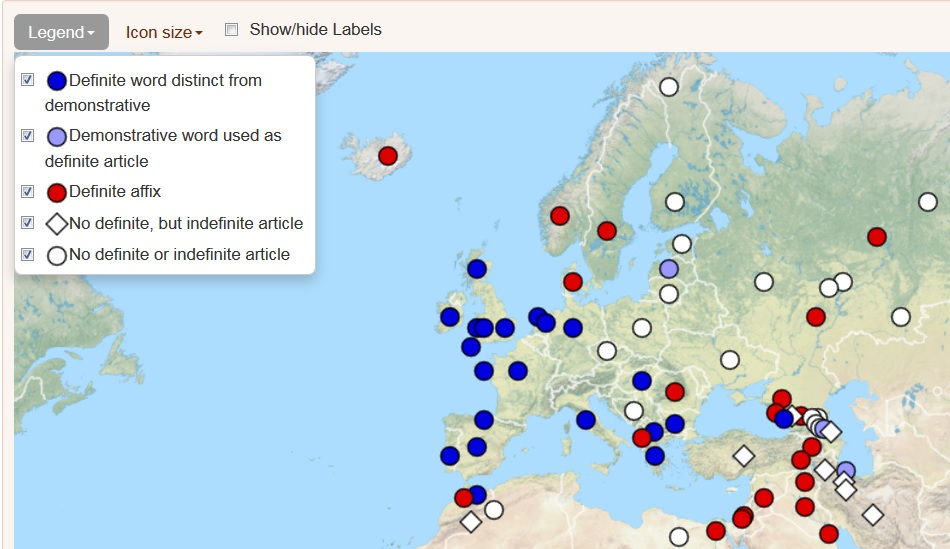
\includegraphics[width=\textwidth]{images/wals.jpg}
\caption {Definitartikel in den Sprachen Europas \parencite{Dryer2013}}
\label{wals}
\end{center}
\end{figure} 

Dargestellt ist die Verteilung von Demonstrativ-, Definit- \is{Demonstrativartikel}  \is{Definitartikel} und Indefinitartikeln \is{Indefinitartikel} in den Sprachen Europas: Hellblau markiert sind Sprachen, in denen das \isi{Demonstrativum} Aufgaben eines Definitartikels übernimmt. Dies ist bspw. im westlettischen Dialekt Tahmisch der Fall \parencite[573--574]{Schroeder2006}.
Eine funktionale \isi{Polysemie} wie diese hat in vielen Sprachen dazu geführt, dass sich das \isi{Demonstrativum} formal abspaltet und zum  \isi{Definitartikel} wandelt, so etwa in den (auf der Karte mit einem dunkelblauen Punkt gekennzeichneten) romanischen und westgermanischen Sprachen. Mit zunehmendem Gebrauch kann der \isi{Definitartikel} an lautlicher Substanz 
verlieren \is{Affigierung} und sich zur Flexionsendung entwickeln, wie bspw. in den  nordgermanischen Sprachen, vgl. schwed. \object{bok-en} \extrans{das Buch}, die in der Karte mit einem roten Punkt markiert sind.  Die formale Reduktion wird mit einer späten Entwicklungsstufe des Definitartikels gleichgesetzt. Das Verhältnis von Sprachen mit und Sprachen ohne \isi{Definitartikel} hält sich den Daten des WALS zufolge \parencite[Kapitel 37]{Dryer2013} in etwa die Waage (216 zu 198). Ob sich ein \isi{Definitartikel} herausbildet, ist von vielen sprachinternen und -externen Faktoren abhängig. Die slawischen Sprachen verfügen z.B. über keinen Definitartikel, wohl aber über Mittel, Referenten als definit zu kennzeichnen, bspw. mit Hilfe des Verbalaspekts \is{Verbalaspekt} oder durch Kasusoppositionen \is{Kasusopposition} \parencite{Hauenschild1993,Leiss2000}. Sprachen mit einer relativ freien Konstituentenabfolge (z.B. Finnisch oder Chinesisch) nutzen die \isi{Wortstellung}, um definite Referenten syntaktisch zu exponieren.\footnote{
Das ursprünglich artikellose Althochdeutsche verfügte über ähnliche Strategien, vgl. Abschnitt \ref{sec:def-ahd}.}

Nachfolgend geht es darum, die hier skizzierten Entwicklungsstufen vor dem Hintergrund grammatikalisierungstheoretischer \is{Grammatikalisierung} Ansätze zu diskutieren und damit den ersten Baustein für das theoretische Fundament der Arbeit zu schaffen. 
In Abschnitt \ref{sec:stufen} werden zunächst die wichtigsten Grammatikalisierungsskalen \is{Grammatikalisierungspfad} beleuchtet.  
Anschließend widmet sich Abschnitt \ref{sec:dem-quelle} dem besonderen Status des Demonstrativums \is{Demonstrativum} als Quelle für den Definitartikel. Abschnitt \ref{sec:parameter} nimmt die für den \isi{Definitartikel} wichtigsten Parameter der \isi{Grammatikalisierung} unter die Lupe. 


\subsection{Universelle Entwicklungsstufen}\label{sec:stufen}

In der Forschung wurden einige Modelle vorgeschlagen, die einerseits die Entwicklung vom Demonstrativ- \is{Demonstrativartikel} zum \isi{Definitartikel} erfassen und andererseits die formale und funktionale Weiterentwicklung des Artikels beschreiben. Die prominentesten stammen von \textcite{Greenberg1978} und daran anknüpfend \textcite{Lehmann2015} sowie \textcite{Schmuck2014}. Sie werden an dieser Stelle einführend vorgestellt und mit Blick auf ihre Anwendbarkeit für das Deutsche beleuchtet. Im Vordergrund steht dabei die frühe Phase der Artikelentwicklung. 
%
%\subparagraph*{Greenbergs Definitheitszyklus} 

Greenbergs \hervor{cycle of the definite article} \is{Grammatikalisierungspfad} \is{Definitheit} \parencite[61]{Greenberg1978} umfasst vier Stufen, welche in Abbildung~\ref{abb:greenberg} \parencite[entnommen aus][525]{deMulder2011} wiedergegeben sind.

\begin{figure}
%   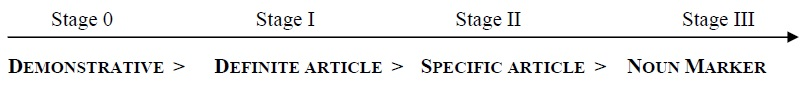
\includegraphics[width=9.5cm]{images/greenberg.jpg}
  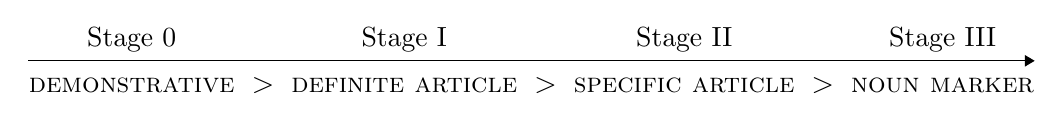
\begin{tikzpicture}[row 2/.style={font=\scshape}]
  \matrix (greenberg) [inner sep=0pt,matrix of nodes,row sep=.33cm,column sep=\tabcolsep]
    {
      Stage 0 & & Stage I & & Stage II && Stage III\\
      demonstrative & > & definite article & > & specific article & > & noun marker\\
    };
  \draw[-{Triangle[]}] (greenberg.west) -- (greenberg.east);
  \end{tikzpicture}
\caption {Der Definitheitszyklus \is{Grammatikalisierungspfad} \is{Definitheit} nach \textcite{Greenberg1978}\label{abb:greenberg}}
\end{figure}

Die Skala korreliert mit einem Abbau der \isi{Referentialität}: Aus einem \isi{anaphorisch} gebrauchten \isi{Demonstrativum} (Stage 0) wird ein Definitartikel, der dazu beiträgt, Referenten als identifizierbar zu kennzeichnen (Stage I). In der nächsten Stufe erfolgt die Ausweitung auf spezifische, \is{Spezifizität} aber nicht identifizierbare Referenten (Stage II), so dass der \isi{Definitartikel} in das Arbeitsfeld der Indefinita \is{Indefinitartikel} eindringt. Am Ende spielt die \isi{Referentialität} keine Rolle mehr: Der Artikel fungiert entweder als bloßer Genusmarker \is{Genus} oder -- und dies ist der Fall, wenn das ursprüngliche \isi{Demonstrativum} das Nomen nicht nach \isi{Genus} klassifiziert hat -- als Marker der \isi{Nominalität} \parencite[Stage III;][69]{Greenberg1978}. In dieser Rolle hilft er bspw., deverbale Nomen zu kennzeichnen. Die Entwicklung wird in der Regel begleitet von einem graduellen phonetischen Schwund, was Affigierungsprozesse \is{Affigierung} nach sich ziehen kann und der Zyklus von Neuem beginnt. In vielen germanischen Sprachen erfährt das ursprüngliche \isi{Demonstrativum} bereits eine erneute formale Stärkung \parencite[302--303]{vanGelderen2007}. Häufig wird die deiktische Komponente mit Hilfe von Lokaladverbien \is{Adverb} neu aufgebaut \parencite[s.][]{Diessel1999}, so auch im Deutschen (etwa:  \object{der da, das hier}). 

Bemerkenswerterweise ist der Zyklus nicht das Resultat von Überlegungen, wie Demonstrativa \is{Demonstrativum} zu Definitartikeln als Marker von \isi{Definitheit} werden, sondern wie sich \isi{Definitartikel} zu Genusmarkern \is{Genus} entwickeln. Entsprechend steht der emergierende Artikel nach Greenberg vornehmlich im Dienste einer eindeutigen und regelmäßigen Genusmarkierung \is{Genus} am Nomen, welche von Affixen \is{Affix} am Nomen nicht mehr gewährleistet wird, so etwa in den Niger-Kongo-Sprachen \parencite[55, 62]{Greenberg1978}. Dass diese Erklärung zum Ursprung des Definitartikels nicht für alle Sprachen greift, haben zahlreiche Studien herausgestellt, welche den Übergang als komplexe Verschiebung innerhalb der Domäne der \isi{Definitheit} beschreiben \parencite[z.B.][]{Himmelmann1997,Lyons1999,Leiss2000,Demske2001}, vgl. hierzu ausführlich Abschnitt \ref{sec:gruende}.

Auch die grobe lineare Dreischrittigkeit \isi{Demonstrativum} -- \isi{Definitartikel} -- Spezifizierer \is{Spezifizität} ist nicht unproblematisch. Denn erstens verläuft in vielen Sprachen (so auch im Deutschen) die \isi{Spezifizität} orthogonal zur \isi{Definitheit}, s. die Beispiele in \REF{ex:spez-ortho} in Adaption an \textcite[245]{Studler2011}; vgl. auch \textcite{Lyons1999}. 

\begin{exe}
	\ex \label{ex:spez-ortho}   
	\begin{xlist}
		\ex \label{ex:kleid1} Er sucht einen Übersetzer.  (unspez./indef.) 
		\ex \label{ex:kleid2} Sie hat gestern ein Auto gekauft. (spez./indef.)
		\ex \label{ex:stud1} Der erste Anrufer bekommt einen Preis. (unspez./def.)
		\ex \label{ex:stud2} Der Nachtisch gestern war sehr gut. (spez./def.)
		\end{xlist}
\end{exe}

\noindent 
Zweitens müssen anscheinend nicht alle Stadien zwangsläufig durchlaufen werden: \textcite[107]{Himmelmann1997} und \textcite[139]{Diessel1999} merken z.B. an, dass nicht nur Definitartikel, sondern auch Demonstrativa \is{Demonstrativum} als spezifische \is{Spezifizität} Artikel fungieren können, vgl. das Beispiel in \REF{ex:guy} aus \textcite[533]{deMulder2011}. 
\begin{exe}
	\ex \label{ex:guy}   There was this guy in my class last quarter.
\end{exe}
\noindent 
Anders als im Deutschen schwingt hier keine pejorative Lesart mit, sondern die Phrase \object{this guy} dient zur Einführung eines neuen und für den späteren Diskurs wichtigen Referenten. In diesem Fall wurde Stage I also übersprungen. 

Zudem müsste die letzte Entwicklungsstufe (Stage III) weiter ausdifferenziert werden. So kann der deutsche \isi{Definitartikel} gegenwärtig zwar als nominaler Marker \is{Nominalität} betrachtet werden -- etwa wenn er Eigennamen \is{Eigenname} begleitet (\object{die Pia}) oder Substantivierungen \is{Substantivierung} (\object{das Laufen}) kenntlich macht \parencite[71]{Szczepaniak2011a}. Andererseits zeigt er auch Tendenzen, sich zu einem \object{classifier} zu entwickeln, indem er u.a. ontologische (\object{die Bismarck} = Schiffsname) oder sozio-pragmatische Klassifikationen (z.B. denunziatorisch: \object{die Merkel}) über unterschiedliche Genera \is{Genus} abbildet \parencite{Nubling2014}. Greenberg selbst merkt an, dass Phasen parallel verlaufen können und es sich um einen graduellen Prozess mit möglichen Ausnahmen handelt \parencite[61]{Greenberg1978}. Nur über empirische Forschungen, idealerweise mit Blick auf diachrone Etappen von einzelnen Sprachen, kann dieser Prozess hinreichend beschrieben werden. 

Im Gegensatz zu Greenbergs Modell, das die Frühphase der Artikelentwicklung kaum thematisiert, setzt die darauf aufbauende Skala \is{Grammatikalisierungspfad} von \textcite{Lehmann2015} eine Stufe zwischen  Demonstrativ- \is{Demonstrativartikel} und \isi{Definitartikel} an und eröffnet damit Raum für Diskussionen, wie der kategoriale Wandel ablaufen könnte. Lehmann selbst kommentiert diesen Aspekt allerdings nur relativ kurz, indem er anmerkt:\hervor{[T]he demonstrative component is gradually reduced to mere definiteness, and the result is a definite article} \parencite[41]{Lehmann2015}. Sein Modell ist in Abbildung~\ref{abb:lehmann} wiedergegeben. 

\begin{figure}
\smartdiagramset{border color=black,
set color list={white,white,white,white,white},
uniform arrow color=true,
arrow color=black,
back arrow disabled=true}
\resizebox{\textwidth}{!}{\smartdiagram[flow diagram:horizontal]{demonstrative determiner, weakly demonstrative definite determiner, definite article, affixal article, noun marker}}
\caption {Der \isi{Grammatikalisierungspfad} von \textcite[59]{Lehmann2015}\label{abb:lehmann}}
\end{figure}

Aus Lehmanns Sicht bildet der anaphorische \is{anaphorisch} \isi{Demonstrativartikel} den Ausgangspunkt für die Entwicklung des Definitartikels \parencite[ebenso:][]{Greenberg1978,Lyons1999}. Seit der Monographie von \textcite{Himmelmann1997} wird auch der anamnestische Gebrauch \is{anamnestisch} als \hervor{Sprungbrett} für die \isi{Grammatikalisierung} \parencite[74]{Szczepaniak2011a} betrachtet \parencite[s. hierzu auch den Überblick in][527]{deMulder2011}. Für viele Sprachen fehlen jedoch Studien, die diese Entwicklungsstufe empirisch dokumentieren und mögliche  Brückenkontexte \is{Brückenkontext} \parencite[84]{Heine2002a} offenlegen, so auch für das Deutsche. Eine ausführliche  Auseinandersetzung mit diesem Aspekt erfolgt in Abschnitt \ref{sec:bruecke} der vorliegenden Arbeit.

Kritisch an Lehmanns \isi{Grammatikalisierungspfad} ist die Vermischung von formalen und funktionalen Aspekten des Wandels. Seine Skala suggeriert nämlich, dass die Stufe des affigierten \is{Affix} Artikels eine diskrete, eigenständige Phase ist. Der Verlust an phonetischer Substanz ist jedoch ein Beiprodukt, das -- abhängig von den typologischen Eigenheiten einer Sprache \parencite[vgl.][33]{Himmelmann2004} -- mit jeder Entwicklungsstufe einhergehen kann. Beispielsweise treten schon im  Althochdeutschen Präpositionen-Artikel-Klisen \is{Klitikon} auf, etwa \object{zi themo} > \object{zemo} \extrans{zu dem} \parencite{Schlachter2015}, also zu einer Zeit, in der der \isi{Definitartikel} erst am Anfang der \isi{Grammatikalisierung} steht. Bis heute liegt hier eine \hervor{Grammatikalisierungsbaustelle}   \parencite{Nubling1992,Nubling2005} vor, da die Verschmelzung u.a. durch phonologische und semantische Faktoren blockiert wird \parencite[s. auch][91]{Szczepaniak2011a}.
Entscheidend für den kategorialen Übergang von Demonstrativ- \is{Demonstrativartikel} zu \isi{Definitartikel} ist also die funktionale Seite des Wandels. \textcite{Schmuck2014} schlagen mit der Skala in Abbildung~\ref{abb:schmuckszczep} \parencite[aufbauend auf][]{Lyons1999,Szczepaniak2011a} einen \isi{Grammatikalisierungspfad} vor, der die funktionale Seite des Wandels in Bezug auf das ahd. \object{dër} \extrans{dieser} beschreibt. 

\begin{sidewaysfigure}
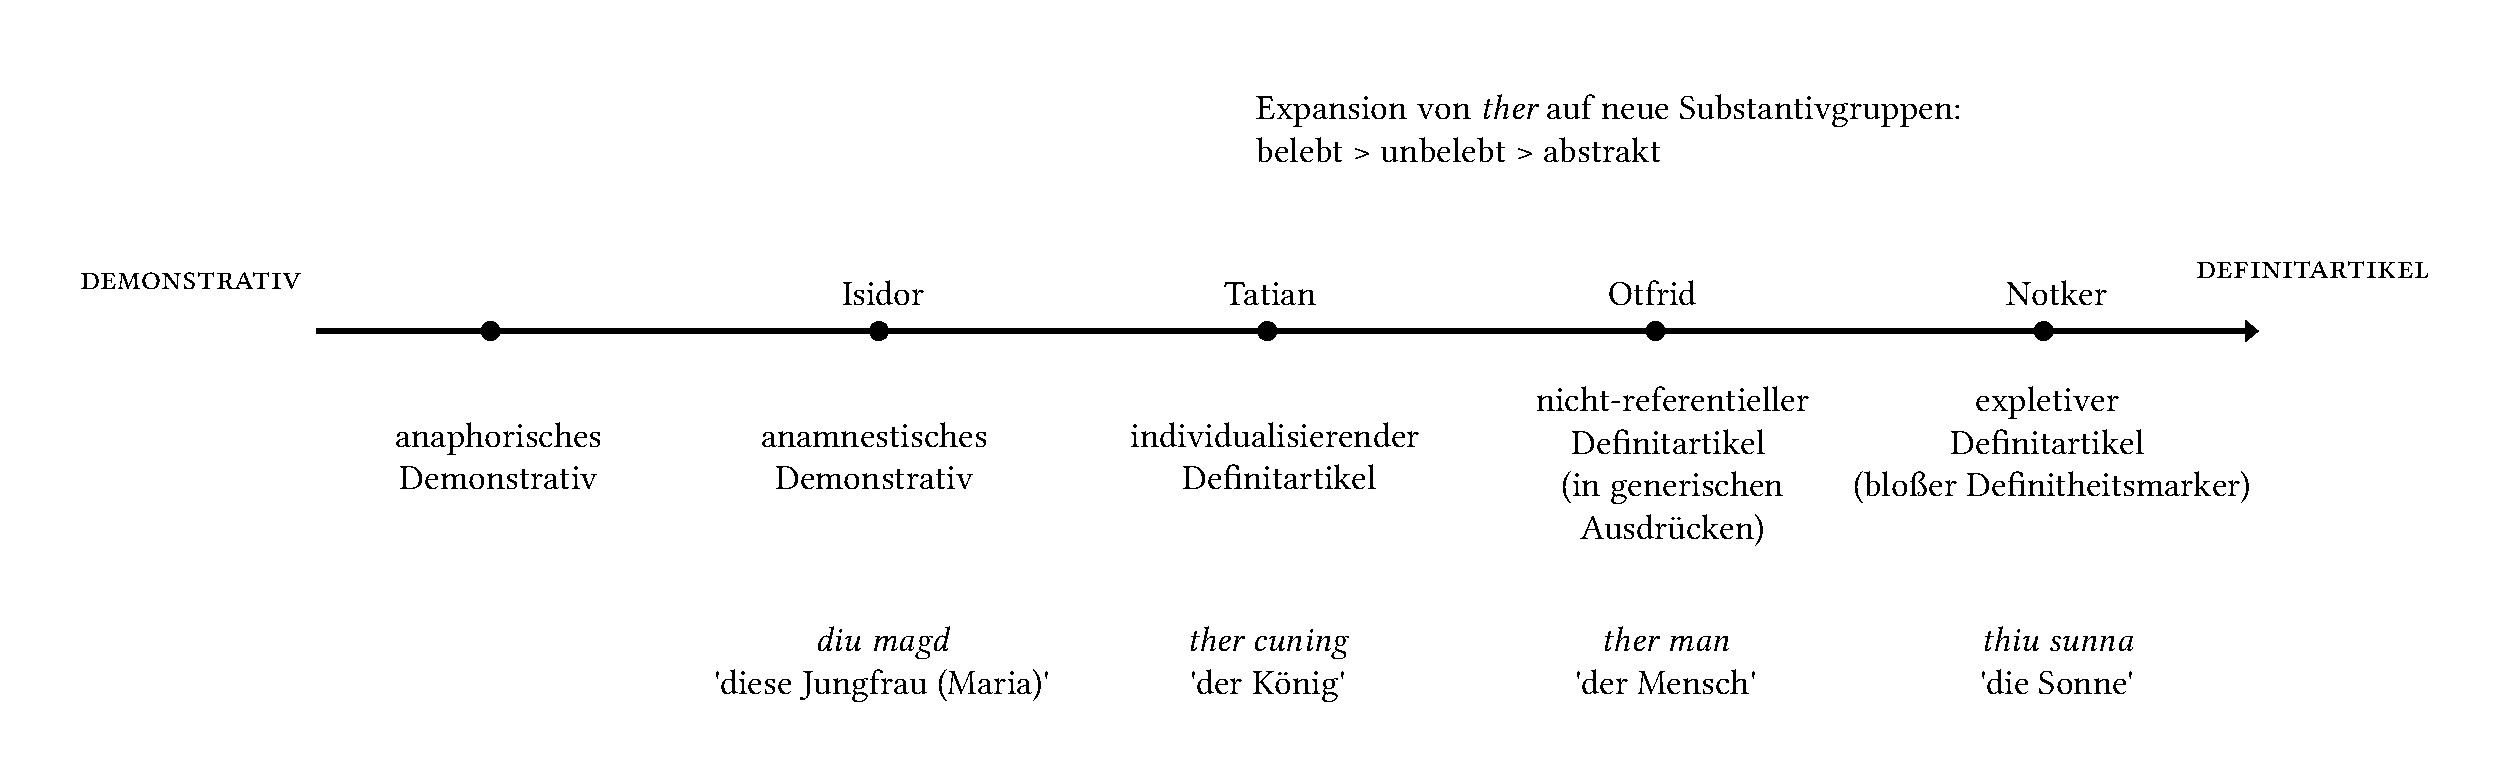
\includegraphics[width=\textwidth]{images/schmuckszczep.pdf}
\caption {Die \isi{Grammatikalisierung} des Definitartikels im Ahd. \parencite[102]{Schmuck2014}\label{abb:schmuckszczep}}
\end{sidewaysfigure}
 
Die Skala bildet die folgenden Entwicklungsstufen ab \parencite[vgl. auch][69--78]{Szczepaniak2011a}: Im frühen Althochdeutschen (repräsentiert durch Isidor, der um 780 entstanden ist), wird das \isi{Demonstrativum} vornehmlich gebraucht, um einen Referenten mittels Diskursinformationen (anaphorischer Gebrauch) \is{anaphorisch} oder mit Bezug auf gemeinsames Vorwissen (anamnestischer Gebrauch) \is{anamnestisch} \is{Definitheitskontext} von anderen potentiellen Referenten abzugrenzen. Das Herstellen solcher kontextabhängigen Bezüge ist charakteristisch für Demonstrativa \is{Demonstrativum} \parencite[85]{Himmelmann1997}. Im Laufe der Zeit verliert das Artikelwort  seine demonstrative Komponente und es wird möglich, auch ohne Kontext die eindeutige Referenz zu markieren (individualisierender Gebrauch). Damit ist der Weg für Gebrauchskontexte geebnet, die ausschließlich Definitartikeln vorbehalten sind, darunter nicht-referentielle (generische) Gebrauchskontexte \is{generisch} sowie die Kombination mit Unika \is{Unikum} (expletiver Artikel), \is{expletiver Artikel} die \textcite{Oubouzar1989,Oubouzar1992} schon bei Otfrid (um 870) und regelmäßiger bei Notker (um 1025) beobachtet. Die nächste Entwicklungsstufe ist die Ausweitung auf den onymischen Wortschatz, \is{Eigenname} die allerdings erst im Frühneuhochdeutschen (Frnhd.) einsetzt \parencite[s. ausführlich][]{Schmuck2014}. 

Ein zentrales Ziel der vorliegenden Arbeit ist es, die hier skizzierten Definitheitskontexte, \is{Definitheitskontext} welche in Kapitel \ref{chap:demdef} noch ausführlich beschrieben werden, mithilfe einer computergestützten Korpusanalyse in Bezug auf das ahd. \object{dër} zu untersuchen. Das Modell von \textcite{Schmuck2014} fungiert als theoretischer Ausgangspunkt und wird in Kapitel \ref{bicpic} auf Basis der gewonnenen Ergebnisse modifiziert. Wie man in Abbildung~\ref{abb:schmuckszczep} sieht, gehen \textcite{Schmuck2014} davon aus, dass die \isi{Expansion} des Definitartikels belebtheitsgesteuert \is{Belebtheit} (belebt > unbelebt > abstrakt) verläuft. Diese Hypothese wird auch in der vorliegenden Arbeit aufgenommen. Kapitel \ref{chapter:belebtheit} erläutert die Verbindung von Belebtheit \is{Belebtheit} und Artikelsetzung ausführlich. 

 
\subsection{Primäre oder sekundäre Grammatikalisierung?} \label{sec:dem-quelle}

Am Anfang von Grammatikalisierungsprozessen \is{Grammatikalisierung} stehen typischerweise lexikalische Elemente \parencite[s. ausführlich][]{Heine1991,Hopper1991,Traugott1991,Bybee1994,Lehmann2015}:  \blockcquote[4]{Bybee1994}{Reduced to its essentials, grammaticalization theory begins with the observation that grammatical morphemes develop gradually out of lexical morphemes or combinations of lexical morphemes with lexical or grammatical morphemes}. 
Ein klassisches Grammatikalisierungsbeispiel ist die Entwicklung von Vollverben zu Hilfsverben: So entwickelt sich das \object{going-to}-Futur z.B aus dem Vollverb \object{gehen} \parencite[s.][70--71]{Heine1991}. Der funktionale Shift wird meist von formalen Reduktionsprozessen \is{Klitikon} begleitet (\object{going to} > \object{gonna}) und führt durch die graduelle semantische Ausbleichung \parencite{Heine2003} zur steten Kontextausweitung \parencite{Himmelmann2004}.  

Mit Blick auf den Ursprung handelt es sich also beim Wandel vom Demon"-stra"-tiv- zum \is{Demonstrativartikel} \isi{Definitartikel} um einen speziellen Grammatikalisierungsprozess. Vereinfacht gesprochen entwickelt sich aus einem bereits vorhandenen grammatischen Element (dem Demonstrativartikel) eine neue grammatische Form. Dieser Prozess wird daher auch \object{sekundäre} \isi{Grammatikalisierung} \parencite{Givon1991, Detges2002, Szczepaniak2011a} genannt -- im Kontrast zu \object{primären} Grammatikalisierungen, an deren Beginn lexikalische Elemente stehen \parencite[81]{Traugott2002}.
Es ist allerdings fraglich, ob die sekundäre \isi{Grammatikalisierung} als eigene Entwicklungsstufe betrachtet werden sollte, die zeitlich auf eine frühere \isi{Grammatikalisierung} folgt. Für Givón, der den Terminus Anfang der 1990er in den Forschungsdiskurs einführt, ist eine solche Chronologie definitorisch: \blockcquote[][193]{Givon1991}{What is suggested in this article is that exis"-ting, earlier-grammaticalized morpho-syntax can give rise, via secondary grammaticalization, to other morpho-syntactic patterns}.

In Bezug auf die \isi{Grammatikalisierung} des Definitartikels \is{Definitartikel} lassen sich einige Argumente gegen die Annahme anführen, dass es eine lexikalische Quelle für das \isi{Demonstrativum} gibt und damit eine primäre \isi{Grammatikalisierung} der Entwicklung des Definitartikels vorausgeht: Laut \textcite[150]{Diessel1999} wurde bislang für keine Sprache der empirische Nachweis erbracht, dass Demonstrativa \is{Demonstrativum} von lexikalischen Elementen abstammen (die o.g. Strategien zur Stärkung der deiktischen Komponenten ausgenommen). Interessanterweise verfügen aber alle Sprachen über Demonstrativa \is{Demonstrativum} \parencite[1]{Diessel1999}. Neben Inhaltswörtern wie \object{Mama} oder \object{Ball} zählen demonstrative Ausdrücke zum frühen Wortschatz von Kindern; oft gehören sie zu den ersten zehn Wörtern, die erlernt werden \parencite[476]{Diessel2006}. Beides spricht dafür, Demonstrativa \is{Demonstrativum} zum linguistischen Grundinventar zu zählen. Auch funktional nehmen Demonstrativa \is{Demonstrativum} eine Sonderrolle ein: Während typische grammatische Elemente (z.B. Präpositionen) innersprachliche Relationen zwischen Lexemen anzeigen (z.B. \object{auf/unter/über dem Tisch}), liegt die Funktion von Demonstrativa \is{Demonstrativum} darin, die Aufmerksamkeit von Adressaten auf bestimmte Objekte in der außersprachlichen Umgebung zu lenken \parencites{Diessel2006}. 
%[152]{Diessel1999}
Auch innersprachlich sind Demonstrativa \is{Demonstrativum} zentrale diskursstrukturierende Mittel: Mit ihnen werden prominente Referenten anaphorisch \is{anaphorisch} wiederaufgenommen oder Topikwechsel eingeleitet. Wie in Abschnitt \ref{sec:kata} noch gezeigt wird, ist es gerade diese kommunikative Zeigefunktion, welche die \isi{Grammatikalisierung} überhaupt erst ankurbelt: Sprecherinnen und Sprecher nutzen sie aus, um wichtige, d.h. in erster Linie belebte und agentive Referenten \is{Belebtheit} zu exponieren. Der inflationäre Gebrauch führt dazu, dass sich die Zeigefunktion langsam abnutzt und auch Referenten, die auf der Belebtheitsskala \is{Belebtheitshierarchie} hierarchisch niedriger angesiedelt sind, regelmäßig mit dem emergierenden Artikel \is{Definitartikel} determiniert werden (vgl. hierzu ausführlich Kapitel \ref{chapter:belebtheit}).


\textcite{Breban2014} argumentiert plausibel dafür, dass eine Zweiteilung in primäre und sekundäre \isi{Grammatikalisierung} schließlich keinen definitorischen Mehrwert liefert.
Stattdessen plädiert sie für eine breitere Auslegung von Grammatikalisierung, die auch grammatische Elemente als mögliche Quelle für den Wandel in Betracht zieht und damit die Artikelentwicklung als \isi{Grammatikalisierung} einschließt  \parencite[zur weiterführenden Diskussion s.][]{Breban2012}: \blockcquote[498]{Breban2014}{[G]rammaticalization processes can have lexical, grammatical, or grammaticalized items/constructions as input. Whatever the nature of the input, the subprocesses of changes involved appear to be the same. [...] [G]ramma\-ticalization processes consist of a complex of changes that affect different domains of change, and happen at different stages in the grammaticalization process.}

\noindent 
Um die Charakteristika des Wandels und die im Zitat genannten \object{domains of change} zu erfassen, wurden in der Grammatikalisierungsforschung unterschiedliche Parameter \is{Grammatikalisierungsparameter} vorgeschlagen, die nachfolgend mit Blick auf die Entwicklung des Definitartikels diskutiert werden.   


\subsection{Parameter der Grammatikalisierung}\label{sec:parameter}

Nach \textcite[96--112]{Traugott2013} lassen sich zwei Hauptzweige in der Grammatikalisierungsforschung unterscheiden. Zum einen existiert ein großes und traditionsreiches Forschungsfeld \parencite[hierzu zählen u.a. die Arbeiten von][]{Givon1979,Haspelmath2004,Lehmann2015,}, in dem \isi{Grammatikalisierung} vor allem als gradueller Autonomieverlust des betroffenen sprachlichen Zeichens betrachtet wird, begleitet von formalen Reduktionsprozessen. Der andere Forschungszweig begreift \isi{Grammatikalisierung} als Prozess der Kontextexpansion \is{Expansion} \parencite{Himmelmann1997,Himmelmann2004}. 

Die Lehmannschen Grammatikalisierungsparameter \is{Grammatikalisierungsparameter} sind für die erste genannte  Forschungsrichtung exemplarisch, s. Tabelle~\ref{tab:lehmann-parameter-prozess}, entnommen aus \textcite{Lehmann1995}. Mit ihnen kann man sprachliche Zeichen hinsichtlich ihres Grammatikalisierungsgrades auf syntagmatischer und paradigmatischer Ebene vergleichen. 

%
\begin{table}
\centering
\small
\begin{tabular}{
	l
	>{\raggedright}p{2,75cm}
	c
	>{\raggedright\arraybackslash}p{2,75cm}
}
\lsptoprule
& \multicolumn{3}{c}{{Grammatikalisierungsgrad}}\\
                   & \multicolumn{1}{c}{{niedrig}}& & \multicolumn{1}{c}{{hoch}}\\
\cmidrule(lr){2-4}
{Parameter} & & {Prozess}   &                   \\ \midrule
{Paradigmatizität}            & Zeichen gehört zu losem Wortfeld                         & Paradigmatisierung & Zeichen gehört zu hochintegriertem Paradigma                     \\
{Wählbarkeit}                 & Zeichen ist nach kommunikativen Absichten frei wählbar   & Obligatorisierung  & Wahl des Zeichens ist beschränkt bzw. obligatorisch              \\
{Integrität}                  & Bündel semantischer Merkmale; evtl. mehrsilbig           & Erosion            & grammatische Merkmale; oligo- oder monosegmental                 \\
{Fügungsenge}                 & Zeichen ist unabhängig juxtaponiert                      & Koaleszenz         & Zeichen ist \isi{Affix} oder bloß phonologische Eigenschaft des Trägers \\
{Stellungsfreiheit}           & Zeichen ist frei umstellbar                              & Fixierung          & Zeichen besetzt feste Position                                   \\
{Skopus}                      & Zeichen bezieht sich auf Syntagma beliebiger Komplexität & Kondensierung      & Zeichen modifiziert Stamm                                        \\ \lspbottomrule
\end{tabular}
\caption{Parameter und Prozesse der \isi{Grammatikalisierung} \parencite[1255]{Lehmann1995}}
\label{tab:lehmann-parameter-prozess}
\end{table}

 
Der \isi{Definitartikel} zeigt im Gegenwartsdeutschen gemäß dieser Parameter \is{Grammatikalisierungsparameter} einen im Vergleich zu seinem demonstrativen Vorläufer erhöhten Grammatikalisierungsgrad. \is{Grammatikalisierung}

\begin{description}
\item[Paradigmatizität:] Der \isi{Definitartikel} bildet in Opposition zum \isi{Indefinitartikel} eine geschlossene grammatische Klasse, die im Ahd. nicht gegeben ist. Das Zahlwort \object{eins} entwickelt sich erst im Laufe des Mittelhochdeutschen (Mhd.) zum \isi{Indefinitartikel} \parencite{Szczepaniak2016}. 
\item[Wählbarkeit:] Im Ahd. konnte der \isi{Demonstrativartikel} relativ frei nach dem kommunikativen Ermessen der Sprecherinnen und Sprecher gesetzt werden \parencite{Oubouzar1992}. Im Gegenwartsdeutschen ist die Determinierung des Nomens mit Artikelwort die Regel. 
\item[Integrität:] Durch seine ursprünglich deiktischen und demonstrativen Komponenten vereint der \isi{Demonstrativartikel} mehr semantische Merkmale als der heutige Definitartikel, dessen Bedeutung abstrakter ist und -- vereinfacht gesagt-- auf \isi{Definitheit} reduziert wurde \parencite[41]{Lehmann2015}.
\item[Fügungsenge:] Unauflösbare Präpositionen-Artikel-Enklisen (z.B. \object{im, am}) \is{Klitikon} im Gegenwartsdeutschen zeigen, dass der Artikel an Autonomie eingebüßt hat und damit das Potential besitzt, sich zu einem Flexionsaffix \is{Affix} weiterzuentwickeln \parencite[s. hierzu][]{Nubling1992,Nubling2005}.  
\item[Stellungsfreiheit:] Der \isi{Demonstrativartikel} kommt im Ahd. sowohl prä- als auch postnominal vor \parencite[27--28]{Schrodt2004} und ist damit syntaktisch unabhängiger als der gegenwärtige Definitartikel, dessen Stellung vor dem nominalen Kern fixiert ist. \is{Wortstellung}
\item[Skopus:] Als Substantivmarker (z.B. \object{das Lernen}) beschränkt sich der \isi{Skopus} des Definitartikels nur noch auf Wortebene \parencite[71]{Szczepaniak2011a}. In klitisierter Form \is{Klitikon} kann der Artikel nicht über restriktive Nebensätze operieren: \object{Sie geht ?zum/zu dem Zahnarzt, der ihr empfohlen wurde.} \parencite[112]{Nubling2005}.
\end{description}

\noindent
Neben der Stellungsfreiheit \is{Wortstellung} und der Integrität ist für die Untersuchung des ahd. Demonstrativums \is{Demonstrativum} die Wählbarkeit der wohl wichtigste Aspekt. Denn wenn das Artikelwort nicht mehr variabel, sondern obligatorisch gesetzt wird, bildet es zusammen mit dem Bezugsnomen eine feste Einheit zum Ausdruck definiter Referenz \is{Definitheit} [\object{dër}\,+\,N] (s. Abschnitt \ref{sec:konstruktionalisierung}). 

Lehmanns strukturalistisch angelegte Parameter \is{Grammatikalisierungsparameter} prägen ein Grammatikalisierungsbild, das den Autonomieverlust eines einzelnen sprachlichen Zeichens in den Vordergrund stellt. Pragmatische Aspekte des Wandels und insbesondere metaphorische \is{Metapher} und metonymische \is{Metonymie} Kommunikationsstrategien, die Grammatikalisierungen \is{Grammatikalisierung} vorantreiben, werden dabei wenig beachtet. Dabei zeigen z.B. \textcite[84--93]{Hopper2006}, dass metonymische \is{Metonymie} Prozesse für kontext-indizierte Implikaturen sorgen, die bspw. die Entwicklung des \object{going-to}-Futurs bewirken. Die analogische Ausbreitung \is{Analogie} verläuft in diesem Fall entlang der metaphorischen \is{Metapher} Abstraktion \textsc{Raum > Zeit}\footnote{Die Kapitälchen kennzeichnen \blockcquote[85]{Hopper2006}{abstract, cross linguistic meanings, as opposed to language specific lexical items}.} \parencite[s. auch][45--46]{Heine1991}. Abschnitt \ref{sec:mechanismen} liefert eine ausführliche Diskussion der Rolle von \isi{Analogie} und \isi{Reanalyse} in Bezug auf den Definitartikel. 

Ein weiteres wichtiges Prinzip der Grammatikalisierung, das \citeauthor{Lehmann1995}s Modell nicht direkt abbildet, ist die Tatsache, dass ein Sprachzeichen durch die graduelle semantische Ausbleichung  (in \citeauthor{Lehmann1995}s  Terminologie die \object{Erosion}) im Laufe der Zeit ein immer größeres Spektrum an Gebrauchskontexten abdecken kann und frühere Restriktionen ablegt. Dies lässt sich ebenfalls am \object{going-to}-Futur illustrieren: Während ursprünglich  nur bewegungsfähige Subjekte \is{Subjekt} möglich waren (etwa: \object{I am going to the store}), können heute auch unbelebte Referenten \is{Belebtheit} in der Subjekts"-position vorkommen \is{Subjekt} \parencite[etwa: \object{The tree is going to lose its leaves}; Beispiele nach][5--6]{Bybee1994}. 

\textcite{Himmelmann1997,Himmelmann2004} entwickelt vor diesem Hintergrund ein Sprachwandelkonzept, in dem \isi{Grammatikalisierung} als "`process of context-expansion"'\linebreak \parencite[32]{Himmelmann2004} \is{Expansion} verstanden wird. Damit gilt er als einer der Hauptvertreter des zweiten grammatikalisierungstheoretischen Zweigs, den \textcite[105--109]{Traugott2013} in ihrer Übersicht anführen. Nach \citeauthor{Himmelmann2004} gibt es drei Arten der Kontextexpansion, die \is{Expansion} \object{host-class expansion}, die \object{syntactic context expansion} und die \object{semantic-pragmatic context expansion}, die er am Beispiel des Definitartikels erläutert \parencite[s.][32--33]{Himmelmann2004}: 

\begin{description}
\item[Host-class expansion:] Lockerung der Kollokationsbeschränkungen und damit\linebreak steigende Kombinierbarkeit des grammatikalisierenden Elementes auf syntagmatischer Ebene: Der \isi{Definitartikel} erscheint mit immer mehr Substantivklassen. Dadurch wird u.a. die schrittweise Kombination mit Unika \is{Unikum} oder Eigennamen \is{Eigenname} möglich, welche das ursprüngliche \isi{Demonstrativum} nicht leisten kann. 
\item[Syntactic context expansion:] Anstieg \is{Expansion} der größeren syntaktischen Kontexte, in denen der grammatikalisierende Ausdruck erscheint: Der emergierende \isi{Definitartikel} ist \textcite[32]{Himmelmann2004} zufolge zunächst auf die Subjekts- und Objektsposition \is{Subjekt} \is{Objekt} beschränkt und kann dann in weniger zentrale Argumentpositionen (z.B. Adverbiale) \is{Adverbial} expandieren \is{Expansion} \parencite[s. hierzu auch ausführlich][]{Himmelmann1998}. 
\item[Semantic-pragmatic context expansion:] Anstieg \is{Expansion} der Gebrauchskontexte, in de-\linebreak nen der Ausdruck gewählt wird: Beim emergierenden \isi{Definitartikel} kommen zu den ursprünglichen pragmatisch-definiten (situationsabhängigen) Gebrauchskontexten semantisch-definite (situationsunabhängige) Ge-\linebreak brauchskontexte hinzu. \is{Pragmatische Definita} \is{Semantische Definita} \is{Definitheitskontext}

 
\end{description}

\noindent
Die Expansionstypen \is{Expansion} bedingen sich gegenseitig: Der Abbau von semantischen Merkmalen (und der gleichzeitige Aufbau neuer grammatischer Funktionen) führt dazu, dass ein Zeichen in immer neuen syntaktischen Kontexten verwendet werden kann. Umgekehrt hat jeder Gebrauch in neuen Kontexten zur Folge, dass sich die neue Funktion etabliert. Die graduelle Obligatorisierung der Form und die damit zusammenhängenden Reduktionsprozesse, die Lehmanns Modell hervorhebt, sind nach \textcite[33]{Himmelmann2004} lediglich Epiphänome des Wandels. Während die \herkur{host class expansion} \is{Expansion} von der \isi{Belebtheit}  beeinflusst wird (s. Kapitel \ref{sec:belebtwandel}), kommen bei der \herkur{syntactic context expansion} \is{Expansion} die semantische Rolle \is{Semantische Rolle} und damit zusammenhängend die \isi{Referentialität} als Faktoren ins Spiel (s. Abschnitt \ref{sec:partizipanten}).

Durch die bisherigen Ausführungen wurde bereits implizit deutlich, dass Sprachzeichen nur innerhalb bestimmter syntagmatischer Kontexte grammatikalisieren.\footnote{Eine Zusammenfassung der Grammatikalisierungsansätze, die explizit den Kontext hervorheben, bietet \textcite{Traugott2003,Traugott2008a}.} 
Diese Erkenntnis ist zwar nicht neu, sie führt aber zu einer wichtigen systemlinguistischen Präzisierung, welche Himmelmann in Bezug auf den \isi{Definitartikel} wie folgt darlegt: \blockcquote[31]{Himmelmann1997}{In Grammatikalisierungsprozessen \is{Grammatikalisierung} wird nicht nur ein Element, das Grammem, sondern ein Ausdrucksmuster (eine Konstruktion) grammatikalisiert. Folglich stellt die Formulierung \extrans{ein \isi{Demonstrativum} entwickelt sich zu einem Definitartikel} \is{Definitartikel} eine Verkürzung dar. Präziser formuliert besteht der Prozeß darin, daß das Ausdrucksmuster Nomen\,+\,Deiktikon sich zu einem Ausdrucksmuster Nomen\,+\,grammatikalisiertes D-Element\footnote{Mit \object{D-Elementen} sind adnominal gebrauchte Lokaldeiktika gemeint \parencite[6]{Himmelmann1997}.} 
 entwickelt.} 
Was Himmelmann vortheoretisch als \object{Konstruktion} \is{Konstruktion} bezeichnet, ist in kon\-struk\-tions\-grammatischen Ansätzen die zentrale Einheit von Sprachen \parencite[s. u.a.][]{Goldberg1995,Goldberg2006}. Daher erscheint es rückblickend fast als logische Konsequenz, dass die historische Sprachwissenschaft die Konstruktionsgrammatik für die\linebreak Sprach"-wandel"-for"-schung rekrutiert hat. Das Ergebnis ist die \object{diachrone Konstruktionsgrammatik} \parencite[vgl. u.a.][]{Barddal2015}, innerhalb derer die gängigen Grammatikalisierungstheorien maßgeblich weiterentwickelt wurden (s. hierzu u.a.\citealt{Traugott2003,Bergs2008,Diewald2008,Fried2013,Traugott2013}). Die vorliegende Untersuchung knüpft an diese Forschung an, indem die Entwicklung des Definitartikels als \object{\isi{Konstruktionalisierung}} betrachtet wird -- ein Prozess, der nachfolgend im Rahmen des hier verwendeten konstruktionsgrammatischen Ansatzes definiert wird.\footnote{Wenn im weiteren Verlauf der Arbeit von der Entwicklung des Definitartikels bzw. der Entwicklung von \object{dër} gesprochen wird, so sei an dieser Stelle darauf hingewiesen, dass damit immer die Entwicklung der Konstruktion \is{Konstruktion} [\object{dër}\,+\,N] von einer Demonstrativ- \is{Demonstrativartikel} \is{Konstruktion} zu einer Definitartikelkonstruktion gemeint ist.}  

\section{Die konstruktionsgrammatische Perspektive}\label{sec:kxg}
Um der Entwicklung des Definitartikels im Deutschen auf den Grund zu gehen, erhalten die grammatikalisierungstheoretischen Theorien nachfolgend einen konstruktionsgrammatischen \hervor{Überbau}. Insbesondere gebrauchsbasierte, kognitive  Arbeiten \parencite[u.a.][]{Langacker1987,Goldberg1995,Goldberg2006,Croft2002,Croft2004,Bybee2006,Bybee2010} stehen hierfür Pate.\footnote{Überblicksdarstellungen der verschiedenen Forschungsrichtungen, die zur Konstruktionsgrammatik zählen, sind zu finden in:   \textcite{Croft2004,Imo2007,Stefanowitsch2011,Hoffmann2013,Ziem2013}.} Zunächst werden in Abschnitt \ref{sec:kxg-grundlagen} die zentralen Prämissen der Konstruktionsgrammatik -- mit besonderem Augenmerk auf Synergieeffekte zur Grammatikalisierungstheorie -- erläutert. Anschließend geht es in Abschnitt \ref{sec:konstruktionalisierung} um den Unterschied zwischen Konstruktionswandel,  \isi{Konstruktionalisierung} und Grammatikalisierung. Es wird dafür argumentiert, dass es sich bei der Entwicklung des Definitartikels um einen Konstruktionalisierungsprozess \is{Konstruktionalisierung} handelt, der das Schema [Definitartikel\,+\,N] zum Ergebnis hat.  

\subsection{Prämissen der Konstruktionsgrammatik}\label{sec:kxg-grundlagen}

%\subsubsection{Konstruktionen als Basiseinheiten der Sprache} 

In der Konstruktionsgrammatik wird davon ausgegangen, dass sich das Inventar einer Sprache vollständig über Form-Bedeutungspaare, die Konstruktionen, erfassen lässt. Form und Bedeutung gehen eine (zumindest partiell) arbiträre und damit symbolische Beziehung ein \parencite[257]{Croft2004}. Zur Bedeutungsseite gehören dabei auch pragmatische und diskurs-funktionale Eigenschaften, s. Abbildung~\ref{abb:croft-construction}.  

\begin{figure}
% %   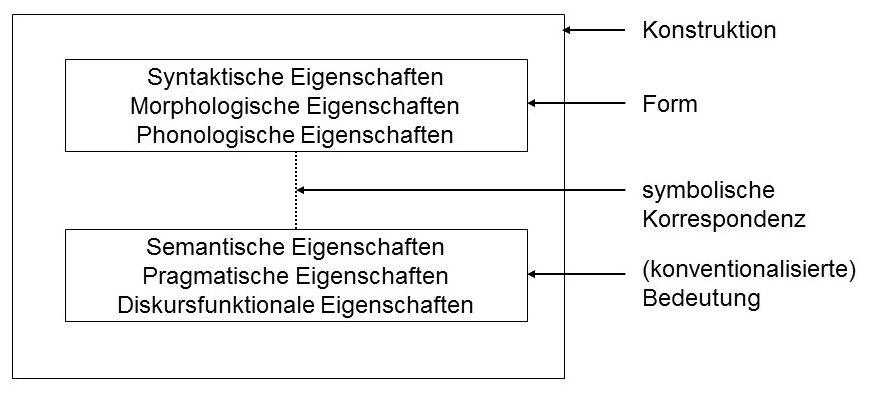
\includegraphics[width=9cm]{images/croft-construction-neu.jpg}
  \begin{tikzpicture}
  \node at (0,0) [draw,text width=7cm,align=center] (Eig1) 
    {Syntaktische Eigenschaften\\Morphologische Eigenschaften\\Phonologische Eigenschaften};
  \node [,draw, below=2\baselineskip of Eig1,text width=7cm,align=center] (Eig2) 
    {Semantische Eigenschaften\\Pragmatische Eigenschaften\\Diskursfunktionale Eigenschaften};
  \draw[dotted,thick] (Eig1) -- (Eig2) node[midway,name=midway] {};
  \node [draw,inner sep=.33cm,fit=(Eig1) (Eig2)] (konstr) {};
  \node [inner sep=0pt,right=.5cm of konstr.30] (Konstruktion) {Konstruktion};
  \path let \p1 = (Konstruktion.west), \p2  = (Eig1) in node [inner sep=0pt,anchor=west] at (\x1,\y2)
    (Form) {Form};
  \path let \p1 = (Konstruktion.west), \p2  = (midway) in node [text width=3.25cm,inner sep=0pt,anchor=west] at (\x1,\y2)
    (Korrespondenz) {symbolische\\Korrespondenz};
  \path let \p1 = (Konstruktion.west), \p2  = (Eig2) in node [text width=3.25cm,inner sep=0pt,anchor=west] at (\x1,\y2)
    (Bedeutung) {(konventionalisierte)\\Bedeutung};
  \draw[-{Triangle[]}] (Konstruktion.west) -- (konstr.30);
  \draw[-{Triangle[]}] (Form) -- (Eig1);
  \draw[-{Triangle[]}] (Korrespondenz) -- (midway);
  \draw[-{Triangle[]}] (Bedeutung) -- (Eig2);
  \end{tikzpicture}
\caption {Symbolische Struktur einer \isi{Konstruktion}  \parencite[18]{Croft2002}\label{abb:croft-construction}}
\end{figure} 

 Wenn ein Strukturmuster semantische oder formale Eigenschaften besitzt, die nicht"=kom"-po"-sitionell zustande kommen, diese also zusätzlich erlernt werden\linebreak müssen, liegt eine Konstruk"-tion vor \parencite[4]{Goldberg1995}. Ebenso, wenn ein sprachliches Muster besonders frequent gebraucht wird und sich dadurch eine mentale Repräsentation einschleift bzw. \object{entrenched} wird \parencite[93]{Goldberg2006}.\footnote{In Abschnitt \ref{sec:entrenchment} werden die für den \isi{Definitartikel} relevanten Prinzipien des \object{Entrenchment} ausführlich diskutiert.}
Konstruktionen können als primär grammatisch eingeordnet werden, wie es z.B. bei Hilfsverbkonstruktionen (etwa \object{going-to}-Futur) der Fall ist; sie führen dann relationale Funktionen aus und sind nicht-referentiell. Oder sie sind lexikalisch, wenn sie von referentieller und beschreibender Art sind \parencite[wie das Vollverb \object{gehen}, vgl.][58]{Traugott2015}. 

%\subsubsection{Lexikon-Grammatik-Kontinuum}

Grammatik und Lexikon einer Sprache sind keine autonomen Bereiche, sondern bilden ein Kontinuum. Dies ist die zweite wichtige Annahme, die sich aus dem oben beschriebenen  Konstruktionskonzept ergibt.\footnote{Argumente gegen die strikte Trennung von Grammatik und Lexikon liefern zahlreiche Studien, etwa \textcite{Goldberg2006}.} Ein Morphem kann beispielsweise abstrakt (z.B. ein Plu"-ral"=Morphem) oder spezifisch (z.B. \object{See}) sein. Das gleiche gilt für größere Einheiten. So repräsentieren z.B. spezifische Idiome (\object{das Handtuch werfen}) ebenso Instanzen von schematischen Strukturen wie die Transitivkonstruktion \is{Konstruktion}   (NP\textsubscript{Akk} \object{werfen}). Gemessen an ihrer Komplexität und ihrer Schematizität können Konstruktionen im Grammatik-Lexikon-Kontinuum verortet werden. Diese nicht-modulare Sicht auf Sprache hat den Vorteil, dass kategoriale Übergänge problemlos erfasst werden können, da sowohl grammatische als auch lexikalische Konstruktionen mit dem gleichen Analyseinstrumentarium behandelt werden. Eines der zentralen Anliegen in der Grammatikalisierungsforschung ist es, den Übergang von freien Syntagmen zu gebundenen grammatischen Zeichen zu modellieren. Aus diesem Grund ist die Konstruktionsgrammatik sehr gut mit der Grammatikalisierungstheorie kompatibel \parencite[zur weiterführenden Diskussion s. ][85]{Diewald2008}. 

%\subsubsection{Netzwerk von Konstruktionen}

Die Konstruktionen formen ein taxonomisch organisiertes Netzwerk, das sog. \object{Konstruktikon} \parencite[95]{Ziem2013}, in dem formal und/oder funktional ähnliche Konstruktionen miteinander assoziiert sind \parencites()()[]{Langacker1987}[262--265]{Croft2004}[]{Bybee2010}. Das Netzwerk ist dynamisch. Abhängig vom konkreten Sprachgebrauch können  Konstruktionen hinzukommen oder verschwinden. \textcite[17]{Traugott2013} unterscheiden dabei zwei Typen von Konstruktionen: die \object{item}-spezifischen Mikrokonstruktionen und die hierarchisch übergeordneten Schemata, welche ggf. Subschemata enthalten können \parencite[s. auch][]{Traugott2015}. Die im Sprachgebrauch empirisch beobachtbaren Token werden \object{constructs} genannt.\footnote{Zur Unterscheidung von \object{constructions} und \object{constructs} vgl. u.a. \textcite[][423]{Fried2013}.} Abbildung~\ref{abb:quant-schema} zeigt die Verlinkung dieser Ebenen am Beispiel des sog. \object{quantifier schema} \parencite[aus][17]{Traugott2013}. 

\begin{figure}
% % \tikzstyle{inner} = [shape=rectangle, rounded corners, draw, align=center, text width=10em]
% % \tikzstyle{level 1} = [sibling distance=10cm]
% % \tikzstyle{level 2} = [sibling distance=5cm]
% % \begin{tikzpicture}[level distance=2cm]
% %   \node[inner] {Schema\\ (z.B.~quantifier schema)}
% %     child { 
% %     	node[inner] {Subschema\\ (z.B.~large quantity)}
% %     	  child {
% %     	  	node[inner] {Mikro\-konstruktion~1}
% %     	  	  child {node {\object{many}}}
% %     	  }
% %     	  child {
% %     	  	node[inner] {Mikrokonstruktion~2}
% %     	  	  child {node {\object{a lot of}}}
% %     	  }
% %     } 
% %     child {
% %     	node[inner] {Subschema\\ (z.B. small quantity) }
% %     	  child {
% %     	  	node[inner] {Mikrokonstruktion~3}
% %     	  	  child {node {\object{few}}}
% %     	  }
% %     	  child {
% %     	  	node[inner] {Mikrokonstruktion~4}
% %     	  	  child {node {\object{a bit of}}}
% %     	  }
% %     };
% % \end{tikzpicture}
\resizebox{\textwidth}{!}{\begin{forest}
 [Schema\\ (z.B.~quantifier schema),align=center,draw,rounded corners
    [Subschema\\ (z.B.~large quantity),align=center,draw,rounded corners
      [Mikrokonstruktion 1,draw,rounded corners [\object{any}]]
      [Mikrokonstruktion 2,draw,rounded corners [\object{a lot of}]]
    ]
    [Subschema\\ (z.B. small quantity),align=center,draw,rounded corners
      [Mikrokonstruktion 3,draw,rounded corners [\object{few}]]
      [Mikrokonstruktion 4,draw,rounded corners [\object{a bit of}]]
    ]
 ]
\end{forest}}
\caption {Hierarchische Ordnung von Konstruktionen \is{Konstruktion}  (\object{quantifier schema})} 
\label{abb:quant-schema}
\end{figure}
 


An der Diachronie von [\object{a lot of}\,+\,N] lässt sich illustrieren, wie eine neue Mikrokonstruktion \is{Konstruktion} ihren Platz im Konstruktikon einnimmt: Ihre Ursprünge gehen auf das Altenglische \object{hlot} zurück, welches konkrete, unbelebte \is{Belebtheit} Objekte denotiert und als Partitivausdruck gebraucht wird, z.B. \object{hlot landes} \extrans{ein Stück Land} \parencite[230]{Traugott2008a}. Seit dem Mittelenglischen expandiert die Konstruktion \is{Konstruktion} auf  belebte \is{Belebtheit} Referenten (etwa \object{a lot of folks}). Als echter \object{quantifier} (wie z.B. in \object{a lot of power} \extrans{viel Macht}) kommt \object{a lot of} ab dem 19. Jh. zum Einsatz  und reiht sich in dieser nicht-partitiven Funktion neben seine Schwesterkonstruktion \object{many} ein \parencite[weiterführend s.][23--24]{Traugott2013}.


%\subsubsection{Gebrauchsbasierter Ansatz}
Durch Wiederholungen können spezifische Spracheinheiten konventionalisiert und neue Konstruktionsknoten im Netzwerk ausgebildet werden. Voraussetzung hierfür ist die menschliche Fähigkeit, Sprache mittels Erfahrung zu kategorisieren und über Abstraktionsprozesse spezifische Äußerungen mit schematischen Konstruktionen zu assoziieren. Konstruktionen werden vor diesem Hintergrund gebrauchsbasiert (\object{usage-based}) und auf Grundlage allgemeiner kognitiver Kategorien erworben \parencite[u.a.][]{Langacker1987,Goldberg2006,Bybee2006,Bybee2010,Bybee2013}.

In der Konstruktionsgrammatik wird Grammatik als dynamisches System aufgefasst, das kommunikationsbedingten Veränderungen ausgesetzt ist \parencite[35--36]{Imo2007}. Auch dieser Aspekt ist sehr gut mit der \isi{Grammatikalisierung} in Einklang zu bringen, man denke bspw. an den von  \textcite{Hopper1991} geprägten Begriff der \object{emergent grammar}. Individuelle Innovationen, die sich synchron als Sprachvariation niederschlagen \parencite{Croft2010}, haben das Potenzial, über den kognitiven Abgleich mit bestehenden Konstruktionen \object{sanktioniert} zu werden und Sprachwandel voranzutreiben \parencite[66]{Langacker1987}. 

\subsection{Konstruktionswandel und \isi{Konstruktionalisierung}}\label{sec:konstruktionalisierung}

Man kann zwei Arten von konstruktionsspezifischem Sprachwandel unterscheiden: den Konstruktionswandel und die \isi{Konstruktionalisierung} \parencite[vgl.][]{Hilpert2011,Hilpert2013,Fried2013,Traugott2013,Traugott2015,Trousdale2014}. 

Unter Konstruktionswandel fallen diejenigen Wandelprozesse, denen Mikrokonstruktionen, d.h. lexikalisch vordefinierte Konstruktionen unterworfen sind. Hierzu zählen Veränderungen auf der Form- oder Inhaltsseite, z.B. der graduelle Verlust der demonstrativen Komponente beim ursprünglichen \isi{Demonstrativum}  oder die Verschmelzungstendenzen von Präposition und \isi{Definitartikel} in der Gegenwartssprache (\object{in die} > \object{inne}, \object{zu dem} > \object{zum}). Konstruktionswandel liegt auch vor, wenn sich das Kollokationsverhalten und die Frequenz einer Mikrokonstruktion \is{Konstruktion} verändern. Im vorhergehenden Abschnitt wurde bereits angemerkt, dass die Entstehung neuer Kollokate (im Sinne von Himmelmanns \is{Expansion} \herkur{host-class expansion}, s. Abschnitt \ref{sec:parameter}) für die Herausbildung des Definitartikels konstitutiv ist. Was die Frequenz angeht, so kann man vor dem Hintergrund der zunehmenden Obligatorisierung ein Anstieg im Gebrauch von \object{dër} erwarten. 

Zudem subsummiert Konstruktionswandel im Vergleich zur \isi{Grammatikalisierung} eine breitere Palette an Wandelphänomenen: Erstens betrifft das Konzept nicht nur Konstruktionen, die sich in Richtung des grammatischen Pols einer Sprache wandeln. Auch Lexikalisierungsprozesse, die zur Bereicherung des lexikalischen Wortschatzes führen, z.B. in Form von Univerbierungen (\object{Tageslicht}) oder idiomatischen Wendungen (\object{ins Gras beißen}) zählen zum Konstruktionswandel \parencite[64]{Hilpert2011}, da sich auch hier form- oder funktionsseitige Veränderungen vollziehen. Während grammatische Konstruktionen im Laufe der Zeit an Schematizität und Produktivität gewinnen, büßen lexikalische Konstruktionen beides im Laufe ihrer Entstehung ein \parencite[vgl.][164]{Traugott2013}. Zweitens berücksichtigt Konstruktionswandel auch grammatische Wandelphänomene, die nicht den Charakteristika klassischer Grammatikalisierungen entsprechen, etwa Wortstellungswandel \parencite[vgl.][65]{Hilpert2011}. Weil Wortstellungsmuster \is{Wortstellung} ebenfalls als Konstruktionen begriffen werden (nämlich als abstrakte Schemata), können sie gleichermaßen das Resultat von Konstruktionswandel sein wie spezifische Mikrokonstruktionen. 

Wenn Konstruktionswandel dazu führt, dass sich in einer Sprache ein neues konventionalisiertes Form-Funktionspaar etabliert, sprechen \textcite{Traugott2013} von \isi{Konstruktionalisierung}. Sie definieren diesen Prozess folgendermaßen:  \blockcquote[22]{Traugott2013}{Constructionalization is the creation of form$_{new}$-meaning$_{new}$ (combinations of) signs. It forms new type nodes, which have new syntax or morphology and new coded meaning, in the linguistic network of a population of speakers. It is accompanied by changes in degree of schematicity,
productivity, and compositionality. The constructionalization of schemas
always results from a succession of micro-steps and is therefore gradual.
New micro-constructions may likewise be created gradually, but they may
also be instantaneous. Gradually created micro-constructions tend to be
procedural, and instantaneously tend to be
contentful.}

\noindent
Zu den \object{instantaneously created micro-constructions} zählen lexikalische Konstruktionen, denen kein Konstruktionswandel vorausgegangen ist. \textcite[3]{Traugott2013} führen hier u.a. Konversionen oder Entlehnungen an (etwa: \object{merkeln} oder \object{Sushi}). Solche Fälle sind für die vorliegende Untersuchung nicht weiter relevant. Denn bei der Entwicklung des Definitartikels handelt es sich um einen graduell ablaufenden Prozess, der aus einer Vielzahl von \object{micro-steps} zusammengesetzt ist und in der \isi{Konstruktionalisierung} des Schemas  [\object{dër}\,+\,N]  resultiert. Diese Mikroschritte werden in den nächsten Abschnitten erläutert und zwar erstens vor dem Hintergrund des in der Definition genannten Parameters der Schematizität (s. Abschnitt \ref{sec:schema}), welcher eng mit der Produktivität und Kompositionalität eines Sprachzeichens zusammenhängt sowie dem kognitiven Mechanismus des  \object{Entrenchment} (s.  Abschnitt \ref{sec:entrenchment}); zweitens mit Bezug auf die zentralen Mechanismen des Wandels: die \isi{Analogie} und \isi{Reanalyse} (s. Abschnitt \ref{sec:mechanismen}). 

Der entscheidende Vorzug der \isi{Konstruktionalisierung} liegt \textcite[60--62]{Traugott2015} folgend darin, dass sich die in Abschnitt \ref{sec:gram}  diskutierten Grammatikalisierungstheorien gut miteinander vereinen lassen: Während der eine Forschungszweig (mit \citealt{Lehmann1995} und \citealt{Haspelmath2004} als wichtige Vertreter) formale und/\-oder funktionale Reduktionsprozesse, wie sie typischerweise auf der Ebene der Morphosyntax und Morphonologie zu finden sind, fokussiert, betont der andere (vertreten u.a. durch \citealt{Himmelmann2004} und \citealt{Croft2006}), dass ein grammatisches Zeichen im Laufe seiner Entstehung an syntaktischer und semantisch-pragmatischer Reichweite gewinnt sowie neue Kollokationen zulässt; diese Perspektive inkludiert neben morphosyntaktischen auch diskursspezifische Wandelprozesse \parencite[vgl. den Begriff der \object{Pragmatikalisierung} für die Entwicklung von Diskursmarkern bei][]{Auer2005}. 

Mit der konstruktionsgrammatischen Sicht spielt es keine Rolle, welcher Bereich der Grammatik von Wandel erfasst wird, so dass der Konstruktionalisierungsbegriff \is{Konstruktionalisierung} weit genug ist, um alle genannten Ebenen einzubeziehen. Zudem kann man aus gebrauchsbasierter Perspektive dafür argumentieren, dass formale und funktionale Reduktionsprozesse in direktem Zusammenhang zur Kontextexpansion \is{Expansion} stehen und die beiden genannten Forschungsperspektiven im Prinzip zwei Seiten derselben Medaille ausmachen: So begünstigen semantische Ausbleichungsprozesse die schrittweise Ausbreitung in neue Gebrauchskontexte \parencite[61]{Traugott2015}. Und wenn eine Konstruktion \is{Konstruktion} häufig gebraucht wird, erhöht sich die Wahrscheinlichkeit, dass sie an phonetischer Substanz und auch an Kompositionalität einbüßt \parencite[20]{Bybee2010}.  Konstruktionsgrammatische Analysen tragen diesem vielschichtigen Wandel insofern Rechnung, als dass sie das Augenmerk sowohl auf die interne Struktur eines Sprachzeichens richten, d.h. auf die Charakteristika der einzelnen Konstituenten, als auch auf die externen Eigenschaften und damit die kontextuelle Einbindung bzw. die Restriktionen des Zeichens  \parencite[zu diesem externen/internen Kontrast s. weiterführend][]{Fried2013}.  

Dass sprachliche Elemente nicht nur isoliert betrachtet werden, sondern auch vor dem Hintergrund ihrer formalen und funktionalen Verwandtschaftsbeziehungen im Konstruktionsnetzwerk, führt schließlich dazu, die Aufmerksamkeit auch auf größere systemische Zusammenhänge zu richten. In Bezug auf den \isi{Definitartikel} ist es dabei lohnenswert, die strukturellen und funktionalen Beziehungen zwischen parallel gebildeten Nominalphrasen mit in die Analyse einzubeziehen. Auf Basis solcher Überlegungen deckt \textcite{Sommerer2011,Sommerer2012,Sommerer2015} bei ihren Untersuchungen zum englischen \isi{Definitartikel} auf, dass sich bereits im frühen Altenglischen durch Analogieprozesse \is{Analogie} ein abstraktes Determiniererschema herausbildet, und zwar deswegen, weil \isi{Definitheit} schon früh mehrheitlich pränominal, z.B. in Form von Genitivattributen oder Possessiva \is{Possessivum} am Nomen markiert wird. Das altenglische \isi{Demonstrativum} \object{se} wird dabei als \object{Default}-Marker für \isi{Definitheit} etabliert. In den nachfolgenden Abschnitten wird gezeigt, dass für den deutschen \isi{Definitartikel} ein ähnliches Entstehungsszenario angenommen werden darf. 

\subsection{Die Herausbildung des Schemas [Definitartikel\,+\,N]}\label{sec:schema}

Wie zu Beginn von Abschnitt \ref{sec:kxg} bereits dargelegt wurde, kann man zwischen spezifischen  und abstrakten, d.h. schematischen Konstruktionstypen unterscheiden.
Folglich ist es möglich, Konstruktionen nach ihrem Abstraktheitsgrad einzuteilen oder anders ausgedrückt, ihnen einen bestimmten Grad an formaler und/\-oder funktionaler Schematizität zuzuweisen. Im Gegenwartsdeutschen ist der \isi{Definitartikel} in eine teilschematische Konstruktion \is{Konstruktion}  eingebettet: [Definitartikel\,+\,N]. Der N-Slot zeichnet sich durch eine hohe Variabilität und damit Schematizität aus, da die meisten Appellativa in der Standardsprache einen Artikel bei sich tragen können \parencite[zu den Ausnahmen s.][]{DAvis2013}.
Weil im Deutschen neben dem \isi{Definitartikel} noch andere pränominale Definitheitsmarker \is{Definitheit} existieren (u.a. Possessivartikel, Demonstrativartikel) \is{Possessivum} \is{Demonstrativartikel} lässt sich ein weiteres übergeordnetes Schema ansetzen, nämlich [Determinierer\,+\,N]. Der De"-ter"-mi"-nie"-rer-Slot generalisiert dabei über alle pränominalen Elemente, die zur eindeutigen Determination des Referenten beitragen. 

%\subsubsection{Herausbildung von Schemata} 

Wie kommt es zur Entstehung solcher Schemata? Schemata lassen sich definieren als \blockcquote[14]{Traugott2013}{abstractions across sets of constructions which are (unconsciously) perceived by language-users to be closely related to each other in the constructional network}. Die Voraussetzung für die Entstehung ist also, dass Sprecher auf Basis konkreter Token Generalisierungen anstellen. Die \isi{Konstruktionalisierung} eines Schemas, die \object{Schematisierung} \parencite[116]{Traugott2013}, nimmt ihren Ausgangspunkt damit immer auf der Ebene von Mikrokonstruktionen: Mikrokonstruktionen verändern sich durch den Sprachgebrauch und können dadurch zu einem neuen Konstruktionstyp abstrahiert werden. Das Resultat kann ein einzelner innovativer grammatischer Ausdruck sein (etwa eine neue Präposition, z.B. \object{auf}\textsubscript{P} \object{Grund}\textsubscript{N} \object{des} N > \object{aufgrund}\textsubscript{P} \object{des} N) oder auch eine neue grammatische Kategorie (wie das \object{going-to}-Futur). In Bezug auf den \isi{Definitartikel} bedeutet dies, dass sich die Konstruktion \is{Konstruktion}  [Demonstrativartikel\,+\,N] zur \isi{Konstruktion} [Definitartikel + N] entwickelt hat, indem das ursprünglich frei wählbare \isi{Demonstrativum} zum obligatorischen Definitheitsmarker \is{Definitheit} reanalysiert \is{Reanalyse} wurde, 
was dazu führte, dass sich \isi{Definitheit} als Nominalkategorie \is{Nominalität} etablieren konnte. Weil der ursprüngliche \isi{Demonstrativartikel} seine demonstrativen Komponenten einbüßt, gewinnt er an kombinatorischer Spannbreite. So geht aus den Daten von \textcite{Oubouzar1992,Oubouzar1997a}, die auf der bislang umfangreichsten Untersuchung zur Nominalsyntax und zum Artikelgebrauch im Althochdeutschen basieren \parencite{Oubouzar1989}, hervor, dass sich der \isi{Definitartikel} u.a. auf Kosten des Possessivums \is{Possessivum} ausbreitet, s. Tabelle~\ref{determinierer-oubouzar}. Zu sehen sind die Häufigkeiten von Nominalgruppen (NG) mit Determinativum \object{dër} im Vergleich zu Nominalgruppen mit \isi{Possessivum} in den vier größten ahd. Textdenkmälern. 

\begin{table}
\centering
\caption{Determinierer im Althochdeutschen \parencite[163]{Oubouzar1997a}}
\label{determinierer-oubouzar}
\begin{tabular} {llr@{ }rr@{ }lr}
\lsptoprule
& & \multicolumn{4}{c}{Belege für NG} & \multicolumn{1}{c}{det. NG} \\\cmidrule(lr){3-6}
{Text} & {Zeit} & \multicolumn{2}{c}{mit Det. \object{dër}} & \multicolumn{2}{c}{mit Possessivum} & {Bel. insgesamt} \\ 
\midrule                                                          
Isidor        & ca. 790     & 245  & (45,1\%)    & 132  & (24,8\%)        & 532    \\
Tatian        & ca. 830     & 582  & (44,7\%)    & 470  & (36,2\%)       & 1300   \\
Otfrid        & ca. 870     & 1318 & (53,9\%)    & 511  & (20,8\%)        & 2446   \\
Notker        & ca. 1025    & 998  & (55,1\%)    & 355  & (19,8\%)        & 1794   \\ \lspbottomrule
\end{tabular}
\end{table}

 
Die umgekehrt proportionalen Veränderungen in den Häufigkeiten hängen damit zusammen, dass der emergierende Artikel durch den allmählichen Verlust seiner demonstrativen Funktion in die Domäne des Possessivartikels \is{Possessivum} eindringt: Wurde im Isidor und Tatian die Referenz auf Körperteile noch überwiegend durch ein \isi{Possessivum} ausgedrückt (\object{in sinemo arm, sin mund, miniu ougun}), können die gleichen Bezugsverhältnisse bei später datierten Texten (Otfrid und Notker) schon häufig durch die Verwendung von \object{dër} hergestellt werden \parencite[z.B. \object{then fingar, thiu ougun}, s.][186]{Oubouzar1997a}. Der Anstieg der Typenfrequenz führt zu einer höheren Produktivität \parencite[vgl.][]{Baayen2009,Bybee2013} und treibt dadurch die Schematiziät der \isi{Konstruktion}  nach oben. Daran wird deutlich, dass Produktivität in Zusammenhang mit Schematizität steht \parencite[][]{Baayen2009}.\footnote{Zusätzlich kann auch die semantische und/oder formale Distanz einzelner Types zueinander die Schematizität erhöhen, da verschiedenartige Types nur von einem äußerst abstrakten Schema überdacht werden können \parencite[37]{Barddal2015}.} Die Entwicklung des Definitartikels im Deutschen ist, wie u.a. \textcite{Demske2001} zeigt, Teil einer ganzen Serie von morphosyntaktischen Umbauprozessen, die seit dem Althochdeutschen im Bereich der Nominalphrase zu beobachten sind (vgl. auch Abschnitt \ref{sec:gruende}). Neben dem emergierenden \isi{Definitartikel} nehmen Possessiv- und \is{Possessivum} \isi{Demonstrativartikel} einen festen Platz links des Bezugsnomens ein. 

%\subsubsection{Die Rolle des Determiniererschemas} 

Im Rahmen einer Pilotstudie, die der vorliegenden Arbeit vorausging, wurde die Nominalsyntax im Althochdeutschen ausschnitthaft beleuchtet \parencite{Flick2018}. Für die Analyse wurden alle Nominalphrasen mit Satzgliedfunktion aus dem vierten Kapitel des ahd. Isidor nach ihrer strukturellen Beschaffenheit annotiert. Die Daten zeigen, dass mehr als die Hälfte (rund 51\%) aller NPs ein pränominales und mit dem Nomen kongruierendes Element enthalten, vgl. Tabelle~\ref{NP-Flick}. Pränominale Genitivattribute, die ebenfalls determinierend wirken, machen 12,2\% aller NPs aus. 

\begin{table}
\centering
\caption{Strukturtypen der NPs im 4. Kapitel des ahd. Isidor \\ \parencite{Flick2018}}
\label{NP-Flick}
\begin{tabular}{lS[table-format=2.0]S[table-format=2.1]}
\lsptoprule
{Strukturtyp}                                   & {Abs.} & {\%}  \\ \midrule
Blankes Nomen                                          & 63            & 32,1         \\
Genitivattribut\,+\,N                                    & 24            & 12,2         \\
\isi{Possessivum}\,+\,N                                          & 23            & 11,7         \\
\object{dher} (\object{selbe})\,+\,N (+ 1x schw. Adj.) (+ Genitivattribut) & 18            & 9,2          \\
Adjektiv\,+\,N (+ 1x Genitivattribut)                    & 15            & 7,7          \\
Zahlwort\,+\,N (+ 1x Genitivattribut)                    & 15            & 7,7          \\
\object{dher} (\object{selbe})\,+\,Adjektiv\,+\,N (+ Genitivattribut)        & 11            & 5,6          \\
\object{dher} (\object{selbe})\,+\,Zahlwort\,+\,N (1x\,+\,Genitivattribut)     & 11            & 5,6          \\
N\,+\,Genitivattribut                                    & 7             & 3,6          \\
\object{dher} (\object{selbe})\,+\,Genitivattribut\,+\,N                     & 3             & 1,5          \\
\object{dheser} (\object{selbe})\,+\,N                                     & 3             & 1,5          \\
N\,+\,\isi{Possessivum}                                          & 2             & 1            \\
demonstr. \object{selb}\,+\,N\,+\,Genitivattribut                   & 1             & 0,5          \\\midrule
{Gesamt}                                        & {196}  & {100} \\ \lspbottomrule
\end{tabular}
\end{table}

Es zeichnet sich also bereits in diesem frühen Schriftstück eine starke Tendenz zur pränominalen Determination des Nomens ab. Interessanterweise besteht der größte Teil an blanken Nomen (ca. 80\%) aus Unika \is{Unikum} und Eigennamen, \is{Eigenname} also Substantivtypen, die typischerweise erst spät einen \isi{Definitartikel} tragen \parencite[s. z.B.][]{Schmuck2014}. Nur ein Fünftel der undeterminierten NPs gehören zu den Gattungsnamen (etwa \object{mund} oder \object{namo}) und damit zu den Fällen, die in einer Artikelsprache den \isi{Definitartikel} erfordern würden. Die Daten sprechen also dafür, dass sich bereits das frühe Althochdeutsche auf dem Weg befindet, ein Determiniererschema auszubilden, in dem sich das ursprüngliche \isi{Demonstrativum} \object{dër} zur \object{Default}-Form zum Ausdruck von \isi{Definitheit} etabliert.  Ferner zeichnet sich in den Daten der \hervor{Bauplan} für die sog. Nominalklammer ab \parencite[vgl. u.a.][ ]{Ronneberger-Sibold1994,,Ronneberger-Sibold2010a,Ronneberger-Sibold2010,Szczepaniak2011a,Flick2018}: Die einzelnen Phrasenelemente -- Artikelwörter,  Modifizierer etc. sowie der Phrasenkopf -- sorgen dafür, dass die Nominalkategorien (Kasus, \isi{Genus} und Numerus) in kooperativer Flexion zum Ausdruck gebracht werden. Für die Entwicklung des Definitartikels ist in diesem Zusammenhang vor allem die früh dokumentierte Korrelation von \object{dër} und schwach flektierten (=\,individualisierend wirkenden) Adjektiven von Bedeutung. Dieses Schema hat vermutlich dazu beigetragen, dass  \object{dër} als pränominaler Determinierer obligatorisiert wurde (s. hierzu ausführlich Abschnitt \ref{ersatz-schwach}).  In der vorliegenden Arbeit wird an die bisherige Forschung angeknüpft, indem  mit einer computergestützten Korpusuntersuchung den NP-Strukturtypen im Althochdeutschen auf den Grund gegangen wird. Ergänzend zu den Studien von \textcite{Oubouzar1989,Oubouzar1992} wird bei Übersetzungstexten auch die ahd. \isi{Wortstellung} im Vergleich zur lat. Vorlage systematisch unter die Lupe genommen (zur Aussagekraft von Differenzbelegen s. ausführlich Abschnitt \ref{sec:differenz}).   

%\subsubsection{Richtungen der Schematisierung} 

\textcite{Sommerer2012,Sommerer2015} geht in ihren Studien zur Herausbildung des englischen Definitartikels davon aus, dass die \isi{Grammatikalisierung} erst beginnen konnte, \object{nachdem} sich ein Determiniererschema entwickelt hatte. Ihre Argumentation beruht auf einer  Korpusuntersuchung \parencite[vgl.][197--198]{Sommerer2012}, bei der sie Nominalphrasen aus sechs altenglischen Manuskripten analysiert und nachweist, dass definite No"-mi"-nal"-phra"-sen in der großen Mehrzahl eine overte pränominale Definitheitsmarkierung \is{Definitheit} aufweisen. Weniger als 1\% der Appellativa mit definiter Referenz bleiben undeterminiert \parencite[122]{Sommerer2015}. Am frequentesten ist dabei das altenglische \isi{Demonstrativum} \object{se} (der Vorläufer des gegenwärtigen englischen \object{the}), ansonsten dienen Possessivartikel \is{Possessivum} oder Genitivattribute als Determinierer. Sprecherinnen und Sprecher könnten aus einem solchen empirischen Input ableiten, dass determinierte Nominalphrasen im Normalfall mit einem linksstehenden Element eingeleitet werden. Sommerer zufolge erwachse daraus das Bedürfnis, ein Element als Standardwert zu verpflichten, um den Determinierer-Slot zu füllen. Das \isi{Demonstrativum} \object{se} ist deswegen prädestiniert für diese Aufgabe, weil es bereits eine hohe Ge"-brauchs"-frequenz erreicht hat -- es kommt dreimal häufiger vor als andere Determinierer \parencite[125]{Sommerer2015}. Als Triebfeder für diese Entwicklung sieht \citeauthor{Sommerer2015} die \isi{Analogie} (vgl. hierzu auch Abschnitt \ref{sec:analogie}): Das Determiniererschema dient dabei als kognitive Vorlage, welche auf Nomen übertragen wird, die bis dato nicht oder nur selten determiniert wurden \parencite[125]{Sommerer2015}. 

Dass ein abstrakteres Schema als treibende Kraft hinter Wandelprozessen auf spezifischeren Ebenen steht, ist sicherlich nachvollziehbar. 
Denn im Prinzip handelt es sich dabei um nichts anderes als -- grammatikalisierungstheoretisch gesprochen -- die graduelle Eingliederung eines Sprachzeichens in ein bestehendes Paradigma und damit um einen typischen Subprozess von Grammatikalisierungen. Nach Sommerer entwickelte sich das ursprüngliche \isi{Demonstrativum} allerdings nur deswegen zum Definitartikel, weil sich zuvor überhaupt erst ein abstraktes Determiniererschema inklusive offenem Slot etabliert hatte: \blockcquote[205]{Sommerer2012}{The slot’s emergence triggers the grammaticalization of the demonstrative \object{se}. Subsequently, the form bleaches semantically (loses its deictic force), is reduced in form [...], becomes fixed in its position and is used increasingly often (even
in NPs with generic reference).} Gegen diese kausale Verkettung lässt sich allerdings einwenden, dass durchaus Sprachen existieren, die trotz des Vorhandenseins unterschiedlicher Determinierer keinen Artikel ausgebildet haben, so etwa die slawischen Sprachen. Beispielsweise verfügt das Russische sowohl über Demonstrativ- \is{Demonstrativartikel} als auch Possessivartikel, \is{Possessivum} jedoch nicht über einen \isi{Definitartikel}. 
 
Folgt man \textcite[194]{Himmelmann1997}, so kann die zunehmende Gebrauchsfrequenz eines Demonstrativums bereits als erste Stufe im Grammatikalisierungsprozess \is{Grammatikalisierung} betrachtet werden. Denn sie begünstigt nicht nur die Stellungsfestigkeit von \isi{Demonstrativum} und Bezugsnomen, sondern ist auch ein Indikator für Kontextausweitung. Daher ist es naheliegend, dass sich erst durch den häufigen Gebrauch des ursprünglichen Demonstrativums überhaupt  ein Determinierer-Slot ausbildet. Sommerer selbst räumt in einem jüngeren Beitrag ein, dass die semantische Ausbleichung des Demonstrativums eine Erklärung für das hohe Vorkommen dieser Wortart in ihren Daten liefern kann und damit der ersten Phase in der \isi{Grammatikalisierung} entsprechen würde \parencite[127]{Sommerer2015}. Die damit verknüpfte Etablierung eines Determinierer-Slots markiere dann den Beginn einer zweiten Entwicklungsphase: \blockcquote[127]{Sommerer2015}{This increase usage, however, then triggers the conceptualization of the slot, which, in a second phase involving other factors, pushes the demonstrative down its grammaticalization path even further}. 
Was bei diesem Szenario jedoch noch nicht beantwortet wird, ist die Frage, warum es eigentlich zu einem Frequenzanstieg des ursprünglichen Demonstrativums gekommen ist. In Kapitel \ref{forschung} werden mögliche Antworten darauf präsentiert. 


Aus der Forschungsdiskussion ist deutlich geworden, dass die Artikelentwicklung aus zwei Perspektiven beleuchtet werden muss:  Erstens ist es notwendig, die individuellen Vorkommen eines sich entwickelnden Artikels zu untersuchen und zu fragen, welche Funktionen und Kombinationsmöglichkeiten die entsprechende Form zu einem bestimmten Zeitpunkt zulässt. Zweitens müssen mögliche Analogieeffekte \is{Analogie} berücksichtigt werden, d.h. man muss formal und funktional ähnliche Konstruktionen in die Analyse einbeziehen, weil diese das Potential haben, Ausdruck eines übergeordneten Schemas zu sein, welches dann in einer wechselseitigen Beziehung zu seinen spezifischen Mikrokonstruktionen steht. 

\subsection{Type- und Token-Entrenchment}\label{sec:entrenchment}

\begin{sloppypar}Aus der kognitiven Perspektive lassen sich die im vorhergehenden Abschnitt angesprochenen Schematisierungen als Fälle von \object{Entrenchment} begreifen (s. u.a. \citealt{Langacker1987,Langacker2008,Goldberg1995,Goldberg2006,Bybee2006,Bybee2010} und \citealt{Schmid2007,Schmid2016}. 
Unter diesem erstmals von \citeauthor{Langacker1987} eingeführten Begriff versteht man die kognitive Verfestigung einer sprachlichen Einheit aufgrund erhöhter Gebrauchsfrequenz:\end{sloppypar}\blockcquote[59]{Langacker1987}{Every use of a structure has a positive impact on its degree of entrenchment, whereas extended periods of disuse have a negative impact. With repeated use, a novel structure becomes progressively entrenched, to the point of becoming a unit; moreover, units are variably entrenched depending on the frequency of their occurrence [...].} 

Für die kognitive Verfestigung (teil-)schematischer Konstruktionen, 
etwa [\object{am} V-\object{en sein}] \parencite{Flick2016} oder die Ditransitivkonstruktion \is{Konstruktion}  [NP\textsubscript{Nom} V NP\textsubscript{Dat} NP\textsubscript{Acc}] \parencite{Goldberg2006} ist ein hoher Gebrauch unterschiedlicher Types verantwortlich, da sich durch das wiederholte Parsen ein schematisches Muster als überdachende Abstraktion einschleifen kann.\footnote{Es sei an dieser Stelle angemerkt, dass Frequenzwerte natürlich nur auf der Tokenebene gemessen werden können, d.h. es lassen sich keine Frequenzaussagen über die abstrakte Konstruktion \is{Konstruktion}  [Definitartikel\,+\,N] machen, sondern nur über die konkret realisierten Mikrokonstruktionen, etwa \object{das Kind}.} 
Der häufige Gebrauch spezifischer Token führt hingegen typischerweise zum Entrenchment von lexikalisch-spe\-zi\-fisch\-en Konstruktionen. Dies ist z.B. bei Idiomen (\object{Hast du Tomaten auf den Augen?}), formelhaften Wendungen (\object{Im Namen des Vaters und des Sohnes und des heiligen Geistes}) oder auch irregulären Verbmustern der Fall. \textcite[103--104]{Ziem2013} folgend kann man hier verkürzt von Type- und Token-Entrenchment sprechen, vgl. Abbildung~\ref{abb:type-token-entrechment}.

\begin{figure}
% %   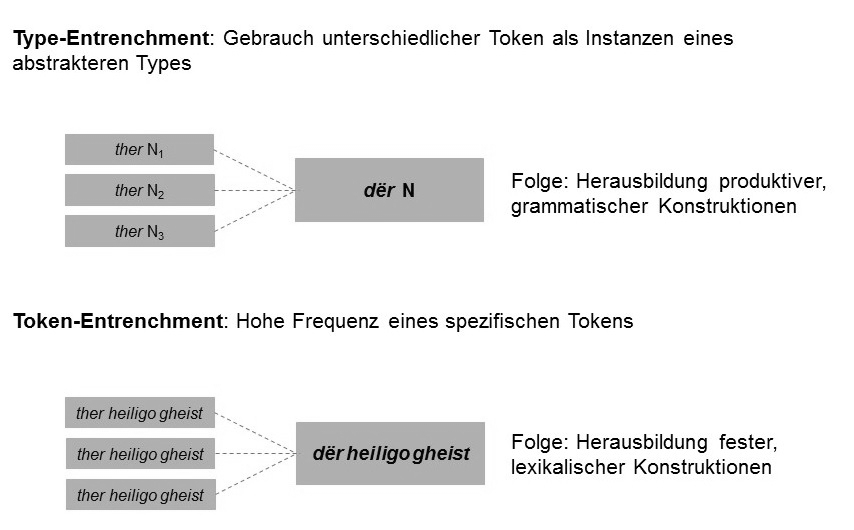
\includegraphics[width=12cm]{images/type-token-entrenchment-neu-sw.jpg}
  \fbox{\begin{minipage}{.985\textwidth}\raggedright
  \emph{Type-Entrenchment}: Gebrauch unterschiedlicher Token als Instanzen eines abstrakten Types\\
  \begin{center}
  \begin{forest} for tree={edge={dotted,thick}}
  [\textit{dër} N,grow=west,l sep=1cm
    [\textit{ther} N\textsubscript{1}]
    [\textit{ther} N\textsubscript{2}]
    [\textit{ther} N\textsubscript{3}]
  ]
  \end{forest}\hspace{1em}\parbox[t]{.5\textwidth}{\raggedright Folge: Herausbildung produktiver, grammatischer Konstruktionen}\\
  \end{center}
  \emph{Token-Entrenchment}: Hohe Frequenz eines spezifischen Tokens\\
  \begin{center}
  \begin{forest} for tree={edge={dotted,thick}}
  [\textit{dër heiligo gheist},grow=west,l sep=1cm
    [\textit{ther heiligo gheist}]
    [\textit{ther heiligo gheist}]
    [\textit{ther heiligo gheist}]
  ]
  \end{forest}\hspace{1em}\parbox[t]{.4\textwidth}{\raggedright Folge: Herausbildung fester, lexikalischer Konstruktionen}\\
  \end{center}
  \end{minipage}}
\caption {Type- und Token-Entrenchment} 
\label{abb:type-token-entrechment}
\end{figure} 

Indirekt kann allerdings auch Token-Entrenchment die Ausbildung von schematischen Konstruktionen beeinflussen. So geht bspw. \textcite[96]{Bybee2010} davon aus, dass spezifische Konstruktionen Vorbild für parallel strukturierte Ausdrücke sein können und damit eine Schematisierung ankurbeln. Sie demonstriert am Beispiel der spanischen Konstruktion \is{Konstruktion}  \object{quedarse}\,+\,Adjektiv, dass die generellere, schematische  Konstruktion \is{Konstruktion}  über analogische Prozesse \is{Analogie} aus einem einzelnen Vorbild (dem Typ \object{quedarse sólo}) entstanden ist \parencite[72]{Bybee2010}. In Bezug auf die Herausbildung von [Definitartikel\,+\,N] kann man postulieren, dass frühe Kollokationen mit \object{dër} sich positiv auf den funktionalen Wandel von Demonstrativ- \is{Demonstrativartikel} zu \isi{Definitartikel} auswirken. So ist bspw. aus der Untersuchung von \textcite{Oubouzar1992} bekannt, dass eindeutig identifizierbare Referenten wie  z.B. \object{heilant} als Übersetzung von \object{Iesus} (im Tatian) auffallend häufig mit \object{dër} determiniert werden. Da eine zusätzliche situative Verortung bzw. ein demonstrativer Verweis in diesen Fällen nicht der Grund für die Determinierung sein kann, liegen hier semantisch-definite (situationsunabhängige) Gebrauchskontexte vor, d.h. Kontexte, die ausschließlich dem \isi{Definitartikel} vorbehalten sind (s. hierzu ausführlich Kapitel \ref{sec:definitartikel}). Kollokationen dieser Art können damit als frühe Instanzen der Konstruktion \is{Konstruktion}  [Definitartikel + N] gewertet werden. \textcite[96]{Bybee2010} zufolge ist die immer noch vorhandene strukturelle Transparenz solcher Token die Voraussetzung, dass Analogieprozesse \is{Analogie} stattfinden.   

Möglich ist auch, dass unterschiedliche Konstruktionen miteinander um ihren Platz im kog"-ni"-ti"-ven Netzwerk konkurrieren und so bestimmte Entrenchment-Formen einander blockieren. Dies ist im Deutschen -- ebenso wie in anderen germanischen Sprachen \parencite[s.][]{Himmelmann1998} -- bei adverbial \is{Adverbial}
 gebrauchten Präpositionalphrasen zu beobachten. Als Teil eines Adverbials \is{Adverbial} kann ein Nomen nämlich undeterminiert bleiben, während es in Argumentpositionen ein Artikelwort braucht, vgl. \exref{ex:fuss}. Wie in Abschnitt (\ref{sec:partizipanten}) noch gezeigt wird, lässt sich diese Form der Artikellosigkeit auch mit der Partizipantenrolle \is{Semantische Rolle}
 (hier: Patiens vs. Instrument) und der damit zusammenhängenden Nicht-Referentialität \is{Referentialität} erklären.  

\begin{exe}
	\ex \label{ex:fuss}
	\begin{xlist}
		\ex \label{ex:denfuss} \object{Er hält sich den Fuß.} (Objekt) \is{Objekt} 
		\ex \label{ex:zufuss} \object{Er läuft zu Fuß.} (Adverbial) \is{Adverbial}
	\end{xlist}
\end{exe}

Auch im Ahd. sind es insbesondere die in PPs eingebetteten Nomen, die sich einer Determinierung mit \object{dër} entziehen, z.B. \object{in himile} \extrans{im Himmel} oder \object{fone uuinde} \extrans{vom Winde} \parencite[84]{Oubouzar1992}; s. hierzu auch Abschnitt \ref{sec:extension}. Es scheint, als ob die Konstruktion \is{Konstruktion}  [Präp\,+\,N] so stark entrenched wurde, dass sie die emergierende Konstruktion \is{Konstruktion} [Definitartikel\,+\,N] überlagert. Phrasen ohne Artikel werden auf diese Weise syntaktisch konserviert. Je stärker der Entrenchmentgrad, umso resistenter ist die Konstruktion \is{Konstruktion}  gegenüber phonologischen oder morphosyntaktischen Veränderungen, denen verwandte Strukturen unterworfen sind \parencite[715]{Bybee2006}. So können sich bestimmte Types des Musters [Präp\,+\,N] bis heute zu einer eigenständigen und nicht-kompositionellen \isi{Konstruktion} entwi"ckelt haben \parencite[343--344]{Himmelmann1998}. 

Entrenchment als kognitives Prinzip bedingt die Entwicklung einer grammatischen \isi{Konstruktion}  also aus mehreren Richtungen. Es ist zum einen der Grundmechanismus für die erfolgreiche produktive Verwendung und damit der Extension eines Schemas, etwa [\object{dër}\,+\,N] oder [Präp\,+\,N]. Zum anderen kann Entrenchment dafür sorgen, dass bestimmte Token nicht-kompositionelle Eigenschaften ausbilden. Dies ist der Fall, wenn \object{dër} in bestimmten Kollokationen bereits einen Funktionswandel von Demonstrativ- \is{Demonstrativartikel} zu \isi{Definitartikel} erfahren hat und dann in dieser Bedeutung analogisch \is{Analogie} auch mit neuen Appellativa gebraucht wird. 


\section{Mechanismen des Wandels}\label{sec:mechanismen}

Wenn eine neue \isi{Konstruktion}  entsteht, sind typischerweise zwei Wandelmechanismen am Werk: Vereinfacht ausgedrückt, sorgt die \isi{Analogie} für die graduelle Kontextextension, während die \isi{Reanalyse} für den Bedeutungs- und Strukturwandel zuständig ist. In der Gram"-mati"-ka"-li"-sierungs- und \is{Grammatikalisierung} daran anknüpfend  Konstruktionalisierungsforschung \is{Konstruktionalisierung} gibt es eine rege Diskussion um den Stellenwert dieser Mechanismen \parencite[vgl. u.a.][]{Haspelmath1998,Lehmann2004,Fischer2007}. In der vorliegenden Arbeit wird davon ausgegangen, dass der \isi{Definitartikel} das Resultat aus einer Kombination aus beidem ist --  \isi{Analogie} und \isi{Reanalyse} -- und sich die Mechanismen, wie in den nachfolgenden Abschnitten gezeigt wird, gegenseitig bedingen. Sie sind durch zwei unterschiedliche kognitive Strategien motiviert: Der \isi{Analogie} liegt das analogische Denken \is{Analogie} zugrunde, die \isi{Reanalyse} beruht auf dem syntaktischen Parsen des sprachlichen Inputs \parencite[38]{Traugott2013}.  


\subsection{Analogie}\label{sec:analogie}

Eine \isi{Analogie} liegt vor, wenn ein sprachlicher Ausdruck nach dem Vorbild eines bestimmten Musters (nach-)gebildet wird. So kann es z.B. innerhalb eines Flexionsparadigmas zu formalen Angleichungen kommen (=\,analogischer Ausgleich). Ein prominentes Beispiel aus der deutschen Sprachgeschichte ist die frnhd. Numerusprofilierung \parencite[1543]{Wegera2000a}, bei der die kasusmarkierenden \object{n}-Endungen der schwachen Feminina im Akkusativ, Dativ und Genitiv Singular getilgt werden und auf diese Weise Singular und Plural intraparadigmatisch formal ausdifferenzieren, s. Abbildung~\ref{abb:zunge}. Das Vorbild für die \isi{Analogie} ist der Nominativ Singular \object{zunge}. 

\begin{figure}
% %   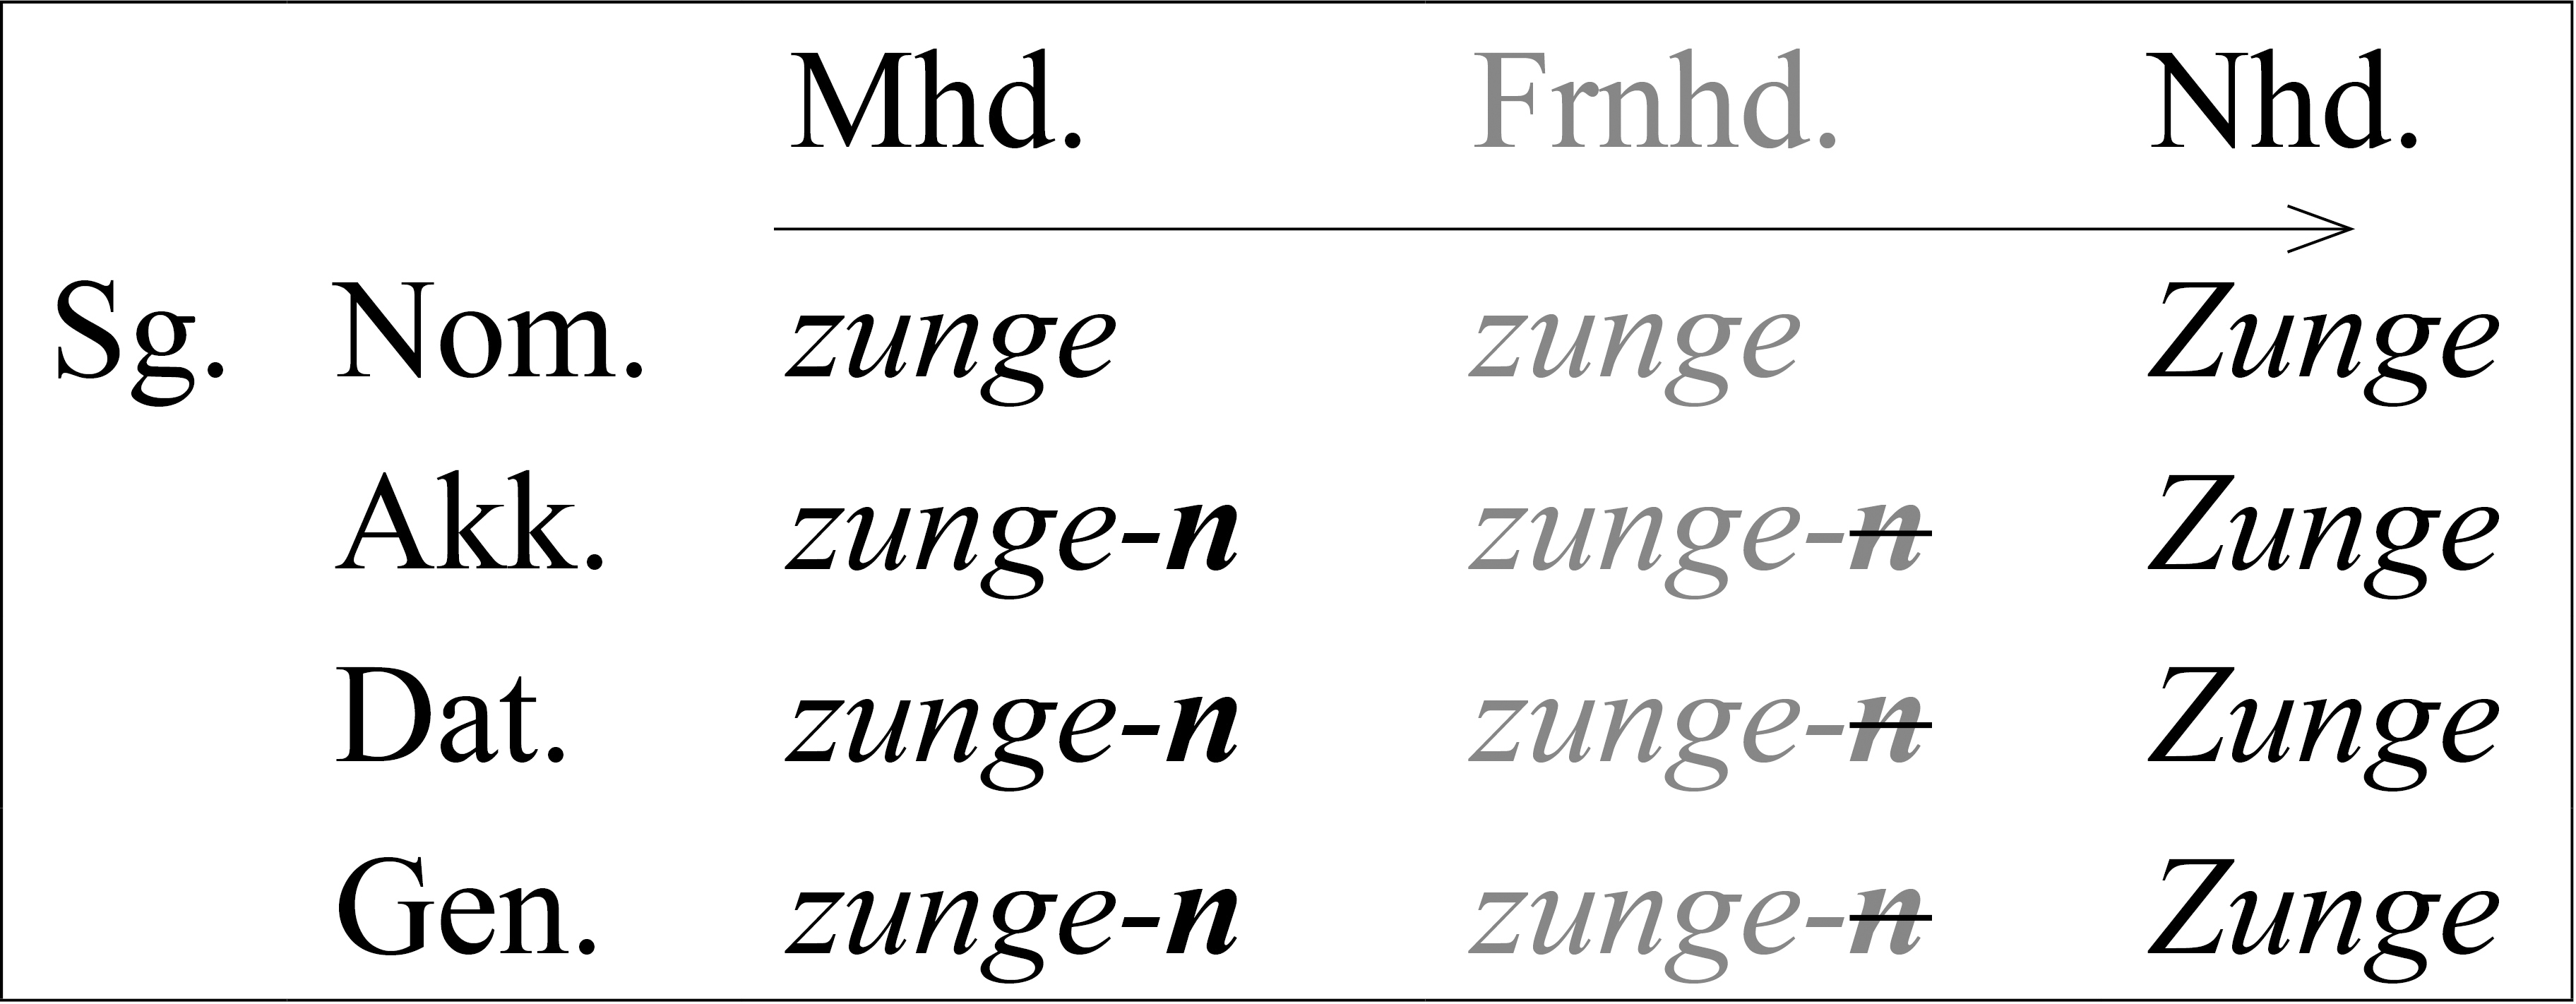
\includegraphics[width=7cm]{images/zunge.jpg}
  \begin{tabular}{ll>{\itshape}l>{\color{lsGuidelinesGray}\itshape}l>{\itshape}l}
  & & \tikzmark{Wegeramhd}\normalfont Mhd. & \upshape Frnhd. & \normalfont Nhd.\\\tablevspace
  Sg. & Nom. & zunge & zunge & Zunge\\
      & Akk. & zunge-\textbf{n} & zunge-\sout{\textbf{n}} & Zunge\\
      & Dat. & zunge-\textbf{n} & zunge-\sout{\textbf{n}} & Zunge\\
      & Gen. & zunge-\textbf{n} & zunge-\sout{\textbf{n}} & Zunge\\
  \end{tabular}
  \begin{tikzpicture}[overlay,remember picture]
  \draw[-{Triangle[]}] (pic cs:Wegeramhd)+(0,-.166) -- ++(3.8cm,-.166);
  \end{tikzpicture}
\caption {Analogischer Ausgleich bei \object{Zunge}, entnommen aus \textcite[24]{Wegera2012}\label{abb:zunge}}
\end{figure} 

\textcite[160]{Lehmann2004} führt ganz ähnliche Fälle des analogischen Ausgleichs an, wenn er über die Rolle der \isi{Analogie} bei der \isi{Grammatikalisierung} spricht.\footnote{Er illustriert die \isi{Analogie} mit dem  Wandel von starker zur schwacher Flexion bei den Maskulina: mhd. \object{der hane, des hanen, die hanen} zu frnhd. \object{der Hahn, des Hahns, der Hähne}.} Seiner Meinung nach kommt die Entwicklung von Definitartikeln ganz ohne \isi{Analogie} aus, da es kein vergleichbares formales Muster gebe, das die \isi{Grammatikalisierung}  antreibe; ein analogischer Ausgleich \is{Analogie} finde also nicht statt. Lehmann sieht die Artikelentwicklung deswegen als Beweis für die Existenz von \blockcquote[161]{Lehmann2004}{pure grammaticalization without analogy}. 

Wenn man Analogien \is{Analogie} lediglich innerhalb von Flexionsparadigmen sucht, ist diese Sicht vielleicht gerechtfertigt. Analogische Prozesse \isi{Analogie} reichen allerdings weit über die intraparadigmatischen Grenzen hinaus: Aus gebrauchsbasierter Sicht gleichen Sprecherinnen und Sprecher den Input, den sie bekommen, unentwegt mit bestehenden Konstruktionen in ihrem mentalen Netzwerk ab. Auf diese Weise kann ein existierendes Schema z.B. neue Mitglieder akquirieren. Ein prominentes Beispiel hierfür ist die Bildung von ehemals starken Verben nach dem Muster der schwachen Flexion, z.B. mhd. \object{bellen > ball} > nhd. \object{bellen > bellte} \parencite{Bittner1985}. \isi{Analogie} ist dann gleichzusetzen mit der graduellen Ausbreitung einer \isi{Konstruktion}  auf neue Kontexte \parencite[57--58]{Bybee2010}. % Lehmann bezeichnet diesen Sprachwandel als \blockcquote[162]{Lehmann2004}{analogically-oriented grammaticalization}. 

Auch wenn kein direkt sichtbares Vorbild existiert, nach der die \isi{Konstruktion}  [Definitartikel\,+\,N] gebildet wird, so sind es dennoch analogische \is{Analogie}  Prozesse, die dem  Wandel von Demonstrativ- \is{Demonstrativartikel} zu \isi{Definitartikel} zugrunde liegen \parencite[eine ähnliche Perspektive nimmt auch Sommerer bei der Entwicklung des engl. Definitartikels ein, s.][]{Sommerer2011}. Denn sprachliche Innovationen werden von Sprecherinnen und Sprechern stets mit existierenden Knoten abgeglichen, die formal oder funktional Ähnlichkeiten aufweisen \parencite[51]{Traugott2013}. Kleinste formale und/oder funktionale Unterschiede\footnote{Langacker zufolge ist ein \blockcquote[69]{Langacker1987}{considerable amount of nonconventionality [...] tolerated (and often expected) as a normal feature of language use}.}
 können dabei Veränderungen im Konstruktionsnetzwerk bewirken:  \blockcquote[324]{Fischer2007} {The perception of similarity, or perhaps better the inability to see a difference […] between two linguistic signs or between two referents, may cause the learner/speaker to shift such an element to another set in his processing system, a set that is functionally or formally close.} Jeder innovative Gebrauch von [\object{dër}\,+\,N] veranlasst den Adressaten also, einen Abgleich mit bekannten und ähnlichen \object{chunks} \parencite[60]{Bybee2010} im mentalen Netzwerk vorzunehmen und ggf. die Verbindungen neu zu justieren. Wenn \object{dër} wiederholt in Kontexten gebraucht wird, die nicht dem prototypischen Arbeitsbereich von Demonstrativa \is{Demonstrativum} entsprechen, kann dies langfristig das Verhältnis von Form und Funktion verändern und zur Ausbildung eines neuen Schemas (vgl. Abschnitt \ref{sec:schema}) führen, das wiederum auf neue Instanzen analogisch \is{Analogie} übertragen werden kann. Konkret heißt dies, dass die demonstrative Information mit wiederholtem Gebrauch nach und nach in den Hintergrund rückt und \object{dër} als bloßer Definitheitsmarker \isi{Definitheit} reanalysiert \is{Reanalyse} wird.

\subsection{Reanalyse}\label{sec:reanalyse}

Unter \isi{Reanalyse} versteht man die Um- oder Neuinterpretation\footnote{Zur Diskussion um den Vorschlag einer terminologischen Neuetikettierung von \isi{Reanalyse} zu \object{Neoanalyse} s.  \textcite[36]{Traugott2013}.} einer sprachlichen Struktur. In dieser recht weiten Definition wurde der Begriff in den vorherigen Abschnitten bereits genutzt. Vertreter eines engeren Reanalysekonzepts \is{Reanalyse} wie bspw. \textcite[215]{Heine1991} gehen davon aus, dass mit der Uminterpretation immer eine Neudefinition der Konstituentengrenzen einhergeht: \blockcquote[216]{Heine1991}{[...] we confine ourselves to what [...] is called constituent-internal reanalysis, the specific form of the more general process of reanalysis, which has the effect of redefining constituent boundaries}. Bei der \isi{Grammatikalisierung} des Definitartikels sei vor diesem Hintergrund keine \isi{Reanalyse}  beteiligt, da sowohl dem Demonstrativ- \is{Demonstrativartikel} wie dem \isi{Definitartikel} gleichermaßen der Kopfstatus in der Phrase zukäme und sich syntaktisch nichts veränderte \parencite[219]{Heine1991}. Auch in der generativen Grammatik wird die \isi{Reanalyse} als Wandelmechanismus begriffen, der die hierarchischen Verhältnisse im Satz bzw. in der Phrase beeinflusst: Das \isi{Demonstrativum}, welches ursprünglich die \object{Spec-Position} einnimmt, wird im Zuge der \isi{Grammatikalisierung} zum Kopf der NP bzw. DP erhoben. Daher betrachten Vertreterinnen dieser Theorie die Herausbildung des Definitartikels als eindeutigen Fall einer syntaktischen \isi{Reanalyse} \parencite[vgl. bspw.][]{Philippi1997,vanGelderen2007}.\footnote{Zur Frage, ob das Artikelwort oder das Nomen den Kopf der Phrase bildet, s. ausführlich \textcite[145--146]{Himmelmann1997}.}

In der vorliegenden Arbeit wird \isi{Reanalyse} als kategorialer Wandel von De"-mon"-strativ- zu \isi{Definitartikel} aufgefasst, der weitere Grammatikalisierungsprozesse \is{Grammatikalisierung} (etwa die Obligatorisierung des Artikelwortes) nach sich zieht. Die \isi{Reanalyse} ist ein Prozess, der formseitig zunächst unsichtbar bleibt \parencite[58]{Langacker1977}. Erst durch die analogische \is{Analogie} Ausweitung der neuen Struktur auf neue Kontexte werden kategoriale Verschiebungen sichtbar. \textcite[50]{Hopper2006} illustrieren dies an einem Beispiel aus der Lexik: Erst die Substitution von \object{ham} durch \object{cheese} legt offen, dass das Lexem \object{hamburger} eine neue Lesart erhalten hat \parencite[urspr. \extrans{Hamburg(er) Steak}][389]{Kluge2011}. Ein aktuelles Beispiel für eine \isi{Reanalyse} auf Mehrwortebene ist die Entstehung des Rezipientenpassivs, bei dem ein adjektivisches Partizip verbal gedeutet wird, wie in \object{Ich bekomme den Kaffee geröstet} \parencite[152--153]{Szczepaniak2011a}.
 %oder \object{Sie hat die Daten annotiert}
Die Voraussetzung für die \isi{Reanalyse} sind also sprachliche Bausteine, die in bestimmten Kontexten ambig sind. Kategoriale \hervor{Zwitter} wie Partizipien oder Infinitive \parencite[vgl. die \isi{Reanalyse} des \object{am}-Progressivs: Aus einem nominalen wird ein verbaler Infinitiv, s.][]{Flick2013} sind prädestiniert dafür, Ambiguitäten auszulösen. 

Im Vergleich dazu läuft die \isi{Reanalyse} des Definitartikels anders ab. Denn hier ist in der Spenderkonstruktion \is{Konstruktion}  zunächst keine Mehrdeutigkeit angelegt: Am Anfang steht \hervor{nur} ein adnominales Demonstrativ. Es gibt keinen Kontext, in dem eine andere Wortart oder eine andere syntaktische Analyse möglich wäre. Um eine \isi{Reanalyse} einzuleiten, muss es das \isi{Demonstrativum} in ungewöhnlichen Kontexten zum Einsatz kommen und dieser neue Gebrauch muss dann eine alternative Lesart zulassen. Wie in Abschnitt \ref{sec:kata} noch ausführlich dargelegt wird, kann man davon ausgehen, dass die Innovation, die dem Startschuss in Richtung \isi{Definitartikel} entsprach, darin lag, dass das \isi{Demonstrativum} \object{dër} gebraucht wurde, um wichtige Referenten im Diskurs zu exponieren. Immer mehr Sprecherinnen und Sprecher imitieren diese neue diskurs"-strukturierende Maßnahme, was zur allmählichen Routinisierung und Abschwächung der Hervorhebungsfunktion führt. Die Struktur [\object{dër}\,+\,N] etabliert sich auf dem Weg dorthin als neues Schema: Aus einem fakultativ gebrauchten \isi{Demonstrativum} wird ein obligatorisch zu setzender Definitartikel. Die \isi{Reanalyse} läuft hierbei in vielen kleinen Mikroschritten ab, indem Sprecherinnen und Sprecher den sprachlichen Input immer wieder mit bestehenden Konstruktionen abgleichen und diese anpassen, was langfristig einen graduellen Wandel auf Systemebene zur Folge hat.\footnote{Zur Diskussion, inwiefern \isi{Reanalyse} abrupt oder graduell verläuft s. die Übersicht in \textcite[75]{Traugott2013}. In Bezug auf die Entwicklung des Definitartikels plädiert insbesondere \textcite{Schlachter2015} für eine abrupte \isi{Reanalyse}.} 
Dadurch wird mit jedem neuen und etwas unüblicheren Gebrauch die ursprüngliche Bedeutung von [\object{dër}\,+\,N] sozusagen überschrieben: Aus einer Demonstrativkonstruktion \is{Konstruktion}  entwickelt sich eine Definitartikelkonstruktion.

  
\section{Zusammenfassung}

Der deutsche \isi{Definitartikel} hat sich aus dem adnominal gebrauchten \isi{Demonstrativum} \object{dër} herausgebildet. Diese Entwicklung entspricht den frühen Stufen der von \textcite{Greenberg1978} und \textcite{Lehmann2015} beschriebenen, universellen Grammatikalisierungspfade \is{Grammatikalisierungspfad} für Definitartikel, welche von \textcite{Schmuck2014} für das Althochdeutsche konkretisiert wurden. Die vorliegende Arbeit setzt sich zum Ziel, diesen Pfad mithilfe einer Korpusuntersuchung nachzuzeichnen und, wenn notwendig, neu zu modellieren. Die Entwicklung  des Definitartikels ist einerseits ein Musterbeispiel für Grammatikalisierung, da die für diesen Sprachwandeltyp typischen Prozesse (u.a. Obligatorisierung, semantische und formale Reduktion)  durchlaufen werden. Dass am Anfang des Wandels kein lexikalisches Morphem steht, wird in der Forschung hingegen als Besonderheit hervorgehoben. Das \isi{Demonstrativum} leistet jedoch funktional viel mehr als andere grammatische Morpheme (etwa Präpositionen). Deswegen verwundert es nicht, dass es als Quelle für Grammatikalisierungen fungiert; in Abschnitt \ref{sec:kata} wird auf diesen Aspekt noch ausführlich eingegangen. Die Erkenntnisse aus der \isi{Grammatikalisierung} sind mit einer konstruktionsgrammatischen und gebrauchsbasierten Sprachauffassung gut vereinbar. Vor diesem Hintergrund kann die Entwicklung des Definitartikels als \isi{Konstruktionalisierung} betrachtet werden: Hierbei entsteht aus [Demonstrativartikel\,+\,N] die Konstruktion \is{Konstruktion}  [Definitartikel + N] mit der Bedeutung, Referenten als eindeutig identifizierbar zu kennzeichnen. Gleichzeitig wandeln sich die Relationen im NP-Netzwerk. Durch Entrenchment-Prozesse entstehen neue Knoten, darunter das abstrakte Determiniererschema, das die Ausbreitung von \object{dër} stützt. Als zentrale Mechanismen hinter dem Wandel wurden die \isi{Analogie} und die \isi{Reanalyse} herausgearbeitet. Erstere sorgt dafür, dass [\object{dër} + N] in neuen Kontexten gebraucht wird, letztere bewirkt die neue Lesart (Definit- statt Demonstrativartikel). 

%\chapter{Von einer artikellosen Sprache zu einer Artikelsprache}\label{forschung}


Mit der Entwicklung des Definitartikels wandelt sich das Deutsche in wenigen Jahrhunderten, nämlich im Laufe der ahd. Sprachperiode,  von einer artikellosen Sprache zu einer Artikelsprache. 
In diesem Kapitel wird dieser Wandel vor dem Hintergrund der aktuellen Forschung diskutiert. Abschnitt \ref{sec:def-ahd} geht der Frage nach, welche Möglichkeiten das Althochdeutsche kannte, um Definitheit -- trotz des Fehlens eines Definitartikels -- auszudrücken. Während sich die Forschung darüber einig ist, dass der Definitartikel seinen Ursprung im ahd. Demonstrativum \object{dër} hat,
gibt es auf die Frage nach den Ursachen der Entwicklung ganz unterschiedliche Antworten. Diese werden in Abschnitt \ref{sec:gruende} vorgestellt und kritisch beleuchtet. Dabei ist allen bisherigen Entstehungstheorien gemein, dass die Herausbildung des Definitartikels ein Ausgleich für bestimmte Defizite im ahd. Sprachsystem sein soll. In Abschnitt \ref{sec:demzudef} wird diese Auffassung problematisiert und ein Perspektivenwechsel vorgenommen, indem das Demonstrativum  in seiner Funktion, Referenten als diskursprominent zu markieren, in den Blick genommen wird. 

\section{Definitheit im Althochdeutschen} \label{sec:def-ahd}

Definitheit ist eine universelle Kategorie \parencite[269]{Leiss2000}. Sprachen, die Definitheit nicht in Form eines Definitartikels ausdrücken, nutzen alternative Strategien, um Referenten als definit zu kennzeichnen \parencite[für einen typologischen Überblick s.][]{Kramsky1972}. Das (frühe) artikellose Althochdeutsche greift ebenfalls auf verschiedene syntaktische und morphologische Mittel zurück, um definite Interpretationen zu erzielen. Sie werden in diesem Abschnitt vorgestellt.\footnote{Einführende Zusammenfassungen zum Ausdruck von Definitheit im Althochdeutschen bieten \textcite{Szczepaniak2011a}, \textcite{Ferraresi2014} und \textcite{Szczepaniak2015}.}

\subsection{Determinierer}\label{determinierer}

Neben dem sich entwickelnden Definitartikel \object{dër} verfügt das Althochdeutsche über eine Reihe von Determinierern, die zur eindeutigen Identifikation eines Referenten beitragen und somit Definitheit zum Ausdruck bringen.
Auf Basis althochdeutscher Grammatiken \parencite{, Meineke2001, Sonderegger2003,Braune2004} kann man die folgenden Gruppen unterscheiden:  

\begin{enumerate}[label=\alph*)]
		\item \label{poss} Possessiva: \object{m\={i}n, d\={i}n, s\={i}n} etc.
		\item \label{dieser} Demonstrativa: \object{dër, dëser, jener, solih/solicher, sëlb, der samo}
\end{enumerate}

Possessiva und Demonstrativa haben gemein, dass es nicht zu ihrer Hauptfunktion gehört, Definitheit anzuzeigen, sondern sich diese quasi als Nebeneffekt aufgrund von anderen Bedeutungskomponenten ergibt: So drückt ein Possessivum typischerweise ein Besitzverhältnis aus (\object{mein Buch, meins}). Der eindeutige Bezug von Possessor und Possessum löst eine Definitheitsinterpretation aus \parencite[332]{Hoffmann2009}. Das zusammengesetzte Demonstrativum \object{dëser}\footnote{Bei der Form handelt sich um die Verbindung aus \object{dër} und der Partikel \object{se} (< *\object{sa}, \object{si}), vgl. \textcite[260]{Meineke2001}.} (nhd. \object{dieser}) wird nach \textcite[164]{Oubouzar1997a} für den unmittelbaren anaphorischen Verweis gebraucht. Die definite Lesart ist also Ergebnis der kontextuell bedingten Koreferenz. Auch die Demonstrativa \object{jener},  \object{sëlb} und \object{solih} wirken determinierend, indem sie auf etwas Vorerwähntes und somit Bekanntes verweisen.\footnote{Zur Abgrenzung von \object{solch} gegenüber anderen Determinierern s. \textcite{Demske2005}.} Sie alle haben zusätzlich das Potential, auf eine Entität in der unmittelbaren Umgebung zu referieren (vgl. den sog. situativen Gebrauch in Abschnitt \ref{sec:situativ}) und damit für eine definite Abgrenzung zu sorgen. 

\textcite[32ff.]{Lyons1999} nennt neben Possessiva und Demonstrativa für das Englische noch die   Quantifizierer \object{all, both, every} und \object{most} als adnominale Definitheitsausdrücke, deren Äquivalente auch im Althochdeutschen existieren. Während die ersten drei aus Lyons Liste jeweils auf die Totalität einer bestimmten Menge verweisen und damit die Identifizierbarkeit gewährleisten \parencite[vgl. auch][334]{Hoffmann2009}, beschreibt \object{most} ähnlich wie \object{all} eine \blockcquote[33]{Lyons1999}{proportion of some whole -- as indeed does \object{the} if it is inclusive}. Sie leisten also in bestimmten Kontexten das Gleiche wie der Definitartikel. 
Darüber hinaus kann man auch mit Ordinalzahlen einen eindeutigen Verweis erwirken, da die Identifikation durch eine klar definierte Position in einer bestimmten Rangordnung erfolgt, z.B. \object{der erste/zweite} aus einer bestimmten (vorerwähnten) Gruppe. Im Gegenwartsdeutschen treten Ordinalzahlen daher zusammen mit Definitartikeln auf.

In Opposition zu diesen definiten Determinierern kennt das Althochdeutsche zudem auch artikelartige Wörter, die Indefinitheit zum Ausdruck bringen \parencite[253-254]{Braune2004}, etwa das Indefinitpronomen \object{sum} \parencite{Donhauser2012} oder das Zahlwort \object{ein} -- der Vorläufer des heutigen Indefinitartikels \parencite{Oubouzar2000,Szczepaniak2016}. 

Was das Stellungs- und Kombinationsverhalten betrifft, ist das Althochdeutsche  flexibler als das Gegenwartsdeutsche \parencite[104]{Szczepaniak2011a}. So können Possessiva beispielsweise sowohl voran- als auch nachgestellt werden und auch in Kombination mit anderen Determinierern auftreten, s. \REF{ex:poss-stellung}; Beispiele aus \textcite[27-28]{Schrodt2004}.\footnote{Zum syntaktischen Status der Possessiva im Althochdeutschen s. \textcite[132ff.]{Demske2001}.} Die Studie von \textcite{Flick2018} zum ahd. Isidor deutet allerdings darauf hin, dass sowohl bei Possessiva als auch bei Demonstrativa schon im frühen Althochdeutschen die Voranstellung überwiegt.

\begin{exe}
	\ex \label{ex:poss-stellung}   
	\begin{xlist}
		\ex \label{ex:possvor} Pränominales Possessivum: \object{sinen brouder} \extrans{seinen Bruder}
		\ex \label{ex:possnach} Postnominales Possessivum: \object{chuning min} \extrans{mein König} 
		\ex \label{ex:posskombi} Kombination mit \object{dër}: \object{thaz min kind} \extrans{das mein Kind}
		\end{xlist}
\end{exe}


Für die vorliegende Arbeit ist das System der Determinierer im Althochdeutschen  vor allem aus zwei Gründen relevant: Erstens soll die Frage beantwortet werden, wie sich der emergierende definite Artikel in das System eingliedert und bestehende Distributionen verändert. Zweitens soll über die Analyse der Nominalsyntax herausgefunden werden, inwiefern sich ein Determiniererschema herausgebildet hat, in welchem der Definitartikel als Teil einer neuen Konstruktion [Definitartikel\,+\,Nomen] grammatikalisiert bzw. konstruktionalisiert wird (vgl. hierzu die Ausführungen in Abschnitt \ref{sec:schema}). 

\subsection{Schwache Adjektivflexion} \label{schwache-Adjektivflexion}

Attributiv gebrauchte Adjektive stellen eine weitere Möglichkeit dar, um im Althochdeutschen Definitheit zu markieren. So können schwach flektierte Adjektive -- in Opposition zu stark flektierten Formen -- für eine Individualisierung des Referenten sorgen \parencite[68]{Szczepaniak2011a}. Die starke Flexion bewirkt eine indefinite Lesart, vgl. Tabelle \ref{tab:schwach-adj} und \ref{tab:stark-adj}.  Weil die schwache Flexion dem Paradigma der substantivischen \object{an-} und \object{on-}Stämme folgt, wird sie auch als nominale Deklination bezeichnet -- im Gegensatz zur pronominalen  (durch die Flexion der Pronomina beeinflussten) starken Flexion \parencite[s.][251]{Meineke2001}. 

\begin{table}

\begin{tabular}{lllll}
\lsptoprule
                  &               & \multicolumn{1}{l}{{Maskulinum}}  & \multicolumn{1}{l}{{Neutrum}}     & \multicolumn{1}{l}{{Femininum}}       \\ \midrule
{Sg.} & {Nom.} & \textit{blinto}                          & \textit{blinta}                          & \textit{blinta}                              \\
                  & {Gen.} & \textit{blinten, -in}                    & \textit{blinten, -in}                    & \textit{blintun}                             \\
                  & {Dat.} & \textit{blinten, -in}                    & \textit{blinten, -in}                    & \textit{blintun}                             \\
                  & {Akk.} & \textit{blinton, -un}                    & \textit{blinta}                          & \textit{blintun}                             \\
{Pl.}   & {Nom.} & \textit{blinton, -un}                    & \textit{blintun, -on}                    & \textit{blintun}                             \\
                  & {Gen.} & \textit{blintono}                        & \textit{blintono}                        & \textit{blintono}                            \\
                  & {Dat.} & \textit{blintom, -on}                    & \textit{blintom, -on}                    & \textit{blintom, -on}                        \\
                  & {Akk.} & \textit{blinton, -un}                    & \textit{blintun, -on}                    & \textit{blintun}                             \\\midrule
                  & {Bsp.} & \multicolumn{1}{l}{\textit{blinto gast}} & \multicolumn{1}{l}{\textit{blinta lamb}} & \multicolumn{1}{l}{\textit{blinta kuningin}} \\
                  & {Nhd.}          & \multicolumn{1}{l}{der blinde Gast}      & \multicolumn{1}{l}{das blinde Lamm}      & \multicolumn{1}{l}{die blinde Königin}       \\ \lspbottomrule
\end{tabular}
\caption{Schwache Adjektivdeklination [+individualisierend] am Beispiel von \herkur{blinto} \extrans{blind} \parencite[226]{Braune2004}}
\label{tab:schwach-adj}
\end{table}

\begin{table}
\resizebox{\textwidth}{!}{\begin{tabular}{lllll}
\lsptoprule
{}         & {}              & \multicolumn{1}{l}{{Maskulinum}} & \multicolumn{1}{l}{{Neutrum}} & \multicolumn{1}{l}{{Femininum}} \\ \midrule
{Sg.} & {Nom.}          & \textit{blint/blinter}                  & \textit{blint/blintaz}               & \textit{blint/blint(i)u}               \\
{}         & {Gen.}          & \textit{blintes}                        & \textit{blintes}                     & \textit{blintera}                      \\
{}         & {Dat.}          & \textit{blintemu, -emo (amu)}           & \textit{blintemu, -emo (amu)}        & \textit{blintera}                      \\
{}         & {Akk.}          & \textit{blintan}                        & \textit{blint/blintaz}               & \textit{blinteru, -ero}                \\
{Pl.}   & {Nom.}          & \textit{blinte/blint}                   & \textit{blintiu/blint}               & \textit{blinto/blint}                  \\
{}         & {Gen.}          & \textit{blintero}                       & \textit{blintero}                    & \textit{blintero}                      \\
{}         & {Dat.}          & \textit{blintem, -en}                   & \textit{blintem, -en}                & \textit{blintem, -en}                  \\
{}         & {Akk.}          & \textit{blinte}                         & \textit{blint(i)u}                   & \textit{blinto}                        \\\midrule
                  & {Bsp.} & \textit{blint gast}                     & \textit{blint lamb}                  & \textit{blint kuningin}               \\
                  & {Nhd.}          & ein blinder Gast                        & ein blindes Lamm                     & eine blinde Königin                     \\ \lspbottomrule
\end{tabular}}
\caption{Starke Adjektivdeklination [\textminus{}individualisierend] am Beispiel von \herkur{blint} \extrans{blind} \parencite[220]{Braune2004}}
\label{tab:stark-adj}
\end{table}


\textcite[361ff.]{Braunmuller2008} zufolge soll es sich bei der schwachen (und jüngeren) Adjektivflexion ursprünglich um ein Wortbildungsmuster gehandelt haben, das Sprecherinnen und Sprecher als Folge von Sprachkontakt als Flexiv reanalysierten \parencite[zu alternativen Entstehungsszenarien s.][13--26]{Kovari1984}. Vermutlich konnte ein schwach flektiertes Adjektiv in voralthochdeutscher Zeit selbstständig Definitheit am Bezugsnomen anzeigen 
\parencites()()[69]{Demske2001}[364]{Braunmuller2008}. Noch im ahd. Isidor finden sich Beispiele für diese selbstständige Definitheitsmarkierung, etwa \object{himiliscun got} \extrans{den himmlischen Gott} (I 7,1) \parencite[226]{Braune2004}; s. auch \textcite[69-70]{Demske2001}. 
Viel häufiger erhalten schwach deklinierte Adjektive im Althochdeutschen allerdings schon funktionale Unterstützung vom emergierenden Definitartikel, vgl. beispielhaft die Belege in \REF{ex:art-adj} aus \textcite[24,28]{Schrodt2004}, was zur einer allmählichen Routinisierung des Musters [\object{dër}\,+\,Adjektiv\,+\,Nomen] führt (s. hierzu auch Abschnitt \ref{ersatz-schwach}).

\begin{exe}
	\ex \label{ex:art-adj}   
	\begin{xlist}
		\ex \label{ex:art-adj1} \object{mit dheru smelerun dheidu} \\   \extrans{mit dem geringerem Volk} (I 9,9) 
		\ex \label{ex:art-adj2} \object{then liobon drost}  \\ \extrans{den lieben Trost} (O III 2.34)
		\end{xlist}
\end{exe}
 
Im Frühneuhochdeutschen wird der semantisch gesteuerte Verbund aus \object{dër} und schwachem Adjektiv durch eine morphologische Steuerung ersetzt. Die Adjektivflexion unterliegt dann nicht mehr der definiten oder indefiniten Lesart des nominalen Kerns, sondern reagiert auf die An- oder Abwesenheit eines Artikelwortes (=\,kooperative Flexion); s. hierzu ausführlich]\textcite{Demske2001} und \textcite{Szczepaniak2011a}. 

\subsection{Aspektoppositionen} \label{sec:aspektoppo}

Wie an den heutigen slawischen Sprachen zu sehen ist, können auch aspektuelle Oppositionen Definit"-heit herbeiführen: So erzielen perfektive Verben in Verbindung mit Massennomen eine definite, imperfektive dagegen eine indefinite Lesart des von der Handlung affizierten Objekts. \textcite[11ff.]{Leiss2000} illustriert diesen Definitheitseffekt am Beispiel des Russischen, s. \REF{ex:russ-aspekt}.

\begin{exe}
	\ex \label{ex:russ-aspekt}   
	\begin{xlist}
		\ex \label{ex:russ-imper} \object{On kolol drova} (imperfektiv) \\ \extrans{Er spaltete Holz.}
		\ex \label{ex:russ-per} \object{On razkolol drova} (perfektiv) \\ \extrans{Er spaltete das Holz.}
		\end{xlist}
\end{exe}
\noindent
Durch das imperfektive Verb \object{kolol} wird die Handlung als nicht abgeschlossen konzeptualisiert. Damit  geht die Vorstellung einher, dass Teile des Holzes noch nicht gespalten wurden, was zu einer indefiniten Lesart von \object{drova} \extrans{Holz} führt. Es wurde also nur eine unbestimmte Menge an Holz verarbeitet. Das Präfix \object{raz}- in \REF{ex:russ-per} bewirkt hingegen einen abgeschlossenen  \hervor{Außenblick} auf die Handlung. Der Satz ist so zu lesen, dass das ganze Holz und damit eine abgegrenzte, definite Einheit gespalten wurde.
Das Merkmal der Totalität ist hier demnach definitorisch für die Definitheit \parencite[14]{Leiss2000}. Die Konzeptualisierungsdifferenzen gelingen am besten bei Massennomen und Objekten im Plural, da sich diese quanteln, d.h. in kleinere Teile aufspalten lassen \parencite{Heindl2016}. 

Das ahd. Verbalsystem verfügte ebenfalls über solche Perfektiv/"-Imperfektiv-Oppo"-sitionen. Allerdings befindet sich das Aspektsystem zu Beginn der Überlieferung bereits im Abbau, so dass keine durchgängige verbale Paarigkeit wie in den slawischen Sprachen vorliegt \parencite[3]{Eroms1997}. Der Zusammenfall des Aspektsystems wird daher von einigen Forscherinnen und Forschern als Grund für die Herausbildung des Definitartikels angeführt (s. Abschnitt \ref{aspekt}). Die Perfektivierung funktioniert auch im Althochdeutschen über eine Präfigierung: Mit dem \object{gi-(ge-/ga-)}-Präfix werden imperfektive Verben in ihre perfektiven Partner transformiert. Dies bewirkt eine definite Lesart bei den Objekt-Mitspielern. Nach \textcite[176--181]{Leiss2000} kann man diesen Definitheitseffekt noch bei dem intakten Aspektpaar \object{stigan -- gistigan} im ahd. Tatian beobachten, vgl. \REF{ex:gi-stigan}.\footnote{Hervorhebung durch die Verfasserin; dies gilt auch für die Hervorhebungen durch Fettdruck in den nachfolgenden Beispielen.}   

\begin{exe}
	\ex \label{ex:gi-stigan}   
	\begin{xlist}
		\ex \label{ex:stigan} \object{Inti sar gibot her thie iungiron \textbf{stigan} in skef}  (imperfektiv) \\ 
		\extrans{Gleich darauf forderte er die Jünger auf, in ein Schiff zu steigen.} \\ (T 251,31--32)
		\ex \label{ex:gistigan} \object{Inti so sie tho \textbf{gistigun} in skef bilan ther uuint}  (perfektiv) \\  \extrans{Und als sie ins Schiff gestiegen waren, legte sich der Wind.} \\ (T 255,11--12)
		\end{xlist}
\end{exe}
\noindent
So verbindet sich in \REF{ex:stigan} das imperfektive \object{stigan}  mit dem diskursneuen \object{skef}.\footnote{Es muss angemerkt werden, dass Leiss \object{skef} mit \extrans{ins Schiff} übersetzt. Dies entspricht allerdings eher einem abstrakt-situativen Definitheitskontext (vgl. Abschnitt \ref{sec:abst-sit}) als einer indefiniten Lesart. Da der Referent zuvor noch nicht eingeführt wurde, ist es jedoch passender, die Textstelle mit indefinitem \extrans{ein Schiff} zu übersetzen.} In \REF{ex:gistigan} verweist \object{skef} hingegen auf ein kurz zuvor genanntes und damit bestimmtes Boot. In diesem Fall steht es nach einer perfektiven Form \object{gistigun}.
Im direkten Vergleich zu dem russischen Beispiel aus \REF{ex:russ-aspekt} bringt Leiss' Analyse allerdings Probleme mit sich. Denn anders als bei dem Massennomen \object{Holz} ist \object{Schiff} ein singuläres und nicht teilbares Objekt, das von der Handlung \object{steigen} kaum affiziert wird. Eine nicht-totalitäre Lesart kann daher kaum entstehen: Entweder man steigt in ein Boot oder nicht. In diesem Fall liegt also keine echte Definitheitsopposition vor. 

Belege mit den Kollektiva \object{folc} \extrans{Volk} und \object{menigi} \extrans{(Menschen-)Menge} sowie mit Objekten im Plural, die Leiss an anderer Stelle zur Illustration ihrer Aspekttheorie anführt \parencite[170ff.]{Leiss2000}, sind entsprechend besser geeignet, um den postulierten Definitheitseffekt nachzuvollziehen. Denn auch hier liegt ein potentiell teilbarer Referent vor, der je nach Innen- oder Außenperspektive entweder in Teilen oder in seiner Gesamtheit konzeptualisierbar ist, vgl. exemplarisch den Beleg in \REF{ex:menigi} aus \textcite[170]{Leiss2000}. 


\begin{exe}
	\ex \label{ex:menigi}  \object{gisah \textbf{trumbara} inti \textbf{menigi} sturmenta} (T 60,12)\\ 	\extrans{[Als Jesus in das Haus des Synagogenvorstehers kam und] die Flötenspieler und die Menge der klagenden Leute sah, [sagte er:]}
\end{exe}

\noindent
Das perfektive \object{gisahan} (als Pendant zu \object{sahan}) bewirkt hier die Außenperspektive auf das Verbalgeschehen. Dies führt dazu, dass sowohl die \extrans{Flötenspieler} als auch die \extrans{Menschenmenge} in ihrer Gesamtheit und damit als bestimmte, abgrenzbare Einheit interpretiert werden. 

Es gibt darüber hinaus noch ein weiteres Mittel, um im Althochdeutschen aspektuelle und damit (in-)definite Oppositionen zu schaffen: Auch alternierende Objektkasus bei perfektiven Verben sorgen für aspektuelle Differenzen  \parencite{Donhauser1990,Leiss1994,Abraham1997,Philippi1997}. Steht das Objekt im Akkusativ, erhält es eine definite Interpretation; der Genitiv erwirkt eine partitive und damit indefinite Lesart.\footnote{Diese indirekte Definitheitsmarkierung ist ebenfalls aus den heutigen slawischen Sprachen sowie dem Finnischen bekannt \parencite[74]{Philippi1997}.} Die Belege in \REF{ex:ahd-gen-akk} aus \textcite[65]{Philippi1997} sollen dies illustrieren \parencite[vgl. auch][49]{Ferraresi2014}.

\begin{exe}
	\ex \label{ex:ahd-gen-akk}
		\begin{xlist}
		\ex \label{ex:ahd-gen} \object{skanda sinan fianton \textbf{bitteres lides}}  (part. Gen./indef.) \\ 
		\extrans{Er schenkte seinen Feinden ein wenig des bitteren Getränks} \\ (L II 53--4)
		\ex \label{ex:ahd-akk} \object{Inti dir gibu \textbf{sluzzila himilo riches}}  (Akk./def.) \\  \extrans{Und dir gebe ich die Schlüssel zum Himmelsreich.} (T 90,3)
		\end{xlist}
\end{exe}
\noindent
In \REF{ex:ahd-gen} markiert der Genitiv, dass nur ein unbestimmter Teil des bitteren Getränks (\object{bitteres lides}) eingeschenkt wurde. Der Akkusativ in \REF{ex:ahd-akk} hebt hingegen die Abgeschlossenheit der Verbalhandlung hervor, wodurch \object{sluzzila} eine definite Interpretation erhält. Kasusalternanzen gibt es u.a. bei Verben der Wahrnehmung (\object{sehan, hôren}) oder Tätigkeitsverben wie \object{trinkan} und \object{geban} \parencite[s.][100]{Donhauser1990}. Letztere werden typischerweise mit Massennomen kombiniert und selegieren daher -- anders als heute --  meist den Genitiv \parencite[36]{Abraham1997}. Mit dem Zusammenbruch des Aspektsystems verlieren auch die Kasus ihre aspektuellen Qualitäten. Inwiefern die Entstehung des Definitartikels mit diesem Wandel zusammenhängt, wird in Abschnitt \ref{aspekt} diskutiert. 
 
\subsection{Wortstellung und Informationsstruktur} \label{is-ahd.}

Das Althochdeutsche hat eine deutlich variablere Satztopologie als das Neuhochdeutsche. Die Wortstellung ist dabei unmittelbar an informationsstrukturelle Faktoren, etwa  Topik-Kom"-mentar-Struk"-turen
\parencite{Hinterholzl2005,Ramers2005,Solf2008}, Fokus-Hin"-ter"-grund-Glie"-derungen \parencite{Petrova2009} oder an das The"-ma-Rhe"-ma-Ge"-fäl"-le \parencite{Leiss2000} gekoppelt. Diese können -- ähnlich wie in anderen artikellosen Sprachen heute -- Auskunft über indefinite oder definite Lesarten von Diskursreferenten geben. Die koverte Definitheitskodierung lässt sich am Russischen verdeutlichen, s. zur Illustration die Beispiele in \REF{ex:is} \parencite[s.][191]{Szczepaniak2015};  vgl.  \textcite[5]{Leiss2000} für parallele Beispiele aus dem Tschechischen. 

\begin{exe}
	\ex \label{ex:is}   
	\begin{xlist}
		\ex \label{ex:is-indef} 
		\gll \object{Na} \object{stole} \object{ležit} \object{kniga} (indefinit) \\
		auf Tisch liegt Buch\\
		\trans \extrans{Auf dem Tisch liegt ein Buch.}
		\ex \label{ex:is-def} 
		\gll \object{Kniga} \object{ležit} \object{na} \object{stole} (definit) \\
		Buch liegt auf Tisch\\
		\trans \extrans{Das Buch liegt auf dem Tisch.}
	\end{xlist}
\end{exe}

\noindent
Die Nachstellung von \object{kniga} in \REF{ex:is-indef} markiert, dass es sich um einen diskursneuen, d.h. rhematischen und damit indefiniten Referenten handelt. Das gleiche Subjekt ist in \REF{ex:is-def} aufgrund seiner  satzinitialen Stellung als thematisch und damit bekannt zu interpretieren. Die Voranstellung weist also auf eine definite Lesart hin.

Im Althochdeutschen spiegeln V1- und V2-Deklarativsätze ganz ähnliche Definit"-heits"-distributionen: In präverbaler Position stehen bekannte (definite) Referenten, die Nachstellung markiert unbekannte (indefinite) Informationen. Dies illustrieren die nachfolgenden Beispiele\footnote{Anders als in der vorliegenden Arbeit verweisen die Quellenangaben zum ahd. Tatian bei \textcite{Hinterholzl2010} auf die Edition von \textcite{Masser1994}.} aus \textcite[316]{Hinterholzl2010}; vgl. hierzu auch die Darstellung in \textcite[46-47]{Ferraresi2014}. Das finite Verb ist jeweils hervorgehoben.

\begin{exe}
	\ex \label{ex:ahd-is}   
	\begin{xlist}
		\ex \label{ex:ahd-is-indef} V1-Satz:\\
		\gll \object{\textbf{uuarun}} \object{thô} \object{hirta} \object{in} \object{thero} \object{lantskeffi}   \\
		waren dort Hirten in dieser Landschaft\\
	\trans \extrans{Dort waren Hirten in dieser Landschaft.} 
	(T 6,1)
	\ex \label{ex:ahd-is-def} V2-Satz:\\
		\gll [\object{ih} \object{bin} \object{guot} \object{hirti}]. \object{Guot} \object{hirti} \object{\textbf{tuot}} \object{sina} \object{sela} \object{furi} \object{siniu} \object{scaph} \\
		[Ich bin guter Hirte]. guter Hirte gibt seine Seele für seine Schafe\\
	\trans \extrans{Ich bin ein guter Hirte. Der gute Hirte gibt seine Seele für seine Schafe.} (T~133,11)

		\end{xlist}
\end{exe}

\noindent
In dem Präsentationssatz in \REF{ex:ahd-is-indef} erscheint das Subjekt \object{hirta} nach dem finiten Verb \object{uuarun} und damit in rhematischer Position. Es erhält dadurch eine indefinite Lesart. Im Neuhochdeutschen ist diese Wortstellung u.a. noch in Witzen konserviert \parencite[\object{Treffen sich drei Hirten...}, vgl.][83]{Ramers2005}.\footnote{Daneben kann das expletive \object{es} als Platzhalter im Vorfeld dafür sorgen, dass rhematische Informationen ans Satzende rücken, etwa \object{Es gab in dieser Landschaft Hirten} \parencite[s.][]{Hauenschild1993}.} In \REF{ex:ahd-is-def} ist \object{hirti} hingegen koreferent mit einem zuvor eingeführten Diskursteilnehmer (\object{ih bin guot hirti}) \parencite[vgl. auch][]{Solf2008}. Die definite (bzw. hier: generische) Lesart wird durch die präverbale Stellung markiert.  

Neue Diskursreferenten können im Althochdeutschen auch durch V2-Sätze eingeführt werden, wenn ein diskursgliederndes Adverbial wie \object{thô}  \extrans{da, damals} den Satz einleitet, s. \REF{ex:v2-tho}; vgl. \textcite[152]{Hinterholzl2005}. Wie im V1-Satz steht auch hier die diskursneue Konstituente postverbal. 

\begin{exe} 
\ex \label{ex:v2-tho} 
\gll \object{thar} \object{uuarun} \object{steininu} \object{uuazzarfaz} \\
	Dort waren steinerne Wasserfässer \\
	\trans \extrans{Dort waren steinerne Wasserfässer.} (T 81,26)
\end{exe}

Im Laufe der ahd. Zeit etabliert sich diese historisch jüngere V2-Variante und führt -- in Verbindung mit der zunehmenden Voranstellung rhematischer, aber fokussierter Informationen -- zu einer informationsstrukturellen Neutralisierung der satzinitialen Position \parencite[s.][323]{Hinterholzl2010}. Die Entwicklung des Definitartikels verläuft parallel zu diesem syntaktischen Wandel (s. Abschnitt \ref{wortstellungswandel}). 

\subsection{Semantik und Syntax des adnominalen Genitivs} \label{sec:genitiv}

Definitheit konnte im Ahd. auch durch einen adnominalen Genitiv realisiert werden, da dieser den Referenzbereich seines Bezugsnomens eingrenzen kann und den Referenten damit identifizierbar macht. Das Beispiel in \REF{ex:genitiv} aus dem Neuhochdeutschen soll die Beziehung zwischen Bezugswort und Attribut verdeutlichen \parencite[s.][67-68]{Szczepaniak2011a}. 
  
\begin{exe}
	\ex \label{ex:genitiv}   
	\object{das Gewand des Königs}
\end{exe}

\noindent
Das nachgestellte Genitivattribut \object{des Königs} spezifiziert das Basissubstantiv  \object{das Gewand} und grenzt es dadurch von anderen Gewändern ab. Im Neuhochdeutschen ist die postnominale Stellung die Regel, nur Eigennamen stehen vorwiegend links des Kopfes (etwa \object{Pauls Zimmer}). Im Althochdeutschen kommen diese Attribute sowohl post- als auch pränominal vor. Eine Konstruktion mit pränominalem Genitivattribut wie in \REF{ex:genitiv-ahd} ist daher nicht markiert, sondern aufgrund ihrer hohen Frequenz im frühen Althochdeutschen sogar  \blockcquote[231]{Oubouzar1997}{die bevorzugte Position}. In \REF{ex:genitiv-ahd} bestimmt das Genitivattribut \object{chuningo} das Substantiv \object{hrucca} genauer. Es determiniert also sein Bezugswort und übernimmt damit in gewisser Weise die Funktion eines Determinativums  \parencite[236]{Oubouzar1997}.

\begin{exe}
	\ex \label{ex:genitiv-ahd}   
	 \object{chuningo hrucca}  \\
	\extrans{der Rücken des Königs} (Isidor 3,2)
\end{exe}
	
\noindent
 Angemerkt werden muss, dass die definite oder indefinite Interpretation des Kopfes sich nicht automatisch ergibt, sondern vom Kontext und der semantischen Beziehung der Konstituenten abhängt \parencite[237]{Oubouzar1997}.
Wenn der adnominale Genitiv ein Individuum bezeichnet, etwa \object{gotes sunu} \extrans{der Sohn Gottes} oder \object{Dauides burg} \extrans{Davids Stadt} liegt eine definite Lesart vor \parencite[vgl. auch][194]{Szczepaniak2015}. Auch wenn das Bezugsnomen ein funktionales Konzept repräsentiert \parencite{Lobner1985}, also eine eindeutige (nicht-ambige) Relation zu einem anderen Objekt existiert, ergibt sich eine definite Interpretation. Der adnominale Genitiv kann dann sogar einen indefiniten Referenten haben: \object{der Bürgermeister einer kleinen Stadt} \parencite[109]{Demske2001}. Bei partitiven Genitiven funktioniert dieser Definitheitseffekt nicht, vgl. das Beispiel in \REF{ex:partitiv-ahd}; s. auch \textcite[][194]{Szczepaniak2015}. Während der nominale Kopf auf eine Mengen- oder Maßangabe (\object{kelih}) referiert, gibt der adnominale Genitiv an, um welche Art der Menge es sich handelt (\object{caltes uuazares}), ohne dabei zur Identifizierbarkeit des Bezugsnomens beizutragen. 

\begin{exe}
	\ex \label{ex:partitiv-ahd}   
	\object{kelih caltes uuazares}  \\
	\extrans{ein Kelch kalten Wassers} (Tatian 44,27)
\end{exe}

\section{Gründe für die Herausbildung des Definitartikels}\label{sec:gruende}

Die meisten der im vorhergehenden Teil präsentierten Strategien zur Definit"-heits"-markierung sind zu der Zeit, als sich der Definitartikel herausbildet, bereits im Abbau begriffen: So gehen topologische Definitheitskodierungen mit der zunehmenden Fixierung der Wortstellung verloren und indirekte Definitheitseffekte, die durch aspektuelle oder flexionsmorphologische Oppositionen entstehen, werden aufgeweicht. Daher liegt es nahe, diese Wandelprozesse mit der Entwicklung des Definitartikels in eine unmittelbare kausale Beziehung zueinander zu setzen. In diesem Abschnitt werden Forschungsmeinungen, die solche Kausalzusammenhänge annehmen, diskutiert und kritisch beleuchtet. Das Kapitel beginnt allerdings zunächst mit einer Entstehungstheorie, die einen Bereich der Grammatik berührt, der in den vorhergehenden Abschnitten noch nicht thematisiert wurde, weil er nicht mit Definitheit zusammenhängt: die nominale Flexionsmorphologie. 

\subsection{Übernahme der nominalen Flexionsendungen} \label{sec:flexion} 

Nach \textcite[168--170]{Tschirch1983} und \textcite[13]{vonPolenz2009} ist die Entwicklung des Definitartikels eine direkte Reaktion auf (schon in voralthochdeutscher Zeit einsetzende) flexionsmorphologische Umbauprozesse: Weil der germanische Initialakzent zur steten phonologischen Reduktion der Nebensilben führt, büßen die Flexionsendungen ihre lautliche Distinktivität ein und es kommt zu Synkretismen. Damit Kasus-, Numerus- und Genusinformationen dennoch eindeutig markiert und Verständnisproblemen vorgebeugt werden, behelfen sich Sprecherinnen und Sprecher mit dem Demonstrativartikel.\footnote{Laut \textcite[70]{Schildt1981} gilt diese These ebenso für den Indefinitartikel.} Zur Illustration führt \textcite[13]{vonPolenz2009} ein Beispiel aus der \object{n}-Deklination an, die im Laufe des Althochdeutschen einen besonders starken Formzusammenfall zu verzeichnen hat \parencite[248]{Meineke2001}, s. \REF{ex:flexion}.\footnote{Eine Übersicht zu mehrdeutigen Deklinationsformen in den germanischen Sprachen bietet in diesem Zusammenhang \textcite[48--51]{Heinrichs1954}.} 
 
\begin{exe}
	\ex \label{ex:flexion}   
	ahd. \object{geba, gebono, gebom} > nhd. \object{die/der/den Gaben}
\end{exe}

Diese Theorie wurde allerdings vielfach kritisiert, da es Evidenzen gibt, dass Sprachen trotz stabiler Nominalflexion einen Definitartikel ausbilden. So entwickelt sich der griechische Definitartikel bspw. zu einer Zeit, in der das Kasussystem noch intakt ist \parencite[44]{Ebert1978}. 
Auch im mit dem Althochdeutschen eng verwandten Gotischen sind die nominalen Flexionsendungen laut \textcite[10]{Kovari1984} noch so stark ausdifferenziert, dass Kasus, Genus, und Numerus eindeutig angezeigt wurden. Trotzdem zeigt das gotische Demonstrativum Züge eines emergierenden Artikels \parencite[vgl.][114--155]{Leiss2000}. Laut Oubouzar könne man zudem auch die Richtung der kausalen Korrelation anzweifeln und \blockcquote[71]{Oubouzar1992}{ebenso gut behaupten
[...], dass die Ausbildung des best. Artikels zur Abschwächung der Flexionsendungen geführt habe}; zu dieser Argumentation s. auch \textcite[51]{Heinrichs1954}.  

Die Diskussion um die Rolle des Demonstrativums als purer Marker flexionsmorphologischer Informationen hat im Bereich der ahd. Glossen eine besondere Relevanz erfahren \parencite{Glaser2000}. In diesen aus der Mitte des 8. Jhs. stammenden Quellen sind die ersten Belege von [\object{dër}\,+\,N] zu finden; sie wurden dem lateinischen Original nachträglich  hinzugefügt. Laut \textcite[12]{Hodler1954} sind diese Textbruchstücke als reine Übersetzungshilfe zu werten, da sie lediglich im Dienste einer schnellen Kasusindikation -- vor allem von Genitiv und Dativ -- stünden. Er degradiert das Demonstrativum in diesen Texten deswegen zum \object{Scheinartikel} \parencite[12]{Hodler1954}. Gegen diese Vorstellung wendet \textcite[209-210]{Glaser2000} ein, dass  gerade die häufigen Genitivbelege kasusmorphologisch eindeutig markiert seien. Warum sollten also diese Fälle auf eine zusätzliche Kasusindikation angewiesen sein? Zudem könne man bei den Übersetzungen häufig nicht entscheiden, ob der ahd. oder lat. Kasus angezeigt werden soll. Da die ahd. Glossen in jedem Fall immer auch von der Glossierungspraxis bzw. -absicht des jeweiligen Schreibers abhängig sind, bleibt es letztlich  -- unabhängig von der Aufgabe, die man dem Demonstrativum in diesen Schriftstücken zuschreiben will -- fragwürdig, inwiefern das Vorkommen des Demonstrativums überhaupt dem genuin-althochdeutschen Gebrauch entsprechen kann. Sicher ist, dass die Glossen keine Argumente für die These einer unmittelbaren Kausalbeziehung zwischen Flexionsschwund und Aufkommen des Definitartikels liefern.

Plausibler lässt sich der Wandel vom Demonstrativ- zum Definitartikel aus einer funktionalen Sicht erklären. Demnach nutzen Sprecherinnen und Sprecher das ahd. \object{dër}, um Referenten im Diskurs zu exponieren und als definit zu markieren, weil andere Mittel der Definitheitsmarkierung für diese Herausstellung nicht (mehr) die nötige pragmatische Stärke besitzen. Die Tatsache, dass der Demonstrativartikel darüber hinaus auch Kasus-, Numerus- und Genusinformationen transportiert, spielt allerdings für die weitere Entwicklung  der Nominalphrase seit dem Althochdeutschen eine nicht zu unterschätzende Rolle. Denn die zunehmende Obligatorisierung von \object{dër} gilt als wichtiger Meilenstein auf dem Weg zur sog. kooperativen Flexion innerhalb der Nominalphrase \parencite[s. u.a.][]{Ronneberger-Sibold2010a,Szczepaniak2010}.
 
\subsection{Ersatz für die schwache Adjektivflexion} \label{ersatz-schwach}

Wie in Abschnitt \ref{schwache-Adjektivflexion} angesprochen, stehen schwach flektierte Adjektive im Althochdeutschen häufig in Begleitung des emergierenden Artikels. Empirisch wird dies bereits im vierten Kapitel des ahd. Isidors  deutlich, s. Tabelle \ref{tab:adjektive-flick2016} aus \textcite{Flick2018}. Alle Belege mit schwach flektierten Adjektiven tragen ein \object{dër} bei sich. Im Gegensatz dazu weisen starke Adjektive bis auf eine Ausnahme keine Determination auf. Diese Korrelation kann zur Schematisierung von [\object{dër}\,+\,Adjektiv\textsubscript{schwach}\,+\,N] geführt  haben, was die Obligatorisierung von \object{dër} begünstigt (vgl. Abschnitt \ref{sec:schema}). 

\begin{table}
\centering
\begin{tabular}{lrrr}
\lsptoprule
                 & {kein Adjektiv} & {schwach flektiert} & {stark flektiert} \\ \midrule
\textit{dër}    & 31                     & 11                         & 1                        \\
kein Artikelwort & 135                    & 0                          & 15                       \\ \lspbottomrule
\end{tabular}
\caption{Adjektivflexion und Gebrauch von \object{dër} im 4. Kapitel des ahd. Isidor \\ \parencite{Flick2018}}
\label{tab:adjektive-flick2016}
\end{table}

Die Verbindung von \object{dër} und schwach flektiertem Adjektiv ist semantisch bedingt, denn beide Elemente sorgen für eine definite bzw. individualisierende Lesart des nominalen Kerns  (vgl. die Ausführungen in Abschnitt \ref{schwache-Adjektivflexion}). Eine der Thesen zur Artikelgenese besagt daher, dass der emergierende Artikel als Kompensation zur vergleichsweise älteren schwachen Adjektivflexion entsteht, weil diese nicht mehr in der Lage war, alleine die Definitheit am Kernnomen anzuzeigen \parencite{Heinrichs1954,Ebert1978,Kovari1984}. Dieser Ausgleichseffekt ließe sich \textcite[81]{Heinrichs1954} zufolge in allen germanischen Sprachen beobachten. 

In der indoeuropäischen Forschung werden unterschiedliche Gründe genannt, warum die schwache Flexion ihre individualisierende Funktion eingebüßt hat. \textcite[24]{Kovari1984} nimmt beispielsweise an, dass der Zusammenfall bestimmter Kasusendungen von schwacher und starker Adjektivflexion (insbesondere in der gesprochenen Sprache) uneindeutige Lesarten mit sich brachte, wie etwa im Gotischen: got. \object{bindans} = Akk.Pl.M, schwach und stark. Das Demonstrativum könnte in solchen Fällen zur Disambiguierung beigetragen haben.
\textcite[44]{Ebert1978} macht daneben \parencite[mit Verweis auf][]{Kuhn1955} auch Fälle, in denen die schwache Flexionsendung zwar gebrauht wird, aber nicht automatisch zu einer definiten Interpretation führt (etwa im Komparativ), für Uneindeutigkeiten bei der Definitheitsmarkierung verantwortlich \parencite[vgl. zu dieser Argumentation auch][25]{Kovari1984}. In Bezug auf die skandinavischen Sprachen vermutet \textcite{Braunmuller2013} hingegen, dass die ursprüngliche Information [+spezifisch/definit] am Adjektiv in Sprachkontaktsituationen nicht mehr als solche erkannt wurde. 

Unabhängig davon, welche Gründe es letztlich waren, die zur Abschwächung des individualisierenden Merkmals geführt haben könnten -- die Diachronie sieht in jedem dieser theoretischen Szenarien ähnlich aus: Das ursprüngliche Demonstrativum soll als funktionale Verstärkung zu einer Adjektiv-NP bzw. einem substantivierten Adjektiv getreten sein, so dass die identifizierende Lesart des Referenten im Verbund ausgedrückt wurde. Diese Arbeitsteilung wird im Laufe der Zeit nicht mehr als solche erkannt und Sprecherinnen und Sprecher reanalysieren das Demonstrativum als alleinigen Marker für Identifizierbarkeit. Deswegen wird das Artikelwort auch in Abwesenheit eines schwachen Adjektivs gesetzt, was zur Etablierung des Schemas [Definitartikel\,+\,N] geführt haben könnte.     

Kritisiert wurde diese Theorie vor allem deswegen, weil sie nicht für alle Sprachen gültig ist und damit keine universale Entwicklung abbilden kann. So hat der Verlust der stark-schwach-Distinktion in Sprachen wie dem Russischen keine Artikelgenese bewirkt \parencite[][64]{Philippi1997}. Allerdings verfügt das Russische (so wie die meisten slawischen Sprachen) über alternative und bis heute gut funktionierende Mittel, um Definitheit zu kennzeichnen (u.a. Wortstellung und aspektuelle Oppositionen). Vor diesem Hintergrund gab es für Sprecherinnen und Sprecher bislang wenig Anlass,  den Demonstrativartikel als neuen Definitheitsmarker einzusetzen.

Aufgrund fehlender empirischer Evidenzen, die eine direkte Abhängigkeit zwischen dem funktionalen Abbau im adjektivischen Flexionsparadigma und der Artikelgenese dokumentieren, muss das in diesem Abschnitt skizzierte Entstehungsszenario  zumindest angezweifelt werden, solange es einem monokausalen Erklärungsanspruch standhalten soll. Die Monokausalität selbst ist wiederum deswegen fragwürdig, weil  die schwache Adjektivflexion wohl kaum die systemische Reichweite hatte,  alle definiten NPs als solche zu kennzeichnen bzw. in Form von Substantivierungen  für individualisierte Lesarten zu sorgen. Folglich ist es unwahrscheinlich, dass der funktionale Schwund der \object{n}-haltigen Suffixe alleine eine systemische Reorganisation angekurbelt hat. 

Plausibler ist es, die stete Desemantisierung der Flexionsendung als einen von vielen Umbauprozessen zu werten, welcher dazu beigetragen hat, dass Sprecherinnen und Sprecher alternative Mittel wie den Demonstrativartikel nutzten, um schwindenden Definitheitsoppositionen entgegenzuwirken. Zu diesen Umbauprozessen gehört auch der Zusammenbruch des Aspekt"-systems, welches das Thema des nächsten Abschnittes ist.

\subsection{Kompensation zum Aspektsystem} \label{aspekt}

In \ref{sec:aspektoppo} wurde gezeigt, dass aspektuelle Oppositionen (perfektive vs. imperfektive Verben, Akkusativ/Genitiv als Objektkasus) im Althochdeutschen De\-fi\-nit\-heit bewirken können. Das Aspektsystem ist allerdings zur Zeit der ersten Überlieferungen bereits im Abbau befindlich. Nach  \textcite{Leiss1994,Leiss2000,Leiss2010} springt \object{dër} ein, um dieses defizitäre System auszugleichen. Man könne dies beispielhaft im zweiten Satzteil des bereits in \REF{ex:gistigan} diskutierten Belegs beobachten \parencite[180-181]{Leiss2000}, hier noch einmal zitiert in \REF{ex:bilan}: Das Verb \object{bilinnan} gehört keinem funktionierenden Aspektpaar mehr an (*\object{linnan -- bilinnan}). Um dennoch zu kennzeichnen, dass es sich bei \object{uuint} um einen definiten Referenten handelt, wird \object{dër} als Definitheitsmarker gesetzt \parencite[181]{Leiss2000}.


\begin{exe}
	\ex \label{ex:bilan} \object{Inti so sie tho gistigun in skef \textbf{bilán ther uuint}}  \\  \extrans{Und als sie ins Boot gestiegen waren, legte sich der Wind.} (T 255,11--12)
\end{exe}
\noindent
Mit dem Zusammenfall des Aspektsystems werden auch die aspektuellen Oppositionen zwischen Akkusativ und Genitiv als Objektkasus aufgeweicht. Diese funktionale Lücke wird nach \textcite[187ff.]{Leiss2000} ebenfalls durch den emergierenden Definitartikel kompensiert \parencite[vgl. auch][46-47]{Abraham1997}.\footnote{\textcite[88-89]{Philippi1997} zufolge büßen die Kasus ihre aspektuelle Lesart deswegen ein, weil die Genitiv- und Akkusativendungen lautlich zusammenfallen. Dies habe die Expansion des Definitartikels im Laufe der mittelhochdeutschen Sprachperiode begünstigt; kritisch hierzu: \textcite[234-235]{Lyons1999}.}

Auch wenn diese Theorie auf den ersten Blick plausibel klingt, ist sie aus mehren Gründen problematisch. Erstens fehlen Korpusuntersuchungen, die eine Korrelation von defizitärem Aspektsystem und Artikelsetzung nachweisen. Die Umsetzung eines solchen Vorhabens ist nicht zuletzt deswegen schwierig, weil sich auf Basis der dünnen ahd. Beleglage kaum nachweisen lässt, welche Aspektpaare noch intakt sind und welche nicht.\footnote{So variieren sogar Leiss' eigene Analysen bei ein und demselben Aspektpaar: Während \object{sehan -- gisehan} auf Grundlage des in \ref{sec:aspektoppo} diskutierten Belegs (\object{gisah trumbara inti menigi...}) eine intakte Aspektopposition aufweisen soll \parencite[171]{Leiss2000}, heißt es an späterer Stelle: \blockcquote[182]{Leiss2000}{Überall dort, wo \object{gi}-Verben keine vollständig lexikalisch synonymen Aspektpartner zum Simplex darstellen, springt der definite Artikel regulär ein. So wird beispielsweise ein Verb wie \object{gi-sehan} \extrans{erblicken, wahrnehmen} zu \object{sehan} \extrans{sehen} mit dem Artikel konstruiert (\object{thó gisah
thiu menigi...})}.} Fehlende aspektuelle Partner können letztlich auch Lücken in der Überlieferung geschuldet sein. Zweitens muss auch die interne Logik der Theorie angezweifelt werden. Denn wie bereits in Abschnitt \ref{sec:aspektoppo} dargestellt wurde, ist die Reichweite des Aspekts im Satz extrem eingeschränkt. So können nur Akkusativ- und Genitivobjekte (und keine anderen syntaktischen Aktanten wie z.B. Subjekte oder Objekte im Dativ) durch das perfektive Verb als definit interpretiert werden. Damit der postulierte Definitheitseffekt überhaupt glückt, muss der Referent zudem potentiell teilbar sein. Diese Prämisse ist nur bei Massennomen oder Entitäten im Plural gegeben \parencite{Heindl2016}. Die Kompensationshypothese lässt sich damit nur auf einen sehr kleinen Teil aller Nominalphrasen anwenden. 

Was die Theorie auch nicht erklärt, ist der Gebrauch von anaphorischem \object{dër} in der Subjektposition. \textcite{Leiss2000,Leiss2010} begründet diese Artikelsetzung mit dem Prinzip der Hyperdetermination.\footnote{Das Pendant hierzu ist die Hypodetermination, s. \textcite{Leiss2000}.} Darunter ist ein übergeneralisierter Gebrauch von \object{dër} zu verstehen, der eine zusätzliche (und eigentlich redundante) Markierung bereits definiter Referenten umfasst. Diese Hyperdetermination sei durch den Zusammenbruch des Aspektsystems und die daran anschießenden \blockcquote[196]{Leiss2000}{Homogenisierungstendenzen innerhalb des Systems} ausgelöst worden. Eine solche Chronologie wäre aus einer gebrauchsbasierten Sicht allerdings nur dann plausibel, wenn die Kompensationskontexte, also die Belege von \object{dër} bei defektiven Aspektpaaren, so frequent wären, dass sie analogische Prozesse nach sich ziehen könnten. Dies ist im Althochdeutschen -- wie die Auswertungen von \textcite[170--181]{Leiss2000} zeigen -- gerade nicht der Fall. 
Umgekehrt tritt \object{dër} in Kontexten, die sich der Reichweite des Verbalaspekts entziehen (vor allem bei Subjekten oder Genitivattributen), schon vergleichsweise häufig auf \parencite[s. auch][]{Oubouzar1992}.  

Völlig außer Acht lässt die Aspekttheorie schließlich auch die pragmatische Kraft von \object{dër}. Zu Beginn seiner Entwicklung in Richtung Definitartikel verfügt das ursprünglichen Demonstrativum noch über eine demonstrative Komponente. Es ist unwahrscheinlich, dass \object{dër} von Anfang an nur dazu diente, die \blockcquote[281]{Leiss2000}{referentielle Qualität} eines Nomens anzuzeigen und die demonstrative Funktion keine Rolle spielte. In Abschnitt \ref{sec:kata} wird dafür plädiert, dass Sprecherinnen und Sprecher gerade diese demonstrative Funktion strategisch nutzten, um Referenten im Diskurs zu exponieren und dass dies der entscheidende Antrieb für die Herausbildung des Definitartikels ist. 

\subsection{Reaktion auf Wortstellungswandel} \label{wortstellungswandel}

In Abschnitt \ref{is-ahd.} wurde gezeigt, dass im Althochdeutschen die relativ freie Wortstellung dazu beitragen konnte, um -- vereinfacht ausgedrückt -- diskursbekannte Informationen von unbekannten syntaktisch abzugrenzen. Mit der zunehmenden Fixierung des finiten Verbs verliert dieses Verfahren an Stabilität \parencite{Hinterholzl2010}. Ob der Abbau der pragmatisch gesteuerten Wortstellung in einem unmittelbaren Zusammenhang mit der Herausbildung des Definitartikels steht, ist bislang nicht nachgewiesen. Als gesichert gilt jedoch, dass der Demonstrativartikel häufig anaphorisch gebraucht wurde \parencite{Jager1918, Oubouzar1992} und in dieser Funktion naturgemäß eine zusätzliche Markierung für thematische (also vorerwähnte) Referenten liefern konnte. Dies illustriert \textcite[161]{Leiss2000} an den ersten Zeilen des ahd. Tatians, s. \REF{ex:wort}.

\begin{exe} 
\ex \label{ex:wort} 
\glll lat.  \object{In} \object{principio} \object{erat} \object{\bf{uerbum}} \& {} \object{\bf{uerbum}} \object{erat} \object{apud} \object{deum}\\
	ahd. \object{In} \object{anaginne} \object{uuas} \object{\bf{uuort}} \object{Inti} \object{\bf{thaz}} \object{\bf{uuort}} \object{uuas} \object{mit} \object{gote} \\
	gloss. In Anfang war Wort und das Wort war mit Gott \\
	\trans nhd. \extrans{Am Anfang war das Wort und das Wort war bei Gott}  (T 1,1)
	\end{exe}

\noindent
Die anaphorische Verwendung von \object{dër} fällt in die Domäne der situationsbedingten (d.h. pragmatischen) Definitheit. Die Entwicklung zum Definitartikel beginnt allerdings erst mit der Ausweitung auf situationsunabhängige (d.h. semantische) Definitheitskontexte (s. Abschnitt \ref{sec:pragsem}), so dass man beim hier diskutierten anaphorischen Gebrauch noch nicht von einem Definitartikel sprechen kann. Ein wachsendes Bedürfnis von Sprecherinnen und Sprechern, thematische Information mit einem Demonstrativartikel als solche zu markieren, weil die Wortstellung dies nicht mehr in ausreichender Form leistete, könnte jedoch zur Routinisierung von [\object{dër}\,+\,N] beigetragen haben. In Abschnitt \ref{sec:extension} wird dieser Gedanke im Zuge der möglichen Expan\-sions\-parameter wieder aufgenommen. 

Die Wortstellung wandelt sich nicht nur auf Satz-, sondern auch auf Phrasenebene. In Bezug auf die Entwicklung des Definitartikels spielt hierbei der Stellungswandel des adnominalen Genitivs eine besondere Rolle. Abschnitt \ref{sec:genitiv} hat gezeigt, dass Genitivattribute wie in \object{der Rücken des Königs} eine definite Lesart erzeugen, wohingegen partitive Genitive eher indefinite Lesarten evozieren. Partitive Genitive stehen ursprünglich rechts ihrer Basis, nicht-partitive dagegen links der Basis \parencite[177]{Behaghel1932}. Zum Ende der althochdeutschen Sprachperiode wird die Positionsfestigkeit allerdings zunehmend aufgeweicht \parencite[235]{Oubouzar1997}. Umgekehrt rücken nicht-partitive Genitive vermehrt in die postnominale Position. Die Stellung wird damit ihrer Funktion enthoben, definite oder indefinite Lesarten zu markieren. Oubouzar geht davon aus, dass \object{dër} dazu eingesetzt wurde, um die nachgestellten Genitivtypen zu unterscheiden.  Sie verdeutlicht dies mit einem nicht-partitiven Minimalpaar, das nur wenige Zeilen voneinander im ahd. Isidor (I 9,11) zu finden ist \parencite[vgl.][79]{Oubouzar1992}.  
 

\begin{exe}
	\ex \label{ex:genitiv-stellung} \extrans{Zum Zeichen der Völker} (lat. in signum populorum)
	\begin{xlist} 
		\ex \label{ex:gen-prae} \object{in liudeo zeihne}  
		\ex \label{ex:gen-post} \object{in zeihne dhero liudeo} 		
		\end{xlist}
\end{exe}

\noindent
Während in \REF{ex:gen-prae} das Genitivattribut \object{liudeo} in pränominaler Stellung ohne Demonstrativum auftritt, erfolgt die Wiederaufnahme der Nominalphrase in \REF{ex:gen-post} mit dem Genitivattribut rechts der Basis und mit Ergänzung von \object{dhero}. Wie die Untersuchung in \textcite{Szczepaniak2015} ergeben hat, ist diese Distribution allerdings nicht regelhaft. So dokumentieren Differenzbelege (also \object{dër}-Setzungen entgegen der lateinischen Vorlage) im ahd. Isidor, dass prä- wie postnominale Genitivattribute gleichermaßen determiniert werden \parencite[199]{Szczepaniak2015}. Auch Oubouzar selbst weist an anderer Stelle  darauf hin, dass im Isidor, bei Otfrid und bei Notker determinierte Genitivattribte sowohl prä- als auch postnominal vorkommen \parencite[234]{Oubouzar1997}. Was Oubouzar mit ihrem Vergleich der größten ahd. Textdenkmäler allerdings deutlich ans Licht bringt, ist die Tatsache, dass \object{dër} im Laufe der Zeit das pränominale Genitivattribut als Determinierer verdrängt \parencite[236ff.]{Oubouzar1997}. So dominiert im ahd. Isidor (um 790) der Strukturtyp [N\textsubscript{Genitiv} N] noch mit über 70\%  gegenüber dem Muster [N N\textsubscript{Genitiv}]; das Genitivattribut blockiert damit in den meisten Fällen die Verwendung von \object{dër}. Bei Notkers Boethius (um 1025) halten sich beide Strukturtypen zahlenmäßig die Waage. Wenn das Genitivattribut selbst determiniert ist und postnominal auftritt, füllt \object{dër} schon regelmäßig die pränominale Position. Dies führt zur Etablierung der heute gängigen Struktur [Det N Det\textsubscript{Genitiv} N\textsubscript{Genitiv}] wie bspw. in \object{der Hund des Nachbarn} \parencite[241]{Oubouzar1997}. 

\section{Vom Demonstrativ- zum Definitartikel} \label{sec:demzudef}

Im vorhergehenden Abschnitt wurden verschiedene Szenarien vorgestellt, die mögliche Antworten auf die Frage nach dem Warum der Artikelentwicklung lieferten. Die Blickrichtung ist in allen Fällen gleich: Ein ehemals funktionierendes grammatisches Teilsystem bricht zusammen, so dass ein neues Verfahren notwendig wird, das zunächst die alten Regularitäten kompensiert und dann ersetzt. Nachfolgend wird eine andere Perspektive eingenommen und nach den kognitiv-kommunikativen Beweggründen gefragt, die Sprecherinnen und Sprecher dazu bringen, das ursprüngliche Demonstrativum in neuen Kontexten zu verwenden und damit die Umfunktionalisierung in Richtung Definitartikel anzustoßen  (\ref{sec:kata}). Anschließend werden die wichtigsten Faktoren für diese Entwicklung aus der Forschungsliteratur herausgearbeitet (\ref{sec:extension}). Der letzte Abschnitt geht der Frage nach möglichen Brückenkontexten auf den Grund, also Verwendungsweisen von \object{dër}, die den Übergang vom Demonstrativ- zum Definitartikel ebnen (\ref{sec:bruecke}).  

\subsection{Expressivität als Katalysator für den Wandel} \label{sec:kata}

Die bisher genannten Entstehungsszenarien gehen davon aus, dass die Herausbildung eines Definitartikels gewissermaßen notwendig wurde, weil das althochdeutsche Sprachsystem nicht über die erforderlichen grammatischen Mittel verfügte, um Definitheit (oder auch Kasus-, Genus- und Numerusinformationen) systematisch auszudrücken. Diese \hervor{Defizitätsperspektive} ist allerdings problematisch: Erstens suggeriert sie, dass Sprachen nur solche grammatischen Kategorien ausbilden können, die bereits existieren und Sprecherinnen und Sprecher auf Systemveränderungen lediglich reagieren können, anstatt selbst -- angetrieben von dem Bedürfnis nach Expressivität -- in kreativer Weise einen Wandel anzukurbeln. Die Grammatikalisierungsforschung der letzten Jahrzehnte hat jedoch gezeigt, dass Kreativität ein wichtiger Antrieb für innovativen Sprachgebrauch ist, und dass dieser zur Etablierung neuer Kategorien führen kann, so etwa geschehen beim \object{going-to}-Futur als Tempusausdruck im Englischen \parencite[s. z.B.][30ff]{Heine1991}. Zweitens muss keineswegs erst eine Kategorie abgebaut werden, bevor Sprecherinnen und Sprecher innovativ werden, um neue Formen für alte Inhalte hervorzubringen. Als Paradebeispiel für eine solche pragmatische Verstärkung\footnote{Engl. \object{pragmatic strengthening} oder \object{pragmatic enrichment} \parencite[s.][94]{Hopper2006}.} gilt das französische Demonstrativum \object{ça}. Es ist das Ergebnis einer mehrfachen Erneuerung des ursprünglich lateinischem \object{hoc}, s. die Stadien in \REF{ex:ca} aus \textcite[94]{Hopper2006}. 

\begin{exe}
	\ex \label{ex:ca} \object{hoc} \extrans{das} > (\object{ecce}) \object{hoc}  \extrans{siehe das} > \object{eccehoc} > \object{ço} > \object{ce} > \object{ce}(\object{là}) \extrans{das da} > \object{çelà} > \object{ça}
\end{exe}

Hinter der steten formalen Erneuerung steht das Bedürfnis von Gesprächsteilnehmerinnen und -teilnehmern, sich möglichst expressiv auszudrücken \parencites[179]{Detges2002}[73]{Hopper2006}[176]{Lehmann2015}. Indem der neue Ausdruck immer routinierter gebraucht und dadurch konventionalisiert wird, geht diese anfängliche Expressivität verloren. 

In Bezug auf den Definitartikel ist sich die Forschung zwar einig, dass ein Demonstrativum am Anfang der Entwicklung steht. Wenig wurde jedoch auf dessen funktionales und expressives Potential eingegangen.\footnote{Eine wichtige Ausnahme liegt mit \textcite[16-17]{Hodler1954} vor, der das ursprüngliche Demonstrativum mit einem emphatischen Sprachgebrauch assoziiert und darin den Ursprung der Artikelentwicklung vermutet.} Was leistete \object{dër} und welchen kommunikativen Nutzen konnten Sprecherinnen und Sprecher aus dem (anfangs unüblichen) Gebrauch ziehen? Nach \textcite[40]{Lehmann2015} verfügt ein Demonstrativum neben seiner kategorialen Komponente (Pronomen oder Determinierer) über die folgenden zwei grundlegenden Bedeutungselemente:

\begin{enumerate}
\item Demonstratives Element: Definitheit und Zeigegeste (Eindeutige Referenz durch  Verweis auf Objekt)  
\item Deiktisches Element:  Distanz und Sichtbarkeit (Lokalisierung des Objekts in der Äußerungssituation)
\end{enumerate}
\noindent
Die Hauptfunktion des Demonstrativums besteht also  nicht darin, Referenten als definit, d.h. als identifizierbar zu kennzeichnen. Diese ergibt sich vielmehr indirekt und zwar, indem durch einen Verweis innerhalb einer bestimmten Äußerungssituation (oder auch: anaphorisch innerhalb eines Diskurses) die eindeutige Referenz gesichert wird. Auch vor diesem Hintergrund ist es also nicht plausibel, die ersten innovativen Verwendungen von \object{dër} lediglich als Ersatzausdruck für bestimmte Formen der Definitheit zu betrachten -- sei es als Anzeige von Abgegrenztheit/Totalität in Alternative zum perfektivem Aspekt, als Betonung für diskurs-bekannte Informationen, die durch die Wortstellung nicht mehr eindeutig hervorgehoben wird, oder in Kompensation zu schwach flektierten Adjektiven bzw. adnominalen Genitiven als Marker für individualisierte Referenten. Denn aufgrund seiner demonstrativen und lokalisierenden Kraft ist das Demonstrativum für diese Aufgaben sozusagen überqualifiziert. 

Aus einer kognitiv-kommunikativen Perspektive, wie sie explizit von \textcite{Epstein1993,Epstein1994} und \textcite{Diessel2006} eingenommen wird, besteht die Hauptaufgabe von Demonstrativa  darin, die geteilte Aufmerksamkeit von Diskursteilnehmerinnen und Diskursteilnehmern auf einen bestimmten Referenten zu lenken: \blockcquote[476]{Diessel2006}{[...] demonstratives
focus the interlocutors’ attention on a particular referent. In the
exophoric use they focus the interlocutors’ attention on concrete entities
in the physical world, and in the discourse use they focus their attention
on linguistic elements in the surrounding context. In other words, in both
uses demonstratives function to create a joint focus of attention.}

\noindent
Durch die Aufmerksamkeitslenkung führen Demonstrativa entweder ein Topik in den Diskurs ein (s. \ref{ex:topikneu}), also vereinfacht das, worüber gesprochen wird \parencite{Jacobs2001}, oder bewirken einen Topikwechsel bei mehreren bereits eingeführten Referenten (s. \ref{ex:topikwechsel}). 

\begin{exe}
	\ex 
	\begin{xlist} \label{ex:proto-dem}
		\ex \label{ex:topikneu} \object{[auf ein Messer zeigend] Gibst du mir bitte \textbf{dieses Messer}?}
		\ex \label{ex:topikwechsel} \object{Der Arzt untersuchte einen Jungen.\\ \textbf{Dieser/Dieser Junge/}?\textbf{Dieser Arzt} hatte eine besondere Krankheit.}  
		\end{xlist}
\end{exe}

\noindent
In beiden Fällen spielt die Abgrenzung zu möglichen anderen Referenten eine besondere Rolle \parencite[80]{Bisle-Muller1991}. Sie lizensiert den prototypischen Demonstrativartikelgebrauch \parencite[s. auch][]{Schlachter2015}. Referenten, die noch nicht als Topik im gemeinsamen Diskurswissen eingeführt wurden, rücken mithilfe eines Demonstrativums auf der Diskursbühne nach vorne. Für die nachfolgende Wiederaufnahme wird dann typischerweise ein Pronomen verwendet \parencite[297]{Gundel1993}. 

Was Sprecherinnen und Sprecher erwarten, wenn sie eine mit Demonstrativum eingeleitete NP rezipieren, ist eine Neufokussierung auf einen bestimmten Diskursreferenten. Wenn allerdings Referenten, die bereits als Topik fungieren, mit einem Demonstrativum gekennzeichnet werden, erhält das Demonstrativum eine neue emphatische und expressive Wirkung: Das \hervor{Zeigen} auf zentrale und bereits mental aktivierte Referenten signalisiert, dass es sich um einen für den weiteren Diskurs besonders wichtigen Referenten handelt und dieser eine erhöhte Aufmerksamkeit verdient. Der gleiche Effekt ergibt sich für Referenten, die nicht unmittelbar eingeführt, jedoch durch das Weltwissen bekannt und einzigartig sind. Im christlichen Kulturkreis wären dies z.B. \object{der heilige Geist}, \object{die Jünger Jesus} oder \object{der Heiland}, welche im Althochdeutschen schon früh mit \object{dër} determiniert werden \parencite{Oubouzar1989}. Da keine Abgrenzungsschwierigkeiten zu anderen potentiellen Referenten vorliegen,  wäre eine normale Auszeichnung mit Demonstrativum überflüssig. Plausibler ist es in diesen Fällen, das Demonstrativum als Marker für Diskursprominenz zu betrachten. Empirische Unterstützung für diesen Ansatz kommt von \textcite{Epstein1993,Epstein1994}, der dem Altfranzösischen \object{le} ebenfalls ein expressives Potential attestiert. Es diente in der frühen Phase der Artikelentwicklung dazu, Referenten als besonders wichtig zu exponieren.\footnote{Ähnliche Beobachtungen macht auch \textcite{Laury1997} zum finnischen Demonstrativum \object{se}, welches genutzt wird, um die Aufmerksamkeit auf diskursrelevante Referenten zu lenken.} 
Ob ein Demonstrativum in diesem Sinne verwendet wird, hängt damit stark vom subjektiven Empfinden der Sprecherin bzw. des Sprechers ab \parencite[128]{Epstein1993}. Es gibt allerdings bestimmte Referenten, die prädestiniert dafür sind, die Aufmerksamkeit im Diskurs auf sich zu ziehen, nämlich menschliche, agentive und materiell gut wahrnehmbare Referenten (vgl. ausführlich Kapitel \ref{chapter:belebtheit}). Daher sind sie vermutlich Vorreiter für die Artikelexpansion und die ersten Kandidaten, die mit dem Demonstrativum in unüblichen Kontexten ausgestattet werden. Kommt es zum inflationären Gebrauch dieser Hervorhebungsstrategie, weil immer mehr Sprecherinnen und Sprecher in immer mehr Kontexten darauf zurückgreifen, schleift sich die expressive Funktion nach und nach ab \parencite[vgl. das Prinzip der unsichtbaren Hand nach][]{Keller1994}. Der Gebrauch von [Demonstrativum\,+\,N] wird zum Normalfall. Was als \hervor{Nebenprodukt} bestehen bleibt, ist die definite (identifizierende) Funktion des  Demonstrativums. Auf den damit zusammenhängenden Reanalyseprozess wird in Abschnitt \ref{sec:bruecke} näher eingegangen.  

Zusammenfassend lässt sich festhalten: Das ursprüngliche Demonstrativum wird vermutlich nicht als Verstärker oder Ersatz für Definitheit verwendet, sondern zur Hervorhebung von wichtigen Referenten und damit als Marker von Diskursprominenz. Dahinter steht das stete Bedürfnis nach Expressivität, das möglicherweise durch herkömmliche Hervorhebungsstrategien (wie etwa Wortstellung oder Akzentuierung) nicht mehr erfüllt wird. Neben der Semantik des Nomens spielen noch weitere Faktoren eine Rolle für die Expansion. Sie werden im nächsten Abschnitt erläutert.   

\subsection{Einflussfaktoren für die Entwicklung} \label{sec:extension}

Welche Faktoren determinieren den Gebrauch von \object{dër} auf dem Weg vom De"-mon"-stra"-tiv- zum Definitartikel? Die Forschung hat auf diese Frage zahlreiche Antworten geliefert und viele wurden direkt oder indirekt bereits in Abschnitt \ref{sec:gruende} angesprochen.  Was bislang  fehlt, ist eine systematische Aufstellung, die als Grundlage für weiterführende korpuslinguistische Untersuchungen dienen kann.  
Daher werden die in der Literatur diskutierten Faktoren nachfolgend fünf Gruppen zugeordnet und erläutert: Semantik des Bezugsnomens, individualisierende Attribute, syntaktische Funktion der NP, Definitheitsumgebungen im Satz und pragmatische vs. semantische Definitheitskontexte.
%\begin{description}
%\item[a] Semantik des Bezugsnomens
%\item[b] Individualisierende Attribute
%\item[c] Syntaktische Funktion der NP
%\item[d] Definitheitsumgebungen im Satz
%\item[e] Pragmatische vs. semantische Definitheitskontexte
%\end{description}
%\noindent
%Während (a) und (b) syntaktische und semantische Eigenschaften der Konstituenten innerhalb der NP betreffen, operieren die Faktoren der Gruppen (c) und (d) auf Satzebene. Gruppe (e) bezieht sich auf die Löbnerschen Definitheitsopposition, die dem kategorialen Übergang von Demonstrativ- zu Definitartikel entsprechen (vgl. ausführlich Abschnitt \ref{sec:pragsem}).
%Nachfolgend werden die einzelnen Gruppen erläutert.     

%\subsubsection{(a) Semantik des Bezugsnomens} 
Schon in den ersten Untersuchungen zum althochdeutschen \object{dër} wird das Augenmerk auf die Semantik des Substantivs gerichtet, das determiniert wird. Denn nicht alle Substantivtypen lassen sich in der Frühphase der Entwicklung gleichermaßen mit dem emergierenden Definitartikel kombinieren. So beobachtet bereits \textcite{Graf1905}, dass Eigennamen, Unika, generische Ausdrücke, Abstrakta, Stoffbezeichnungen und Kollektiva eine gewisse Resistenz gegenüber der Artikelexpansion zeigen \parencite[ähnlich][]{Bell1907, Hodler1954}. Diese Typologie reflektiert einerseits den in Abschnitt \ref{sec:gram} vorgestellten Grammatikalisierungspfad: Eigennamen und Unika erscheinen erst dann mit \object{dër}, wenn das Artikelwort seine demonstrative Bedeutung verloren hat. Generische Gattungsbezeichnungen referieren auf kein bestimmtes Individuum und bleiben deswegen länger ohne Artikel (vgl. auch Abschnitt \ref{sec:nicht-referentiell}). Dass sich auch Abstrakta, Stoffbezeichnungen und Kollektiva  gegen eine frühe Determinierung sträuben, ist ein Hinweis darauf, dass die Individualität eine Rolle für die Setzung des Artikels spielt: Je weniger konturiert ein Referent ist, desto schlechter lässt er sich als identifizierbares Individuum konzeptualisieren (s. hierzu ausführlich Abschnitt \ref{sec:indi}). 
Nach Oubouzar werden Nominalgruppen, die \blockcquote[75]{Oubouzar1992}{kommunikativ besonders wichtig sind}, schon im ahd. Isidor determiniert (z.B. \object{dher forasago} \extrans{der Prophet}); vgl. auch \textcite[][117-118]{Oubouzar1989}.  
Diese Aussage passt zu der Annahme, dass Sprecherinnen  und Sprecher beim frühsten (unüblichen) Gebrauch von \object{dër} das Ziel verfolgten, für den Diskurs wichtige Referenten sprachlich hervorzuheben (vgl. Abschnitt \ref{sec:kata}). 
Besonders gut geeignet für eine solche pragmatische Hervorhebung sind menschliche Referenten. Denn sie nehmen als prototypische Agens die wichtigsten Rollen im Diskurs ein und besitzen aus diesem Grund (und auch wegen ihrer materiell-konkreten Beschaffenheit) eine hohes Salienzpotential. Ihre ontologischen Eigenschaften machen Menschen zu guten Kandidaten für einen Verweis mit  Demonstrativa. Ihrer natürlichen diskursiven Relevanz ist es geschuldet, dass Sprecherinnen und Sprecher das Bedürfnis entwickeln, sie in besonderem Maße als identifizierbar zu kennzeichnen. 
Vor dem Hintergrund dieser Überlegungen kann die Hypothese aufgestellt werden, dass der Wandel vom Demonstrativ- zum Definitartikel belebtheitsgesteuert über die Grundstufen \textsc{menschlich > belebt > unbelebt > abstrakt}\footnote{Die Stufen der Artikelexpansion bei \textcite[34ff.]{Hodler1954} entsprechen im Prinzip dieser Belebtheitshierarchie.} verläuft (vgl. hierzu ausführlich Kapitel \ref{chapter:belebtheit}). Dass \object{dër} gerade bei substantivierten Adjektiven schon früh in Erscheinung tritt \parencite[44]{Ebert1978}, stützt diese Annahme. Denn den Belegen aus \textcite[55-56]{Jager1917} und \textcite[75-76]{Oubouzar1992} nach zu urteilen, handelt es sich in diesen Fällen meist um menschliche Referenten (z.B. \object{dhes almahtighin} \extrans{des Allmächtigen}, \object{dher hohisto} \extrans{der Höchste}). Zusätzlich kann man davon ausgehen, dass \object{dër} auch dazu dient, den nominalen Status dieser Substantivierungen kenntlich zu machen \parencite[vgl. auch][174]{Leiss2000}. 
Nach \textcite[45]{Hodler1954} stehen zudem Substantive, die der biblischen Kultursphäre angehören, schon früh regelmäßig mit dem emergierenden Artikel (z.B. \object{ther heilant} \extrans{der Heiland}, \object{ther alteri} \extrans{der Altar} oder \object{thiu burg} \extrans{die Stadt (Jerusalem)}). Dies spricht dafür, dass eine hohe kulturelle Relevanz die Determinierung zusätzlich begünstigt (vgl. hierzu auch Abschnitt \ref{sec:relevanz}).   

%\subsubsection{(b) Individualisierende Attribute und Determinierer} 

Ob \object{dër} im Althochdeutschen gesetzt wird, hängt auch davon ab, inwiefern der nominale Kopf durch individualisierende Attribute erweitert wird \parencite[vgl.][]{Graf1905,Witzig1910,Jager1917,Hodler1954,Oubouzar1992,Oubouzar1997,Schrodt2004,Szczepaniak2015}. Es lassen sich drei Fälle unterscheiden: 

\begin{enumerate}
\item Blockierung von \object{dër}: Der pränominale Slot kann durch einen Determinierer (s. Abschnitt \ref{determinierer}) oder ein Genitivattribut (s. Abschnitt \ref{gen-attr}) belegt sein, so dass der Artikelgebrauch blockiert ist. Zwar sind Belege dokumentiert, in denen solche determinierenden Attribute zusammen  mit \object{dër} auftreten \parencite[vgl. z.B. die Belegsammlungen in][60--78]{Graf1905},  allerdings zeichnet sich schon in der frühen althochdeutschen Phase die Tendenz ab, dass die NP nur mit einem Element eingeleitet wird \parencite{Oubouzar1997}.
\item Begünstigung von \object{dër}: Individualisierende Adjektive, Partizipien, restriktive Relativsätze und postnominale Genitivattribute können allesamt dafür sorgen, dass der Referenzbereich des Bezugsnomens eingeschränkt wird und eine definite Lesart entsteht. Dadurch provozieren sie die Setzung von \object{dër} \parencite[24-25]{Schrodt2004}.
\item \object{dër} bei Genitivattributen: Um ihre eigene determinierende Funktion zu stärken, werden Genitivattribute schon in den frühen Denkmälern häufig mit \object{dër} determiniert. Wie \textcite{Oubouzar1989, Oubouzar1992, Oubouzar1997} zeigt, nimmt die Determinierung im Laufe der Zeit immer weiter zu \parencite[185]{Leiss2000}. Dies begünstigt die stete Desemantisierung des ursprünglichen Demonstrativs \parencite{Szczepaniak2015}.
\end{enumerate}

%\subsubsection{(c) Syntaktische Funktion der NP} 

Seiner ursprünglichen Funktion als Demonstrativum entsprechend dient \object{dër} in der Frühphase der Entwicklung vor allem dem anaphorischen Verweis \parencite[s. u.a.][]{Jager1917,Oubouzar1992,Leiss2000}. Wiederaufgenommene und damit thematische Referenten stehen typischerweise in der Subjektsposition, so dass hier ein erhöhtes Vorkommen von \object{dër} zu erwarten ist. Diese Erwartung ist auch deswegen gerechtfertigt, weil die Wortstellung im Laufe der Zeit als ikonisches Abbild der Thema-Rhema-Progression zurückgeht (vgl. Abschnitt \ref{wortstellungswandel}). Wie  \textcite[165]{Leiss2000} anmerkt, gibt es für das Ahd. noch keine Untersuchung, die eine Subjektaffinität des Artikels nachweist -- wohl aber für das Mittelhochdeutsche. So konstatiert \textcite[33ff.]{Hartmann1967} bei seiner Untersuchung rheinischer Denkmäler des Mittelalters einen erhöhten Artikelgebrauch in der Subjektposition. Interessanterweise macht er das hohe Vorkommen von Personenbezeichnungen im Subjekt für diese Verteilung verantwortlich und bringt damit die Belebtheit ins Spiel. Der Belebtheitsfaktor könnte auch für das Übergewicht des Artikelgebrauchs bei Dativobjekten gegenüber Akkusativobjekten relevant sein, das Hartmann in seiner Studie herausarbeitet \parencite[42-43]{Hartmann1967}. Leiss schließt daraus: \blockcquote[165]{Leiss2000}{Da im Dativ am häufigsten semantische Rollen mit dem Merkmal [+belebt] erscheinen,
scheint dieses Merkmal, das ja auch bei Agens-Subjekten überwiegt, eine
wichtige Rolle zu spielen}. 

Bislang wurde diskutiert, welche Aktanten im Satz besonders affin gegenüber einer Auszeichnung durch \object{dër} sein könnten. Umgekehrt gibt es auch syntaktische Funktionen, die sich einer Determinierung (teils bis heute) verwehren, hierzu zählen Adverbiale, Prädikative und der Vokativ. Adverbiale liefern Hintergrundinformationen und können nicht referentiell sein (vgl. \object{zu Hause, im Frühling, mit dem Bus}). Meist geben sie in Form von Präpositionalphrasen lokale, temporale, kausale oder modale Relationen an. Wie \textcite[84]{Oubouzar1992} feststellt, kommen sie noch bei Notker, also in der späten ahd. Sprachperiode, ohne Artikelwort vor, etwa \object{in lenzen} \extrans{im Frühling}, \object{in himile} \extrans{im Himmel} oder \object{fone uuinde} \extrans{vom Winde} \parencite[vgl. auch][76]{Szczepaniak2011a}. Wie die Übersetzung zeigt, hat sich der Definitartikel in diesen Fällen auf dem Weg zum Neuhochdeutschen durchgesetzt. Sprachübergreifend konservieren adverbial gebrauchten Präpositionalphrasen (PPs) allerdings häufig die artikellose Variante \parencite{Himmelmann1998}.\footnote{Welcher Pfad eingeschlagen wird, ist \textcite[342 und 344-345]{Himmelmann1998} zufolge eine Frage von analogischen Ausgleichsprozessen und Entrenchment (vgl. Abschnitt \ref{sec:entrenchment}).} Während also eine PP mit einer spezifischen Lesart in Subjekt- oder Objektposition mit Definitartikel erscheint, bleibt sie in adverbialer Funktion artikellos, vgl. engl. \object{in winter} vs. \object{the winter is over} \parencite[332]{Himmelmann1998}. Eine ähnliche Verteilung lässt sich mit den Daten aus \textcite[84-85]{Oubouzar1992} auch fürs Althochdeutsche vermuten. Auch Prädikative stehen heute ohne Artikelwort, wenn sie auf keinen spezifischen Referenten verweisen, sondern das Subjekt als Teil einer bestimmten Klasse oder Statusgruppe ausweisen, z.B. \object{Er ist Kindergärtner/Vater/Hamburger} \parencite[vgl.][218]{DAvis2013}. Im Althochdeutschen kommen laut \textcite[6--8]{Graf1905} solche Phrasen ebenfalls meist ohne Artikelwort vor; Ausnahmen enthalten entweder einen restriktiven Relativsatz oder verweisen auf einen  vorerwähnten und damit spezifischen Referenten. Vokative blockieren ebenfalls bis heute den Artikel, da durch die direkte Anrede in der zweiten Person stets auf einen inhärent definiten Referenten verwiesen wird (z.B. \object{Frau Holle, mein Herr, liebe Kinder}). Solche Phrasen stehen, wie die Belege in \textcite[13]{Graf1905} und \textcite[40]{Bell1907} zeigen, auch im Althochdeutschen ohne Artikelwort. 

%\subsubsection{(d) Definitheitsumgebungen im Satz} 

In den vorherigen Abschnitten wurde erläutert, wie definite Referenten im Althochdeutschen mittels verschiedener morphosyntaktischer Strategien auf Satzebene als solche gekennzeichnet werden und inwiefern dies mit dem aufkommenden Definitartikel zusammenhängen kann. Erstens wurden in Abschnitt \ref{sec:aspektoppo} Beispiele für aspektuelle Oppositionen genannt, welche  definite Lesarten evozieren: Direkte Objekte im Valenzrahmen von perfektiven Verben können als abgegrenzte und damit definite Einheit konzeptualisiert werden. Allerdings wurde gezeigt, dass diese Form der Definitheits"-kennzeichnung nur einen kleinen Teil von Nominalphrasen (Massennomen und Pluralnomen in der Funktion von Akkusativobjekten) betrifft und daher kaum als relevanter Faktor für die Artikelentwicklung in Betracht kommt. Abgesehen davon fehlen korpusgestützte Grundlagenarbeiten, die helfen, noch funktionierende von bereits defektiven Aspektpaaren abzugrenzen. Daher wird dem Aspekt als möglicher Einflussfaktor für die Artikelexpansion in der vorliegenden Untersuchung nicht weiter nachgegangen. Zweitens illustrierte Abschnitt \ref{is-ahd.}, wie die Wortstellung im Sinne von Thema-Rhema-Gliederungen als Anzeige von Definitheit fungiert. Wenn man davon ausgeht, dass die frühesten Belege von \object{dër} der zusätzlichen Hervorhebung bereits bekannter Referenten dienen (s. \ref{sec:kata}), sind thematische Umgebungen prädestiniert dafür, eine mit Demonstrativum determinierte NP zu beherbergen. Allerdings ist auch hier der empirische Aufwand relativ hoch, um eine mögliche Abhängigkeit von Wortstellung und Artikelsetzung (sowie diachrone Veränderungen in diesem Bereich) nachzuweisen. Daher wird in der vorliegenden Arbeit  dieser Punkt zu Gunsten einer detaillierten Analyse auf NP-Ebene bzw. der Funktion der NP im Satz ausgeklammert.

%\subsubsection{(e) Pragmatische vs. semantische Definitheitskontexte} 
Ein weiterer Gradmesser für die Artikelexpansion ist die auf \textcite{Lobner1985,Lobner1998} zurückgehende Unterscheidung von pragmatischen und semantischen Definitheitskontexten, die in Abschnitt \ref{sec:pragsem} noch ausführlich erläutert wird. Durch sie kann der kategoriale Wandel vom Demonstrativ- zum Definitartikel erfasst werden. Es wird davon ausgegangen, dass Demonstrativartikel nur in pragmatischen Definitheitskontexten gebraucht werden können, also in Kontexten, in denen der Referent nur über die unmittelbare situative oder textuelle Äußerungssituation identifiziert werden kann. Hierzu zählt der situative und anaphorische Gebrauch, der bereits oben in Beispiel \REF{ex:proto-dem} illustriert wurde, sowie der diskursdeiktische und anamnestische Gebrauch (vgl. hierzu ausführlich Abschnitt \ref{sec:demonstrativartikel}). \textcite[84--88]{Philippi1997} und \textcite[112--117]{Demske2001} attestieren dem ahd. \object{dër} genau diese Gebrauchsspanne, allerdings auf Basis von Einzelbelegen (vgl. Abschnitt \ref{sec:pragsem}). Semantische Definitheitskontexte, darunter der abstrakt-situative und der assoziativ-anaphorische Gebrauch, sind hingegen dem Definitartikel vorbehalten, vgl. zur Illustration die Beispiele in \REF{ex:sem-def}

\begin{exe}
	\ex 
	\begin{xlist} \label{ex:sem-def}\raggedright
		\ex \label{ex:sem-def1} \object{Kommst du mit in \textbf{die Universität?}} \\ Abstrakt-situativ: Eindeutige Identifikation durch Weltwissen; es gibt nur einen in Frage kommenden Referenten. 
		\ex \label{ex:sem-def2}  \object{Mein Rechner spinnt. \textbf{Die Tastatur} funktioniert nicht mehr.} \\ Assoziativ-anaphorisch: Eindeutige Identifikation durch metonymische 1:1-Be"-zie"-hung von Rechner und Tastatur
		\end{xlist}
\end{exe}
\noindent
Belege mit \object{dër}, die semantischen Definitheitskontexten wie in diesen Beispielen zuzuordnen sind, repräsentieren daher einen kategoriellen Wandel in Richtung Definitartikel. Um von einer Konstruktionalisierung des Schemas [Definitartikel\,+\,Nomen] bzw. [\object{dër} \extrans{der}\,+\,Nomen] zu sprechen, muss die semantische Definitheit allerdings als fester Bestandteil der Konstruktion konventionalisiert worden sein. Dies setzt eine gewisse Frequenz und Obligatorik solcher Fälle voraus, die bislang noch nicht nachgewiesen wurde. Beispiele für Kontexte, in denen \object{dër} eindeutig nicht demonstrativ verwendete wird, liefert \textcite[135ff.]{Kraiss2014}, s. \REF{ex:kraiss}; darunter Unika, Superlative und generische Kontexte.\footnote{Eine ausgiebige Diskussion, warum solche Kontexte in die Domäne des Definitartikels fallen, erfolgt in Kapitel \ref{chap:demdef}.}  Kraiss spürt sie auf, indem er  die größten ahd. Überlieferungen -- Isidor, Teile des Tatians sowie Otfrids Evangelienharmonie manuell durchgeht \parencite{Kraiss2012}. An Belegsammlungen dieser Art \parencite[vgl. z.B. auch][]{Luhr2008,Schlachter2015} knüpft die vorliegende Arbeit mit einer Korpusuntersuchung an. 

\begin{exe}
	\ex 
	\begin{xlist} \label{ex:kraiss}
		\ex \label{ex:kraiss-unika} \object{dër} bei Unika, z.B. \object{thiu erda} \extrans{die Erde} (O II 1.22) 
		\ex \label{ex:kraiss-superlativ} \object{dër} bei Superlativen, z.B. \object{dher hohisto} \extrans{der Höchste} (I 4.4)
				\ex \label{ex:kraiss-generisch} \object{dër} mit generischer Referenz, z.B. \object{Thio buah duent unsih wisi} \\ \extrans{Das Buch belehrt uns.} (O I 3.15)
		\end{xlist}
\end{exe}

\subsection{Brückenkontexte} \label{sec:bruecke}

Wie muss man sich den Übergang des genuinen Demonstrativums von pragmatischer zu semantischer Definitheit vorstellen? In der Forschung werden unterschiedliche Brückenkontexte \parencite{Heine2002} diskutiert, die den funktionalen Wandel vom Demonstrativ- zum Definitartikel eingeleitet haben könnten \parencite[zur Übersicht s.][526--528]{deMulder2011}.\footnote{Auch bekannt als \hervor{Kritische Kontexte} \parencite{Diewald2002}.}

Lange Zeit wurde der anaphorische Gebrauch  \blockcquote[93]{Himmelmann1997}{mehr oder weniger fraglos} als Einfallstor für die Entwicklung gehandelt, so etwa von  \textcite{Oubouzar1989,Oubouzar1992} oder \textcite{Diessel1999}. In anaphorischer Funktion können Demonstrativa auftreten, die deiktisch neutral sind \parencite[41]{Lehmann2015}. Mit dem Abbau der deiktischen Funktion, ist es (aus semantischer Sicht) nur noch die demonstrative Kraft, die ein Demonstrativ- von einem Definitartikel unterscheidet. Nach \textcite[331ff.]{Lyons1999} können auch in situativen Gebrauchskontexten deiktische Informationen überflüssig und damit neutralisiert werden und zwar dann, wenn die unmittelbare Umgebung ausreicht, um den Referenten eindeutig zu identifizieren.\footnote{Lyons fasst daher den anaphorischen und situativen Gebrauch unter ein gemeinsames Konzept, die  \blockcquote[161]{Lyons1999}{textual-situational ostension}.} Wenn der Distanzangabe keine disambiguierende Rolle mehr zukommt, kann es leicht zur funktionalen Überlappung von Demonstrativ- und Definitartikel kommen, wie etwa in den folgenden Beispielen aus dem Englischen \parencite[164]{Lyons1999}. 


 \begin{exe}
	\ex 
	\begin{xlist} \label{ex:lyons}
		\ex \label{ex:lyons-sit}  \object{[In a room where there is just one stool] Pass me \textbf{the/that stool}, please.}  
		\ex \label{ex:lyons-ana} \object{The exam results came out this morning, and \textbf{the/those students} who passed are already at the pub celebrating.}  
		\end{xlist}
\end{exe}

\noindent
Nach \textcite[332]{Lyons1999} können solche Kontexte die Deakzentualisierung und weitere lautliche Reduktion des Demonstrativums  initialisieren -- es kommt zur Reanalyse (vgl. Abschnitt \ref{sec:reanalyse}). Von da aus kann der Artikel auf neue Kontexte übertragen werden. 

Einwände gegen Lyons Modell bzw. die allgemeine Hypothese, dass der anaphorische Gebrauch den Ausgangspunkt für den funktionalen Wandel darstellt, werden in 
\textcite[527]{deMulder2011} auf Basis der Argumentation von \textcite[96--98]{Himmelmann1997} erbracht. So gebe es Sprachen, die über Demonstrativa verfügen, welche primär für den anaphorischen Gebrauch bestimmt sind (z.B. lat. \object{is, ea, id}). Doch gerade für diesen Typus lässt sich -- folgt man \textcite[98]{Himmelmann1997} -- keine Entwicklung in Richtung Definitartikel dokumentierten.  Zudem fungieren aus typologischer Sicht meist die ferndeiktischen Demonstrativa als Quelle, wie etwa das distale lat. \object{ille}, aus dem sich die Artikel in den romanischen Sprachen entwickelt haben. Der Distanzparameter scheint damit -- anders als in Lyons Szenario postuliert -- doch eine Rolle bei der Entwicklung zu spielen. Interessanterweise sind beide Argumente auf den deutschen Definitartikel nur schwer übertragbar: Erstens diente das ahd. \object{dër} häufig der anaphorischen Wiederaufnahme  \parencite[z.B.][]{Jager1917, Jager1918,Oubouzar1992,Leiss2000}. Es könnte sich von hier also ein direkter Pfad in Richtung Definitartikel ansetzen lassen. Zweitens handelt es sich bei \object{dër} gerade nicht um ein distales, sondern um ein proximales bzw. distanzneutrales Demonstrativum \extrans{dieser}. 


Himmelmanns stärkster Einwand gegen die \hervor{Anapher-Hypothese} zielt auf die bis dato kaum diskutierte Frage, wie der Übergang von situationsabhängigen (pragmatischen) zu situationsunabhängigen (semantischen) Gebrauchskontexten modelliert werden kann: \blockcquote[94]{Himmelmann1997}{Es ist nicht einfach zu erkennen, wo ein Anknüpfungs- oder Übergangspunkt zwischen dem anaphorischem Gebrauch und den für Definitartikel definitorischen, semantisch definiten Gebrauchskontexten gegeben ist. Die ähnliche Bezeichnung von anaphorischem und assoziativ-anaphorischem Gebrauch suggeriert, daß dies engverwandte Gebrauchsweisen sind und deshalb auch kein besonderer Erklärungsbedarf besteht. Aber das ist m.E. nicht der Fall, denn bei asso"-ziativ-ana"-phorischem Gebrauch findet nicht eigentlich ein Rückverweis auf eine
vorangehende Nennung statt. Vielmehr wird durch die vorangehende Nennung eine Art Rahmen geschaffen, in dem gewisse Referenten vorgesehen sind. 
Es wäre also zu zeigen, wie der Übergang vom Verweis auf einen
im vorangehenden Diskurs erwähnten Partizipanten (=\,anaphorischer Gebrauch) auf einen
nicht vorerwähnten, im Redeuniversum latent \extrans{vorhandenen} Referenten (=\,assoziativ-anaphorischer Gebrauch) zu konzipieren ist.}

\noindent
Die Lösung sieht \textcite{Himmelmann1997} im anamnestischen Gebrauch oder engl. \object{recognitional use} (s. hierzu ausführlich Abschnitt \ref{sec:amnamnestisch}). Hierbei wird das Artikelwort genutzt, um den Adressaten an einen spezifischen Referenten aus dem gemeinsamen Wissensrahmen zu erinnern \parencite[61 und 81]{Himmelmann1997}, vgl. die Beispiele in \REF{ex:himmelmann}. Um den Referenten zu identifizieren, wird  entweder auf ein früheres Gespräch Bezug genommen (wie in \ref{ex:anamnestisch-party}) oder -- mit Hilfe beschreibender Attribute --  an einen möglichen gemeinsamen Erfahrungshorizont appelliert (wie in \ref{ex:anamnestisch-matcha}).  

 \begin{exe}
	\ex 
	\begin{xlist} \label{ex:himmelmann}
		\ex \label{ex:anamnestisch-party}  \object{Warst du am Samstag noch auf \textbf{dieser/der Party}? [über die wir gesprochen hatten]}
		\ex \label{ex:anamnestisch-matcha} \object{Ich habe heute \textbf{dieses/das neue Getränk mit Matcha} ausprobiert, das man jetzt in der Mensa kaufen kann.}  
		\end{xlist}
\end{exe}

\noindent
Weil auch bei semantisch-definiten Gebrauchskontexten auf gemeinsames Wissen Bezug genommen wird, kann man hier eine konzeptuelle Nähe zum anamnestischen Gebrauch ansetzen. Der Unterschied besteht lediglich in der Größe des Kreises an Mitwisserinnen und Mitwissern: Während beim anamnestischen Gebrauch wenige \hervor{eingeweihte} Diskursteilnehmer über das Wissen verfügen, durch das der jeweilige Referent zu identifizieren ist,  wird sowohl beim abstrakt-situativen als auch beim assoziativ-anaphorischen Gebrauch (vgl. die Beispiele oben in \REF{ex:sem-def} und ausführlich die Abschnitte \ref{sec:abst-sit} und \ref{sec:asso}) Bezug auf das allgemeine Weltwissen genommen, welches die Sprechergemeinschaft teilt \parencite[95]{Himmelmann1997}. Für das Althochdeutsche lassen sich insbesondere bei Referenten, die den christlich geprägten Adressaten bekannt sein sollten, anamnestisch verwendete \object{dër}-Phrasen belegen, etwa die nicht vorerwähnte Phrase \object{dhiu magad}, welche auf die Jungfrau Maria verweist \parencite[74]{Szczepaniak2011a}, oder die Phrase \object{dhiu burc}, welche immer die Stadt Jerusalem meint \parencite{Flick2018}. Problematisch könnte an diesem Übergangsszenario sein, dass anamnestische Gebrauchskontexte womöglich nicht die notwendige Frequenz erlangen, um alleine für die Reanalyse des Demonstrativums zum Definitartikel zu sorgen. 

Eine möglich Rettung für den anaphorischen Gebrauch als Brückenkontext unternimmt  
\textcite{Schlachter2015}. Auf Basis von \textcite{Bisle-Muller1991} betrachtet sie das Abgrenzungsmerkmal als entscheidendes Merkmal vom Demonstrativa: Ein Demonstrativum signalisiert immer, dass andere potentielle Referenten im Spiel sein könnten und zwar unabhängig davon, ob diese explizit zur Auswahl stehen oder nicht (vgl. zu diesem Ansatz auch  Abschnitt \ref{sec:kata}). In Kontexten, in denen die Abgrenzungsinformation redundant ist, kann es zur Reanalyse kommen, da der Adressat im Sinne der Grice'schen Quantitätsmaxime \parencite[Mache deinen Beitrag nicht informativer als notwendig,][]{Grice1975} dazu eingeladen wird, das Abgrenzungsmerkmal zu streichen \parencite{Schlachter2015}. Dieses Szenario lässt sich leicht auch auf den anamnestischen Gebrauch übertragen \parencite[s. hierzu][]{Schlachter2015}, so dass man von mindestens zwei Brückenkontexten ausgehen muss. Zu einem ähnlichen Schluss kommt auch \textcite{Himmelmann1997}: 

\blockcquote[96]{Himmelmann1997}{
Ganz generell scheint es mir verfehlt, nach genau einem, vermeintlich entscheidenden
Übergangspunkt bei der Grammatikalisierung von Definitartikeln zu suchen. Eine vollständige
Theorie der Artikelgenese müßte vielmehr ein ganzes Netz von möglichen Übergangspunkten
zwischen prag"-ma"-tisch-de"-fi"-ni"-ten und semantisch-definiten und zwischen verschiedenen
se"-man"-tisch-de"-fi"-ni"-ten Gebrauchskontexten aufweisen.} 

\noindent
Ein Ziel der vorliegende Arbeit ist es, diesem Netz von möglichen Brückenkontexten im Althochdeutschen auf den Grund zu gehen. 

\section{Zusammenfassung}
Definite Referenten konnten im Althochdeutschen über eine Reihe unterschiedlicher morphosyntaktischer Strategien markiert werden. Zum einen sorgten -- ähnlich wie im Gegenwartsdeutschen -- Phraseneinleiter wie Possesssiv- und Demonstrativartikel sowie Genitivattribute dafür, dass das Bezugsnomen eindeutig identifizierbar war. Andere Mittel wurden im Laufe der Zeit abgebaut, darunter individualisierende Adjektive und aspektuelle Oppositionen sowie die ehemals freie Wortstellung, die pragmatisch genutzt wurde, um definite Referenten syntaktisch zu exponieren. In diesem Kapitel wurden Forschungsmeinungen diskutiert, die die Entwicklung des Definitartikels als Reaktion auf diese systemischen Umbrüche begreifen. Es ist deutlich geworden, dass diese meist monokausal ausgerichteten Erklärungsansätze jeweils nur eine bestimmte Menge an \object{dër}-Setzungen erklären können und dabei die kommunikative Funktion des genuinen Demonstrativums zu sehr vernachlässigen. Vor diesem Hintergrund wurde ein alternatives Entstehungsszenario präsentiert: Sprecherinnen und Sprecher nutzen das Demonstrativum, um besonders wichtige Referenten im Diskurs hervorzuheben. Ähnlich wie bei anderen Grammatikalisierungsprozessen (z.B. dem Negationswandel) kommt es zur Inflation dieser ehemals innovativen Strategie, was eine semantische Ausbleichung und zunehmende Obligatorisierung der Struktur [\object{dër}\,+\,N] mit sich bringt. Ob ein Substantiv mit dem emergierenden Artikel gekennzeichnet wird, ist vor allem eine Frage seiner Semantik -- und wie in Kapitel \ref{chapter:belebtheit} noch gezeigt wird -- abhängig von seinem Belebtheitsgrad. Darüber hinaus wurden weitere  Faktoren, die in der Forschung als Determinanten für den Wandel bzw. die \object{dër}-Setzung betrachtet werden, systematisch geordnet. Im letzten Abschnitt erfolgte eine Diskussion möglicher Brückenkontexte, wobei festgehalten werden kann, dass sowohl der anaphorische als auch der anamnestische Gebrauch für den konzeptuellen Übergang zu situationsunabhängigen Definitheitslesarten plausibel erscheint. 

%\chapter{Demonstrativ- vs. Definitartikel}\label{chap:demdef}

Ein Ziel der vorliegenden Arbeit ist, das funktionale Spektrum von ahd. \object{dër} systematisch zu erfassen und damit die Entwicklung des Definitartikels \is{Definitartikel} im Althochdeutschen nachzuzeichnen. Hierzu sind  Kriterien nötig, die es ermöglichen, De"-mon"-stra"-tiv- von \is{Demonstrativartikel}  Definitartikeln \is{Definitartikel} theoretisch und empirisch voneinander abzugrenzen. In diesem Kapitel wird daher auf Basis der Forschung eine Typologie von definiten Gebrauchskontexten zusammengestellt. Nach einem kurzen Überblick über die wichtigsten Ansätze zur semantischen Analyse definiter Ausdrücke in Abschnitt \ref{sec:definitheitstheorien} führt Abschnitt \ref{sec:demonstrativartikel} in typische Gebrauchskontexte für \isi{Demonstrativartikel}  ein. Davon abgrenzend listet Abschnitt \ref{sec:definitartikel} die Kontexte auf, in denen \isi{Definitartikel} vorkommen. In Abschnitt \ref{sec:pragsem} wird das  Löbnersche Konzept der pragmatischen \is{Pragmatische Definita} und semantischen Definita \is{Semantische Definita} vorgestellt, das sich insbesondere in der historischen Sprachwissenschaft etabliert hat, um Demonstrativ- von Definitartikeln \is{Demonstrativartikel} \is{Definitartikel} zu unterscheiden. 

\section{Semantische Analysen definiter Ausdrücke} \label{sec:definitheitstheorien}

Der \isi{Definitartikel} gilt als prototypischer Ausdruck der grammatischen Kategorie \isi{Definitheit}. Die Frage, was genau unter \isi{Definitheit} zu verstehen ist bzw. welche Funktion dem \isi{Definitartikel} als Vertreter dieser Kategorie innewohnt, ist viel diskutiert und unterschiedlich beantwortet worden \parencite[zum Überblick  s.][]{Bisle-Muller1991,Hauenschild1993,Lyons1999,Abbott2007,Cui2014}.

So ist für die formale Semantik bis heute Russels Einzig"-artig"-keits-Prä"-supposi"-tion (\object{unique"-ness}) relevant, um definite \is{Definitheit} von indefiniten \is{Indefinitheit} Ausdrücken abzugrenzen (vgl. weiterführend \citealt{Russel1905} und \citealt{Heim1991,Heim2011}). Es handelt sich hierbei um einen Beschreibungsansatz, der \is{Nominalphrase (NP)} NPs, die genau einen Referenten denotieren, wie z.B. Unika \is{Unikum} (\object{die Sonne}) oder \is{Superlativ} Superlative (\object{der beste Vortrag}) besonders gut erfassen kann; für  Plural-NPs \is{Nominalphrase (NP)} \is{Numerus} ist er allerdings problematisch \parencite[vgl. die Diskussion hierzu in][7--11] {Lyons1999}. \textcite{Hawkins1978} liefert eine Abwandlung dieses Konzepts: Statt \object{unique"-ness} postuliert er die \object{inclusiveness} definiter Ausdrücke  \parencite[kritisch hierzu:][32]{Bisle-Muller1991}. Dahinter steht die Idee, dass mithilfe des Definitartikels \is{Definitartikel} auf die Gesamtheit aller Referenten, die der definiten Beschreibung genügen, Bezug genommen wird.

Ein weiterer viel zitierter und pragmatisch ausgerichteter Ansatz stammt von \textcite{Christophersen1939}. Demnach können definite NPs \is{Nominalphrase (NP)} nur dann richtig verstanden werden, wenn sowohl der Sprecher als auch der Hörer den Referenten als bekannt einstufen. Diese \object{familiarity}-Theorie kann allerdings allen nicht anaphorisch \is{anaphorisch} gebrauchten Verwendungen des Definitartikels \is{Definitartikel} kaum standhalten wie u.a. \textcite{Hawkins1978} und \textcite{Lobner1985} zeigen. Aufbauend auf \textcite{Lewis1970} versucht \textcite{vonHeusinger1996} den Problemen der traditionellen Definitheitstheorien beizukommen, indem er \isi{Definitheit} mit \object{Salienz} in Verbindung bringt: Definite Ausdrücke beziehen sich demnach immer auf den salientesten Referenten im Diskurs. Dieser Ansatz ist zwar für anaphorische \is{anaphorisch} und situativ-gebrauchte \is{situativ} Definita nützlich, stößt allerdings beim sog. assoziativ-anaphorischen \is{assoziativ-anaphorisch} Gebrauchskontext an Grenzen \parencite[s. auch][144--149]{Cui2014}, da hier der Referent erst über einen Assoziationsprozess aktiviert werden muss und damit gerade keine hohe Salienz aufweist (s. Abschnitt \ref{sec:asso}).

In der historischen Sprachwissenschaft hat sich das Definitheitskonzept von \textcite{Lobner1985} etabliert, um Demonstrativ- \is{Demonstrativartikel} und \isi{Definitartikel} funktional voneinander abzugrenzen \parencite{Demske2001,Szczepaniak2011a,Schlachter2015}. Hierbei wird zwischen pragmatischer \is{Pragmatische Definita} und semantischer Definitheit \is{Semantische Definita} unterschieden; letztere entspricht der Domäne des Definitartikels (vgl. vertiefend Abschnitt \ref{sec:pragsem}). 

Den genannten  semantischen Analysen ist gemein, dass von bestimmten Gebrauchskontexten, die für den \isi{Definitartikel} als typisch angesehen werden, ausgegangen wird \parencite[9]{Cui2014}. Meist steht dahinter das theoretische Ideal, dass sich aus diesen Kontexten \herkur{eine} bestimmte Basisfunktion für den \isi{Definitartikel} erarbeiten lässt. Aus einer historischen Perspektive ist es ganz natürlich, dass eine sprachliche Form unterschiedliche Funktionen übernehmen kann und sich das Verhältnis von Ausdruck und Inhalt über die Zeit wandelt. 

In der vorliegenden Untersuchung geht es um die Frage, welches funktionale Spektrum das ahd. \object{dër} zu bestimmten Zeitpunkten in der Geschichte des Deutschen einnimmt. Konkret soll ermittelt werden, ob \object{dër} in den unterschiedlichen ahd. Überlieferungen als Demonstrativ- \is{Demonstrativartikel} oder \isi{Definitartikel} zu klassifizieren ist. Für die Beantwortung dieser Frage kann man sich die Gebrauchskontexte \is{Definitheitskontext} zunutze machen, die den beiden Artikeltypen in der Forschung zugesprochen werden. Sie sind Gegenstand der nächsten beiden Abschnitte. 


\section{Gebrauchskontexte für Demonstrativartikel}\label{sec:demonstrativartikel}

In allen Sprachen der Welt gibt es Demonstrativa, d.h. deiktische Ausdrücke, die auf außersprachliche Entitäten verweisen oder diskursintern Wissen (re)ak"-ti"-vieren \parencite{Diessel1999, Diessel2006}. Neben pronominalen (\object{Wusstest du das?}) und adverbial gebrauchten Demonstrativa \is{Demonstrativum} \is{Adverbial} (z.B. \object{hier}) unterscheidet man die Klasse der adnominalen \is{Demonstrativum} Demonstrativa, also der \isi{Demonstrativartikel} (\object{Ich kaufe mir dieses/jenes Buch}), aus denen  \isi{Definitartikel} typischerweise hervorgehen (s. ausführlich Kapitel \ref{chapter:theorie}). Es werden vier Kontexte unterschieden, in denen \isi{Demonstrativartikel} auftreten: der \is{situativ} situative, der \is{anaphorisch} anaphorische, der diskursdeiktische \is{diskursdeiktisch} und der anamnestische \is{anamnestisch} Gebrauchskontext \parencite[s. u.a.][]{Hawkins1978,Lyons1979,Bisle-Muller1991,Himmelmann1996,Himmelmann1997,Fillmore1997,Diessel1999,Schwarz2000,Consten2004,Diessel2006,Diessel2012, Studler2011}. Diese lassen sich anknüpfend an die Terminologie von \textcite{Halliday1993} unter die Begriffspaare exophorisch (=\,situativ) und endophorisch (= nicht-situativ) fassen \parencite[vgl. auch][6]{Diessel1999}; zur Übersicht s. Abbildung~\ref{abb:demonstrativa-gebrauchskontexte}. Für die Entwicklung des Definitartikels sind die endophorischen Kontexte (vor allem der anaphorische \is{anaphorisch} und der anamnestische \is{anamnestisch} Gebrauch) besonders relevant, da sie kategorielle Schnittstellen zum \isi{Definitartikel} bilden (vgl. ausführlich die Diskussion in \ref{sec:bruecke}). In den nachfolgenden Abschnitten erfolgt die Erläuterung der einzelnen Kontexte.

\begin{figure}[h]
% 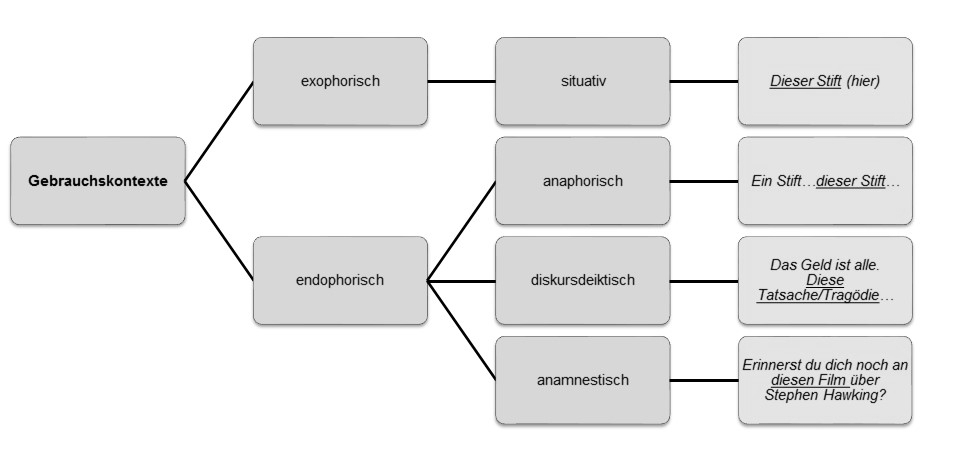
\includegraphics[width=12cm]{images/Gebrauchskontexte-demonstrativa-neu-sw.jpg}
\begin{forest}
for tree = {forked edges,grow'=east,anchor=east,minimum width=2cm,align=center,draw,s sep=\baselineskip}
[Gebrauchskontexte,rotate=90,anchor=north
  [exophorisch [ situativ,tier=isch [ \textit{Dieser Stift} (hier) ] ] ]
  [endophorisch
    [anaphorisch,tier=isch [ Ein Stift\ldots\textit{dieser Stift}\ldots ] ]
    [diskursdeiktisch,tier=isch [Das Zahlen steigen.\\\textit{Diese Entwicklung} ist\ldots ] ]
    [anamnestisch,tier=isch [ Erinnerst du dich noch\\an \textit{diesen Film} über\\Stephen Hawking? ] ]
  ]
]
\end{forest}
\caption {Gebrauchskontexte von Demonstrativa\label{abb:demonstrativa-gebrauchskontexte}}
\end{figure}



\subsection{Situativer Gebrauch}\label{sec:situativ}

Beim situativen \is{situativ} Gebrauch \parencite[auch deiktischer Gebrauch, z.B. bei][]{Bisle-Muller1991,Consten2004,Studler2011} führt der \isi{Demonstrativartikel} einen Referenten in das gemeinsame Diskursuniversum von Sprecher und Hörer ein, indem mit seiner Hilfe auf eine Entität in der unmittelbaren Äußerungssituation verwiesen wird, s. \REF{ex:deikt}.\footnote{In diesem und den folgenden Beispielen werden die relevanten Ausdrücke durch Kursivsetzung durch die Verfasserin hervorgehoben.}  Zugleich erfolgt eine Verortung im Raum.

\begin{exe}
	\ex \label{ex:deikt} \object{Dieser Stift} (hier) schreibt gut.
\end{exe}

Proximale Demonstrativa \is{Demonstrativum} kennzeichnen Entitäten, die dem Sprecher nahe\linebreak sind (z.B. \object{dieser}), distale markieren Distanz (z.B. \object{jener, dieser/der da}).
%\footnote{Diese Zweigliedrigkeit ist in allen Sprachen der Welt gegeben; zu komplexeren Systemen s. \textcite[35--55]{Diessel1999}.} 
Damit das Referieren glückt, müssen die Diskursteilnehmer ihr Wissen mit der Perspektive des Sprechers, dem deiktischen Zentrum oder  \object{origo} \parencite{Buhler1934} abgleichen  \parencite[s. auch][327--330]{Hoffmann2009}. Der Verweis kann mit einer Zeigegeste unterstützt werden; zu Ausnahmen und weniger zentralen Fällen des situativen \is{situativ} Gebrauchs s. \textcite[94--95]{Diessel1999} und \textcite[219--224]{Himmelmann1996}. 

Mit \textcite[]{Buhler1934} kann man den situativen \is{situativ} Gebrauch in zwei Arten des Zeigens unterteilen. Bei der sog. \object{Demonstratio ad oculos} zielt die Zeigegeste auf einen Referenten, der in der unmittelbaren Umgebung vorhanden und somit für die Diskursteilnehmer sichtbar ist (typisch für \object{Face-to-Face}-Kommunikation). Die sog. \object{Deixis am Phantasma} umfasst hingegen demonstrative Ausdrücke, die innerhalb der bloßen Vorstellung operieren: Der Referent wird zwar im Diskursuniversum verortet, ist aber nicht physisch anwesend \parencite[s. auch][222]{Himmelmann1996}. Dieser Gebrauch gilt für alle Kommunikationsformen, in denen Äußerungen zeitlich und räumlich vom Sprecher entkoppelt sind, also z.B. in narrativen Texten \parencite[95]{Diessel1999} oder auch in wissenschaftlichen Beschreibungen, in denen das deiktische Zentrum von einem imaginären Sprecher ausgeht. Der situative \is{situativ} Gebrauch ist in diesem Sinne auch in Dokumenten aus älteren Sprachstufen zu erwarten. 

Mit der situativen \is{situativ} Verortung -- sei sie konkret oder imaginär -- geht immer ein kognitiver Abgrenzungsprozess zu anderen potentiellen Referenten einher, etwa  \object{Ich möchte diesen (und nicht jenen) Stift} \parencite[vgl.][70]{Bisle-Muller1991}, wodurch der Referent eindeutig determiniert und identifiziert werden kann \parencite{Hoffmann2009}. 

 
\subsection{Anaphorischer Gebrauch}\label{sec:anaphorisch}

Während die eindeutige Determination beim situativen \is{situativ} Gebrauch über den außersprachlichen Kontext gewährleistet wird, kommt beim anaphorischen \is{anaphorisch} Ge"-brauch die textuelle Umgebung ins Spiel\footnote{Die textuelle Umgebung schließt sowohl schriftliche als auch mündlich Diskurstypen ein.}: Es wird auf einen zuvor im Diskurs etablierten Referenten verwiesen (den Antezedens), s. \REF{ex:anaph} basierend auf \textcite[][229]{Himmelmann1996}.{\interfootnotelinepenalty=10000\footnote{In Opposition hierzu stehen \object{kataphorische} Ausdrücke: Sie sind koreferentiell \is{Referentialität} mit nachfolgenden Referenten, welche erst im weiteren Diskursverlauf  hinreichend identifiziert werden können \parencite[s.][161--162]{Veldre-Gerner2007}. Beim vergleichsweise seltenen kataphorisch gebrauchten \isi{Demonstrativartikel} kann eine pejorative Lesart mitschwingen (\object{Auf der Party war dieser Student.}). Zur Diskussion solcher Verwendungsweisen als möglichen Ausdruck von \isi{Spezifizität} s. \textcite[533]{deMulder2011}.}}

\begin{exe}
	\ex \label{ex:anaph} Es war einmal ein König. \object{Dieser König} hatte drei Söhne...
\end{exe}

Im Vergleich zu anderen Mitteln der Wiederaufnahme \is{Personalpronomen}  (etwa Personalpronomen\linebreak oder \isi{Definitartikel}) zeichnen sich anaphorische \is{anaphorisch} \isi{Demonstrativartikel} (und Demonstrativa \is{Demonstrativum} allgemein) dadurch aus, dass sie eine (Neu-)Fokussierung von Referenten im Diskurs bewirken \parencite [s. u.a.][]{Ehlich1979,Prince1981,Gundel1993,Comrie1997,Himmelmann1996,Diessel1999,Kibrik2011}. Sie werden daher häufig gebraucht, um einen Topikwechsel \is{Topik} \isi{Informationsstruktur} zu vollziehen. In Beispiel \REF{ex:topic} \parencite[angelehnt an][96]{Diessel1999} impliziert das \isi{Personalpronomen} \object{er} Koreferentialität \is{Referentialität} mit dem \isi{Topik} \object{Anwalt}, während sich das \isi{Demonstrativum} \object{der} nur auf \object{Klient} beziehen kann, der zu diesem Zeitpunkt zwar kognitiv aktiviert, aber nicht fokussiert und \blockcquote[96]{Diessel1999}{somewhat unexpected} ist \parencite[vgl. hierzu][278--279]{Gundel1993}. Im Gegensatz hierzu ist die Wiederaufnahme des bereits im Fokus stehenden \object{Anwalt} mit \object{dieser Anwalt} blockiert. Am natürlichsten erscheinen die pronominalen \isi{Informationsstruktur} Wiederaufnahmen. Mit der \isi{Phrase} \object{dieser Klient} kann allerdings besonders stark betont werden, dass jetzt der Klient und nicht -- wie erwartet -- der Anwalt im Mittelpunkt des weiteren Diskursverlaufs steht.   

\begin{exe}
	\ex \label{ex:topic} Der Anwalt sprach mit einem Klienten. Da \object{er/der/dieser Klient/*dieser Anwalt} nur wenig Zeit hatte, vereinbarten sie ein weiteres Gespräch für die nächste Woche. 
\end{exe}

Das Potential, einen Topikwechsel \is{Topik} einzuleiten, lässt sich darauf zurückführen, dass es zur Hauptfunktion von Demonstrativa \is{Demonstrativum} gehört, Referenten, die gerade neu eingeführt wurden, anaphorisch \is{anaphorisch} wiederaufzunehmen.\footnote{Vgl. hierzu auch die Studie von \citeauthor{Fraurud1990}, in der empirisch belegt wird, dass schwedische \isi{Demonstrativartikel} fast ausschließlich anaphorisch \is{anaphorisch} gebraucht werden \parencite[400]{Fraurud1990}.} Dies gilt insbesondere für artikellose Sprachen  \parencite[229]{Himmelmann1996}, aber auch für Sprachen, die einen \isi{Definitartikel} ausgebildet haben, etwa das Englische. \citeauthor{Christophersen1939} beobachtet \blockcquote[vgl.][29]{Christophersen1939} {a certain aversion to the use of a \object{the}-form immediately after the word is introduced; a demonstrative is more usual in such cases}. Demonstrativa \is{Demonstrativum} sind also die erste Wahl, um ein \isi{Topik} im Diskurs nach Ersterwähnung des Referenten zu etablieren. Für die  anschließende referentielle Kontinuität \is{Informationsstruktur} sorgen \isi{Personalpronomen} oder \isi{Definitartikel}, indem sie das \isi{Topik} im Fokus der Aufmerksamkeit halten. 

\subsection{Diskursdeiktischer Gebrauch}\label{diskurs-deikt}

Werden \isi{Demonstrativartikel} zum Zwecke der Diskursdeixis \is{diskursdeiktisch} eingesetzt, verweisen sie nicht auf einzelne \is{Nominalphrase (NP)} NPs, sondern auf größere syntaktische Einheiten, also Sätze, Abschnitte oder Texte \parencite{Webber1991,Fraurud1992, Fillmore1997, Diessel1999, Consten2007, Consten2009, Marx2011}. Durch die anaphorische \is{anaphorisch} Wiederaufnahme werden die zuvor genannten Informationen zu einem abstrakten Referenten gebündelt (z.B. \object{Tatsache, Prozess, Zustand}) und können dann evaluierende Zusatzinformationen transportieren (\object{Ungerechtigkeit, Tragödie, Zufall}),  s. (\ref{diskurs}).\footnote{Da dieser anaphorische \is{anaphorisch} Prozess die \blockcquote[129]{Schwarz2000}{kognitive Strategie der Komplexbildung} voraussetzt, hat sich in neueren Arbeiten zur Textlinguistik der Begriff \object{Komplex-Anaphern} etabliert \parencite[s. z.b.][]{Consten2007, Consten2009}. Einen Überblick über weitere terminologische Vorschläge der letzten Jahrzehnte bietet \textcite[16--17]{Marx2011}, zur Abgrenzung von Diskursdeixis \is{diskursdeiktisch} und Anapher \is{anaphorisch} s. \textcite[30--31]{Consten2004}.} 

 \begin{exe}
	\ex \label{diskurs}  Jedes Jahr sind tausende Menschen auf der Flucht.
	\begin{xlist}
		\ex \label{propo} \object{Diese Tatsache} lässt viele erschauern.
			\ex \label{bewertung} \object{Diese Ungerechtigkeit} muss behoben werden.
		\end{xlist}
\end{exe}

Zwar kann der diskursdeiktische Gebrauch nur über einen anaphorischen \is{anaphorisch} Bezug gelingen, der eigentliche Referent wird allerdings erst zum Zeitpunkt des Verweises im Diskurs etabliert, wodurch die Diskursdeixis dem situativen \is{situativ} Gebrauchskontext ähnelt \parencite[224]{Himmelmann1996}. Beide Kontexte fallen typischerweise in die Domäne von pro- oder adnominalen Demonstrativa; ein Austausch mit dem \isi{Definitartikel} ist theoretisch möglich, aber markiert, vgl. (\ref{def-diskurs}); Beispiele nach  \textcite[130--131]{Schwarz2000}.  

 \begin{exe}
	\ex \label{def-diskurs} 
	\begin{xlist}
		\ex \label{ex:tassen} Er zerbrach bei der Feier eine sehr teure Vase. \object{Dieses/Das Missgeschick} blieb noch lange in Erinnerung. 
			\ex \label{ex:entwicklung} Die Arbeitslosigkeit steigt, die Inflation schreitet fort, die Wirtschaft ist rückläufig. \textit{Diese/}??\textit{Die Entwicklung} ist gefährlich. 
		\end{xlist}
\end{exe}

Die Faktoren, die bestimmen, dass NPs \is{Nominalphrase (NP)} mit \isi{Definitartikel} für den diskursdeiktischen \is{diskursdeiktisch} Gebrauch gewählt werden, sind bislang kaum erforscht. Mit der Korpusuntersuchung \is{Korpuslinguistik} von \textcite{Consten2007} ist allerdings empirisch belegt, dass \isi{Demonstrativartikel} das häufigste und damit unmarkierte Mittel sind, um im Deutschen diskursdeiktische \is{diskursdeiktisch} Bezüge herzustellen.

\subsection{Anamnestischer Gebrauch}\label{sec:amnamnestisch}

Beispiel \REF{ex:anamn} illustriert den anamnestischen \is{anamnestisch} Gebrauchskontext. Der Referent von  \object{dieser Aufsatz} wird als neue Information \is{Informationsstruktur} in den Diskurs eingeführt. Für die eindeutige Identifizierung muss der Rezipient allerdings vorhandenes Wissen aktivieren, d.h. Informationen, die im Langzeitgedächtnis gespeichert sind.

\begin{exe}
	\ex \label{ex:anamn} Hast du schon \object{diesen Aufsatz} von der neuen Kollegin gelesen?  
\end{exe}

Der Begriff \object{anamnestisch} \is{anamnestisch} geht auf \textcite{Buhler1934} zurück (von griech. \object{anámnesis} \extrans{Erinnerung}) und wurde von \textcite{Himmelmann1997} als deutsche Übersetzung des \object{recognitional use} \parencite{Himmelmann1996,Diessel1999}  eingeführt.

Die Voraussetzung für diesen Gebrauchskontext ist, dass die Diskursteilnehmer gleiche Erfahrungen über den gemeinten Referenten besitzen, etwa durch ein früheres Gespräch. \textcite[44]{Bisle-Muller1991} spricht in diesem Sinne von \object{konspirativem Wissen}; auch engl. \object{private information} \parencite[106]{Diessel1999}. Die Identifizierbarkeit des Referenten ist daher an die notwendige Mitwisserschaft des Hörers gekoppelt \parencite[72]{Szczepaniak2011a}. Für den Sprecher sind anamnestische \is{anamnestisch} Verweise besonders ökonomisch, da der Appell zur gemeinsamen Wissensaktivierung mit vergleichsweise geringen verbalen Kosten verbunden ist. Für den Hörer ist der (kognitive) Erinnerungsaufwand umso größer.

Nach \textcite[79--80]{Bisle-Muller1991} kann die Verwendung des Demonstrativartikels \is{Demonstrativartikel} in diesen Kontexten sogar als kommunikative Strategie genutzt werden, um eine mögliche Uneindeutigkeit des Referenten zu kennzeichnen, s. \REF{ex:auer} (Gesprächsbeispiel vereinfacht nach \citealt[637]{Auer1984}, vgl. auch \citealt[58]{Himmelmann1997}). Der Sprech"-er räumt sozusagen die Möglichkeit ein, dass es dem Hörer Schwierigkeiten bereiten könnte, einen eindeutigen Referenten für die Phrase \is{Phrase} \object{diesem Haustelefon} auszumachen. 

\begin{exe}
	\ex \label{ex:auer} 
	\begin{itemize}
		\item[A:] Was ist denn eigentlich mit \textit{diesem Haustelefon}, das ihr immer genutzt habt? 
		\item[B:] Das funktioniert nicht mehr. 
	\end{itemize}
\end{exe}

Die mögliche Referenzproblematisierung durch \object{dieser} schwingt beim \isi{Definitartikel} nicht mit, vgl. Beispiel \REF{ex:kinder} \parencites()()[][80]{Bisle-Muller1991}[][70]{Himmelmann1997}. Wenn von \object{den Kindern} gesprochen wird, ist die naheliegendste Interpretation, dass die eigenen Kinder gemeint sind; mit \object{diese Kinder} wird ein breiterer (und unerwarteter) Wissensrahmen eröffnet, der nur mit Bezug auf geteiltes Wissen eine eindeutige Referenz zulässt.    

\begin{exe}
	\ex \label{ex:kinder} Ich bringe heute \textit{die Kinder/diese Kinder} mit.   
\end{exe}

Der anamnestische \is{anamnestisch} wird neben dem anaphorischen \is{anaphorisch} Gebrauch als möglicher Übergangsbereich von Demonstrativ- zu \isi{Definitartikel} betrachtet (s. ausführlich die Diskussion in Abschnitt \ref{sec:bruecke}). Laut \textcite[73]{Himmelmann1997} sind für den anamne"-stischen Gebrauch \object{aktivierende Modifikatoren} typisch. Hierzu zählen bspw. das PP-Attribut \object{von der neuen Kollegin} aus Beispiel \REF{ex:anamn} oder restriktive Relativsätze wie in dem nachfolgenden Beispiel.

\begin{exe}
	\ex \label{ex:film} Sie geht in \textit{diese neue Schule, auf der man nicht sitzenbleiben kann}.    
\end{exe}
\noindent 
Die Beschreibung im Relativsatz soll dem Hörer oder der Hörerin helfen, sich den Referenten in Erinnerung zu rufen. Es wird vorausgesetzt, dass dem Adressaten die Schule (z.B. durch vorherige Gespräche) bekannt ist. Im Unterschied zu den \object{etablierenden Modifikatoren} (s. Abschnitt \ref{sec:nicht-fam}) nimmt die Identifikationshilfe im Relativsatz Bezug auf Wissen, das nur von den Diskursteilnehmern geteilt wird. Durch etablierende Modifikatoren wird ein Referent hingegen durch Einbezug von generellerem Wissen definiert und damit eindeutig identifiziert, etwa \object{Sie freut sich auf das Buch von George R.R. Martin, das morgen erscheint}. Weil die Grenze zwischen diesen beiden Modifikationsarten fließend sind, sind Brückenkontexte \is{Brückenkontext} hier wahrscheinlich \parencite[s. zur ausführlichen Diskussion][79--80]{Himmelmann1997}. 

\section{Gebrauchskontexte für Definitartikel}\label{sec:definitartikel}

Wie nachfolgend gezeigt wird, kann der \isi{Definitartikel} prinzipiell auch in den für das \isi{Demonstrativum} typischen Verwendungsweisen vorkommen, die in den vorhergehenden Abschnitten erläutert wurden (Abschnitt \ref{sec:definitartikel-in-demonstrativ}). Darüber hinaus gibt es Gebrauchskontexte, die alleine den Definitartikeln vorbehalten sind. Hierzu zählen der abstrakt-situative Gebrauch \is{abstrakt-situativ} (Abschnitt \ref{sec:abst-sit}), der assoziativ-anaphorische \is{assoziativ-anaphorisch} Gebrauch (\ref{sec:asso}), die sog. nicht-familiären (\ref{sec:nicht-fam}) und die nicht-referentiellen \is{Referentialität} Gebrauchs"-kontexte (Abschnitt\ref{sec:nicht-referentiell}). 

\subsection{Verwendung in demonstrativen Gebrauchskontexten}\label{sec:definitartikel-in-demonstrativ}

Belege für den situativen \is{situativ} und anaphorischen \is{anaphorisch} Gebrauch finden sich bei \textcite[110--111]{Hawkins1978} und \textcite[36]{Himmelmann1997}, s. \REF{ex:sitdef} und \REF{ex:anadef}; nachfolgend übersetzt und leicht gekürzt.\footnote{In der Forschung wird für die Kontextanalysen meist das Englische als Bezugssprache genommen \parencite{Christophersen1939, Lobner1985,Lyons1999}. Typologische Vergleiche finden sich in \textcite{Himmelmann1997}, für das Deutsche sei auf \textcite{Bisle-Muller1991} verwiesen.} Die Bedeutungsunterschiede sind in diesen Beispielen minimal: Beim \isi{Demonstrativum} schwingt aufgrund seiner deiktischen Kraft ein Abgrenzungsmoment zu anderen (wenn auch nicht explizit genannten) Referenten mit \parencite{Bisle-Muller1991}; außerdem hebt es den Topikwechsel \is{Topik} hervor.\footnote{Mit Akzentuierung (\object{dér}) kann auch der \isi{Definitartikel} in dieser Form verwendet werden.}   

\begin{exe}
	\ex \label{ex:sitdef} Reich mir bitte mal \textit{diesen/den Eimer}.  \\(situativer \is{situativ} Gebrauch)
	\ex \label{ex:anadef} Ein Mann erscheint mit einem Paket. Und \textit{dieses/das Paket}... \\(anaphorischer Gebrauch)
\end{exe}

Anders sieht es beim diskursdeiktischen \is{diskursdeiktisch} Gebrauch aus. Hier ist die Substitution mit einem \isi{Definitartikel} ebenfalls möglich, aber deutlich markiert, s. \REF{ex:diskurs-deikt-def}; Beispiel aus \textcite[95]{Marx2011}, vgl. auch Abschnitt \ref{diskurs-deikt}). Während die Phrase \is{Phrase} \object{diese Nachlässigkeit} den Zustand, den man aus dem vorher genannten Ereignis ableiten kann, klassifiziert und damit indirekt anaphorisch  \is{anaphorisch} ist, kann \object{die Nachlässigkeit} als allgemeine Last interpretiert werden, die \object{Robert} auszeichnet, im Sinne von \object{seine Nachlässigkeit}.

\begin{exe}
	\ex \label{ex:diskurs-deikt-def}  Anstatt für seine Prüfungen zu lernen, ist Robert im Kino gewesen. \textit{Diese\slash}?\textit{Die Nachlässigkeit} könnte ihn das Vordiplom kosten. \\(diskursdeiktischer Gebrauch)
	 \end{exe}

Auch beim anamnestischen \is{anamnestisch} Gebrauch kommt es zu Bedeutungsunterschieden, s. \REF{ex:anamndef}. Mit dem \isi{Definitartikel} unterstellt der Sprecher,  dass der Referent mit Rückbezug auf geteiltes Wissen problemlos identifiziert werden kann; die Phrase \is{Phrase} mit \isi{Demonstrativartikel} signalisiert hingegen, dass es möglicherweise nicht direkt klar ist, welcher Wissensrahmen aktiviert werden muss, um den Referenten zu verorten \parencite[79--80]{Bisle-Muller1991}. 
 
\begin{exe}
	\ex \label{ex:anamndef} Ich habe doch noch \textit{dieses/das Buch} gekauft. \\ (anamnestischer Gebrauch)
\end{exe}
 
Während in den nhd. Beispielen jeweils zwei Formen kontrastiert wurden (De"-mon"-strativ"-artikel \is{Demonstrativartikel} \object{dieser} vs. \isi{Definitartikel} \object{der}), gibt es im Althochdeutschen \object{eine} Form, die sowohl De"-mon"-strativ-"" \is{Demonstrativartikel} als auch \isi{Definitartikel} sein könnte, nämlich das ahd. \object{dër}. 
Wenn ein \object{dër}  in den bisher genannten Verwendungsweisen, den sog. pragmatischen \is{Pragmatische Definita} Definitheitskontexten (s. Abschnitt \ref{sec:pragsem}) genutzt wird, so kann man es folglich immer als Demonstrativartikel, aber nicht automatisch als \isi{Definitartikel} einordnen. Allgemeiner formuliert: Kommt ein Artikelwort in pragmatischen Definitheitskontexten \is{Pragmatische Definita} vor, ist dies keine  hinreichende Bedingung dafür, dass es sich um einen Definitartikel-, wohl aber um einen \isi{Demonstrativartikel} handelt. Wenn ein Artikelwort aber in den sog. semantischen Definitheitskontexten \is{Semantische Definita} auftritt, betritt es die Domäne des Definitartikels. Zu diesen zählen die abstrakt-situativen \is{abstrakt-situativ} und die assoziativ-anaphorischen \is{assoziativ-anaphorisch} Gebrauchskontexte, die in den folgenden Abschnitten besprochen werden. 



\subsection{Abstrakt-situativer Gebrauch}\label{sec:abst-sit}

Abstrakt-situative \is{abstrakt-situativ} Gebrauchskontexte zeichnen sich dadurch aus, dass ein Referent auch unabhängig von der Gesprächssituation eindeutig bestimmt werden kann \parencite[daher auch \object{larger situation use}, vgl.][115]{Hawkins1978}. Der  Referent ist also nicht in deiktischer inner- oder außersprachlicher Reichweite, sondern wird über das Weltwissen erschlossen. Dabei kann der jeweilige Wissensrahmen, in dem der Referent verortet wird, variieren. Die definiten NPs \is{Nominalphrase (NP)} in \REF{ex:abstrakt-situativ} basieren bspw. auf der Erfahrung, dass eine Stadt typischerweise \object{ein} Rathaus (\ref{ex:rathaus}),  Deutschland \object{eine}  Bundeskanzlerin (\ref{ex:merkel})  und unsere Erde \object{einen} Mond (\ref{ex:mond}) hat. Die Beispiele setzen also voraus, dass die Referenten \is{abstrakt-situativ} in einem bestimmten Bezugsrahmen \object{einzigartig} \parencite{Russell2006} sind. 

 \begin{exe}
	\ex \label{ex:abstrakt-situativ}   
	\begin{xlist}
		\ex \label{ex:rathaus} Wir treffen uns vor \textit{dem Rathaus}.
		\ex \label{ex:merkel} \textit{Die Bundeskanzlerin} kommt zu Besuch.
		\ex \label{ex:mond} Gestern schien \textit{der Mond} besonders hell.
		\end{xlist}
\end{exe}

Wichtig ist, dass die Diskursteilnehmer denselben Bezugsrahmen aktivieren. Beispielsweise gibt es theoretisch unendlich viele Personen, auf die mit \object{der Bräutigam} in \REF{ex:braut} referiert werden kann, aber innerhalb eines spezifischen situativen Rahmens (hier das Gespräch über eine bestimmte Hochzeit, auf der es dem Weltwissen nach zu urteilen typischerweise einen Bräutigam gibt), können die Diskursteilnehmer präsupponieren, dass die Referenz eindeutig ist \parencite[Beispiel in Adaption an][41]{Studler2011}. Ebenso ist für Diskursteilnehmer \object{die Kneipe} in \REF{ex:kneipe} eindeutig identifizierbar, wenn es um die Kneipe geht, in der man sich regelmäßig trifft \parencite[36]{Himmelmann1997}.

\begin{exe}
	\ex \label{ex:abstrakt-situativ2}   
	\begin{xlist}
		\ex \label{ex:braut} Kanntest du \textit{den Bräutigam} gut?
		\ex \label{ex:kneipe} Wir treffen uns in \textit{der Kneipe}.  
		\end{xlist}
\end{exe}

Ein \isi{Unikum} wie \object{der Mond} ist hingegen weitaus weniger kontextsensitiv; seine Identifizierbarkeit ist fast in jedem Gespräch und zu jeder Zeit gesichert \parencite[549]{Schroeder2006}. \textcite[40--41]{Studler2011} folgend lässt sich die abstrakt-situative \is{abstrakt-situativ} Verwendungsweise von Definitartikeln \is{Definitartikel} daher aufteilen in \object{absolut-uniken} (bei\linebreak Unika) \is{Unikum} und \object{situativ-uniken} Gebrauch (wie in \ref{ex:braut}). In beiden Kontexten ist der Austausch mit einem \isi{Demonstrativartikel} nicht möglich. 

Nach \citeauthor{Schroeder2006} zählt auch der Verweis auf Institutionen wie in \REF{ex:post} zum abstrakt-situativen \is{abstrakt-situativ} Gebrauchskontext \parencite[vgl. auch][110]{Nubling2005}:  \blockcquote[549]{Schroeder2006}{As an institution, \object{the post office} may refer uniquely, even if I and the person I am speaking to merely share the context of living in a country with an institutionalized postal service}. 

\begin{exe}
	\ex \label{ex:post} Ich gehe \textit{zur Post}.
\end{exe}

\noindent
Die Beispiele in \REF{ex:rathaus} und \REF{ex:kneipe} können ebenfalls eine solche Institutionslesart haben. Weil kein spezifischer Referent denotiert wird, ergibt sich in diesen Fällen eine konzeptuelle Nähe zu nicht-spezifischen \is{Spezifizität}
 Gebrauchskontexten, s. Abschnitt \ref{sec:nicht-referentiell}.

Abstrakt-situative \is{abstrakt-situativ} Verwendungen weisen zudem Überschneidungspunkte mit dem anamnestischen \is{anamnestisch} Gebrauch auf \parencite[62]{Himmelmann1997}. In beiden Fällen wird erst über die Aktivierung von gemeinsamem Wissen ein Rahmen geschaffen, der die Identifizierbarkeit eines Referenten ermöglicht. Der Unterschied liegt darin, dass es sich bei der anamnestischen \is{anamnestisch} Verwendung um für die Diskursteilnehmer exklusives und auf spezifische Erfahrungen basiertes Wissen handelt, während der abstrakt-situative \is{abstrakt-situativ} Gebrauch auf Erfahrungen basiert, die ins Allgemeinwissen übergegangen sind. 

\subsection{Assoziativ-anaphorischer Gebrauch}\label{sec:asso}

Der assoziativ-anaphorische \is{assoziativ-anaphorisch} Artikelgebrauch liegt vor, wenn sich die definite Referenz aus einem Assoziationsverhältnis ergibt, das durch einen vorhergehenden Ausdruck im Text -- dem \object{trigger} \parencite[49]{Hawkins1978} oder \object{Anker} \parencite[6]{Cui2014} -- ausgelöst wird. So ist der \object{Kellner} in \REF{ex:asso} über eine Assoziationskette mental aktiviert, wenn über einen Restaurantbesuch gesprochen wird \parencite[Beispiel in Anlehnung an][50]{Schwarz2000}. Neben dem Terminus \is{assoziativ-anaphorisch} \object{assoziativ-anaphorisch}, der auf die Definitartikel-Typologie von \textcite{Hawkins1978} zurückgeht, werden in der Forschung u.a. die Begriffe  \object{bridging} \parencite{Clark1977}, \object{inferables} \parencite{Prince1981} oder \object{indirekte Anaphorik} \parencite{Schwarz2000} für diesen Gebrauchskontext verwendet.  

\begin{exe}
	\ex \label{ex:asso} Wir besuchten gestern ein Restaurant. [Anker] \\ 
	\textit{Der Kellner} [= assoziativ-anaphorische \is{assoziativ-anaphorisch} NP] war sehr nett zu uns. \end{exe}
\noindent 
Wichtig ist, dass das Bezugselement und der daran anknüpfende definite Ausdruck in einer \blockcquote[36]{Himmelmann1997}{kulturell oder sachlich vermittelten} Assoziationsrelation stehen, ansonsten ist die Textkohärenz gestört, s. \REF{ex:hund} im Vergleich zu \REF{ex:auspuff}; die Bespiele basieren auf \textcite[123]{Hawkins1978}.

 \begin{exe}
	\ex \label{ex:asso2}   
	\begin{xlist}
		\ex \label{ex:auspuff} Ein Auto fuhr an uns vorbei. \textit{Der Auspuff} stank. 
		\ex \label{ex:hund} Ein Auto fuhr an uns vorbei. \textit{Der Hund} bellte.
		\end{xlist}
\end{exe}

Mentale Assoziationsketten können also auf Teil-Ganzes-Re"-la"-tio"-nen beruhen (ein Auspuff ist ein typischer Bestandteil von Autos, ein Hund nicht), s. auch \REF{ex:meronymie}. Weitere Typen der \object{Verankerung} erörtert \textcite[98--122]{Schwarz2000}: Der semantische Valenzrahmen von Verben eröffnet bspw. Leerstellen für Partizipantenrollen, \is{Semantische Rolle} die als Bezugspunkt für assoziative Anaphern dienen können, s. \REF{ex:rolle}. Ein nominaler Ausdruck wie \object{das Krankenhaus} aktiviert ein kognitives \isi{Schema} mit bestimmten Standardwerten (etwa \object{Ärzte, Personal, Zimmer}), auf die indirekt verwiesen werden kann, s. \REF{ex:krank}. 

\begin{exe}
	\ex \label{ex:asso3}   
	\begin{xlist}
		\ex \label{ex:meronymie} Dort steht ein \is{Metonymie} Haus. \\ \textit{Das Fenster/die Tür/der Balkon} ist blau gestrichen. (Teil-Gan"-zes-Re"-la"-tion)
		\ex \label{ex:rolle} Heute wurde über eine Entführung berichtet. \\ \textit{Die Kidnapper} (=\,Agensrolle \isi{Agentivität} von \object{entführen}) fordern ein hohes Lösegeld.
				\ex \label{ex:krank} Sie musste ins Krankenhaus. \\ \textit{Die Ärzte/die Pfleger/das Wartezimmer}...\\(Standard-Werte für das Krankenhaus-Schema)
		\end{xlist}
\end{exe}

Ähnlich wie beim abstrakt-situativen \is{abstrakt-situativ} Gebrauchskontext wird enzyklopädisches Wissen bzw. auf Erfahrungen basierendes Weltwissen \hervor{angezapft}, das unabhängig von der Äußerungssituation für die notwendige Identifizierbarkeit des Referenten sorgt. Der Austausch mit einem \isi{Demonstrativartikel} ist in diesen Fällen entweder nicht möglich oder mit einer Bedeutungsverschiebung verbunden, z.B. mit einem pejorativen Unterton \parencite[989]{Hauenschild1993}. Wenn ein adnominales Element regelmäßig in abstrakt-situativen \is{abstrakt-situativ} und assoziativ-anaphorischen \is{assoziativ-anaphorisch} Kontexten verwendet wird, ist daher eine Einordnung als \isi{Definitartikel} gerechtfertigt \parencite[190]{Himmelmann1997}.

\subsection{Nicht-familiärer Gebrauch}\label{sec:nicht-fam}

\textcite[130--149]{Hawkins1978} führt unter den sog. \object{unfamiliar usages} unterschiedliche Gebrauchs"-typen an, in denen der \isi{Definitartikel} im Englischen gesetzt wird. Sie wurden von ihm als Gegenbeispiele für \citeauthor{Christophersen1939}s \object{familiarity}-Theorie zusammengetragen und gelten deswegen als nicht-familiär. Bei den entsprechenden definiten Ausdrücken handelt es sich jeweils um komplexe \is{Nominalphrase (NP)} No"-minal"-phrasen, d.h. der Kopf wird mit bestimmten Attributen modifiziert. Die nachfolgenden Beispiele \parencite[vgl. die Übersicht in][37]{Himmelmann1997} wurden aus dem Englischen übersetzt.
 
\begin{itemize} 
 		\item[a)] \label{etab} NP \is{Nominalphrase (NP)} mit etablierendem Relativsatz: \\ Was ist mit Bill los? -- \textit{Die Frau}, mit der er ausgegangen ist, war gemein zu ihm. 
		\item[b)] \label{komp} NP \is{Nominalphrase (NP)} mit Komplementsatz: \\ Bill ist begeistert von \textit{der Tatsache}, dass es so viel Leben auf der Erde gibt. 
		\item[c)] \label{gen-attr} NP \is{Nominalphrase (NP)} mit \is{Genitivattribut} genitivischen Attributen: \\ \textit{der Anfang} des Krieges, \textit{die erste Seite} vom Guardian
		\item[d)] \label{n-attr} NP \is{Nominalphrase (NP)} mit nominalen Attributen: \\ \textit{das Alter} Sieben, \textit{die Farbe} Rot
\end{itemize}

Wie \textcite[38]{Himmelmann1997} anmerkt, unterscheidet sich die NP \is{Nominalphrase (NP)} mit etablierendem Relativsatz von allen anderen nicht-familiären Gebrauchsweisen dadurch, dass hier auch ein indefiniter Artikel \is{Indefinitartikel} verwendet werden kann (\object{eine Frau, mit der...}). Da auch ein \isi{Demonstrativartikel} im Sinne des anamnestischen \is{anamnestisch} Gebrauchs möglich wäre (\object{diese Frau, mit der...}), ist dieser Kontext also nicht exklusiv den Definitartikeln vorbehalten. Nach \textcite[308]{Lobner1985} kann man den Satz mit einem anaphorischen \is{anaphorisch} Verweis paraphrasieren, s. \REF{ex:bill}. %Entsprechend liegt in \REF{ex:bill} eine Katapher vor. 

\begin{exe}
	\ex \label{ex:bill} Was ist mit Bill los? -- Er ist gestern mit einer Frau ausgegangen und \textit{diese Frau/die Frau} war gemein zu ihm. 
\end{exe}

In den übrigen Fällen ist ein Austausch mit \isi{Demonstrativartikel} nicht möglich, denn hier sorgen die Attribute für die Eindeutigkeit des Referenten. Es liegen dann jeweils abstrakt-situative \is{abstrakt-situativ} Gebrauchskontexte vor, in denen die Köpfe der NPs \is{Nominalphrase (NP)} wie Unika \is{Unikum} interpretiert werden  \parencite[38]{Himmelmann1997}. 

Als weitere \object{modifier}, die dazu führen, dass eine NP \is{Nominalphrase (NP)} von einem \isi{Definitartikel} begleitet werden muss, nennt  \textcite[148 und 228--230]{Hawkins1978} \object{same}, \object{only}, \object{next} und \object{first} sowie \is{Superlativ} Superlative, vgl. die Beispiele in \REF{ex:mod}; vgl. zur Diskussion \textcite[9]{Lyons1999}.

 \begin{exe}
	\ex \label{ex:mod}   
	\begin{xlist}
		\ex \label{ex:same} Ich habe \textit{die gleiche Jacke} wie du.
		\ex \label{ex:only} Sie waren \textit{die einzigen Besucher}.   
		\ex \label{ex:next} \textit{Der nächste Anrufer} gewinnt ein Auto. 
		\ex \label{ex:first} \textit{Der erste Kunde} musste lange anstehen.  
		\ex \label{ex:super} Es war \textit{das schönste Kompliment} seit Jahren.
		\end{xlist}
\end{exe}

Weder ein \isi{Indefinitartikel} noch ein \isi{Demonstrativartikel} kann in diesen Fällen als Phraseneinleiter \is{Phrase} verwendet werden, da jeweils nur ein einziger Referent bzw. eine bestimmte Referentengruppe in Frage kommt, auf den die jeweilige Beschreibung zutrifft.  

\subsection{Nicht-referentielle Gebrauchskontexte}\label{sec:nicht-referentiell}

Alle bislang diskutierten Gebrauchskontexte zählen zum referentiellen \is{Referentialität} Artikelgebrauch, d.h. der definite Ausdruck referiert auf eine für die Diskursteilnehmer identifizierbare Entität in der außersprachlichen Wirklichkeit.
Der \isi{Definitartikel} kann im Gegenwartsdeutschen allerdings auch in nicht-referentiellen \is{Referentialität} Gebrauchsweisen zum Einsatz kommen und zwar in generischen \is{generisch} Aussagen und bei NPs \is{Nominalphrase (NP)} mit nicht-spezifischen \is{Spezifizität}  Referenten.\footnote{Mit dieser Subkategorisierung wird hier ein relativ weites Konzept von Nicht-Referentialität \is{Referentialität} angesetzt \parencite[zur Abgrenzungsdiskussion von \isi{Definitheit}, \isi{Spezifizität} und \isi{Referentialität} vgl. u.a.][]{Bisle-Muller1991,Lyons1999,Studler2011,vonHeusinger2011}.} 

%\subsubsection{(a) Generischer Gebrauch}\label{sec-generisch}

Generische Aussagen \is{generisch} zeichnen sich dadurch aus, dass nicht ein bestimmtes Individuum fokussiert, sondern eine Aussage über eine Gattung gemacht wird, s. \REF{ex:gener}; übersetzt und gekürzt aus \textcite[]{Krifka1995}. Hierbei wird zwischen den sog. \object{kind-referring} NPs \is{Nominalphrase (NP)} ohne und mit \object{characterizing sentences} unterschieden.   

\begin{exe}
	\ex \label{ex:gener}   
	\begin{xlist}
		\ex \label{ex:sued} \textit{Die Kartoffel} stammt aus Südamerika. (\object{kind-referring} NP)
		\ex \label{ex:vitc} \textit{Die Kartoffel} enthält Vitamin C. (\object{kind referring} NP \is{Nominalphrase (NP)} mit \object{characterizing sentence})
		\end{xlist}
\end{exe}

In Beispiel \REF{ex:sued} wird mit \object{die Kartoffel} nicht auf ein bestimmtes Individuum referiert, sondern eine verallgemeinerte Aussage über die Gattung \object{Kartoffel} gemacht. \textcite[2]{Krifka1995} bezeichnen diesen NP-Typ daher als \object{kind-referring}; auch \object{intensionale Generalisierung} \parencite[138]{Bisle-Muller1991}. Die Aussage lässt sich nicht auf ein einzelnes Individuum beziehen, sondern ist das Resultat einer Abstraktion. Die generische \is{generisch} Lesart der NP \is{Nominalphrase (NP)} ist den sog. \object{kind predicates} geschuldet, wie \object{üblich sein, verbreitet sein, ausgestorben sein, stammen aus} \parencite{Krifka1995}. Ein Subtyp sind die sog. \object{kind-referring} NPs mit \object{characterizing sentences}, die (theoretisch) jedes Individuum einer Art beschreiben; auch \object{extensionale Generalisierung}  \parencite[139--140]{Bisle-Muller1991}. Die Verallgemeinerung wird durch einzelne Ausnahmen nicht ungültig: \blockcquote[179]{Lyons1999}{[G]enerics admit exceptions, since they express general tendencies}. So ist die Aussage  \object{die Katze hat vier Beine} immer noch haltbar, selbst wenn Katzen existieren, die nur drei Beine haben.

In beiden Fällen kann die NP \is{Nominalphrase (NP)} auch durch eine artikellose Pluralform \is{Numerus} ersetzt werden, s. \REF{ex:sued2}. 
Weitere Varianten generischer \is{generisch} NPs \is{Nominalphrase (NP)} sind im Gegenwartsdeutschen nur bei den \object{characterizing sentences} möglich, etwa der Austausch mit einer indefiniten \is{Indefinitheit} singularen NP \is{Nominalphrase (NP)} oder die Determination mit \object{jeder} oder \object{all} \parencite[296]{Duden2009}, vgl. \REF{ex:vitc2}. 

\begin{exe}
	\ex \label{ex:gener3}   
	\begin{xlist}
		\ex \label{ex:sued2} Kartoffeln stammen aus Südamerika und enthalten Vitamin C. 
		\ex \label{ex:vitc2}  Eine/Jede Kartoffel enthält Vitamin C.\\
		*Eine/*Jede Kartoffel stammt aus Südamerika.
		\end{xlist}
\end{exe}

Es ist anzumerken, dass es sprachübergreifend keine grammatische Form gibt, die ausschließlich dazu dient, Generizität \is{generisch} anzuzeigen; es existieren also keine genuinen Generizitätsmarker \parencite[190]{Gerstner-Link1995}. Eine NP \is{Nominalphrase (NP)} wie \object{die Kartoffel} erhält erst abhängig von der Prädikation und vom jeweiligen Kontext eine generische \is{generisch} Lesart. Disambiguierend können Adverbien \is{Adverb} wie \object{immer} oder \object{generell} sein. 

Generisch \is{generisch} kann nur ein \isi{Definitartikel} gebraucht werden, der seine ursprünglich demonstrativen und deiktischen Bedeutungskomponenten eingebüßt hat. Denn es gibt keinen bestimmten Referenten, den es in der außersprachlichen Welt zu identifizieren gilt, sondern nur eine Art, über die beschreibende Aussagen getroffen werden. Deswegen ist die NP \is{Nominalphrase (NP)} selbst nicht referierend, sondern nur beschreibend \parencite[297]{Bluhdorn2008}. Der generische \is{generisch} Gebrauch markiert also eine späte Stufe der Artikelentwicklung. Sprachübergreifend führt dies zu synchroner Variation: Während es im Französischen bspw. obligatorisch ist, plurale \object{kind referring} NPs \is{Nominalphrase (NP)} in \object{characterizing sentences} mit einen \isi{Definitartikel} auszustatten, sind im Deutschen Sätze dieser Art für viele Sprecherinnen und Sprecher nicht akzeptabel, vgl. \REF{ex:gener2}; basierend auf den Ausführungen von \textcite{Lyons1999} und \textcite{Barton2016}.

\begin{exe}
	\ex \label{ex:gener2} 
	\begin{xlist}
		\ex[]{\label{ex:frz}  \textit{Les chats} sont des mammifères.}
		\ex[?]{\label{ex:dt} \textit{Die Katzen} sind Säugetiere.}
		\end{xlist}
\end{exe}

\textcite{Himmelmann1997} ordnet generische \is{generisch} Aussagen zu den abstrakt-situativen \is{abstrakt-situativ} Gebrauchskontexten und begründet dies folgendermaßen: \blockcquote[37]{Himmelmann1997}{Es gehört zum Sprachwissen (das als Teil des Weltwissens anzusehen ist), daß mit einem Lexem auf eine Klasse, und zwar typischerweise auf genau eine Klasse, von Elementen referiert werden kann. Wer die Bedeutung eines Lexems versteht, kennt auch die Klasse (Art, Typus) der Elemente, die damit bezeichnet werden. Damit liegen dieselben Verwendungsbedingungen vor wie bei \object{the sun} oder \object{the pub} (generelles Wissen über die Beschaffenheit der Welt). Daß die Art des Referenten unterschiedlich ist (ein Individuum bzw. eine Klasse), ist hinsichtlich des Gebrauchs des Definitartikels unerheblich.}

Diese Sichtweise ist konform mit Hawkins' Idee der \object{inclusiveness}:  \blockcquote[43]{Studler2011}{Bereits Hawkins (1978) hat darauf aufmerksam gemacht, dass der generische \is{generisch} Gebrauch zum uniken Gebrauch gezählt werden muss. Er hat in seiner Inclusiveness-Theorie argumentiert, dass bei der generischen \is{generisch} Verwendung auf eine Totalität Bezug genommen wird. Diese Totalität entspricht einem inklusiven Set, d.h. die Gesamtheit
aller Elemente einer Klasse. Auf diese Weise wird auf einen einzigen Gegenstand (als
Menge) referiert. Die unike \is{Unikum} Bezugnahme auf ein Einzelding stellt dabei einen Sonderfall
dar, indem die Menge hier zufällig aus genau einem Element besteht.} 


%\subsubsection{(b) Nicht-spezifischer Gebrauch}\label{nicht-spez}

Auch in den nachfolgenden Fällen, in denen  auf keinen spezifischen Referenten \isi{Spezifizität} verwiesen wird, handelt es sich um nicht-referentielle \is{Referentialität} \is{Nominalphrase (NP)} NPs. 

\begin{exe}
	\ex \label{ex:nonref}   
	\begin{xlist}
		\ex \label{ex:schule-pia} Pia geht \textit{zur Schule}. 
		\ex \label{ex:fvg} Wir bringen das Stück \textit{zur Aufführung}.
		\end{xlist}
\end{exe}
\noindent 
In \REF{ex:schule-pia} gibt es keinen zu identifizierenden Referenten für \object{Schule}, sondern es wird ausgedrückt, dass Pia die Institution \object{Schule} besucht und damit schulpflichtig ist. Sprecher und Hörer haben also keinen bestimmten Referenten im Kopf, der in Zeit und Raum lokalisierbar wäre \parencite[40]{Bisle-Muller1991}. Beispiele wie diese werden im Gegensatz zum spezifischen \is{Spezifizität} Gebrauch (Pia geht zu \textit{der Schule}, die uns empfohlen wurden), wie \textcite[245]{Studler2011} anmerkt, auch als generisch \is{generisch} klassifiziert \parencite[ähnlich][90]{Szczepaniak2011a}. Um diese Fälle von den oben genannten generischen \is{generisch} Ausdrücken abzugrenzen, bietet es sich an, einen anderen Terminus zu wählen und daher \textcite[54]{Bisle-Muller1991} folgend von \object{nicht-spezifischem} Gebrauch zu sprechen.\footnote{Zur Diskussion der Kategorie \object{\isi{Spezifizität}} als kategoriale Stufe in der Entwicklung des Definitartikels s. Abschnitt \ref{sec:stufen}.} Auch \isi{Funktionsverbgefüge} wie in \REF{ex:fvg} enthalten NPs \is{Nominalphrase (NP)} ohne referierende Funktion. In Kombination mit dem desemantisierten \object{bringen} bildet \object{zur Aufführung} ein mehrgliedriges Prädikat, das eine Verbalhandlung denotiert, ohne auf eine partikuläre Aufführung zu verweisen. Entsprechend ist eine Attribuierung (?\object{zur schönen Aufführung}) nicht möglich.\footnote{Ähnliches lässt sich über Objektinkorporierungen \is{Objektinkorporierung} wie \object{Kuchen essen} oder \object{Auto fahren} sagen.} Weil Art und Form des Artikels in diesen Fällen immer fest sind, spricht der Duden von \object{gebundenem} Artikelgebrauch \parencite[297--298]{Duden2009}. Auch in festen Wendungen oder Sprichwörtern liegt dieser Gebrauchstyp vor, s. \REF{ex:sprichwort}.   

\begin{exe}
	\ex \label{ex:sprichwort}   
	\begin{xlist}
		\ex \label{ex:zeilen} zwischen \textit{den Zeilen} lesen, \textit{ans Licht} kommen 
		\ex \label{ex:fest} Man soll \textit{den Tag} nicht vor \textit{dem Abend} loben. 
		\end{xlist}
\end{exe}

Die hier vorgestellten Gebrauchskontexte sind höchst konventionalisiert und entsprechen einem relativ spätem Stadium der Artikelentwicklung, da sie den vollständigen Verlust der ursprünglich demonstrativen Bedeutungskomponente voraussetzen. Für die Anfangsphase der Artikelentwicklung, die in dieser Arbeit vordergründig untersucht wird, spielen sie daher eine untergeordnete Rolle.


\section{Pragmatische und semantische Definitheit}\label{sec:pragsem}

Als übergeordnete Klassifikation für die in den vorherigen Abschnitten diskutieren Gebrauchskontexte hat sich in der Forschung die Löbnersche Unterscheidung in pragmatische \is{Pragmatische Definita} und semantische Definita \is{Semantische Definita} \parencite{Lobner1985} etabliert \parencite{Himmelmann1997, Demske2001,Nubling2005,Napoli2009,Szczepaniak2011a}. Zu den pragmatischen Definita \is{Pragmatische Definita} zählen \is{Nominalphrase (NP)} Nominalphrasen, die nur unter Einbezug des unmittelbaren Kontextes eindeutig referieren. \isi{Semantische Definita} sichern auch situationsunabhängig eine eindeutige Referenz. Hinter der Einteilung steht die Idee, dass Nomen unterschiedlich interpretiert werden können und zwar je nachdem, ob sie als sortale, relationale oder funktionale Konzepte fungieren \parencite{Lobner1985,Lobner1998}. Die nachfolgende Übersicht gibt diese Klassifikation vereinfacht wieder. 

\begin{itemize} 
		\item[a)] \label{sort} Sortale Konzepte: \\ Klassifikation von Objekten gemäß bestimmter Eigenschaften, die den potentiellen Referenten auszeichnen, z.B.  \object{Frau, Hund}
		\item[b)] \label{relat} Relationale Konzepte: \\  Charakterisierung von Objekten gemäß der Beziehung, in der sie zu anderen Objekten stehen (1:n Relation), z.B. \object{Schwester}, \object{Freund} 
		\item[c)] \label{funkt} Funktionale Konzepte (Untergruppe der relationalen Konzepte): \\  Zwei Objekte stehen in einer eindeutigen (nicht ambigen) Beziehung zueinander (1:1 Relation), z.B: \object{Ehefrau, Kopf, Wetter} 
\end{itemize} 

\noindent
\isi{Semantische Definita} sind \is{Nominalphrase (NP)} NPs, die einem funktionalen Konzept entsprechen, das unabhängig von der jeweiligen Situation aktiviert wird, vgl. die Definition in \REF{semdef}. 

\begin{exe}
	\ex \label{semdef}  An NP is a semantic definite iff it represents a functional concept, independently of the particular situation referred to. \parencite[299]{Lobner1985}
\end{exe}

Eigennamen \is{Eigenname} gelten als typische Beispiele für semantische \is{Semantische Definita} Definita, da sie eindeutig und kontextunabhängig auf eine bestimmte Entität referieren (=\,1:1 Relation). Wie \textcite[299--307]{Lobner1985} zeigt, lassen sich aber auch \is{Gattungsname} Appellativa, die in abstrakt-situativen \is{abstrakt-situativ} oder assoziativ-anaphorischen \is{assoziativ-anaphorisch} Kontexten verwendet werden, als funktionale Konzepte und damit als semantische Definita \is{Semantische Definita} klassifizieren, \parencite[s. hierzu auch ausführlich][104--110]{Demske2001}. Sie verlangen eine Markierung durch den \isi{Definitartikel} oder müssen anderweitig determiniert werden (z.B. durch Possessiva).\footnote{Ausnahmen finden sich bspw. bei Existenzprädikationen, etwa: \object{Besitzen Einzeller ein/*das Gehirn?} \is{Prädikativ} in Anlehnung an \textcite[297]{Lobner1985} oder bei festen Wendungen, z.B. \object{to go to school, face to face} \parencite[311]{Lobner1985}.}
Der \isi{Demonstrativartikel} ist hingegen bei semantischen Definita \is{Semantische Definita} blockiert. Seine Domäne sind die pragmatischen \is{Pragmatische Definita} Definita, welche dadurch charakterisiert sind, dass ihr Kopf einem sortalen oder relationalen (aber nicht funktionalen) Konzept entspricht. Erst durch den Kontext, d.h. mit Rekurs auf die textuelle oder außersprachliche Umgebung, ist die Eindeutigkeit der Referenz gewährleistet \parencite[307]{Lobner1985}. 

Ein entscheidender Vorteil an \citeauthor{Lobner1985}s Theorie ist, dass sich auch nicht-re"-feren"-tiel"-le Gebrauchsweisen des Definitartikels erfassen lassen (vgl. Abschnitt \ref{sec:nicht-referentiell}). Es geht nämlich primär nicht darum, ob auf einen  identifizierbaren Referenten in der außersprachlichen Umgebung referiert wird, sondern, ob das funktionale Konzept eine eindeutige Verlinkung zu einer bestimmten Situation bewirkt \parencite[304--307]{Lobner1985}. 
\tabref{abb:definita} zeigt, wie sich die in Abschnitt \ref{sec:demonstrativartikel} und \ref{sec:definitartikel} diskutierten Gebrauchskontexte auf die beiden Definitheitstypen verteilen \parencite[angelehnt an und erweitert nach][73]{Szczepaniak2011a}. 

Die konzeptuelle Unterscheidung in semantische und pragmatische Definita \is{Pragmatische Definita} reflektieren auch  die Verschmelzungsprinzipien von Präposition und \isi{Definitartikel} im Gegenwartsdeutschen \parencite[311--312]{Lobner1985}. \textcite[109--110]{Nubling2005} zeigt, dass Klisen \is{Klitikon} wie \object{im, am, ins} nur bei semantisch-definiten NPs \is{Nominalphrase (NP)} \is{Semantische Definita} möglich sind. Sie fasst darunter sowohl referentielle \is{Referentialität} als auch nicht-referentielle Fälle, z.B. konkrete Zeitpunkte (\object{Wir treffen uns am Montag\slash am 4. April}),  Substantivierungen (\object{Vom Rauchen wird ihm schlecht}), generische \is{generisch} Ausdrücke (\object{Die Evolution vom Wolf zum Hund}) oder feste Wendungen (\object{zur Entfaltung kommen}). 

\begin{sidewaystable}
\small
% % 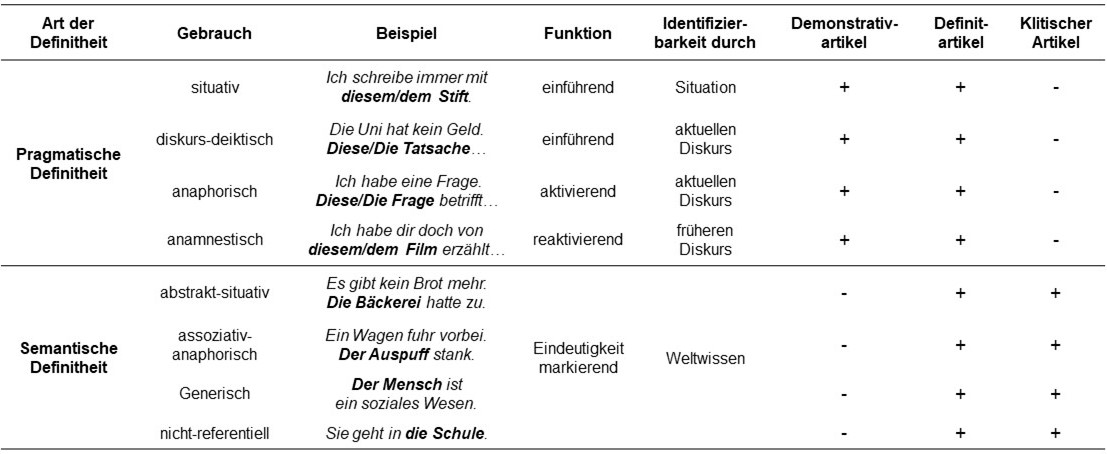
\includegraphics[width=\textwidth]{images/definit-kontexte-transparent.jpg}
\caption {Pragmatische und semantische Definita \is{Pragmatische Definita} \is{Semantische Definita} und ihre Gebrauchskontexte. (\textsc{dem}: Demonstrativartikel, \textsc{def}: Definitartikel, \textsc{klt}: Klitischer Artikel)\label{abb:definita}}
\begin{tabularx}{\textwidth}{>{\raggedright}p{\widthof{diskurs-deiktisch }}Q>{\centering}p{\widthof{reaktivierend}}cccc}
\lsptoprule
Gebrauch & Beispiel & Funktion & Identifizierbarkeit & \textsc{dem} & \textsc{def} & \textsc{klt}\\
         &          &          & durch \\\midrule                          
\multicolumn{7}{c}{Pragmatische Definitheit}\\\midrule
situativ & Ich schreibe immer mit \textit{diesem\slash dem Stift}. & einführend & Situation & + & + & \textminus\\
diskurs-deiktisch & Die Uni hat kein Geld. \textit{Diese\slash Die Tatsache}... & einführend & aktuellen Diskurs & + & + & \textminus\\
anaphorisch & Ich habe eine Frage. \textit{Diese\slash Die Frage} betrifft... & aktivierend & aktuellen Diskurs & + & + & \textminus\\
anamnestisch & Ich habe dir doch von \textit{diesem\slash dem Film} erzählt... & reaktivierend & früheren Diskurs & + & + & \textminus\\\midrule
\multicolumn{7}{c}{Semantische Definitheit}\\\midrule
abstrakt-situativ & Es gibt kein Brot mehr. \textit{Die Bäckerei} hatte zu. & Eindeutigkeit\newline markierend & Weltwissen & \textminus & + & +\\
assoziativ-anapho\-risch & Ein Wagen fuhr vorbei. \textit{Der Auspuff} stank. & Eindeutigkeit\newline markierend & Weltwissen & \textminus & + & +\\
generisch & \textit{Der Mensch} ist ein soziales Wesen. & Eindeutigkeit\newline markierend & Weltwissen & \textminus & + & +\\
nicht-referentiell & Sie geht in \textit{die Schule}. & Eindeutigkeit\newline markierend & Weltwissen & \textminus & + & +\\
\lspbottomrule
\end{tabularx}
\end{sidewaystable}

Die empirische Relevanz der semantischen \is{Semantische Definita} und \is{Pragmatische Definita} pragmatischen Definitheit\linebreak zeigt sich in Sprachen, die über zwei formal distinktive Artikelparadigmen verfügen -- bestehend aus einer unbetonten, reduzierten Form und einer betonten Vollform~-- die den beiden Definitheitsarten \is{Definitheit} entsprechen. Exemplarisch hierfür ist der von \textcite{Ebert1971} untersuchte  nordfriesische Dialekt Fering: Die phonologisch reduzierten A-Formen (\object{a/at}) sind den semantisch definiten Kontexten \is{Semantische Definita} vorbehalten, während die vollen D-Formen (\object{di/det/dön}) nur in pragmatisch-definiten Kontexten vorkommen \parencite[529]{deMulder2011}.\footnote{Eine Übersicht zu weiteren ähnlichen Artikelsystemen gibt \textcite[]{Studler2011}. Die semantischen Unterschiede von starken und schwachen Definita werden -- vor dem Hintergrund formaler Definitheitstheorien -- ausführlich in \textcite{Schwarz2009} diskutiert.}

\textcite[112--117]{Demske2001} nutzt die Löbnersche Distinktion, um die Artikeldistribution im Althochdeutschen zu untersuchen. Sie argumentiert dafür, dass ahd. \object{dër}  auf pragmatische Definitheitskontexte \is{Pragmatische Definita} beschränkt ist. Zur Illustration führt sie Belegstellen aus der ahd. Sprachperiode an, s. \xxref{ex:demske-prag1}{ex:demske-prag2}. 

\begin{exe} 
\ex \label{ex:demske-prag1}
	Situativer Gebrauch \\
	\gll ther thaz uuort gihorit \\
		der dieses Wort hört\\
	\trans \extrans{Der dieses Wort hört} (T 75.3)
\ex \label{ex:demske-prag2} 
	Anaphorischer Gebrauch \\
	\gll Ein búrg ist thar in lánte zi theru steti  \\
		eine Stadt ist dort im Land zu dieser Stadt \\
	\trans  \extrans{Eine Stadt ist dort im Lande, ... zu dieser Stadt} (O I, 11,23--26)
\end{exe}

\noindent 
Hingegen bleiben in den gleichen Texten funktionale Konzepte, also semantische \is{Semantische Definita} Definita \blockcquote[114]{Demske2001}{in der Regel} undeterminiert, s. \is{abstrakt-situativ} \REF{ex:demske-sem1} und \REF{ex:demske-sem2}. 

\begin{exe} 
\ex \label{ex:demske-sem1} 
	Abstrakt-situativer Gebrauch: Unika \is{Unikum} \\
	\gll Tho ward himil offan \\
		da ward Himmel offen \\
	\trans \extrans{Dann öffnete sich der Himmel} (O I,25,15)  
\ex \label{ex:demske-sem2} 
	Abstrakt-situativer Gebrauch: \is{Superlativ} Superlative \\
	\gll in ira bárm si sazta barno bézista \\
		 in ihren Schoß sie setzte Kind liebstes\\
	\trans  \extrans{Sie setzte das liebste Kind in ihren Schoß} (O I, 13,10)
\end{exe}

\noindent 
Die Belege suggerieren, dass das ahd. \object{dër} funktional dem heutigen \isi{Demonstrativartikel} gleicht. Zu einem solchen Schluss kommt auch \textcite{Philippi1997}, die neben Beispielen aus dem Althochdeutschen auch Belege aus dem  Altsächsischen und Gotischen anführt: \blockcquote[86]{Philippi1997}{The distribution of definite determiners in the older Gmc [Germanic, JF] languages seems to be very similar to the distribution of demonstrative pronouns in the
modern Gmc languages}. 

Interessanterweise lassen sich aber auch Belege finden, die diesem Befund entgegenstehen: Nach \textcite{Kraiss2012} gibt es bspw. schon im ahd. Isidor NPs \is{Nominalphrase (NP)} mit \object{dër} bei \is{Superlativ} Superlativkonstruktionen, z.B: \object{mit dhem hohistom salidhorn} \extrans{mit der höchsten Seligkeit} (I 5,9). Auch Unika kommen in einigen Fällen schon mit \object{dër} vor \parencite[75]{Szczepaniak2011a}, z.B. \object{ther himil} \extrans{der Himmel} (O I,11). Zum generischen \is{generisch} Gebrauch gibt es ebenfalls ganz unterschiedliche Beobachtungen. Kraiss geht nach seiner Durchsicht der größten althochdeutschen Textdenkmäler davon aus, dass weder im Isidor noch im Tatian generische \is{generisch} Phrasen \is{Phrase} mit \object{dër} vorkommen. Seinen Analysen nach wird diese Expansionsstufe \is{Expansion} erst bei Otfrid beschritten \parencite[133]{Kraiss2012}. \textcite[80]{Oubouzar1992} spürt determinierte generische \is{generisch} Referenzen allerdings schon im Tatian auf, s. \REF{ex:gen-tat-def}. Mit \object{ther man} liegt ein Fall von extensionaler Generizität  \is{generisch} vor; die Gattung Mensch wird verallgemeinert charakterisiert.  

\begin{exe} 
\ex \label{ex:gen-tat-def}
	\gll nio mag \textit{ther} \textit{man} iouuiht intphahen, noba imo iz gigeban uuerde fon himile \\
		nie mag der Mensch irgendetwas empfangen, {wenn nicht} ihm es gegeben werde von Himmel\\
	\trans \extrans{Der Mensch kann nichts empfangen, wenn es
ihm nicht vom Himmel geschenkt werde} (T 21,5)
\end{exe}
\noindent 
\textcite{Petrova2020} verweist auf einen ähnlichen Beleg, den bereits \textcite[60]{Hodler1954} in den Monseer Fragmenten beschreibt. Hier hat die Phrase \is{Phrase} \object{daer baum} eine  generische \is{generisch} Lesart:  \object{So auh fona des baumes obaze · arcennit · uuir(dit) daer · baum}, nhd. sinngemäß: \extrans{Den Baum erkennt man an seiner Frucht} (M 6,15). 

Ferner sind Präposition-Artikel-Klisen \is{Klitikon} ein weiteres wichtiges Indiz, dass \object{dër} bereits im Althochdeutschen in den Bereich der semantischen Definita \is{Semantische Definita} eindringt. Sie kommen bereits im Tatian, vor allem aber bei Otfrid vor \parencite[vgl.][]{Nubling1992,Schlachter2015}, z.B. \object{zemo seuue Galileę} \extrans{zum See von Galiläe} oder \object{zen jungoron} \extrans{zu den Jüngern} (O 3, 23,27). 

Die Beispiele verdeutlichen, dass Aussagen zur Semantik und \isi{Expansion} von \object{dër} nur schwer auf Basis von einzelnen, ausgewählten Belegstellen getroffen werden können. Um das Funk"-tions"-spektrum zu erfassen, muss erstens eine größere Menge an NPs \is{Nominalphrase (NP)} mit und ohne \object{dër} analysiert werden. Zweitens ist es notwendig, transparente Analysekriterien zu schaffen, die durch ein theoretisches Modell begründet sind. In der vorliegenden Arbeit ist dies die \citeauthor{Lobner1985}sche Unterscheidung in pragmatische \is{Pragmatische Definita} und semantische Definita \is{Semantische Definita} und damit zusammenhängend die oben genannten Gebrauchskontexte für Demonstrativ- \is{Demonstrativartikel} bzw. \isi{Definitartikel}. Die \isi{Operationalisierung} dieser Kriterien sowie die Auswahl der Belege wird im Methodenteil (Abschnitt \ref{sec:annotationsschritte}) erläutert. 

\section{Zusammenfassung}

In diesem Kapitel wurde das theoretische Gerüst vorgestellt, mit dem sich De"-mon"-stra"-tiv- \is{Demonstrativartikel} von Definitartikeln funktional unterscheiden lassen. Es ist deutlich geworden, dass ein bestimmtes Grammem (hier: das ahd. \object{dër}) nur dann als \isi{Definitartikel} klassifiziert werden kann, wenn es in semantisch-definiten Gebrauchskontexten \is{Semantische Definita} \parencite{Lobner1985} erscheint. Dies sind Fälle, in denen der Referent unabhängig von der Gesprächssituation eindeutig identifizierbar ist, was  sowohl beim abstrakt-situativen \is{abstrakt-situativ} (\object{Die Sonne scheint}) als auch beim assoziativ-anaphorischen \is{assoziativ-anaphorisch} Gebrauch (\object{Die Lehne an meinem Stuhl ist kaputt}) gegeben ist. Darüber hinaus wurden nicht-referentielle \is{Referentialität} Gebrauchskontexte diskutiert, darunter generische \is{generisch} Ausdrücke (\object{Der Mensch ist ein Säugetier}) und NPs \is{Nominalphrase (NP)} mit nicht-spezifischen \isi{Spezifizität} Referenten (\object{zur Kirche gehen}). Die Erkenntnisse aus der theoretischen Diskussion fließen in die Konzeption eines Annotationsleitfadens \is{Annotationsrichtlinien} ein (s. \ref{sec:annotationsschritte}). Es wird davon ausgegangen, dass die Gebrauchskontexte nicht immer klar zu unterscheiden sind. Ambige Fälle zwischen pragmatischen, d.h. situationsabhängigen, \is{Pragmatische Definita} und semantischen, also situationsunabhängigen \is{Semantische Definita} Gebrauchskontexten sind besonders relevant, da sie Brückenkontexte \isi{Brückenkontext} für den kategorialen Wandel sein können. 

%\chapter{Belebtheit} \label{chapter:belebtheit}

Wie in Abschnitt \ref{sec:extension} bereits angesprochen wurde, liegt der Arbeit  die Hypothese zugrunde, dass die Kontextexpansion des Definitartikels von der kognitiv-linguistischen Kategorie Belebtheit determiniert wird. Das vorliegende Kapitel leitet diese Hypothese theoretisch her. Nachdem in Abschnitt \ref{sec:belebt} die wichtigsten Belebtheitshierarchien aus der Forschung erläutert werden, diskutiert Abschnitt \ref{sec:belebtwandel}, warum ein belebtheitsgesteuerter Wandel wahrscheinlich ist. In Abschnitt \ref{sec:indi} wird für eine Erweiterung der Belebtheitsgrundstufen um die Kategorie der Individualität argumentiert. Abschnitt \ref{sec:andere-kog} legt offen, mit welchen semantischen Rollen die Belebtheit korreliert und inwiefern der Faktor Relevanz mit der Belebtheit zusammenhängt. Die Zusammenfassung in \ref{sec:bel-zusammenfassung} liefert ein erweitertes Belebtheitsmodell, das die besprochenen Faktoren abbildet. Es wird davon ausgegangen, das die Entwicklung des Definitartikels bei belebten, individuierten, agentiven und diskursrelevanten Referenten beginnt und sich von da aus zu anderen Referenten ausbreitet. 

\section{Belebtheitshierarchien}\label{sec:belebt}

Unter Belebtheit versteht die Sprachtypologie eine extra-linguistische Hierarchisierung bestehend aus den Hauptkategorien \textsc{menschlich > belebt > unbelebt}, die grammatische Regulariäten, etwa Kasus- und Numerusmarkierungen oder Wortstellungsabfolgen, determiniert.\footnote{Weiterführend:  \cite{Silverstein1976,Allan1987,Comrie1989,Langacker1991,Dahl1996,Yamamoto1999,Yamamoto2006,Croft1995,Croft2006,Dixon1995, Corbett2000,Aissen2003,Zifonun2006, Dahl2008}} In vielen australischen Sprachen werden beispielsweise Akkusative nur dann formal markiert, wenn sie auf belebte Referenten verweisen \parencite[189]{Comrie1989}. 
Im Nhd. stehen belebte Referenten häufiger an der Spitze des Mittelfeldes als unbelebte \parencite{Kempen2004} und auch attributive Genitive innerhalb der Nominalphrase tendieren zur Voranstellung, wenn sie Menschen denotieren  \parencite{Hartmann2003}. Außerdem gibt es sprachübergreifende Korrelationen zwischen einem hohen Belebtheitsgrad und linguistischen Parametern wie Topikalisierung, Agentivität, Subjektrolle und nicht zuletzt Definitheit \parencite{Comrie1989, Yamamoto2006}, auf die an späterer Stelle noch eingegangen wird. 

Die Belebtheitsgrade sind nicht mit einer biologischen Unterscheidung in \object{belebt} und \object{unbelebt} gleichzusetzen, sondern entspringen einer anthropozentrischen Weltsicht \parencite[s.][]{Fraurud1996,Yamamoto1999,Enger2011}. Der Mensch nimmt sich selbst als Bezugspunkt, um seine Umgebung kognitiv zu organisieren und rangiert damit entsprechend weit oben in der Hierarchie. Weitere Abstufungen innerhalb der Tierwelt verdeutlicht das anthropozentrische Kontinuum von \textcite[114f.]{Kopcke2000}, s. Abbildung \ref{anthro}. 

\begin{figure}
\begin{center}
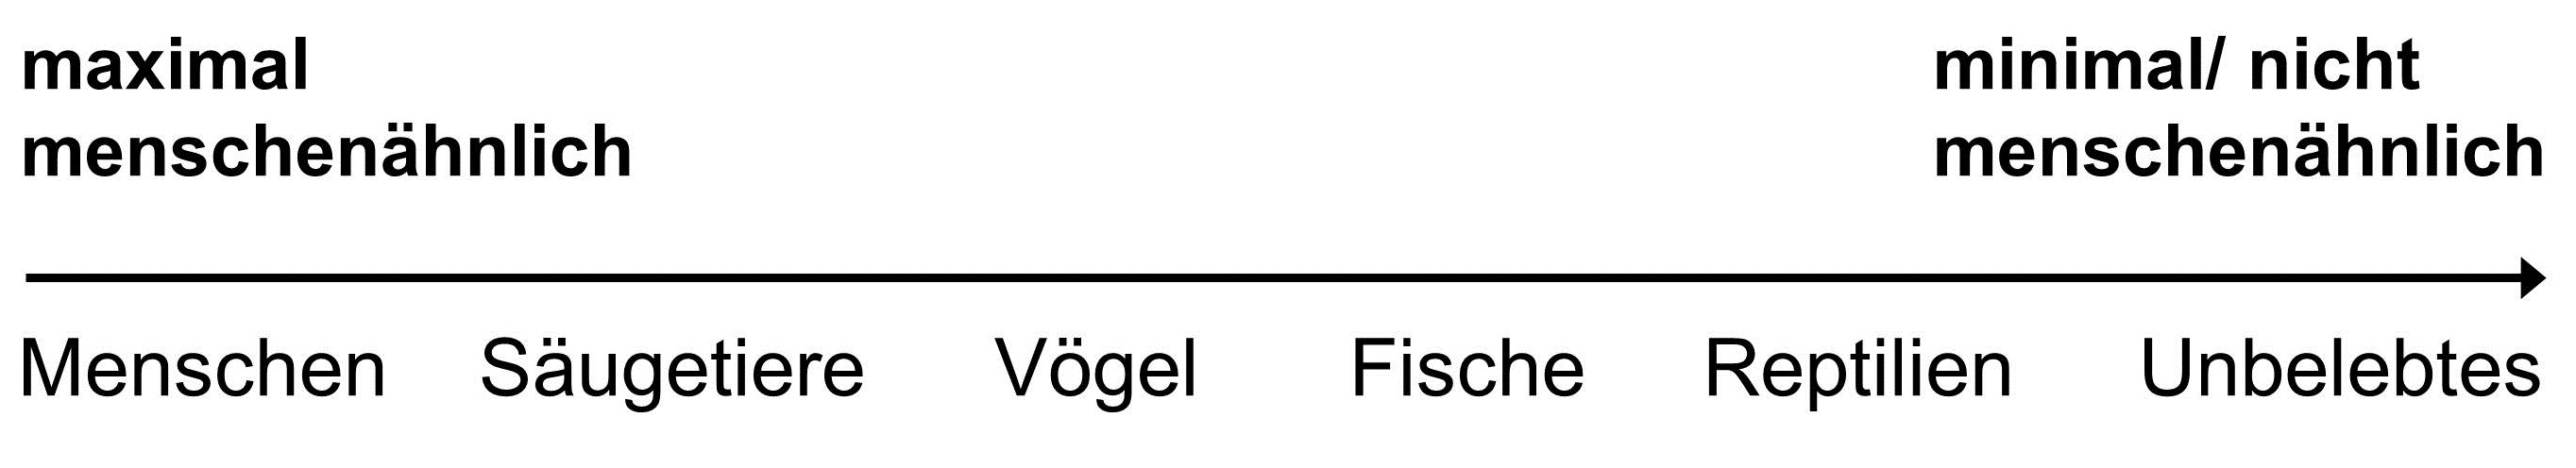
\includegraphics[width=10cm]{images/koepcke-anthro.jpg}
\caption {Antrophozentrisches Kontinuum \parencite[115]{Kopcke2000}}
\label{anthro}
\end{center}
\end{figure} 

 
\textcite{Enger2011} verbinden eine solche Hierarchisierung mit dem in der kognitiven Linguistik diskutierten \object{embodiment}-Konzept \parencite[vgl.][]{Lakoff1999}:
\blockcquote[208]{Enger2011}[.]{The hierarchy ranks entities as
closely or distantly related to humans, who use their bodily experience (among other things) as the basis for categorization. The observation that humans are different from animals probably presupposes our experience with our bodies as different from those of animals. It is hard to believe that the Animacy Hierarchy would make equally good sense if humans did not have (human) bodies} Nicht zuletzt sind es also ontologische Gemeinsamkeiten, die die Kategorisierung bedingen. Der Hund des Nachbarn ist uns ähnlicher als die Spinne im Wohnzimmer, die man nur bei genauem Hinsehen erkennt.
Mit unbelebten Entitäten haben wir noch weniger gemein, was kognitiv eine stärkere kategoriale Abgrenzung zur Folge hat  \parencite[vgl. auch][16]{Yamamoto1999}.

Belebtheit kann grammatische Systeme an unterschiedlichen Stellen \hervor{splitten} -- manche reagieren auf grobe Distinktionen wie belebt/unbelebt oder menschlich/nicht menschlich, andere spiegeln feinere Abstufungen wider. So kann z.B. bei menschlichen Referenten auch der Verwandtschaftsgrad oder das Geschlecht für die Wahl von Pronomina ausschlaggebend sein \parencite[s. ausführlich][194ff.]{Comrie1989, Corbett2000}. Es wurde außerdem gezeigt, dass diskursive Rollen (Sprecher,  Adressat und Referenten, über die gesprochen wird) oder die Art der Referenzierung (Pronomen, Eigennamen, Gattungsnamen)  mit unterschiedlichen Belebtheitsgraden assoziiert sind \parencite[s. etwa][186]{Comrie1989}. So stehen Pronomen, insbesondere in der ersten Person, an der Spitze der Belebtheitshierarchie,  da sie typischerweise auf Menschen referieren \parencite[s. auch][67]{Fraurud1996}; eine solche Korrelation ist bei Gattungsbezeichnungen nicht gegeben. 

Dies hat zur Erweiterungen der ursprünglich auf \textcite{Silverstein1976} zurückgehenden Belebtheitshierarchie geführt \parencite[vgl. u.a.][]{Allan1987,Langacker1991,Langacker2008,Dixon1995,Corbett2000,Foley2007}. Das gebräuchlichste Modell stammt von \textcite[85]{Dixon1995}, s. \REF{ex:dixon} \parencite[vgl.][130]{Croft2006}.\footnote{Um anzuzeigen, dass die linke Kategorie allem, was rechts folgt, hierarchisch übergeordnet ist, wird meist das Größer-als-Zeichen \hervor{>} verwendet. Allerdings gibt es auch Autoren, die hierfür \hervor{<} verwenden, z.B. \textcite{Allan1987,Croft2006}.}  

\begin{exe}
	\ex \label{ex:dixon} \object{Extended Animacy Hierarchy}: first/second person pronouns > third person pronoun > proper name > human common noun > non-human animate common noun > inanimate common noun
	\end{exe}
\noindent
Hierarchien wie diese werden u.a. bei Analysen von Numerussystemen genutzt \parencite{Corbett2000,Croft2006} und zwar mit dem Ziel, Generalisierungen in Form von \hervor{implikativen Unversalien} \parencite[2]{Zifonun2006} aufzustellen \parencite[vgl. auch][47]{Dahl1996}. Wenn beispielsweise Pronomen der 3. Person eine Singular-Plural-Distinktion aufweisen, dann ist zu erwarten, dass alle höherstehenden Kategorien in der Belebtheitshierachie, also die 1. und 2. Person, ebenfalls eine solche Distinktion aufweisen \parencite[129]{Croft2006}. Zusätzlich können Voraussagen darüber getroffen werden, welcher Ausschnitt der Belebtheitshierarchie sich in der Grammatik niederschlägt. So müssen Numerusdistinktionen laut des von \textcite[56]{Corbett2000} formulierten \hervor{Constraint of the Animacy Hierarchy on the singular-plural distinction} immer den linken Rand betreffen und damit die \object{belebtesten} Kategorien. Zwar werden Generalisierungen wie diese auf Grundlage synchroner Sprachvergleiche entwickelt, sie können aber auch auf diachrone Daten übertragen werden und Antworten auf Fragen zu Ursprung und Ausbreitung von grammatischen Kategorien liefern. \textcite[265ff.]{Corbett2000} vermutet etwa, dass die Grammatikalisierung von Numerusdistinktionen analog zum oben formulierten \hervor{Constraint} bei belebten Referenten beginnt. Die Idee, dass grammatische Innovationen wie Numerusdistinktion zunächst ganz bestimmte Belebtheitskategorien erfassen und sich dann entlang der Hierarchie ausbreiten, wird in Abschnitt \ref{sec:belebtwandel} in Bezug auf die Definitheit wiederaufgenommen. 

Wie \textcite[130]{Croft2006} zeigt, kombiniert die \object{Extended Animacy Hierarchy} drei Subhierarchien, s. \REF{ex:croft}.

\begin{exe}
	\ex \label{ex:croft}
	\begin{xlist}
		\ex \label{ex:person} \object{Person}: first, second > third
		\ex \label{ex:referenz} \object{Referentiality}\footnote{Anzumerken ist, dass der Term \object{Referentiality} \extrans{Referentialität} nicht die in der Referenzlinguistik diskutierte Zugänglichkeit des Referenten (fokussiert, aktiviert, bekannt etc.) \parencite[vgl. etwa][]{Gundel1993} betrifft, sondern  auf der Frage beruht, wie man ausdrucksseitig Monoreferenzialität garantiert kann.} pronoun > proper name > common noun
		\ex \label{ex:animacy} \object{Animacy}: human > animate > inanimate
	\end{xlist}
\end{exe}
\noindent
Insbesondere an der Personen-Hierarchie aus \REF{ex:person} wird deutlich, dass die Frage, inwiefern wir uns mit einer Entität identifizieren, in das Belebtheitskonzept hineinspielt \parencite[10f. u. 25f.]{Yamamoto1999}. \textcite[307f.]{Langacker1991} bevorzugt vor diesem Hintergrund den Ausdruck \object{Empathie}-Hierarchie \parencite[ebenso][]{Lehmann2004a}. An der Spitze steht der von seinen Emotionen und kommunikativen Zielen geleitete Sprecher selbst. Gefolgt wird er vom Hörer, dessen hoher Empathiegrad sich durch seine Anwesenheit im Diskurs begründet und dem damit zusammenhängenden Potential, unmittelbar Einfluss auf den Diskurs und den Sprecher auszuüben.  Weil Sprecher und Hörer im Normalfall menschlich sind\footnote{Es ist auch vorstellbar, dass ein höher gestelltes Tier wie z.B. ein Hund der Adressat ist.}, variieren die eigentlichen Belebtheitsgrade (s. \ref{ex:animacy}) nur bei der dritten Person. Ihre Rangfolge entspricht ebenfalls einem Empathiegefälle. 

Bei der Referentialitätshierachie in \REF{ex:referenz} fließt der Faktor Individualität mit ein \parencite{Timberlake1977,Hopper1980,Dahl1996,Fraurud1996,Yamamoto1999}, der vor allem an der Unterscheidung Eigennamen und Gattungsname (Appellativum) sichtbar wird, s. auch Abschnitt \ref{sec:indi}.\footnote{Zum indiviualitätsstiftenden Potential von Pronomen, s. \textcite[29ff.]{Yamamoto1999}. Pronomen verweisen typischerweise auf menschliche Referenten, die im Kurzzeitgedächtnis aktiviert sind, und liefern Informationen zu Numerus, Geschlecht, sozialem Status u.ä., was die Individualität des Referenten hervorhebt.} Eigennamen wie \object{Thomas} sind monorefentiell und verweisen auf bekannte und damit hoch individualisierte Referenten. Bei Gattungsbezeichnungen, etwa \object{der Abteilungsleiter}, verläuft das Referieren über einen semiotischen Umweg, und zwar indem die Bedeutung von \object{Abteilungsleiter} einem passenden Referenten zugewiesen wird. Der Individualitätsgrad ist dann geringer, weil der Referent über seine Rolle im Unternehmen definiert wird.

Es ist anzumerken, dass hierarchische Gliederungen wie diese nicht suggerieren sollen, dass die entsprechenden Kategorien linear und klar voneinander abgrenzbar sind. Dies wird  insbesondere bei metaphorischer oder metonymischer Sprache sowie bei jeder Form der Personifizierung sichtbar \parencite[vgl.][62]{Dahl1996}. Die Beispiele in \REF{ex:borderlines} führen Grenzfälle und Überschneidungen entlang der Belebtheithierarchie auf \parencites()()[basierend auf][62f.]{Dahl1996}[18ff]{Yamamoto1999}. Sie verdeutlichen, dass Belebtheit auch vom Kontext abhängig ist und neben der Empathie auch Faktoren wie Agentivität und Relevanz den Belebtheitsgrad determinieren (vgl. hierzu ausführlich: Abschnitt \ref{sec:partizipanten} und \ref{sec:relevanz}).

So müsste \object{Natur} oder \object{Berlin} ohne Kontext als \object{unbelebt} klassifiziert werden. Im übertragenen Gebrauch (s. \ref{ex:metapher} und \ref{ex:metonymie}) denotieren sie jedoch Referenten, die denken, fühlen oder handeln; es sind \blockcquote[62]{Dahl1996}{non-personal agents}. Das gleiche gilt für vermenschlichte Gegenstände, s. \REF{ex:anthropo} \parencite[vgl. auch][]{Epley2007}. Mythologische Figuren, s. \REF{ex:mytho}, oszillieren zwischen \object{abstrakt} und \object{belebt}, denn sie agieren menschlich, haben aber dennoch keine feste Gestalt wie Menschen. Weil sie kulturell einen hohen Stellenwert einnehmen, sind sie kognitiv besonders auffällig. 
  
\begin{exe}
	\ex \label{ex:borderlines}
	\begin{xlist}
		\ex \label{ex:metapher} Metaphern (\object{Die Natur ist großzügig.})
 		\ex \label{ex:metonymie} Metonymien: (\object{Berlin stimmt dem Entschluss der EU zu.})
		\ex \label{ex:anthropo} Anthropomorphe Tiere oder Gegenstände \\(z.B. Haustiere, Puppen, humanoide Roboter)	
		\ex \label{ex:mytho} Mythologische Figuren (\object{Gott}, \object{der heilige Geist})
	\end{xlist}
\end{exe}
\noindent
Auf Grundlage solcher Überlegungen modelliert \textcite{Yamamoto1999} ein Prototypenmodell, das die genannten Grenzfällen beinhaltet und die graduellen Übergänge innerhalb der Hierarchien repräsentieren soll, s. Abbildung \ref{yamamoto}. Die durchgezogenen Linien, welche von der quadratisch-abgegrenzten Mitte ausgehen, führen zu Referenten mit gleichem Belebtheitsgrad; die gestrichelten Linien verweisen auf geringere Belebtheitsstufen.

\begin{figure}[h]
\begin{center}
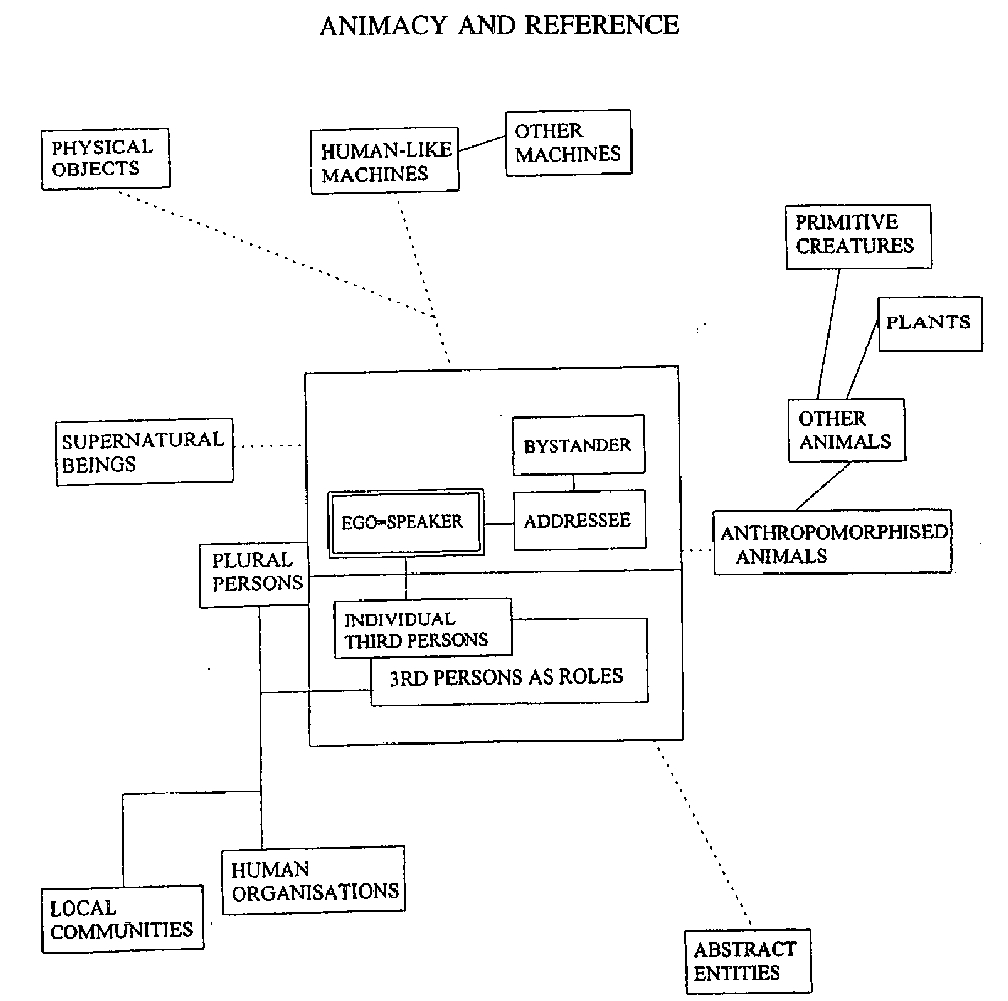
\includegraphics[width=12cm]{images/yamamoto2.jpg}
\caption {Belebtheitskategorien als Prototypenmodell \parencite[aus][38]{Yamamoto1999}}
\label{yamamoto}
\end{center}
\end{figure} 


Im Zentrum des Prototypenmodells in Abb. \ref{yamamoto} stehen belebte Entitäten, die nach Person (\textsc{Speaker, Addressee, Bystander}) und Referenzausdruck (vgl. die Skalen \ref{ex:person}  und \ref{ex:referenz} oben) weiter unterteilt sind. Nicht mehr dem prototypischen Kern zugehörig sind menschliche Referenten, die eine geringe Individualität aufweisen, z.B. weil sie nicht alleine, sondern in der Mehrzahl agieren (\textsc{Plural Persons}) oder als Kollektiv auftreten (\textsc{Human Organisations, Local Communities}); auf die Korrelation von Individualität und Belebtheit wird noch ausführlich in Abschnitt \ref{sec:indi} eingegangen. In die Peripherie gehören neben übernatürlichen Entitäten mehr oder weniger vermenschlichte Tiere und Konkreta.  

Darüber hinaus verortet Yamamoto abstrakte Entitäten außerhalb des Prototypenzentrums. Eine Erweiterung der Belebtheitshierarchie um diese Kategorie nehmen auch \textcite{Allan1987,Langacker1991,Croft1995} vor; \textcite[194]{Enger2011} gruppieren \object{Abstrakta} bzw. \object{Abstractions} und \object{Massennomen}, s. \REF{ex:einfachbelebt} (als Erweiterung der Hierarchie aus \ref{ex:animacy}).

\begin{exe}
	\ex \label{ex:einfachbelebt} \textsc{human > animate > inanimate  > abstracts and massnouns}
	\end{exe}
\noindent
Für den geringen Belebtheitsgrad dieser Kategorien muss neben ihrer Unähnlichkeit zum Menschen noch ein weiterer Parameter verantwortlich sein. Denn Massennomen   ließen sich auch unter die unbelebten Konkreta subsumieren, etwa \object{Gold}, so dass die Unbelebtheit allein die niedrige Platzierung auf der Skala nicht rechtfertigt. Was Massennomen von anderen unbelebten Objekten wie \object{Diamant} unterscheidet, ist ihre unscharfe Kontur und damit das Kriterium der konzeptionellen Begrenztheit \parencite[203ff.]{Langacker1987}. Das gleiche gilt für Abstrakta wie \object{Friede}. Im Gegensatz zu Konkreta sind sie nicht-materiell. Nach \textcite[197]{Comrie1989} differenzieren die meisten Sprachen morphologisch nicht innerhalb der Kategorie \textsc{inanimate}\footnote{Eine Ausnahme ist die Sprache der Navahos, einem Stamm Nordamerikas, in der Entitäten wie \object{Wind}, die als Verursacher einer Handlung auftreten können, durch ein spezielles Präfix von anderen unbelebten Objekten abgegrenzt  werden \parencite[197]{Comrie1989}, wobei man hier fragen müsste, ob eine solche Markierung nicht besser als Ausdruck der semantischen Rolle \object{Force} \parencite[73]{Primus2012} betrachtet werden sollte.}, so dass Abstrakta in groben Belebtheitsdistinktionen unter die Konkreta fallen.

In Bezug auf den Definitartikel tragen Abstrakta und Massennomen allerdings eine besondere Rolle, denn sie gehören zu den Kategorien, die -- später als quantifizierbare Konkreta -- mit einem sich entwickelnden Artikel determiniert werden, vgl. für das Althochdeutsche \textcite{Oubouzar1992} und \textcite{Szczepaniak2011}, für das Altspanische \textcite{Company1991}  oder für das Altgriechische \textcite{Napoli2009}. Auch im Gegenwartsdeutschen können sie in bestimmten Kontexten ohne Artikelwort gebraucht werden, z.B. \object{Sie kauft Gold},  \object{Wir warten auf Frieden} oder \object{Er hat Vertrag} \parencite{DAvis2013}, aber \object{*Sie kauft Haus}, \object{*Wir warten auf Brief}, \object{*Er hat Schreibtisch}. Aus diesen Beobachtungen lässt sich schließen, dass Belebtheit sowie damit zusammenhängend die Individualität zentrale Einflussfaktoren für die Ausbreitung des Defintitartikels ist. 

\section{Belebtheitsgesteuerter Wandel des Definitartikels}\label{sec:belebtwandel}

Im Folgenden wird dafür argumentiert, dass die Entwicklung des Definitartikels entlang der Belebtheitshierarchie verläuft. Dass Belebtheit nicht nur synchrone Variation, sondern auch diachronen Wandel determinieren kann, belegen eine Reihe von Studien \parencite[vgl. die Übersicht in][]{Enger2011}. Für das Deutsche hat \textcite{Kopcke1995, Kopcke2000a,Kopcke2000,Kopcke2005} gezeigt, dass die semantische Remotivierung der schwachen Maskulina (z.B. \object{der Matrose, des Matrosen})  durch den  Belebtheitsgrad des Referenten gesteuert wurde. Die stete Abwanderung unbelebter Referenten aus dieser Deklinationsklasse hat dazu geführt, dass schwache Maskulina heute belebten Referenten vorbehalten sind. 
Auch der Stellungswandel des adnominalen Genitivs, der die Expansion des Definitartikels fördert (s. Abschnitt  \ref{sec:genitiv}), ist belebtheitsgesteuert \parencite[215-223]{Demske2001}: NPs mit unbelebten Referenten tendieren seit dem späten Althochdeutschen zur Nachstellung, während belebte Referenten noch bis ins frühe 17. Jh. pränominal erscheinen (etwa: \object{des Fürsten Gewand}). Im Gegenwartsdeutschen werden hingegen in erster Linie Eigennamen und damit typischerweise menschliche Referenten vorangestellt  (\object{Pauls Auto}).   

Die Entwicklung der satzinternen Großschreibung \parencite{Bergmann1998,Bergmann1998a,Bergmann1999,Szczepaniak2011,Szczepaniak2016} ist ein weiteres Beispiel für belebtheitsgesteuerten Wandel. Wie die Abbildung in \ref{sgs} zeigt, exponiert die Majuskel zu Beginn vor allem belebte und stark individuierte Entitäten (insbesondere Personennamen) und erfasst erst zum Ende des 16. Jh. regelmäßig unbelebte Konkreta. Abstrakta werden erst Ende des 17. Jh. in der großen Mehrheit großgeschrieben.   

\begin{figure}
\begin{center}
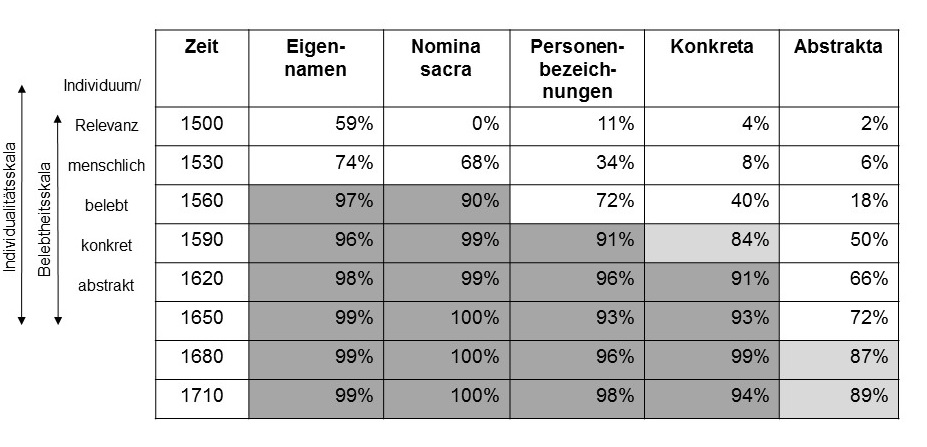
\includegraphics[width=12cm]{images/SGS-bergmann-szczepaniak-neu.jpg}
\caption {Die Durchsetzung der satzinternen Großschreibung im Deutschen (\cite{Bergmann1999}, zitiert aus \cite[351]{Szczepaniak2011})}
\label{sgs}
\end{center}
\end{figure} 

Die Forschung zum Definitartikel spricht dafür, dass die Ausbreitung des Artikels in ähnlicher Weise vonstatten ging. So dokumentiert \textcite[73ff.]{Oubouzar1992} aufbauend auf einer früheren Korpusuntersuchung \parencite{Oubouzar1989}, dass das  Artikelwort \object{dër} am Anfang (im ahd. Isidor) ebenfalls primär bei belebten (und diskursrelevanten) Referenten erscheint \parencite[vgl. insbesondere][566-567]{Oubouzar1989} und erst zum Ende des Ahd. auch vermehrt Abstrakta erfasst \parencite[][572]{Oubouzar1989}; neben Unika und generischen NPs, die in Abschnitt \ref{sec:definitartikel} bereits diskutiert wurden. \textcite[74ff.]{Szczepaniak2011} nimmt basierend auf diesen Beobachtungen und durch die Analyse von Stichproben aus der ahd. Sprachperiode eine belebtheitsgesteuerte Ausbreitung des Artikels an und zwar entlang der Kategorien \textsc{belebt > unbelebt > abstrakt}. Was allerdings bislang noch fehlt, ist eine Korpusuntersuchung, welche die Korrelation von Belebtheit und \object{dër}-Setzung systematisch offenlegt. 

In der Sprachtypologie wird zwar auf das Zusammenspiel von hohem Belebtheitsgrad und Definitheit verwiesen \parencites()()[s. z.B.][53]{Dahl1996}[][166f.]{Croft2006}.\footnote{Definitheit kann in Kombination mit Belebtheit beispielsweise für \object{differential object marking} (= DOM) sorgen \parencite{Aissen2003}. \textcite{Lyons1999} liefert hierfür eine Erklärung \parencite[ähnlich argumentiert auch][119]{Croft1995}: \blockcquote[2014]{Lyons1999}{The operation for the hierarchy in some processes (most notably object marking and verb-object agreement) has been accounted for functionally, in terms of a natural tendency for the subject or agent to be more animate and more definite than the object or patient. Deviation from this natural pattern are then marked morphologically}.}
Dies wird schon deutlich,  wenn man die ersten drei Kategorien der \object{Extended Animacy Hierarchy} in \REF{ex:dixon} betrachtet: Pronomen in der 1. Person sind naturgemäß definit, ebenso Eigennamen. Beide Formen referieren typischerweise auf Menschen. Dass die Ausprägung der Definitheitskategorie selbst, d.h. die  Markierung durch einen Artikel, ein Reflex belebtheitsbedingter Konzeptualisierung sein könnte, wird jedoch kaum diskutiert. Eine Ausnahme ist die Arbeit von \textcite{Enger2011}, in der die Frage aufgeworfen wird, von welcher Belebtheitsklasse aus die Kategorie Definitheit (in Form eines sich entwickelnden Artikelwortes\footnote{Zu weiteren Möglichkeiten, Definitheit auszudrücken vgl. Abschnitt \ref{sec:def-ahd}.}) ihren Anfang nimmt und über welche Kategorien die Expansion erfolgt. Zur Beantwortung formulieren \textcite[206]{Enger2011} ein sog. \hervor{Relevance Constraint}, das nicht nur für die Definitheit, sondern auch für die Nominalkategorien Kasus, Numerus und Genus gelten soll, s. \REF{ex:enger}. 
   
\begin{exe}
	\ex \label{ex:enger} Language change targets the part of the lexicon where the categories in question are most relevant for human experience.
	\end{exe}
\noindent
Das \object{Constraint} bezieht sich auf die Belebtheitshierarchie aus \REF{ex:einfachbelebt}, die auf einer vertikalen Achse mit belebten Referenten beginnt und am unteren Ende Abstrakta und Massennomen anführt, s. \ref{enger};  Referenten von Eigennamen als \hervor{belebteste} Klasse ergänzen die Skala. Pronomen kommen als mögliche Belebtheitskategorie nicht in Frage, da diese nicht durch einen Definitartikel erweiterbar sind. 

\begin{figure}[h]
\begin{center}
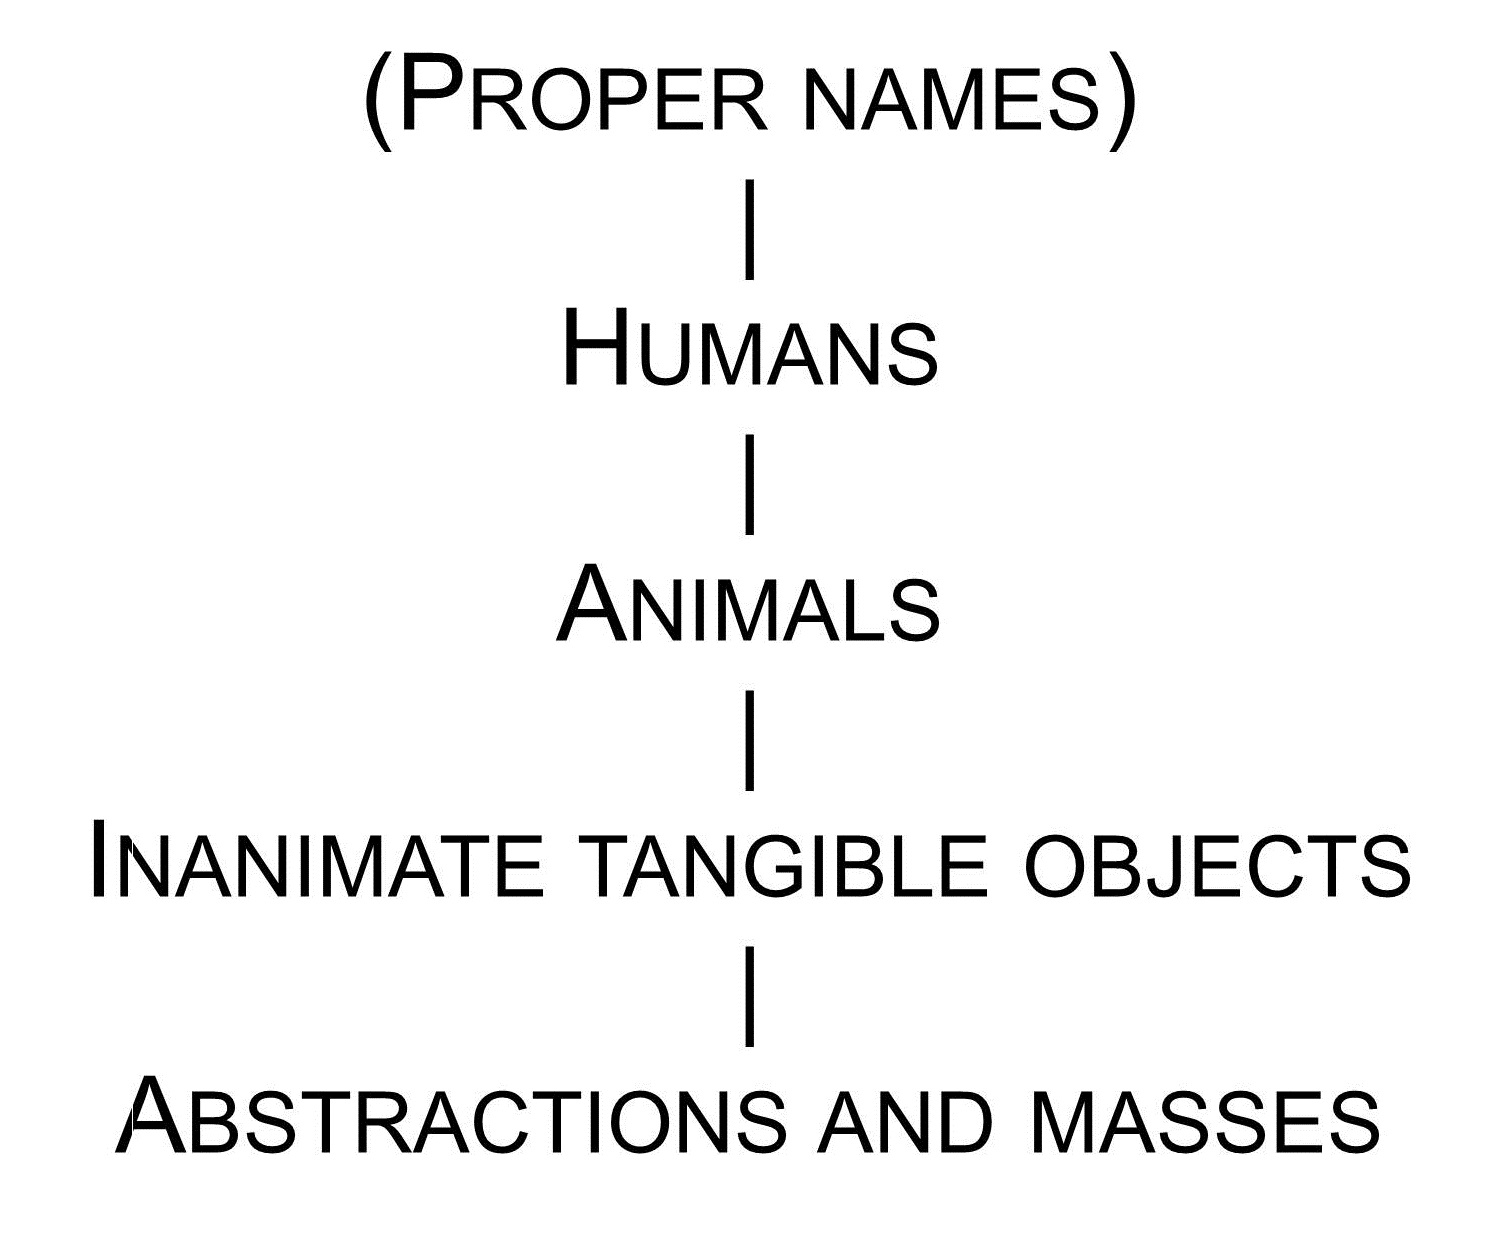
\includegraphics[width=5cm]{images/enger-hierarchie.jpg}
\caption {Die Belebtheitshierarchie nach \textcite{Enger2011}}
\label{enger}
\end{center}
\end{figure} 
	

Während nach \textcite[206ff.]{Enger2011} Numerus- und Genusmarkierungen für den Kopf der Hierarchie relevant sind und Kasusmarkierungen sowohl am oberen wie am unteren Ende ihren Ursprung finden, startet Definitheit von der Mitte der Hierarchie, nämlich bei konkreten Referenten, auf die man mit einem Gattungsnamen referiert.  Als Begründung führen die Autoren an, dass Definitartikel \blockcquote[205]{Enger2011}[.]{are used when the speaker assumes that the addressee is able to identify the referent. Since countable concrete nouns are prototypical referents, definiteness is most relevant for such nouns}. Man muss die Begründung präzisieren: Die Definitheit ist nicht deswegen relevant, weil Konkreta prototypische Referenten sind, sondern weil die Information identifizierbar/nicht-identifizierbar bei dieser Substantivklasse kommunikativ wichtig ist. Im Vergleich zu Eigennamen wird dies besonders deutlich: Wenn ein Referent mit einem Eigennamen denotiert wird, präsupponiert dies, dass der Referent bekannt ist \parencite[997]{Heim2011}. Daher ist die Determinierung mit dem Definitartikel zum Zwecke der eindeutigen Referenzierung redundant. Der onymische Artikel ist aus diesem Grund erst zu einer späteren Entwicklungsstufe zu erwarten. Die Untersuchungen von \textcite{Schmuck2014,Schmuck2020} belegen den Artikelgebrauch bei Personennamen seit dem 16. Jh. in süd-östlichen Sprachregionen und zwar aus pragmatischen Gründen, etwa zum emphatischen Verweis oder zur Denunzierung von Referenten.

In Bezug auf das Altspanische kann \textcite[421]{Company1991} empirisch belegen, dass der Definitartikel zuerst bei zählbaren Konkreta, etwa \object{Spiegel} oder \object{Schwert} erscheint und begründet dies folgendermaßen: \blockcquote[421]{Company1991}{[S]u naturaleza semántica -- ser  concretos y con límites -- era acorde
con uno de los valores del artículo, el de dar referencia, concretar y aproximar
entidades. (sinngemäß: \extrans{Ihre Semantik -- konkret und begrenzt zu sein -- stand in Übereinstimmung mit der Funktion des Artikels, nämlich zu referieren, zu konkretisieren und Referenten in den Vordergrund zu stellen.})} Hier wird also auf die semantische Kompatibilität von Substantivklasse und Definitartikel verwiesen:  Wenn der Definitartikel dazu gebraucht wird, einen Referenten von anderen potentiellen Referenten kognitiv abzugrenzen, dann ist ein solcher Abgrenzungsprozess besonders für außersprachliche Entitäten geeignet, die von sich aus eine scharfe Kontur haben und gegenständlich sind.

Im frühen Stadium seiner Entwicklung hat der Definitartikel, wie \textcite{Epstein1993,Epstein1994} am Beispiel des altfrz. \object{le/la} zeigt, zudem die Funktion, Diskursreferenten pragmatisch hervorzuheben. Hierfür kommen vor allem menschliche Referenten in Frage, da sie wegen ihrer ontologischen Eigenschaften häufig eine besondere Hervorhebung verdienen: Sie sind kognitiv auffälliger als unbelebte Referenten und treten häufig als Agens in Erscheinung, was ihre kommunikative Relevanz für die Diskursteilnehmer erhöht. Die Auszeichnung von Menschen mit einem Artikelwort steht im Dienste der Expressivität, die auch für andere Sprachwandelprozesse, etwa den Negationswandel \parencite{Jager2008}, eine Triebfeder ist: Die Information, dass ein Referent eine hohe Dikursprominenz hat, soll möglichst deutlich markiert werden. Ein genuin demonstratives Artikelwort ist hierfür prädestiniert (vgl. hierzu auch die Ausführungen in Abschnitt \ref{sec:kata}).

Menschen bzw. konkrete Referenten bilden also -- so die Hypothese -- den Startpunkt der Artikelentwicklung, während die Klasse der Abstrakta und Massennomen undeterminiert bleiben. \textcite{Epstein1994} begründet diese Situation im Rahmen der kognitiven Linguistik folgendermaßen: \blockcquote[71]{Epstein1994}{Concrete count nouns tend to be construed as definite more frequently than
abstract or mass nouns, which are more likely to be construed as generic.
These tendencies are not surprising, given that concrete count nouns represent
entities that are cognitively more salient than abstract nouns and more
easily individuated than mass nouns. These entities are therefore more
likely to be construed as referential, as active participants in a scene, and as figure rather than ground. Conversely, since abstract and mass nouns have
a lower degree of individuation, they are more likely to be construed as
non-referential, background entities.} 

Der konzeptionelle Unterschied zwischen den Substantivklassen ist nach Epstein also eine Frage der \object{Individualität}. Man kann die Hypothese aufstellen, dass Referenten, die von sich aus einen hohen Individualitätsgrad aufweisen,  besonders affin gegenüber einer Kennzeichnung mit dem Definitartikel sind, weil dieser selbst eine individualisierenden Effekt auf Referenten hat. Ein Belebtheitsmodell, das die Expansionsschritte des Definitartikels abbilden soll, muss also über die Hierarchie \textsc{menschlich > belebt > unbelebt} hinausgehen und Parameter der Individualität mit einbeziehen. 

\section{Belebtheit und Individualität}\label{sec:indi}

Die Individualität erfasst, inwiefern ein Objekt sich von seiner Umgebung und anderen Entitäten abgrenzt und somit als Individuum wahrgenommen wird \parencite{Timberlake1975,Timberlake1977, Hopper1980,,Fraurud1996, Szczepaniak2011}. Die Kennzeichnung mit einem Eigennamen ist die einfachste Art, einen hohen Individualitätsgrad zu sichern, weswegen Menschen als prototypische Individuen obligatorisch einen Eigennamen tragen \parencite[71]{Fraurud1996}. Prinzipiell können aber auch nicht menschliche  oder sogar abstrakte Entitäten mittels Eigennamen individuiert werden, etwa Haus\-tiere oder Puppen, aber auch Autos und Küchengeräte\footnote{\url{https://www.chefkoch.de/forum/2,22,447655/Haben-eure-Kuechengeraete-Namen.html}, zuletzt aufgerufen am 21.02.2020.} oder Sturmtiefs \parencite{Nubling2012}. Daran wird deutlich, dass Individuiertheit und Belebtheit orthogonal zueinander laufen. In Bezug auf die für den Definitartikel relevanten Gattungsnamen lässt sich allerdings zeigen, dass hohe Belebtheit mit hoher Individualität korreliert: Menschen als typische Agens beanspruchen einen größeren Handlungsraum und aktivieren ein im Vergleich zu unbelebten Dingen höheres Maß an Empathie \parencite{Langacker1991}. Dies macht sie zu kognitiv auffälligen Entitäten, was der Individualität förderlich ist. Daneben gibt es noch weitere Parameter, die einen Einfluss auf die Individualität haben, s. Tabelle \ref{tab:indi}. Sie bedingen sich zum Teil gegenseitig: So sind Eigennamen immer referentiell und definit\footnote{Eine Ausnahme sind Gattungslesarten von Eigennamen wie in \object{Einen Schweinsteiger gibt es nur einmal}.} und nur Entitäten, die zählbar sind, können auch eine Numerusopposition aufweisen. 

\begin{table}[h]
\begin{tabular}{ll}
\lsptoprule
Individuiert & Nicht-individuiert\\ \midrule
Eigenname                    & Gattungsname         \\
Mensch, belebt               & unbelebt             \\
konkret                      & abstrakt             \\
Singular                     & Plural               \\
zählbar                      & nicht zählbar        \\
referentiell, definit        & nicht-referentiell   \\ \lspbottomrule
\end{tabular}
\caption{Faktoren für die Individualität \parencite[253]{Hopper1980}\label{tab:indi}}
\end{table}

Die tabellarische Einteilung geht ursprünglich zurück auf \textcite{Timberlake1975,Timberlake1977} und wird vor allem als Maß für Transitivitätseffekte genutzt, wobei ein individuiertes Objekt die Transitivität eines Satzes erhöht \parencite[s. auch][]{Gillmann2016}. Je mehr Eigenschaften ein Objekt aus der linken Spalte von Tabelle \ref{tab:indi} aufweist, umso näher kommt es dem prototypischen Individuum. Die Beispiele in \REF{ex:stossen} illustrieren das Zusammenspiel von Belebtheit, Individualität und Transitivität (Beispiele aus \cite[253]{Hopper1980} und daran anknüpfend \cite[344]{Szczepaniak2011}).


\begin{exe}
	\ex \label{ex:stossen}
	\begin{xlist}
		\ex \label{ex:stuhl} \object{Ich stieß gegen den Stuhl.}
 		\ex \label{ex:kundin} \object{Ich stieß gegen die Kundin.}
		\ex \label{ex:chalie} \object{Ich stieß gegen Charlie.}
	\end{xlist}
\end{exe}
\noindent
In \REF{ex:stuhl} liegt die Aufmerksamkeit auf dem Agens \object{ich}. Man geht nicht davon aus, dass das (unbelebte) Patiens \object{Stuhl} beim  Zusammenstoß Schaden genommen hat; der Stuhl wurde nur minimal affiziert. Der Transitivitätseffekt ist in \REF{ex:kundin} viel höher. Es ist wahrscheinlich, dass \object{der Kundin} ebenso wie dem Verursacher beim Zusammenstoß etwas passiert ist. Die Empathie und damit auch die Individualität steigt bei Menschen, die bekannt sind und deswegen mit einem Eigennamen ausgestattet werden können, vgl. \REF{ex:chalie}.

Nachfolgend werden die Kategorien aus Tabelle \ref{tab:indi} erläutert und Korrelationen zum Definitartikelgebrauch offengelegt. 

\subsection{Der Definitartikel als \hervor{Individualisierer}} \label{sec:individualisierer} 

Unter der Opposition \object{referentiell, definit} vs. \object{nicht-referentiell} verstehen \textcite{Hopper1980} den Grad der Identifizierbarkeit eines Referenten und den damit verknüpften sprachlichen Mitteln. Der Definitartikel als Marker für Identifizierbarkeit sorgt dafür, dass ein Referent an Individualität gewinnt -- im Gegensatz zum Indefinitartikel --, s. \REF{ex:Referentialität}. Entsprechend kann ein Massennomen durch den Definitartikel eine individualisierte Lesart erhalten, wie \textcite[253]{Hopper1980} an den Beispielen in \REF{ex:bier} (hier übersetzt aus dem Englischen) illustrieren \parencite[vgl. auch][257]{Leiss2000}.

\begin{exe}
	\ex \label{ex:Referentialität} \object{Ich habe einen/den Film gesehen.}
	\ex \label{ex:bier} \object{Fritz trank ein wenig/das Bier.}
\end{exe} 
\noindent
Bei Objektinkorporierungen liegt immer ein nicht-referentieller Gebrauch des Substantivs vor, s. \REF{ex:rad} \parencite[vgl. u.a.][]{Mithun1984}. Der Definitartikel hebelt diese Lesart aus, indem er eine eindeutige Referenzierung erzwingt und eine Inkorporierung blockiert, s. \REF{ex:dasrad}.  Einen ähnlichen Effekt kann man bei unspezifischen Nominalphrasen beobachten, s. \REF{ex:unspez}. Die Auflösung der speziellen Klise in \REF{ex:schule}, führt dazu, dass der Referent als eine bestimmte \object{Schule} identifiziert und damit individualisiert wird, s. \REF{ex:dieschule}. Wie \textcite[169]{Croft2006} zeigt, sind es sprachübergreifend in erster Linie unbelebte Referenten, die inkorporiert werden, so dass Nicht-Referentialität sowohl mit Definitheit als auch mit Belebtheit negativ korreliert.

\begin{exe}
	\ex \label{ex:inkorp}
	\begin{xlist}
		\ex \label{ex:rad} \object{Sie fährt Fahrrad.}
		\ex \label{ex:dasrad} \object{?Sie fährt das rote Rad.}
	\end{xlist}
	\ex \label{ex:unspez}
	\begin{xlist}
		\ex \label{ex:schule} \object{Er geht noch zur Schule.}
		\ex \label{ex:dieschule} \object{Sie geht noch zu der Schule, die...}
	\end{xlist}
\end{exe} 

Wenn der Definitartikel selbst eine individualisierende Funktion hat, ist es wahrscheinlich, dass ein hoher Individualitätsgrad die Definitartikelsetzung begünstigt. Neben der Belebtheit sind es der Konkretheitsgrad (\object{konkret-abstrakt}), der Numerus (\object{Singular-Plural}) und die Zählbarkeit (\object{zählbar-nicht zählbar}), die 
die Individualität determinieren, vgl. Tabelle \ref{tab:indi}.

\subsection{Konkreta vs. Abstrakta}\label{sec:konabst}

Konkrete Entitäten (etwa \object{Studentin, Hund, Stein, Kuchen}) weisen typischerweise klare Konturen auf und sind empirisch wahrnehmbar. Durch ihre Materialität grenzen sie sich maximal von ihrer Umwelt ab \parencite[344]{Szczepaniak2011}. Im Gegensatz dazu sind Abstrakta (z.B. \object{Treue, Glück}) nicht-materiell und haben keine scharfe Kontur. Es sind Einheiten, deren Bedeutung erst durch einen Abstraktionsprozess zustande kommt \parencite[279]{Ewald1992}. Weil Kinder diese Abstraktionsfähigkeit erst erlernen müssen, erwerben sie Wörter für Abstrakta später als Wörter für konkrete Referenten \parencite[396]{Bergelson2013}. Die konzeptionellen Unterschiede zwischen Konkreta und Abstrakta werden auch durch Studien aus der Kognitions- und Neurowissenschaft gestützt. Primingexperimente zeigen, dass beim Prozessieren von konkreten Referenten partiell andere Hirnareale aktiviert werden als bei abstrakten Stimuli \parencite{Binder2005,Weiss2013}; Aphasien beeinträchtigen kognitive Funktionen wie Memorieren und Wiederholen bei Abstrakta stärker als bei Konkreta \parencite{Moss1995,Moss1997}.

Die Duden-Grammatik gibt einen guten Überblick über typische abstrakte Entitäten und ihre Hyperonyme, s. \REF{ex:abstrakta} \parencite[146f.]{Duden2009}; weitere Beispiele zu diesen Gruppen liefert \textcite[143]{Schrauf2011}.

\begin{exe}
	\ex \label{ex:abstrakta}
	\begin{xlist}
		\ex \label{ex:vorstellung} Menschliche Vorstellungen: \object{Geist, Seele}
		\ex \label{ex:handlungen} Handlungen: \object {Schlag, Wurf, Schnitt, Boykott}
		\ex \label{ex:vorgang} Vorgänge: \object{Leben, Sterben, Schwimmen, Schlaf, Reise}
		\ex \label{ex:zustand} Zustände: \object{Friede, Ruhe, Angst, Liebe, Alter}
		\ex \label{ex:eigenschaft} Eigenschaften: \object{Würde, Verstand, Ehrlichkeit, Krankheit, Dummheit, Länge}
		\ex \label{ex:verhaeltnise} Verhältnisse oder Beziehungen: \object{Ehe, Freundschaft, Nähe, Unterschied}
		\ex \label{ex:wissenschaft} Wissenschaften und Künste: \object{Biologie, Mathematik, Musik, Malerei}
		\ex \label{ex:zeit} Maß- und Zeitbegriffe: \object{Meter, Watt, Gramm, Jahr, Stunde, Mai}
	\end{xlist}
\end{exe} 

Versucht man die Dichotomie \object{konkret-abstrakt} auf den Substantivwortschatz anzuwenden, stößt man schnell auf Abgrenzungsprobleme. So findet man den für Abstrakta definitorischen Prozess der Abstraktion auch bei Konkreta: Beispielsweise liegt \object{Kleidungsstück} auf einer höheren Abstraktionsstufe als \object{Kleid}\footnote{Auch diese Unterschiede lassen sich neurologisch nachweisen \parencite[s.][]{Ghio2013}.} \parencite[274]{Ewald1992}. Auch eine Sammelbezeichnung wie \object{Menschheit} ist das Resultat einer Abstraktion, die mit gleichzeitiger Verminderung des Be"-lebt"-heits- und In"-dividualitätsgrades einhergeht (dies wird sichtbar im Vergleich zu \object{Menschen} als alternative Gruppenreferenz). \object{Menschheit} ist aber dennoch \hervor{belebter} als eine Eigenschaft wie \object{Ehrlichkeit}. Deverbale Abstrakta wie \object{Verschmutzung} oder \object{Wurf} haben empirisch wahrnehmbare Grenzen und sind damit stärker konturiert als ein Massennomen wie \object{Gold}. Das Prototypenmodell von \textcite[279f.]{Ewald1992} versucht Grenzfälle wie diese zu erfassen, indem auch periphere Fälle zwischen den Polen \object{konkret} und \object{abstrakt} einbezogen werden, s. Abbildung \ref{abb:schrauf-ewald}. 

\begin{figure}[h]
\begin{center}
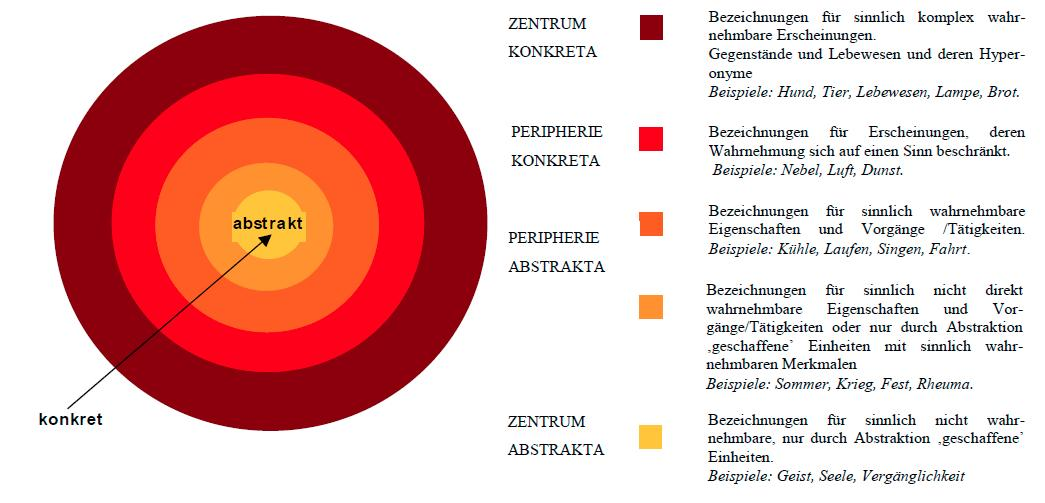
\includegraphics[width=12cm]{images/schrauff-ewald-neu.jpg}
\caption {Zentrum und Peripherie bei Konkreta und Abstrakta \parencite[][41]{Schrauf2011}}
\label{abb:schrauf-ewald}
\end{center}
\end{figure}


\textcite{Schrauf2011} zeigt allerdings, dass Ewalds Einteilung, die partiell auf Art und Anzahl der beteiligten Sinne beruht, nicht unproblematisch ist. So kann \object{Nebel} bpsw. nicht nur visuell, sondern auch taktil oder trigeminal wahrgenommen werden. Generell basiert die Wahrnehmung meist auf dem Zusammenspiel mehrerer Sinne. Selbst periphere Abstrakta wie \object{Fest} enthalten Komponenten, die eindeutig sinnlich wahrnehmbar sind, z.B. \object{tanzen, essen, trinken} etc. \parencite[vgl.][41]{Schrauf2011}. 

Eine Möglichkeit, das Modell zu ergänzen, wäre zwischen körpernahen und körperfernen Sinnen zu unterscheiden, wie es \textcite[42]{Schrauf2011} mit Bezug auf die Klassifikation von \textcite{Zimmer2007} vorschlägt, s. \ref{sinne}. \blockcquote[42]{Schrauf2011}{Eine definitorische Ableitung für die Konkretheitserfassung nach diesem Modell wäre: je körpernäher der Sinn, desto konkreter}.   


\begin{exe}
	\ex \label{sinne}
	\begin{xlist}
		\ex \label{nah} Körpernahe Sinne: \\ taktiles, kinästhetisches, vestibuläres System, Geschmackssinn, Geruchssinn
		\ex \label{fern} Körperferne Sinne: \\ Auditives und visuelles System
	\end{xlist}
\end{exe}

In einem von \textcite[163-166]{Schrauf2011} durchgeführten Ratingexperiment, das Wahrnehmungsunterschiede zwischen Sehenden, Blinden und nicht blinden Synästhetikern aufzeigen soll, wird deutlich, dass Lebewesen und Dinge als viel konkreter eingestuft werden als menschliche Vorstellungen (darunter \object{Bewusstsein,  Geist,  Gewissen, Gott, Hölle, Idee}) und Emotionen (u.a. \object{Angst, Ekel, Empörung, Leidenschaft, Liebe, Sicherheit, Sorge, Zweifel}), s. Abbildung \ref{abb:schrauf-rating}.\footnote{Die Abkürzung MV steht für \object{menschliche Vorstellungen}.} Die Probanden wurden gebeten, vorgegebene Kategorien auf einer Skala von 1-7 nach ihrem Konkretheitsgrad zu bewerten. Interessanterweise erhalten gerade Lebewesen den höchsten Wert ( > 6), was dafür spricht, dass die Belebtheit den Konkretheitsgrad positiv beeinflusst.\footnote{Leider wird die Gruppe der Lebewesen nicht weiter in \object{menschlich} und \object{nicht menschlich} unterteilt: Die Items beziehen sich fast ausschließlich auf Tiere (z.B. \object{Fledermaus}) und Pflanzen (z.B \object{Rose}) und es werden auch Massennomen wie \object{Geflügel} oder \object{Obst} (zur Diskussion dieser Substantivtypen s. Abschnitt \ref{section:mass}) mit einbezogen \parencite[143]{Schrauf2011}. Der einzige menschliche Referent wird über den Ausdruck \object{Mensch} und damit einer sehr allgemeinen Kategorie erfasst.}

\begin{figure}
\begin{center}
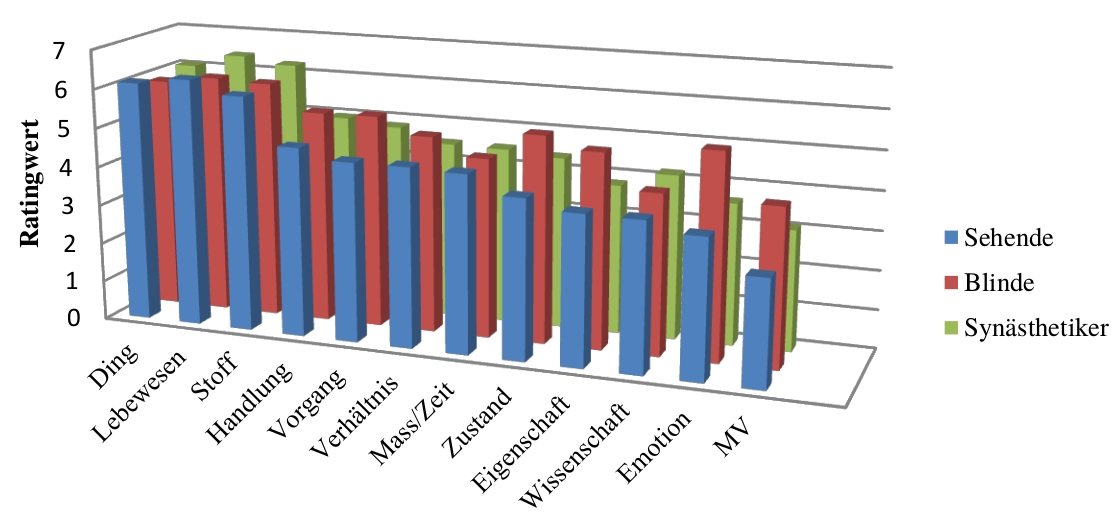
\includegraphics[width=12cm]{images/rating-konkret-abstrakt-schrauf-neu.jpg}
\caption {Ratingwerte für Konkretheit \parencite[][162]{Schrauf2011}}
\label{abb:schrauf-rating}
\end{center}
\end{figure}

Für den emergierenden Artikel ist die Ausweitung von prototypischen Konkreta in Richtung prototypische Abstrakta -- und damit von [+individualisiert] zu [-individualisiert] -- zu erwarten. Eine schrittweise Kombination mit Vertretern der Peripherie kann den Weg für eine graduelle Expansion ebnen. Wegen der Vielschichtigkeit der kognitiven Faktoren, die den Abstraktheitsgrad determinieren, wird an dieser Stelle darauf verzichtet, eine hierarchische Skala innerhalb der \hervor{untypischen} Abstrakta zu modellieren, die eine mögliche Expansionslinie repräsentiert. Alternativ kann man von drei Gruppen ausgehen: den Prototypen (Konkreta und Abstrakta) und einem Übergangsbereich. Wie im nächsten Abschnitt gezeigt wird, ist die potentielle \object{Zählbarkeit} von Abstrakta und Konkreta ein wichtiger Einflussfaktor für Individualität und damit eine zusätzliche Variable, die den Expansionsverlauf des Artikels innerhalb der peripheren Bereiche beeinflusst.  

\subsection{Zählbare Nomen vs. Massennomen}\label{section:mass}

Die bereits angesprochene konzeptuelle \object{Begrenztheit} ist auch zwischen zählbaren und nicht zählbaren Entitäten sowie zwischen Singular- und Pluralformen für Individualitätsunterschiede verantwortlich. Dies zeigen Studien zur sog. \object{count-mass distinction} \parencite[s.][]{Jackendoff1991, Langacker1991, Bisle-Muller1991, Rijkhoff1991,Rijkhoff2002, Corbett2000, Massam2012,Zifonun2012}, die der Frage nach dem konzeptuellen Unterschied von zählbaren Nomen und Massennomen nachgehen. Im Gegensatz zu zählbaren Nomen wie in \REF{ex:count} sind Referenten von Massennomen nicht zählbar und deswegen auch nicht pluralfähig \parencite[77]{Langacker1991}. Sie können sowohl konkret als auch abstrakt sein, verweisen aber stets auf amorphe Referenten mit unscharfen Konturen s. \REF{ex:mass}. 

\begin{exe}
	\ex \label{ex:zaehlbarkeit}
	\begin{xlist}
		\ex \label{ex:count} \object{Buch, Idee}
 		\ex \label{ex:mass} \object{Gold, Vernunft}
 	 	\ex \label{ex:plural} \object{Bücher, Ideen} 
 			\end{xlist}
\end{exe}

\noindent
Langacker subsumiert auch die zählbaren Nomen im Plural (s. \ref{ex:plural}) unter die Massennomen, da diese ebenfalls eine ungebundene Masse repräsentieren \parencite[77]{Langacker1991}. Die Einteilung spiegelt sich auch im grammatischen Verhalten: Beide Substantivklassen können ohne Determinierer eine NP bilden (z.B. \object{Er will Bücher/Gold kaufen}) und lassen Quantifizierer zu, die zählbare Nomen im Singular nicht erlauben (z.B. \object{wenig Bücher/Milch}). Der Unterschied zu den Massennomen liegt darin, dass der Plural eines zählbaren Substantivs auch die einzelnen Bestandteile des Ganzen hervorhebt, vgl. Abbildung \ref{abb:langacker-nomen}.

\begin{figure}[h]
\begin{center}
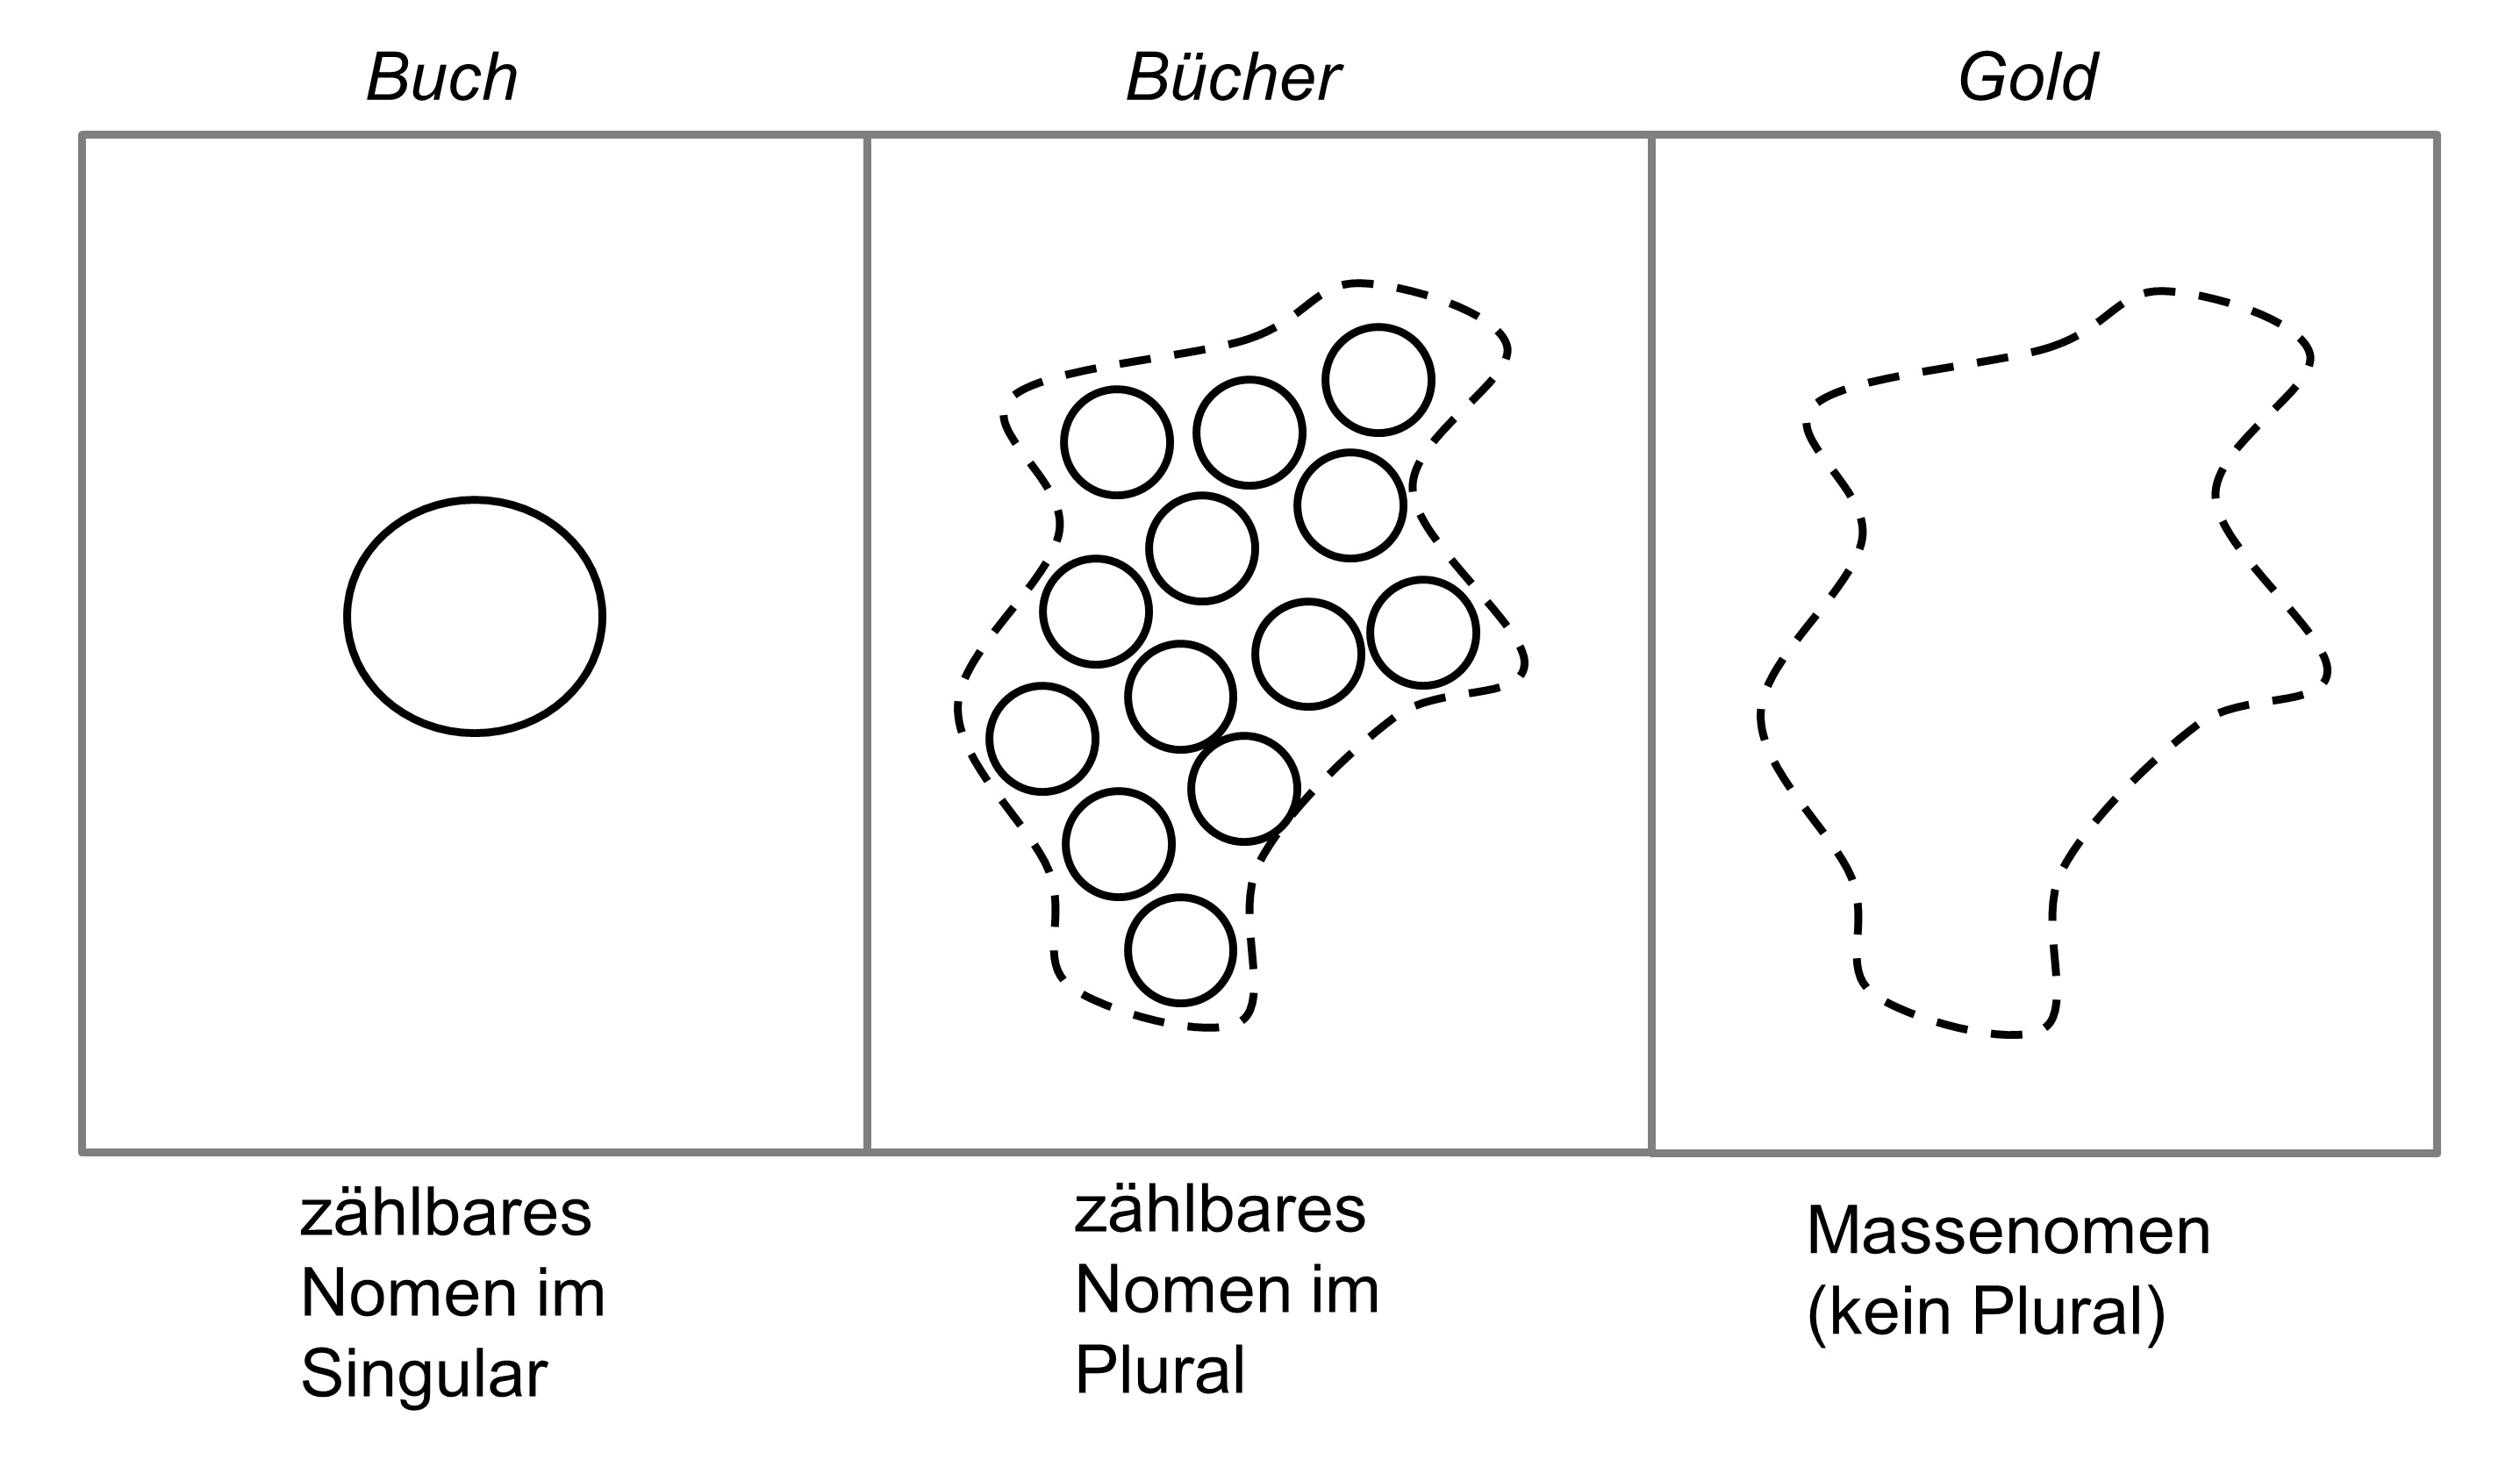
\includegraphics[width=9.5cm]{images/langacker-nomen.jpg}
\caption {Zählbare Nomen und Massennomen im Vergleich \parencite[s.][78]{Langacker1991}}
\label{abb:langacker-nomen}
\end{center}
\end{figure}


Die einzelnen Komponenten bei \object{Bücher} können nur deswegen profiliert werden, weil der Referent nicht aus einer homogenen Masse besteht, sondern eine \object{interne Struktur} \parencite[18]{Jackendoff1991} aus gleichen, distinktiven Einheiten besitzt. Über die Ausprägungen der Variable \object{interne Struktur} in Kombination mit \object{Begrenztheit} lassen sich Substantive nach \textcite[20]{Jackendoff1991} in eine von vier Klassen, s. Tabelle \ref{tab:jack} einordnen. Eine ähnliche Klassifikation nimmt \textcite{Rijkhoff1991,Rijkhoff2002} vor, wenn er von unterschiedlichen \object{Seinsarten} bei Substantiven ausgeht. 
Er unterscheidet \object{Shape} ($\pm$ distinktive Grenzen) und \object{Homogeneity} ($\pm$ agglomerierend) \parencite[s. auch][102-104]{Zifonun2012}.\footnote{In den Sprachen der Welt sind diese Variablen entweder unterschiedlich ausgeprägt oder unterspezifiziert, so dass man sechs Gruppen von Seinsarten annehmen kann; werden diese morphologisch markiert, spricht \textcite[121]{Rijkhoff2002} von \object{Nominalaspekt}.}

\begin{table}
\centering
\begin{tabular}{l>{\itshape}lcc}
\lsptoprule
Substantivklasse & \multicolumn{1}{l}{Beispiel}   & Begrenztheit & Interne Struktur \\ \midrule
Individuum             & Buch       & +                                      & \textminus                                          \\
Kollektivum            & Mannschaft & +                                      & +                                          \\
Agglomerat             & Bücher     & \textminus                                      & +                                          \\
Substanz (=\,Massennomen) &   Gold       & \textminus                                      & \textminus                                          \\\lspbottomrule
\end{tabular}
\caption{Begrenztheit und interne Struktur bei Substantiven \parencite[20]{Jackendoff1991}}
\label{tab:jack}
\end{table}

Wegen ihrer Begrenztheit ist der Individualitätsgrad sowohl bei den Massennomen als auch bei Substantiven im Plural geringer als bei zählbaren Substantiven im Singular. Für Abstrakta wie \object{Idee} kann die Zählbarkeit eine semantische Komponente sein, die einer Determination mit einem emergierenden Artikel förderlich ist, so dass der Expansionspfad innerhalb der Abstrakta vermutlich von \object{zählbar} zu \object{nicht zählbar} (z.B. \object{Finsternis}) verläuft. Kollektiva wie \object{Mannschaft} haben Referenten mit klaren Rändern, allerdings gibt es auch Kollektiva, deren Konturen weniger scharf sind und deren interne Beschaffenheit nicht als Agglomerat von gleichen Individuen konzeptualisiert wird, sondern als Anhäufung einer homogenen Masse, was sie in die Nähe von Massennomen bringt, etwa \object{Laub} oder \object{Vieh} \parencite[s.][120f.]{Zifonun2012}. 
Faktoren wie Größe, Auffälligkeit und Belebtheit hängen sicherlich mit der Einteilung zusammen: Es ist wahrscheinlich, dass \object{Menschen} oder gut sichtbare Objekte wie \object{Berge} als singuläres, begrenztes Kollektiv konzeptualisiert werden (\object{Mannschaft, Gebirge}). Dies unterstützt individualisierte Lesarten. Der kollektive Zusammenschluss der Komponenten von \object{Laub} oder \object{Vieh} lädt hingegen zum nicht-referentiellen und damit nicht-individualisierten Gebrauch ein (\object{Ich muss noch Laub fegen, Der Bauer hat viel Vieh}). Ein Definitartikel kann diese Lesarten zurücknehmen und auch Referenten von Massennomen (\object{das Laub, das Vieh, das Gold}) identifizierbar \hervor{machen}.\footnote{Der umgekehrte Fall ist ebenfalls möglich, nämlich dann, wenn der Kontext ein Massennomen verlangt, aber ein singuläres Nomen verwendet wird, vgl. das makabere Beispiel aus \textcite[81]{Corbett2000}: \object{There was dog all over the road}.} 

Die Substantivklassifikation aus \textcite[104]{Zifonun2012}, die im Rahmen einer Analyse zu Kompositionszweitgliedern als Ausdruck von \object{Nominalaspekt}\footnote{Z.B.\object{-werk} als Marker für Kollektiva, s. \textcite[101]{Zifonun2012}.} modelliert wurde, eignet sich, um  Interaktionen zwischen den genannten Individualitätskriterien zu verdeutlichen. \textcite[103]{Zifonun2012} nimmt zwei Seinsarten für das Deutsche an, die Individuativa (= zählbare Nomen) und die Kontinuativa (= Massennomen), s. \REF{ex:seinsarten} \parencite[basierend auf][]{Rijkhoff1991,Rijkhoff2002}. Orthogonal zu dieser Einteilung verläuft die Opposition konkret-abstrakt sowie die Gruppe der Kollektiva, s. Abbildung \ref{abb:zifonun-seinsarten}.

\begin{exe}
	\ex \label{ex:seinsarten}
	\begin{xlist}
		\ex \label{ex:indi} Individuativum (+Shape, -Homogeneity)
		\ex \label{ex:konti} Kontinuativum (-Shape, +Homogeneity)
 	\end{xlist}
\end{exe}

\begin{figure}
\begin{center}
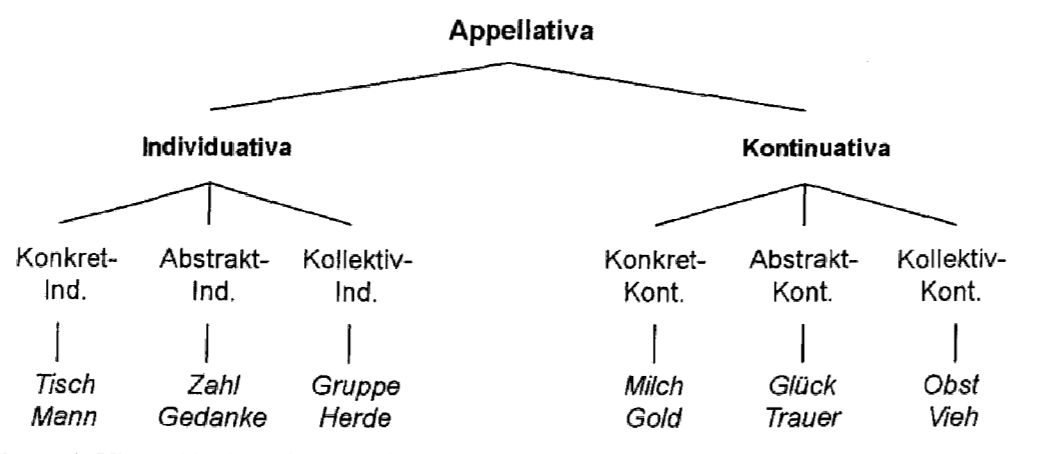
\includegraphics[width=12cm]{images/zifonun-seinarten-neu.jpg}
\caption {Seinsarten im Deutschen aus \textcite[104]{Zifonun2012}\label{abb:zifonun-seinsarten}}
\end{center}
\end{figure}

Die Eigenschaft [+ Shape] sorgt für einen erhöhten Individualitätsgrad bei den Gruppenmitgliedern der Individuativa. Wenn man ein Individualitätsgefälle von Konkreta zu Abstrakta annimmt, dann ist dieses Gefälle Gruppen übergreifend stärker als intern, d.h. \object{Tisch} und \object{Zahl} sind wegen des geteilten Merkmals [+ Shape] konzeptionell ähnlicher als \object{Tisch} im Vergleich zu  \object{Glück}. Es muss angemerkt werden, dass nach \textcite{Rijkhoff2002} ein Nomen wie \object{Gruppe} oder \object{Herde} auf der Anhäufung von Mitgliedern des gleichen Typs beruht, hier z.B. \object {Menschen} oder \object{Tiere}. Die interne Struktur solcher Nomen unterscheidet sich also gegenüber \object{einfachen} Konkreta wie \object{Tisch}. Man müsste also eigentlich das Merkmal [+ Homogeneity] vergeben.\footnote{Vgl. auch die Diskussion oben zum konzeptionell ähnlichem \object{Mannschaft}.} Als Grund, die beiden Substantivtypen dennoch zu gruppieren, nennt \textcite[103]{Zifonun2012}  das gemeinsame grammatische Verhalten: die Fähigkeit zur Pluralbildung und die Kombinierbarkeit mit Kardinalzahlen. Sprachspezifische Kriterien wie diese können nicht ohne Weiteres auf andere Sprachsysteme übertragen werden. Schließlich gibt es Evidenzen, dass Sprachsysteme die Grenze zwischen zählbaren und nicht-zählbaren Referenten an unterschiedlichen Stellen ansetzen: So kennt bspw. das Russische im Gegensatz zum Englischen für \object{Kartoffel} keinen Plural, wohl aber für \object{Frucht} \parencite[80]{Corbett2000}. Es stellt sich dann die Frage \blockcquote[80]{Corbett2000}{how large the component parts of a substance have to be before they are treated as individuals (for speakers of English a pea is large enough, but not for a speaker of Russian}. Interessanterweise betrifft diese Forschungsdiskussion jedoch ausschließlich unbelebte Referenten. Die Einteilung von Individuativnomen mit dem Merkmal [+belebt] kann deswegen auch sprachübergreifend als eigene höchst individualisierte Klasse gerechtfertigt werden. Schlägt sich die konzeptuelle Zuordnung eines Objekts in die Kategorie \object{zählbar} auch in der Grammatik nieder, so ist dies ein zusätzlicher Hinweis auf eine erhöhte Individualität und ein Faktor, der die Determination mit Artikelwort begünstigt. 

\section{Belebtheit in Interaktion mit anderen Faktoren} \label{sec:andere-kog}
 
Im vorhergehenden Abschnitt wurde gezeigt, wie Belebtheit und Individualität zusammenhängen. Nachfolgend werden zwei weitere Faktoren besprochen, die ebenfalls mit der Belebtheit interagieren und damit einen Einfluss auf die Artikelsetzung haben. In Abschnitt \ref{sec:partizipanten} wird auf semantische Rollen und ihre prototypische Besetzung eingegangen. In Abschnitt \ref{sec:relevanz} steht der Faktor Relevanz im Mittelpunkt.
 
\subsection{Semantische Rollen}\label{sec:partizipanten}

Ein hoher Belebtheitsgrad korreliert mit bestimmten semantischen Rollen\footnote{Auch: \hervor{Partizipantenrollen} \parencite[vgl.][]{Lehmann2004a}.} \parencite[vgl. u.a.][]{Hopper1980,Comrie1989,Yamamoto2006}. So wird die Agensrolle typischerweise mit einem Referenten besetzt, der eine Handlung willentlich ausführt oder sogar verursacht, s. Beispiele \REF{ex:agens}.

\begin{exe}
	\ex \label{ex:agens}
	\begin{xlist}
		\ex \label{ex:voll} \textbf{Paul} ignoriert den Kommentar. 
 		\ex \label{ex:verursacher} \textbf{Moritz} öffnet die Tür.
	\end{xlist}
\end{exe}

\noindent 
Belebte und insbesondere menschliche Referenten bringen die notwendigen ontologischen Eigenschaften mit, um Handlungen zu planen,  auszuführen und die Kontrolle (über ein Patiens) zu ergreifen. Traditionell wird Belebtheit sogar als definitorisch für die Agensrolle angesehen \parencite[16]{Primus2012}. 
Doch auch unbelebte Referenten sind fähig, Handlungen auszuführen, man denke etwa an die  Kommunikation zwischen Mensch und Maschine \parencite[s. weiterführend][18]{Primus2012}. Am mehrdimensionalen Proto-Agens-Konzept, das von \parencite{Dowty1991} in die Forschungsdiskussion eingeführt und seither breit rezipiert wurde \parencite[vgl. u.a.][]{Ackermann2001,Primus2012,Szczepaniak2016}, wird besonders gut deutlich, dass das Merkmal Belebtheit für einen Referenten nicht konstitutiv ist, um die Agensrolle zu erfüllen. Es vereint sowohl die oben beschriebene prototypische Agensrolle, als auch agens"-ähnliche Partizipanten. Nachfolgend sind die wichtigsten Dimensionen aufgeführt, die dem Proto-Agens zugesprochen werden  (basierend auf \cite[][572f.]{Dowty1991};   \cite[25]{Primus2012}).  

\begin{description}
\item[Volitionalität:] \object{\textbf{Er} hört dem Vortrag zu.}
\item[Empfindung (Wahrnehmung):] \object{\textbf{Sie} mag Comics.}  
\item[Verursachung:] \object{\textbf{Er} zerstört den Tisch./ \textbf{Rauchen} verursacht Krebs.}  
\item[Selbstinduzierte Bewegung:] \object{\textbf{Sie} fiel./ \textbf{Wasser} floss ins Boot.} 
\item[Besitz:] \object{\textbf{Sie} besitzt einige Häuser.}
\end{description}

Wie \textcite[][151f.]{Yamamoto1999} hervorhebt, entspringen Belebtheit und semantische Rollen nicht der gleichen kategorialen Ebene: Der Belebtheitsgrad bezieht sich immer auf einen dem Referenten inhärenten Status. Es ist eine ontologisch begründete Klassifikation. Semantische Rollen sind hingegen relationale Begriffe, die vom Situationstyp determiniert werden, den das Verb denotiert \parencite[13]{Lehmann2004a}. Ihre Besetzung ist prinzipiell variabel: Ein belebter Referent wie \object{Moritz} kann bspw. sowohl als Agens als auch als Patiens auftreten, d.h. als der von der Handlung maximal Betroffene, s. Beispiel \REF{ex:rollen}. 
 
\begin{exe}
	\ex \label{ex:rollen}
	\begin{xlist}
	 	\ex \object{Moritz} (= Agens) \object{gibt Paul ein Buch.}
		\ex \object{Paul kitzelt Moritz} (= Patiens).
 
	\end{xlist}
\end{exe}
\noindent
 
Wird ein unbelebter Referent personifiziert, verändert sich nicht sein Belebtheitsgrad, sondern seine semantische Rolle und mit ihr die Art, wie  der Referent konzeptualisiert wird (\object{Die Hoffnung spricht}). 

\textcite[12]{Lehmann2004a} zufolge können belebte Referenten das größte Spektrum an semantischen Rollen einnehmen. Neben Agens und Patiens sind dies Experiens, Komitativ, Emittent, Rezipient, Synpatheticus und Benefiziär.  Für Referenten, die weiter unten auf der Belebtheitsskala\footnote{\textcite{Lehmann2004a} sprechen nicht von Belebheits- sondern von einer 
Empathiehierarchie, vgl. auch Abschnitt \ref{sec:belebt}.} angesiedelt sind, ist die Rollenauswahl begrenzt, doch gibt es auch hier prototypische Besetzungen. So fungieren unbelebte Referenten typischerweise als Instrument bzw. \herkur{Force} oder sie geben temporale oder lokale Relationen an \parencite[76]{Primus2012}. Letztere können auch von belebten Referenten ausgefüllt werden (etwa: \object{Ich gehe zum Arzt} = Ziel). 

Definitorisch für die semantischen Rollen ist die Nähe zum Situationskern, welche im Parameter Involviertheit bzw. Zentralität zum Ausdruck kommt \parencite[6]{Lehmann2004a}. Bei einer dynamischen Transitivsituation sind bspw. Agens und Patiens maximal involviert, weil sie konstitutiv und charakteristisch für die Handlung sind. Das Gleiche gilt für die Rolle des Rezipienten bei einer Transfersituation. Weniger zentral sind fakultative Rollen, die prinzipiell zu jeder Situation hinzutreten können, um diese zu modifizieren, d.h. u.a. temporale, lokale und kausale Rollen. Sie kommen  meist als Adverbiale vor.

Es ist zu erwarten, dass der emergierende Definitartikel in seiner Funktion als Individualisierer (s. Abschnitt \ref{sec:individualisierer}) bzw. Marker von Diskursprominenz (s. Abschnitt \ref{sec:kata}) zuerst bei zentralen semantischen Rollen erscheint und erst später in die \hervor{Handlungsperipherie} eindringt. Die Beobachtungen von \textcite{Himmelmann1998} stützen diese Hypothese: So sind es vor allen Dingen die \hervor{adpositional expressions} und damit meist Adverbiale, die in vielen Sprachen keinen Definitartikel aufweisen. Im Gegensatz zu zentralen Partizipanten denotieren sie typischerweise Referenten, die einen niedrigen Referentialitätsgrad haben, etwa \object{im Sommer, in Wirklichkeit, auf Erden}.  Sie dienen dazu, das Setting, in dem die Partizipanten agieren, genauer zu bestimmen \parencite["-="- orientierende Funktion, s.][118]{Himmelmann1997} und werden daher selten als Diskurstopik wiederaufgenommen. Eine besondere sprachliche Hervorhebung ist in diesen Fällen also nicht notwendig. Wahrscheinlich sorgt die zunehmende Obligatorisierung in anderen syntaktischen Kontexten dafür, dass der Definitartikel auch die weniger zentralen Partizipanten analogisch erfasst, sofern sich die artikellose Phrase noch nicht zu sehr kognitiv eingeschliffen hat (zu diesem \object{Entrenchment}-Prinzip vgl. ausführlich Abschnitt \ref{sec:entrenchment}). 

\subsection{Relevanz}\label{sec:relevanz}

Die Konzeptualisierung von Objekten hängt auch mit dem Faktor Relevanz zusammen \parencite[s.][347]{Szczepaniak2011}.  
Dieser korreliert einerseits mit der Belebtheit: Belebte Referenten sind relevanter als unbelebte, da sie  über eine höhere Handlungsgewalt verfügen und damit das Potential besitzen, das Denken, Handeln und Leben des Sprechers zu beeinflussen. Anderseits ist die Relevanz eine eigenständige Variable, deren Ausprägungen kulturell-gesellschaftlich definiert ist. Vor dem Hintergrund mittelalterlicher Hierarchiegefüge ist der König bspw. relevanter als seine Bediensteten, der Mann ist relevanter als die Frau. Im christlichen Kulturkreis genießt Gott und damit eine übermenschliche Entität, die höchste kulturelle Relevanz. Auch Gegenstände können für Sprecherinnen und Sprecher eine erhöhte Relevanz haben, z.B. die Bibel oder ein bestimmtes Lied. Und für Menschen in Kriegsgebieten hat das Abstraktum \object{Friede} sicher eine höhere Relevanz als für Menschen in friedlichen Regionen.  Darüber hinaus existiert oft auch eine textuelle Relevanz  \parencite[347]{Szczepaniak2011}: Sie gilt, wenn ein Referent besonderes eng mit dem Textthema verbunden ist oder eine zentrale Rolle für den Ausgang einer Geschichte oder die Argumentationsführung einnimmt.

Die Wirkung von Relevanz wird bei der Entwicklung der satzinternen Großschreibung sichtbar: Im frühen 17. Jahrhundert ist die Majuskelsetzung pragmatisch gesteuert und dient u.a. dazu, religiöse Verehrung (Großschreibung von Nomina sacra) oder soziale Ehrerbietung  (Großschreibung von Titeln oder Standes- und Amtsbezeichnungen) zu markieren \parencite[73]{Bergmann1999}. Ein Beispiel für den Einfluss der textuellen Relevanz ist die konsequente Großschreibung von  <Kasten> als Synonym für die Arche Noah in der Luther-Bibel von 1534 \parencite[352]{Szczepaniak2011}. In diesem Text dominiert ansonsten die Kleinschreibung.

Auch für die Entwicklung des Definitartikels lässt sich postulieren: Umso höher der Relevanzgrad, umso wahrscheinlicher ist es, dass der emergierende Definitartikel gesetzt wird. Belebte und kulturell wichtige Referenten sind von sich aus weit oben auf der Relevanzsskala angesiedelt, so dass bei ihnen eine frühe Hervorhebung zu erwarten ist. 
Doch das Relevanzprinzip kann auch bei anderen Referenten greifen. So zeigt \textcite[]{Epstein1993,Epstein1994} an altfranzösischen Sprachdaten, dass der sich entwickelnde Artikel pragmatisch genutzt wird, um bspw. Abstrakta, die gewöhnlich als unspezifische Entitäten konzeptualisiert werden und dann undeterminiert bleiben, in bestimmten Fällen eine eindeutig identifizierbare und diskursprominente Lesart zuzuschreiben. Dies ist in einer der frühesten Überlieferung  (\hervor{La chanson de Roland} um 1080) zu sehen, wenn von dem Tod (\object{la mort}) oder dem Verrat (\object{la traïsun}) einer der Leserschaft bekannten Person berichtet wird \parencite[71f.]{Epstein1994}. Eine ähnliche pragmatisch gesteuerte Artikelsetzung vermutet auch \textcite[218]{Oubouzar1989} für das frühe Althochdeutsche. 

\section{Zusammenfassung} \label{sec:bel-zusammenfassung}

Aus den bisherigen diachronen Untersuchungen lässt sich die Hypothese ableiten, dass die kognitiv-linguistische Kategorie Belebtheit den Expansionsweg des ermergierenden Definitartikels lenkt. Der Startpunkt ist bei den belebten und insbesondere menschliche Referenten zu suchen, da Sprecherinnen und Sprecher diesen meist die höchste Relevanz im Diskurs zuschreiben.
Sie sind kognitiv besonders auffällig, da sie typischerweise den größten Handlungsraum im Diskurs einnehmen. Das ursprünglich demonstrative \object{dër} kann diese Diskursprominenz sprachlich unterstreichen. Da jede Form des Determinierens einen kognitiven Abgrenzungsprozess beinhaltet -- aus einer Menge von möglichen Referenten wird eine Teilmenge ausgewählt, wodurch andere in Frage kommende Referenten ausgegrenzt werden -- ist zu erwarten, dass Referenten mit unscharfen Grenzen, darunter Abstrakta, Kollektiva und Stoffe sowie zählbare Nomen im Plural, \hervor{schlechtere} Kandidaten für eine definite Kennzeichnung sind als Referenten mit scharfen Grenzen. Zu diesen gehören konkrete, zählbare, singulare Entitäten. Sie sind empirisch direkt wahrnehmbar, haben einen höheren Kontrast zu ihrer Umwelt und zu anderen Referenten als konturlose Objekte und sind dadurch stärker individualisiert. 

Mit zunehmender Konventionalisierung -- so die Hypothese -- verliert \object{dër} seine pragmatische Kraft und wird zum obligatorischen Marker für alle Substantivklassen. Neben der Individualität korreliert mit einem hohen Belebtheitsgrad auch der Faktor Agentivität, weswegen dieser Faktor in das Belebtheitsmodell, das der nachfolgenden Untersuchung zugrunde liegt, mit einbezogen wird, vgl. Abbildung \ref{abb:belebtheit-gesamt}, die auf den Darstellungen von \textcite[345]{Szczepaniak2011} und \textcite[98]{Nubling2012} basiert.  
    
\begin{figure}[h]
\begin{center}
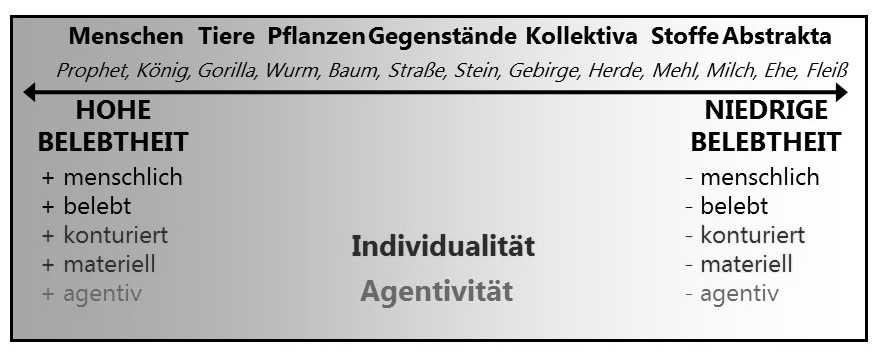
\includegraphics[width=10cm]{images/belebtheits-skala-neu-sw.jpg}
\caption{Belebtheit und korrelierende Faktoren}
\label{abb:belebtheit-gesamt}
\end{center}
\end{figure}


Nicht mit in der Darstellung aufgenommen ist die Zählbarkeit und damit zusammenhängend der Numerus eines Objekts. Diese Kriterien laufen quer zur Belebtheitshierchie, in dem Sinne, dass im Prinzip alle konkreten Entitäten (also Menschen, Tiere, Gegenstände) je nach Vorkommen und Konzeptualisierung in ihrer Zählbarkeit und damit im Numerus variieren. Für Abstrakta ist die Unterscheidung nicht relevant. Denn selbst zählbare Abstrakta wie \object{Grausamkeit} weisen keine numerusspezifischen konzeptuellen Unterschiede auf, welche die Individualität beeinflussen würden. Generische Lesarten sind bei allen Referenten prinzipiell möglich, bei Referenten auf der rechten Seite des Modells allerdings wahrscheinlicher als auf der linken, so dass dies einer frühen Determinierung mit \object{dër} zusätzlich im Wege steht. Eine hohe gesellschaftlich-kulturelle und textuelle Relevanz ist bei belebten Referenten zwar besonders wahrscheinlich. Je nach Kontext und Textthema ist Relevanz aber auch ein Faktor, der bei unbelebten und abstrakten Referenten wirksam sein kann, so dass er orthogonal zur linearen Hierarchie verläuft. 

%\chapter{Untersuchungsmethode}\label{methode}

Wie in den vorhergehenden theoretischen Abschnitten der Arbeit dargelegt wurde, ist es das Ziel der vorliegenden Untersuchung, eine systematische Analyse der ahd. Struktur [\object{dër}\,+\,N] nach  kognitiv-linguistischen, funktionalen und formalen Kriterien durchzuführen. Das vorliegende Kapitel legt die Untersuchungsmethode und die Vorgehensweise offen. Nachdem in Abschnitt \ref{sec:ahd} die Sprachstufe Althochdeutsch und Möglichkeiten ihrer korpuslinguistischen \is{Korpuslinguistik}  Erschließung ausgelotet werden, erfolgt in Abschnitt \ref{sec:textauswahl} ein Überblick über die Texte, die als Basis für die Untersuchung dienen. Gegenstand von Abschnitt \ref{sec:datenaufbereitung} sind die Schritte der Datenaufbereitung, welche eine genaue Beschreibung des Vorgehens bei der \isi{Annotation} und eine Beschreibung der Annotationsebenen \is{Annotation} einschließen. In Abschnitt \ref{sec:analysemethoden} wird das Zusammenspiel von qualitativen und quantitativen Analysemethoden diskutiert sowie der Umgang mit Differenzbelegen \is{Differenzbeleg} erläutert. Das Kapitel schließt mit einer zusammenfassenden Übersicht. 

\section{Das Althochdeutsche und seine korpuslinguistische Erschließung}\label{sec:ahd}\largerpage

Aus der althochdeutschen Sprachperiode (750--1050) liegen uns nur relativ wenige, zufällig überlieferte und teilweise fragmentarische Textdenkmäler vor \parencite[zur Überlieferungsproblematik s. ausführlich][49--105]{Sonderegger2003}.\footnote{Fleischer bemerkt über die ahd. Quellenlage: \blockcquote[27]{Fleischer2006}{In rein quantitativer Hinsicht ist die Überlieferung des Althochdeutschen innerhalb der altgermanischen Sprachen weder besonders groß (beispielsweise im Vergleich zum Altnordischen oder Altenglischen) noch besonders  klein (beispielsweise im Vergleich mit dem Altniederdeutschen}. Gemessen an heutigen Maßstäben ist die Überlieferungsgröße mit weit unter einer Million Textwörter (s. Abschnitt \ref{sec:ddd}) natürlich als klein einzustufen -- zum Vergleich: das Deutsche Referenzkorpus \is{Korpus} (DeReKo) beläuft sich auf knapp 47 Milliarden Textwörter (Stand 18.01.2020), s. \url{http://www1.ids-mannheim.de/kl/projekte/korpora.html}.} Man muss sich bei der Arbeit mit althochdeutschem Sprachmaterial daher immer bewusst sein, dass  nur ein sehr kleiner Ausschnitt der damaligen Sprachwirklichkeit abgebildet wird, der darüber hinaus mindestens durch regionale und textsortenspezifische Eigenheiten verzerrt ist  \parencite[27--31]{Fleischer2006}. Aus diesen Gründen können generelle Aussagen über das Althochdeutsche nur mit Vorbehalt gemacht werden. 

Die Fragestellung der vorliegenden Arbeit, ob \object{dër} als Demonstrativ- \is{Demonstrativartikel} oder Definitartikel \is{Definitartikel} zu klassifizieren ist, setzt eine Analyse des textuellen Kontextes voraus. Zudem wurde in Abschnitt \ref{sec:schema} gezeigt, dass die Entwicklung von \object{dër} auch von systemischen Veränderungen auf Phrasenebene \is{Phrase} abhängig ist. Ein \isi{Korpus} des Althochdeutschen, das für solche syntaktischen Fragestellungen angemessen wäre, sollte daher einerseits längere und kohärent zusammenhängende Textabschnitte enthalten. Andererseits muss es hinsichtlich der Variablen Zeit, Region und Textsorte ausbalanciert\footnote{Zum Begriff des \object{balanced corpus}, vgl. \cite[6]{Atkins1992}.} sein, da diese die Ausprägung syntaktischer Strukturen \is{Nominalsyntax} beeinflussen \parencite[74]{Fleischer2011}.\footnote{So zeigt beispielsweise \textcite[47]{Eggenberger1961}, wie metrische \is{Metrik} Zwänge die Setzung von Subjektpronomina \is{Subjekt}\is{Personalpronomen}im ahd. Otfrid steuern.} Aufgrund der bruchstückhaften Überlieferungssituation ist ein solcher Korpusaufbau \is{Korpus} allerdings nicht zu bewerkstelligen. So weist bspw. ein nach Ort und Zeit strukturiertes \isi{Korpus} des 9. Jahrhunderts, wie \textcite{Fleischer2011} demonstrieren, zahlreiche Lücken auf,  s. Tabelle~\ref{tab:9Jh-matrix}. Auch für die vorhergehenden und nachfolgenden Jahrhunderte gibt es nur fragmentarische Überlieferungen.

\begin{table}
\resizebox{\textwidth}{!}{\begin{tabular}{ccccccccc}
\lsptoprule
  & \multicolumn{2}{c}{Ostfränk.} & \multicolumn{2}{c}{Südrheinfr.} & \multicolumn{2}{c}{Aleman.} & \multicolumn{2}{c}{Bair.} \\
  \cmidrule(lr){2-3}\cmidrule(lr){4-5}\cmidrule(lr){6-7}\cmidrule(lr){8-9}
        & Prosa         & Poesie        & Prosa         & Poesie         & Prosa        & Poesie       & Prosa       & Poesie      \\ \midrule
800--850 & T        & \textminus             & \textminus             & \textminus              & \textminus            & \textminus            & MF         & \textminus           \\
850--899 & \textminus             & \textminus             & \textminus             & O         & \textminus            & \textminus            & \textminus           & \textminus           \\ \lspbottomrule
\end{tabular}}
\caption{Strukturiertes \isi{Korpus} des 9. Jh. \parencite[75]{Fleischer2011} (T = Tatian, O = Otfrid, MF = Monseer Fragmente)\label{tab:9Jh-matrix}}
\end{table}  

Auch wenn die Quellenlage den Aufbau eines balancierten \isi{Korpus} nicht zulässt, kann man sich die methodischen Errungenschaften der modernen \isi{Korpuslinguistik} zunutze machen. Dies bedeutet, dass der Analyse eine systematische Auswahl von Belegen zugrunde liegen sollte: Das Ziel historischer Korpusuntersuchungen \is{Korpuslinguistik} muss sein, die vorhandenen Quellen nicht bloß -- wie es \textcite[1310]{Wegera2000} ausdrückt -- \hervor{"`steinbruchartig"' aus[zu]schlachten}, sondern gesamtheitlich zu analysieren.\footnote{\textcite{Wegera2000} bezieht sich hierbei in erster Linie auf mittelhochdeutsche Quellen. Die Aussage lässt sich jedoch ohne Weiteres auf das Althochdeutsche übertragen.} \textcite[382]{Fleischer2015} präzisiert den damit verbundenen methodischen Paradigmenwechsel:
"`An die Stelle mehr oder minder zufällig zusammengestellter Belege tritt die konsequente und exhaustive Auswertung bestimmter Text(ausschnitt)e in Bezug auf die zu untersuchenden Phänomene"'. Eine solche Arbeitsweise wirkt der Versuchung entgegen, theoretische Entwürfe lediglich auf Basis ausgewählter (und damit oft hypothesenkonformer) Einzelbelege zu modellieren. Zudem schützt sie davor, auffälligen -- weil von der modernen Sprache abweichenden -- Strukturen einen Stellenwert im älteren Sprachsystem einzuräumen, der durch die tatsächliche Vorkommenshäufigkeit vielleicht gar nicht gerechtfertigt werden kann \parencite[383]{Fleischer2015}. Darüber hinaus müssen die für die Untersuchung zentralen linguistischen Kategorien operationalisiert \is{Operationalisierung} werden  \parencite[113--116]{Lemnitzer2015}. Denn, damit die Klassifizierung eines sprachlichen Ausdrucks nicht das Ergebnis der individuellen Interpretation bleibt, ist es wichtig, möglichst objektive \is{Operationalisierung} Kriterien zu entwickeln und diese, z.B. in Form von \isi{Annotationsrichtlinien}, offenzulegen. Die Qualität solcher Richtlinien kann u.a. über sog. \herkur{Inter Annotator Agreements} gewährleistet \is{Annotation} werden.\footnote{Vgl. hierzu für die vorliegende Arbeit Abschnitt \ref{sec:annotationsschritte}.} 

Wie diese methodischen Anforderungen, also a) die exhaustive Auswertung von längeren ausgewählten Texten/Textausschnitten und b) die \isi{Operationalisierung} der für die Fragestellung relevanten Kategorien, bei der Untersuchung zum Entwicklung des Definitartikels \is{Definitartikel} umgesetzt wurden, dokumentieren die nachfolgenden Abschnitte.


\section{Textauswahl}\label{sec:textauswahl}

Für die Untersuchung wurden die fünf längsten Texte aus der ahd. Sprachperiode ausgewählt: Isidor von Sevilla (I), Monseer Matthäus (M), Tatians Evangelienharmonie (T), Otfrids Evangelienbuch (O) und Notkers Boethius (Buch 1,2) (N), s. Tabelle~\ref{tab:ddd-auswahl}. Die Zusammenstellung ähnelt Oubouzars Datengrundlage \parencite[41--42]{Oubouzar1989}, allerdings mit dem Unterschied, dass die Auswahl um das Matthäus Evangelium aus den Monseer Fragmenten erweitert wurde und Tatians sowie Otfrids Evangelienbuch in ihrer Gesamtheit\footnote{Oubouzars \isi{Korpus} enthält Kapitel 1--75 aus dem Tatian und Kapitel 2 und 3 aus Otfrids Evangelienbuch.} betrachtet werden.  Die Eigenheiten der einzelnen Texte werden in den nachfolgenden Abschnitten (\ref{sec:isidor}--\ref{sec:notker}) vorgestellt.\largerpage[2]

\begin{table}[p]
\begin{tabular}{llrc}
\lsptoprule
Text                  & Textsorte      & Ahd. Textwörter & Entstehung \\ \midrule
I                      & Prosa (lat.-ahd.)          &   4.980                  & um 790       \\
M         & Prosa (lat.-ahd.)          & 4.604            & um 810              \\
T & Prosa (lat.-ahd.)          & 37.481                  & um 840              \\
O     & Ahd. Versdichtung          & 60.615               & um 870              \\
N   & Prosa (lat.-ahd. Mischtext) &  17.463               & um 1025             \\ \lspbottomrule
\end{tabular}
\caption{Textauswahl für die Untersuchung}
\label{tab:ddd-auswahl}
\end{table}

\begin{figure}[p]
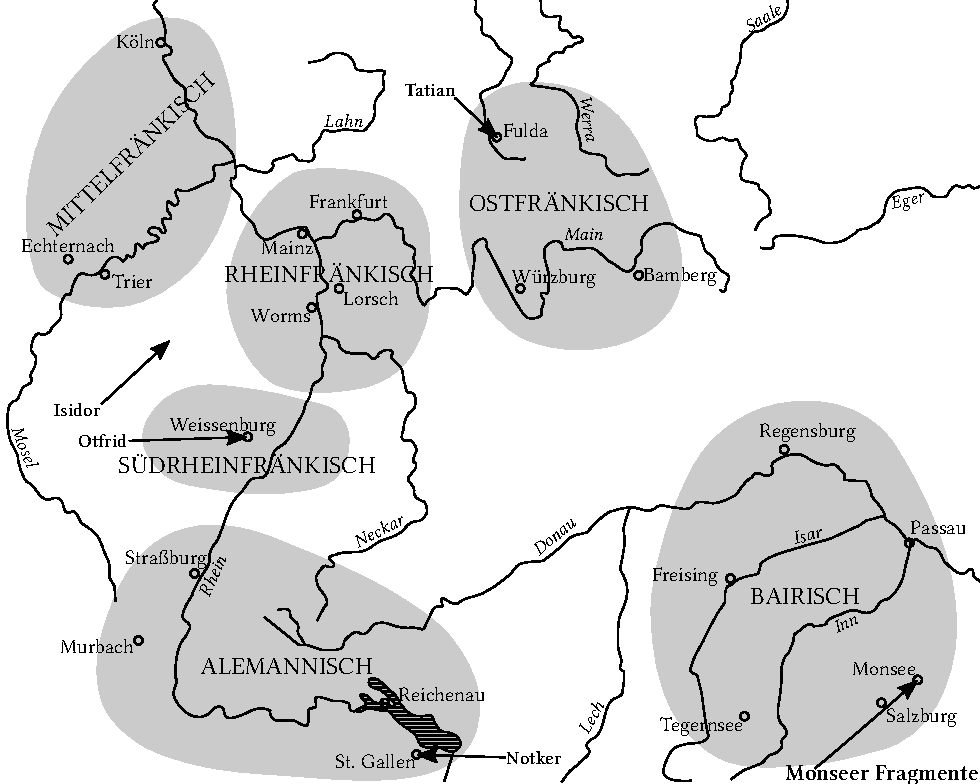
\includegraphics[width=\textwidth]{images/koenig-atlas.pdf}
\caption {Herkunft der ausgewählten Texte; erweiterte Grafik auf Basis von  \textcite[66]{Konig2015}\label{abb:schreiborte}}
\end{figure}

Das zeitliche Nacheinander der Texte suggeriert ein gewisses Maß an diachroner Kontinuität. Dennoch muss man mit Aussagen über mögliche Entwicklungslinien  vorsichtig sein \parencite[vgl. hierzu auch][158]{Leiss2000}, da die Texte auch eine diatopische Varianz aufweisen, s. Abbildung~\ref{abb:schreiborte}. Insbesondere bei den zeitlich enger beieinander liegenden Texten (Isidor, Monseer Fragmente und bei Tatian) ist daher auch von regional bedingten Einflüssen auszugehen. Der Unterschied von rund 200 Jahren zwischen der Isidorübersetzung und Notkers Boethius ist hingegen groß genug, um diachrone Veränderungen abzubilden.


Doch selbst wenn man die Texte lediglich als isolierte \hervor{Sprachinseln} innerhalb eines spezifischen Zeit-Raum-Koordinatensystems \parencite[157]{Leiss2000} betrachtet, so ist es doch immerhin möglich den jeweiligen Entwicklungsstand eines sprachlichen Ausdrucks (hier: [\object{dër}\,+\,N]) pro Text
zu konstatieren \parencite[vgl. zu diesem Vorgehen auch][29]{Himmelmann1997}. Denn anders als in typologisch-synchronen Untersuchungen, bei denen der zukünftige Entwicklungspfad eines Sprachzeichens nie mit Gewissheit vorhergesagt werden kann, weiß man bei einer historisch-diachronen Untersuchung zumindest, zu welchem  Sprachzeichen sich ein bestimmtes Element entwickelt. Daher sind retrospektiv auch Zwischenstadien in der Entwicklung auszumachen.      


\subsection{Isidor} \label{sec:isidor}

Bei der  ahd. Isidor-Übersetzung (meist verkürzt bezeichnet als \hervor{ahd. Isidor} oder einfach \hervor{Isidor}\footnote{Eine andere Bezeichnung ist \hervor{Pariser Isidor}, gemäß des Aufbewahrungsortes -- die Pariser Nationalbibliothek.}) handelt es sich um eine Übersetzung eines theologischen Traktats des Bischofs Isidor von Sevilla (um 560--636) mit dem Titel \herkur{De fide catholica ex veteri et novo testamento contra Iudaeos}. Sie ist kulturgeschichtlich in die sprachpolitische Missionierungsarbeit Karls des Großen einzuordnen \parencite[vgl.][36--38]{Schlachter2012}. Nach \textcite[VIII][]{Eggers1964} kann das Schriftstück auf Ende des 8. Jahrhunderts datiert werden; die sprachlichen Merkmale deuten auf das Westrheinfränkische hin \parencite{Matzel1970}.\footnote{Für eine intensive philologische Diskussion des ahd. Isidors und der Monseer Fragmente als Teil der sog. Isidor-Gruppe (auch im Vergleich zum ahd. Tatian) sei auf \textcite[17--53]{Schlachter2012} verwiesen.} 

In den insgesamt neun Kapiteln des Isidors steht die lateinische Vorlage dem ahd. Text pa"-ral"-lel innerhalb einer Textseite gegenüber, vgl. Abbildung~\ref{abb:isidor4}.\footnote{Cod. Paris. (Bibl. Nat., Ms. lat.) 2326, p. 2v; 
\url{https://gallica.bnf.fr/ark:/12148/btv1b84260348/f16}; zuletzt aufgerufen am 12.02.2020.} Der Beginn des Traktats ist nur in Bruchstücken als Teil der Monseer Fragmente (s. Abschnitt \ref{sec:monsee}) überliefert; zudem fehlen große Textteile, die vermutlich dem 9. Kapitel folgten \parencite[25]{Schlachter2012}.

\begin{figure}[h]
\begin{center}
  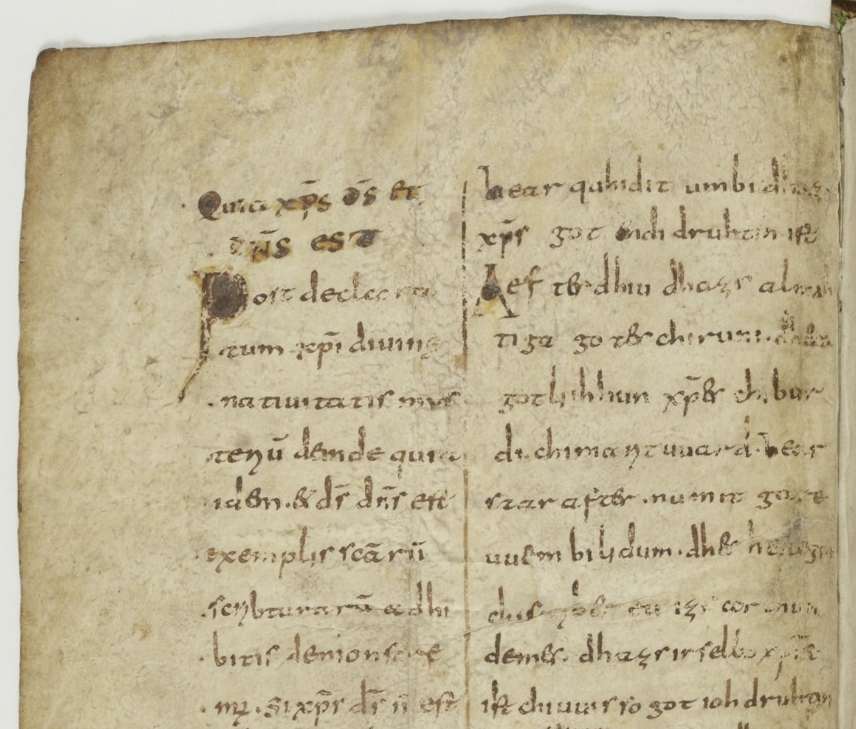
\includegraphics[width=10 cm]{images/isidor-kap-3-ausschnitt.jpg}
  \caption {Der Anfang des 3. Kapitels des ahd. Isidor}
\label{abb:isidor4}
\end{center}
\end{figure} 

%In schwarz-weiß: images/isidor-kap-3-ausschnitt-sw.jpg

Nach \textcite{Matzel1970} wechseln im Schriftstück zwei Übersetzungsstrategien einander ab: Während übersetzte Bibelzitate dem lateinischen Vorbild stark ähneln, werden die auf diesen Zitaten aufbauenden, argumentativen Teile -- zugunsten der \blockcquote[357]{Matzel1970}{theologischen Beweisführung} -- nicht wortwörtlich, sondern meist nur sinngemäß wiedergegeben. Einflüsse der lateinischen Vorlage sind daher vor allem bei den Bibelzitaten zu erwarten \parencites()()[33]{Fleischer2006}[45--46]{Schlachter2012}. Weil der Text sich durch ein stetes Vor- und Zurückverweisen zwischen Bibelstelle und argumentativen Passagen ausweist, ist außerdem damit zu rechnen, dass dem genuinen \isi{Demonstrativum} \object{dër} als kohärenzstiftendes Mittel eine besondere Rolle zukommt. So zeigt sich bereits in einer Pilotstudie zum 4. Kapitel \parencite[]{Szczepaniak2015}, dass \object{dër} sehr häufig für den anaphorischen \is{anaphorisch} Bezug zu abstrakten \is{Abstraktum}  biblischen Konzepten, etwa \object{drinissa} (\extrans{Dreifaltigkeit}), gebraucht wird. Damit unterscheidet sich Isidor von primär narrativen Textsorten wie den Monseer Fragmenten oder dem größten Teil des ahd. Tatian.   


\subsection{Monseer Matthäus} \label{sec:monsee}

Der Monseer Matthäus ist Teil der Monseer Fragmente. Dabei handelt es sich um eine Sammlung von Einzeltexten, die um 810 im Kloster Mondsee (Nahe Salzburg) ins Bairische übertragen wurden. Überliefert sind Ausschnitte aus den folgenden fünf Texten \parencite{Krotz2003}.


\begin{itemize}
\item Teile von Isidors \herkur{De fide catholica ex veteri et novo testamento contra Iudaeos} 
\item das Matthäus-Evangelium
\item die Predigt \herkur{De vocatione gentium}
\item der Schluss einer unbekannten Predigt
\item die Predigt Nr. 76 des Augustus
\end{itemize}

Den Monseer Fragmenten als Teil der sog. Isidor-Gruppe wird eine hohe Übersetzungsqualität zugeschrieben. Es sind die \blockcquote[129]{Sonderegger2003}{früheste[n] Denkmäler einer selbstständigen althochdeutschen Übersetzungsprosa von erstaunlicher Sprachbeherrschung in der Genauigkeit und Übertragung wie in der eigenen Gestaltung}. 
Leider sind die überlieferten Ausschnitte textlich nicht homogen, was die Vergleichbarkeit untereinander sowie zu anderen Texten einschränkt. Auch in der Überlieferungsqualität sowie der Länge gibt es starke Unterschiede \parencite[s. ausführlich][]{Krotz2002,Krotz2003}. Quantitativ bildet das Matthäus-Evangelium, das mit ca. 120 ahd.-lat. Parallelversen zu knapp zwei Dritteln überliefert ist, das Kernstück der Monseer Fragmente 
\parencites()()[82]{Matzel1970}[26--27]{Schlachter2012}.
Abbildung~\ref{abb:MF-handschrift} zeigt einen Ausschnitt.\footnote{Hannover, Landesbibliothek; \url{https://de.wikipedia.org/wiki/Datei:Mondseer-fragment-3.png}; zuletzt aufgerufen am 12.02.2020.} 

\begin{figure}[h]
\begin{center}
  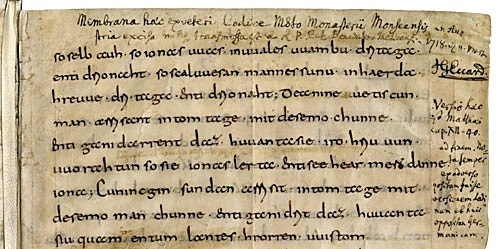
\includegraphics[width=10 cm]{images/MF-handschrift-ausschnitt.jpg}
\caption {Ausschnitt aus dem Monseer Matthäus, Kap. 12}
\label{abb:MF-handschrift}
\end{center}
\end{figure} 

% In schwarz-weiß: images/MF-handschrift-ausschnitt-sw.jpg

% https://de.wikipedia.org/wiki/Datei:Mondseer-fragment-3.png
% laut den Angaben dort gemeinfrei, also einfach verwendbar -- der Link zur
% Quelle funktioniert aber nicht
% -> nach Handschriftencensus gibt es eine Abbildung: Hench, ungezähltes Blatt
% vor Titel [= (b) Bl. 2r]; habe ich aber im verlinkten Faksimile nicht gefunden
%, V.40 bis Kap. 13, V.1. (Hannover, Landesbibl., Ms. I 20b, Bl. 2r)

%alternativ: http://digital.onb.ac.at/RepViewer/viewer.faces?doc=DTL_5736858&order=1&view=SINGLE

Der Matthäus-Text stellt ein interessantes Vergleichsobjekt dar, weil er  einerseits stilistisch mit dem etwas älteren Isidor verwandt ist \parencite{Hench1893,Lippert1974} und andererseits Teile davon auch im jüngeren ahd. Tatian vorkommen. Für die nachfolgende Untersuchung wird daher der Matthäus-Text aus den Monseer Fragmenten als Textgrundlage ausgewählt und in Anlehnung an die Terminologie von \textcite{Lippert1974} als \hervor{Monseer Matthäus} bezeichnet.
  
\subsection{Tatian}\label{sec:tatian}

Auch bei der Evangelienharmonie des Tatian (nachfolgend auch kurz: \hervor{(ahd.) Tatian}) handelt es sich um einen Übersetzungstext. Dem lateinischen Original ist die ahd. Übersetzung nach dem \hervor{Prinzip der korrespondierenden Zeilen} \parencite[43]{Fleischer2011} parallel gegenübergestellt \parencite[vgl. hierzu auch][128]{Masser1997}. Der Text ist vermutlich in der ersten Hälfte des 9. Jhs. entstanden; die Datierungsvorschläge reichen von 830 \parencite[LXX]{Sievers1961} bis 850 \parencite[127]{Sonderegger2003}. Einig ist sich die Forschung, dass die Handschrift aus dem Kloster Fulda stammt und die Sprache als ostfränkisch zu klassifizieren ist. Mehrere Übersetzer waren daran beteiligt \parencite[s.][31]{Masser1994}. In Abbildung~\ref{abb:tatian-hand} ist ein Auszug der ersten Zeilen abgebildet.\footnote{St. Gallen, Stiftsbibliothek, Cod. Sang. 56, p. 262 –
Evangelienharmonie des Tatian; \url{https://www.e-codices.unifr.ch/de/csg/0056/25/0/Sequence-262}; zuletzt aufgerufen am 12.05.2020.}

\begin{figure}[h]
\begin{center}
  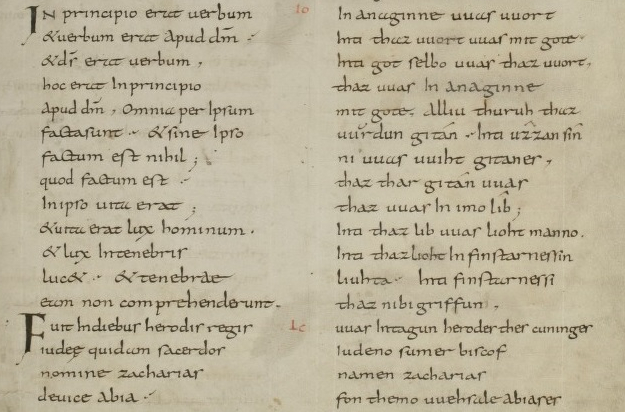
\includegraphics[width=10 cm]{images/tatian-handschrift-ausschnitt.jpg}
\caption {Auszug aus dem Tatian (\extrans{am Anfang war das Wort...})}
\label{abb:tatian-hand}
\end{center}
\end{figure} 

%In schwarz-weiß: images/tatian-handschrift-ausschnitt-sw.jpg

% http://www.e-codices.unifr.ch/de/csg/0056/25/0/Sequence-262
%% Verwendung: http://www.e-codices.unifr.ch/de/about/terms
%% nicht kommerziell mit cc-by; kommerziell bedarf schriftlicher Genehmigung
%% Ort, + Bibliothek, + Signatur, + Seitenzahl (www.e-codices.unifr.ch).
% Beispiel: 
% Engelberg, Stiftsbibliothek, Cod. 14, f. 12r (www.e-codices.unifr.ch).

Im Gegensatz zu dem ahd. Isidor und den Monseer Fragmenten wird der Ta"-ti"-an-Bi"-ling"-ue eine relativ starke Lateinabhängigkeit attestiert \parencites(){Lippert1974}[128]{Sonderegger2003}. Das Paradebeispiel für den lat. Einfluss ist der Umgang mit dem Ablativus absolutus. Die Konstruktion wird im Tatian fast immer in eine parallele Dativform überführt -- eine Strategie, die in den anderen ahd. Schriftstücken kaum zu beobachten ist \parencite[145f]{Lippert1974}. Daher kann man davon ausgehen, dass es sich bei diesem \hervor{absoluten Dativ} um eine nicht genuin ahd. Struktur handelt \parencite[zur vertiefenden Diskussion s.][39--40]{Fleischer2011}. Solche Strukturen imitieren also die lat. Syntax und sind außerdem dem Übersetzungszwang geschuldet, die Zeilengrenzen nicht zu überschreiten \parencite[136]{Masser1997}. Da Funktionswörter wie Subjektspronomen \is{Subjekt}\is{Personalpronomen}und auch das Artikelwort \object{dër} die exakte Zeilenübernahme kaum beeinträchtigen, werden grammatische \hervor{Kleinwörter} \parencite[43]{Fleischer2011} auch abweichend vom Original gesetzt \parencites[vgl. auch][20]{Dittmer1998}, so dass in diesen Fällen der Einfluss der lateinischen Syntax eher gering ist.  
Ein Weg, um sicherzugehen, dass es sich bei den Übersetzungen um \textit{echte} ahd. Strukturen handelt, ist das sog. Differenzprinzip, welches insbesondere in den jüngeren Arbeiten zum Tatian zum Einsatz kommt. Hierbei werden nur die von der Vorlage abweichenden Belege analysiert \parencite{Dittmer1998,Hinterholzl2005,Fleischer2008}. In der vorliegenden Arbeit werden Abweichungen von der lat. Vorlage ebenfalls gekennzeichnet (zum Vorgehen s. ausführlich Abschnitt \ref{sec:differenz}), so dass eine separate Analyse der Differenzbelege \is{Differenzbeleg} möglich ist.  


\subsection{Otfrids Evangelienbuch}

Otfrid von Weißenburg gilt als \blockcquote[146]{Sonderegger2003}{erste große, rein dichterische Gestalt des Ahd.}. Mit seiner Evangelienharmonie (nachfolgend auch als \hervor{(ahd.) Otfrid} bezeichnet) liegt uns ein ausgesprochen langes und gut überliefertes autochthones Textdenkmal vor. Als Entstehungszeit werden die Jahre 863--871 angenommen; Entstehungsort ist das Kloster Weißenburg im Elsass \parencite[50]{Fleischer2011}. Es handelt sich also um ein südrheinfränkisches Schriftstück. Ahnlich wie im ahd. Tatian wird auch in Otfrids Evangelienharmonie das Leben von Jesus Christus nacherzählt -- allerdings in Form eines poetischen Textes: Die Verse sind durch Endreim \is{Reim} miteinander verbunden   \parencite[zu Variationen im Versmaß s. ausführlich][148--150] {Sonderegger2003}; vgl. zur Illustration den Ausschnitt in Abbildung~\ref{abb:otfrid-hand}.\footnote{Herzog August Bibliothek Wolfenbüttel: Cod. Guelf. 131 Extrav.; \url{http://diglib.hab.de/mss/131-1-extrav/start.htm?image=00007}; zuletzt aufgerufen am 12.05.2020.}


\begin{figure}[h]
\begin{center}
  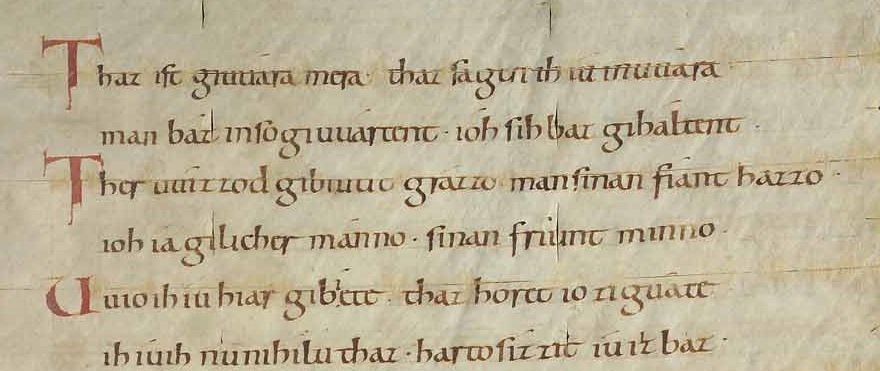
\includegraphics[width=10 cm]{images/otfrid-handschrift-ausschnitt.jpg}
  \caption {Die Anfangszeilen von Otfrids Evangelienbuch}
\label{abb:otfrid-hand}
\end{center}
\end{figure} 

% In schwarz-weiß: images/otfrid-handschrift-ausschnitt-sw.jpg

%http://diglib.hab.de/mss/131-1-extrav/start.htm?image=00007
% Nutzung: CC-BY-SA
% http://diglib.hab.de/copyright.html

Für syntaktische Untersuchungen ist der Text nicht ganz unproblematisch, da die Sprache an vielen Stellen durch Reim und Metrik beeinflusst wird. Ein eindeutiges Ergebnis von  Reimzwang \is{Reim} sind \textcite[35--36]{Fleischer2006} zufolge z.B. Kongruenzformen von Partizip\,+\,\object{wësan}, die ausschließlich bei Otfrid zu beobachten sind \parencites()()[s. auch][52]{Fleischer2011}[]{Gillmann2016}. 
Die \isi{Wortstellung} ist oft rhythmischen Prinzipien untergeordnet: So stehen attributive Adjektive \is{Adjektiv} und \isi{Determinierer} häufiger als in anderen Schriftstücken postnominal \parencites()()[282--283]{Oubouzar1989}[29]{Schrodt2004}. Und auch bei der Setzung von \object{dër} dürfen metrische \is{Metrik} Gründe (ähnlich wie  \textcite{Eggenberger1961} sie etwa für den Gebrauch des \is{Personalpronomen} Sub"-jekts"-pronomen postuliert) nicht ausgeschlossen werden. Wie \textcite[37]{Fleischer2006} anmerkt, ist es allerdings schwierig, diese stilistischen Einflüsse methodisch aufzuspüren. In der vorliegenden Untersuchung werden Reim \is{Reim} und \isi{Metrik} daher als mögliche Ursachen für Auffälligkeiten in der \isi{Nominalsyntax} gewertet, aber nicht explizit als Variablen annotiert. Was die Analyse der funktionalen Spannweite von \object{dër} angeht, ist Otfrids Evangelienbuch sehr gut geeignet, da keine lateinischen Interferenzen die Sprache beeinflussen. 

\subsection{Notkers Boethius} \label{sec:notker}

Notker III. (auch: Notker Labeo) ist Urheber der umfangreichsten Textsammlung, die aus dem späten Ahd. überliefert ist \parencites[157]{Meineke2001}. In seiner Rolle als Lehrer an der Klosterschule St. Gallen übertrug Notker nicht nur theologische, sondern auch wissenschaftliche und philosophische Texte aus der Antike ins Althochdeutsche und zwar mit dem Ziel, daraus Lese- und Interpretationsgrundlagen zu schaffen \parencite[zur Übersicht s.][136]{Sonderegger2003}. Für die nachfolgende Untersuchung wird Buch 1 und 2 von Notkers Boethius-Übersetzung \hervor{De consolatione Philosophiae} als Textgrundlage gewählt. Es handelt sich hierbei um einen Dialog zwischen dem Autor Boethius (5.--6. Jh.) und der personifizierten Philosophie \parencite[vgl.][]{Gruber2006}, der um 1025 von Notker übersetzt wurde \parencite[138]{Sonderegger2003}. 
In Abbildung~\ref{abb:notker-hand}\footnote{St. Gallen, Stiftsbibliothek, Cod. Sang. 825, p. 6 – Boethius, De consolatione philosophiae; \url{https://www.e-codices.ch/de/csg/0825/6/0/Sequence-673}; zuletzt aufgerufen am 12.02.2020.} sieht man, wie sich lateinische Grund- und althochdeutsche Zielsprache zeilenweise abwechseln.   

 \begin{figure}[h]
\begin{center}
  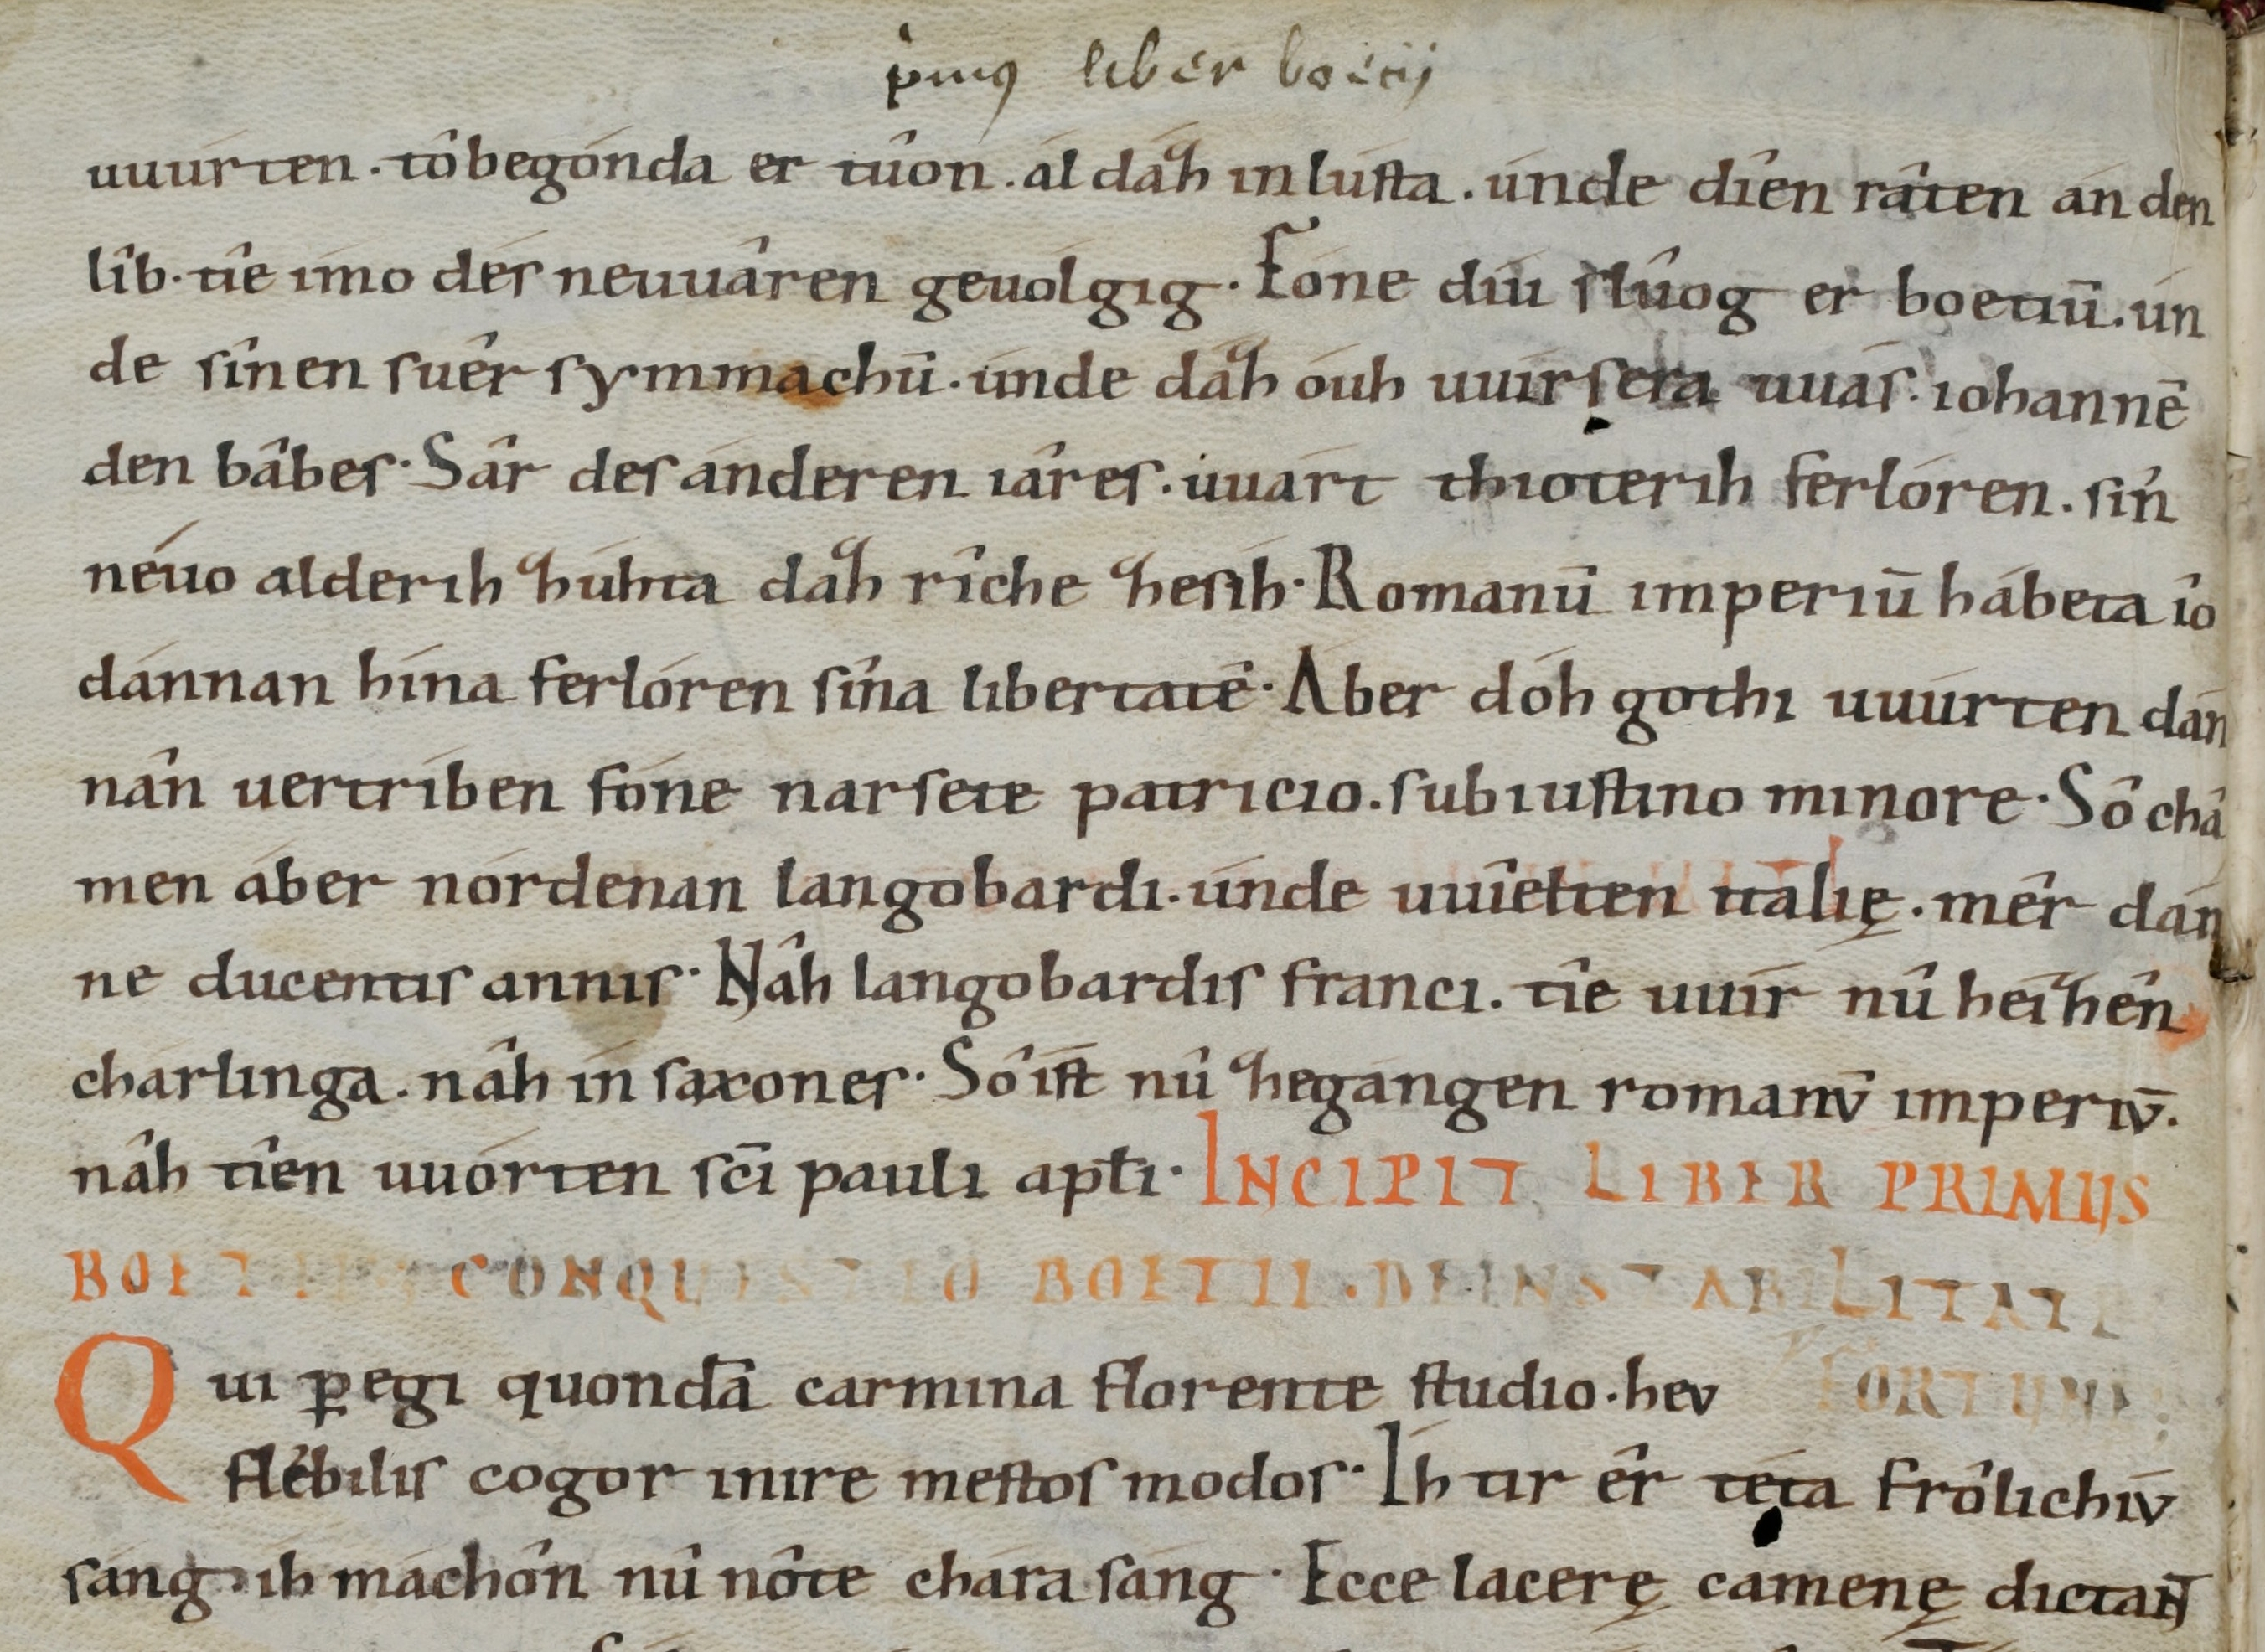
\includegraphics[width=10 cm]{images/notker-handschrift-buch1-ausschnitt.jpg}
\caption {Auszug aus Notkers Boethius, Buch 1}
\label{abb:notker-hand}
\end{center}
\end{figure} 

%In schwarz-weiß: notker-handschrift-buch1-ausschnitt-sw.jpg

Wie variabel Notker in seiner Übersetzung ist, dokumentiert die Studie von \textcite{Eilers2003}; zu Notkers Übersetzungstechnik s. auch \textcite{Glauch2003}. So werden bei der Übersetzung Satzteile oder ganze Sätze (vor allem Nebensätze) eingefügt, umgestellt oder auch getilgt, um ein besseres Textverständnis zu erzielen. Darüber hinaus ergänzt Notker die Vorlage mit eigenständigen ahd. Kommentaren. Um den ahd. Text im Lateinischen zu verankern, sind diese kommentierenden Passagen allerdings manchmal mit lat. Zitaten versetzt \parencite[vgl.][137]{Sonderegger2003}, was einem \blockcquote{Glaser2016}{mittelalterlichen Codeswitching} gleichkommt und die syntaktische Analyse erschwert.  


\section{Datenaufbereitung} \label{sec:datenaufbereitung}

Anders als in den bisherigen Studien zum \isi{Definitartikel} konnte bei der vorliegenden Untersuchung auf die annotierten Daten des \is{Korpus} \herkur{Referenzkorpus Altdeutsch} zugegriffen werden. Nachfolgend wird zunächst das \isi{Korpus} beschrieben (\ref{sec:ddd}) und dann erläutert, welche Schritte notwendig waren, um die Daten in ein weiterverarbeitbares Format zu überführen (\ref{sec:aufbereitung}). Der daran anschließende Abschnitt dokumentiert, auf welche Art und Weise die \isi{Annotation} vonstatten ging und welche Richtlinien \is{Annotationsrichtlinien} ihr zugrunde lagen (\ref{sec:annotationsschritte}).

\subsection{Das \object{Referenzkorpus Altdeutsch}} \label{sec:ddd}

Die in den vorhergehenden Abschnitten beschriebenen Texte sind über das \is{Korpus} \object{Referenzkorpus Altdeutsch} \parencite{Donhauser2015} zugänglich. In der vorliegenden Untersuchung wurde mit einer Vorversion von Version 0.1 des \isi{Korpus} gearbeitet \parencite{Donhauser2014}. Diese Version enthält neben den besagten Schriftstücken alle Textdenkmäler, die aus der althochdeutschen und altsächsischen Sprachperiode überliefert worden sind; die Texte beruhen auf handschriftennahen Editionen und umfassen etwa 300.000 Wortformen.
Die Texte wurden im Rahmen eines DFG-Projekts\footnote{Die Projektleitung für das DFG-geförderten Projekt (2008--2014) unterlag Karin Donhauser (HU Berlin), Jost Gippert (Frankfurt) und Rosemarie Lühr (Jena).} \is{Token}tokenisiert, \is{Lemma} lemmatisiert und übersetzt. Darüber hinaus sind sie nach Wortarten \is{Annotation} annotiert und mit flexionsmorphologischen \is{Flexion} Kategorien gekennzeichnet; neben \is{Token} tokenspezifischen Informationen (z.B. \isi{Kasus}, \isi{Numerus}) wurde auch die Flexionsklassenzugehörigkeit \is{Flexion} des Lemmas \is{Lemma} vermerkt (z.B. starke/schwache \isi{Flexion}). Zusätzlich liefert das \isi{Korpus} strukturelle Annotationen \is{Annotation} (Kapitel, Zeile, Vers etc.) zu den einzelnen Texten. 


\subsection{Export aus ELAN und Aufbereitung mit R}\label{sec:aufbereitung}

Um die ausgewählten Texte aus dem Altdeutschkorpus \is{Korpus} mit eigenen Annotationen \is{Annotation} anzureichern und die Belege statistisch auswerten zu können, mussten sie in ein bearbeitbares Format überführt werden. Für die vorliegende Untersuchung wurde das Dateiformat CSV gewählt. CSV-Dateien sind mit den meisten Programmen kompatibel und gewähren eine nachhaltige Datenspeicherung. 

Zum Zeitpunkt der Untersuchung (Anfang 2015) war es nicht möglich, die Texte in ihrer Gesamtheit als CSV-Dateien aus ANNIS3 \parencite{Krause2016}, der Plattform, über die die Texte öffentlich zugänglich sind, zu exportieren.\footnote{Über ANNIS3 kann man zwar Abfragen und Auswertungen durchführen, jedoch keine weiteren Annotationen \is{Annotation} hinzufügen oder komplexere Auswertungen (etwa statistische Tests) vornehmen, s. \url{https://korpling.german.hu-berlin.de/annis3/}; zuletzt aufgerufen am 12.02.2020.} Das Material wurde mir vom Altdeutsch-Projekt in Form von EAF-Dateien (=\,\object{ELAN Annotation Format}) zur Verfügung gestellt\footnote{Ein besonderer Dank gilt an dieser Stelle Martin Klotz für die Bereitstellung der Texte.}, welche mit ELAN\footnote{\url{https://tla.mpi.nl/tools/tla-tools/elan/}; zuletzt aufgerufen: am 12.02.2020.} in CSV-Dateien konvertiert werden konnten. 
Das Skript \hervor{aufbereitung-rohdaten.R} \parencite{HZKYL4_2020} dokumentiert, wie Fehler, die durch den Export entstanden sind, korrigiert wurden und welche weiteren Aufbereitungsschritte mithilfe von R\footnote{Version: 3.2.3 (2015-12-10); \url{https://www.R-project.org/}; zuletzt aufgerufen am 12.02.2020.} vorgenommen wurden. 
Um die Annotationen \is{Annotation} für Kongruenzabfragen und statistische Auswertungen zu nutzen, war es bspw. notwendig, die morphologischen Informationen aus dem \isi{Korpus} als einzelne Variablen \hervor{auszulagern}. So wurden im Altdeutsch-Projekt die adjektivischen \is{Adjektiv} Flexionskategorien in einer Variable (als String) \hervor{pos\_neut\_sg\_acc\_wk} annotiert. Diese fünf Kategorien (Komparation, \isi{Genus}, \isi{Numerus}, \isi{Kasus} und starke/schwache \isi{Flexion}) mussten gesplittet und in je eine neue Variable überführt werden. Außerdem wurden eine Reihe von Hilfsvariablen angelegt, um Strukturtypen \is{Nominalsyntax} der Nominalphrase \is{Nominalphrase (NP)} aus den Daten auslesen zu können; die entsprechenden Befehle sind ebenfalls in dem o.g. Skript aufgeführt.  

\subsection{Annotationsschritte}\label{sec:annotationsschritte}

Für die Untersuchung wurden folgende Ebenen \is{Annotation} annotiert: \isi{Belebtheit}, \isi{Relevanz}, \is{Semantische Rolle} semantische Rollen, Struktur der Nominalphrase \is{Nominalsyntax}\is{Nominalphrase (NP)}und \is{Definitheitskontext}Definitheitskontexte. Die \is{Belebtheit} Belebtheits- und Relevanzannotation \is{Relevanz}\is{Annotation}erfolgte auf Basis der Übersetzungen, die im Altdeutschkorpus \is{Korpus} bereitgestellt wurden (=\,Konzeptbasierte Annotation); die anderen Annotationen \is{Annotation} operierten auf den ahd. \isi{Token}  (=\,Tokenbasierte Annotation). Nachfolgend werden die Annotationstiefe \is{Annotation} sowie die einzelnen Schritte im Vorgehen erläutert, wobei die Belebtheitsannotation \is{Belebtheit}\is{Annotation}den methodischen Hauptteil der Arbeit darstellt und somit den größten Raum einnimmt. Der Leitfaden zur Annotation \is{Annotationsrichtlinien} der einzelnen Kategorien und die dazugehörigen Daten sind in \textcite{HZKYL4_2020} dokumentiert. 

%\subsubsection{(a) Belebtheit} 

Bislang sind in der Sprachwissenschaft kaum Studien zu finden, in denen authentische Daten systematisch nach \isi{Belebtheit} annotiert \is{Annotation} wurden und die somit als Vorbild für die komplexe  Belebtheitsannotation \is{Belebtheit}\is{Annotation}dienen könnten. Die Erkenntnisse sprachtypologischer Forschungen (vgl. Kapitel \ref{chapter:belebtheit}) basieren auf Einzelbelegen oder auf konstruierten Beispielen aus Grammatiken \parencite[z.B.][]{Comrie1989,Corbett2000,Aissen2003}. Die wenigen existierenden Korpusuntersuchungen  \parencite{Dahl1996,Yamamoto1999} machen keine Angaben, nach welchen Richtlinien annotiert \is{Annotation} wurde.

Pionierarbeit zur Belebtheitsannotation \is{Belebtheit}\is{Annotation}wurde im Bereich der historischen Linguistik im Rahmen des DFG-Projekts \hervor{Die Entwicklung der satzinternen Großschreibung im Deutschen (SiGS)} \parencite[vgl.][]{Szczepaniak2016} geleistet. Auf Basis der im Projekt ausgearbeiteten Richtlinien\footnote{Für die Bereitstellung danke ich Renata Szczepaniak und allen Mitarbeiterinnen und Mitarbeitern im SiGS-Projekt.} wurde eine eigene Anleitung zur Belebtheitsannotation \is{Belebtheit}\is{Annotation}für die vorliegende Untersuchung entwickelt. Darüber hinaus flossen die in Abschnitt \ref{sec:konabst} angesprochenen theoretischen Erkenntnisse zur Semantik von Substantiven \is{Substantiv} im Deutschen \parencite[u.a.][]{Ewald1992,Studler2011} in die Annotationsrichtlinien \is{Annotationsrichtlinien}sowie  Vorarbeiten aus der Computerlinguistik mit ein \parencite[vgl.][]{Garretson2004,Zaenen2004,Ovrelid2009}. Hier sind Belebtheitsannotationen \is{Belebtheit}\is{Annotation}bereits seit einigen Jahren Gegenstand des wissenschaftlichen Diskurses. Abbildung~\ref{abb:belebtheitsannotationsschema} gibt einen Überblick über die Kategorien, die bei der \isi{Annotation} unterschieden wurden.

\begin{sidewaysfigure}
\small
% % 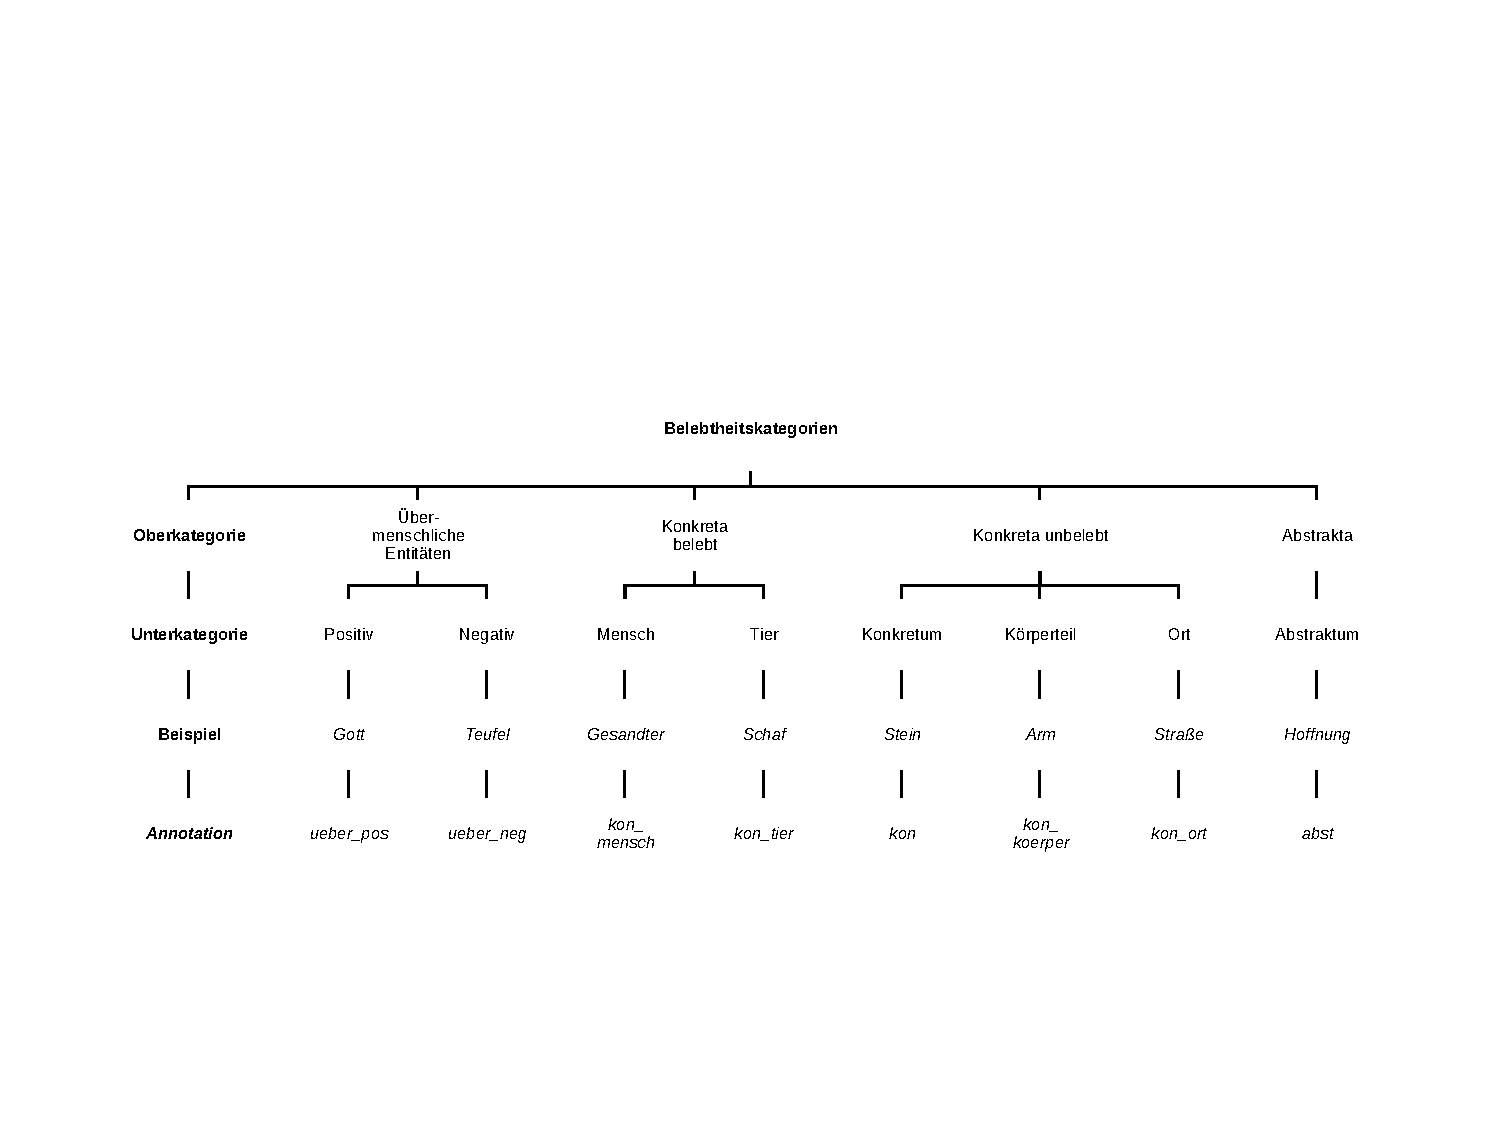
\includegraphics[width=\textwidth]{images/annotationsschema.pdf}
\begin{forest}
forked edges,for tree={fit=tight}
[Belebtheitskategorien,font=\bfseries
    [Oberkategorie,font=\bfseries,for descendants={font=\bfseries} 
                               [Unterkategorie [Beispiel [\itshape Annotation]]]]
    [Übermenschliche Entitäten [Positiv [\textit{Gott} [\textit{ueber\_pos}]]]
                               [Negativ [\textit{Teufel} [\textit{ueber\_neg}]]]
    ]
    [Konkreta belebt [Mensch [\textit{Gesandter} [\textit{kon\_mensch}]]]
                     [Tier [\textit{Schaf} [\textit{kon\_tier}]]]
    ]
    [Konkreta unbelebt [Konkretum [\textit{Stein} [\textit{kon}]]]
                       [Körperteil [\textit{Arm} [\textit{kon\_koerper}]]]
                       [Ort [\textit{Straße} [\textit{kon\_ort}]]]
    ]
    [Abstrakta [Abstraktum [\textit{Hoffnung} [\textit{abst}]]]]
]
\end{forest}
\caption {Belebtheitsannotationsschema\label{abb:belebtheitsannotationsschema}}
\end{sidewaysfigure} 

Vertikal abgebildet sind Ober- und Unterkategorien sowie dazugehörige Beispiele und die entsprechende \is{Annotation} Annotationskategorie. Horizontal zeigt sich die \isi{Belebtheitshierarchie}  und zwar absteigend von links [+belebt] nach rechts [\textminus{}belebt],  wobei teilweise weitere kognitive Faktoren die Unterteilung überlagern: So bildet die Hierarchie \is{Belebtheitshierarchie} auch Aspekte der kulturellen \isi{Relevanz} ab, da ganz links die sog. \object{übermenschlichen} Referenten stehen. Bezeichnungen für Orte sind prädestiniert dafür, eine niedrige \isi{Individualität} bzw. Spezifizität aufzuweisen, da sie oft als \isi{Adverbial} fungieren.\footnote{Bei den Konkreta \is{Konkretum} wurden darüber hinaus Körperteile gesondert \is{Annotation} annotiert. Diese Gruppe ist allerdings weniger für die \isi{Belebtheit} relevant, sondern in Bezug auf die Frage, inwiefern der emergierende Artikel bereits in nicht-demonstrativen Definitheitskontexten \is{Definitheitskontext} gebraucht wird (vgl. Abschnitt \ref{sec:pragsem}).} Viele Referenten sind -- wie die Ausführungen in Abschnitt \ref{sec:konabst} gezeigt haben~-- zwischen dem Pol [abstrakt] \is{Abstraktum} und [konkret] \is{Konkretum} anzusiedeln. Um dieser Gruppe gerecht zu werden, wurde eine Zwischenkategorie angesetzt. Der Belebtheitsleitfaden \is{Belebtheit}\is{Annotationsrichtlinien}enthält eine detaillierte Anleitung mit Beispielen, mit dem Ziel, eine möglichst objektive \is{Operationalisierung} Zuordnung zu gewährleisten.

Vor der \isi{Annotation} musste die Frage geklärt werden, ob \is{Lemma} lemma- oder token"-basiert annotiert \is{Annotation} wird. Für eine tokenbasierte \is{Token} \isi{Annotation} spricht, dass so auch Referenzverschiebungen \is{Referentialität} durch Metaphern \is{Metapher} und Metonymien \is{Metonymie} sowie kontextspezifische Interpretationen einbezogen werden können (\object{die Seiten im Buch} vs. \object{beide Seiten haben recht}). \textcite{Ovrelid2009} zeigt in einem Vergleich von \is{Lemma} Lemma- und \is{Token} Token\-annotation \is{Annotation} in schwedischen Wissenschaftstexten, dass solche Referenzverschiebungen mit 1,1\%  allerdings vergleichsweise selten sind.  Bei biblischen Texten, die naturgemäß einen höheren Anteil an Gleichnissen und metaphorischen \is{Metapher} Bezügen aufweisen, etwa falsche Propheten als \object{Wölfe} oder das Volk als \object{Schafsherde}, sieht die Verteilung jedoch vermutlich anders aus. 

Eine Art Kompromiss zwischen Lemma- und \is{Token} Tokenannotation \is{Annotation} ergibt sich,\linebreak wenn man die Übersetzungen, die im Altdeutsch-Projekt angefertigt wurden, als Annotationsgrundlage \is{Annotation} nimmt.  
Über den Internetauftritt des Projekts erfährt man: \hervor{Die Ebene \object{translation} enthält eine zum inhaltlichen Kontext des Lemmas passende Auswahl aus den bei \textcite{Splett1993} gegebenen Übersetzungsvorschlägen zum Lemma.}\footnote{\url{https://www.deutschdiachrondigital.de/manual/annotationsebenen}; zuletzt aufgerufen am 12.02.2020.} Konkret heißt dies, dass dasselbe Lemma je nach Kontext unterschiedlich übersetzt wurde.\footnote{Es muss angemerkt werden, dass -- wie mir Sonja Linde aus dem Projekt mitteilte -- die Übersetzungen nicht Teil der wissenschaftlichen Korpusarbeit waren und an vielen Stellen auch andere Lesarten möglich sind, da kein Leitfaden für die Übersetzungen entwickelt wurde. Eine systematische Kontextanalyse der ahd. \isi{Token} bleibt somit noch ein Forschungsdesiderat.} So wird das Lemma \object{wahsmo} in einigen Kontexten mit \extrans{Frucht} oder \extrans{Schößling, Sproß} übersetzt und verweist damit auf einen konkreten \is{Konkretum} Referenten. In anderen Fällen lautet die Übersetzung \extrans{Frucht, Kraft, Wachstum}, was einer  abstrakten \is{Abstraktum} (metaphorischen) \is{Metapher} Lesart von \object{wahsmo} Rechnung trägt. Umgekehrt kann ein und dieselbe Übersetzung, d.h. ein bestimmtes semantisches Konzept, für unterschiedliche Lemmata stehen, z.B. \hervor{Gleichnis} für ahd. \object{wortbilidi}, \object {gilīhnissi, gilīhnissī} oder \object{rātissa}. Indem man die Belebtheitsannotation \is{Belebtheit}\is{Annotation}auf Basis der Übersetzungen durchführt, kommt man einer kontextspezifischen Belebtheitsannotation \is{Belebtheit} \is{Annotation} also sehr nahe, vgl. zur Illustration Tabellen~\ref{tab:uem:1} und~\ref{tab:uem:2}. 
Ein wichtiger Vorteil dieser Annotationsform \is{Annotation} besteht zudem darin, dass große Datenmengen analysiert werden können, da nicht alle \isi{Token} einzeln annotiert \is{Annotation} werden müssen und die \isi{Annotation} auch ohne Althochdeutschkenntnisse erfolgen kann.

\vfill
\begin{table}[H]
\caption {Übersetzungsmöglichkeit im Altdeutschkorpus (1): Das gleiche Lemma wird unterschiedlich übersetzt.\label{tab:uem:1}}
\begin{tabular}{llll}
\lsptoprule
Token & Lemma & Übersetzung & Belebtheit\\\midrule
uuahsmo & \ldelim\{{3}{1em}[wahsmo] & Frucht & kon\\
uuahsmon & & Frucht, Kraft, Wachstum & abst\\
uuahsmon & & Schößling, Sproß & kon\\
\lspbottomrule
\end{tabular}
\end{table}
\vfill
\begin{table}[H]
\caption {Übersetzungsmöglichkeit im Altdeutschkorpus (2): Unterschiedliche Lemmata werden gleich übersetzt.\label{tab:uem:2}}
\begin{tabular}{llll}
\lsptoprule
\isi{Token} & Lemma & Übersetzung & Belebtheit\\\midrule
uuortbilidin & wortbilidi & \rdelim\}{3}{1em}[Gleichnis] & abst\\
gilihnessi & gilīhnissi, gilīhnissī &  & abst\\
ratissa & rātissa &  & abst\\
\lspbottomrule
\end{tabular}
\end{table}
\vfill
\pagebreak
% % % \begin{figure}
% % % \begin{center}
% % %   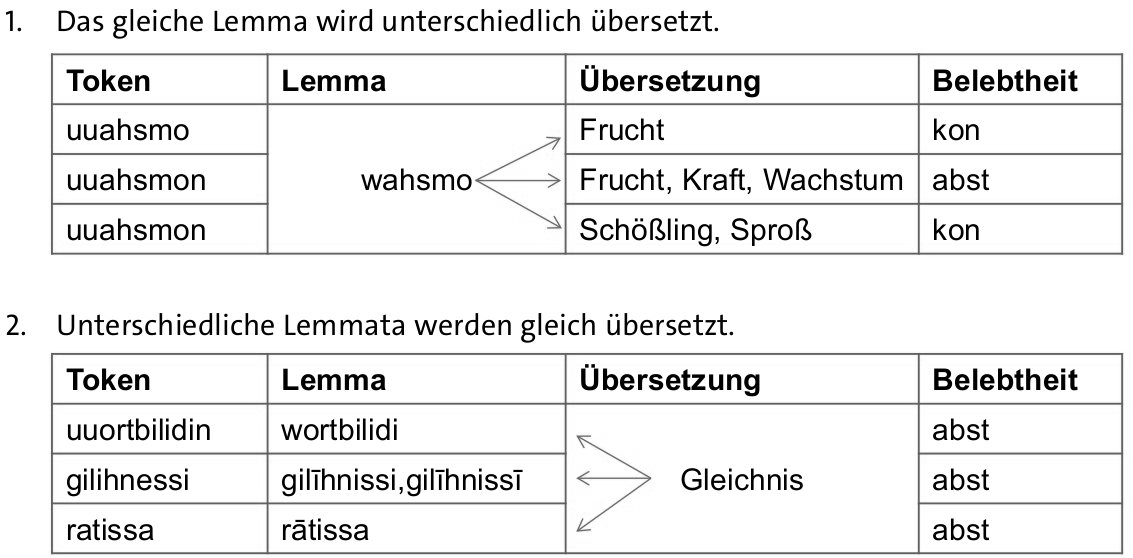
\includegraphics[width=10 cm]{images/konzept-ddd-sw.jpg}
% % % \caption {Übersetzungsmöglichkeiten im Altdeutschkorpus}
% % % \label{abb:konzept-ddd}
% % % \end{center}
% % % \end{figure} 
 

Der Annotationsprozess \is{Annotation} bestand aus einem zyklischen Wechsel von \isi{Annotation}, Eva"-lu"-ation, Ergebnisdiskussion und Anpassung des Leitfadens \parencite[entsprechend dem aus der Computerlinguistik bekannten \object{MAMA cycle} (=\,\herkur{Mod"-el-An"-no"-tate-Mo"-del-An"-no"-tate}), beschrieben u.a. in][109]{Pustejovsky2012}.

In einer Pilotstudie wurde eine Liste aller Übersetzungen \is{Type} (den Konzept-Types) erstellt, die entweder als Appellativa \is{Gattungsname} oder Eigennamen \is{Eigenname}  getaggt waren. Als Datengrundlage wurden der ahd. Isidor, der Tatian und Otfrids Evangelienharmonie genommen.  
Tabelle~\ref{tab:konzept-types} illustriert einen Ausschnitt der generierten Liste, welche 5195 Types \is{Type} umfasste. Die Länge der Liste resultierte nicht nur aus den unterschiedlichen Kontexten, sondern auch aus Variationen in der Zeichensetzung, z.B. Aufzählung mit Komma oder Semikolon, und Tippfehlern.  

\begin{table}
\centering
\begin{tabular}{l}
\lsptoprule
\multicolumn{1}{c}{Übersetzung (Konzept-Type)}    \\ \midrule
Bote                                        \\
Bote, (Ab)gesandter                         \\
Bote, Engel                                 \\
Bote, Gesandter                             \\
Bote, Herold                                \\
Bote, Herold, (Ab)gesandter, Apostel, Engel \\
Bote, Herold, (Ab)gesandter, Engel          \\
Bote, Herold, Engel                         \\
...                                         \\ \lspbottomrule
\end{tabular}
\caption{Ausschnitt aus der Konzept-Type-Liste\label{tab:konzept-types}}
\end{table}

Es folgte eine Probeannotation \is{Annotation} mit drei Annotatorinnen\footnote{Neben meiner Person waren dies Lisa Bürgerhoff und Jana Giesenschlag, für deren Hilfe ich mich an dieser Stelle herzlich bedanke.} auf Basis einer ersten Version des \is{Belebtheit}\is{Annotationsrichtlinien}Belebtheitsleitfadens. Ausgewählt wurden die ersten 508 Übersetzungen (von \object{Aas} bis \object{Bote}) aus der Liste; die \isi{Annotation} dauerte ca. 60 Minuten. Das \herkur{Inter Annotator Agreement} der drei Annotationen wurde mittels Fleiss' Kappa gemessen \parencite{Fleiss1971}. Das Maß nimmt Werte zwischen 0 und 1 an. 
0 steht für eine niedrige Übereinstimmung, die bei zufälliger \isi{Annotation} erwartbar wäre, 1 steht für perfekte Übereinstimmung. Zur detaillierteren Interpretation der Werte wurde die Skala von \textcite{Landis1977} herangezogen, s. Abbildung~\ref{abb:kappa-skala}.\footnote{Zu weiteren Interpretationsmöglichkeiten des Kappa-Koeffizienten vgl. die Diskussion in \textcite[576--577]{Artstein2008}.}

\begin{table}
\centering
\label{tab:iaa-pilot}
\begin{tabular}{lc}
\lsptoprule
Annotatorinnen & Fleiss' Kappa  \\ \midrule
A1 und A2               & 0,686  \\
A1 und A3               & 0,721  \\
A2 und A3               & 0,759  \\
A1, A2 und A3           & 0,722  \\ \lspbottomrule
\end{tabular}
\caption{\herkur{Inter Annotator Agreement} der Belebtheitsannotation (Pilotannotation mit drei Annotatorinnen)}
\end{table}

\begin{figure}
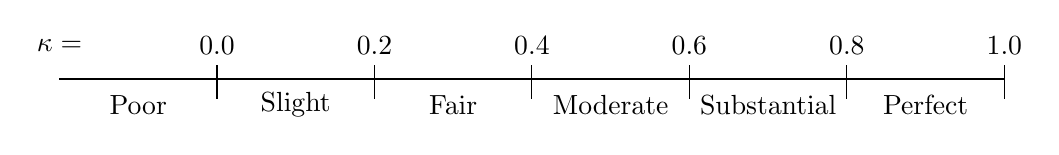
\begin{tikzpicture}[
        /pgf/number format/.cd,
		fixed,
		precision=1, 
		fixed zerofill,
		every node/.style={font=\strut}
    ]
	\node at (-2,0) {$\kappa=$};
	\draw (-2,-\baselineskip) -- (10,-\baselineskip);
	\foreach \i in {0,2,4,6,8,10}
		{
		   \node at (\i,0) {\pgfmathparse{\i/10}\pgfmathprintnumber{\pgfmathresult}};
		   \draw  (\i,-.25) -- ++(0,-\baselineskip);
		};
	\foreach \x/\y in {-1/Poor, 1/Slight, 3/Fair, 5/Moderate, 7/Substantial, 9/Perfect}
		{
		  \node at (\x,-.75) {\y};
		};
	\end{tikzpicture}
\caption {Kappa-Werte und Stärke der Übereinstimmung \parencite[576]{Artstein2008}\label{abb:kappa-skala}}
\end{figure} 

In diesem ersten Durchgang wurde mit einem Kappa-Wert von 0,722 (\herkur{substantial}) bereits eine relativ hohe Übereinstimmung zwischen den drei Annotationen \is{Annotation} erzielt, vgl. Abbildung~\ref{abb:kappa-skala}.\largerpage[1.25]
Nach einer intensiven Auseinandersetzung mit systematischen Fehlern\footnote{Zur Diskussion stand bspw., ob Körperflüssigkeiten als Körperteile zu definieren sind.} wurde der Leitfaden überarbeitet und erneut ca. 500 Konzept-Types \is{Type} doppelt \is{Annotation} annotiert. Diesmal geschah die \isi{Annotation} allerdings unter Ausschluss von \is{Eigenname} Eigennamen, weil diese für die spätere Analyse wenig relevant sind, aber einen relativ großen Teil der Konzept-Type-Liste \is{Type} ausgemacht haben und für eine hohe Übereinstimmung sorgten. Denn Eigennamen \is{Eigenname} verweisen meist auf eindeutig menschliche Referenten (etwa \object{Andreas, Aaron}) oder Städte (z.B. \object{Babylon, Bethlehem}).
Ihr Wegfall hatte dann vermutlich zur Folge, dass beim zweiten Durchgang der Kappa-Wert mit 0,552 deutlich unter dem ersten Wert lag. 
Die Konfusionsmatrix in Abbildung~\ref{abb:confusion} zeigt, dass im zweiten Durchgang vor allem zwischen den\is{Abstraktum}  Abstrakta, den Konkreta \is{Konkretum} und der Zwischenkategorie \hervor{abstrakt/konkret} \is{Konkretum}\is{Abstraktum}Uneinigkeit herrschte. Vermutlich ist der Kappa-Wert bei \textcite{Zaenen2004} höher (sie erzielten bei ihrer Belebtheitsannotation \is{Belebtheit}\is{Annotation}einen Wert über 0,9), weil sie nur zwischen prototypisch konkret \is{Konkretum} und nicht-konkret differenzieren. Man sieht auch, dass Annotatorin 1 (horizontal) entscheidungsfreudiger war als Annotatorin 2 (vertikal), da letztere häufiger ein \hervor{unklar} vergab. Interessant ist hier die Kategorie \hervor{kon\_ort}, in welche Annotatorin 1 Konzept-Types \is{Type} wie \object{Erde, Haus}, \object{Erde, Gebiet} oder \object{Einöde, Wüste} eingeordnet hat, während von Annotatorin 2 hier \hervor{abst\_kon} oder \hervor{abst} annotiert wurde. In Zukunft könnte man durch eine intensive \hervor{Fehler}-Analyse solcher Annotationsdurchgänge \is{Annotation} weitere Erkenntnisse für Belebtheitsannotationen \is{Belebtheit} \is{Annotation} ableiten.  
 
\begin{figure}
\begin{center}
  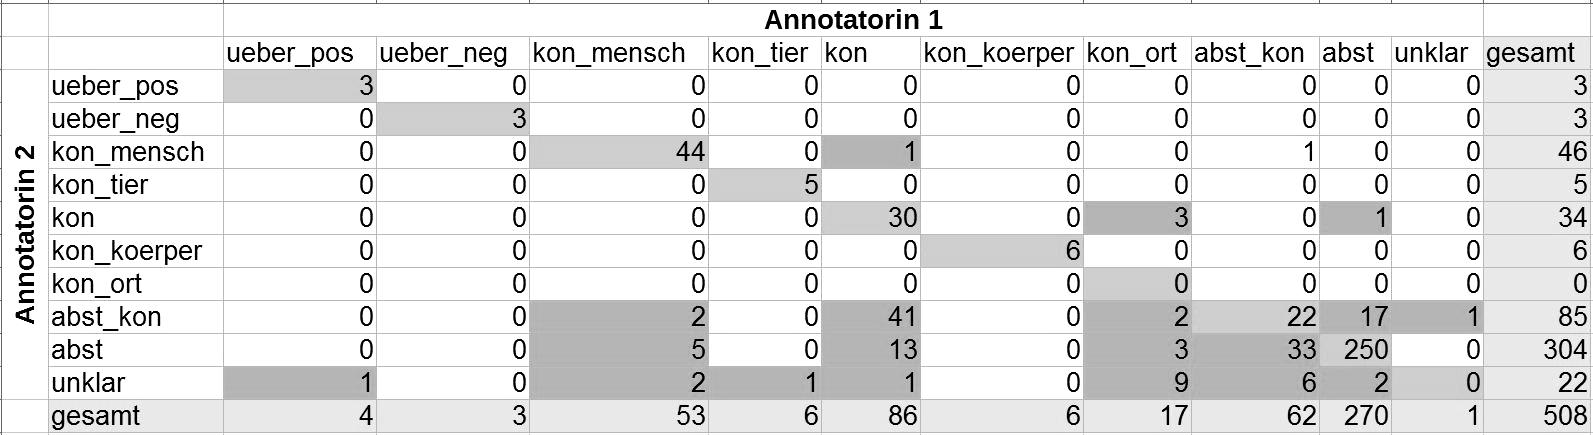
\includegraphics[width=\textwidth]{images/confusionsmatrix-neu-sw.jpg}
\caption {Konfusionsmatrix für die zweite Annotationsrunde}
\label{abb:confusion}
\end{center}
\end{figure} 

Für den dritten und letzten Annotationsdurchgang \is{Annotation} wurde der Leitfaden erneut leicht angepasst.\footnote{Die finale Version des Leitfadens liegt in \textcite{HZKYL4_2020} ab.} Die Konzeptliste wurde nach dem Modell des vorhergehenden Durchgangs (also ohne \is{Eigenname} Eigennamen), aber diesmal auf Basis aller zu untersuchenden Texte (s. Abschnitt \ref{sec:textauswahl}), erstellt (=\,15.039 Types) \is{Type} und doppelt \is{Annotation} annotiert.\footnote{Da auch Buchstaben oder Satzzeichen unter der Liste zu finden waren, wurden diese vor der \isi{Annotation} mit \hervor{keine Angabe} gekennzeichnet.} Der neue Kappa-Wert lag bei 0,701. Übersetzungen, die aus Verständnisgründen als \hervor{unklar} klassifiziert wurden und deswegen nicht nach \isi{Belebtheit} annotiert \is{Annotation} werden konnten, wurden von mir mit Erklärungen versehen und anschließend erneut zur \isi{Annotation} freigegeben. Der Kappa-Wert veränderte sich hierdurch nur unwesentlich (0,688); insgesamt ist die Übereinstimmung mit Blick auf Abbildung~\ref{abb:kappa-skala} also als  \herkur{substantial} zu werten. Für die Auswertung wurden am Ende nur die Fälle einbezogen, bei denen beide Annotatorinnen übereinstimmten.

%\subsubsection{(b) Relevanz} 

Bei der Belebtheitsannotation \is{Belebtheit}\is{Annotation}wurde der Faktor \isi{Relevanz} mit der Kategorie \hervor{übermenschliche Entitäten} (s. Abbildung~\ref{abb:belebtheitsannotationsschema}) in Teilen schon abgedeckt. Um zu überprüfen, inwiefern das Geschlecht einen Einfluss auf den Artikelgebrauch hat, wurden zusätzlich alle menschlichen Konkreta \is{Konkretum} in \hervor{männlich} und \hervor{weiblich} unterteilt.\footnote{Bei dieser Aufgabe habe ich Unterstützung von Lisa Bürgerhoff erhalten.} 
Trotz der recht eindeutigen Dichotomie gibt es durchaus Fälle, die in die Klasse \hervor{unklar} fielen, z.B. \object{Mitbürger} oder \object{Altersgenossen}, welche bei der Analyse dann ausgespart wurden.  Die \isi{Annotation} erfolgte erneut konzeptbasiert, d.h. die Grundlage bildete eine automatisch generierte Liste der  Übersetzungen aus dem \is{Korpus} Altdeutschkorpus, die am Ende wieder mitsamt der \hervor{Geschlechtsannotation} \is{Annotation}den jeweiligen ahd. \isi{Token} zugeordnet wurden.\largerpage

%\subsubsection{(d) Struktur der Nominalphrase}
Um die Struktur der Nominalphrase \is{Nominalsyntax}\is{Nominalphrase (NP)}zu \is{Annotation} annotieren, wurde eine zufällige Stichprobe\footnote{Zum Vorgehen vgl. das R-Skript \hervor{aufbereitung-rohdaten.R} \parencite{HZKYL4_2020}.} (bestehend aus je 100 \is{Gattungsname} Appellativa) aus dem Isidor, dem Tatian und Otfrid genommen. Annotiert wurden Informationen zum Phrasentyp \is{Phrase} und zur Art und Anzahl von Determinierern \is{Determinierer} sowie \is{Genitivattribut}\is{Adjektiv}Attributen. Bei den Übersetzungstexten wurden zusätzlich das lateinische \isi{Token} und ggf. Abweichungen in der Struktur \is{Nominalsyntax} (Vorhandensein und \is{Wortstellung} Stellung von Determinierern \is{Determinierer} und Attributen) dokumentiert. Beim Tatian wurde zudem vermerkt, auf welche Bibelstelle der ahd. Text Bezug nimmt sowie eine Übersetzung davon angegeben. Außerdem gibt es bei der Annotation Raum für Anmerkungen und Übersetzungsprobleme.
%\subsubsection{(e) Definitheit} 
Jede der 100 NPs \is{Nominalphrase (NP)} aus der  Stichprobe wurde zusätzlich einem Definitheitskontext \is{Definitheitskontext} zugewiesen. Es wurden also nicht nur die \object{dër}-Belege nach ihrem Definitheitskontext \is{Definitheitskontext} (pragmatische \is{Pragmatische Definita}  oder semantische \is{Semantische Definita} Definitheit) analysiert, sondern auch alle Phrasen \is{Phrase} ohne \object{dër}, um diese anschließend vergleichen zu können. 
%Die Ausprägungen der Variable \hervor{Definitheit} sind in Tabelle~\ref{tab:definitheit} aufgelistet.
Die Kategorien basieren auf den Gebrauchskontexten, die in Kapitel \ref{chap:demdef} erläutert wurden. Fälle, die nicht eindeutig in eine der Kategorien passten, wurden als \hervor{ambig} gekennzeichnet und später als mögliche Brückenkontexte \is{Brückenkontext} separat analysiert. 
%\subsubsection{(c) Semantische Rollen} 
Was Art und Anzahl von semantischen Rollen \is{Semantische Rolle} angeht, die als Kandidaten für eine Annotation in Frage kommen, gilt es eine Auswahl aus der Vielzahl von Theorien (vgl. Abschnitt~\ref{sec:partizipanten}) zu treffen: Gerade bei historischen Texten stößt man mit jeder neuen Unterkategorie schnell an die Grenzen dessen, was operationalisierbar \is{Operationalisierung} und damit annotierbar \is{Annotation} ist. In der vorliegenden Arbeit wurden daher im Rahmen der \is{Annotation}\is{Nominalphrase (NP)}NP-Stichprobenannotation, Referenten ganz basal \is{Agentivität} in \hervor{Proto-Agens}, d.h. \is{Subjekt} Subjekte, die willentlich handeln,  eine Bewegung ausführen oder Träger eines Gefühlszustandes sind,  und \hervor{Nicht-Proto-Agens} unterteilt.

Alle in diesem Abschnitt genannten Kategorien sowie Erläuterungen zur Annotation \is{Annotation} sind in den \isi{Annotationsrichtlinien} \parencite{HZKYL4_2020} aufgeführt.  


% \begin{table}
% \centering
% \begin{tabular}{ll}
% \lsptoprule
% Annotation & Kurzbeschreibung  \\ \midrule
% situativ            & Situativer Bezug               \\
% anaphorisch         & Anaphorischer Bezug            \\
% diskurs             & Diskursdeiktischer Bezug      \\
% anamnestisch        & Anamnestischer Bezug           \\
% abstrakt            & Abstrakt-situativer Bezug      \\
% assoziativ          & Assoziativ-anaphorischer Bezug \\
% monoref             & Referent ist monoreferent      \\
% generisch           & Generische Lesart              \\
% nicht-spezifisch        & Unspezifischer Referent           \\
% spezifisch-indefinit          & Spezifischer Referent           \\
% indefinit           & Indefinita     \\
% possessiv           & Possessiver Bezug    \\
% ambig\_kat1\_kat2  & Ambige/Uneindeutige Fälle      \\ \lspbottomrule
% \end{tabular}
% \caption{Annotationsmöglichkeiten für die Variable \hervor{Definitheit}\label{tab:definitheit}}
% \end{table}

\section{Analysemethoden} \label{sec:analysemethoden}

Die Untersuchung fußt auf zwei unterschiedlichen Analysemethoden. Zum einen wurden die in \ref{sec:textauswahl} beschriebenen Texte in ihrer Gesamtheit untersucht, und zwar mithilfe der im Referenzkorpus Altdeutsch \is{Korpus} vorhandenen \is{Annotation} Annotationen. Die Daten wurden hierbei nach Einheiten durchsucht, die stellvertretend für das spezifische sprachliche Phänomen stehen, sog. Proxys \is{Proxy} \parencite[vgl.][114]{Lemnitzer2015}, s. zur Illustration Tabelle~\ref{tab:proxys}. Die Auswahl spezifischer Lemmata, etwa Unika \is{Unikum} wie \object{sunna} \extrans{Sonne}, orientiert sich an den manuell durchgeführten Vorarbeiten zum Artikelgebrauch. Besonders hervorzuheben sind die Untersuchungen von \textcite{Graf1905}, \textcite{Bell1907}, \textcite{Hodler1954} und \textcite{Oubouzar1989}: Hier wurde das ahd. Datenmaterial von Hand nach Belegen durchforstet und ausgezählt. Sie dienen damit als wichtige Referenzquelle für die vorliegende computergestützte Auswertung. 

Zum anderen wurden die Korpusdaten mit eigenen Annotationen \is{Annotation} angereichert; die Kategorien wurden im vorhergehenden Abschnitt beschrieben. Die Belebtheitsannotation \is{Belebtheit}\is{Annotation}ist so konzipiert, dass sie für eine ganzheitliche Analyse geeignet ist, d.h. alle Appellativa \is{Gattungsname} können nach \isi{Belebtheit} ausgewertet werden. Die Mehrebenen-Annotation \is{Annotation} zur \is{Nominalphrase (NP)} NP, den Definitheitskontexten \is{Definitheitskontext} und den semantischen Rollen \is{Semantische Rolle} beschränkt sich gemäß ihrer Komplexität und des damit verbundenen Zeitaufwands auf zufällige Stichproben. Bei der Ergebnispräsentation wird jeweils vermerkt, ob die Daten auf Auswertungen des gesamten \isi{Korpus} oder Stichprobenanalysen basieren. 

\begin{table}
\centering
\begin{tabular}{ll}
\lsptoprule
Kategorie     & Proxy            \\ \midrule
Semantische Definitheit\is{Semantische Definita} & Superlative, \is{Unikum}\is{Superlativ}Unika            \\
Definite NP \is{Nominalphrase (NP)}  & Definite Artikelformen\,+\,Nomina Appellativa \is{Gattungsname}       \\
Niedrige \isi{Individualität} & \isi{Massennomen}, Belege im Plural \is{Numerus} \\ \lspbottomrule
\end{tabular}
\caption{\isi{Operationalisierung} unterschiedlicher Kategorien durch \is{Proxy} Proxys\label{tab:proxys}}
\end{table}
 
\subsection{Qualitative und quantitative Analysen}\label{sec:qual-quant}

Im Normalfall setzen quantitative Auswertungen immer qualitative Entscheidungen voraus.\footnote{Ausnahmen sind Bottom-up-Analysen, die nahezu ohne Einspeisung von theoriegeleitetem Wissen arbeiten, z.B. mithilfe von N-Gramm-Auswertungen wie etwa bei \textcite{Scharloth2012}.} So muss jegliche Information, die ein \isi{Korpus} zusätzlich zum reinen Primärtext enthält \is{Token} (Tokenisierung, PoS-Tags, morphologische Auszeichnungen, \is{Belebtheit} Belebtheitskategorien, Übersetzungen, Meta-Daten etc.) zuvor eindeutig definiert und ggf. für die \isi{Annotation} operationalisiert \is{Operationalisierung} werden. Erst dann können die Belege gemäß der Kategorien, in die sie eingeordnet wurden, ausgezählt und statistisch miteinander verglichen werden.   

In der vorliegenden Arbeit basieren die quantitativen Auswertungen auf unterschiedlichen Arten der qualitativen Vorarbeit:
Eine wichtige Grundlage für die Untersuchung bilden die PoS-Annotationen \is{Annotation} und die morphologischen Informationen, die das Altdeutschkorpus \is{Korpus} bereitstellt.\footnote{Zur Übersicht der Kategorien s. \url{https://www.deutschdiachrondigital.de/manual/annotationsebenen}; zuletzt aufgerufen am 12.02.2020.} Durch sie können bspw. alle Nomen Appellativa \is{Gattungsname} (NAs), denen ein kongruentes \is{Flexion} \object{dër} (DDA) vorhergeht, ausgezählt werden.
Zudem lassen sich mithilfe der Annotationen \is{Annotation} sprachliche Muster aufdecken, etwa Kombinationsmöglichkeiten von stark oder schwach flektierten Adjektiven \is{Flexion}\is{Adjektiv}mit \object{dër}. Die einheitliche \is{Lemma} Lemmatisierung der Texte kann für Stichprobenanalysen genutzt werden, etwa um Gebrauchsunterschiede von ausgewählten Nomen \is{Substantiv} herauszuarbeiten. So wird der Einfluss von \isi{Individualität} auf die Artikelsetzung z.B. an \isi{Massennomen} im Vergleich zu zählbaren Nomen \is{Substantiv}\is{Numerus}sichtbar.

Die konzeptbasierte Belebtheitsannotation \is{Belebtheit}\is{Annotation}gewährleistet ebenfalls eine globale Analyse der Texte, da jedem Appellativum \is{Gattungsname} ein Belebtheitsgrad \is{Belebtheit} zugeordnet wird. Auf diese Weise kann der Einfluss der Variable \isi{Belebtheit} auf die Artikelsetzung überprüft werden. 

Ergänzend zur Analyse der NP-Struktur \is{Nominalphrase (NP)}\is{Nominalsyntax}durch Proxys \is{Proxy} werden Auswertungen vorgenommen, die auf einer eigenen qualitativen Analyse der NP \is{Nominalphrase (NP)} basieren (s. Abschnitt \ref{sec:annotationsschritte}). Das ahd. Wörterbuch von \textcite{Schutzeichel2012} sowie bisherige Analysen zum ahd. \object{dër} \parencite[v.a.][]{Oubouzar1989} dienen hierbei als Verständnishilfe.  

Um den Einfluss der einzelnen Kategorien auf die Verwendung von \object{dër} zu testen, wurden statistische Signifikanztests ($\chi^2$-Test sowie Exakter Test nach Fisher) und Residuenanalysen (mithilfe von Mosaikplots) durchgeführt \parencite{Gries2012}. Das Signifikanzniveau wurde auf 0,05 angesetzt.

\subsection{Umgang mit Differenzbelegen}\label{sec:differenz}

Differenzbelege \is{Differenzbeleg} können nicht automatisch, sondern nur manuell klassifiziert\linebreak werden, da zum Zeitpunkt der Untersuchung keine digitale Alignierung von lat. und ahd. Texten vorliegt. Bei der Stichprobenanalyse zur Struktur \is{Nominalsyntax} der NP \is{Nominalphrase (NP)} wurde daher jeder Beleg mit der lateinischen Vorlage von Hand abgeglichen. Alle für die Fragestellung relevanten morphosyntaktischen Abweichungen wurden dokumentiert. Die wichtigsten betreffen a) die Setzung von ahd. \object{dër} und die Frage, ob dies durch ein lateinisches \isi{Demonstrativum} (v.a. \object{ille}) motiviert sein könnte und b) die Frage nach der Nominalsyntax: Gibt es Stellungsunterschiede \is{Wortstellung} bei \is{Determinierer} Determinierern oder \is{Genitivattribut}\is{Adjektiv}Attributen? Für den ahd. Tatian wurde die Edition von Sievers (1966) genutzt, die online über Titus\footnote{\url{http://titus.uni-frankfurt.de/texte/etcs/germ/ahd/tatian/tatia.htm}; zuletzt aufgerufen am 12.02.2020.} eingesehen werden kann. Beim ahd. Isidor konnte auf die lateinische Version im Altdeutschkorpus \is{Korpus} (Eggers 1964) Bezug genommen werden.  


\section{Zusammenfassung}

In diesem Kapitel wurde gezeigt, wie die Struktur [\object{dër}\,+\,N] im Althochdeutschen über korpuslinguistische \is{Korpuslinguistik} Methoden analysiert werden kann. Folgende Texte, deren Herkunft und sprachliche Besonderheiten dargelegt wurden, liegen der Untersuchung zugrunde: Isidor (um 790), Monseer Matthäus (um 810), Tatian (um 840), Otfrids Evangelienbuch (um 870) und Notkers Boethius (1025). Sie wurden im Rahmen des \object{Referenzkorpus Altdeutsch}-Projekt \is{Korpus} mit grammatischen Informationen (u.a. Wortarten und \is{Flexion} Flexionskategorien) ausgezeichnet, was eine systematische Suche nach der Zielstruktur [\object{dër}\,+\,N] sowie nach weiteren, für die Fragestellung relevanten Belegstellen, darunter bestimmte \is{Unikum} Unika, Superlative \is{Superlativ} und Kombinationen von \object{dër}\,+\,Adjektiv \is{Adjektiv} ermöglicht. Das methodische Herzstück der Arbeit ist die \is{Annotation}\is{Belebtheit}Belebtheitsannotation, welche in diesem Kapitel schrittweise erläutert wurde. Um eine möglichst objektive \is{Operationalisierung} Zuweisung der einzelnen Belebtheitsgrade bei den Substantiven \is{Substantiv} zu erreichen, wurde ein Annotationsleitfaden \is{Annotationsrichtlinien} erstellt und die einzelnen \is{Annotation} Annotationsdurchgänge über \herkur{Inter Annotator Agreements} evaluiert. Auch für die anderen Analysekategorien (\isi{Definitheit}, Struktur der \is{Nominalphrase (NP)} NP, semantische \is{Semantische Rolle} Rollen) liegen Richtlinien vor, die im Anhang \parencite{HZKYL4_2020} der Arbeit einzusehen sind. Weil es sich bei einigen Texten um Übersetzungen aus dem Lateinischen handelt, werden auch \is{Differenzbeleg} Differenzbelege, d.h. \object{dër}-Setzungen  und \is{Wortstellung} Wortstellungsabfolgen, die von der Vorlage abweichen, gekennzeichnet und separat analysiert. 
  

%\chapter{Ergebnisse}\label{ergebnisse}

In diesem Kapitel werden die Ergebnisse der Korpusuntersuchung \is{Korpus} präsentiert. Um eine Übersicht über die Gebrauchsfrequenz von adnominalem \object{dër} zu bekommen, liefert Abschnitt \ref{sec:ergeb-ther-freq} eine Gegenüberstellung aller Phrasen mit und ohne \object{dër}. Anschließend widmet sich Abschnitt~\ref{sec:ergeb-definitheit} dem funktionalen Spektrum von \object{dër}, indem zunächst die Ergebnisse zur Stichprobenanalyse dargestellt werden (je 100 NPs wurden im Isidor, Tatian und Otfrids Evangelienbuch nach Definitheitskontexten \is{Definitheitskontext} klassifiziert). Anschließend wird die Distribution von \object{dër} bei ausgewählten Unika \is{Unikum} sowie Superlativkonstruktionen \is{Superlativ} offengelegt. In Abschnitt~\ref{sec:ergeb-faktoren} zeigt sich, welche Korrelationen es zwischen dem Gebrauch von \object{dër} und den kognitiven Faktoren \isi{Belebtheit}, \isi{Individualität}, \isi{Relevanz} sowie \isi{Agentivität} gibt. 
Im Anschluss dokumentiert Abschnitt~\ref{erg:struktur.np} die Struktur der \is{Nominalphrase (NP)} Nominalphrase. Die Ergebnisse liegen u.a. einer Proxysuche \is{Proxy} nach spezifischen Strukturtypen zugrunde, die zu Beginn des Abschnitts erläutert werden. Es wird hier auch überprüft, wie das Stellungsverhalten \is{Wortstellung} von \object{dër} und anderen Determinierern \is{Determinierer} ausfällt. Zudem werden Korrelationen von Adjektivflexion \is{Flexion}\is{Adjektiv}und \object{dër}-Setzung offengelegt. 

\section{Überblick: Frequenz von [\object{dër}\,+\,N]}\label{sec:ergeb-ther-freq}\largerpage

Tabelle~\ref{tab:ther-freq-abs} zeigt die absoluten Häufigkeiten von \object{dër} in den fünf untersuchten Texten; in Tabelle~\ref{tab:ther-freq-rel} sieht man die entsprechenden relativen Werte. Hierbei wird noch nicht zwischen \object{dër} als De"-mon"-strativ-"- \is{Demonstrativartikel} oder \isi{Definitartikel} unterschieden. Auf diese funktionalen Differenzen wird in Abschnitt \ref{sec:ergeb-definitheit} eingegangen. Die Ergebnisse beruhen auf folgender \isi{Operationalisierung}: In den Texten wurden alle \isi{Token} mit dem PoS-Tag \hervor{NA} (=\,Nomen \is{Gattungsname} Appellativum) gesucht und anschließend ermittelt, ob den einzelnden NAs ein  \object{dër} unmittelbar oder im  Abstand von max. einem \isi{Token} vorausgeht. Dabei wurde darauf geachtet, dass Nomen und Determinierer \is{Determinierer} in \isi{Kasus}, \isi{Numerus} und \isi{Genus} übereinstimmen. Die Häufigkeiten in der Zeile \hervor{NAs \is{Gattungsname} mit \object{dër}} repräsentieren entsprechend zwei Strukturtypen:\footnote{In der Tabelle zusammengefasst als \object{dër} (+ \_\_ ) NA.}  
%\footnote{Nachfolgend werden folgende Abkürzungen (vgl. auch Abschnitt \ref{sec:textauswahl}) verwendet: Isidor (I), Monseer Matthäus (M), Tatian (T), Otfrid (O) und Notker (N).}

\begin{itemize}
\item[a.] [\object{dër}\,+\,Nomen Appellativum], z.B. \object{ther forasago}
\item[b.] [\object{dër}\,+\,X\,+\,Nomen Appellativum],
z.B. \object{ther heilac geist} % schreibung nachgucken
\end{itemize}

% R-script: NA-artikel #2
\begin{table}
\centering
% latex table generated in R 3.2.3 by xtable 1.8-2 package
% Fri Feb  3 11:30:15 2017
\begin{tabular}{rrrrrr}
  \hline
 \textbf{Struktur} & \textbf{I (790)} & \textbf{M (810)} & \textbf{T (840)} & \textbf{O (870)} & \textbf{N (1025)} \\ 
  \hline
NAs mit \object{dër} & 189 & 125 & 1446 & 2839 & 617 \\ 
  NAs ohne \object{dër} & 801 & 673 & 4569 & 6882 & 1604 \\ 
  Summe & 990 & 798 & 6015 & 9721 & 2221 \\ 
   \hline
\end{tabular}

\caption{Absolute Häufigkeiten von \object{dër} (+ \_\_ ) NA}
\label{tab:ther-freq-abs}
\end{table}

\begin{table}
\centering
% latex table generated in R 3.2.3 by xtable 1.8-2 package
% Fri Feb  3 11:30:15 2017
\begin{tabular}{rrrrrr}
 \lsptoprule
 {Struktur} & {I (790)} & {M (810)} & {T (840)} & {O (870)} & {N (1025)} \\ 
  \midrule
NAs mit \object{dër} & 19.10 & 15.70 & 24.00 & 29.20 & 27.80 \\ 
  NAs ohne \object{dër} & 80.90 & 84.30 & 76.00 & 70.80 & 72.20 \\ 
  Summe & 100.00 & 100.00 & 100.00 & 100.00 & 100.00 \\ 
   \lspbottomrule
\end{tabular}

\caption{Relative Häufigkeiten von \object{dër} (+ \_\_ ) NA}
\label{tab:ther-freq-rel}
\end{table}

Zum besseren Vergleich wurden die Daten aus Tabelle~\ref{tab:ther-freq-abs} und \ref{tab:ther-freq-rel} in Abbildung~\ref{abb:art-freq} überführt.  

\vfill
% R-script: NA-artikel #1.1 Absolute Zahlen & #1.2 Relative Zahlen
\begin{figure}
\begin{subfigure}[b]{.5\linewidth}
  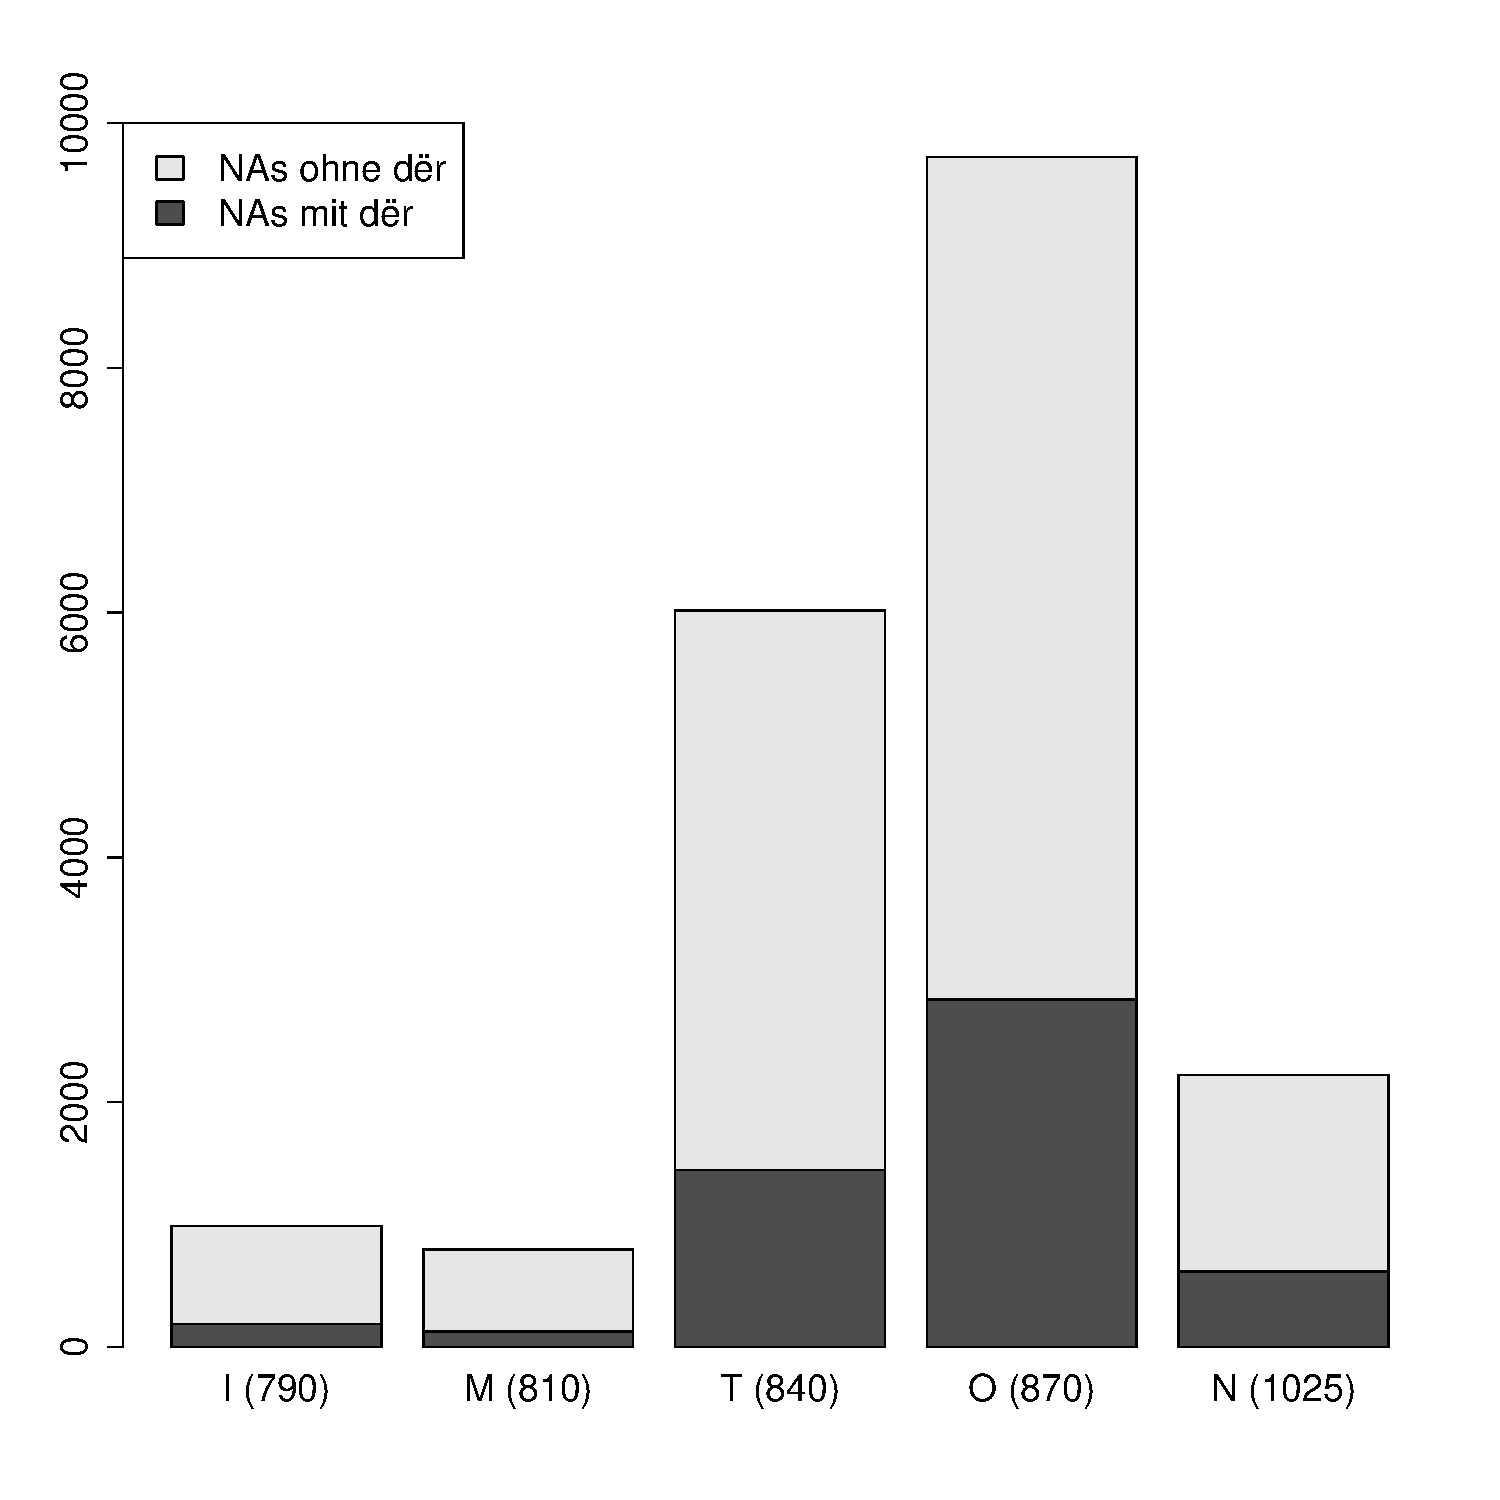
\includegraphics[width=\linewidth]{generated/images/artikel-anzahl-abs}
\caption {Absolute Zahlen}
\label{fig:art-abs}
\end{subfigure}%
\begin{subfigure}[b]{.5\linewidth}
  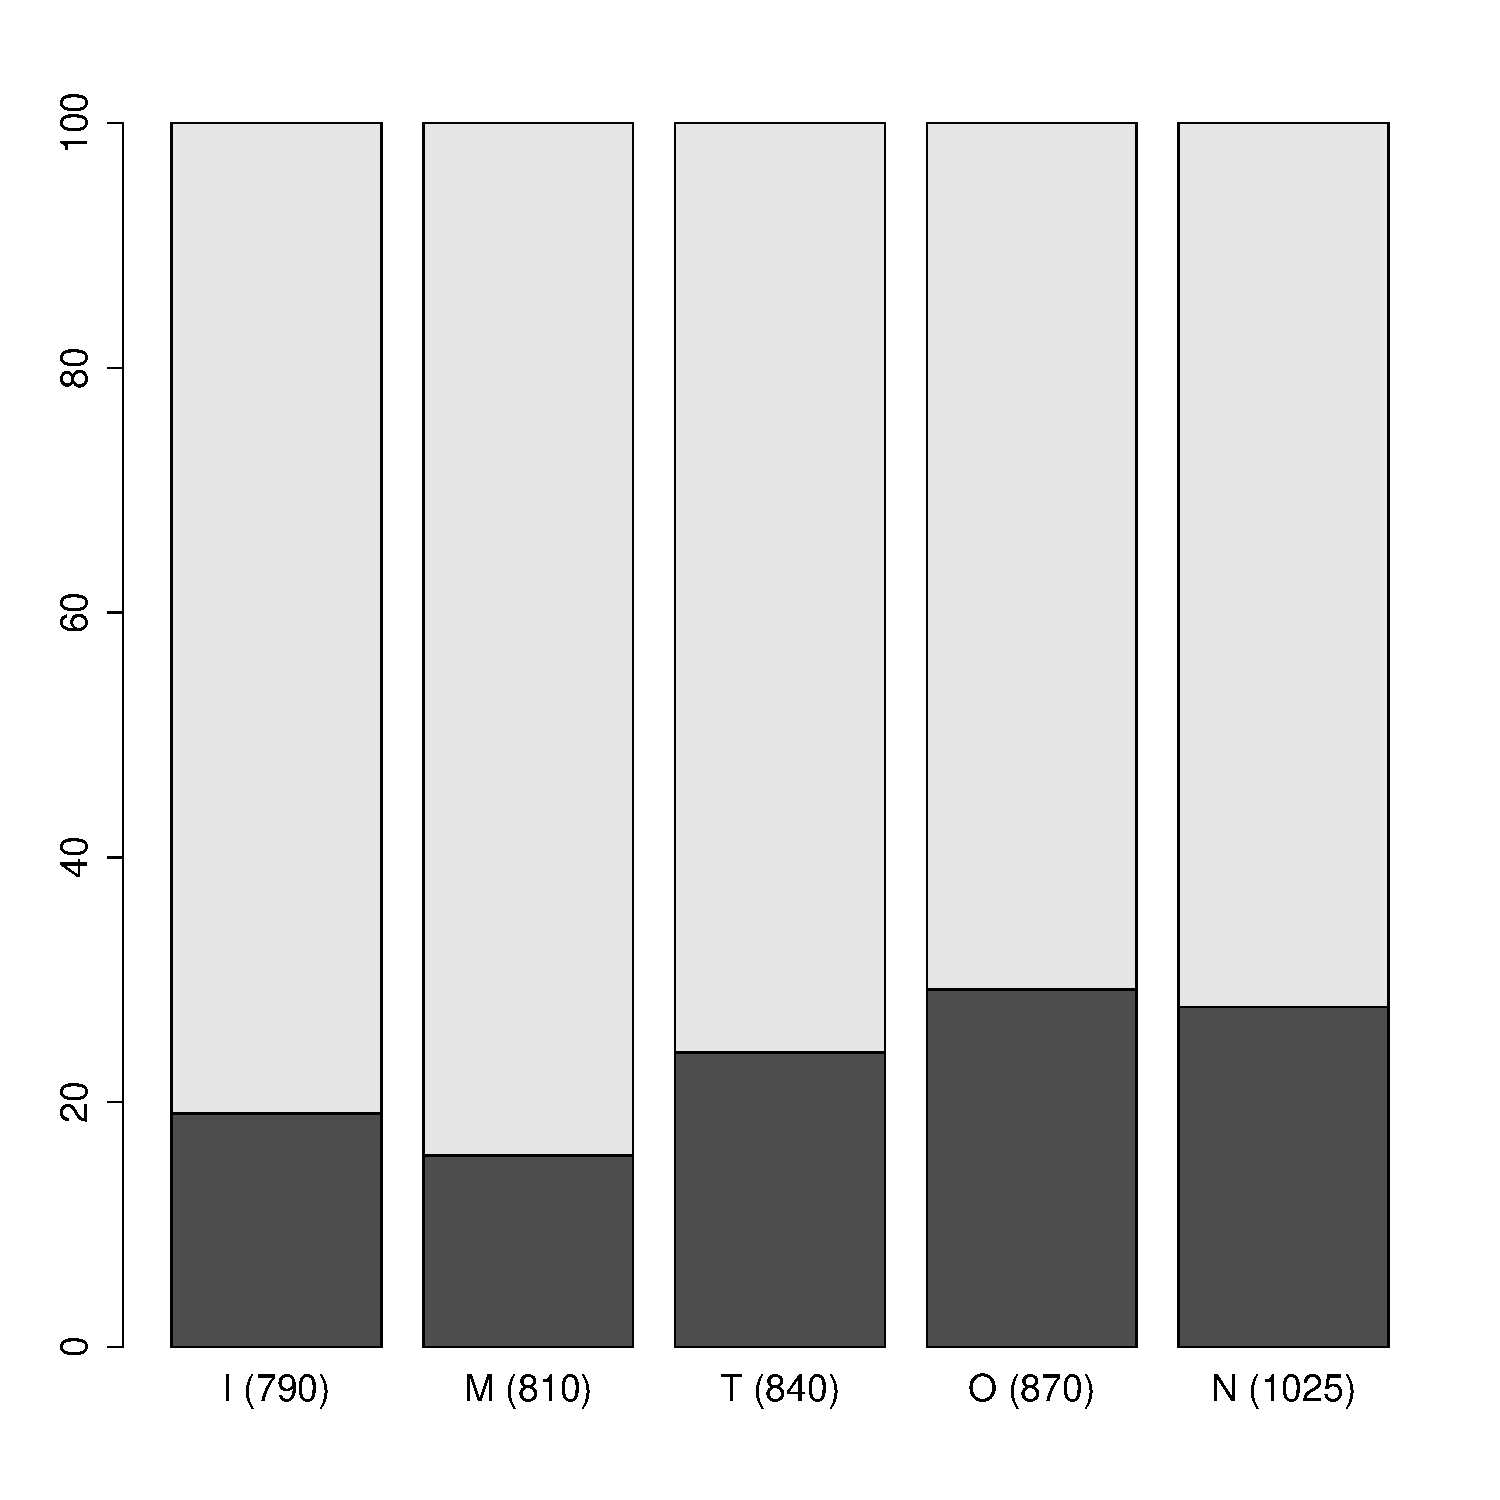
\includegraphics[width=\linewidth]{generated/images/artikel-anzahl-rel}
\caption {Relative Zahlen}
\label{fig:art-rel}
\end{subfigure}
\caption{Frequenz von \object{dër}}
\label{abb:art-freq}
\end{figure}
\vfill\pagebreak


Die relativen Zahlen auf der rechten Seite in Abbildung~\ref{abb:art-freq} verdeutlichen, dass \object{dër} immer mehr an Frequenz gewinnt.
Das älteste Denkmal (Isidor) sowie die jüngste Überlieferung (Notker) fallen allerdings aus der Reihe: Die Frequenzunterschiede zwischen Isidor und Monseer Matthäus sowie Otfrid und Notker sind jedoch nicht signifikant ($p > 0{,}05$, $\chi^2$-Test) und lassen sich vermutlich auf die Textsorte zurückführen. Wie schon in Abschnitt \ref{sec:textauswahl} erläutert, sind beim argumentativ ausgerichteten Isidor Bezüge auf zuvor genannte bzw. zentrale biblische Referenten häufig. Das Artikelwort \object{dër} kann helfen, diese Bezüge herzustellen. Doch wie die Ausführungen in \ref{sec:ergeb-defkontexte} zeigen werden, nutzt der Isidor-Übersetzer \object{dër} durchaus auch in semantischen Definitheitskontexten \is{Semantische Definita} und erweist sich dementsprechend als äußerst progressiv. Als einziger philosophischer Text enthält Notkers Boethius naturgemäß viele \is{Abstraktum} Abstrakta, die entsprechend lange undeterminiert bleiben und damit die \object{dër}-Frequenz nach unten drücken (vgl. hierzu Abschnitt \ref{sec:ergeb-faktoren}). 
Die Frequenzunterschiede zwischen den drei zeitlich dazwischen liegenden Schriftstücken sind hingegen hoch signifikant ($p < 0{,}001$, $\chi^2$-Test). Dabei sind der Monseer Matthäus, Tatian und Otfrid gut miteinander vergleichbar: Sie bestehen jeweils aus Erzählungen über die Taten Christi. Es scheint zudem, als würde auch das Reimschema \is{Reim} bei Otfrids Evangelienbuch (dem einzigen poetischen Text) dem Gebrauch von \object{dër} als Phraseneinleiter nicht entgegenstehen.  

\section{Das funktionale Spektrum von \object{dër}}\label{sec:ergeb-definitheit}

In Abschnitt \ref{sec:ergeb-defkontexte} werden die Ergebnisse der Stichprobenanalyse zu den Definitheitskontexten \is{Definitheitskontext} im Isidor, Tatian und bei Otfrid präsentiert. Anschließend fokussieren die Daten in Abschnitt \ref{sec:ergeb-superaltiv} und \ref{sec:ergeb-monosem} genuin abstrakt-definite Gebrauchskontexte, indem zunächst alle Superlativkonstruktionen \is{Superlativ} und dann ausgewählte Unika \is{Unikum} in den Texten betrachtet werden.  

\subsection{Definitheitskontexte}\label{sec:ergeb-defkontexte}

Pro Text wurde eine zufällige Stichprobe von 100 \isi{Token} mit dem PoS-Tag \hervor{NA} (Nomen Appellativum) \is{Gattungsname} ausgewählt und nach Definitheits- bzw. Indefinitheitskontexten \is{Indefinitheit}\is{Definitheitskontext}annotiert. Die nachfolgenden Werte entsprechen Nomen, die den Kern einer NP in Satzgliedfunktion bilden.\footnote{Die Stichprobe kann im R-Skript \hervor{aufbereitung.annotierte.daten} nachvollzogen werden. Dieses kann ebenso wie die annotierten Daten in \textcite{HZKYL4_2020} eingesehen werden.}   
Zentral für den funktionalen Wandel, ist die Frage, ob und in welchem Maße
[\object{dër}\,+\,N]-Phrasen \is{Phrase} gebraucht werden, um Referenten zu denotieren, die auch ohne explizite Vorerwähnung im Text oder im größeren Diskurskontext für den Adressaten identifizierbar sind, d.h. in den semantischen Definitheitskontexten \is{Semantische Definita} auftreten (vgl. Abschnitt \ref{sec:pragsem}). Ambige Fälle, die in allen Texten vorgekommen sind, werden später in Abschnitt \ref{sec:disk-bruecken} als mögliche Brückenkontexte \is{Brückenkontext} analysiert. 

%\subsubsection{Isidor} 

In der nachfolgenden Tabelle ist die Verteilung der 
100 annotierten NPs aus dem Isidor auf die unterschiedlichen Kontexttypen dargestellt. 16 der 100 NPs tragen ein \object{dër}.


\begin{table}
\centering
\begin{tabular}{llrrr}
\lsptoprule
{Definitheitsart}                                 & {Gebrauchskontexte}        & {mit \object{dër}} & {ohne \object{dër}} & {Summe} \\ \midrule
\multirow{4}{*}{Pragmatisch} & Situativ               & 0       & 0        & 0      \\
                                          & Anaphorisch            & 3       & 2        & 5      \\
                                          & Diskursdeiktisch       & 0       & 1        & 1      \\
                                          & Anamnestisch           & 2       & 0        & 2      \\ \midrule
\multirow{4}{*}{Semantisch}  & Abstrakt-situativ      & 7       & 25       & 32     \\
                                          & Assoziativ-anaphorisch & 0       & 1        & 1      \\
                                          & Monoreferenz                      & 1       & 17       & 18     \\
                                          & Generisch              & 1       & 6        & 7      \\ \midrule
\multirow{3}{*}{Nicht-definit}  & Nicht-spezifisch       & 0       & 11       & 11 \\
                                          & Spezifisch-indefinit   & 0       & 1        & 1      \\
                                          & Indefinit              & 0       & 6        & 6      \\ \midrule
\multirow{2}{*}{Andere Fälle}                   & mit Possessiva                    & 0       & 12       & 12     \\
                                          & Ambige Fälle                      & 2       & 2        & 4      \\ \midrule
\multicolumn{2}{c}{Summe}                                                    & 16      & 84       & 100    \\ \lspbottomrule
\end{tabular}
\caption{Definitheits- und Indefinitheitskontexte \is{Indefinitheit}\is{Definitheitskontext}im Isidor}
\label{tab:definitheit-I}
\end{table}
%basierend auf: Stichprobe.Definitheit.R
%\inputtable{generated/tables/definitheit-I}{Definitheitskontexte im Isidor}{tab:definitheit-I}

Erwartet wurde, dass in diesem frühen ahd. Text vor allem Referenten mit [\object{dër}\,+\,N]-Phrasen \is{Phrase} denotiert werden, die durch den unmittelbaren Text oder einen vorherigen Diskurs vorerwähnt sind und dadurch identifizierbar wurden \is{Pragmatische Definita} (=\,prag\-ma\-tische Gebrauchskontexte). Daher überrascht es, dass nur fünf der 16 Phrasen diesem Definitheitstypus entsprechen (3 $\times$ anaphorisch \is{anaphorisch} und 2 \is{anamnestisch} $\times$ anamnestisch). In Beispiel \REF{ex:I1051} ist ein Beleg für den  anaphorischen Gebrauch \is{anaphorisch} aufgeführt. Mit \object{dher aerlose man} wird auf einen  zuvor erwähnten König Bezug genommen.  

% Basis:
%\begin{exe}
\ex \label{ex:I1051} \gll \object{Ibu} \object{dhanne} \object{einic} \object{chilaubit} \object{0} \object{dhazs} \object{dhiz} \object{fona} \object{cyre} \object{persero} \object{chuninge} \object{sii} \object{chiforabodot} \object{0} \object{bichnaa} \object{sih} \object{dher} \object{0} \object{dhazs} \object{izs} \object{uuidharzuomi} \object{endi} \object{heidhanliih} \object{ist} \object{eomanne} \object{zi} \object{chilaubanne} \object{0} \object{dhazs} \object{dher} \object{aerloso} \object{\underline{man}} \object{endi} \object{dher} \object{heidheno} \object{abgudim} \object{gheldendo} \object{christ} \object{0} \object{got} \object{endi} \object{druhtin} \object{uurdi} \object{chinemnit} \object{. } \\
{wenn} {dann} {irgendein} {glauben} {} {dass} {dieser} {von} {Kyrus} {Perser} {König} {sein} {ankündigen} {} {klarmachen} {sich} {der} {} {dass} {er} {widersinnig} {und} {heidnisch} {sein} {(irgend)jemand} {zu} {glauben} {} {dass} {der} {gottlos} {Mann} {und} {der} {Heide} {Götzen(bilder)} {geben} {Christus} {} {Gott} {und} {Herr} {werden} {nennen} {}\\
\glt TODO: nhd. Übersetzung (I.3,3)
\end{exe}


\begin{exe}
\ex \label{ex:I1051} \gll  dhazs dhiz fona cyre persero chuninge dhazs \textit{dher} \textit{aerloso} \textit{man} \\
{dass} {dieser} {von} {Kyrus} {Perser} {König} {dass} {dieser} {gottlose} {Mann} \\
\glt   \extrans{dass dieser Perserkönig von Kyrus dass  dieser gottlose Mann} (I 3,3)
\end{exe}

Der Beleg in \REF{ex:I2524} ist exemplarisch für den anamnestischen \is{anamnestisch} Gebrauch. Für die \isi{Phrase} \object{dhurach dhen selbun heilegun forasagun} gibt es keinen unmittelbar vorerwähnten Antezedens. Trotzdem kann man davon ausgehen, dass die Leserschaft weiß, dass es sich um den Propheten handelt, der schon in einigen Abschnitten vorher erwähnt wurde.
%Basis
%\begin{exe}
\ex \label{ex:I2524} \gll \object{So} \object{auh} \object{in} \object{andreru} \object{stedi} \object{dhurah} \object{dhen} \object{selbun} \object{heilegun} \object{\underline{forasagun}} \object{uuard} \object{dhera} \object{dhrinissa} \object{bauhnunc} \object{sus} \object{araughit} \object{: } \\
{so} {auch} {in} {anderer} {Stätte} {durch} {der} {selber} {heilig} {Prophet} {werden} {der} {Dreiheit} {Bezeichnung} {so} {offenbaren} {}\\
\glt TODO: nhd. Übersetzung (I.4,8)
\end{exe}


\begin{exe}
\ex \label{ex:I2524} \gll So auh in andreru stedi \textit{dhurah} \textit{dhen} \textit{selbun} \textit{heilegun} \textit{forasagun} uuard dhera dhrinissa bauhnunc sus araughit  \\
{so} {auch} {in} {anderer} {Stelle} {durch} {den} {selben} {heiligen} {Propheten} {ward} {der} {Dreifaltigkeit} {Bezeichnung} {so} {offenbart} \\
\glt   \extrans{Auch an andere Stelle wird durch diesen selben heiligen Propheten die Bezeichnung der Dreifaltigkeit offenbart.} (I 4,8)
\end{exe}

Mit den restlichen [\object{dër}\,+\,N]-Belegen werden Referenten denotiert, die auch ohne den Kontext eindeutig identifizierbar sind. In einem Fall liegt Monoreferenz vor. Die \object{dër}-\isi{Phrase} ist in eine indirekte Frage eingebettet: \object{huueo dher sunu mahti fona fater chiboran uuerdhan} \extrans{wie der Sohn vom Vater (Gott) geboren werden konnte} (I 2,3). 

In \REF{ex:I683} ist ein Beispiel für den abstrakt-situativen \is{abstrakt-situativ} Gebrauch. 
%Basis
%\begin{exe}
\ex \label{ex:I683} \gll \object{Christus} \object{auur} \object{sus} \object{quham} \object{fona} \object{fater} \object{ziuuaare} \object{so selp so} \object{dhiu} \object{\underline{berahtnissi}} \object{fona} \object{sunnun} \object{0} \object{so} \object{uuort} \object{fona} \object{munde} \object{0} \object{so} \object{uuiisduom} \object{fona} \object{herzin} \object{. } \\
{Christus} {aber} {so} {kommen} {von} {Vater} {gewiss} {ebenso wie} {der} {Ehre} {von} {Sonne} {} {so} {Wort} {von} {Mund} {} {so} {Weisheit} {von} {Herz} {}\\
\glt TODO: nhd. Übersetzung (I.2,5)
\end{exe}

\begin{exe}
\ex \label{ex:I683} \gll {Christus} {auur} {sus} {quham} {fona} {fater} {ziuuaare} {so selp so} {\textit{dhiu}} {\textit{berahtnissi}} {fona} {sunnun}, {so} {uuort} {fona} {munde}, {so} {uuiisduom} {fona} {herzin} \\
{Christus} {aber} {so} {kam} {von} {Vater} {gewiss} {ebenso wie} {der} {Glanz} {von} {Sonne}, {so} {Wort} {von} {Mund}, {so} {Weisheit} {von} {Herz} {}\\
\glt \extrans{Christus aber kam gewiss vom Vater genauso wie der Glanz von der Sonne, wie das Wort vom Mund, die Weisheit vom Herz} (I 2,5)
\end{exe}

Interessanterweise konnte ein \object{dër}-Beleg auch als generisch \is{generisch} klassifiziert werden, s. \REF{ex:I4768}. Mit \object{dhea iudea} wird eine allgemeine Charakterisierung über die Juden vorgenommen. 
%Basis:
%\begin{exe}
\ex \label{ex:I4768} \gll \object{Dhea} \object{\underline{iudea}} \object{auur} \object{dhurah} \object{iro} \object{grimmin} \object{mit} \object{dhemu} \object{unscama} \object{habendin} \object{andine} \object{quhedhant} \object{leogando} \object{dhazs} \object{noh} \object{ni} \object{sii} \object{dhazs} \object{ziidh} \object{arfullit} \object{0} \object{ni} \object{uueizs} \object{ih} \object{einigan} \object{chuninc} \object{fona} \object{iudases} \object{edhile} \object{noh} \object{in} \object{uzssonondem} \object{endum} \object{oostarriihhes} \object{uualdendan} \object{. } \\
{der} {Juden} {aber} {durch} {er} {Grimm} {mit} {der} {Schamlosigkeit} {haben} {Stirn} {sprechen} {lügen} {dass} {noch} {nicht} {sein} {der} {Zeit} {erfüllen} {} {nicht} {wissen} {ich} {irgendein} {König} {von} {Judas} {Adel} {noch} {in} {äußerst} {Ende} {Ost(franken)reich} {walten} {}\\
\glt TODO: nhd. Übersetzung (I.8,2)
\end{exe}


\begin{exe}
\ex \label{ex:I4768} \gll {\textit{Dhea}} {\textit{iudea}} {auur} {dhurah} {iro} {grimmin} {mit} {der} {unscama} {habendin} {andine} {quhedhant} {leogando} {dhazs}\\
{der} {Juden} {aber} {durch} {ihren} {Ingrimm} {mit} {der} {Schamlosigkeit} {haben} {Stirn} {sprechen} {lügend} {dass}\\
\glt \extrans{Aber die Juden sagen durch ihren Ingrimm mit Schamlosigkeit lügend, dass}(I 8,2)
\end{exe}

In allen 16 Fällen erfolgt die \object{dër}-Setzung entgegen der Vorlage, so dass lateinischen Interferenzen ausgeschlossen werden können. Zu den nicht-spezifischen Referenten \is{Spezifizität} gehören adverbiale \is{Adverbial} Angaben wie \object{duruh riuwa} \extrans{durch Reue}(I 5,10) oder Nomen in Funktionsverbefügen wie \object{man wërdan} \extrans{Mensch werden} (I 5,1). Der eine spezifisch-indefinite \is{Spezifizität} Beleg bezieht sich auf die \isi{Phrase} \object{mit sumes chirunes uuagu} \extrans{mit einer gewissen Waage} (I 4,9). In der Gruppe \hervor{indefinite Referenten} addieren sich Belege mit weniger salienten und unspezifischen \is{Spezifizität} Referenten wie \object{oba drato
hoh hohsedal} \extrans{auf einem hohen Thron} (I 4,10). Die Gruppe \hervor{mit Possessiva} \is{Possessivum}enthält \is{Phrase} Phrasen, die durch einen \is{Possessivum} Possessivartikel eingeleitet werden. 

%\subsubsection{Tatian} 

Im Vergleich zum Isidor nehmen im Tatian die semantisch-definiten Kontexte \is{Semantische Definita} mehr Raum ein. Wie in Tabelle~\ref{tab:definitheit-T} zu sehen ist, enthalten knapp ein Drittel (11 von 35 Belege) der abstrakt-situativen \is{abstrakt-situativ} Gebrauchskontexte ein \object{dër}.

\begin{table}
\centering
\begin{tabular}{llrrr}
\lsptoprule
{Definitheitsart}                                 & {Gebrauchskontext}        & {mit \object{dër}} & {ohne \object{dër}} & {Summe} \\ \midrule
\multirow{4}{*}{Pragmatisch} & Situativ               & 0       & 1        & 1      \\
                                          & Anaphorisch            & 1       & 3        & 4      \\
                                          & Diskursdeiktisch       & 0       & 1        & 1      \\
                                          & Anamnestisch           & 1       & 0        & 1      \\ \midrule
\multirow{4}{*}{Semantisch}  & Abstrakt-situativ      & 11       & 24       & 35 \\
                                          & Assoziativ-anaphorisch & 2       & 1        & 3      \\
                                          & Monoreferenz                      & 10       & 1       & 11     \\
                                          & Generisch              & 0       & 4        & 4      \\ \midrule
\multirow{3}{*}{Nicht-definit}  & Nicht-spezifisch       & 0       & 10       & 10     \\
                                          & Spezifisch-indefinit   & 0       & 2        & 2      \\
                                          & Indefinit              & 0       & 9        & 9      \\ \midrule
\multirow{2}{*}{Andere Fälle}                   & mit Possessiva                    & 0       & 14       & 14     \\
                                          & Ambige Fälle                      & 2       & 3        & 5      \\ \midrule
\multicolumn{2}{c}{Summe}                                                    & 27      & 73       & 100    \\ \lspbottomrule
\end{tabular}
\caption{Definitheits- und Indefinitheitskontexte \is{Indefinitheit}\is{Definitheitskontext}im Tatian}
\label{tab:definitheit-T}
\end{table}

%%basierend auf:
%\inputtable{generated/tables/definitheit-T}{Definitheitskontexte im Tatian}{tab:definitheit-T}

 Die Fälle von Monoreferenz mit \object{dër} beziehen sich immer auf \object{Jesus}; 8 Mal steht es in Kombination mit \object{heilant}, ansonsten mit \object{sun}. Zudem finden sich unter den insgesamt 27 \object{dër}-Phrasen \is{Phrase} auch zwei assoziativ-anaphorische \is{assoziativ-anaphorisch} Kontexte, s. hierfür exemplarisch der Beleg in \REF{ex:T27561}. 

% Basis 
%\begin{exe}
\ex \label{ex:T27561} \gll \object{Maria} \object{habenti} \object{salbfaz} \object{salbun} \object{fon} \object{narthu} \object{gitana} \object{diura} \object{0} \object{inti} \object{gibrohanemo} \object{goz} \object{ubar} \object{sin} \object{houbit} \object{linentes} \object{0} \object{inti} \object{salbota} \object{sine} \object{fuozi} \object{inti} \object{suarb} \object{mit} \object{ira} \object{locon} \object{0} \object{inti} \object{thaz} \object{hus} \object{uuas} \object{gifullit} \object{fon} \object{themo} \object{\underline{stanke}} \object{thera} \object{salbun} \object{.} \\
{Maria} {haben} {Salbgefäß} {Salbe} {von} {Narde(nöl)} {tun} {teuer} {} {und} {(ab)brechen} {(ver)gießen} {über} {sein} {Haupt} {niedersinken} {} {und} {(ein)salben} {sein (eigen)} {Fuß} {und} {abreiben} {mit} {er} {Locke} {} {und} {dieser} {Haus} {sein} {(er)füllen} {von} {dieser} {(Wohl)geruch} {dieser} {Salbe} {}\\
\glt TODO: nhd. Übersetzung (T.138,1)
\end{exe}


\begin{exe}
\ex \label{ex:T27561} \gll {inti} {salbota} {sine} {fuozi} {inti} {suarb} {mit} {ira} {locon}, {inti} {thaz} {hus} {uuas} {gifullit} {fon} {\textit{themo}} {\textit{stanke}} {thera} {salbun}  \\
{und} {salbte} {seinen } {Fuß} {und} {rieb} {mit} {ihren} {Locken}, {und} {das} {Haus} {war} {erfüllt} {von} {dem} {Geruch} {der} {Salbe} \\
\glt \extrans{Und sie salbte seine Füße und trocknete sie mit ihren Haaren ab und das Haus war mit dem Geruch der Salbe gefüllt} (T 138,1)
\end{exe}

Generische Phrasen mit \object{dër} waren in der Stichprobe nicht dabei. Die Untersuchung von \textcite{Oubouzar1989,Oubouzar1992} hat allerdings gezeigt, dass diese im Tatian durchaus vorhanden sind (vgl. auch Abschnitt \ref{sec:pragsem}). Alle \object{dër}-Setzungen sind \is{Differenzbeleg} Differenzbelege, d.h. in der lateinischen Vorlage gibt es keine \isi{Demonstrativartikel} als Äquivalent.

%\subsubsection{Otfrid} 

Tabelle~\ref{tab:definitheit-O} zeigt die Verteilung der definiten bzw. indefiniten Gebrauchskontexte auf die 100 NPs bei Otfrid. Fast die Hälfte aller abstrakt-situativen \is{abstrakt-situativ} Gebrauchskontexte (18 von 37 Belege) werden hier mithilfe von \object{dër}-Phrasen \is{Phrase} zum Ausdruck gebracht.

\begin{table}
\centering
\begin{tabular}{llrrr}
\lsptoprule
{Definitheitsart}                                 & {Gebrauchskontext}        & {mit \object{dër}} & {ohne \object{dër}} & {Summe} \\ \midrule
\multirow{4}{*}{Pragmatisch} & Situativ               & 0                & 1                 & 1 \\
                                          & Anaphorisch            & 1                & 1 & 2               \\
                                          & Diskursdeiktisch       & 0                & 1                 & 1               \\
                                          & Anamnestisch           & 0                & 0                 & 0               \\  \midrule
\multirow{4}{*}{Semantisch}  & Abstrakt-situativ      & 18                & 19 & 37              \\
                                          & Assoziativ-anaphorisch & 0                & 0                 & 0               \\
                                          & Monoreferenz                      & 0                & 5                & 5              \\
                                          & Generisch              & 2                & 2                 & 4               \\  \midrule
\multirow{3}{*}{Nicht-definit}  & Nicht-spezifisch       & 0                & 22                & 22              \\
                                          & Spezifisch-indefinit   & 0                & 1                 & 1               \\
                                          & Indefinit              & 0                & 11                 & 11               \\  \midrule
\multirow{2}{*}{Andere Fälle}                   & mit Possessiva                    & 1                & 11                & 12              \\
                                          & Ambige Fälle                      & 2                & 2                 & 4               \\  \midrule
\multicolumn{2}{c}{Summe}                                                    & 24               & 76                & 100             \\ \lspbottomrule
\end{tabular}
\caption{Definitheits- und Indefinitheitskontexte \is{Indefinitheit}\is{Definitheitskontext}bei Otfrid}
\label{tab:definitheit-O}
\end{table}\pagebreak

% basierend auf\inputtable{generated/tables/definitheit-O}{Definitheitskontexte im Otfrid}{tab:definitheit-O}

Fälle von assoziativ-anaphorischer \is{assoziativ-anaphorisch} Definitheit sind in der Stichprobe nicht belegt. Generische Ausdrücke kommen gleich häufig mit (vgl. \ref{ex:O62652}) und ohne (vgl. \ref{ex:O72468}) \object{dër} vor.

% Basis:
%\begin{exe}
\ex \label{ex:O62652} \gll \object{Ther} \object{\underline{mán}} \object{ther} \object{thaz} \object{súachit} \object{thes} \object{er} \object{hárto} \object{ruachit} \object{:} \\
{der} {Mensch; Mann} {der} {der} {suchen} {der} {er} {sehr} {sich sehnen} {}\\
\glt TODO: nhd. Übersetzung (O.5,7)
\end{exe}


\begin{exe}
\ex \label{ex:O62652} \gll {\textit{Ther}} {\textit{mán}} {ther} {thaz} {súachit} {thes} {er} {hárto} {ruachit} \\
{der} {Mensch} {der} {das} {sucht} {dessen} {er} {sehr} {sich sehnt} \\
\glt   \extrans{Der Mensch, der das sucht, wonach er sich sehr sehnt} (O V,7)
% Basis
%\begin{exe}
\ex \label{ex:O72468} \gll \object{Hiar} \object{síudit} \object{\underline{mánne}} \object{ana} \object{wánk} \object{io} \object{ther} \object{úbilo} \object{githánk} \object{in} \object{hérzen} \object{joh} \object{in} \object{múate} \object{0} \object{ni} \object{firséhent} \object{sih} \object{zi} \object{gúate} \object{;} \\
{hier} {brennen} {Mensch; Mann} {ohne} {Zweifel} {immer} {der} {übel} {Gedanke; Gesinnung} {in} {Herz} {und} {in} {Sinn} {} {nicht} {schauen} {sich} {zu } {Gutes} {}\\
\glt TODO: nhd. Übersetzung (O.5,23)
\end{exe}


\ex \label{ex:O72468} \gll {Hiar} {síudit} {\textit{mánne}} {ana} {wánk} {io} {ther} {úbilo} {githánk} {in} {hérzen} {joh} {in} {múate}  \\
{hier} {brennt} {(dem) Menschen} {ohne} {Zweifel} {immer} {der} {übel} {Gedanke} {in} {Herz} {und} {in} {Gemüt} \\
\glt   \extrans{Hier brennt dem Menschen zweifellos der üble Gedanke im Herzen und im Gemüt}  (O V,23)
\end{exe}

Die Anzahl der \object{dër}-Phrasen \is{Phrase} im Bereich der semantischen Definita \is{Semantische Definita} ist bei Otfrid im Vergleich zu den beiden älteren Texten also größer. In den pragmatischen Definitheitskontexte \is{Pragmatische Definita} findet sich hingegen nur ein Beleg mit \object{dër}, und zwar im Rahmen eines anaphorischen \is{anaphorisch} Kontexts. Der eine Beleg für den diskursdeiktischen \is{diskursdeiktisch} Bezug wird mit \object{dëser} \is{Demonstrativum}eingeleitet (\object{in thésera noti} \extrans{in dieser Not(lage))}; O III 20), ebenso wie der Beleg mit situativer Referenz \is{situativ} \object{these kísila} \extrans{dieser Kieselstein} (O I,23) sowie der zweite anaphorische \is{anaphorisch} Beleg. Die Ergebnisse sprechen dafür, dass sich [\object{dër}\,+\,N] als Ausdruck für semantische Definitheitskontexte \is{Semantische Definita} etabliert hat. Die Setzung ist allerdings nicht obligatorisch. Die Struktur [\object{dëser}\,+\,N] scheint sich hingegen auf pragmatische Definita \is{Pragmatische Definita} spezialisiert zu haben; bei den semantischen Definita \is{Semantische Definita} kommt sie nicht vor.

\subsection{Superlative}\label{sec:ergeb-superaltiv}

Superlative \is{Superlativ} sind Indikatoren für semantisch-definite \is{Semantische Definita} Gebrauchskontexte  (vgl.\linebreak Abschnitt \ref{sec:nicht-fam}), da unabhängig von der Äußerungssituation  immer nur ein Referent in Frage kommt, der als \object{die beste Schauspielerin} oder \object{das Schönste} ausgezeichnet werden kann. Sprachen mit \isi{Definitartikel} setzen in diesen Kontexten immer einen \isi{Definitartikel} \parencite{Himmelmann2001}. Der Austausch mit einem \isi{Demonstrativum} ist hier nicht möglich. Denn es geht bei dieser Artikelsetzung nicht darum, einen bestimmten Referenten (in Abgrenzung zu anderen potentiellen Referenten) identifizierbar zu \hervor{machen}, sondern die definite Lesart lediglich als solche zu markieren \parencite[41]{Himmelmann1997}.

In Tabelle~\ref{tab:superlative} werden die Häufigkeiten der attributiven Adjektive \is{Adjektiv} im \isi{Superlativ} mit und ohne \object{dër} miteinander verglichen. Tabelle~\ref{tab:subst:superlative} zeigt, wie viele substantivierte \is{Substantivierung} Superlative \is{Superlativ} mit \object{dër} determiniert werden. In beiden Fällen wurde ein Beleg genau dann als mit \object{dër} determiniert gezählt, wenn dem \isi{Superlativ} ein \isi{Token} mit dem PoS-Tag \hervor{DDA} unmittelbar vorausgeht und mit diesen in \isi{Kasus}, \isi{Genus} und \isi{Numerus} übereinstimmt. 

Man sieht, dass der Strukturtyp \is{Superlativ}\is{Adjektiv}[\object{dër}\,+\,Adjektiv\textsubscript{Superlativ}\,+\,N] in allen Texten deutlich häufiger vorkommt als der Strukturtyp [Adjektiv\textsubscript{Superlativ}\,+\,N]. Bei den substantivierten Adjektiven \is{Substantivierung}\is{Adjektiv}gibt es hingegen nur im Tatian und bei Notker mehr Belege mit \object{dër} als ohne. Die wichtigste Beobachtung aus den Daten in Tabelle~\ref{tab:subst:superlative} ist, dass in allen Texten die Struktur \object{dër}\,+\,substantivierter \is{Substantivierung} \isi{Superlativ} belegt und damit grundsätzlich auch schon im frühen Althochdeutschen möglich ist. 

%basierend auf "Adjektive.R"
%\object{dër}-Setzung bei Superlativen: [(\object{dër}\,+\,) Ad\-jek\-tiv\textsubscript{Superlativ}\,+\,N)]
 
 
\begin{table}
\begin{tabular}{lrr}
\lsptoprule
              {Text}         & {mit \object{dër}} & {ohne \object{dër}} \\ \midrule
Isidor (790)           & 2                              & 0                           \\
Monseer Matthäus (810) & 4                              & 1                           \\
Tatian (840)           & 20                             & 7 \\
Otfrid (870)           & 7                            & 5                          \\
Notker (1025)          & 9                             & 1                           \\ \lspbottomrule
\end{tabular}
\caption{Strukturtypen im Vergleich: [\object{dër}\,+ Ad\-jek\-tiv\textsubscript{Superlativ}\,+\,N] vs. [Ad\-jek\-tiv\textsubscript{Superlativ}\,+\,N]}
\label{tab:superlative}
\end{table}

\begin{table}
\begin{tabular}{lrr}
\lsptoprule
              {Text}         & {mit \object{dër}} & {ohne \object{dër}} \\ \midrule
Isidor (790)           & 4                              & 6                           \\
Monseer Matthäus (810) & 3                              & 8                           \\
Tatian (840)           & 26                             & 13 \\
Otfrid (870)           & 2                            & 16                          \\
Notker (1025)          & 15                             & 3                           \\ \lspbottomrule
\end{tabular}
\caption{\object{dër}-Setzung bei substantivierten Superlativen}
\label{tab:subst:superlative}
\end{table}

\subsection{Unika} \label{sec:ergeb-monosem}

Unika \is{Unikum} referieren genau auf einen, im Diskursuniversum bekannten Referenten. Der Gebrauch eines demonstrativen \is{Demonstrativartikel} Artikelwortes, das der Referenzfindung bzw. -abgrenzung \is{Referentialität} dient, ist bei diesen Substantivtypen \is{Substantiv} überflüssig. Tritt ein \object{dër} bei Unika \is{Unikum} auf, ist dies daher ein gutes Indiz dafür, dass der funktionale Wandel Richtung \isi{Definitartikel} im Vollzug ist und das Muster [\object{dër}\,+\,N] sich auch auf semantisch-definite Kontexte \is{Semantische Definita} ausbreitet. Auf Basis der Studien von  \textcite{Graf1905}, \textcite{Bell1907}, \textcite{Hodler1954}, \textcite{Oubouzar1989} sowie der Fallstudie von \textcite[75]{Szczepaniak2011a} wurden Lemmata \is{Lemma} ausgewählt, die auf einzigartige und der ahd. Leserschaft bekannte Referenten verweisen: 

\begin{itemize}
\item Einmalige Referenten in der Natur\\
\object{sunna} \extrans{Sonne}, \object{mano} \extrans{Mond}, \object{himil} \extrans{Himmel}, \object{ërda} \extrans{Erde}, \object{wëralt} \extrans{Welt}
\item Unika aus dem christlichen Kulturkreis:\\
\object{heilant} \extrans{Jesus}, \object{geist} \extrans{(der heilige) Geist}, \object{got} \extrans{Gott},  \object{tiufal} \extrans{Teufel}
\end{itemize}

\noindent 
Die nachfolgenden Tabellen dokumentieren, ob \isi{Token} dieser Lemmata \is{Lemma} mit einem kongruierenden \object{dër} auftreten. Genau wie in Abschnitt \ref{sec:ergeb-ther-freq}  wurde hierfür für die Suche das gesamte \isi{Korpus} als Grundlage genommen und sowohl Fälle mit unmittelbarer Determination (\object{dër}\,+\,N) als auch Belege mit Distanzstellung (\object{dër}\,+\,X\,+\,N) einbezogen.
% Tabellen auf Basis von "lemma.R" 

Bei \object{sunna} und \object{mano} zeigt sich, dass in den frühen Schriftstücken keine Determination mit \object{dër} stattfindet, s. Tabellen~\ref{tab:sonne} und \ref{tab:mond}. 

\begin{table}
\begin{tabular}{lrr}
\lsptoprule
{Text}  & {mit \object{dër}} & {ohne \object{dër}} \\ \midrule
Isidor (790)           & 0                & 2                   \\
Monseer Matthäus (810) & 0                & 3                   \\
Tatian (840)           & 1                & 3                   \\
Otfrid (870)           & 4                & 15                  \\
Notker (1025)          & 10               & 7                   \\ \lspbottomrule
\end{tabular}
\caption{\object{dër}-Setzung bei \object{sunna} \extrans{Sonne}}
\label{tab:sonne}
\end{table}

\begin{table}
\begin{tabular}{lrr}
\lsptoprule
{Text}  & {mit \object{dër}} & {ohne \object{dër}}  \\ \midrule
Isidor (790)           & 0           & 1              \\
Monseer Matthäus (810) & 0           & 1              \\
Tatian (840)           & 0           & 2              \\
Otfrid (870)           & 1           & 3              \\
Notker (1025)          & 3           & 0              \\ \lspbottomrule
\end{tabular}
\caption{\object{dër}-Setzung bei \object{mano} \extrans{Mond}}
\label{tab:mond}
\end{table}

Im Tatian gibt es bei \object{sunna} genau einen Beleg mit \object{dër}, s. \REF{ex:T6760}. Interessanterweise steht, wie auch \textcite[20]{Graf1905} beobachtet, in der lateinischen Vorlage ein \isi{Possessivum}: \object{quia solem suum oriri facit}. Dies könnte laut \textcite[216]{Oubouzar1989} ein Beleg für die funktionale Überschneidung von \object{dër} mit determinierenden \is{Determinierer}\is{Possessivum}Possessiva sein.

%Basiert auf: 
%\begin{exe}
\ex \label{ex:T6760} \gll \object{Thaz} \object{ír} \object{sít} \object{kind} \object{íuuares} \object{fater} \object{thie} \object{in} \object{himile} \object{ist} \object{0} \object{ther} \object{thie} \object{\underline{sunnun}} \object{úf} \object{gangen} \object{tuot} \object{ubar} \object{ubile} \object{inti} \object{ubar} \object{guote} \object{inti} \object{reganot} \object{ubar} \object{rehte} \object{inti} \object{ubar} \object{únrehte} \object{.} \\
{daß} {ihr} {sein} {Kind} {euer} {Vater} {der} {in} {Himmel} {sein} {} {der} {der} {Sonne} {auf} {aufgehen} {tun} {über} {Übel} {und} {über} {Gute} {und} {regnen} {über} {Recht} {und} {über} {Unrecht} {}\\
\glt TODO: nhd. Übersetzung (T.32,3)
\end{exe}


\begin{exe}
\ex \label{ex:T6760} \gll {ther} {\textit{thie}} {\textit{sunnun}} {úf} {gangen} {tuot} \\
{der} {die} {Sonne} {auf} {gehen} {tut}  \\
\glt   \extrans{[Gott] der die Sonne aufgehen lässt} (T 32,3)
\end{exe}

Der erste Nachweis von \object{dër}\,+\,\object{mano} findet sich in Otfrids Evangelienbuch und zwar in einer Paarformel in Verbindung mit \object{sunna}, s. \REF{ex:O68453}.
%  basiert auf: 
%\begin{exe}
\ex \label{ex:O68453} \gll \object{Thia} \object{súnnun} \object{joh} \object{then} \object{\underline{mánon}} \object{so} \object{úbar} \object{fuar} \object{er} \object{gáhon} \object{0} \object{joh} \object{állan} \object{thesan} \object{wóroltring} \object{0} \object{ni} \object{gisah} \object{man} \object{ér} \object{io} \object{sulih} \object{thíng} \object{;} \\
{der} {Sonne} {und} {der} {Mond} {so} {über} {hinweggehen (über)} {er} {schnell} {} {und} {all} {dieser} {Erdkreis} {} {nicht} {sehen} {Mensch; Mann} {eher} {jemals} {solch} {Ding} {}\\
\glt TODO: nhd. Übersetzung (O.5,17)
\end{exe}

\begin{exe}
\ex \label{ex:O68453} \gll {\textit{Thia}} {\textit{súnnun}} {joh} {\textit{then}} {\textit{mánon}} {so} {úbar} {fuar} {er} {gáhon}  \\
{die} {Sonne} {und} {den} {Mond} {so} {über} {fährt} {er} {schnell} \\
\glt   \extrans{So überschreitet er die Sonne und den Mond schnell} (O V,17)
\end{exe}
\noindent 
Hier könnte die Setzung von \object{dër} auch metrisch \is{Metrik} bedingt sein \parencite[20]{Graf1905}. Dennoch kann man davon ausgehen, dass alleine die Möglichkeit, ein \object{dër} mit \object{mano} zu kombinieren, eine Abschwächung der demonstrativen Funktion voraussetzt. Erst bei Notker überwiegen sowohl bei \object{sunna} als auch bei \object{mano} die determinierten Belege, was auf eine  Koventionalisierung von [\object{dër}\,+\,N] hindeutet. Zur Illustration ist nachfolgend ein Beispiel aufgeführt, das sowohl [\object{dër}\,+\,\object{mano}] als auch [\object{dër}\,+\,\object{sunna}] enthält. 
%basiert auf:
%\begin{exe}
\ex \label{ex:N8884} \gll \object{dáz_} \object{ter} \object{mâno} \object{uuîlon} \object{fóllêr} \object{gâendo} \object{gágen} \object{dero} \object{\underline{súnnûn}} \object{. } \\
{dass} {der} {Mond} {bisweilen} {voll} {gehen} {gegen} {der} {Sonne} {}\\
\glt TODO: nhd. Übersetzung (N.1,31)
\end{exe}


\begin{exe}
\ex \label{ex:N8884} \gll {dáz} {\textit{ter}} {\textit{mâno}} {uuîlon} {fóllêr} {gâendo} {gágen} {\textit{dero}} {\textit{súnnûn}}  \\
{dass} {der} {Mond} {bisweilen} {voller} {gehend} {gegen} {der} {Sonne}\\
\glt   \extrans{dass der Mond bisweilen voller wird gegenüber der Sonne} (N 1,31)
\end{exe}

Ein ähnliches Bild zeigt sich auch für die Unika \is{Unikum} \object{himil},  \object{ërda} und \object{wëralt}, s. Tabellen~\ref{tab:himmel} bis~\ref{tab:welt}.     

\begin{table}[H]
\centering
\begin{tabular}{lrr}
\lsptoprule
{Text}  & {mit \object{dër}} & {ohne \object{dër}}  \\ \midrule
Isidor (790)           & 0                 & 1              \\
Monseer Matthäus (810) & 0                 & 1              \\
Tatian (840)           & 0                 & 2              \\
Otfrid (870)           & 6                 & 3              \\
Notker (1025)          & 15                & 0              \\ \lspbottomrule
\end{tabular}
\caption{\object{dër}-Setzung bei \object{himil} \extrans{Himmel}}
\label{tab:himmel}
\end{table}

\begin{table}[H]
\centering
\begin{tabular}{lrr}
\lsptoprule
{Text}  & {mit \object{dër}} & {ohne \object{dër}}  \\ \midrule
Isidor (790)           & 0  & 8     \\
Monseer Matthäus (810) & 0  & 12    \\
Tatian (840)           & 5  & 52    \\
Otfrid (870)           & 5  & 32    \\
Notker (1025)          & 12 & 9     \\ \lspbottomrule
\end{tabular}
\caption{\object{dër}-Setzung bei \object{ërda} \extrans{Erde}}
\label{tab:erde}
\end{table}\largerpage[2]

\begin{table}[H]
\centering
\begin{tabular}{lrr}
\lsptoprule
{Text}  & {mit \object{dër}} & {ohne \object{dër}}  \\ \midrule
Isidor (790)            & 1    & 2    \\
Monseer Matthäus (810) & 0     & 5    \\
Tatian (840)            & 4    & 43   \\
Otfrid (870)             & 15  & 140  \\
Notker (1025)           & 7    & 5    \\ \lspbottomrule
\end{tabular}
\caption{\object{dër}-Setzung bei \object{wëralt} \extrans{Welt}}
\label{tab:welt}
\end{table}

Obwohl \object{himil} in allen Texten immerhin mit  zweistelligen Tokenwerten vertreten ist, findet man in den drei ältesten Texten keinen Beleg in Kombination mit \object{dër}. Erst bei Otfrid treten die ersten Fälle auf. Bei \object{ërda} und \object{wëralt} sind bereits im Tatian schon determinierte Phrasen zu verzeichnen. Die Suchsyntax hat auch einen Beleg von \object{dër} + \object{wëralt} im Isidor hervorgebracht und zwar innerhalb eines \is{Genitivattribut} adnominalen Genitivs: \object{fater dhera zuohaldun uueraldi} (I 5,6). Die Setzung erfolgt sogar entgegen der Vorlage (lat. \object{pater futuri saeculi}). Möglicherweise löst das schwach flektierte \is{Flexion} \isi{Adjektiv} die \object{dër}-Setzung aus (s. Abschnitt \ref{sec:ergeb-adjflex}).
% hier ist der gesamte Beleg:
%\begin{exe}
\ex \label{ex:I3050} \gll \object{»} \object{Chindh} \object{uuirdit} \object{uns} \object{chiboran} \object{0} \object{sunu} \object{uuirdit} \object{uns} \object{chigheban} \object{0} \object{endi} \object{uuirdit} \object{sin} \object{hęrduom} \object{oba} \object{sinem} \object{sculdrom} \object{0} \object{endi} \object{uuirdit} \object{sin} \object{namo} \object{chinemnit} \object{uundarliih} \object{0} \object{chirado} \object{0} \object{got} \object{strengi} \object{0} \object{fater} \object{dhera} \object{zuohaldun} \object{\underline{uueraldi}} \object{0} \object{frido} \object{herosto} \object{. } \\
{} {Kind} {werden} {wir} {gebären} {} {Sohn} {werden} {wir} {geben} {} {und} {werden} {sein} {Herrschaft} {auf} {sein } {Schulter} {} {und} {werden} {sein} {Name} {nennen} {wunderbar} {} {Ratgeber} {} {Gott} {stark} {} {Vater} {der} {zukünftig} {Welt} {} {Friede} {Anführer} {}\\
\glt TODO: nhd. Übersetzung (I.5,1)
\end{exe}

Betrachtet man die Zahlenwerte von \object{himil}, \object{ërda} und \object{wëralt} bei Notker, lässt das leichte Übergewicht an determinierten gegenüber undeterminierten Phrasen vermuten, dass der Gebrauch von \object{dër} auf dem Weg ist, konventionalisiert zu werden.

Was das \isi{Unikum} \object{heilant} (in der Bedeutung \extrans{Jesus Christus}) betrifft, so lassen die Ergebnisse nur wenig Raum für einen Vergleich zwischen den Texten, da nur in den Evangelienharmonien \isi{Token} davon vorkommen, s. Tabelle~\ref{tab:heilant}. Im Tatian liegt das Verhältnis von determinierten zu undeterminierten Phrasen bei 309 zu 20. Die hohe Kookkurrenz von \object{dër}\,+\,\object{heilant} spricht dafür, dass sich die \isi{Konstruktion} als Ganzes kognitiv eingeschleift hat \is{Token-Entrenchment}
 (\textit{Token-Entrenchment}).
Bei Otfrid ist das Verhältnis etwas anders -- 6 \object{dër}-Belegen stehen 10 undeterminierte Belege gegenüber. Für das \isi{Lemma} \object{geist} lassen sich in allen Texten Belege mit \object{dër} finden, s. Tabelle~\ref{tab:geist}. 


\begin{table}[H]
\centering
\begin{tabular}{lrr}
\lsptoprule
{Text}  & {mit \object{dër}} & {ohne \object{dër}} \\ \midrule
Isidor (790)           & 0    & 0     \\
Monseer Matthäus (810) & 0    & 0     \\
Tatian (840)           & 309  & 20    \\
Otfrid (870)           & 6    & 10    \\
Notker (1025)          & 0    & 0     \\ \lspbottomrule
\end{tabular}
\caption{\object{dër}-Setzung bei \object{heilant} \extrans{Heiland (Jesus)}}
\label{tab:heilant}
\end{table}

\begin{table}[H]
\centering
\begin{tabular}{lrr}
\lsptoprule
{Text}  & {mit \object{dër}} & {ohne \object{dër}} \\ \midrule
Isidor (790)           & 3  & 24     \\
Monseer Matthäus (810) & 1  & 3      \\
Tatian (840)           & 17 & 30     \\
Otfrid (870)           & 10 & 10     \\
Notker (1025)          & 0  & 0      \\ \lspbottomrule
\end{tabular}
\caption{\object{dër}-Setzung bei \object{geist} \extrans{(der heilige) Geist}}
\label{tab:geist}
\end{table}

Im Isidor sind es jeweils Kombinationen mit schwachem \isi{Adjektiv} -- zweimal ist es eine Kollokation mit \object{heilac} (\object{in dëmu heilagin geiste}, I 3,7; \object{fona dëmu heilagin geiste}, I 3,10), einmal heißt es \object{dër sëlbo geist} (I 3,10).
Der Gebrauch von \object{dër} ist hier allerdings eindeutig pragmatisch \is{Pragmatische Definita} gesteuert. Der Schreiber nimmt Bezug auf Bibelzitate und hebt hervor, dass in dem vorerwähnten  \object{druhtines gheist} (I 3,7 und 3,10) jeweils \object{der heilige Geist} bzw. \object{der selbe Geist} im Sinne der Dreieinigkeit Gottes gemeint ist. Im Gegensatz hierzu bezieht sich der Einzelbeleg im Monseer Matthäus nicht auf den heiligen Geist, sondern auf den \extrans{unreinen Geist} (\object{dër unreino geist}, M 7,11), der aus dem Menschen heraus fährt. Auch hier handelt es sich also nicht um ein \isi{Unikum}. 
%, entspricht Mt. 12,43), 
%\begin{exe}
\ex \label{ex:M1162} \gll \object{hapet} \object{enti} \object{daz} \object{aer} \object{hapet} \object{\underline{uuir dit}} \object{************* } \object{zuo} \object{in} \object{biuurtim} \object{huuanta} \object{sie} \object{******* } \object{gasehant} \object{enti} \object{gahorrente} \object{ni} \object{nigahorrent} \object{***** } \object{forstantent} \object{Enti} \object{daz} \object{ar ·  fullit} \object{uuer de} \\
{haben; besitzen} {und} {der} {er} {haben; besitzen} {werden} {} {zu (… hin)} {in} {Gleichnis} {da} {er} {} {(an)sehen} {und} {hören} {nicht} {hören} {} {verstehen} {und} {der} {erfüllen; vollende} {werden}\\
\glt TODO: nhd. Übersetzung (M.7,NA)
\end{exe}


\isi{Token} von \object{got} treten bis auf eine Ausnahme nie mit \object{dër} auf, s. Tabelle~\ref{tab:gott}. Das Ergebnis überrascht wenig, da \object{Gott} auch im Gegenwartsdeutschen wie ein Eigenname \is{Eigenname} gebraucht wird und undeterminiert bleibt. 

\begin{table}
\centering
\begin{tabular}{lrr}
\lsptoprule
{Text}  & {mit \object{dër}} & {ohne \object{dër}}  \\ \midrule
Isidor (790)           & 1  & 18     \\
Monseer Matthäus (810) & 0  & 1      \\
Tatian (840)           & 0  & 12     \\
Otfrid (870)           & 0  & 6      \\
Notker (1025)          & 0  & 28     \\ \lspbottomrule
\end{tabular}
\caption{\object{dër}-Setzung bei \object{got} \extrans{Gott}}
\label{tab:gott}
\end{table}

Die einzige mit \object{dër} eingeleitete \isi{Phrase} findet sich im Isidor, s. \REF{ex:I846}. Der Kontext  verdeutlicht, dass hier nicht von Gott selbst, sondern von Jesus Christus als \object{gesalbten Gott} die Rede. Die ganze \isi{Phrase} nimmt anaphorisch \is{anaphorisch} Bezug auf eine vorherige Beschreibung zur Salbung Gottes. 
% basiert auf
%\begin{exe}
\ex \label{ex:I846} \gll \object{Dhar} \object{dhu} \object{chihoris} \object{umbi} \object{dhen} \object{\underline{chisalbodon}} \object{got} \object{meinan} \object{0} \object{zi } \object{uuare} \object{firnim} \object{dhanne} \object{0} \object{dhazs} \object{dhar} \object{ist} \object{christ} \object{chizeihnit} \object{0} \object{so} \object{auh} \object{fona} \object{dhes} \object{chrismen} \object{salbe} \object{ist} \object{chiuuisso} \object{christ} \object{chinemnit} \object{. } \\
{da} {du} {hören} {um} {der} {salben} {Gott} {meinen} {} {zu} {Wahrheit} {vernehmen} {dann} {} {dass} {da} {sein} {Christus} {bezeichnen} {} {so} {auch} {von} {der} {Ölung} {Salbe} {sein} {gewiss} {Christus} {nennen} {}\\
\glt TODO: nhd. Übersetzung (I.3,2)
\end{exe}


Für \object{tiufal} lässt sich hingegen eine Tendenz erkennen, dass \object{dër} zunehmend obligatorisiert wird, s. Tabelle~\ref{tab:teufel}.\largerpage


\begin{exe}
\ex \label{ex:I846} \gll {Dhar} {dhu} {chihoris} {\textit{umbi}} {\textit{dhen}} {\textit{chisalbodon}} {\textit{got}} {meinan},  {zi } {uuare} {firnim} {dhanne}  {dhazs} {dhar} {ist} {christ} {chizeihnit}  \\
{da} {du} {hörst} {von} {den} {gesalbten} {Gott} {sprechen},  {zu} {Wahrheit} {vernehme} {dann} {dass} {da} {ist} {Christus} {bezeichnet}\\
\glt   \extrans{Da hörst du von dem gesalbten Gott, in Wahrheit ist dort Christus gemeint}(I 3,2)
\end{exe}

% s. \REF{ex:I838}. 
%basiert auf
%\begin{exe}
\ex \label{ex:I838} \gll \object{See} \object{hear} \object{nu} \object{ist} \object{fona} \object{gode} \object{chiquhedan} \object{got} \object{chisalbot} \object{0} \object{endi} \object{chiuuisso} \object{ist} \object{christus} \object{in} \object{dheru} \object{selbun} \object{salbidhu} \object{chimeinit} \object{0} \object{dhar} \object{chiquhedan} \object{uuard} \object{\underline{got}} \object{chisalbot} \object{. } \\
{sieh da} {hier} {nun} {sein} {von} {Gott} {sagen} {Gott} {salben} {} {und} {gewiss} {sein} {Christus} {in} {der} {der-} {Salbung} {meinen} {} {da} {sagen} {werden} {Gott} {salben} {}\\
\glt TODO: nhd. Übersetzung (I.3,2)
\end{exe}


\begin{table}
\centering
\begin{tabular}{lrr}
\lsptoprule
{Text}              & {mit \object{dër}} & {ohne \object{dër}} \\ \midrule
Isidor (790)           & 0  & 1     \\
Monseer Matthäus (810) & 1  & 4     \\
Tatian (840)           & 9  & 26    \\
Otfrid (870)           & 19 & 7     \\
Notker (1025)          & 1  & 0     \\ \lspbottomrule
\end{tabular}
\caption{\object{dër}-Setzung bei \object{tiufal} \extrans{Teufel}}
\label{tab:teufel}
\end{table}

Im Tatian machen die determinierten \object{tiufal}-Phrasen \is{Phrase} etwa ein Drittel der Belege aus, im Otfrid sind es mehr als zwei Drittel. Allerdings müssen diese Belege nicht zwangsweise auch unikale Lesarten haben. Der Einzelbeleg bei Notker (\object{tero} \object{ueruuórfenôn} \object{tîeuelo} N 1,28) könnte eine Anapher \is{anaphorisch} sein, denn unmittelbar zuvor ist von \extrans{Dämonen} die Rede (\object{sínt sie non dii. sô sínt sie demones}). Auffällig ist, dass auch hier ein schwaches \isi{Adjektiv} in Kombination mit \object{dër} auftritt.
%basiert auf:
%\begin{exe}
\ex \label{ex:N8091} \gll \object{Uuîo} \object{sólti} \object{íh} \object{tero} \object{ueruuórfenôn} \object{\underline{tîeuelo}} \object{fólléist} \object{fórderôn} \object{.} \\
{wie} {sollen} {ich} {der} {verachten} {Teufel} {Hilfe} {fordern} {}\\
\glt TODO: nhd. Übersetzung (N.1,28)
\end{exe}


Es darf nicht vergessen werden, dass in all den aufgeführten Fällen Präpositionen,  adnominale Genitive \is{Genitivattribut} oder alternative Determinierer \is{Determinierer} \object{dër} im Wege stehen können, vgl. Abschnitt \ref{erg:struktur.np}. Weil diese Restriktionen allerdings für alle Texte gleichermaßen gelten können, ist nicht damit zu rechnen, dass sie das Gesamtbild verzerren.  


\section{Kognitive Einflussfaktoren für die \object{dër}-Setzung} \label{sec:ergeb-faktoren}\largerpage

In diesem Abschnitt werden die Ergebnisse zu den kognitiven Faktoren vorgestellt, welche die Artikelsetzung bedingen können. Die Ergebnisse zur \isi{Belebtheit} (Abschnitt~\ref{sec:ergeb-belebtheit}) beruhen auf der Auswertung des gesamten \isi{Korpus}. Bei menschlichen Referenten wurde auch das Geschlecht annotiert, um sich dem Faktor \isi{Relevanz} (Absch.~\ref{sec:ergeb-relevanz}) zu nähern. Zusätzlich erfolgt eine Auflistung und Diskussion der häufigsten Lemmata \is{Lemma} mit und ohne \object{dër}. Um dem Einfluss von \isi{Individualität} (Absch.~\ref{sec:ergeb-individualität}) auf den Grund zu gehen, wurde der Gebrauch von \object{dër} bei ausgewählten \isi{Massennomen} untersucht und der \isi{Numerus} als Variable einbezogen.
    
\subsection{Belebtheit}\label{sec:ergeb-belebtheit}

Um den Einfluss von \isi{Belebtheit} auf die \object{dër}-Setzung zu überprüfen, wurden alle Appellativa \is{Gattungsname} gemäß der \isi{Annotationsrichtlinien} doppelt \is{Annotation} annotiert. Für die Auswertung wurden nur diejenigen \isi{Token} genutzt, bei denen beide \is{Annotation} Annotationen übereinstimmen (vgl. zum Vorgehen Abschnitt \ref{sec:annotationsschritte}). Es wurde nur dann von einer Determinierung ausgegangen, wenn ein \object{dër} mittelbar oder unmittelbar (z.B. durch ein \isi{Adjektiv} getrennt) vor einem Appellativum \is{Gattungsname} steht und mit diesem in \isi{Kasus}, \isi{Numerus} und \isi{Genus}  übereinstimmt.    

%\subsubsection{Vergleich der Basiskategorien: Menschen, Tiere, Konkreta, Abstrakta}

In Kapitel \ref{chapter:belebtheit} wurde dafür argumentiert, dass die Setzung von \object{dër} nicht zufällig geschieht, sondern von der Belebtheitskategorie \is{Belebtheit} des Referenten abhängig ist: Es ist wahrscheinlicher, dass belebte und insbesondere menschliche Referenten determiniert werden, als konkrete und abstrakte Referenten.\largerpage

Die Diagramme in Abbildung~\ref{fig:bel-basis} zeigen die prozentuale Verteilung der Belege mit und ohne  \object{dër}. Die Anteile der vier Basiskategorien sind vertikal von menschlichen über tierische Referenten und Konkreta \is{Konkretum} bis Abstrakta \is{Abstraktum} in den Balken abgebildet. Auf der X-Achse sind die Belege in Appellativa \is{Gattungsname} mit \object{dër}  und ohne \object{dër}  aufgeteilt.  In Tabelle~\ref{tab:bel-abs} findet man die entsprechenden absoluten Häufigkeiten.

Wie man sieht, lässt sich im Isidor kaum ein Unterschied in der Verteilung feststellen und dies bestätigt auch der Exakte Test nach Fisher ($p = 0{,}87$). Im Monseer Matthäus und im Tatian dominieren bei den \object{dër}-Belegen hingegen eindeutig die belebten Referenten. Die Unterschiede sind auch signifikant (s. $p$-Werte in den Abbildungen). Das Gleiche gilt für Otfrid und Notker, bei denen menschliche, aber auch konkrete Referenten innerhalb der \object{dër}-Belege mehr Raum einnehmen als abstrakte Referenten. Tierbezeichnungen sind in allen Texten nur marginal vertreten. Die Gruppe der Abstrakta \is{Abstraktum} nimmt diachron immer mehr Raum innerhalb der \object{dër}-Belege ein: Während sie im Monseer Matthäus und im Tatian ca. 25\% ausmacht, kommt sie bei Otfrid über 50\% und bei Notker sogar auf knapp 60\%. 

\begin{figure}[p]
\begin{subfigure}[b]{.5\linewidth}
  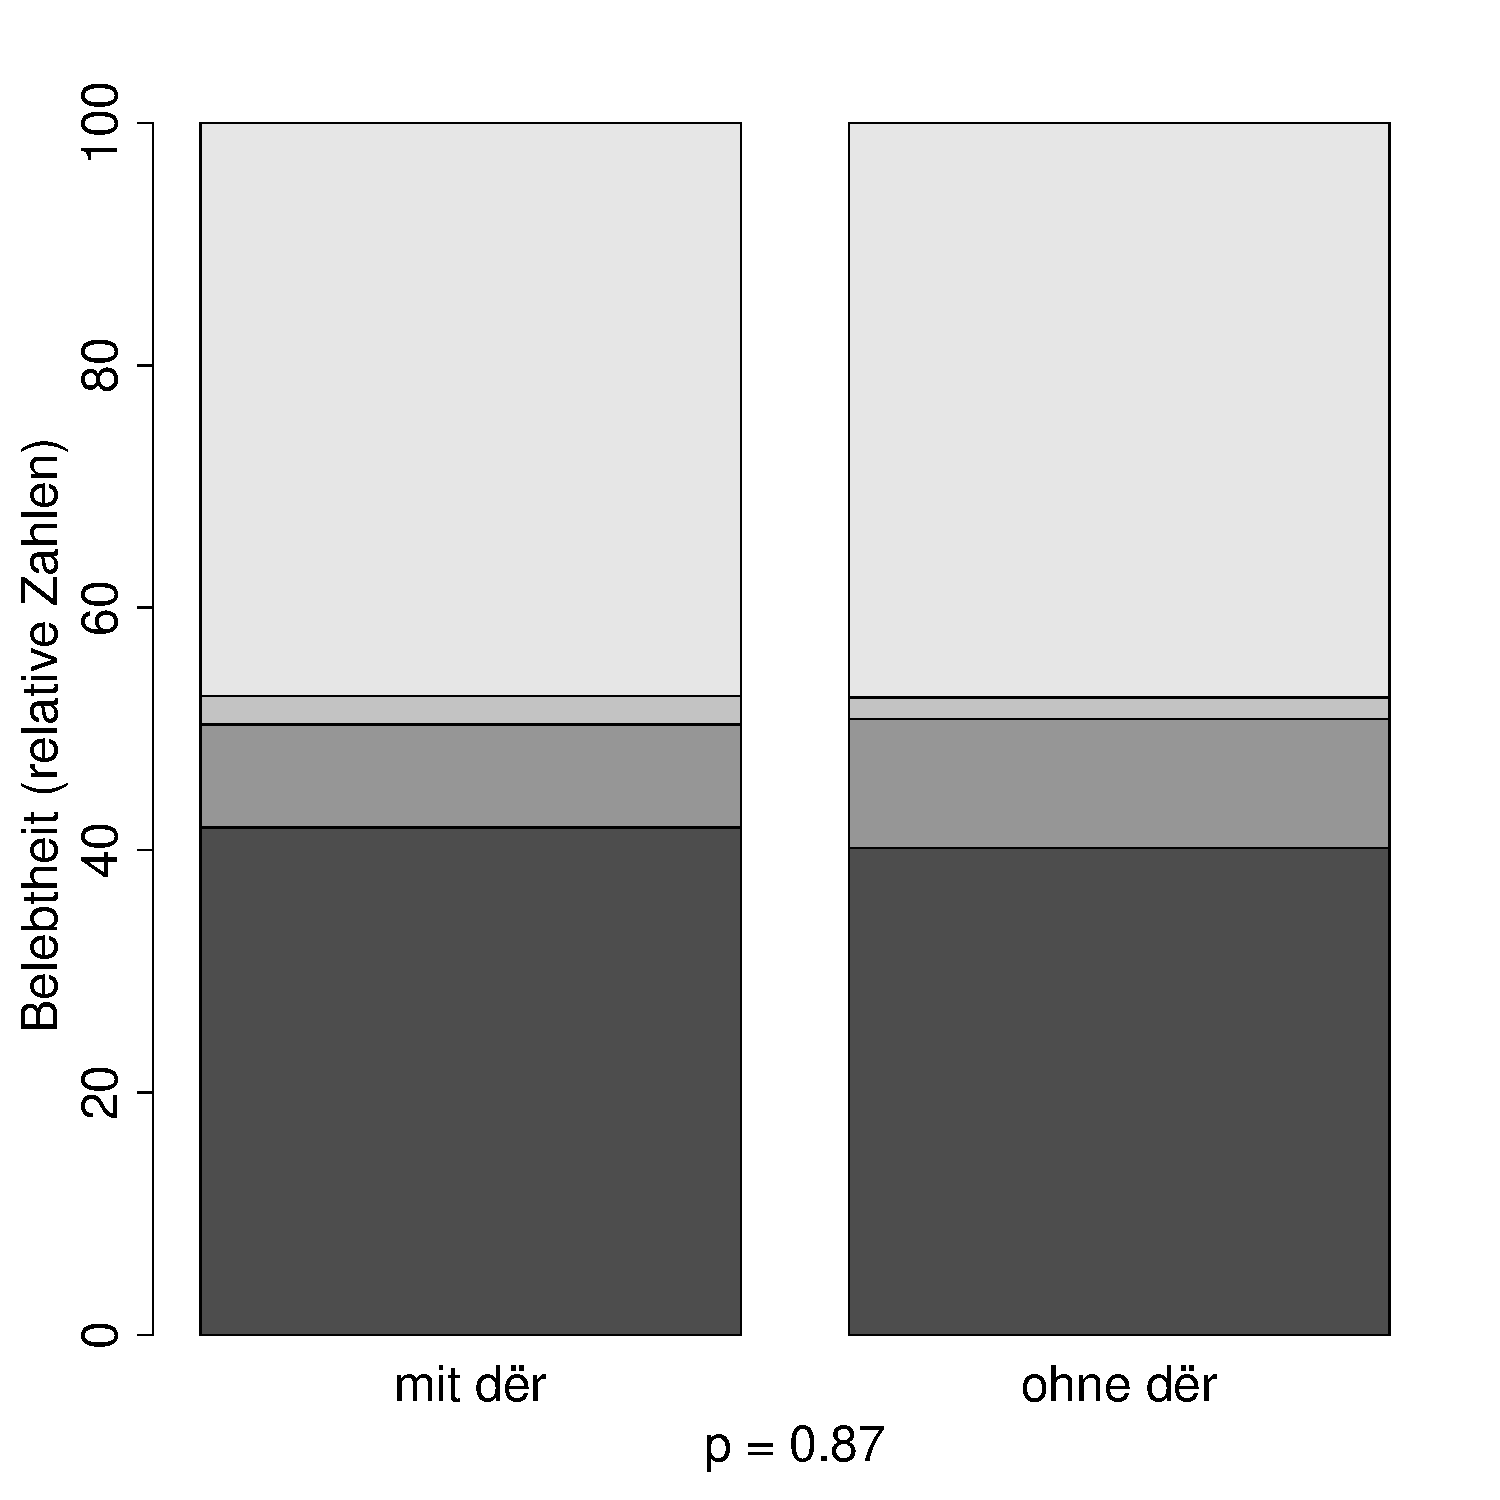
\includegraphics[height=.25\textheight]{generated/images/belebtheit-I}
\caption {Isidor}
\end{subfigure}%
\begin{subfigure}[b]{.5\linewidth}
  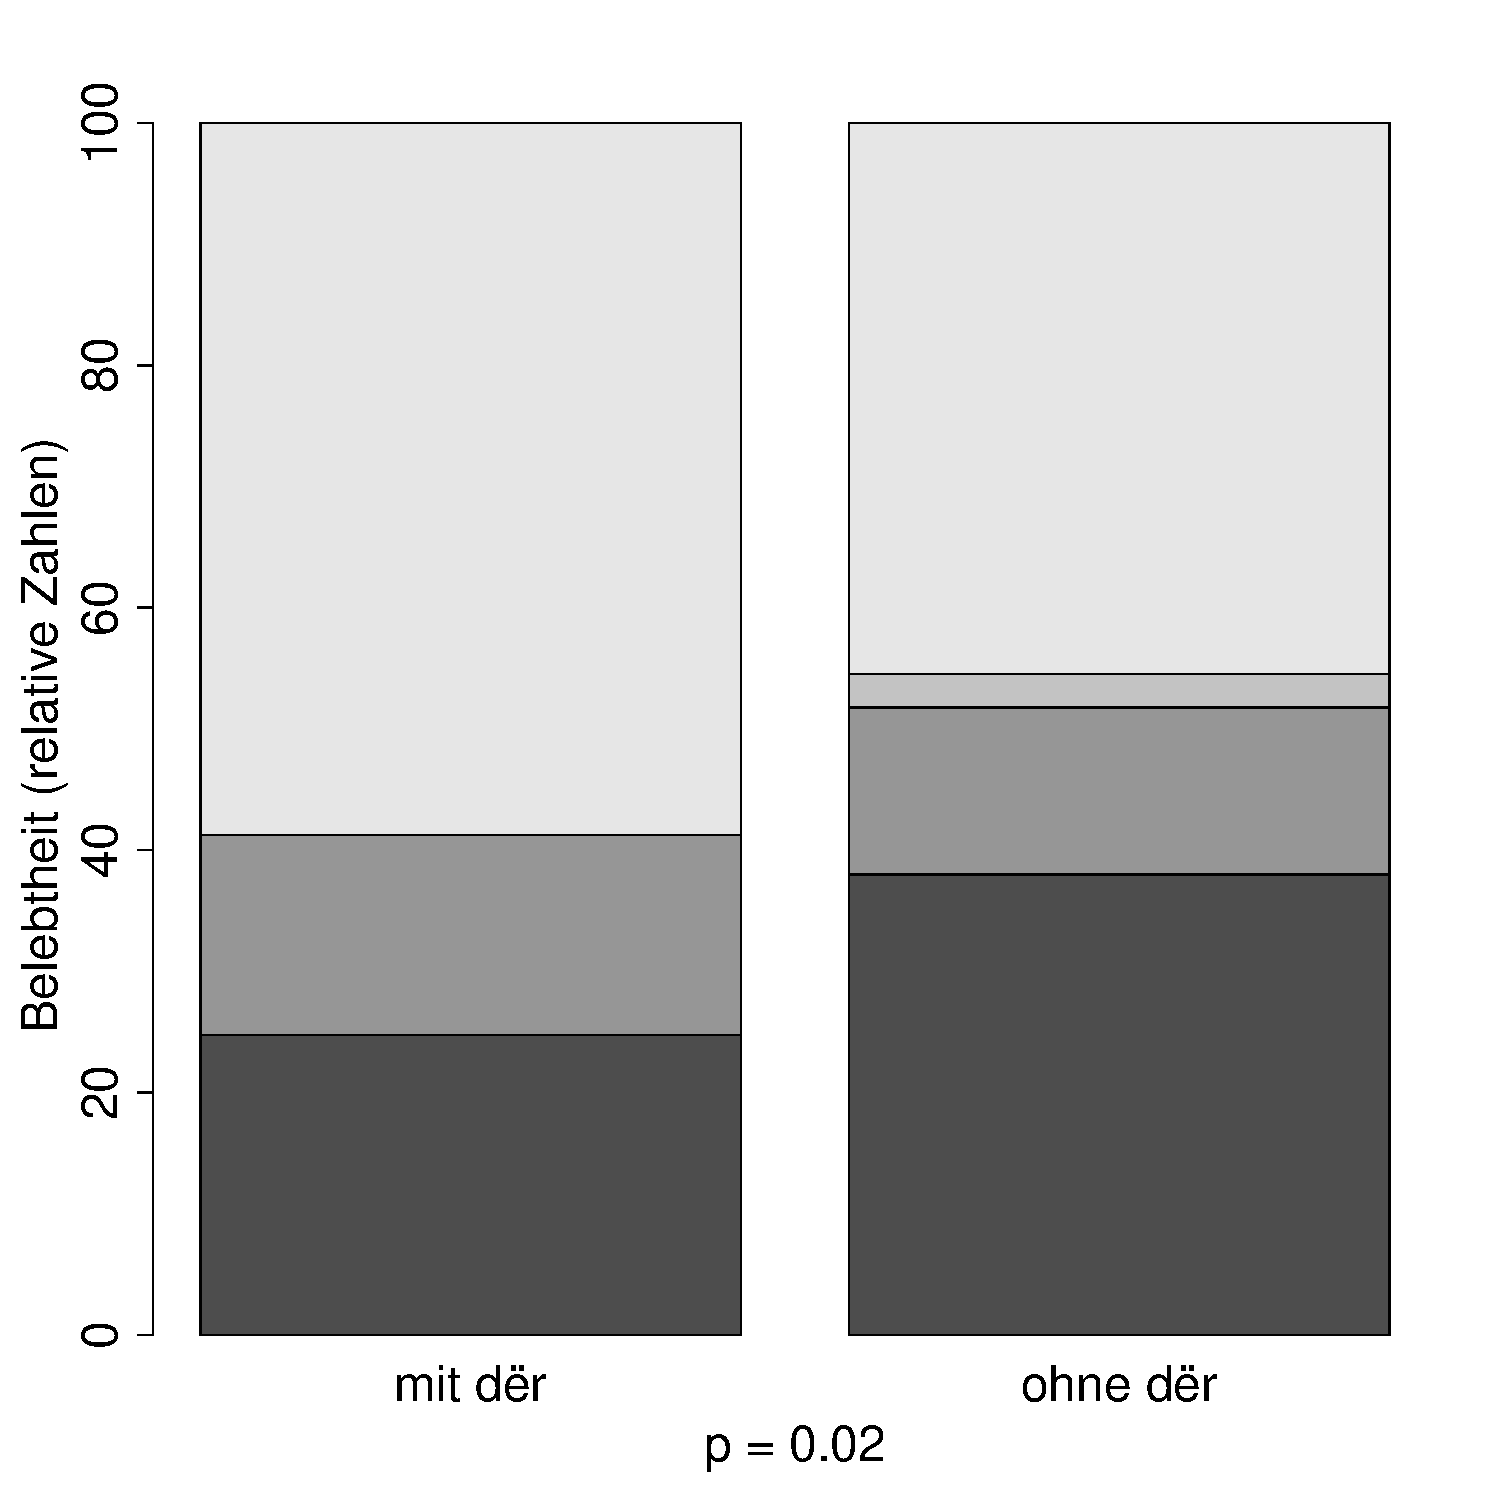
\includegraphics[height=.25\textheight]{generated/images/belebtheit-M}
\caption {Monseer Matthäus}
\end{subfigure}

\begin{subfigure}[b]{.5\linewidth}
  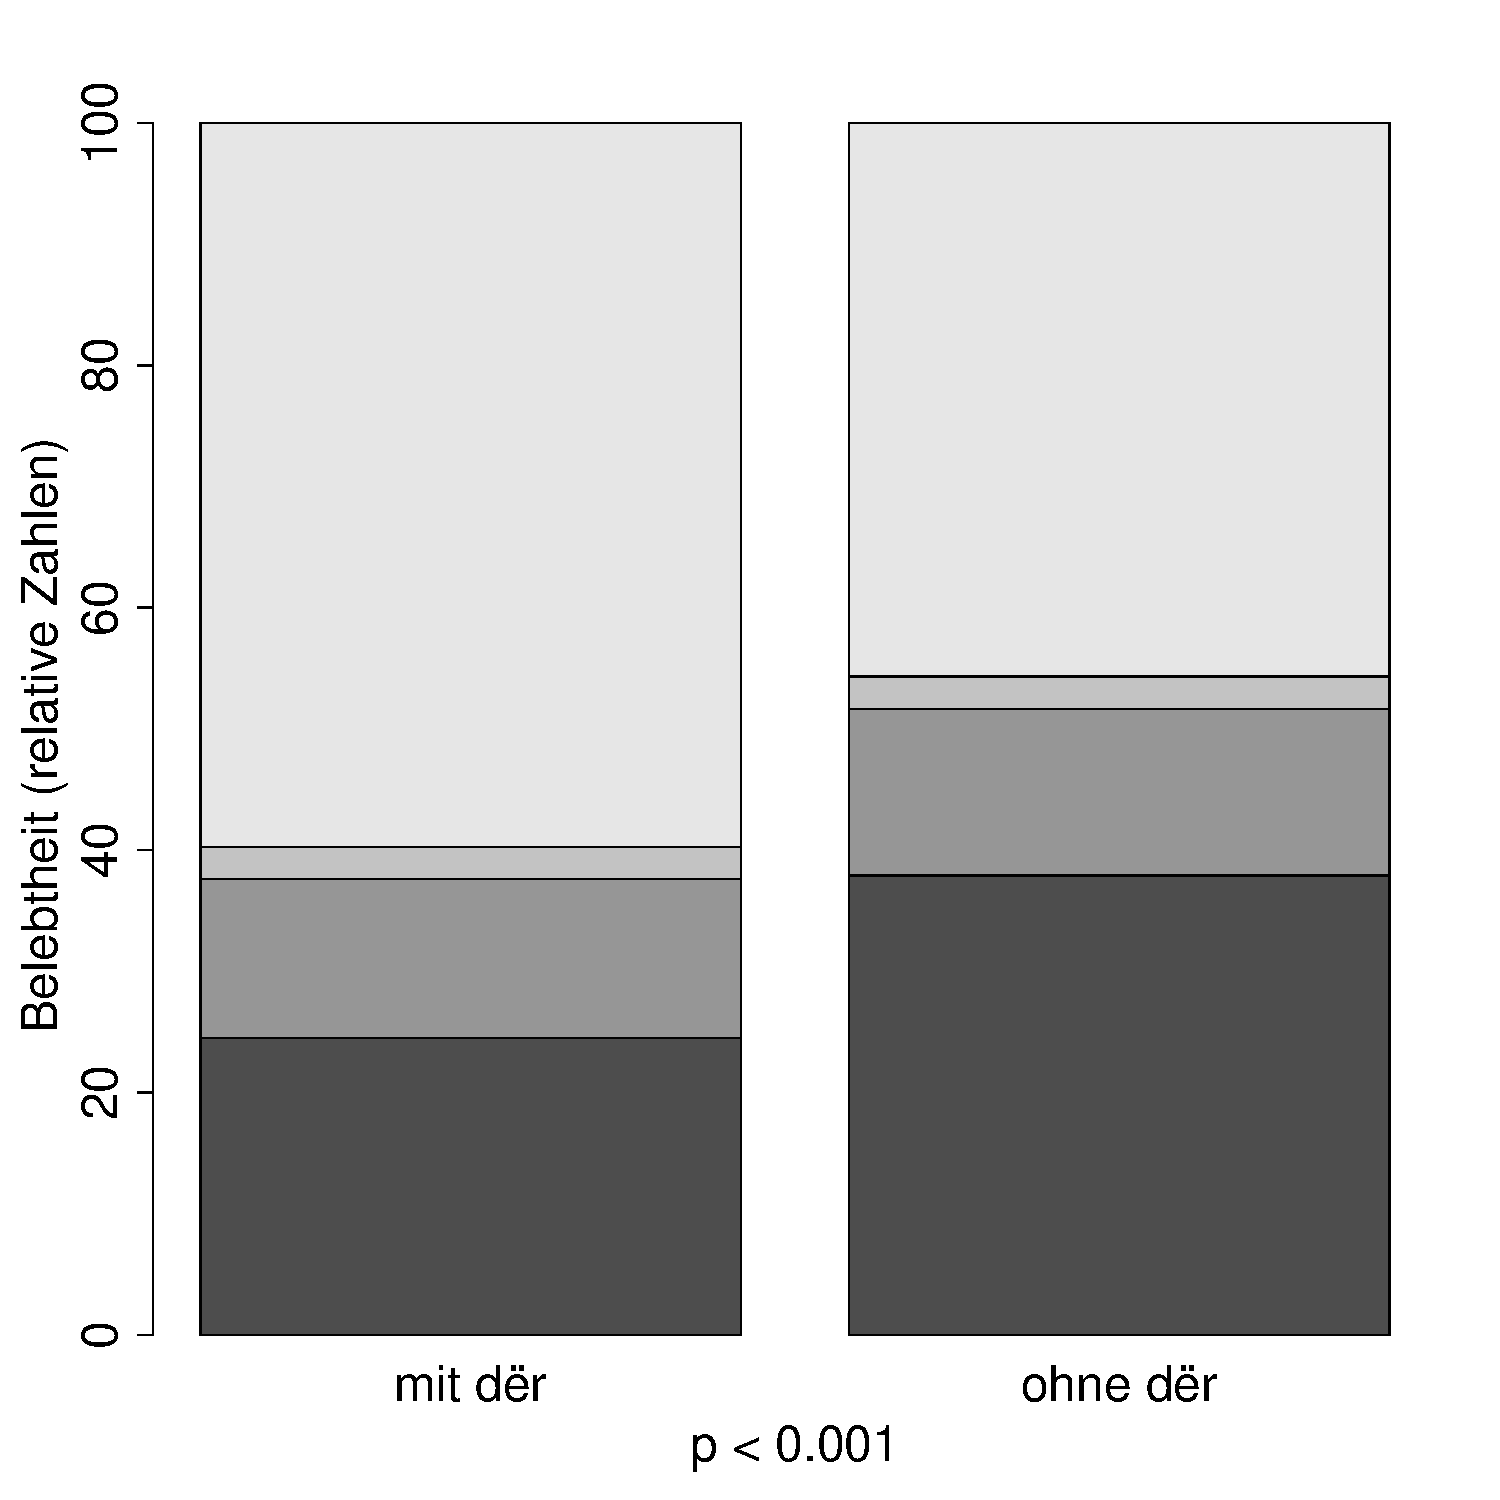
\includegraphics[height=.25\textheight]{generated/images/belebtheit-T}
\caption {Tatian}
\end{subfigure}%
\begin{subfigure}[b]{.5\linewidth}
  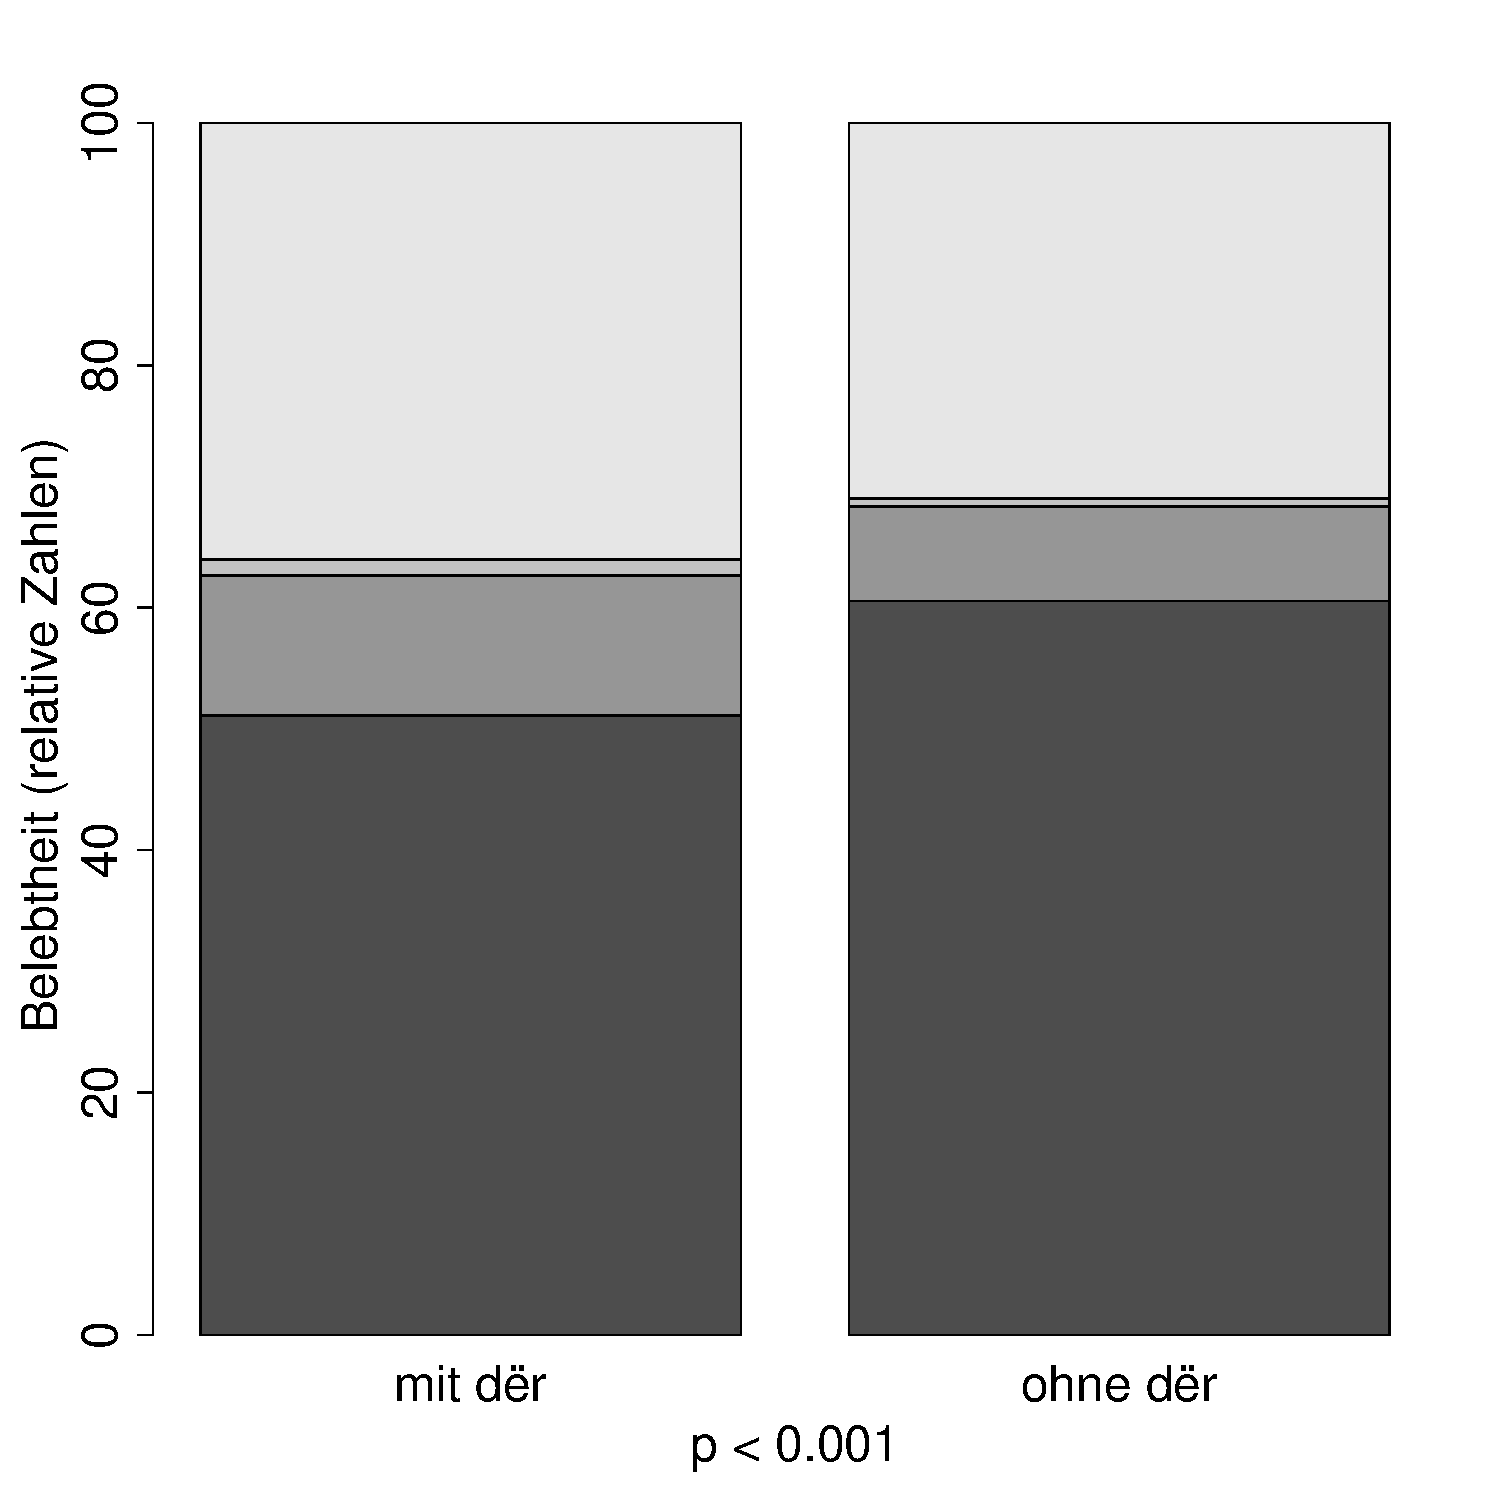
\includegraphics[height=.25\textheight]{generated/images/belebtheit-O}
\caption {Otfrid}
\end{subfigure}

\begin{subfigure}[b]{.5\linewidth}
  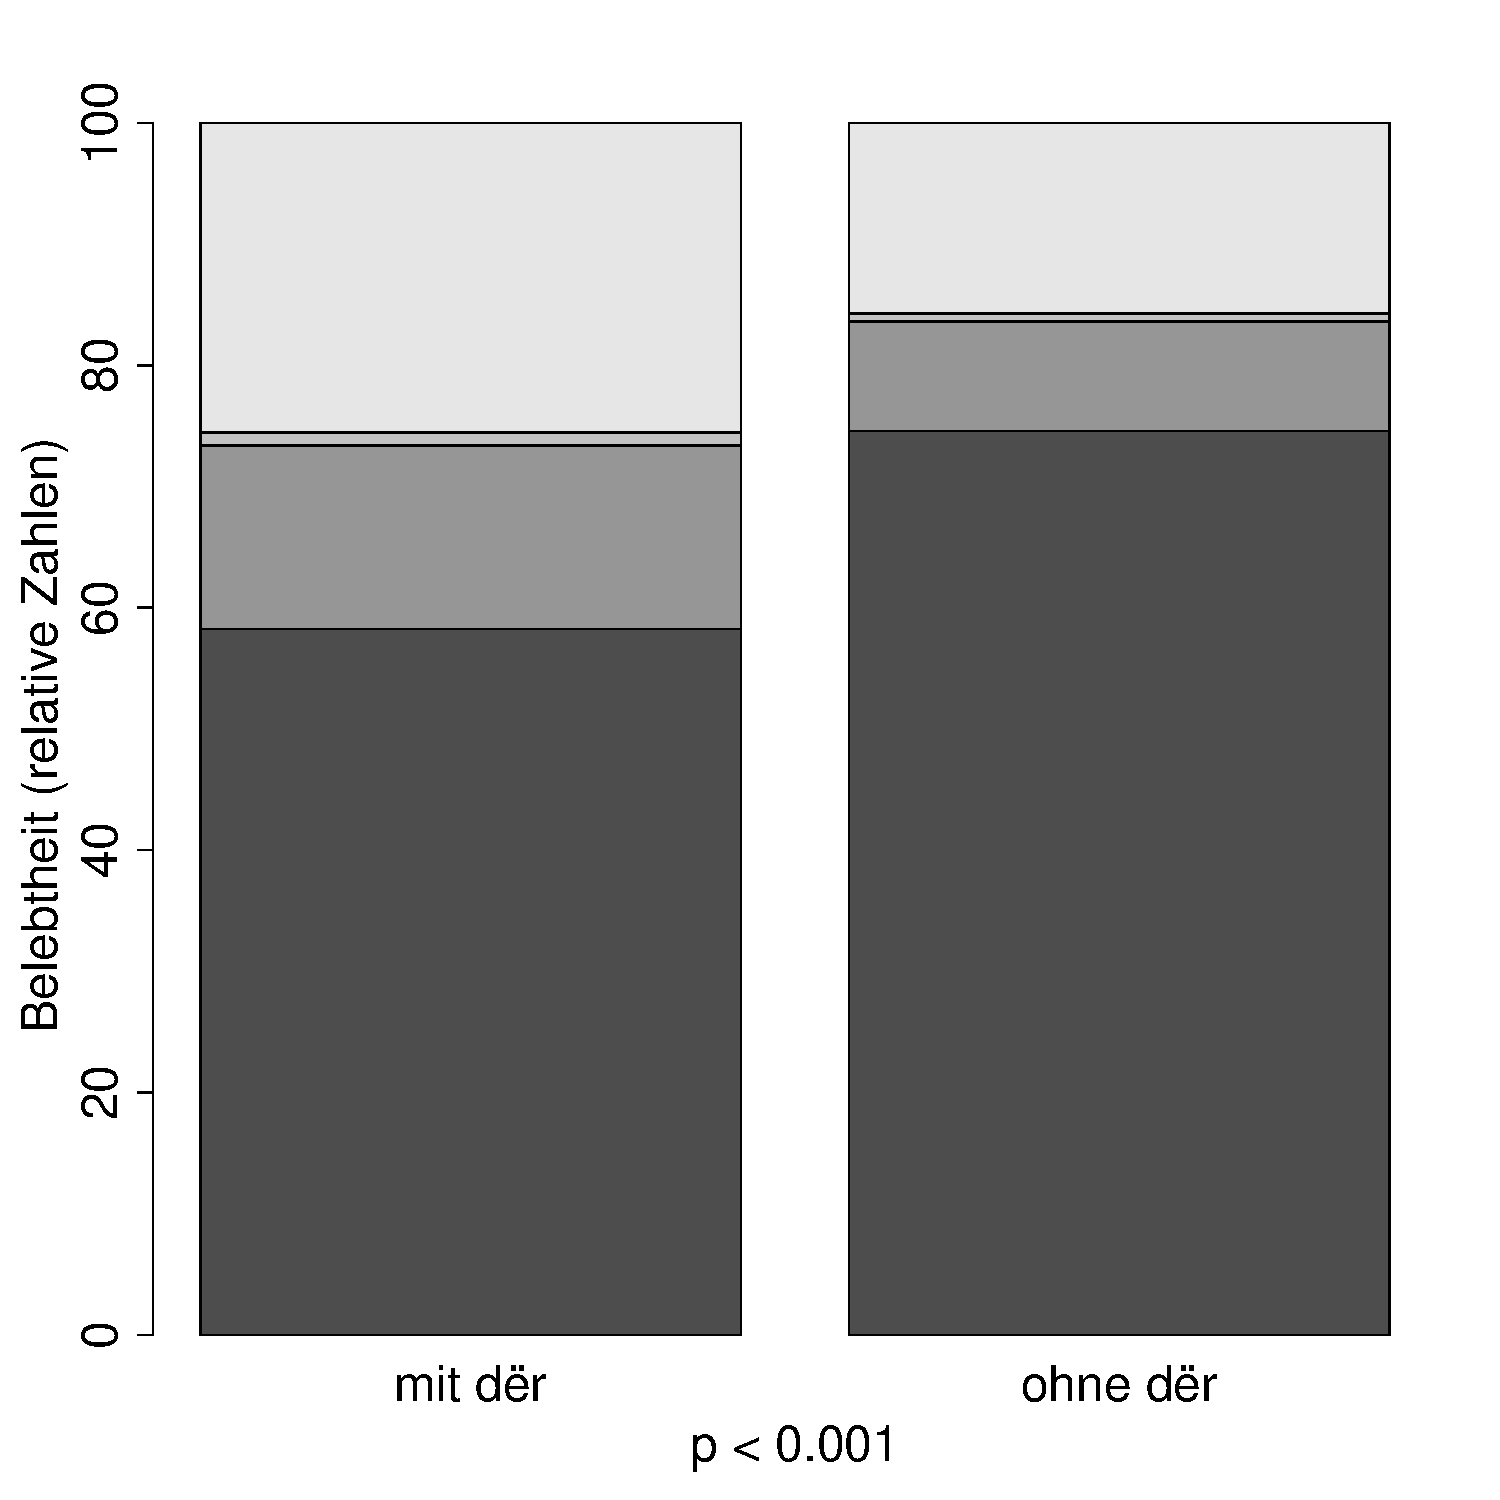
\includegraphics[height=.25\textheight]{generated/images/belebtheit-N}
\caption {Notker}
\end{subfigure}%
\begin{subfigure}[b]{.5\linewidth}
  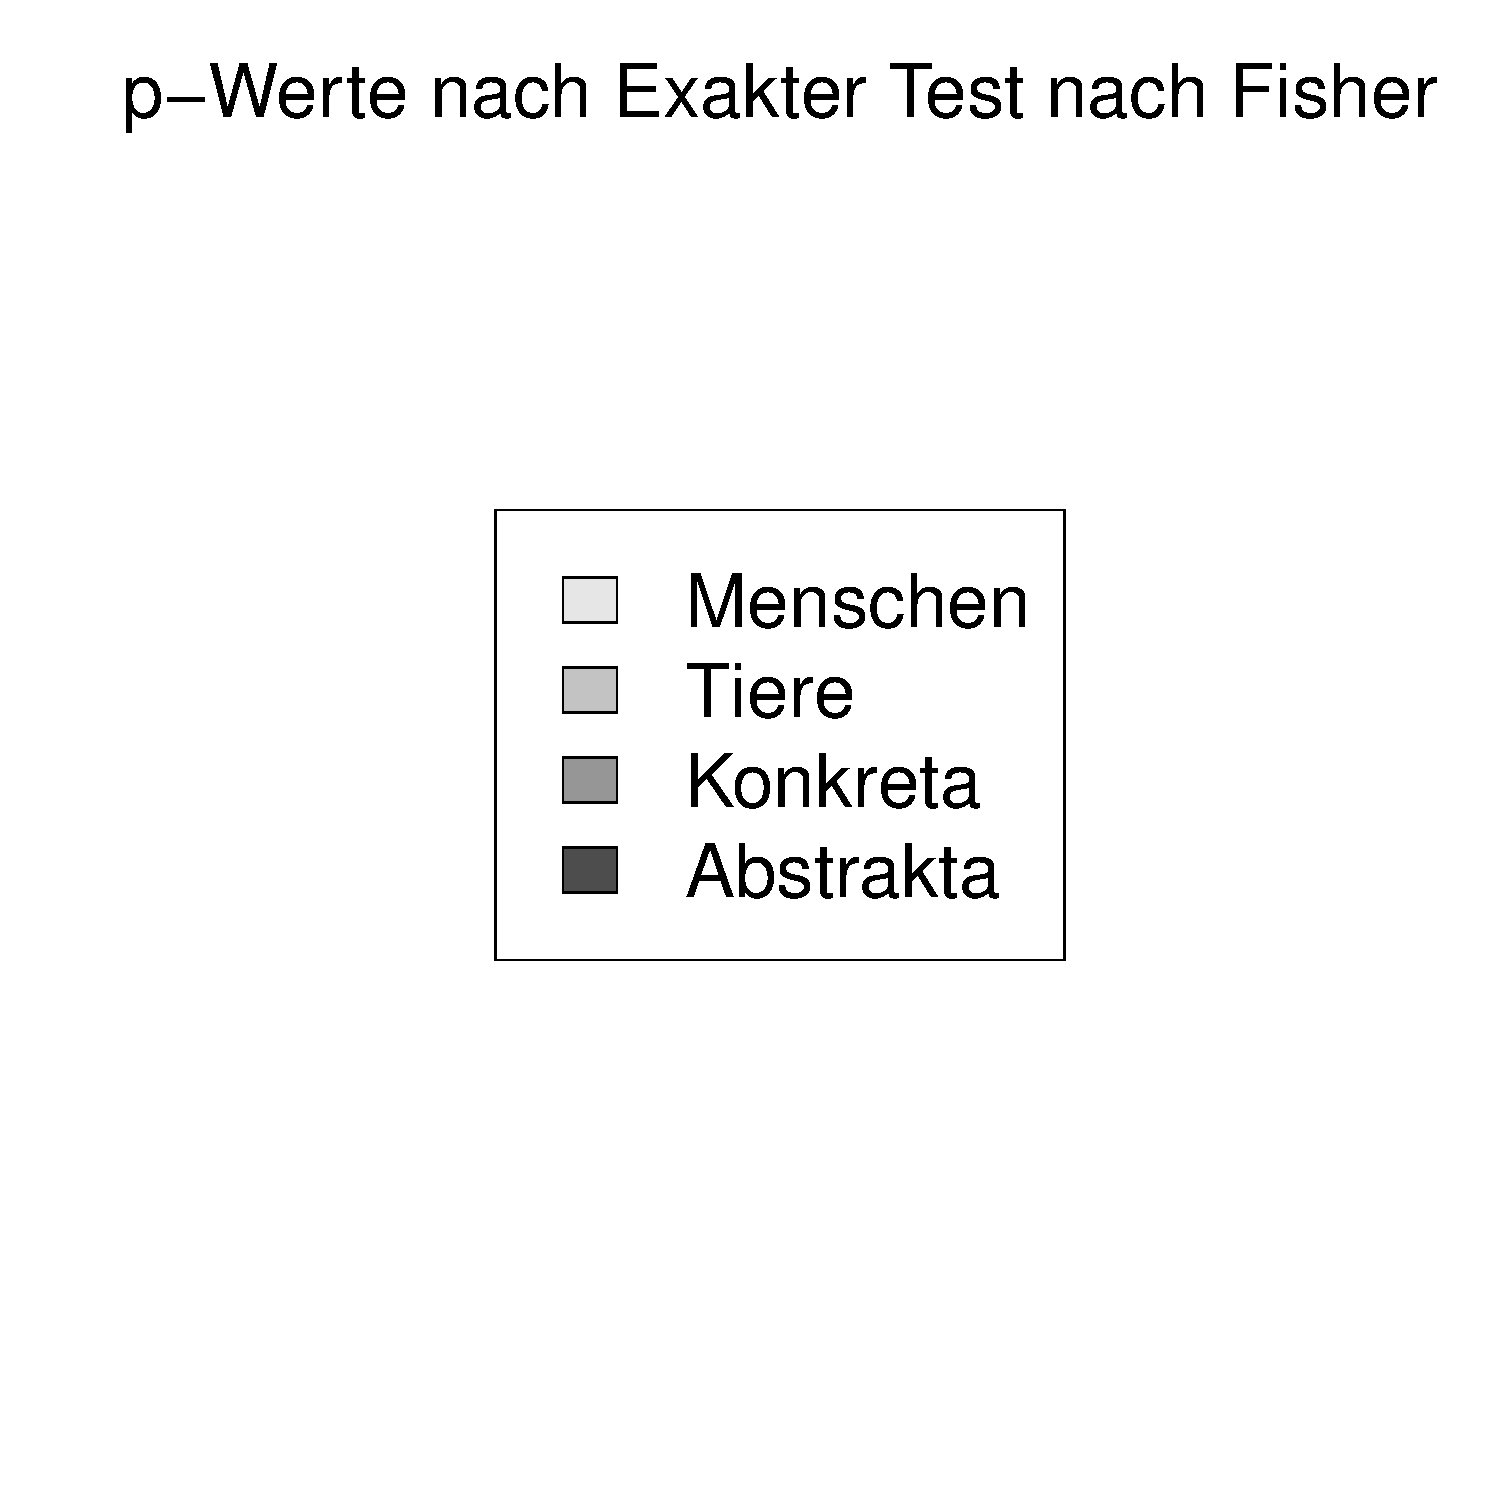
\includegraphics[height=.25\textheight]{generated/images/belebtheit-legende}
\end{subfigure}

\caption{Der Gebrauch von \object{dër} in Korrelation mit den Belebtheitsbasiskategorien}
\label{fig:bel-basis}
\end{figure}

%\inputtable{generated/tables/bel.abs-I}{Gebrauch von \object{dër} in Korrelation mit Belebtheit; \\Isidor, absolute Zahlen}{tab:I}
%\inputtable{generated/tables/bel.abs-M}{Gebrauch von \object{dër} in Korrelation mit Belebtheit; \\Monseer Matthäus, absolute Zahlen}{tab:M}
%\inputtable{generated/tables/bel.abs-T}{Gebrauch von \object{dër} in Korrelation mit Belebtheit; \\Tatian, absolute Zahlen}{tab:T}
%\inputtable{generated/tables/bel.abs-O}{Gebrauch von \object{dër} in Korrelation mit Belebtheit; \\Otfrid, absolute Zahlen}{tab:O}
%\enlargethispage{1ex}
%\inputtable{generated/tables/bel.abs-N}{Gebrauch von \object{dër} in Korrelation mit Belebtheit; \\Notker, absolute Zahlen}{tab:N}

\begin{table}
\begin{tabular}{lrrrrrr}
  \lsptoprule
{Text} & {Struktur} & {Menschen} & {Tiere} & {Konkreta} & {Abstrakta} & {Summe} \\ 
  \midrule
I & mit \object{dër} & 61 & 3 & 11 & 54 & 129 \\ 
 & ohne \object{dër} & 236 & 9 & 53 & 200 & 498 \\ 
 & Summe & 297 & 12 & 64 & 254 & 627 \\ 
   \midrule
M & mit \object{dër} & 57 & 0 & 16 & 24 & 97 \\ 
 & ohne \object{dër} & 195 & 12 & 59 & 163 & 429 \\ 
 & Summe & 252 & 12 & 75 & 187 & 526 \\ 
  \midrule
T & mit \object{dër} & 478 & 21 & 105 & 196 & 800 \\ 
 & ohne \object{dër} & 1333 & 78 & 402 & 1106 & 2919 \\ 
 & Summe & 1811 & 99 & 507 & 1302 & 3719 \\ 
  \midrule
O & mit \object{dër} & 698 & 25 & 224 & 990 & 1937 \\ 
 & ohne \object{dër} & 1490 & 33 & 375 & 2912 & 4810 \\ 
 & Summe & 2188 & 58 & 599 & 3902 & 6747 \\ 
  \midrule
N & mit \object{dër} & 96 & 4 & 57 & 219 & 376 \\ 
 & ohne \object{dër} & 174 & 7 & 100 & 825 & 1106 \\ 
 & Summe & 270 & 11 & 157 & 1044 & 1482 \\ 
   \lspbottomrule
\end{tabular}
\caption{Gebrauch von \object{dër} in Korrelation mit \isi{Belebtheit} (absolute Zahlen)}
\label{tab:bel-abs}
\end{table}

Um zu überprüfen, inwiefern die Häufigkeiten in den einzelnen Kategorien von einer zufälligen Verteilung abweichen, wurden die \hervor{Pearson residuals} \parencite{Gries2012} errechnet. Die Nullhypothese, auf denen die Residuen in Abbildung~\ref{fig:residuals-bel}\footnote{ 
Die Mosaikplots sind folgendermaßen zu lesen: Auf der horizontalen Achse sind die Belege in Appellativa \is{Gattungsname} mit und ohne \object{dër} aufgeteilt. Vertikal sieht man die Anteile der menschlichen, tierischen, konkreten und abstrakten Referenten in diesen Gruppen. Die Einfärbung sowie die Strichart zeigt an, ob eine Belebtheitskategorie \is{Belebtheit} häufiger als erwartet mit bzw. ohne \object{dër} erscheint: Eine blaue Einfärbung mit durchgezogener Umrandung steht für eine Abweichung, die größer ist als erwartet, eine rote Einfärbung mit gestrichelter Linie zeigt an, dass die Abweichung niedriger als erwartet ist -- beides jeweils im Vergleich zu den Nachbarzellen. Je dunkler der Farbton, umso größer ist die Abweichung. Weiße Kästen mit gestrichelten bzw. durchgezogenen Linien spiegeln Tendenzen, aber keine Signifikanz (vgl. auch die Legende an der Seite der Grafiken).} basieren, lautet: Die \isi{Belebtheit} hat keinen Einfluss auf die Setzung von \object{dër}. 

Bei Isidor und dem Monseer Matthäus erlauben es die Daten nicht, die Nullhypothese abzulehnen. Es lässt sich kein Einfluss von der Belebtheitskategorie \is{Belebtheit} auf die Artikelsetzung feststellen. Dennoch sieht man in den Monseer Fragmenten eine leichte Affinität von konkreten und menschlichen Referenten zu \object{dër}. Dass im Isidor die Abstrakta \is{Abstraktum} leichter zur \object{dër}-Setzung tendieren als die \is{Konkretum} Konkreta, liegt vermutlich am Thema: Häufig wird auf abstrakte, biblische Referenten wie \object{drinissa} (\extrans{Dreieinigkeit}) oder  \object{megin} (\extrans{Gewalt, Macht}) verwiesen.
 
Im Tatian ist hingegen deutlich zu sehen, dass menschliche Referenten überzufällig häufiger mit \object{dër} determiniert werden als \is{Abstraktum} Abstrakta. Die Abweichungen sind, wie der Fisher Test (Abbildung \ref{fig:bel-basis}) zeigt, auch signifikant. Bei Otfrid neigen nicht nur Menschen, sondern auch  Tierbezeichnungen und Konkreta \is{Konkretum} stärker zur \object{dër}-Setzung. Ein ähnliches Bild zeigt sich bei Notker. Hier ist der Einfluss von \isi{Belebtheit} nicht mehr so stark, aber immer noch signifikant.    

Damit ausgeschlossen werden kann, dass frequente Lemmata \is{Lemma} den Anteil einer Kategorie nach oben treiben und damit das Bild verzerren, wurden die Hapax Legomena separat ausgewertet, s. Abbildung~\ref{fig:residuals-bel-hapaxe}. Bemerkenswert ist, dass nun auch dem Isidor ein höherer Anteil belebter Referenten bei den \object{dër}-Belegen attestiert werden kann. Bei den anderen Denkmälern hat sich mit Ausnahme von Notker das Bild wenig geändert. 

Auch für diese Verteilung wurden Residuen errechnet, s. Abbildung~\ref{fig:bel-hapaxe-residuals}. Es fällt auf, dass bei Otfrid die belebten Referenten signifikant häufiger in der \object{dër}-Gruppe erscheinen als in der Gruppe ohne \object{dër} ($p = 0{,}01$). In den anderen Texten spiegeln die Residuen zwar eine Tendenz, dass belebte und konkrete Referenten häufiger mit \object{dër}-auftreten; die Verteilung ist aber nicht signifikant (vgl. die $p$-Werte in Abbildung~\ref{fig:bel-hapaxe}). Einzig bei Notker, dem jüngsten Text, zeigt sich kein positiver \is{Belebtheit} Belebtheitseffekt. Die Tendenz geht sogar in die andere Richtung: Belebte Hapaxe werden eher nicht mit \object{dër} determiniert. Diese Verteilung ist allerdings nicht signifikant ($p = 0{,}68$).  

\begin{figure}
\begin{subfigure}[b]{.5\linewidth}
  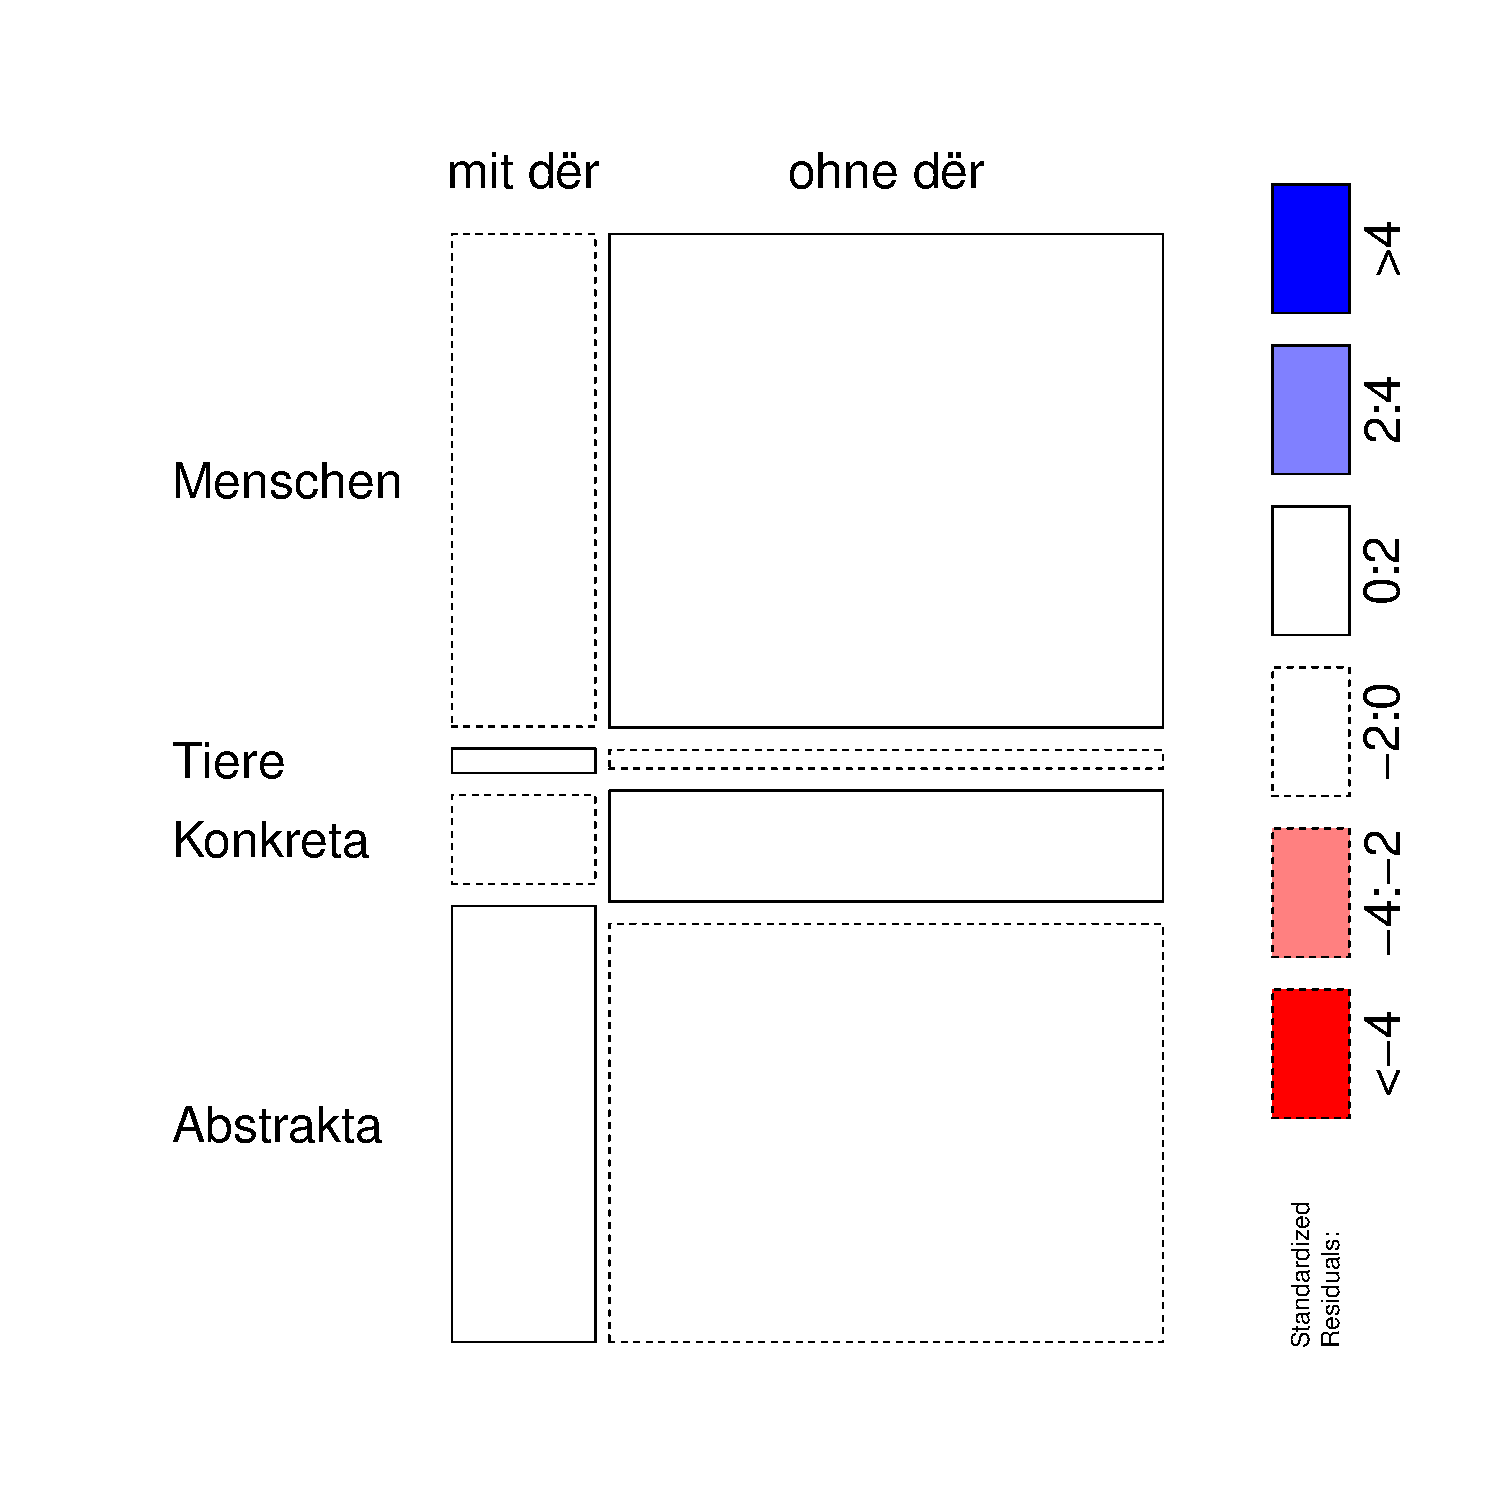
\includegraphics[height=.25\textheight]{generated/images/residuals-bel-I}
\caption {Isidor}
\end{subfigure}%
\begin{subfigure}[b]{.5\linewidth}
  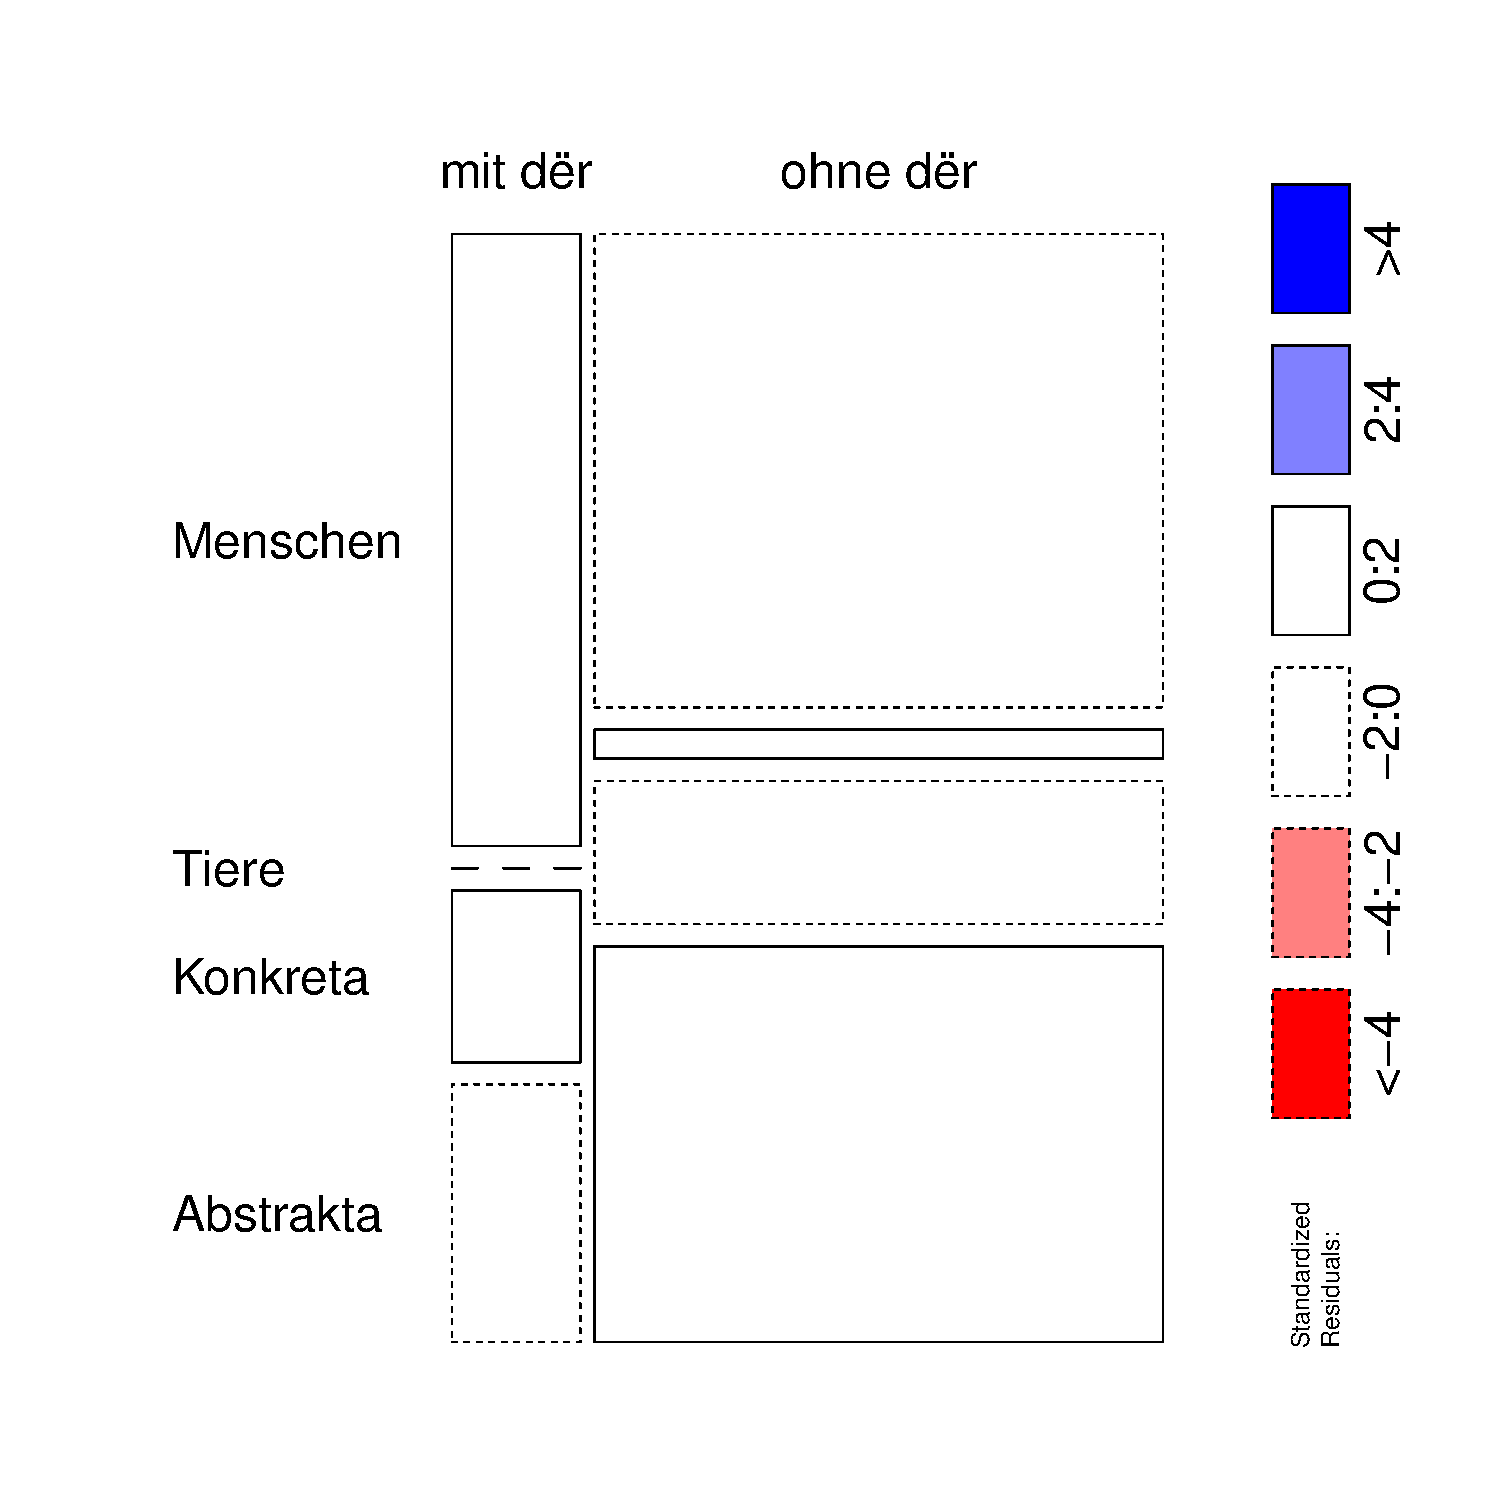
\includegraphics[height=.25\textheight]{generated/images/residuals-bel-M}
\caption {Monseer Matthäus}
\end{subfigure}

\begin{subfigure}[b]{.5\linewidth}
  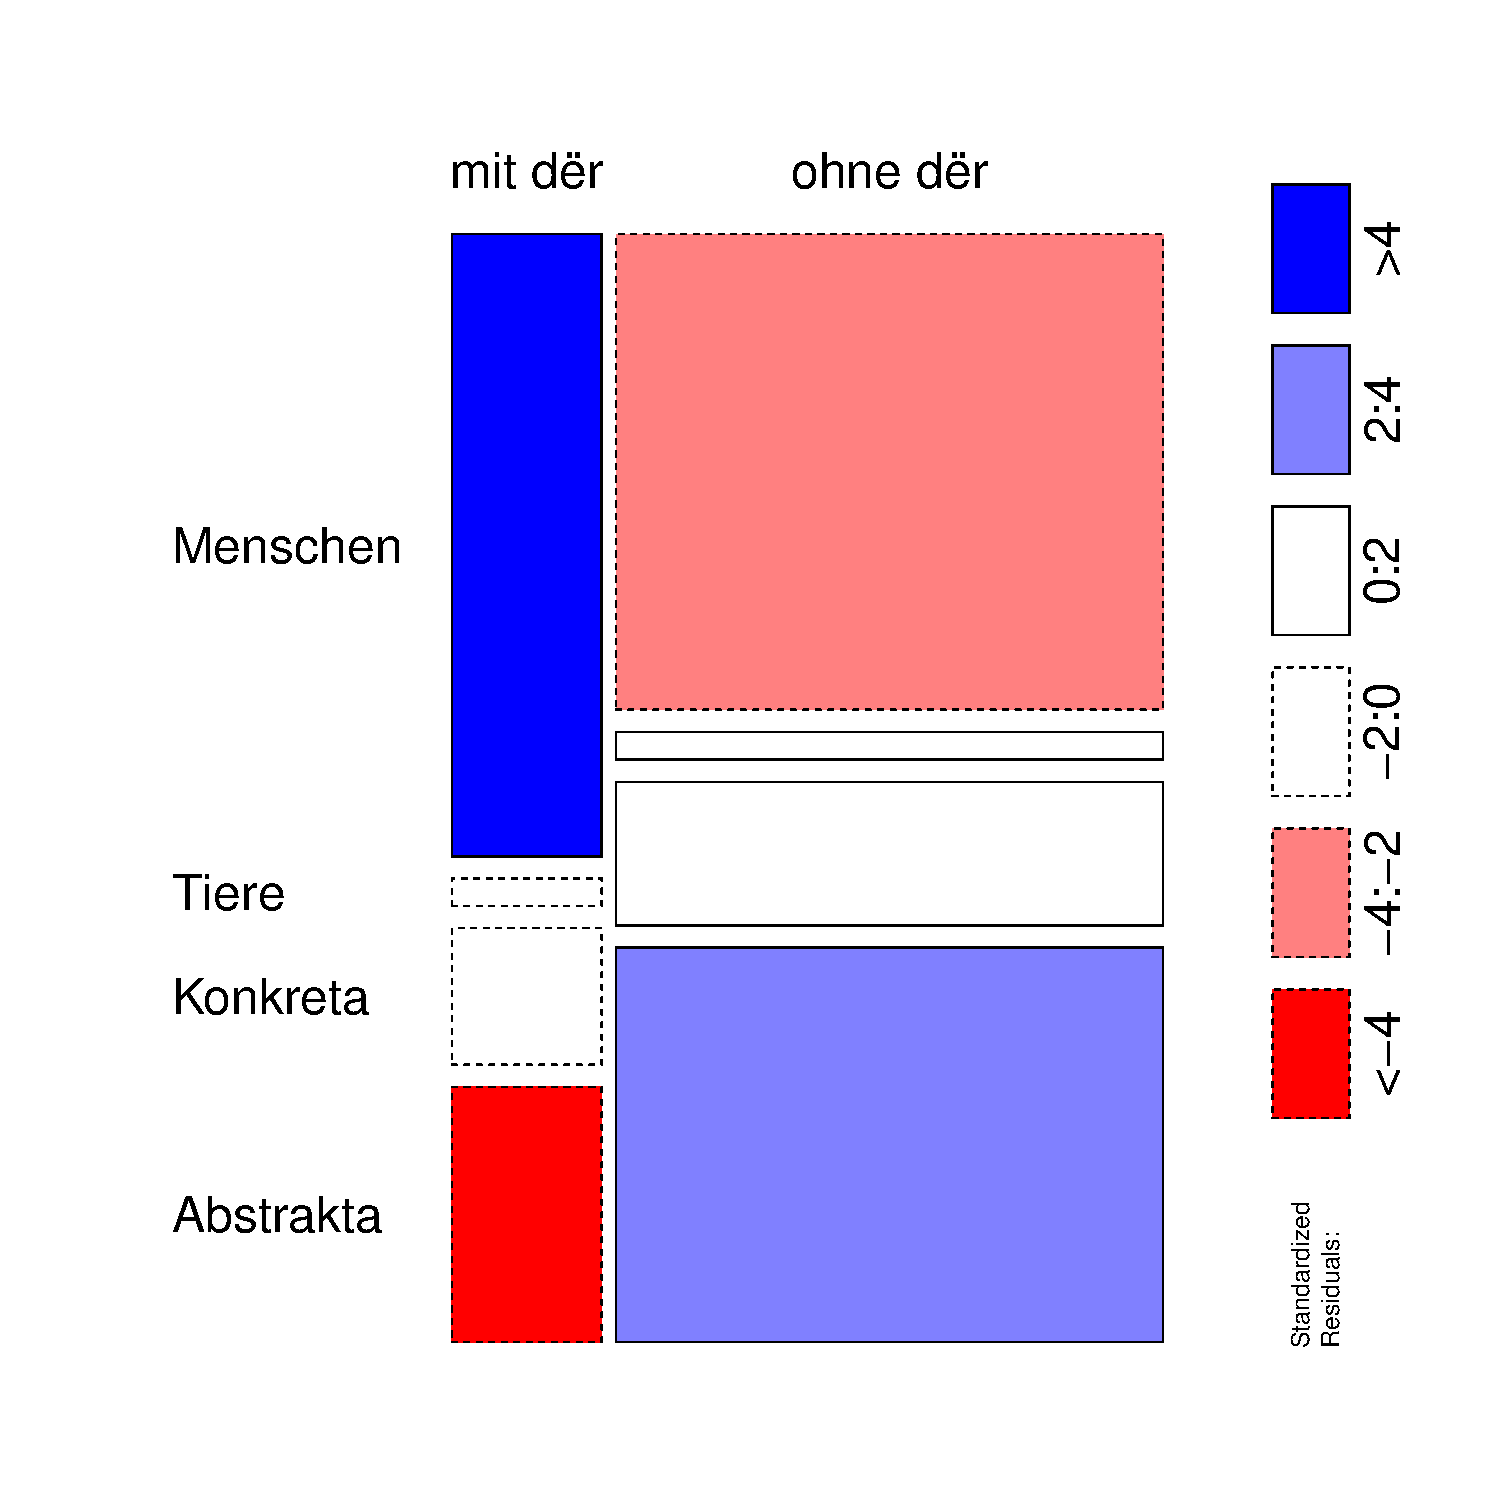
\includegraphics[height=.25\textheight]{generated/images/residuals-bel-T}
\caption {Tatian}
\end{subfigure}%
\begin{subfigure}[b]{.5\linewidth}
  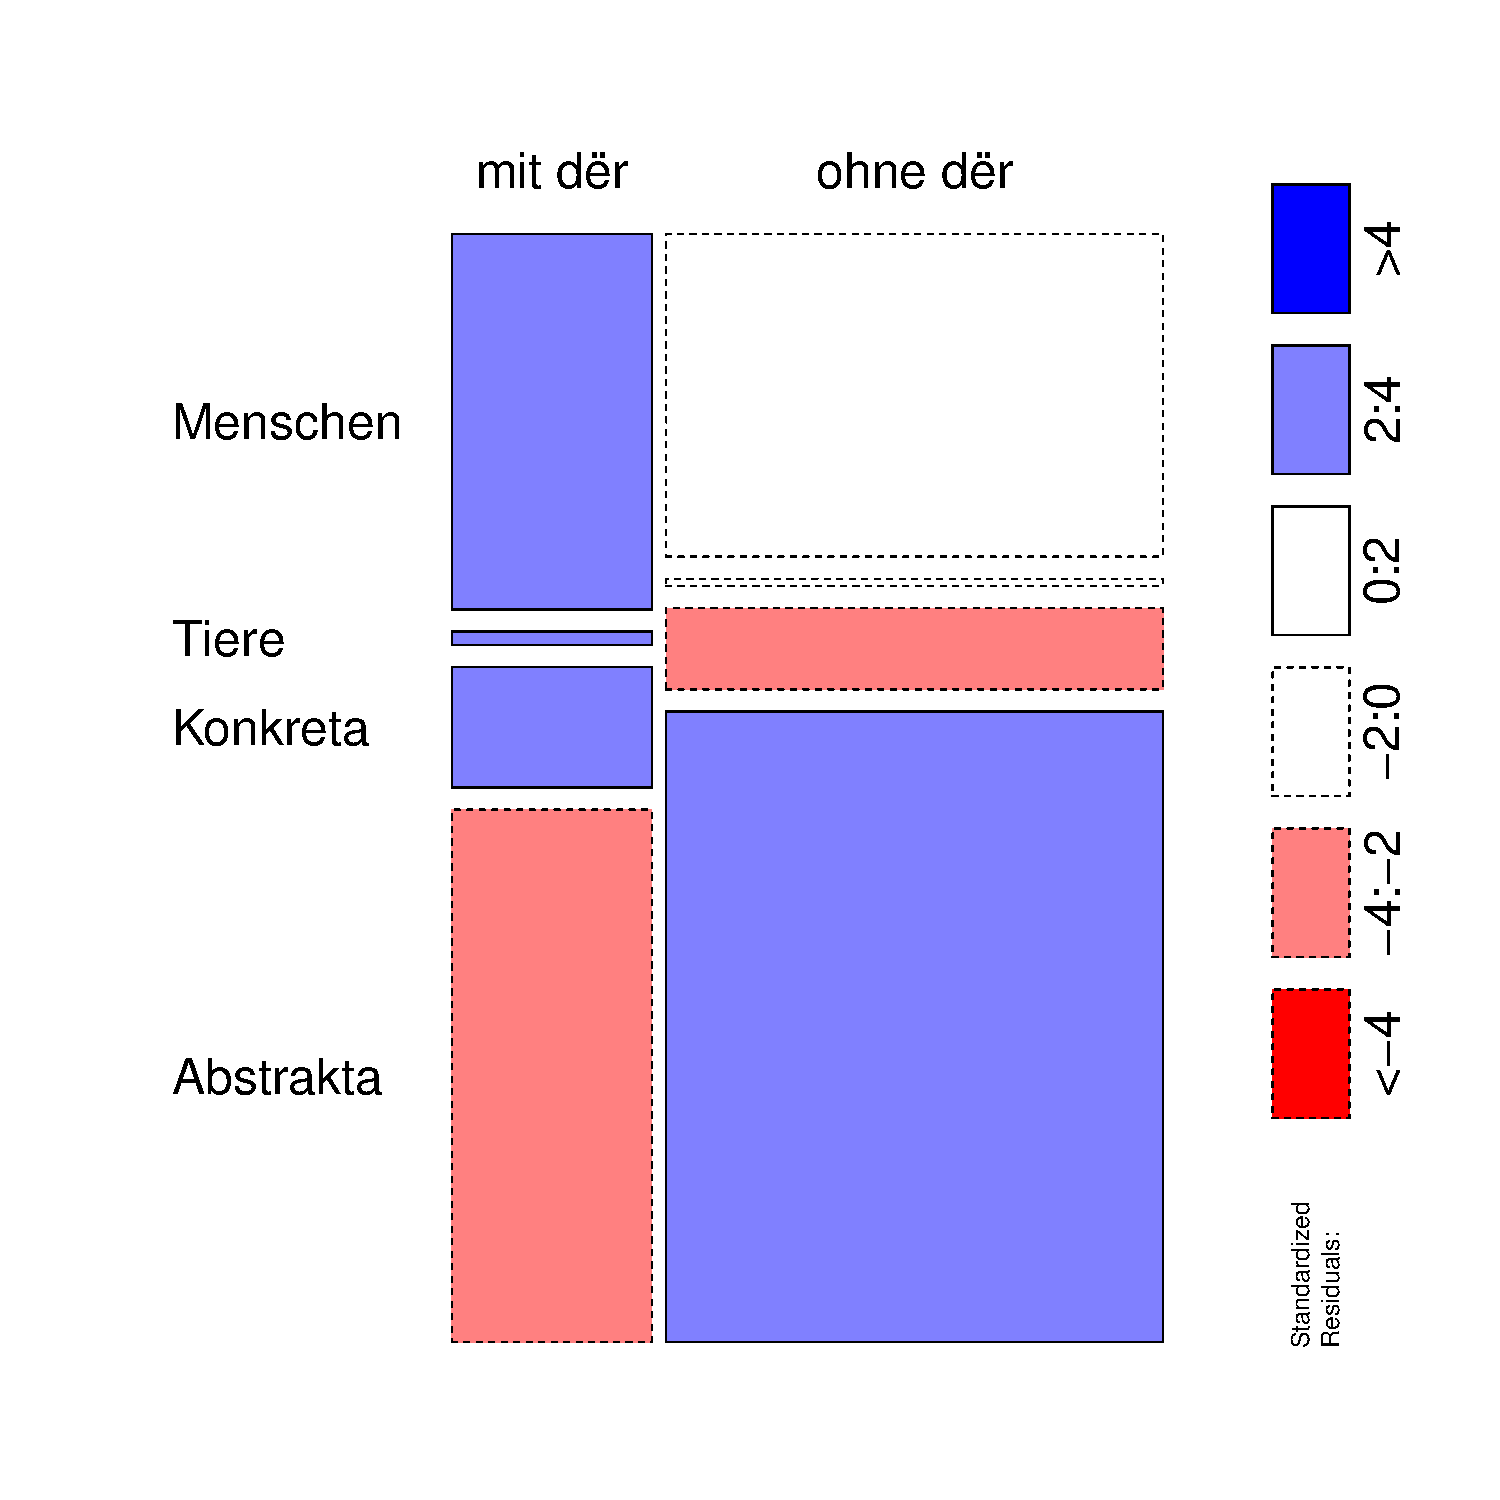
\includegraphics[height=.25\textheight]{generated/images/residuals-bel-O}
\caption {Otfrid}
\end{subfigure}

\begin{subfigure}[b]{.5\linewidth}
  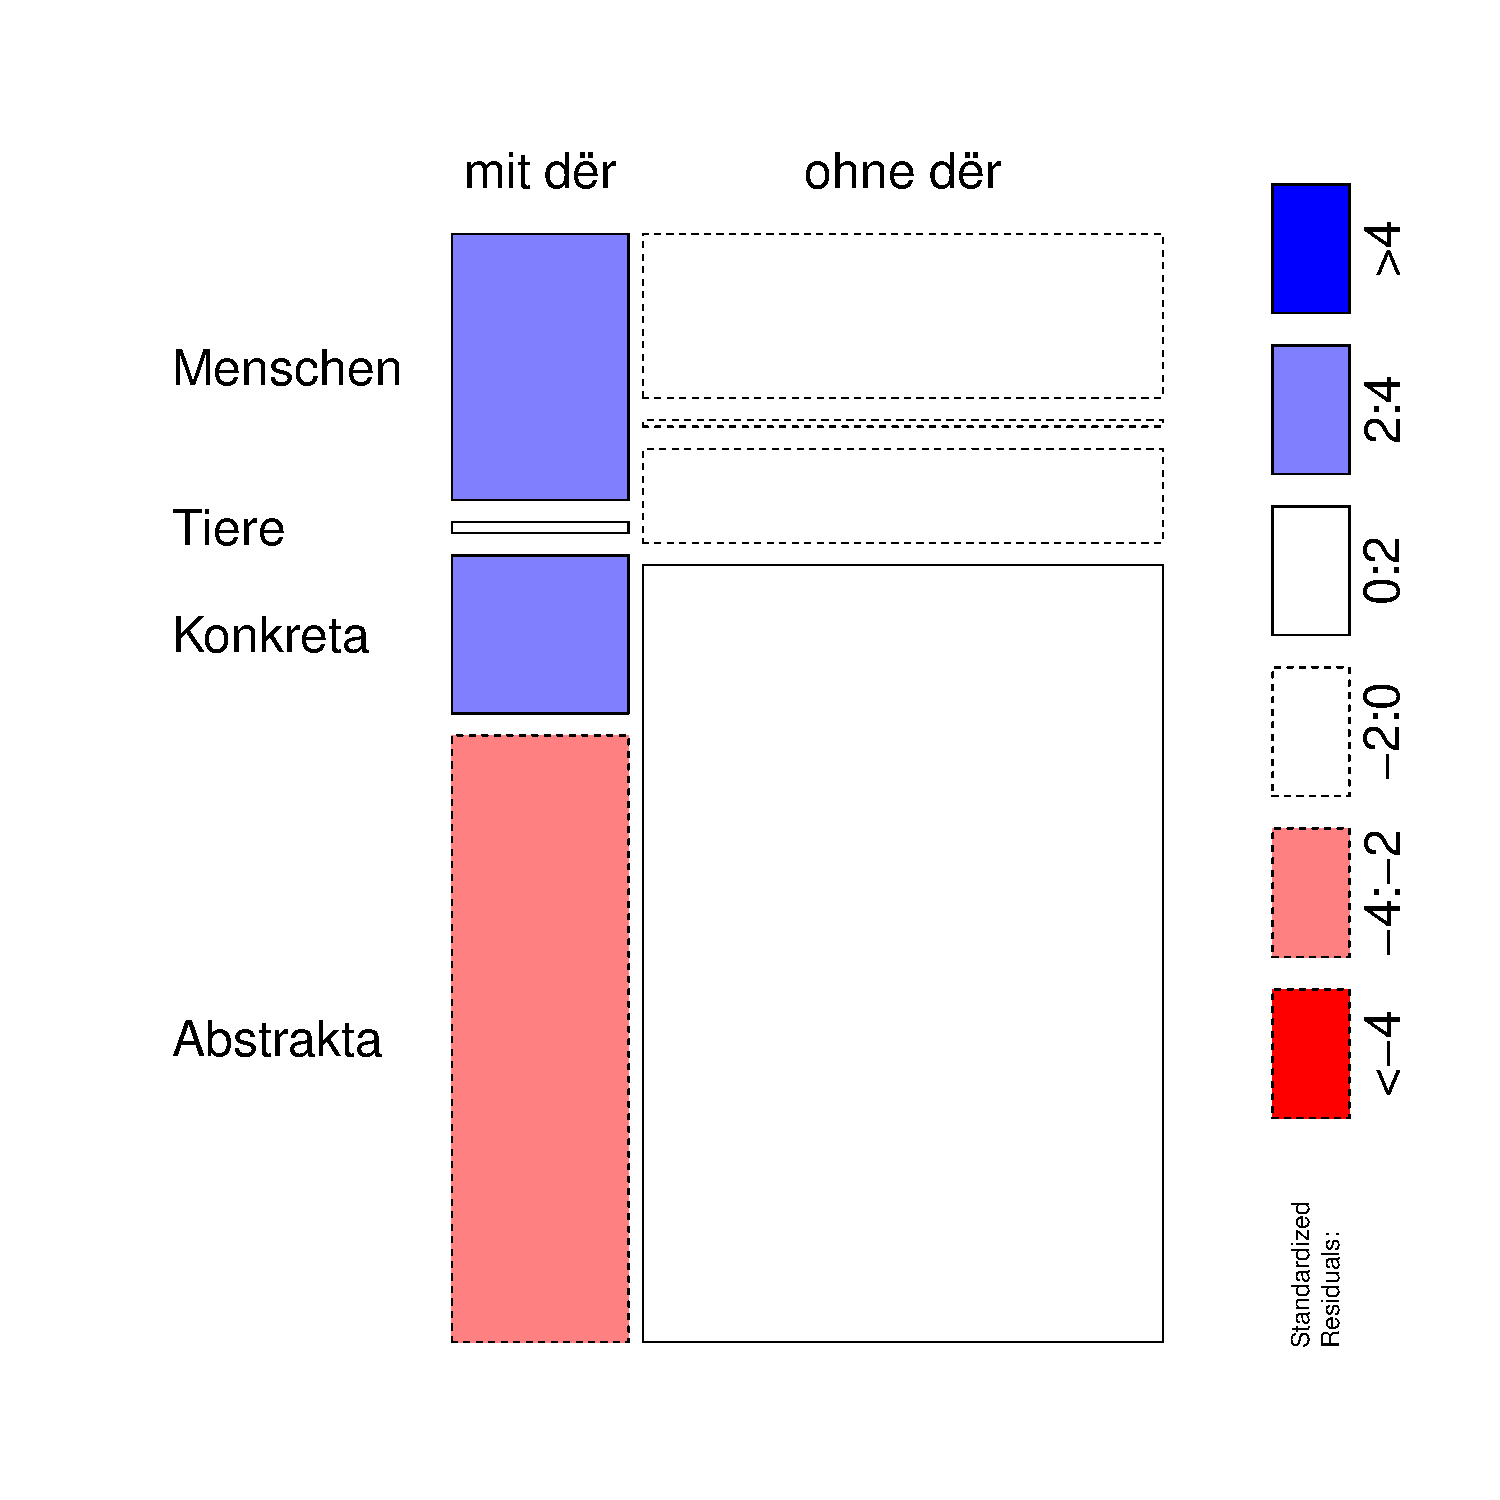
\includegraphics[height=.25\textheight]{generated/images/residuals-bel-N}
\caption {Notker}
\end{subfigure}
\caption{Einfluss von Belebtheit auf \object{dër}-Gebrauch (Residuen)}
\label{fig:residuals-bel}
\end{figure}


\begin{figure}
\begin{subfigure}[b]{.5\linewidth}
  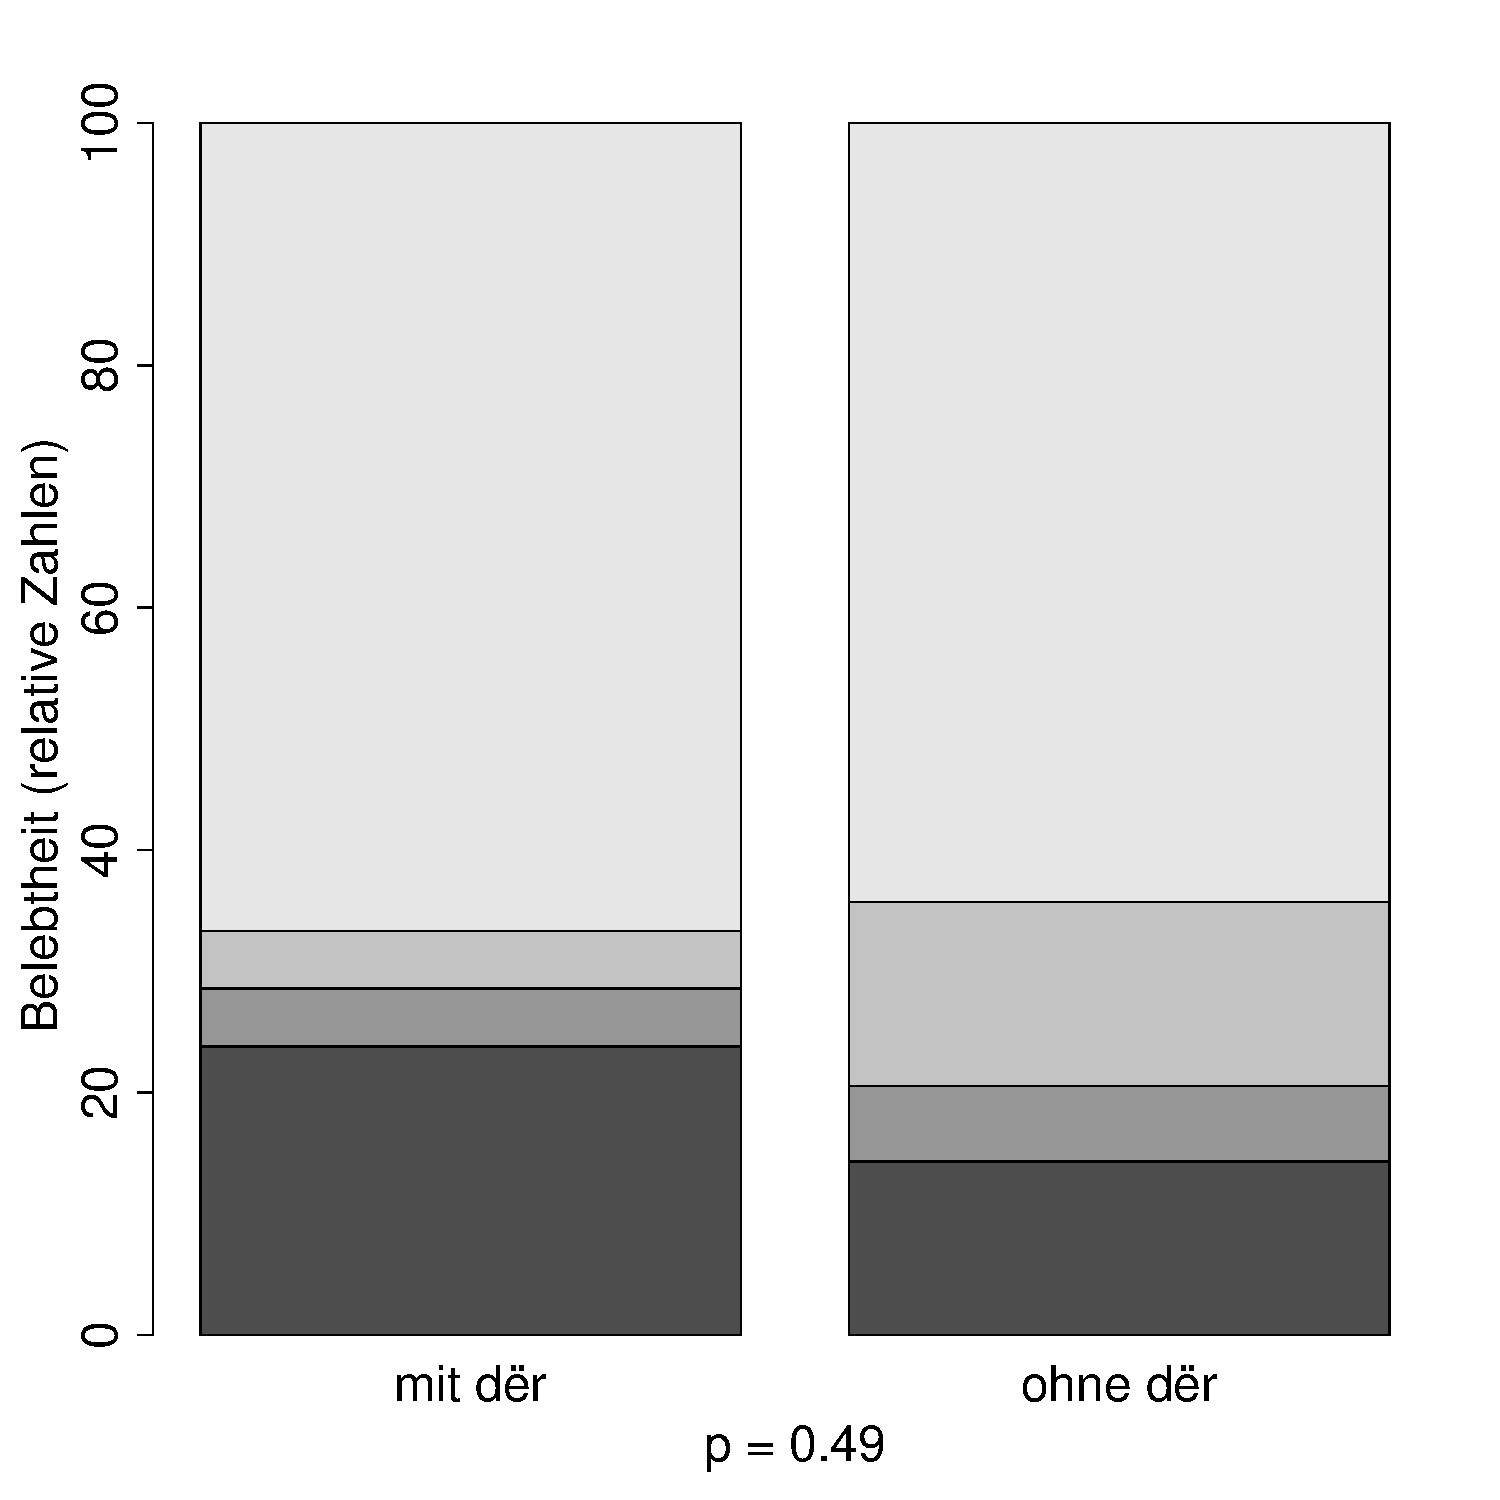
\includegraphics[height=.25\textheight]{generated/images/belebtheit-hapaxe-I}
\caption {Isidor}
\end{subfigure}%
\begin{subfigure}[b]{.5\linewidth}
  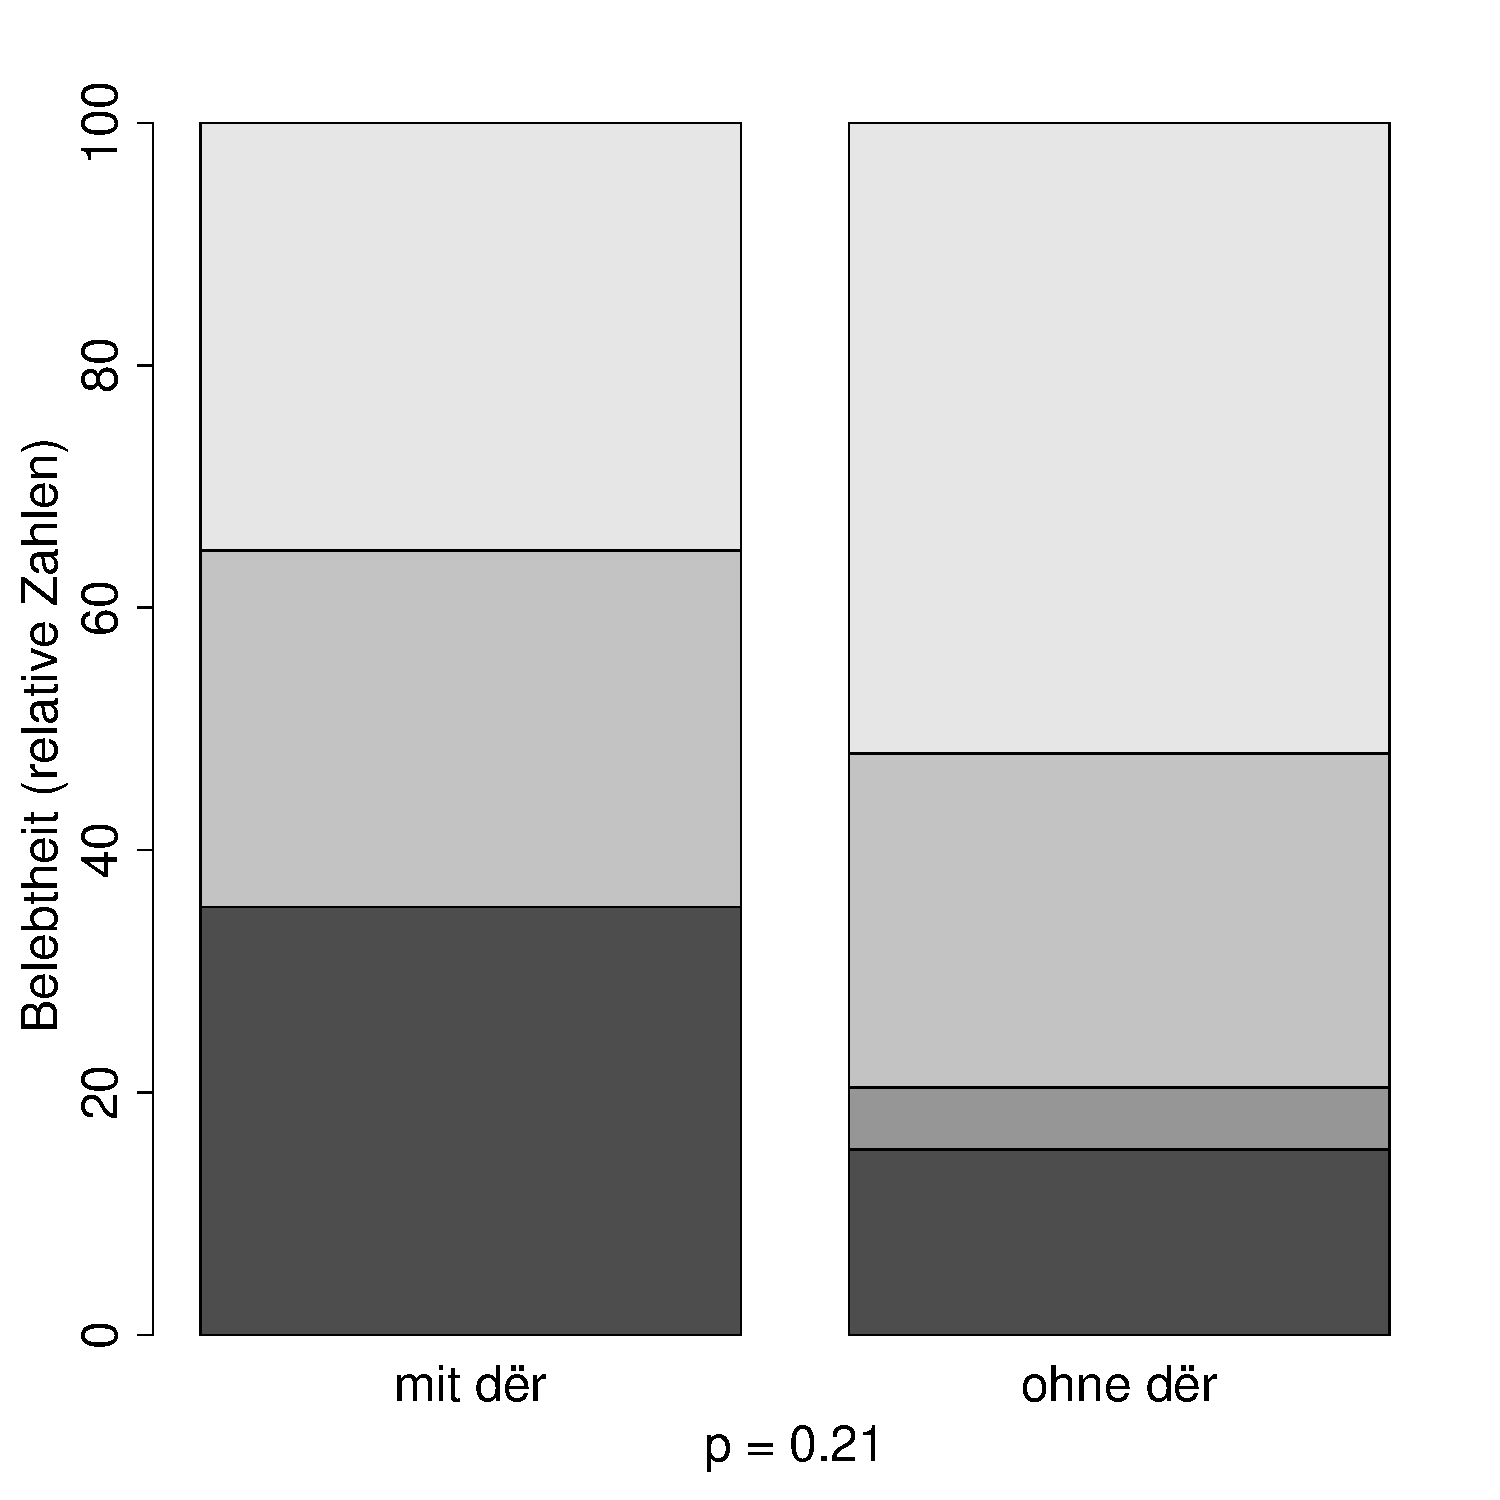
\includegraphics[height=.25\textheight]{generated/images/belebtheit-hapaxe-M}
\caption {Monseer Matthäus}
\end{subfigure}

\begin{subfigure}[b]{.5\linewidth}
  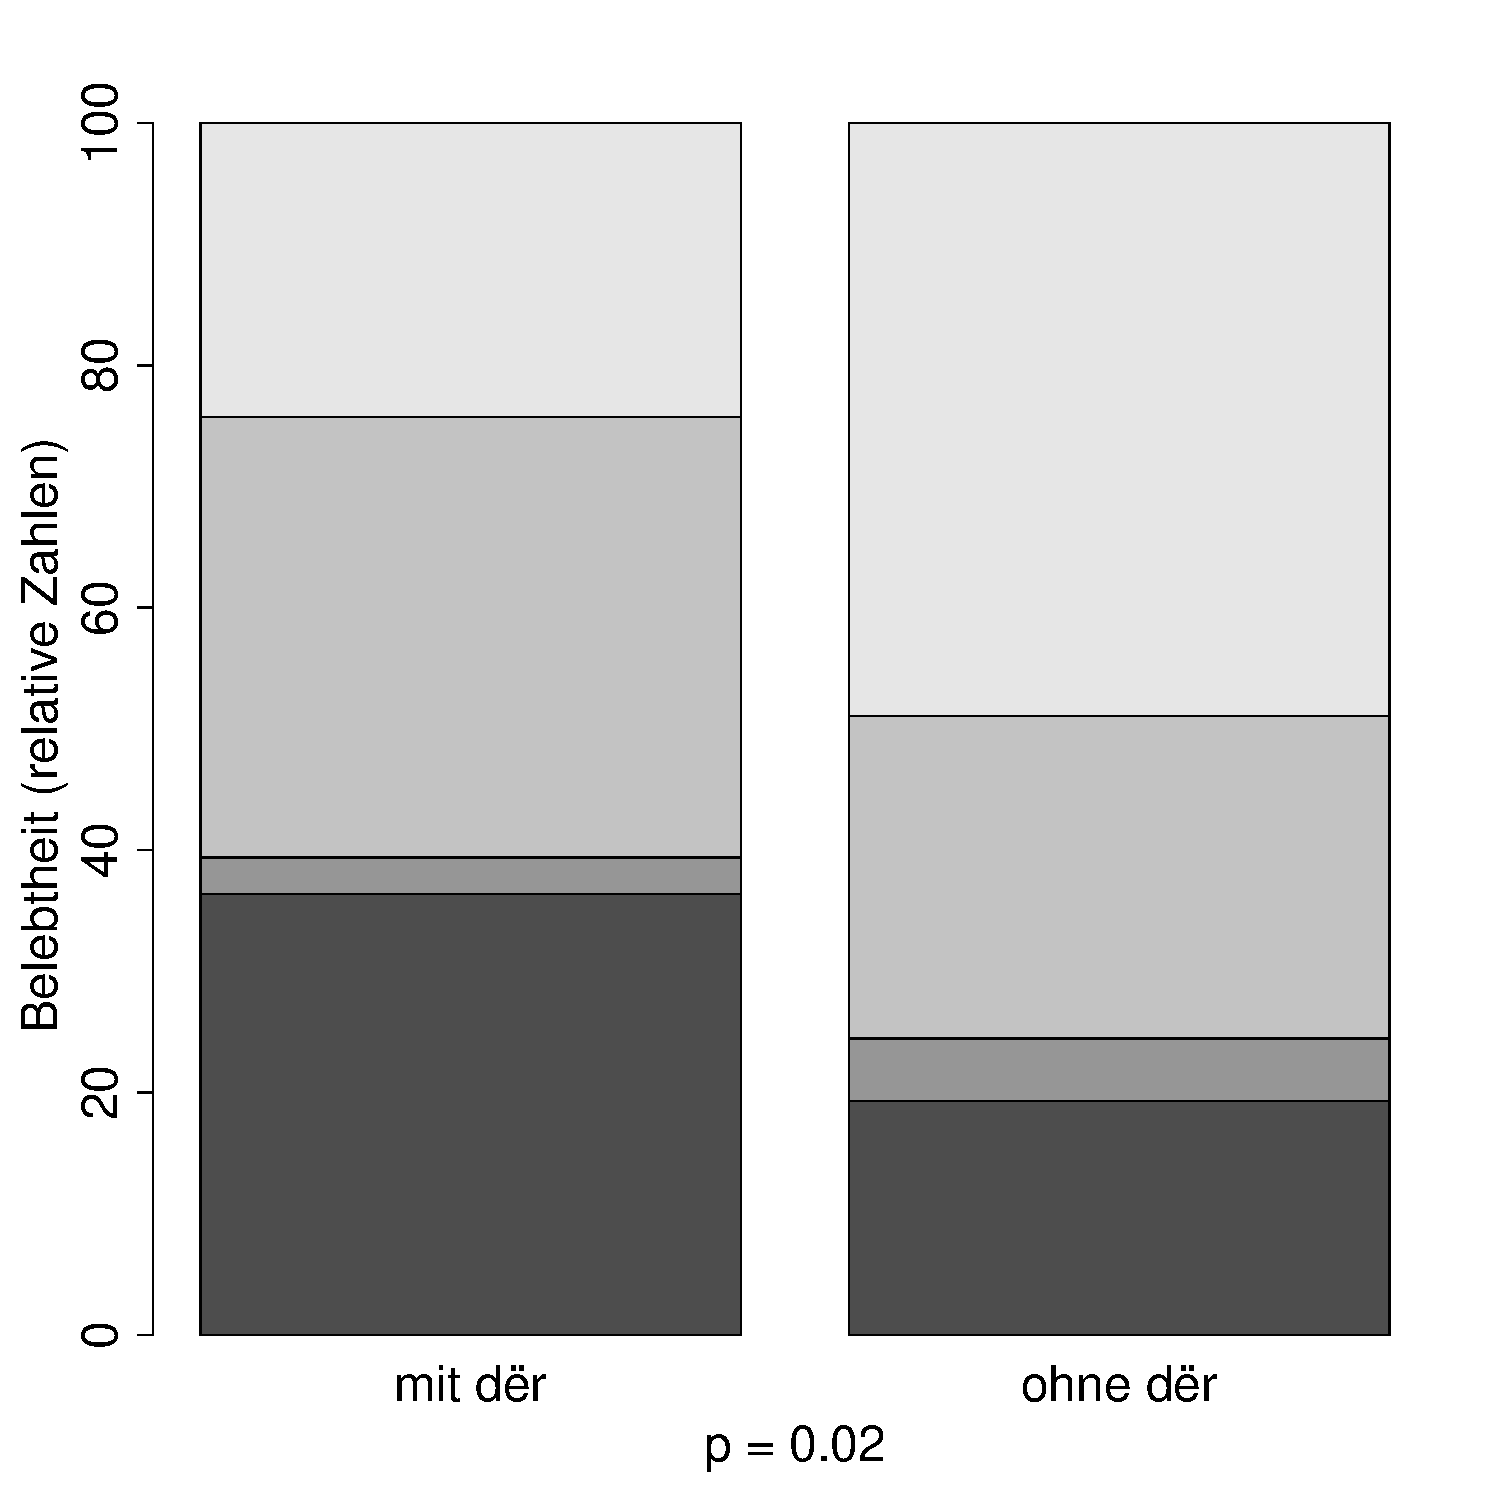
\includegraphics[height=.25\textheight]{generated/images/belebtheit-hapaxe-T}
\caption {Tatian}
\end{subfigure}%
\begin{subfigure}[b]{.5\linewidth}
  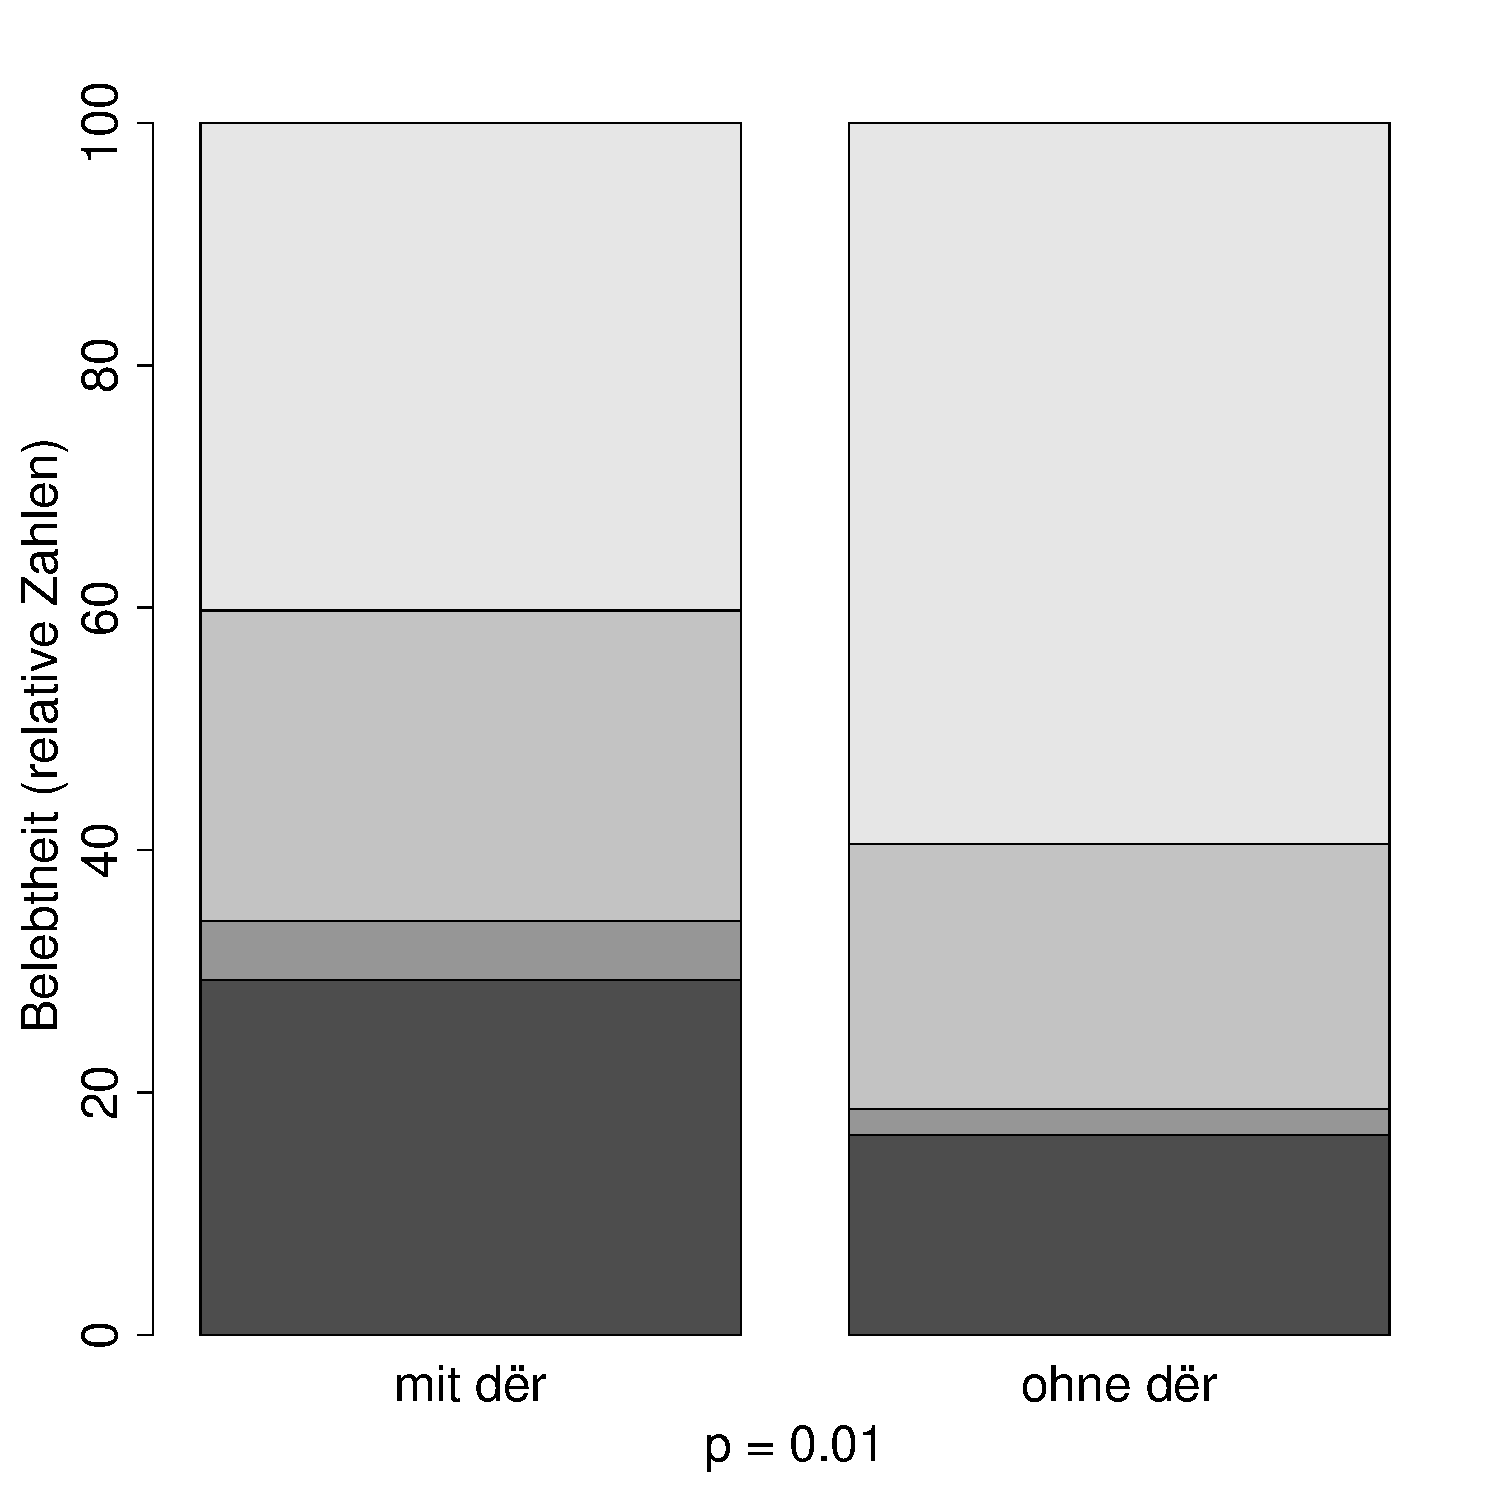
\includegraphics[height=.25\textheight]{generated/images/belebtheit-hapaxe-O}
\caption {Otfrid}
\end{subfigure}

\begin{subfigure}[b]{.5\linewidth}
  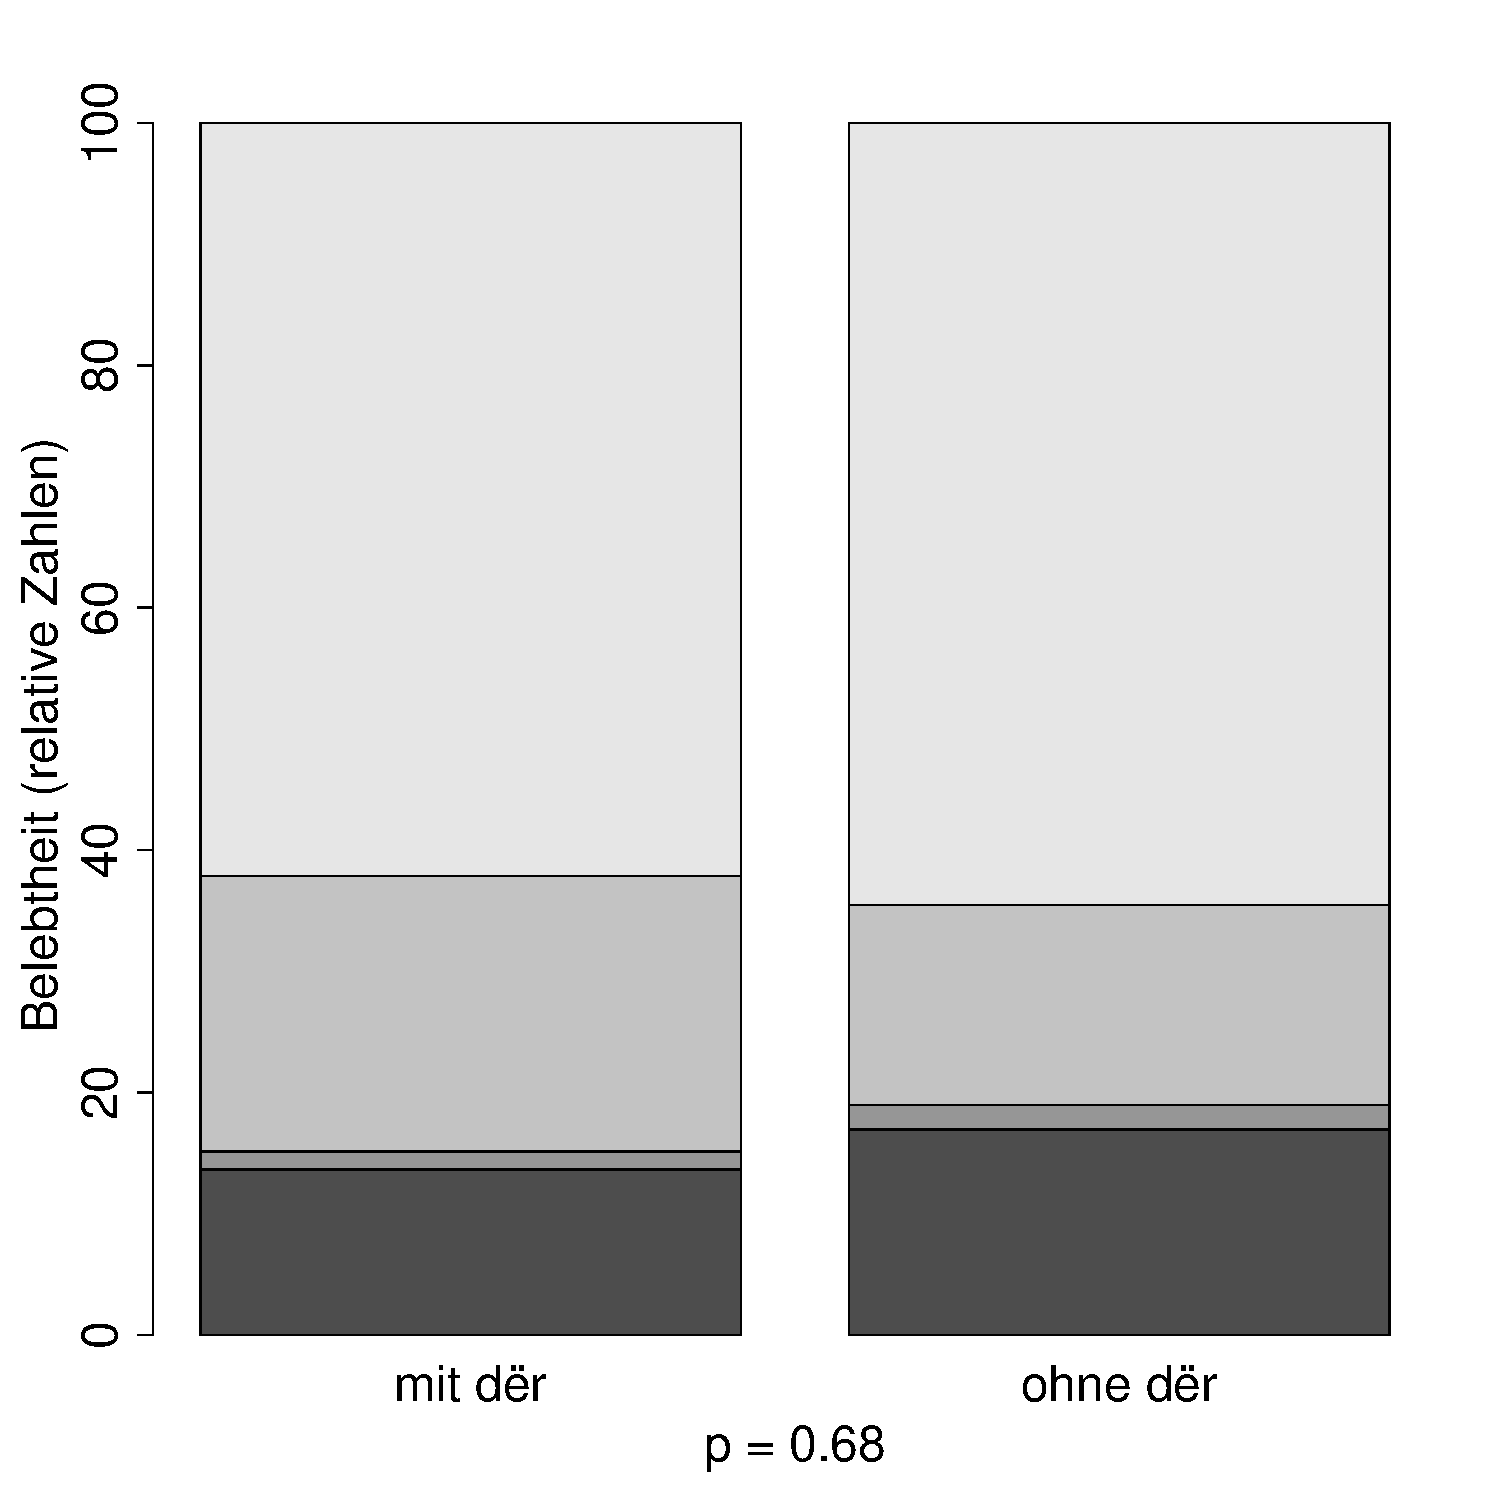
\includegraphics[height=.25\textheight]{generated/images/belebtheit-hapaxe-N}
\caption {Notker}
\end{subfigure}%
\begin{subfigure}[b]{.5\linewidth}
  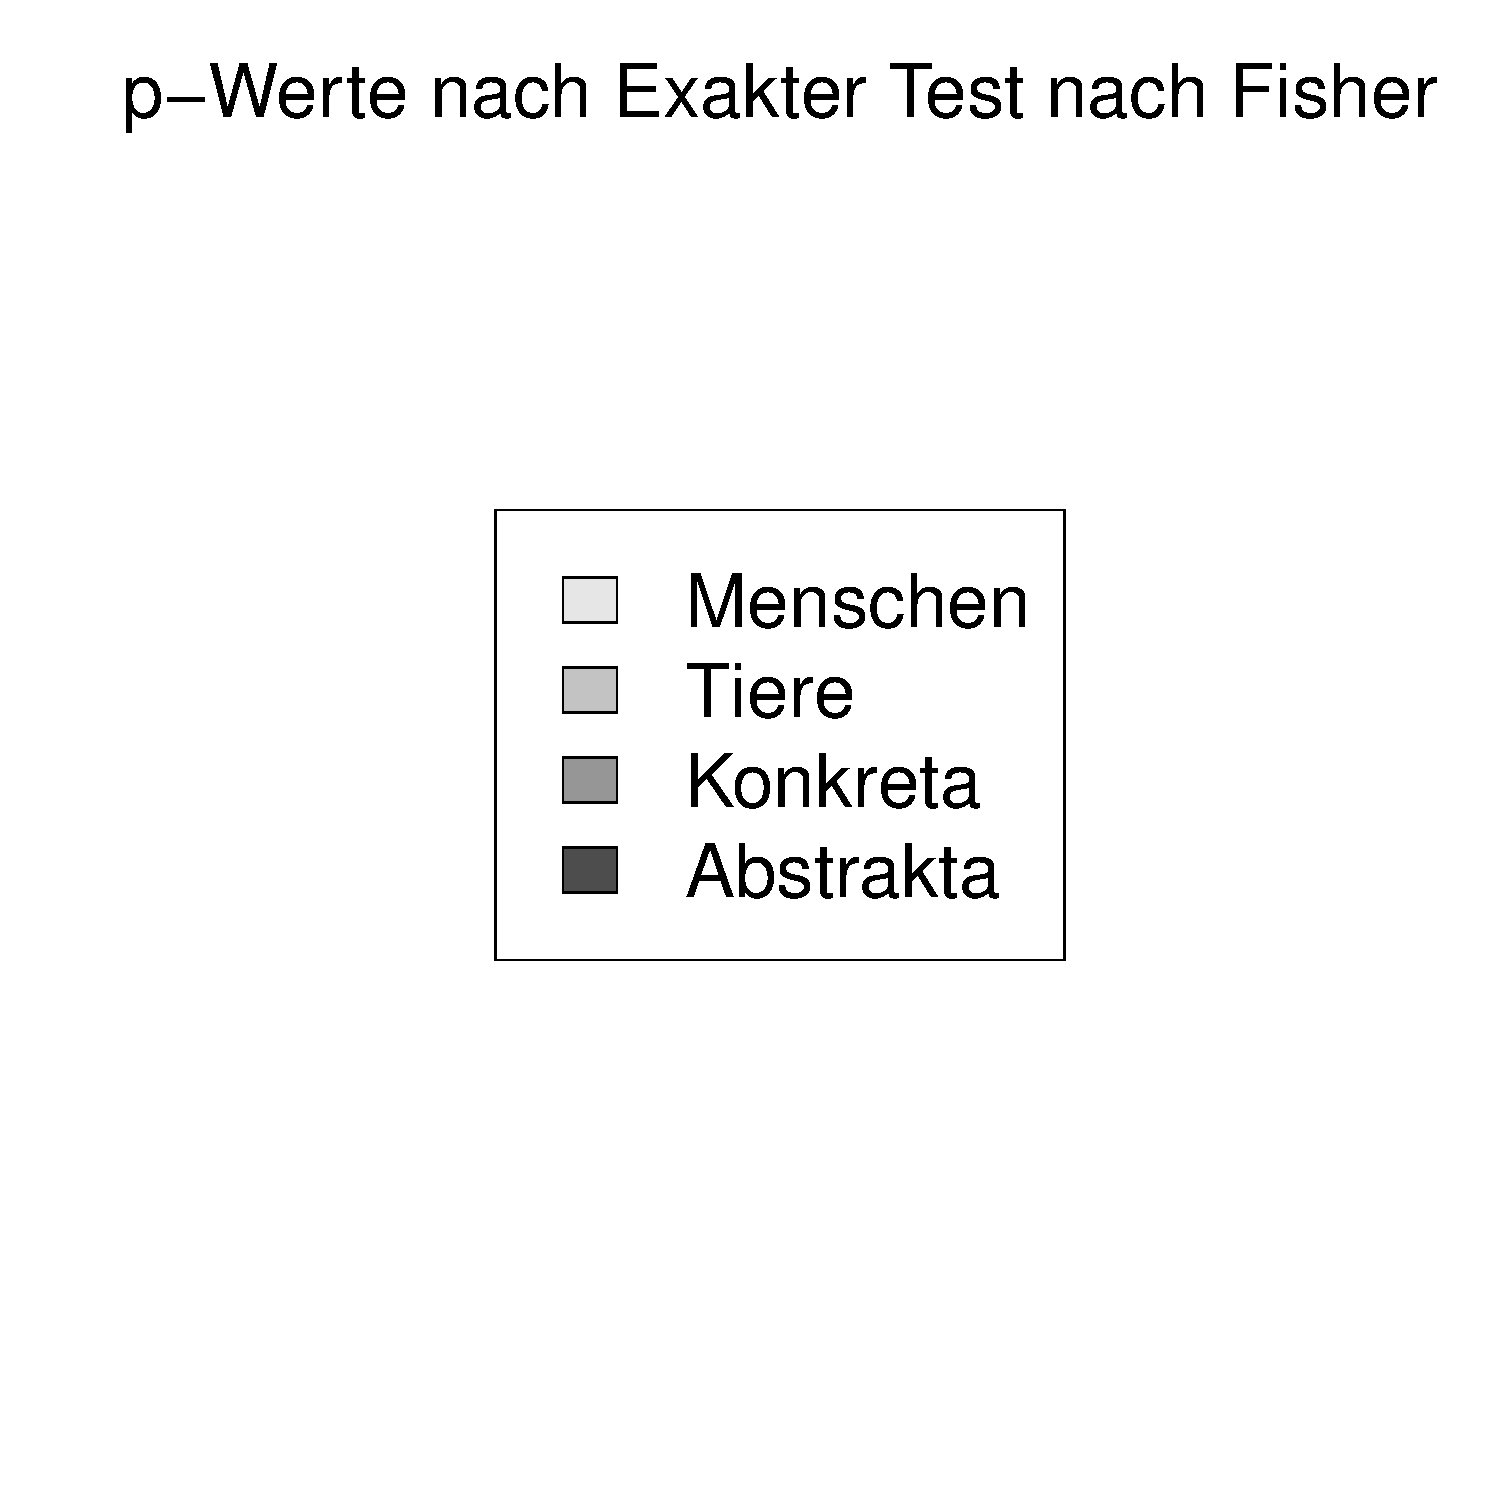
\includegraphics[height=.25\textheight]{generated/images/belebtheit-legende}
\end{subfigure}
\caption{Gebrauch von \object{dër} in Korrelation mit Belebtheit bei Hapax Legomena}\label{fig:bel-hapaxe}
\label{fig:residuals-bel-hapaxe}
\end{figure}

%\inputtable{generated/tables/bel.abs-hapaxe-I}{Gebrauch von \object{dër} in Korrelation mit Belebtheit bei Hapax Legomena; \\Isidor, absolute Zahlen}{tab:hapaxe-I}
%\inputtable{generated/tables/bel.abs-hapaxe-M}{Gebrauch von \object{dër} in Korrelation mit Belebtheit bei Hapax Legomena; \\Monseer Matthäus, absolute Zahlen}{tab:hapaxe-M}
%\inputtable{generated/tables/bel.abs-hapaxe-T}{Gebrauch von \object{dër} in Korrelation mit Belebtheit bei Hapax Legomena; \\Tatian, absolute Zahlen}{tab:hapaxe-T}
%\inputtable{generated/tables/bel.abs-hapaxe-O}{Gebrauch von \object{dër} in Korrelation mit Belebtheit bei Hapax Legomena; \\Otfrid, absolute Zahlen}{tab:hapaxe-O}
%\enlargethispage{1ex}
%\inputtable{generated/tables/bel.abs-hapaxe-N}{Gebrauch von \object{dër} in Korrelation mit Belebtheit bei Hapax Legomena; \\Notker, absolute Zahlen}{tab:hapaxe-N}



\begin{table}
\begin{tabular}{lrrrrrr}
  \lsptoprule
{Text} & {Struktur} & {Menschen} & {Tiere} & {Konkreta} & {Abstrakta} & {Summe} \\  
  \midrule
I & mit \object{dër} & 5 & 1 & 1 & 14 & 21 \\ 
 & ohne \object{dër} & 16 & 7 & 17 & 72 & 112 \\ 
 & Summe & 21 & 8 & 18 & 86 & 133 \\ 
   \midrule
M & mit \object{dër} & 6 & 0 & 5 & 6 & 17 \\ 
 & ohne \object{dër} & 15 & 5 & 27 & 51 & 98 \\ 
 & Summe & 21 & 5 & 32 & 57 & 115 \\ 
  \midrule
T & mit \object{dër} & 12 & 1 & 12 & 8 & 33 \\ 
 & ohne \object{dër} & 45 & 12 & 62 & 114 & 233 \\ 
 & Summe & 57 & 13 & 74 & 122 & 266 \\ 
  \midrule
O & mit \object{dër} & 24 & 4 & 21 & 33 & 82 \\ 
 & ohne \object{dër} & 46 & 6 & 61 & 166 & 279 \\ 
 & Summe & 70 & 10 & 82 & 199 & 361 \\ 
  \midrule
N & mit \object{dër} & 9 & 1 & 15 & 41 & 66 \\ 
 & ohne \object{dër} & 42 & 5 & 41 & 160 & 248 \\ 
 & Summe & 51 & 6 & 56 & 201 & 314 \\ 
   \lspbottomrule
\end{tabular}
\caption{Gebrauch von \object{dër} in Korrelation mit \isi{Belebtheit} bei Hapax Legomena (absolute Zahlen)}
\label{tab:hapaxe}
\end{table}

% Residuals Hapaxe

\begin{figure}
\begin{subfigure}[b]{.5\linewidth}
  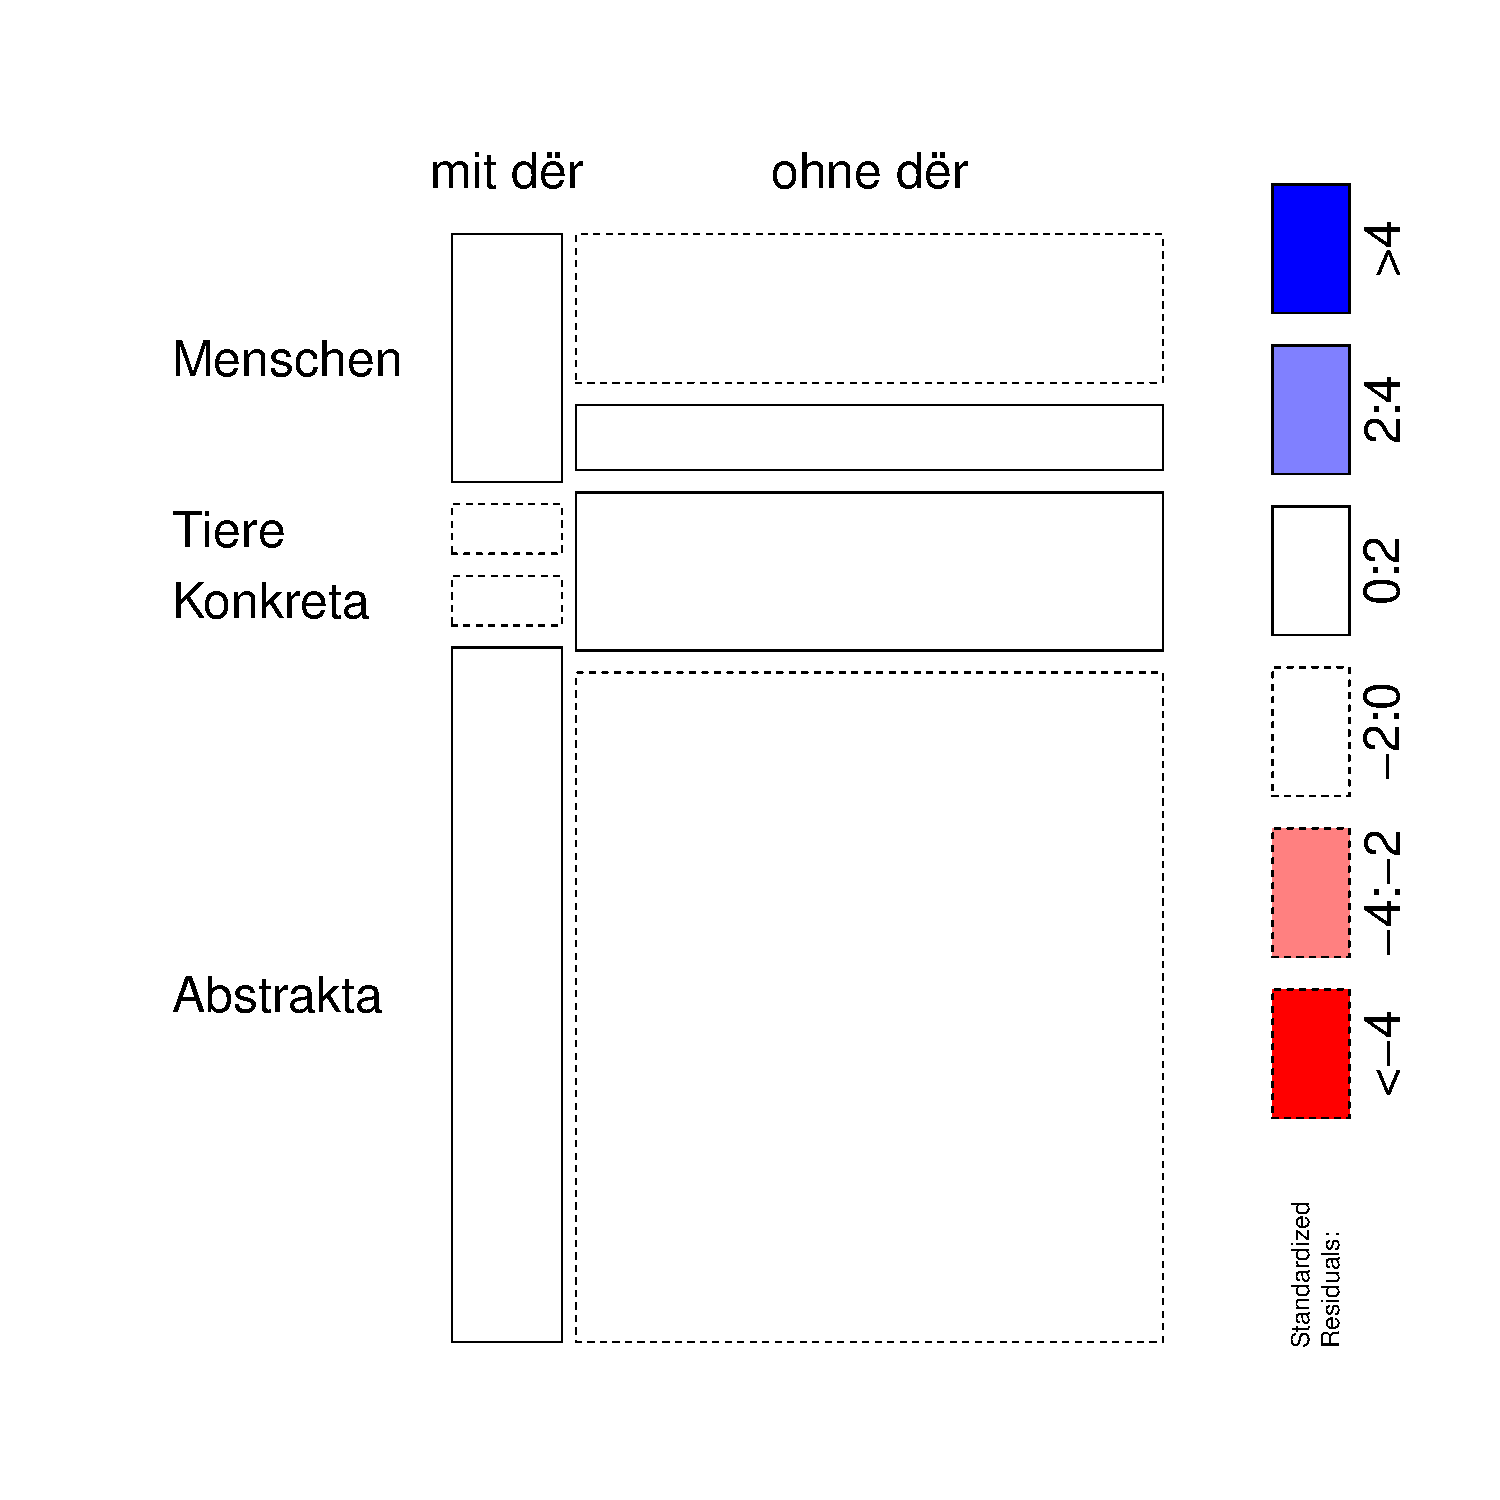
\includegraphics[height=.25\textheight]{generated/images/bel-hapaxe-residuals-I}
\caption {Isidor}
\end{subfigure}%
\begin{subfigure}[b]{.5\linewidth}
  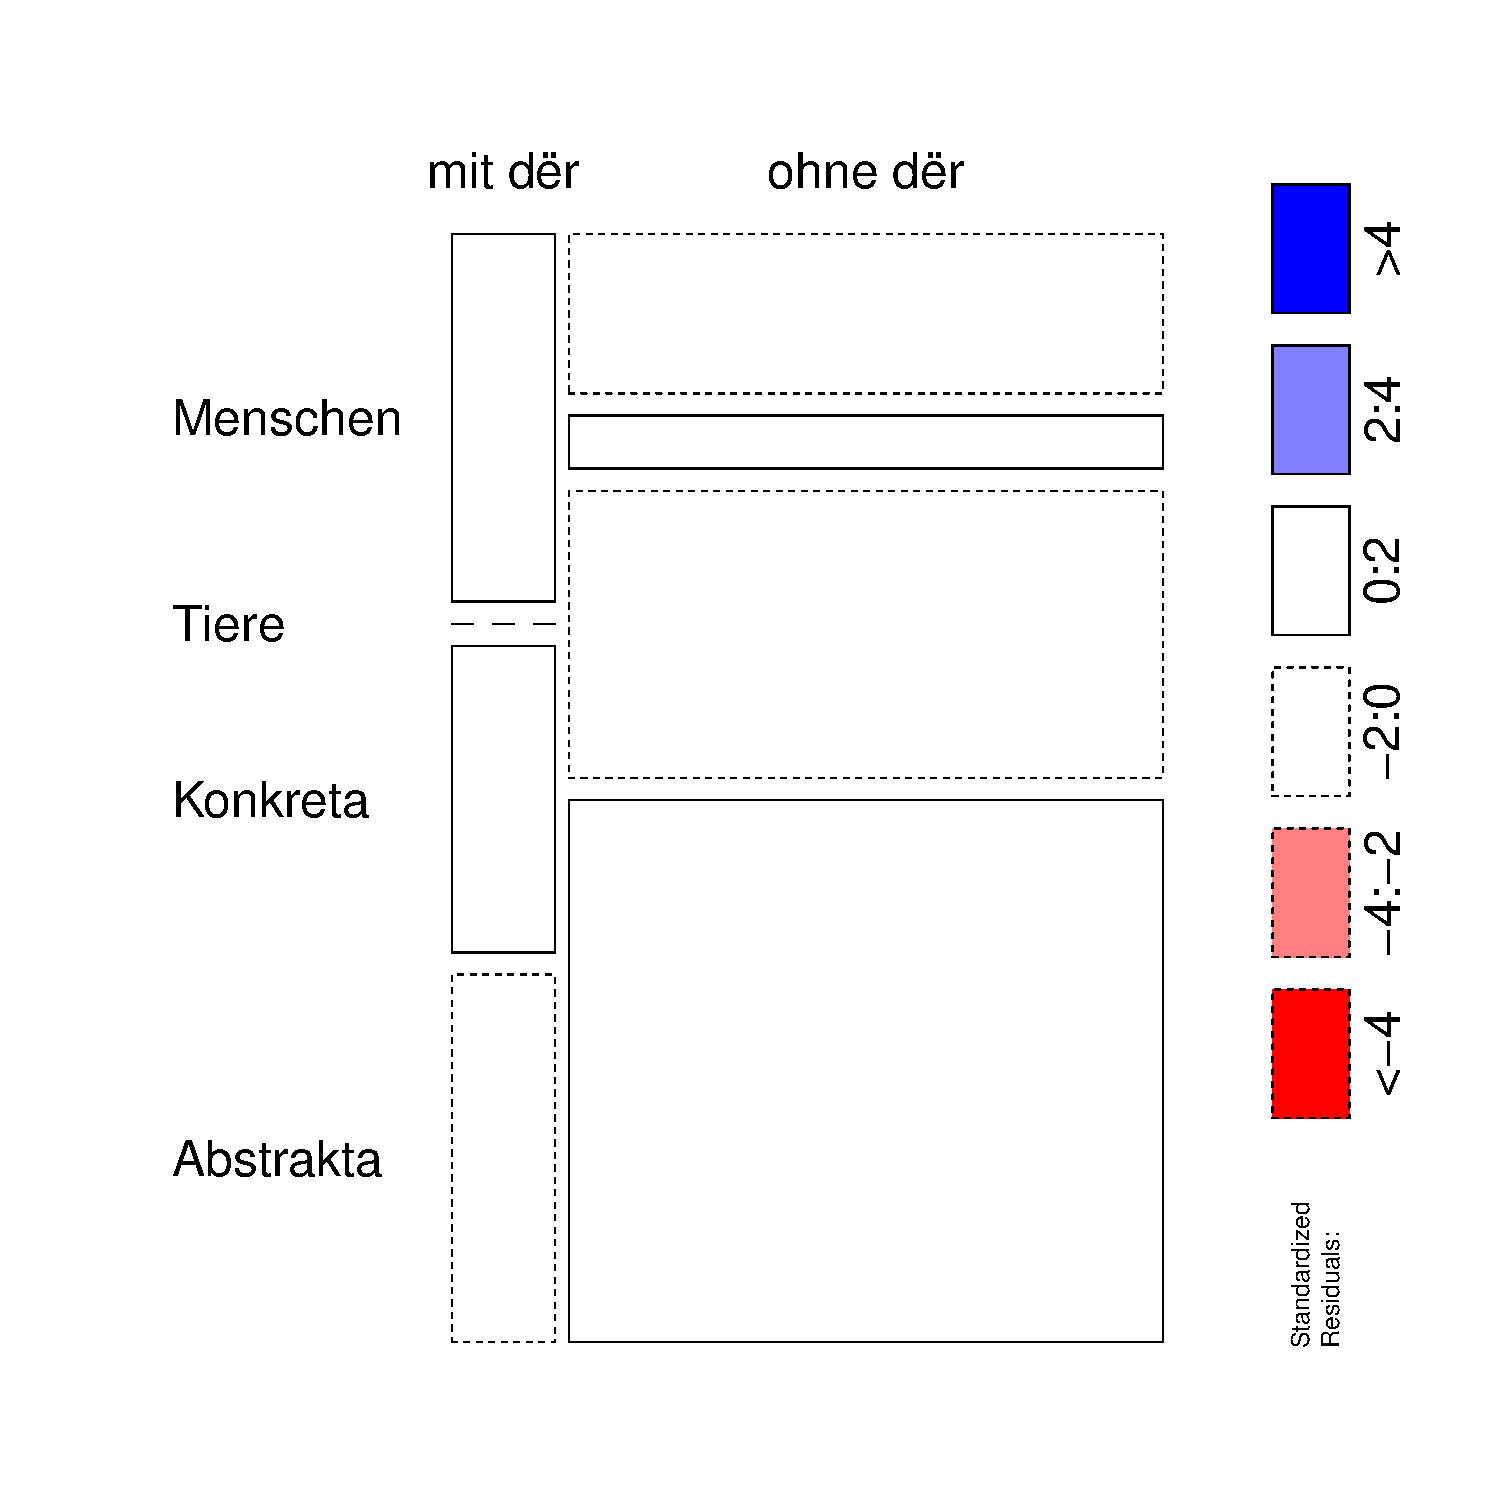
\includegraphics[height=.25\textheight]{generated/images/bel-hapaxe-residuals-M}
\caption {Monseer Matthäus}
\end{subfigure}

\begin{subfigure}[b]{.5\linewidth}
  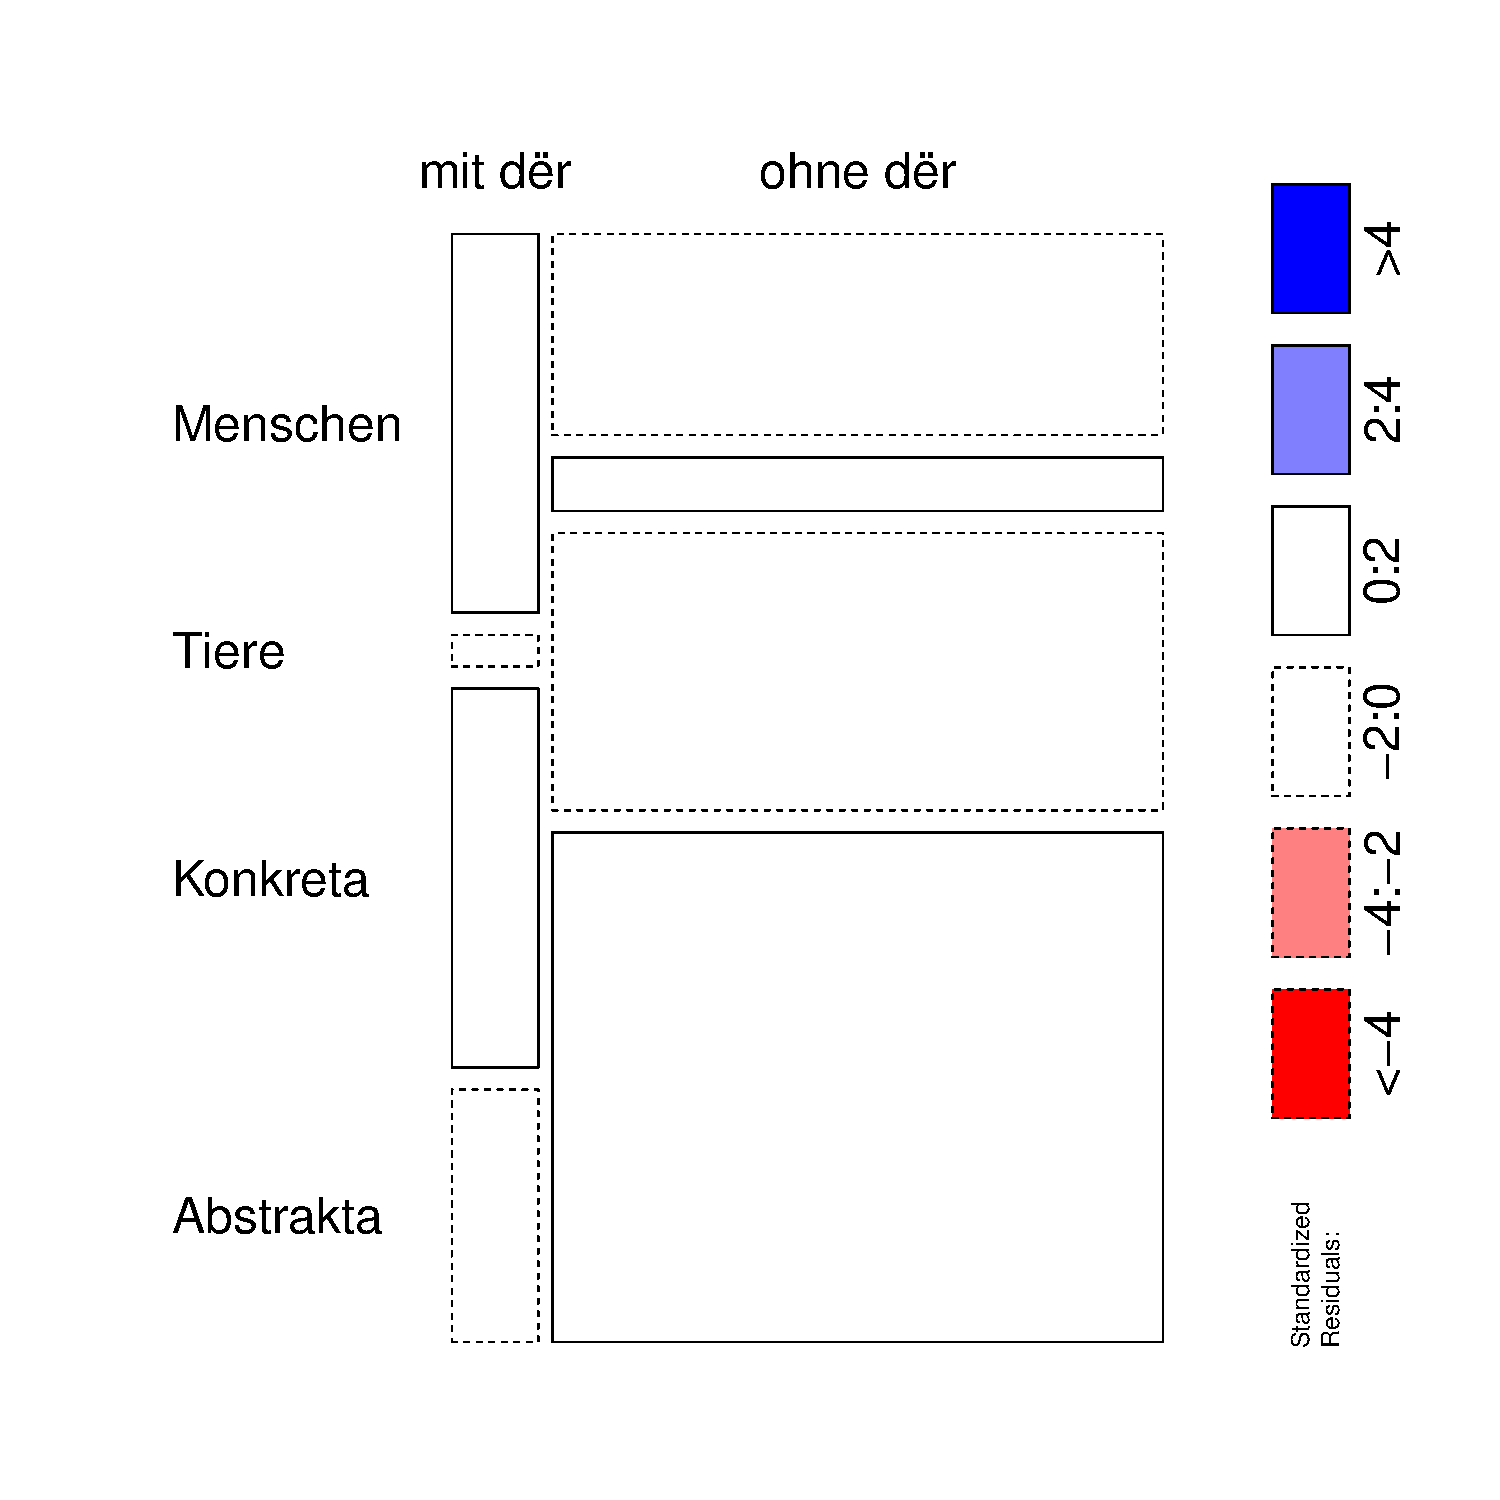
\includegraphics[height=.25\textheight]{generated/images/bel-hapaxe-residuals-T}
\caption {Tatian}
\end{subfigure}%
\begin{subfigure}[b]{.5\linewidth}
  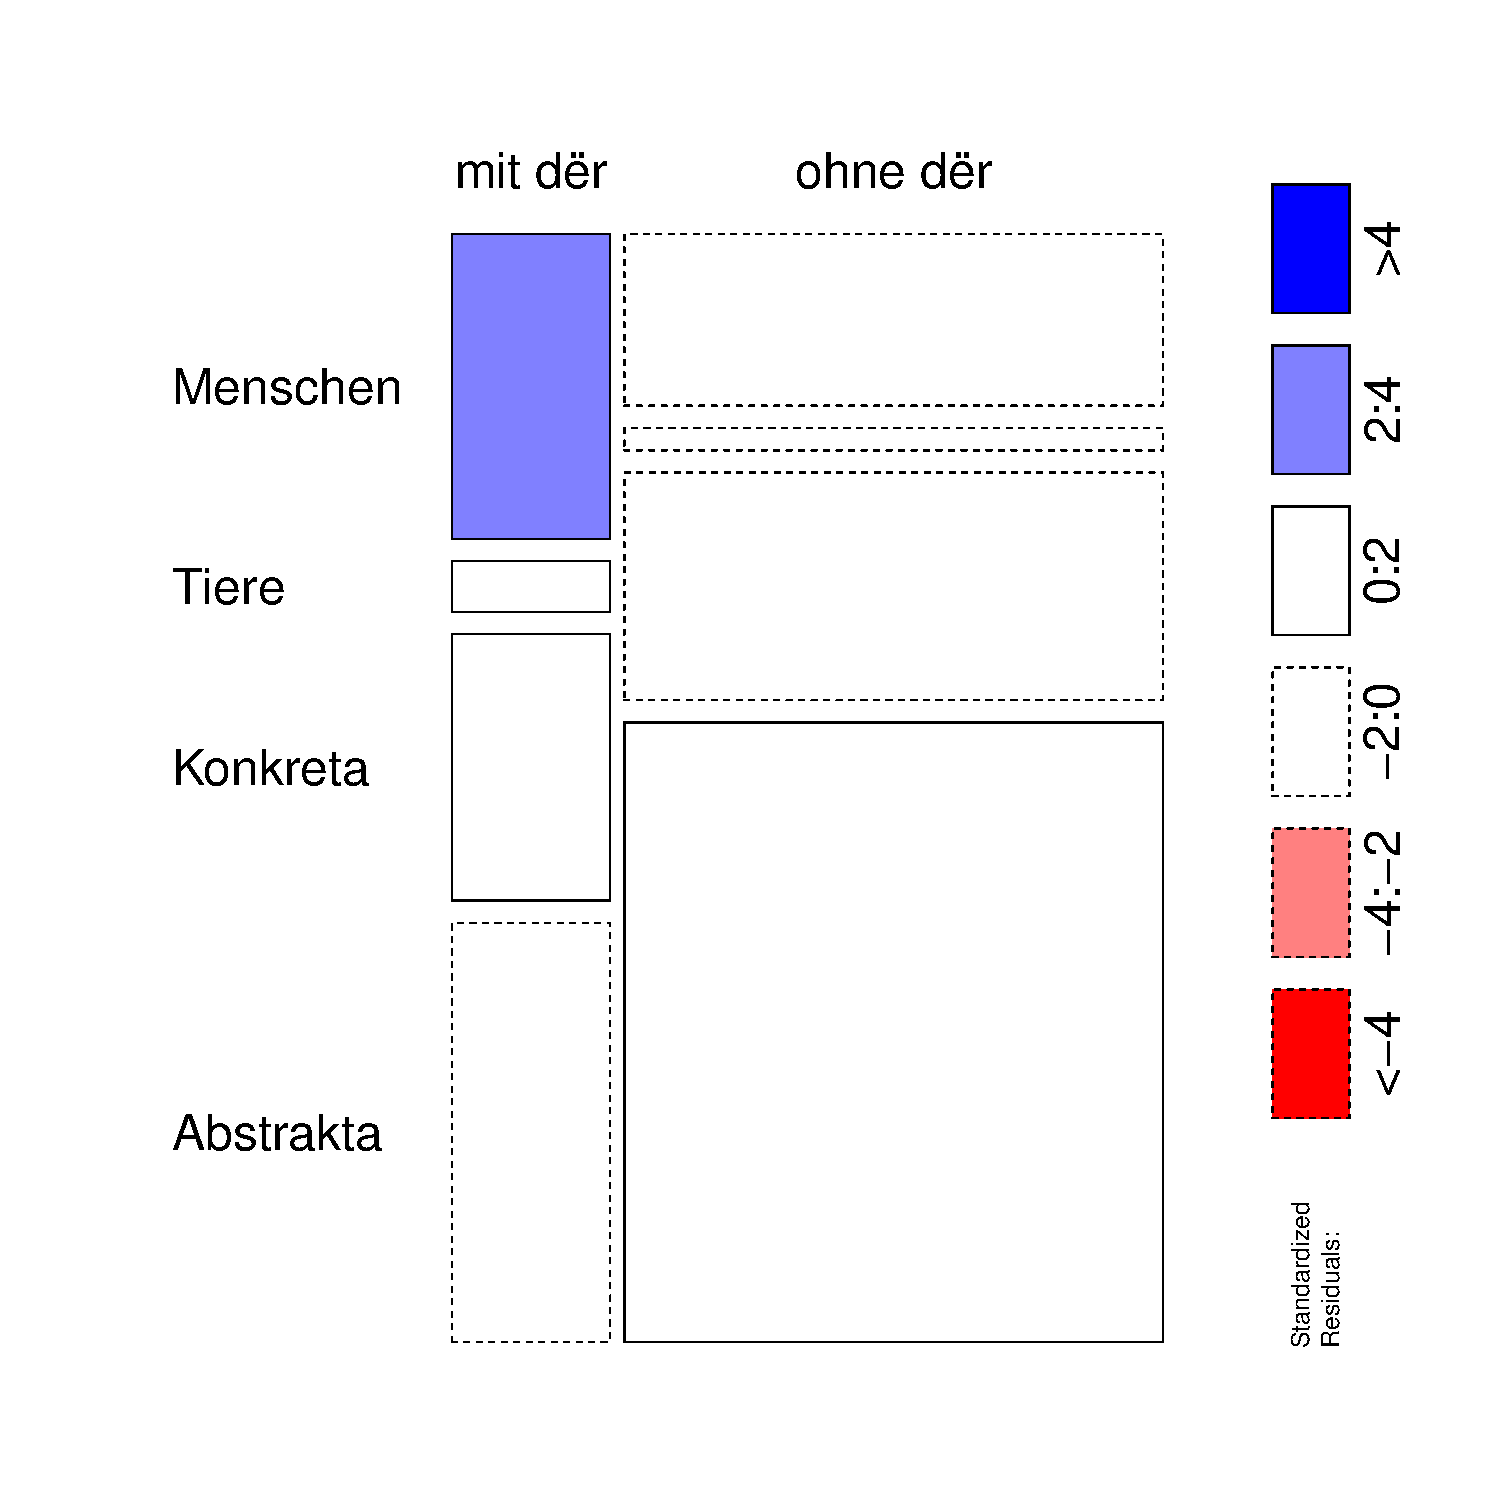
\includegraphics[height=.25\textheight]{generated/images/bel-hapaxe-residuals-O}
\caption {Otfrid}
\end{subfigure}

\begin{subfigure}[b]{.5\linewidth}
  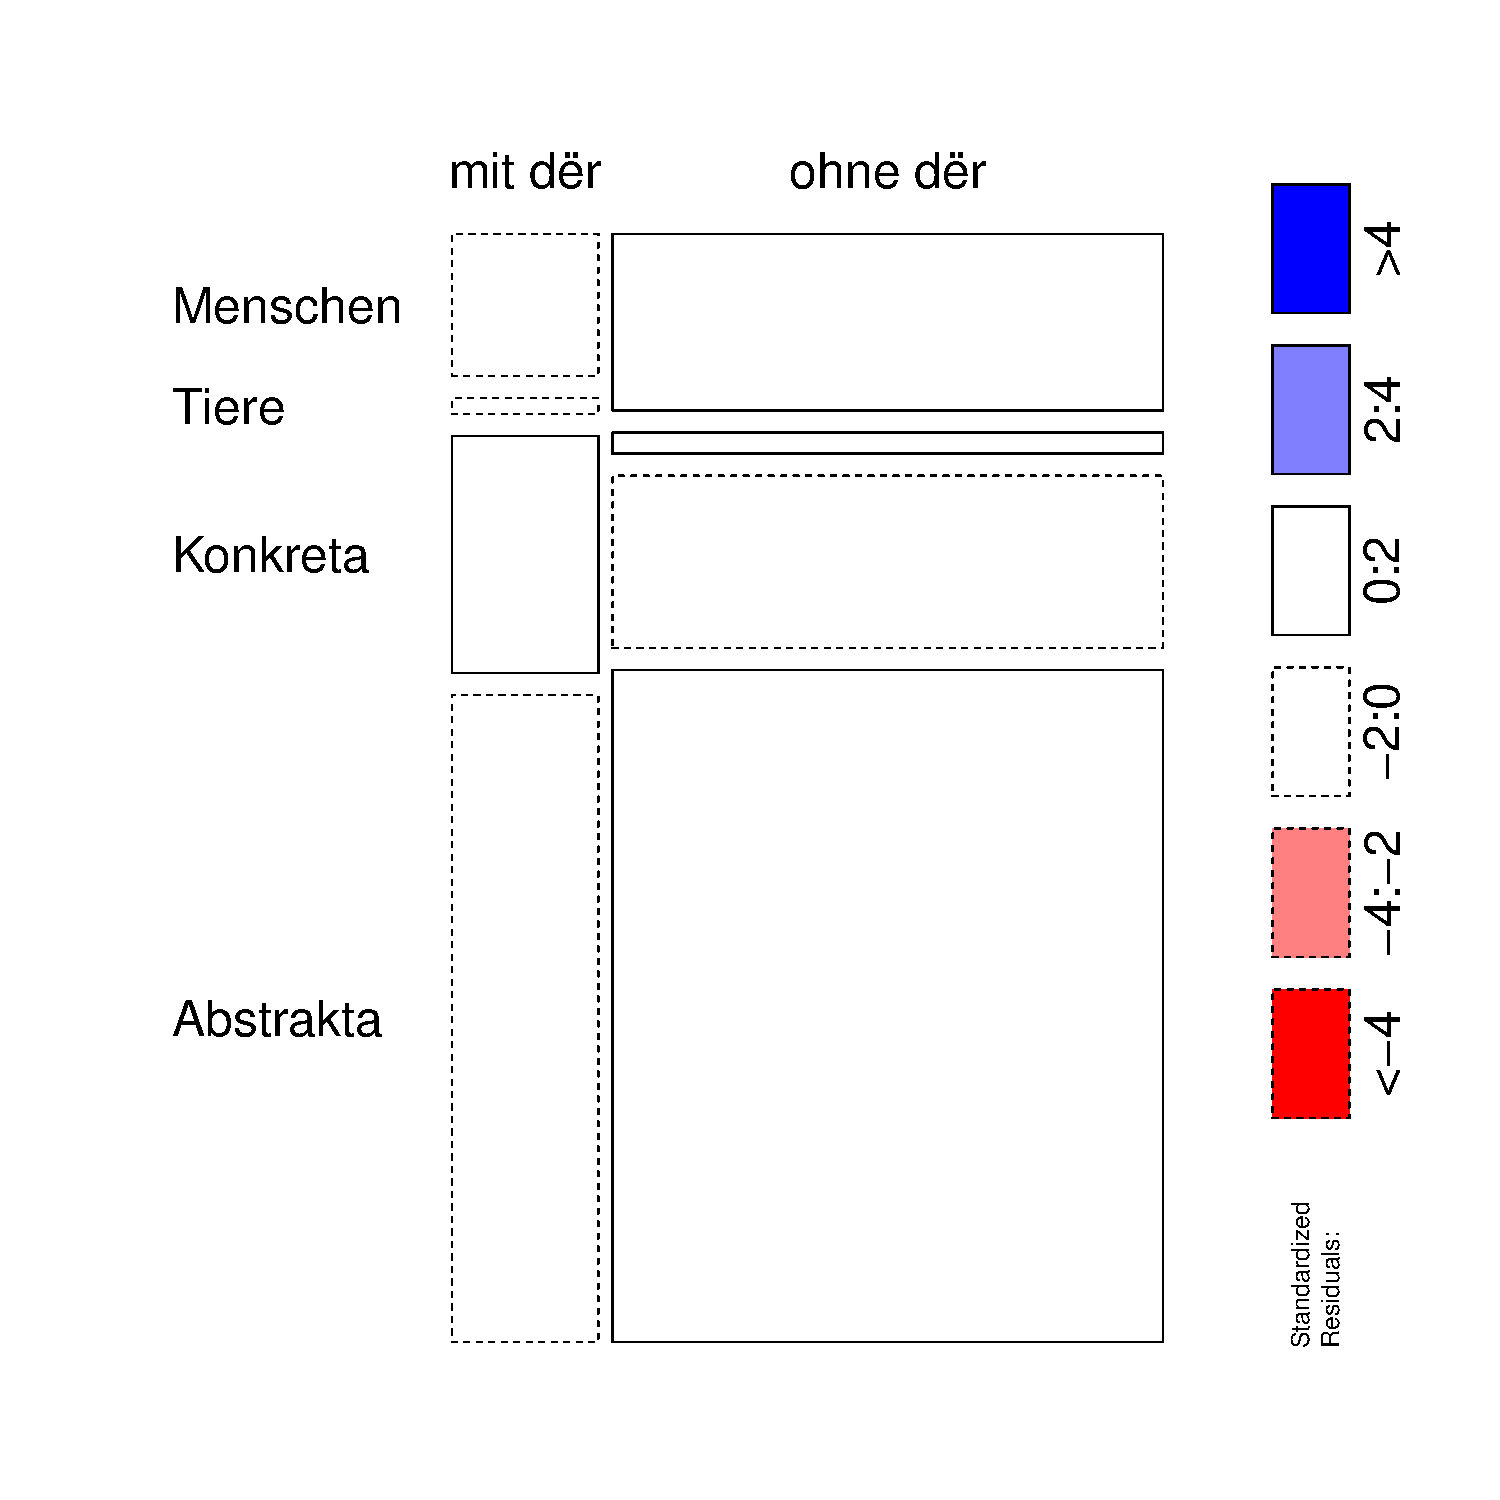
\includegraphics[height=.25\textheight]{generated/images/bel-hapaxe-residuals-N}
\caption {Notker}
\end{subfigure}
\caption{Einfluss von \isi{Belebtheit} auf \object{dër}-Gebrauch bei Hapax Legomena (Residuen)}
\label{fig:bel-hapaxe-residuals}
\end{figure}

%\subsubsection{Subkategorien Konkreta: Körperteile und Orte}
Eine weitere wichtige Gruppe, die im Rahmen der Belebtheitsannotation \is{Belebtheit}\is{Annotation}untersucht wurde, sind Körperteile. Sie sind auf der Belebtheitsskala \is{Belebtheitshierarchie} höher zu verorten als andere \is{Konkretum} Konkreta, da sie nicht veräußerbar sind und vom Menschen stärker kontrolliert werden können. Außerdem weisen sie in der Regel eine eindeutige Referenz \is{Referentialität} auf, so dass sie semantische Definita \is{Semantische Definita} repräsentieren (s.  Abschnitt~\ref{sec:pragsem}). Deshalb kann der emergierende Artikel erst nach dem Verlust seiner demonstrativen Funktion in die Domäne der Körperteile eindringen (vgl. hierzu auch Abschnitt~\ref{sec:schema}). Zudem existiert mit dem Possessivartikel \is{Possessivum} bereits ein \isi{Determinierer}, der den pränominalen Slot besetzt, und Besitzverhältnisse bzw. die Zugehörigkeit von Körperteilen zum Körper anzeigen kann. Es ist deswegen zu erwarten, dass Belege mit \object{dër} hier erst in den späteren Texten zu finden sind.\largerpage[-2]

Wie an den Häufigkeiten in Abbildung~\ref{fig:bel-koerper} abzulesen ist, zeichnet sich in Otfrids Evangelienbuch und Notkers Boethius eine  Kontextexpansion \is{Expansion} von \object{dër} auf den Bereich der Körperteile ab. 
In den drei frühsten Texten kommen nur vereinzelt Phrasen mit \object{dër}\,+\,Körperteil vor: Im Isidor ist es nur ein einzelner Belege (\object{lihhamo}). Im Monseer Matthäus ist der einzige determinierte Beleg \object{bluot}. Beide Referenten sind also keine typischen Vertreter der Kategorien \hervor{Körperteile}. Im Tatian finden sich darüber hinaus auch bei typischen Körperteilen wie \object{hërza}, \object{hand},  \object{mund} und \object{ouga} einzelne Belege mit \object{dër}. Bei Otfrid und Notker machen die determinierten Fälle immerhin knapp ein Drittel der Gesamtbelege aus. Bei Otfrid sind es die Lemmata \is{Lemma} \object{brust},  \object{lihhamo},  \object{ouga} und \object{houbit}, die herausstechen, da diese mit zweistelligen Tokenwerten vertreten sind und in jedem dritten Gebrauch determiniert werden. Alle anderen Lemmata \is{Lemma} für Körperteile bleiben in der Mehrzahl undeterminiert. Bei Notker kommt nur \object{ouga} über eine Tokenzahl von zehn -- in 4 von 14 Fällen steht es mit \object{dër}.

\begin{figure}
\begin{subfigure}[c]{.75\linewidth}
  \includegraphics[width=\linewidth]{generated/images/koerper}
\end{subfigure}%
\begin{subfigure}[c]{.2\linewidth}
  \includegraphics[width=.85\linewidth]{generated/images/ort-legende}
\end{subfigure}

\caption{Gebrauch von \object{dër} bei Bezeichnungen für Körperteile}
\label{fig:bel-koerper}
\end{figure}

Eine weitere Subkategorie der Konkreta \is{Konkretum} sind Orte. Sie wurden separat annotiert, weil sie sich als typische Kandidaten für adverbiale \is{Adverbial} und damit nicht-referentielle Phrasen möglicherweise anders verhalten als die restlichen \is{Konkretum} Konkreta. Der Vergleich von Appellativa \is{Gattungsname} mit und ohne \object{dër} bei dieser Gruppe ist für die einzelnen Texte in Abbildung~\ref{fig:bel:orte} zu sehen. In allen Texten sind Phrasen von \object{dër}\,+\,Ortsangabe zu finden. In den drei ältesten Denkmälern (Isidor, Monseer Matthäus und Tatian) machen diese gut ein Viertel der Belege aus, bei Otfrid sind es fast die Hälfte und auch Notker kommt annähernd auf 25\%. Die Durchsicht der Belege ergibt, dass Orte sowohl auf konkrete Referenten verweisen (z.B. \object{hus} oder \object{burg}) als auch nicht-referentiell auftreten, etwa in der Funktion von adverbialen \is{Adverbial} Angaben in Form von PPs (vgl. auch Abschnitt \ref{sec:ergeb-partizipanten}).
Allein die Tatsache, dass ein Referent auf einen Ort verweist, reicht also nicht aus, um Rückschlüsse auf den Gebrauch von \object{dër} zu ziehen. Faktoren wie Phrasentyp und semantische Rolle \is{Semantische Rolle} müssten in zukünftigen Untersuchungen einbezogen werden.  

\begin{figure}
\begin{subfigure}[c]{.75\linewidth}
  \includegraphics[width=\linewidth]{generated/images/ort}
\end{subfigure}%
\begin{subfigure}[c]{.2\linewidth}
  \includegraphics[width=.85\linewidth]{generated/images/ort-legende}
\end{subfigure}
\caption{Gebrauch von \object{dër} bei Ortsbezeichnungen}
  \label{fig:bel:orte}
\end{figure} 

% \begin{figure}
% \begin{subfigure}[b]{.5\linewidth}
%   \includegraphics[height=.25\textheight]{generated/images/koerper-I}
% \caption {Isidor}
% \end{subfigure}%
% \begin{subfigure}[b]{.5\linewidth}
%   \includegraphics[height=.25\textheight]{generated/images/koerper-M}
% \caption {Monseer Matthäus}
% \end{subfigure}

% \begin{subfigure}[b]{.5\linewidth}
%   \includegraphics[height=.25\textheight]{generated/images/koerper-T}
% \caption {Tatian}
% \end{subfigure}%
% \begin{subfigure}[b]{.5\linewidth}
%   \includegraphics[height=.25\textheight]{generated/images/koerper-O}
% \caption {Otfrid}
% \end{subfigure}

% \begin{subfigure}[b]{.5\linewidth}
%   \includegraphics[height=.25\textheight]{generated/images/koerper-N}
% \caption {Notker}
% \end{subfigure}%
% \begin{subfigure}[b]{.5\linewidth}
%   \includegraphics[height=.25\textheight]{generated/images/ort-legende}
% \end{subfigure}
% \caption{Gebrauch von \object{dër} bei Bezeichnungen für Körperteile}
% \label{fig:bel-koerper}
% \end{figure}

% %
%  \begin{figure}
% \begin{subfigure}[b]{.5\linewidth}
%   \includegraphics[height=.25\textheight]{generated/images/ort-I}
% \caption {Isidor}
% \end{subfigure}%
% \begin{subfigure}[b]{.5\linewidth}
%   \includegraphics[height=.25\textheight]{generated/images/ort-M}
% \caption {Monseer Matthäus}
% \end{subfigure}

% \begin{subfigure}[b]{.5\linewidth}
%   \includegraphics[width=6cm]{generated/images/ort-T}
% \caption {Tatian}
% \end{subfigure}%
% \begin{subfigure}[b]{.5\linewidth}
%   \includegraphics[height=.25\textheight]{generated/images/ort-O}
% \caption {Otfrid}
% \end{subfigure}

% \begin{subfigure}[b]{.5\linewidth}
%   \includegraphics[height=.25\textheight]{generated/images/ort-N}
% \caption {Notker}
% \end{subfigure}%
% \begin{subfigure}[b]{.5\linewidth}
%   \includegraphics[height=.25\textheight]{generated/images/ort-legende}
% \end{subfigure}
% \caption{Gebrauch von \object{dër} bei Ortsbezeichnungen}
% \label{fig:bel:orte}
% \end{figure}

\subsection{Individualität}\label{sec:ergeb-individualität}

Im Theorieteil der Arbeit (Abschnitt \ref{sec:indi}) wurden Parameter präsentiert, die die  \isi{Individualität} determinieren. Neben der Materialität (konkret vs. abstrakt), ist es die Zählbarkeit, welche dafür sorgt, dass ein Referent als distinktive Einheit wahrgenommen wird. Kontinuativa \is{Massennomen} (=\,Massennomen und Kollektiva) sind entsprechend weniger individualisiert als abgrenzbare pluralisierbare Einheiten.\linebreak Das Gleiche gilt für Referenten, die im Plural (also als Gruppe) erscheinen. Die nachfolgenden Ergebnisse zeigen erstens, inwiefern \object{dër} in den einzelnen Texten mit Kontinuativa kompatibel ist, und zweitens, ob sich signifikante Unterschiede zwischen Singular- und Pluralformen attestieren lassen.

%\subsubsection{Kontinuativa}

Analog zum Vorgehen bei den Unika \is{Unikum} (Abschnitt \ref{sec:ergeb-monosem}) wurde in allen Texten nach Lemmata \is{Lemma} gesucht, die typische Vertreter der zu untersuchenden Kategorie Kontinuativa repräsentieren. Um die Variable \isi{Belebtheit} auszublenden, wurden keine Kollektiva, sondern nur unbelebte Kontinuativa \is{Massennomen} ausgewählt. Die Auswahl ist dadurch begründet, dass die Nicht-Zählbarkeit von belebten Referenten offenbar nur wenig Einfluss auf die Determination hat. Dies verdeutlichen Kollektiva \is{Massennomen} wie \object{managi}, \object{folk} und  \object{liut}. Sie treten auch in den frühen Texten häufiger mit \object{dër} auf als ohne, vgl. die Lemmalisten \is{Lemma} in Abschnitt \ref{sec:ergeb-relevanz}. 

Um eine Vergleichbarkeit zwischen den Texten zu gewährleisten, wurde darauf geachtet, dass die Lemmata \is{Lemma} mit einer Tokenfrequenz \is{Token} von über 10 im Gesamtkorpus \is{Korpus} auftreten. Auf Basis der Untersuchungen von \textcite[28--29]{Graf1905}, \textcite[27--28]{Bell1907} und  \textcite[464]{Oubouzar1989} wurden die Lemmata \is{Lemma} \object{waʒʒar} \extrans{Wasser}, \object{gold} \extrans{Gold} und  \object{bluot} \extrans{Blut} ausgewählt; als Kontrolllemma \is{Lemma} dient das zählbare Nomen \object{stein} \extrans{Stein}. 

Tabelle~\ref{tab:wasser} zeigt die Häufigkeiten aller \object{waʒʒar}-Phrasen \is{Phrase} aufgeteilt nach Vorkommen mit und ohne \object{dër}. 

\begin{table}
\centering
\begin{tabular}{lrr}
\lsptoprule
{Text}  & {mit \object{dër}} & {ohne \object{dër}}  \\ \midrule
Isidor (790)           & 1  & 4     \\
Monseer Matthäus (810) & 0  & 0     \\
Tatian (840)           & 5  & 16    \\
Otfrid (870)           & 10 & 13    \\
Notker (1025)          & 2  & 4     \\ \lspbottomrule
\end{tabular}
\caption{\object{dër}-Setzung bei \object{waʒʒar} \extrans{Wassser}}
\label{tab:wasser}
\end{table}

Wie man sieht, dominieren in allen Texten die undeterminierten Belege. Die einzelne \object{dër}-Phrase \is{Phrase} im Isidor (\object{dhazs ir oba dhem uuazsserum suueiboda}, I 4,4) bezieht sich auf ein kurz zuvor genanntes Bibelzitat (\object{endi gotes gheist suueiboda oba uuazsserum}, I 4,4) und kann daher als eine pragmatisch motivierte Anapher \is{anaphorisch}\is{Pragmatische Definita}betrachtet werden \parencite[vgl. auch][110]{Oubouzar1989}. Aber auch eine abstrakt-situative \is{abstrakt-situativ} Lesart (\extrans{über das Wasser/Meer}) ist hier nicht auszuschließen.\largerpage[-1]

%, vgl. \REF{ex:I2244}.  
%\begin{exe}
\ex \label{ex:I2244} \gll \object{In dhiu} \object{auh} \object{dhanne} \object{0} \object{dhazs} \object{ir} \object{oba} \object{\underline{dhem}} \object{uuazsserum} \object{suueiboda} \object{0} \object{dhen} \object{heilegun} \object{gheist} \object{dhar} \object{bauhnida} \object{. } \\
{dabei} {auch} {damals} {} {dass} {er} {auf} {der} {Wasser} {sich bewegen} {} {der} {heilig} {Geist} {da} {zeigen} {}\\
\glt TODO: nhd. Übersetzung (I.4,4)
\end{exe}


Die Durchsicht der einzelnen Belege lässt vermuten,  dass  \object{dër}  eher gebraucht wird, wenn \object{waʒʒar} ein konkretes Gewässer, etwa das Meer oder einen Fluss denotiert. Ausgehend von den kontextsensitiven Übersetzungen im \isi{Korpus} steht \extrans{Wasser} für 9 determinierte und 23 undeterminierte Token. Wird \object{waʒʒar} zusätzlich mit \extrans{Meer}, \extrans{Fluss} oder \extrans{Bach} übersetzt, so verschiebt sich das Verhältnis leicht: 9 zu 14. Allerdings ist dieser Unterschied nicht signifikant (Exakter Test nach Fisher: $p=0{,}56$). Den Analysen von \textcite[464]{Oubouzar1989} zufolge steht \object{dër} bei individualisierten Einheiten und fehlt, wenn eine generische Lesart vorliegt. 


Das \isi{Lemma} \object{gold} kommt überwiegend ohne definites Artikelwort vor, s. Tabelle~\ref{tab:gold}; zukünftige qualitative Analysen müssten zeigen, inwiefern auch hier generischer \is{generisch} Gebrauch vorliegt. 
   
\begin{table}
\centering
\begin{tabular}{lrr}
\lsptoprule
{Text}  & {mit \object{dër}} & {ohne \object{dër}}  \\ \midrule
Isidor (790)           & 0  & 0     \\
Monseer Matthäus (810) & 2  & 1     \\
Tatian (840)           & 1  & 3     \\
Otfrid (870)           & 0  & 5     \\
Notker (1025)          & 0  & 4     \\ \lspbottomrule
\end{tabular}
\caption{\object{dër}-Setzung bei \object{gold} \extrans{Gold}}
\label{tab:gold}
\end{table}

%Zur Illustration ist in \REF{ex:N31557} ein Beispiel aus dem jüngsten Text (Notker) aufgeführt. 
%\begin{exe}
\ex \label{ex:N31557} \gll \object{dô} \object{sie} \object{íro} \object{\underline{gólt}} \object{púten} \object{. } \\
{da} {er} {er} {Gold} {anbieten} {}\\
\glt TODO: nhd. Übersetzung (N.2,102)
\end{exe}
 

Nur im Monseer Matthäus sowie im Tatian finden sich \object{gold}-Belege mit \object{dër}. Die nachfolgenden Übersetzungsstellen zeigen besonders gut, dass die Determinierung pragmatisch \is{Pragmatische Definita} genutzt wird. Während im Monseer Matthäus ein \object{dër} gesetzt wird, um lat. \object{in aurum templi} zu übersetzen, nutzt der Tatianübersetzer eine \is{Phrase} \object{dër}-Phrase, um \object{per templum} wiederzugeben. Mit \object{dër} wird also jeweils die andere Seite des Kontrastes ausgezeichnet -- im Monseer Matthäus ist es das Gold des Tempels, das im Vordergrund steht, im Tatian der Tempel selbst. 

\begin{exe}
\ex
lat. quicumque iuraverit per templum nihil est, qui autem iuraverit in aurum templi debet 
\sn \extrans{Wer da schwört bei dem Tempel, der ist nichts, wer aber bei dem Gold des Tempels schwört, der ist schuldig.}
\begin{xlist}
\ex \label{ex:gold-M} \gll  {so huuer so} {bi} {tem ple} {suerit} {neo uuiht} {sii}, {Der} {auuar} {\textit{in}} {\textit{demo}} {\textit{tem ples}} {\textit{golde}} {suerit}  {scul dic}  {eidh}  {sii}  \\
{jeder der} {bei} {Tempel} {schwört} {nichts} {sei}, 
{der} {aber} {in} {dem} {Tempels} {Gold} {schwört} {schuldig} {Eid} {sei} (M 17,1)\\

\ex \label{ex:gold-T} \gll 
{so uuer so} {suerit} {\textit{bi}} {\textit{themo}} {\textit{temple}} {ther} {n nist} {niouuiht}, {ther} {de} {suerit} {in}  {gold} {temples} {scal} \\
{Wer} {schwört} {bei} {dem} {Tempel} {der} {nicht ist} {nichts},
{der} {da} {schwört} {in} {Gold} {Tempels} {(ist) schuldig} (T 141,14)\\
\end{xlist}
\end{exe}

Im weiteren Text wird in beiden Übersetzungen das Gold des Tempels zweimal anaphorisch \is{anaphorisch} aufgenommen und auch hier sieht man unterschiedliche Übersetzungsverfahren: Im Tatian wird die erste Anapher \is{anaphorisch} mit \object{dër} wiedergegeben (\object{uuedar ist mera, thaz gold oda templum thaz dar heilagot gold?}, T 141,14),
im Monseer Matthäus ist es die zweite (\object{huuedar ist za uuare mera  gold odo kirihha diu daz golth uuihit?}, M 17,6), sinngemäß: \extrans{Was ist mehr wert, das Gold oder die Kirche, die das Gold heiligt?}. 
%\begin{exe}
\ex \label{ex:T28605} \gll \object{ther} \object{de} \object{suerit} \object{in} \object{gold} \object{\underline{temples}}  \\
{der} {da} {schwören} {in} {Gold} {Tempel}  {}\\
\glt TODO: nhd. Übersetzung (T.141,14)
\end{exe}

%\begin{exe}
\ex \label{ex:T28617} \gll \object{Dumbe} \object{inti} \object{blinte} \object{0} \object{uuedar} \object{ist} \object{mera} \object{0} \object{thaz} \object{\underline{gold}} \object{oda} \object{templum} \object{thaz} \object{dar} \object{heilagot} \object{gold} \object{?} \\
{dumm} {und} {blind} {} {wer} {sein} {mehr} {} {der} {Gold} {oder} {Tempel} {der} {da} {heiligen} {Gold} {}\\
\glt TODO: nhd. Übersetzung (T.141,14)
\end{exe}


Interessant ist der Vergleich von \object{gold} mit einem zählbaren Referenten wie  \object{stein}, s. Tabelle~\ref{tab:stein}. Die Wahrscheinlichkeit einer \object{dër}-Setzung ist hier höher: Bei \object{gold} liegt das Verhältnis von determinierten zu undeterminierten \isi{Token} bei 3 zu 13, d.h. jedes fünfte \isi{Token} trägt ein \object{dër}; bei \object{stein} ist es mit 19 zu 34 jedes dritte. 

\begin{table}
\centering
\begin{tabular}{lrr}
\lsptoprule
{Text}  & {mit \object{dër}} & {ohne \object{dër}} \\ \midrule
Isidor (790)           & 0  & 0     \\
Monseer Matthäus (810) & 0  & 0     \\
Tatian (840)           & 7  & 21    \\
Otfrid (870)           & 10 & 12    \\
Notker (1025)          & 2  & 1     \\ \lspbottomrule
\end{tabular}
\caption{\object{dër}-Setzung bei \object{stein} \extrans{Stein}}
\label{tab:stein}
\end{table}

Die nachfolgenden Tabellen zeigen die Verteilung von \object{dër} bei \object{bluot}. Auch bei diesem \isi{Massennomen} dominiert die undeterminierte Variante. Nur bei eindeutiger Referenz \is{Referentialität} steht ein \object{dër}, so etwa im Tatian, wenn von Pilatus' Blut die Rede ist \object{thero bluot Pilatus} (T, 102,1) oder im Monseer Matthäus, wo \extrans{das gerechte Blut} mit einem \isi{Adjektiv} und einem restrinktiven Relativsatz näher spezifiziert wird: \object{al daz reht ·  uuisiga bluoth · daz ubar ærda ist ka gozan} (M, 18,20--21).

%\begin{exe}
\ex \label{ex:M3723} \gll \object{*** } \object{chauf tun} \object{mit} \object{dem} \object{***} \object{z enes} \object{*** } \object{za} \object{grabum} \object{; } \object{Bidiu} \object{ist} \object{kanemnit} \object{*** } \object{daz} \object{ist} \object{\underline{bluotes}} \object{acchar} \object{untaz} \object{hiu tu} \object{Duo} \object{uuard} \object{arfullit} \object{daz} \object{kaquetan} \object{ist} \object{durah} \object{hieremiam} \object{den} \object{fora sagun} \object{Enti} \object{ant ·\fengun} \object{drizuc} \object{pendingo} \object{*** } \object{uuerdh} \object{daz} \object{sie} \object{ghachurun} \object{fona} \object{*** } \object{gabun} \object{dea} \object{uuidar} \object{demo} \object{hauuanares} \object{*** } \object{so} \object{mir} \object{kabot} \\
{} {kaufen} {mit} {der} {} {} {} {zu} {Grab} {} {deshalb} {sein} {benennen} {} {der} {sein} {Blut} {Acker} {bis} {heute} {da} {werden} {erfüllen} {der} {sprechen} {sein} {durch} {Jeremias} {der} {Prophet} {und} {empfangen} {dreißig} {Pfenning} {} {Wert} {der} {er} {auswählen} {von} {} {geben} {der} {wider} {der} {Töpfer} {} {so} {ich} {gebieten}\\
\glt TODO: nhd. Übersetzung (M.18,NA)
\end{exe}
 

\begin{table}
\centering
\begin{tabular}{lrr}
\lsptoprule
{Text}  & {mit \object{dër}} & {ohne \object{dër}} \\ \midrule
Isidor (790)           & 0  & 0     \\
Monseer Matthäus (810) & 2  & 6     \\
Tatian (840)           & 1  & 16    \\
Otfrid (870)           & 0  & 10    \\
Notker (1025)          & 2  & 0     \\ \lspbottomrule
\end{tabular}
\caption{\object{dër}-Setzung bei \object{bluot} \extrans{Blut}}
\label{tab:blut}
\end{table}


%\subsubsection{Numerus}

Da Referenten im Singular individuierter sind als Referenten, die im Plural auftreten (vgl. Abschnitt \ref{section:mass}), wurde auch der \isi{Numerus} als Variable für \isi{Individualität}  betrachtet. In Abbildung~\ref{fig:numerus} sind alle Appellativa \is{Gattungsname} aufgeteilt nach \isi{Numerus} und \object{dër}-Gebrauch abgebildet.

\begin{figure}[p]
\begin{subfigure}[b]{.5\linewidth}
  \includegraphics[height=.25\textheight]{generated/images/numerus-isidor}
\caption {Isidor}
\end{subfigure}%
\begin{subfigure}[b]{.5\linewidth}
  \includegraphics[height=.25\textheight]{generated/images/numerus-matt}
\caption {Monseer Matthäus}
\end{subfigure}

\begin{subfigure}[b]{.5\linewidth}
  \includegraphics[height=.25\textheight]{generated/images/numerus-tatian}
\caption {Tatian}
\end{subfigure}%
\begin{subfigure}[b]{.5\linewidth}
  \includegraphics[height=.25\textheight]{generated/images/numerus-otfrid}
\caption {Otfrid}
\end{subfigure}

\begin{subfigure}[b]{.5\linewidth}
  \includegraphics[height=.25\textheight]{generated/images/numerus-notker}
\caption {Notker}
\end{subfigure}%
\begin{subfigure}[b]{.5\linewidth}
  \includegraphics[height=.25\textheight]{generated/images/numerus-legende}
\end{subfigure}

\caption{Gebrauch von \object{dër} in Korrelation mit \isi{Numerus} (relative Häufigkeiten)}
\label{fig:numerus}
\end{figure}

Man sieht, dass die Belege im Singular in allen Texten deutlich in der Überzahl sind. Sie werden aber nicht zwangsläufig häufiger als erwartet mit \object{dër} determiniert. Die Unterschiede zwischen der Singular- und Pluralverteilung wurde mit Hilfe des Exakten Tests nach Fisher auf statistische Signifikanz geprüft. Im Isidor gibt es mehr Belege im Singular, die mit \object{dër} determiniert werden als im Plural. Dieser Unterschied ist signifikant ($p=0{,}01$). Die umgekehrte Tendenz im Monseer Matthäus hält dem statistischen Test nicht stand ($p=0{,}12$). Mit einem $p$-Wert,
der jeweils kleiner als $0{,}01$ ist, muss die leichte Affinität der Singularbelege zu \object{dër} im Tatian bzw. der Pluralbelege bei Otfrid dagegen als signifikant eingestuft werden. Bei Notker ist das Verhältnis ausgeglichen ($p=1$). Die Hypothese, dass Referenten im
Singular wahrscheinlicher mit \object{dër} hervorgehoben werden als plurale
Referenten, lässt sich also mit dieser Gegenüberstellung nicht verifizieren. 

Die bisherigen Ergebnisse deuten darauf hin, dass andere Faktoren den \isi{Numerus} als Individualitätsparameter \is{Individualität} überlagern: So wurde im vorhergehenden Abschnitt gezeigt, wie \isi{Massennomen} überwiegend ohne \object{dër} vorkommen, aber typischerweise im Singular stehen. Auf der anderen Seite gibt es viele belebte und konkrete Referenten, die häufig mit \object{dër} determiniert werden, aber im Plural auftreten, darunter bspw. das bei Otfrid hochfrequente \object{liut} \extrans{Volk, Leute} oder auch ganze Völkergruppen wie die Juden oder Pharisäer.


\subsection{Relevanz}\label{sec:ergeb-relevanz}

Um eine Übersicht zu erhalten, welche Lemmata \is{Lemma} in den einzelnen Texten präferiert in Kombination mit \object{dër} (sowohl in Kontakt- als auch Distanzstellung) auftreten, wurden die Daten in zwei Gruppen eingeteilt: Die eine beinhaltet alle \is{Lemma} Lemmata, deren \isi{Token} in $\geq$ 80\% aller Fälle  mit \object{dër} determiniert werden. In der anderen sind \is{Lemma} Lemmata, deren \isi{Token} in weniger als 20\%  ein \object{dër} bei sich tragen. Dargestellt sind nachfolgend jeweils die Spitzenreiter dieser Gruppen. Aus diesen Darstellungen können Rückschlüsse auf den Faktor kulturelle bzw. thematische \isi{Relevanz} gezogen werden (vgl. Abschnitt \ref{sec:relevanz}). Alle menschlichen Referenten wurden zusätzlich nach Geschlecht annotiert. Die Frage ist, ob patriarchiale Machtverhätnisse  einen Einfluss auf die \object{dër}-Setzung haben, und ob sich dies bei der Distribution von weiblichen und männlichen Referenten widerspiegelt. Die Ergebnisse hierzu werden nachfolgend in die Diskussion der Frequenzlisten eingepflegt.\footnote{Referenten, bei denen das Geschlecht unklar ist, etwa bei \object{Bürgern}, wurden nicht mit aufgenommen.} Was die nachfolgenden Daten nicht zeigen, sind konkrete Gebrauchskontexte: Ob die Belege hinter den Zahlen z.B. in anaphorische \is{anaphorisch} oder generische \is{generisch} Kontexte eingebettet sind, müsste in zukünftigen Studien überprüft werden. \footnote{Die Kategorie \object{übermenschlich}, die im Rahmen der Belebtheitsannotation \is{Belebtheit}\is{Annotation}gekennzeichnet wurde, enthält fast ausschließlich unikale Referenten (\object{Gott, der heilige Geist, der Teufel, der Heiland}). Sie wurden bereits in Abschnitt \ref{sec:ergeb-monosem} diskutiert und werden daher an dieser Stelle nicht weiter besprochen.} 

In Tabelle~\ref {tab:lemma.mit.Isidor} sind zunächst die Top-5-Lemmata \is{Lemma}  aufgeführt, die im Isidor, also dem ältesten Text, in der Mehrheit mit \object{dër} vorkommen. 

%\subsubsection{Isidor}
%Isidor mit
\inputtable{generated/tables/lemma.top10.mit-Isidor.bearbeitet}{Lemmaliste-Top-5 mit \object{dër} in $\geq$ 80\% der Belege (Isidor) }{tab:lemma.mit.Isidor}

Man sieht, dass die Liste fast ausschließlich aus biblischen Figuren besteht -- mit \object{burg} ist Jerusalem gemeint und die \object{magad} referiert immer auf die Jungfrau Maria. Interessanterweise werden andere weibliche Referenten (\object{muoter}, \object{tohter}) nicht mit \object{dër} determiniert (insgesamt wird nur auf fünf Frauen mit Appellativa \is{Gattungsname} referiert), was als Zeichen für den Einfluss der religiösen \isi{Relevanz} gewertet werden kann. 
Die nachfolgende Tabelle nimmt die umgekehrte Perspektive ein: Bei welchen Lemmata \is{Lemma} dominiert im Text die artikellose Form? Auch hier sind es biblische Referenten. Belege mit \object{truhtin} erscheinen häufig im \isi{Vokativ}, was die \object{dër}-Resistenz erklären kann. Alle anderen sind monoreferent und/oder typische Kandidaten für generische \is{generisch} Kontexte.

%Isidor ohne
\inputtable{generated/tables/lemma.top10.ohne-Isidor.bearbeitet}{Lemmaliste-Top-5 mit \object{dër} in $<20\%$ der Belege (Isidor)}{tab:lemma.ohne.Isidor}

%\subsubsection{Monseer Matthäus}

Im Monseer Matthäus sind es gesellschaftlich wichtige Referenten, die mit hoher Tokenfrequenz auftreten und mit \object{dër} determiniert werden (\object{ewawart, herizoho, herizo}), s. Tabelle~\ref{tab:lemma.mit.Matt}. Mit \object{managi} ist die Schar gemeint, die den Taten Jesus beiwohnt. Wird mit \object{diota} hingegen auf eine abstraktere und größere Menschenmenge Bezug genommen, so bleiben diese undeterminiert (vgl. Tabelle~\ref{tab:lemma.ohne.Matt}), was dafür spricht, dass hier der Faktor \isi{Individualität} zum Tragen kommt. Ähnlich wie im Isidor sind die übrigen Nomina ohne \object{dër} allerdings ebenfalls textuell  oder kulturell  relevant \is{Relevanz} (etwa \object{sun} oder \object{truhtin}).  Dass sie zur Gruppe der undeterminierten \isi{Token} gehören, hat wahrscheinlich mit ihrer Monoreferenz zu tun. 

% Matthäus mit
  \begin{table}
      \resizebox{\textwidth}{!}{% latex table generated in R 3.2.3 by xtable 1.8-2 package
% Mon Dec  3 19:12:23 2018
\begin{tabular}{rllr>{\raggedleft\arraybackslash}p{1.5cm}>{\raggedleft\arraybackslash}p{1.5cm}}
  \hline
\textbf{Rang} & \textbf{Lemma} & \textbf{Übersetzung} & \textbf{Freq.} & \textbf{Freq. mit \object{dër}} & \textbf{Rel. Anteil} \\
  \hline
1 & ewawart & Hohepriester &   7 &   7 & 1.00 \\ 
  2 & herizoho & Heerführer, Statthalter &   4 &   4 & 1.00 \\ 
  3 & heristo & Höchster, Erster &   3 &   3 & 1.00 \\ 
  4 & dorn & Dorn(strauch) &   2 &   2 & 1.00 \\ 
  5 & managi & Menge, Schar &   2 &   2 & 1.00 \\ 
   \hline
\end{tabular}
}
      \caption{Lemmaliste-Top-5 mit \object{dër} in $\geq$ 80\% der Belege (Monseer Matthäus)\label{tab:lemma.mit.Matt}}
  \end{table}
% Matthäus ohne
\inputtable{generated/tables/lemma.top10.ohne-Monsee.bearbeitet}{Lemmaliste-Top-5 mit \object{dër} in $<20\%$ der Belege (Monseer Matthäus)}{tab:lemma.ohne.Matt}

Weibliche Referenten werden selten, aber verhältnismäßig gleich häufig mit einer \object{dër}-Phrase \is{Phrase} zum Ausdruck gebracht wie männliche (3 \object{dër}-Phrasen \is{Phrase} stehen 15 Belegen ohne \object{dër} gegenüber; bei den Männern ist das Verhältnis 52 zu 231). Mit den drei \object{dër}-Phrasen \is{Phrase} ist immer die Jungfrau Maria gemeint. 

%subsubsection{Tatian}

Im Tatian wird die Präferenz des emergierenden Artikels auf männliche und ranghohe Referenten  sichtbar, s. Tabelle~\ref{tab:lemma.ohne.Tatian}. Hinzu kommt, dass bei \object{heilant}, \object{keisar} und \object{graf} meist auch ohne den spezifischen Kontext deutlich ist, welcher Referent gemeint ist \is{Semantische Definita} (=\,semantische Definitheit).

% Tatian mit 
\inputtable{generated/tables/lemma.top10.mit-Tatian.bearbeitet}{Lemmaliste-Top-5 mit \object{dër} in $\geq 80\%$ der Belege (Tatian) }{tab:lemma.mit.Tatian}
%Tatian ohne
\inputtable{generated/tables/lemma.top10.ohne-Tatian.bearbeitet}{Lemmaliste-Top-5 mit \object{dër} in $<20\%$ der Belege (Tatian)}{tab:lemma.ohne.Tatian}

Vergleicht man den Anteil der \object{dër}-Phrasen \is{Phrase} zwischen männlichen und weiblichen Referenten, zeigt sich ein signifikanter Unterschied ($p=0{,}001$ nach dem Exakten Test nach Fisher) in Richtung der männlichen Referenten mit \object{dër}, vgl. Tabelle~\ref{tab:genus-tatian}. 


\begin{table}
\centering
\begin{tabular}{lrr}
\lsptoprule
{Geschlecht}              & {mit \object{dër}} & {ohne \object{dër}} \\ \midrule
Männlich           & 28,0\% & 72,0\%    \\
Weiblich		 & 15,7\%  & 84,3\%     \\ \lspbottomrule
\end{tabular}
\caption{Geschlecht und \object{dër}-Setzung im Tatian ($n = 1725$)}
\label{tab:genus-tatian}
\end{table}

%\subsubsection{Otfrid}

Bei Otfrid lässt die hohe Tokenzahl von determinierten \object{dër}-Phrasen \is{Phrase} bei \object{grab} darauf schließen, dass hier thematische \isi{Relevanz} vorliegt: Das Grab als Ort der Auferstehung von Jesus ist in vielen Textstellen zentral und für den Zuhörer \is{Relevanz} relevant.  Das unspezifische \is{Spezifizität} \object{wiht}, das auch als Negationsverstärker dient, wird nie determiniert.  

%Otfrid mit
\inputtable{generated/tables/lemma.top10.mit-Otfrid.bearbeitet}{Lemmaliste-Top-5 mit \object{dër} in $\geq 80\%$ der Belege (Otfrid)}{tab:lemma.mit.Otfrid}
%Otfrid ohne
\inputtable{generated/tables/lemma.top10.ohne-Otfrid.bearbeitet}{Lemmaliste-Top-5 mit \object{dër} in $<20\%$ der Belege (Otfrid)}{tab:lemma.ohne.Otfrid}

Interessanterweise werden bei Otfrid weibliche Referenten eher determiniert als männliche, vgl. Tabelle~\ref{tab:genus-otfrid}. Der Unterschied ist signifikant ($p=0{,}003$ nach dem Exakten Test nach Fisher).

\begin{table}
\centering
\begin{tabular}{lrr}
\lsptoprule
{Geschlecht}              & {mit \object{dër}} & {ohne \object{dër}} \\ \midrule
Männlich           & 28,2\% & 71,8\%    \\
Weiblich		 & 38,4\%  & 61,6\%     \\ \lspbottomrule
\end{tabular}
\caption{Geschlecht und \object{dër}-Setzung bei Otfrid (n = 1883)}
\label{tab:genus-otfrid}
\end{table}

Bei Notker lässt sich aus der Übersicht der Lemmata kein Einfluss von \isi{Relevanz} ableiten. In Bezug auf das Geschlecht kommen hier die männlichen Referenten verhältnismäßig häufiger mit \object{dër} vor; der Unterschied ist signifikant ($p=0{,}002$ nach dem Exakten Test nach Fisher).


%\subsubsection{Notker}

% Notker mit
\begin{table}
  % latex table generated in R 3.2.3 by xtable 1.8-2 package
% Mon Dec  3 19:12:28 2018
\begin{tabular}{rllr>{\raggedleft\arraybackslash}p{1.5cm}>{\raggedleft\arraybackslash}p{1.5cm}}
  \lsptoprule
\textbf{Rang} & \textbf{Lemma} & \textbf{Übersetzung} & \textbf{Freq.} & \textbf{Freq. mit \object{dër}} & \textbf{Rel. Anteil} \\
  \midrule
1 & hertuom & Herrschaft, Senat &   6 &   6 & 1.00 \\ 
  2 & keisar & Kaiser &   6 &   5 & 0.83 \\ 
  3 & lihhamo & Körper, Leib &   5 &   4 & 0.80 \\ 
  4 & finstari & Finsternis &   4 &   4 & 1.00 \\ 
  5 & heroti & Obrigkeit, Senat &   4 &   4 & 1.00 \\ 
   \lspbottomrule
\end{tabular}

  \caption{Lemmaliste-Top-5 mit \object{dër} in $\geq$  80\% der Belege (Notker)\label{tab:lemma.mit.Notker}}
\end{table}

% Notker ohne
\begin{table}
  % latex table generated in R 3.2.3 by xtable 1.8-2 package
% Mon Dec  3 19:12:30 2018
\begin{tabular}{rllrrr}
  \lsptoprule
{Rang} & {Lemma} & {Übersetzung} & {Freq.} & {Freq. mit \object{dër}} & {Rel. Anteil} \\
  \midrule
1 & got & Gott &  28 &   0 & 0.00 \\ 
  2 & guot & Gut, Besitz &  24 &   2 & 0.08 \\ 
  3 & giwalt & Gewalt &  21 &   4 & 0.19 \\ 
  4 & rëht & Recht &  21 &   1 & 0.05 \\ 
  5 & situ & Sitte, Gewohnheit &  19 &   1 & 0.05 \\ 
   \lspbottomrule
\end{tabular}

  \caption{Lemmaliste-Top-5 mit \object{dër} in $<20\%$ der Belege (Notker)\label{tab:lemma.ohne.Notker}}
\end{table}

\begin{table}
\centering
\begin{tabular}{lrr}
\lsptoprule
{Geschlecht}              & {mit \object{dër}} & {ohne \object{dër}} \\ \midrule
Männlich           & 32,7\% & 67,3\%    \\
Weiblich		 & 10,7\%  & 89,3\%     \\ \lspbottomrule
\end{tabular}
\caption{Geschlecht und \object{dër}-Setzung bei Notker (n = 187)}
\label{tab:genus-notker}
\end{table}

\subsection{Semantische Rollen}\label{sec:ergeb-partizipanten}\largerpage

% table "präpositionen" von Hand basiert auf Skript "n-gramme" nach Präp
%% latex table generated in R 3.2.2 by xtable 1.8-2 package
% Sat Jul  2 17:20:56 2016
\begin{table}[ht]
\centering
\begin{tabular}{rr}
  \lsptoprule
 & V1 \\ 
  \midrule
NA & 110 \\ 
  DDA &  86 \\ 
  NE &  54 \\ 
  DPOS &  44 \\ 
  PPER &  32 \\ 
  DDS &  21 \\ 
  DI &  14 \\ 
  ADJ &   9 \\ 
  NEO &   8 \\ 
  DDSREL &   6 \\ 
   \lspbottomrule
\end{tabular}
\caption{Welche Wortarten folgen auf eine Präposition?  (Isidor)} 
\end{table}

%\input{generated/tables/pps-monsee}
%% latex table generated in R 3.2.2 by xtable 1.8-2 package
% Sat Jul  2 17:20:55 2016
\begin{table}[ht]
\centering
\begin{tabular}{rr}
  \hline
 & V1 \\ 
  \hline
NA & 817 \\ 
  PPER & 527 \\ 
  DDA & 481 \\ 
  DPOS & 276 \\ 
  NE & 103 \\ 
  NEO &  93 \\ 
  DDS &  54 \\ 
  DI &  53 \\ 
  ADJ &  52 \\ 
  DD &  44 \\ 
   \hline
\end{tabular}
\caption{Welche Wortarten folgen auf eine Präposition?  (Tatian)} 
\end{table}

%\input{generated/tables/pps-otfrid}
%\input{generated/tables/pps-notker}

Wie in Abschnitt \ref{sec:partizipanten} dargelegt wurde, ist zu erwarten, dass neben einem hohen Belebtheitsgrad \is{Belebtheit} auch der Faktor \isi{Agentivität} die \object{dër}-Setzung begünstigt. Um den Einfluss dieser Variable zu überprüfen, wurden die zufällig ausgewählten 100 NPs, die auch den Analysen der Definitheitskontexte \is{Definitheitskontext} zugrunde liegen (s. Abschnitt \ref{sec:ergeb-defkontexte}), in zwei Gruppen eingeteilt: eindeutige Agens-Belege \is{Agentivität} und Nicht-Agens-Belege. Wie die nachfolgenden Tabellen zeigen, tendiert  die \is{Agentivität} Agens-Grup\-pe in allen Texten stärker zur \object{dër}-Setzung. Im Isidor ist dieser Unterschied (nach dem Exakten Test nach Fisher) nicht signifikant ($p=0{,}75$), im Tatian und bei Otfrid hingegen schon ($p=0{,}02$, $p=0{,}002$).

\begin{table}
\centering
\begin{tabular}{lrr}
\lsptoprule
{Semantische Rolle}              & {mit \object{dër}} & {ohne \object{dër}} \\ \midrule
Agens           & 4  & 18     \\
Nicht-Agens		 & 12  & 66     \\ \lspbottomrule
\end{tabular}
\caption{Agentivität und \object{dër}-Setzung im Isidor}
\label{tab:rollen-isidor}
\end{table}

\begin{table}
\centering
\begin{tabular}{lrr}
\lsptoprule
{Semantische Rolle}              & {mit \object{dër}} & {ohne \object{dër}} \\ \midrule
Agens           & 9  & 9     \\
Nicht-Agens		 & 18  & 64     \\ \lspbottomrule
\end{tabular}
\caption{Agentivität und \object{dër}-Setzung im Tatian}
\label{tab:rollen-tatian}
\end{table}

\begin{table}
\centering
\begin{tabular}{lrr}
\lsptoprule
{Semantische Rolle}              & {mit \object{dër}} & {ohne \object{dër}} \\ \midrule
Agens           & 7  & 3     \\
Nicht-Agens		 & 17  & 73     \\ \lspbottomrule
\end{tabular}
\caption{Agentivität und \object{dër}-Setzung bei Otfrid}
\label{tab:rollen-otfrid}
\end{table}

\begin{sloppypar}
Im Isidor und Tatian denotieren fast alle Agens-Belege \is{Agentivität} in der \object{dër}-Gruppe menschliche (z.B. \object{forasago} \extrans{Prophet}, \object{buohhari} \extrans{Schriftgelehrter}) oder übermenschliche (z.B. \object{heilant} \extrans{Heiland}) Referenten. Ein Ausnahme ist das \isi{Subjekt} im Satz \object{Dhiu selba maneghiu chinomideo araughit dhazs meghiniga chiruni dhera dhrinissa} \extrans{Dieselbe Menge der Bezeichnung offenbart das machtvolle Geheimnis der Dreieinigkeit} (I 4,5). Bei Otfrid sind von den sieben Agensbelegen \is{Agentivität} mit \object{dër} zwei nicht-menschlich, einmal das \object{Los} als \isi{Subjekt} des Verbs \object{richten} (\object{ther lóz ther ríhtit unsih ál}, O IV,28) und einmal das \object{Gesetz}, das allen Leuten gebietet (\object{wio ther wízzod thuruh nót alten líutin gibot?}, O II,18). 
\end{sloppypar}

In einem zweiten Schritt wurden Präpositionalphrasen \is{Präpositionalphase (PP)} in den Blick genommen, da davon ausgegangen werden kann, dass diese primär zum Ausdruck von modifizierenden Angaben (etwa lokale, temporale oder zeitliche Verortung) genutzt werden und daher am weitesten vom prototypischen Agenspol entfernt sind. Sie sollten deswegen eine gewisse Resistenz gegenüber \object{dër} aufweisen. Die Gegenüberstellung in Tabelle~\ref{table:präpositionen} bestätigt diese Hypothese. Die Daten basieren auf einer Bigramm-Auswertung \is{Bigramm} des gesamten \isi{Korpus}: Es wurde ausgezählt, wie häufig ein \object{dër} auf ein \isi{Token} folgt, das als Präposition annotiert ist. 

\begin{table}
\centering
\begin{tabular}{lrrrrr}
\lsptoprule
            {Text} & \multicolumn{2}{c}{{Präp\,+\,N}} & \multicolumn{2}{c}{{Präp\,+\,\object{dër}\,+\,N}} &       {Summe} \\\cmidrule(lr){2-3}\cmidrule(lr){4-5}
            & {Freq.}        &{\%}          & {Freq.}           &{\%}              &  \\
       \midrule
Isidor      & 110            & 56,1        & 86                & 43,9            & 196    \\
M. Matthäus & 139            & 71,3        & 56                & 28,7            & 195    \\
Tatian      & 817            & 62,9        & 481               & 37,1            & 1298   \\
Otfrid      & 1616           & 71,2        & 653               & 28,8            & 2269   \\
Notker      & 268            & 56,2        & 209               & 43,8            & 477    \\ \lspbottomrule
\end{tabular}
\caption{[Präp\,+\,N] im Vergleich zu [Präp\,+\,\object{dër}\,+\,N]}
\label{table:präpositionen}
\end{table}

Betrachtet man nur den ältesten und jüngsten Text, ist kein diachroner Unterschied sichtbar: Sowohl Isidor als auch Notker verfügen jeweils über das gleiche Verhältnis von determinierten gegenüber undeterminierten Phrasen  (ca. 44\% zu 56\%). Der Vergleich zwischen Monseer Matthäus und Tatian und damit den beiden Texten, die am besten miteinander vergleichbar sind, weil sie sich von der Textsorte und vom Inhalt her ähneln, zeigt einen Anstieg von knapp 10\% zugunsten der Struktur [Präp\,+\,\object{dër}\,+\,N]. Dieser Anstieg relativiert sich allerdings bei Otfrid wieder.  

Wie groß der Anteil an anderen syntaktischen Funktionen unter den Präpositionalphrasen \is{Präpositionalphase (PP)} ist, die damit auch anderen semantischen Rollen \is{Semantische Rolle} entsprechen würden (etwa Präpositionalobjekte \is{Objekt} als Patiens), muss in zukünftigen Studien überprüft werden, damit weitere Korrelationen zwischen semantischer Rolle \is{Semantische Rolle} und Artikelsetzung sichtbar werden. 


\section{Struktur der Nominalphrase}\label{erg:struktur.np}

In diesem Abschnitt werden die Ergebnisse zur Struktur der Nominalphrase \is{Nominalsyntax}\is{Nominalphrase (NP)}präsentiert. In Abschnitt~\ref{sec:ergeb-np-struktur} wird der Fokus auf pränominale Strukturmöglichkeiten \is{Wortstellung}\is{Nominalsyntax}gesetzt, die sich aus den Daten ablesen lassen. Danach zeigt Abschnitt \ref{sec:ergebnisse-stellung}, wie das Häufigkeitsverhältnis von Voran- und Nachstellung bei \object{dër} und anderen Determinierern \is{Determinierer} in den Daten aussieht. In Abschnitt \ref{sec:ergeb-adjflex} wird der Frage nachgegangen, inwiefern die schwache Adjektivflexion \is{Flexion}\is{Adjektiv}eine Setzung von  \object{dër} auslöst. 

\subsection{Pränominale Strukturmöglichkeiten}\label{sec:ergeb-np-struktur}

Mithilfe der Wortartenannotion wurden Proxys \is{Proxy} definiert, die bestimmten NP-Strukturtypen \is{Nominalsyntax} entsprechen. Die Basis für die Auswahl der Strukturtypen diente die bisherige Forschung zur Struktur der NP \is{Nominalsyntax} im Althochdeutschen \parencite[vor allem][]{Oubouzar1989}. 

\begin{itemize}
\item [a)] \object{dër}\,+\,( \_\_+ )  Nomen Appellativum
\item [b)] Possessivpronomen\,+\,( \_\_+ )  Nomen Appellativum
\item [c)] Adjektiv\,+\,( \_\_+ )  Nomen Appellativum
\item [d)] Indefinites Element\,+\,( \_\_+ )   Nomen Appellativum
\item [e)] Nomen\textsubscript{Genitiv}\,+\,( \_\_+ )   Nomen Appellativum
\item [f)] Nomen\textsubscript{kein Genitiv}\,+\,( \_\_+ )   Nomen Appellativum
\end{itemize}

\noindent 
Bei den deklinierbaren Elementen wurde darauf geachtet, dass Übereinstimmung von \isi{Kasus}, \isi{Numerus} und \isi{Genus} vorliegt. Ein vorangestelltes Nomen im Genitiv entspricht in der Regel einem Attribut \is{Genitivattribut} (etwa \object{gotes sunu}). Folgt der Beleg einem Nomen im anderen \isi{Kasus}, lässt sich dies meist damit erklären, dass  der Beleg selbst als \isi{Genitivattribut} fungiert (z.B. \object{gheist druhtines}). 
 
Mit den vorliegenden Ergebnissen lässt sich für alle Texte beantworten, wie viele Appellativa \is{Gattungsname} ohne \isi{Determinierer} bzw. phraseneinleitende Elemente auftreten und wie salient \object{dër} als \isi{Determinierer} ist. Ferner können aus den Daten Rückschlüsse in Bezug auf ein mögliches  Determinierschema gemacht werden, das sich im Laufe des Althochdeutschen herausbildet (s. hierzu ausführlich die Diskussion in Kapitel \ref{bicpic}). Dargestellt werden nachfolgend jeweils die zehn häufigsten Strukturtypen; die weniger frequenten finden sich gruppiert am Ende der Tabelle unter \hervor{Andere}.  Was man an dieser Datenauswertung  nicht ablesen kann, sind  Abweichungen im Vergleich zur lateinischen Vorlage bei den bilingualen Texten. Daher wurde zusätzlich eine Stichprobe von je 100 NPs pro Text strukturell annotiert (vgl. die Beschreibung in Abschnitt \ref{sec:annotationsschritte}) und die Auswertung an den entsprechenden Stellen eingepflegt.

% Skript: NA-artikel: 4 Struktur der NP [Pos1 Pos2 N ]

%\subsubsection{Isidor}

In Tabelle~\ref{tab:np-isidor} sind die Top-10-Stukturtypen für Isidor aufgeführt, welche die Proxy-Suchabfrage \is{Proxy} hervorgebracht hat. 

\begin{table}
\centering
\begin{tabular}{clllrrl}
\lsptoprule
{\#} & {Det. 1}  & {Det. 2}  & & {Freq.}  &\%  & {Beispiel}   \\ \midrule
1        & ∅          & ∅             & \rdelim\}{11}{4mm}[\,+\,N] & 374        & 37,8  & \textit{sunu}                              \\
2        & ∅          & Nomen\textsubscript{Gen.}       && 152        & 15,4 & \textit{dauides samin}                   \\
3        & ∅          & Poss.          && 104        & 10,5 & \textit{siin grab}                        \\
4        & ∅          & \object{dër}           && 90         & 9,1  & \textit{dhen forasagun}                   \\
5        & \object{dër}         & Adj.          && 57         & 5,8 & \textit{in dhemu hebræischin chiscribe}   \\
6        & ∅          & Adj.           && 53         & 5,4  & \textit{liuzil chind}                     \\
7        & ∅          & Nomen         && 43         & 4,3  & \textit{gheist druhtines}                 \\
8        & \object{dër}         & Nomen\textsubscript{Gen.}       && 19         & 1,9 & \textit{dhiu iesses uurza}                \\
9        & \object{dër}         & \object{sëlb}         && 19         & 1,9 & \textit{dher selbo druhtin}               \\
10       & ∅          & Indef.          && 18         & 1,8  & \textit{einigan chuninc}                 \\
11       & \multicolumn{2}{c}{Andere} && 61         & 6,2 & \textit{allan mittingart, dheasa stat...} \\ \midrule
         & \multicolumn{2}{c}{Summe} && 990        & 100 &                                           \\ \lspbottomrule
\end{tabular}
\caption{Die häufigsten NP-Strukturtypen im Isidor}
\label{tab:np-isidor}
\end{table}

Auffällig ist, dass [Nomen\,+\,Nomen]-Verbindungen im Isidor mit fast 20\%\linebreak recht häufig sind, s. Strukturtyp 2 und 7. \is{Gattungsname} Appellativa, die unmittelbar mit \object{dër} determiniert werden, machen gut 9\% der Belege aus. Knapp 8\% der \object{dër}-Phrasen \is{Phrase} klammern \is{Nominalklammer} ein weiteres kongruierendes Element, meist ein \isi{Adjektiv} oder auch ein deiktisches \object{sëlb}, ein. In nur knapp 2\% der Belege kookkurriert \object{dër} mit einem \isi{Genitivattribut} (19 Fälle) und nur einmal tritt \object{dër} in Kombination mit einem \isi{Possessivum} auf (\object{fona dheru sineru uurzun}). Possessiva \is{Possessivum} nehmen mit ca. 12\% den zweiten Platz der \isi{Determinierer} ein. Das demonstrative \object{dëser} \is{Demonstrativum}kommt 16 mal vor und macht damit  knapp 2\% der \isi{Determinierer} aus. Knapp 36\% aller Nomen erscheinen ohne Phraseneinleiter oder \is{Genitivattribut} Genitivattribuierung. Nicht alle dieser Nomen sind jedoch definit:  Nimmt man die Ergebnisse der Stichprobenanalyse zum Vergleich (s. Abschnitt \ref{sec:ergeb-defkontexte}), so tragen im Isidor von 100 Belegen 17 Belege eine indefinite  \is{Indefinitheit} bzw. unspezifische \is{Spezifizität} Referenz, 19 sind monoreferentiell. Hochgerechnet lässt sich daher davon ausgehen, dass immerhin ein Drittel der Belege aufgrund ihrer Referenz"-eigenschaften aus dem Raster der potentiell determinierbaren \is{Gattungsname} Appellativa fallen. Fast 30\% (110) der blanken Nomen (Strukturtyp 1) sind in eine PP eingebettet, was ebenfalls die \object{dër}-Setzung blockieren könnte. 

Die Auswertung der zufällig ausgewählten 100 NPs im Isidor zeigt, dass potentielle Phraseneinleiter, allen voran \object{dër} und \is{Possessivum} Possessiva, in den meisten Fällen entgegen der lateinischen Vorlage gesetzt werden, s. Tabellen~\ref{tab:diff-ther-isidor} und~\ref{tab:diff-poss-isidor}. Wenn es im Lateinischen kein grammatisches Äquivalent gibt, so wird \object{dër} bzw. das \isi{Possessivum} vorangestellt. Wenn ein nachgestelltes Äquivalent existiert, präferiert der Übersetzer ebenfalls die Voranstellung.

% Stichprobe-NP-Struktur.R # 1
\begin{table}
\centering
\begin{tabular}{lrrr}
\lsptoprule
                   & \multicolumn{2}{c}{Latein} & \multirow{2}{*}{keine lat. Vorlage}\\
 \cmidrule(lr){2-3}
                   & vorangestellt & nachgestellt & \\ \midrule
Ahd. vorangestellt & 0                  & 0                 & 16                    \\
Ahd. nachgestellt  & 0                  & 0                 & 0                    \\ \lspbottomrule
\end{tabular}
\caption{Differenzbelege \is{Differenzbeleg} von \object{dër} im Isidor}
\label{tab:diff-ther-isidor}
\end{table}

\begin{table}
\centering
\begin{tabular}{lrrr}
\lsptoprule
                   & \multicolumn{2}{c}{Latein} & \multirow{2}{*}{keine lat. Vorlage}\\
 \cmidrule(lr){2-3}
                   & vorangestellt & nachgestellt & \\ \midrule
Ahd. vorangestellt & 0                  & 10                 & 1                    \\
Ahd. nachgestellt  & 0                  & 1                 & 0                    \\ \lspbottomrule
\end{tabular}
\caption{Differenzbelege \is{Differenzbeleg} der Possessiva \is{Possessivum} im Isidor}
\label{tab:diff-poss-isidor}
\end{table}

Belege mit Adjektiven \is{Adjektiv} sind seltener. Die sechs betreffenden NPs zeigen allerdings auch hier eine Tendenz zur Voranstellung -- auch entgegen der Vorlage. 

\begin{table}
\centering
\begin{tabular}{lrrr}
\lsptoprule
                   & \multicolumn{2}{c}{Latein} & \multirow{2}{*}{keine lat. Vorlage}\\
 \cmidrule(lr){2-3}
                   & vorangestellt & nachgestellt & \\ \midrule
Ahd. vorangestellt & 1                  & 2                 & 2                    \\
Ahd. nachgestellt  & 0                  & 1                 & 1                    \\ \lspbottomrule
\end{tabular}
\caption{Differenzbelege \is{Differenzbeleg} der Adjektive \is{Adjektiv} im Isidor}
\label{tab:diff-adj.-isidor}
\end{table}

%\subsubsection{Monseer Matthäus}

Tabelle~\ref{tab:np-matt} dokumentiert die zehn häufigsten Strukturtypen im Monseer Matthäus auf Basis der \is{Proxy} Proxysuche. 

\begin{table}
\begin{tabular}{clllrrl}
\lsptoprule
{\#} & {Det. 1}  & {Det. 2}  & & {Freq.}  &\%    \\ \midrule
1        & ∅           & ∅            & \rdelim\}{11}{4mm}[\,+\,N] & 391        & 49,0 \\
2        & ∅           & \object{dër}          && 88         & 11,0 \\
3        & ∅           & Poss.         && 75         & 9,4  \\
4        & ∅           & Nomen\textsubscript{Gen.}       && 69         & 8,6  \\
5        & ∅           & Adj.          && 49         & 6,1  \\
6        & ∅           & Nomen        && 36         & 4,5  \\
7        & \object{dër}           & Adj.          && 19         & 2,4  \\
8        & ∅           & \object{al}           && 13         & 1,6  \\
9        & ∅           & \object{dëse}         && 9          & 1,1  \\
10       & ∅           & Indef.        && 9          & 1,1  \\
11       & \multicolumn{2}{c}{Andere} && 40         & 5,0  \\ \midrule
         & \multicolumn{2}{c}{Summe} && 798        & 100  \\ \lspbottomrule
\end{tabular}
\caption{Die häufigsten NP-Strukturtypen im Monseer Matthäus}
\label{tab:np-matt}
\end{table}

Jede zweite \isi{Phrase} in diesem Text ist eine blanke NP. Auch hier lässt sich ein Teil der  Determiniererlosigkeit \is{Determinierer} dadurch erklären, dass auf indefinite oder monosemantische \is{Unikum} Referenten verwiesen wird. Auffällig ist, dass [Nomen\,+\,Nomen]-Bigramme \is{Bigramm} weniger häufig als im Isidor vorkommmen. Die meisten eingeleiteten Phrasentypen enthalten entweder ein \object{dër} oder ein \isi{Possessivum}. Kookkurrenzen von \object{dër} und \isi{Possessivum} sind mit $<1\%$ marginal (sie wurden unter \hervor{Andere} gefasst). Die \isi{Nominalklammer}  ist nur wenig ausgebaut: \object{dër}\,+\,Adjektivstrukturen \is{Adjektiv} machen nur knapp 2,4\% der Belege aus. Ferner zeigt eine  Bigrammauswertung \is{Bigramm} zu Strukturtyp 1 (Vergleich der Häufigkeiten von [Präposition\,+\,Nomen] mit [Nicht-Präpostion\,+\,Nomen]), dass 28\% der blanken NPs in eine PP eingebettet sind (110 von 391). 

%\subsubsection{Tatian}

Im Tatian ähnelt die Top-10-Frequenzliste der Situation im Monseer Matthäus.  Allerdings tritt [\object{dër}\,+\,N] mit mehr als 21\% deutlich häufiger auf, s. Tabelle~\ref{tab:np-tatian}.    

\begin{table}
\centering
\begin{tabular}{clllrrl}
\lsptoprule
{\#} & {Det. 1}  & {Det. 2}  & & {Freq.}  &\%   \\ \midrule
1    & ∅           & ∅            & \rdelim\}{11}{4mm}[\,+\,N] & 2625     & 43,6      \\
2    & ∅           & \object{dër}          && 1277     & 21,2      \\
3    & ∅           & Poss.         && 832      & 13,8      \\
4    & ∅           & Adj.          && 326      & 5,4       \\
5    & ∅           & Nomen\textsubscript{Gen.}       && 251      & 4,2       \\
6    & ∅           & Nomen        && 206      & 3,4       \\
7    & ∅           & \object{dëse}         && 102      & 1,7       \\
8    & \object{dër}         & Adj.          && 86       & 1,4       \\
9    & ∅           & Indef.        && 72       & 1,2       \\
10   & ∅           & \object{al}           && 44       & 0,7       \\
11   & \multicolumn{2}{c}{Andere} && 194      & 3,2       \\ \midrule
     & \multicolumn{2}{c}{Summe} && 6015     & 100       \\ \lspbottomrule
\end{tabular}
\caption{Die häufigsten NP-Strukturtypen im Tatian}
\label{tab:np-tatian}
\end{table}

Die Strukturtypen \is{Possessivum} [Possessivum\,+\,N] sowie \is{Adjektiv} [Adjektiv\,+\,N] kommen häufiger vor als [Nomen\textsubscript{Gen.}\,+\,N]. Wie in den beiden anderen Texten (Isidor und Monseer Matthäus) sind die anderen flektierenden \is{Flexion} Elemente wie das \isi{Demonstrativum} \object{dëser} oder indefinite Ausdücke für sich genommen marginal. Gruppiert man diese in die Kategorie der phraseneinleitenden Strukturtypen, so macht diese Gruppe insgesamt allerdings fast die Hälfte aller Belege aus. Die undeterminierten NPs liegen bei knapp 44\%. Sie reduziert sich, wenn man die indefiniten oder unspezifischen \is{Spezifizität}  bzw. monoreferenten Phrasen abzieht. Gemessen an der Verteilung in der Stichprobe (s. Abschnitt \ref{sec:ergeb-definitheit}) müsste man die Gruppe um mindestens ein Fünftel verkleinern. 

Betrachtet man das Stellungsverhalten der Stichprobenbelege, so zeigt sich, dass der Übersetzer Elemente, die das Potential haben, eine \isi{Phrase} einzuleiten, auch als solche nutzt -- und zwar entgegen der lateinischen Vorlage, vgl. die folgenden Tabellen~\ref{tab:diff-ther-tatian}--\ref{tab:diff-adj-tatian}.  


%\subsubsection{Otfrid}

Für Otfrid hat die Proxy-Struktursuche \is{Proxy} die in Tabelle~\ref{tab:np-otrid}  zu sehenden NP-Strukturtypen hervorgebracht.

Im Vergleich zum Tatian hat die Struktur [\object{dër}\,+\,N] ihren Abstand zu den anderen Strukturtypen vergrößert, vor allem auf Kosten der \is{Possessivum} Possessiva, die nur noch knapp 6\% ausmachen. Auch die klammernden Strukturen \is{Nominalklammer} sind im Vergleich zu den älteren Texten häufiger: [\object{dër}\,+\,Adjektiv] \is{Adjektiv} und [\object{dër}\,+\,\object{sëlb}] kommen in 5\% aller Belege vor. 

% Stichprobe-NP-Struktur.R # 1
\begin{table}[H]
\centering
\begin{tabular}{lrrr}
\lsptoprule
& \multicolumn{2}{c}{Latein} & \multirow{2}{*}{keine lat. Vorlage}\\
 \cmidrule(lr){2-3}
                   & vorangestellt & nachgestellt & \\ \midrule
Ahd. vorangestellt & 0                  & 0                 & 27                    \\
Ahd. nachgestellt  & 0                  & 0                 & 0                    \\ \lspbottomrule
\end{tabular}
\caption{Differenzbelege \is{Differenzbeleg} von \object{dër} im Tatian}
\label{tab:diff-ther-tatian}
\end{table}

\begin{table}[H]
\centering
\begin{tabular}{lrrr}
\lsptoprule
                   & \multicolumn{2}{c}{Latein} & \multirow{2}{*}{keine lat. Vorlage}\\
 \cmidrule(lr){2-3}
                   & vorangestellt & nachgestellt & \\ \midrule
Ahd. vorangestellt & 1                  & 13                 & 0                    \\
Ahd. nachgestellt  & 0                  & 0                 & 0                    \\ \lspbottomrule
\end{tabular}
\caption{Differenzbelege der Possessiva \is{Possessivum} im Tatian}
\label{tab:diff-poss-tatian}
\end{table}

\begin{table}[H]
\centering
\begin{tabular}{lrrr}
\lsptoprule
                   & \multicolumn{2}{c}{Latein} & \multirow{2}{*}{keine lat. Vorlage}\\
 \cmidrule(lr){2-3}
                   & vorangestellt & nachgestellt & \\ \midrule
Ahd. vorangestellt & 3                  & 3                & 0                    \\
Ahd. nachgestellt  & 0                  & 0                 & 0                    \\ \lspbottomrule
\end{tabular}
\caption{Differenzbelege \is{Differenzbeleg} der Adjektive \is{Adjektiv} im Tatian}
\label{tab:diff-adj-tatian}
\end{table}

Vorangestellte Genitivphrasen \is{Genitivattribut} nehmen wie im Tatian den 5. Rang ein (knapp 5\%). Blanke NPs stehen mit ca. 45\% auf dem ersten Platz; 37\% davon sind in eine PP eingebettet, was erklären könnte, warum die Phrasen kein Artikelwort aufweisen (s. Abschnitt \ref{sec:ergeb-partizipanten}). Auffällig ist, dass die Kombination aus [\object{dër}\,+\,Pos\-ses\-si\-vum] immerhin 117 Mal (=\,1,2\%) belegt ist. Es liegt nahe, diesen Strukturtyp dem Einfluss der Metrik \is{Metrik} zuzuschreiben, da in den anderen narrativen Texten eine solche Kookkurrenz fast nicht vorkommt.\footnote{Ähnlich deutet auch \textcite[][555]{Oubouzar1989} Belege dieser Art.}
Differenzbelege \is{Differenzbeleg} gibt es bei Otfrid nicht, da es sich um einen autochthonen ahd. Text handelt. Auch Notker, der letzte Text, der nachfolgend mit Blick auf die NP-Strukturtypen betrachtet wird, hat keine direkte lat. Vorlage.   

%\subsubsection{Notker}

In Tabelle~\ref{tab:np-notker} sind die zehn häufigsten NP-Strukurtypen bei Notker aufgeführt.

\begin{table}
\centering
\begin{tabular}{clllrrl}
\lsptoprule
{\#} & {Det. 1}  & {Det. 2}  & & {Freq.}  &\%    \\ \midrule
1           & ∅            & ∅           & \rdelim\}{11}{4mm}[\,+\,N] & 4339     & 44,6 \\
2           & ∅            & \object{dër}         && 2145     & 22,1 \\
3           & ∅            & Poss.        && 577      & 5,9  \\
4           & ∅            & Adj.         && 575      & 5,9  \\
5           & ∅            & Nomen\textsubscript{Gen.}     && 444      & 4,6  \\
6           & \object{dër}           & Adj.         && 251      & 2,6  \\
7           & ∅            & Nomen       && 234      & 2,4  \\
8           & ∅            & \object{dëse}        && 170      & 1,7  \\
9           & \object{dër}           & \object{sëlb}        && 118      & 1,2  \\
10          & \object{dër}           & Poss.        && 117      & 1,2  \\
11          & \multicolumn{2}{c}{Andere} && 751      & 7,7  \\ \midrule
            & \multicolumn{2}{c}{Summe} && 9721     & 100  \\ \lspbottomrule
\end{tabular}
\caption{Die häufigsten NP-Strukturtypen bei Otfrid}
\label{tab:np-otrid}
\end{table}

\begin{table}
\centering
\begin{tabular}{clllrrl}
\lsptoprule
{\#} & {Det. 1}  & {Det. 2}  & & {Freq.}  &\%    \\ \midrule
1 & ∅  & ∅  & \rdelim\}{11}{4mm}[\,+\,N] & 917 & 41,3 \\
2 & ∅  & \object{dër}  && 512 & 23,1 \\
3 & ∅  & Adj. && 241 & 10,9 \\
4 & ∅  & Poss. && 180 & 8,1 \\
5 & ∅  & Nomen\textsubscript{Gen.}  && 67 & 3,0 \\
6 & \object{dër}  & Adj. && 66 & 3,0 \\
7 & ∅  & Nomen && 34 & 1,5 \\
8 & ∅  & \object{al} && 26 & 1,2 \\
9 & ∅  & Indef. && 26 & 1,2 \\
10 & ∅  & \object{ein} && 16 & 0,7 \\
11 & \multicolumn{2}{c}{Andere} && 136 & 6,1 \\ \midrule
 & \multicolumn{2}{c}{Summe} && 2221 & 100 \\ \lspbottomrule
\end{tabular}
\caption{Die häufigsten NP-Strukturtypen bei Notker}
\label{tab:np-notker}
\end{table}

Als alleiniger \isi{Determinierer} kommt \object{dër} in zwei der zehn häufigsten Strukturtypen (Strukturtyp 2 und 6) vor und macht mehr als ein Viertel der Belege aus (> 26\%). Die blanken NPs sind mit rund 41\% anteilig geringer als in den vorhergehenden Texten (mit Ausnahme der Isidorübersetzung). Eine Kookkurrenz von \is{Possessivum} [\object{dër}\,+\,Possessivum] ist bei Notker nicht belegt. Diese Beobachtungen sprechen dafür, dass \object{dër} sich als \object{Default}-Marker für \isi{Definitheit} durchgesetzt hat. 

%\subsubsection{Strukturtypen im Vergleich} \label{sec:strukturtypen-vergleich}

Nachfolgend werden die Strukturtypen vergleichend gegenübergestellt mit dem Ziel, den Status der \isi{Nominalklammer} sowie die mögliche Einschleifung \is{Entrenchment} des Determiniererslots \is{Determiniererschema} zu überprüfen, s. hierzu erläuternd Abschnitt \ref{sec:schema} sowie die Diskussion in \ref{sec:disk-weg-block}. Anders als in den bisherigen Darstellungen erfolgt die Klassifizierung  daher nicht nach Frequenz. s. \ref{tab:strukturtypen-vergleich}, sondern danach, ob die Phrasen mit einem definiten \is{Definitheit} oder indefiniten \is{Indefinitheit} Element oder mit einem \isi{Adjektiv} eingeleitet werden, vgl. die Gruppen 1, 2 und 3. Die Gruppen 4 und 5 beinhalten \is{Gattungsname} Appellativa, die kein flektivisches \is{Flexion} Element bei sich tragen, d.h. sie stehen entweder in Kombination mit einem anderen Nomen \is{Substantiv} oder treten ganz ohne Determinination auf (=\,Blanke Nomen), 

\begin{enumerate}
\item Def.\textsubscript{flek.} (+ Adj.)\,+\,N, z.B. \object{dhen forasagun} 
\item Indef.\textsubscript{flek} (+ Adj.)\,+\,N, z.B. \object{einigan chuninc}
\item Adjektiv\footnote{Dies sind meistens stark flektierte oder endungslose Adjektive, s. Abschnitt \ref{sec:ergeb-adjflex}.}\,+\,N, z.B. \object{liuzil chind} 
\item N\,+\,N, z.B. \object{dauides samin}
\item Blanke Nomen, z.B. \object{got}
\end{enumerate}

Die Gruppe \hervor{Andere} hat sich im Vergleich zu ihrem Pendant in den vorhergehenden Tabellen verkleinert, da die meisten Einzelbelege in Oberklassen überführt wurden,  z.B. \is{Adjektiv}\is{Possessivum}[Possessivum\,+\,Adjektiv\,+\,N] in [Det\textsubscript{flek} (+ Adj.)\,+\,N]. Die Gruppe vereint hier nun seltene und aus heutiger Sicht untypische Strukturen (etwa \is{Genitivattribut} [\object{dër}\,+ Genitivattribut\,+\,N]) oder Kombinationen aus mehreren \is{Determinierer} Determinierern, z.B. \is{Possessivum} [\object{dër}\,+\,Possessivum]. 

\begin{table}
\resizebox{\textwidth}{!}{\begin{tabular}{crrrrrrrrrr}
\lsptoprule
& \multicolumn{10}{c}{Text}\\\cmidrule(lr){2-11}
& \multicolumn{2}{c}{{I}}      & \multicolumn{2}{c}{{M}} & \multicolumn{2}{c}{{T}}      & \multicolumn{2}{c}{{O}}      & \multicolumn{2}{c}{{N}}     \\\cmidrule(lr){2-3}\cmidrule(lr){4-5}\cmidrule(lr){6-7}\cmidrule(lr){8-9}\cmidrule(lr){10-11}
                                   {Struktur}     &\%    & Abs.&\%   & Abs.&\%   & Abs. &\%   & Abs. &\%   & Abs.\\\midrule
1      & 29,6  & 293 & 25,3 & 202 & 39,4 & 2371 & 35,9 & 3487 & 37,0 & 821 \\
2   & 3,7   & 37  & 3,9  & 31  & 2,8  & 167  & 2,8  & 273  & 4,1  & 92  \\
3                                 & 5,7   & 56  & 6,3  & 50  & 5,4  & 326  & 5,9  & 575  & 10,9 & 241 \\
4                                  & 19,7  & 195 & 13,2 & 105 & 7,6  & 457  & 7,0  & 678  & 4,5  & 101 \\
5                           & 37,8  & 374 & 49,0 & 391 & 43,6 & 2625 & 44,6 & 4339 & 41,3 & 917 \\
Andere                                 & 3,5   & 35  & 2,4  & 19  & 1,1  & 69   & 3,8  & 369  & 2,2  & 49  \\\midrule
Summe                                  &       & 990 &      & 798 &      & 6015 &      & 9721 &      & 2221\\ \lspbottomrule
\end{tabular}}
\caption{NP-Strukturtypen im Vergleich (alle Texte)}
\label{tab:strukturtypen-vergleich}
\end{table}


Der Vergleich zeigt, dass schon im Isidor mehr als ein Drittel aller Nomina Appellativa \is{Gattungsname} mit einem kongruierenden Element auftreten. Im Großteil der Fälle markieren sie die \isi{Phrase} als definit. In späteren Texten (mit Ausnahme vom Monseer Matthäus) nimmt diese Gruppe im Vergleich zu den anderen Strukturtypen sogar noch mehr Raum ein. Bei Notker sind zudem auch \is{Adjektiv} [Adjektiv\,+\,N]-Strukturen sehr häufig, so dass in diesem späten Text insgesamt mehr als die Hälfte aller Nomen von einem  klammeröffnenden \is{Nominalklammer} Element eingeleitet werden. Die [N\,+\,N]-Gruppe besteht vor allem aus \is{Genitivattribut} Genitivphrasen, die ein Nomen prä- oder postnominal begleiten. Die in Abschnitt \ref{sec:ergeb-np-struktur} durchgeführten Strukturanalysen zu den einzelnen Texten haben sichtbar gemacht, dass die pränominalen Genitive \is{Wortstellung}\is{Genitivattribut}im Laufe der Zeit an Frequenz verlieren. Aus der Forschung ist bekannt, dass sie hinter das Bezugsnomen wandern, vor allem, wenn sie unbelebte Referenten denotieren \parencite{Demske2001}. Weil der Phrasenanfang des postnominalen Genitivs \is{Genitivattribut} immer häufiger mithilfe des emergierenden Artikels angezeigt werden kann, ergibt sich ein neuer Strukturtyp: [\object{dër} + N + [\object{dër} + N\textsubscript{Gen.}]] (vgl. zu diesem Wortstellungswandel \is{Wortstellung} auch Abschnitt \ref{wortstellungswandel} ). Die Stichprobe zur NP in den drei Texten Isidor, Tatian und Otfrid hat nicht genügend Genitivphrasen hervorgebracht, um diese Entwicklung dokumentieren zu können, weswegen in zukünftigen Studien entweder größere Stichproben notwendig sind oder modifizierte Proxysuchen \is{Proxy} vorgenommen werden müssten.   


\subsection{Stellungsfestigkeit der Determinierer} \label{sec:ergebnisse-stellung}

Um das Stellungsverhalten \is{Nominalsyntax}\is{Wortstellung}der definiten und indefiniten Phraseneinleiter zu analysieren, wurden die Häufigkeiten der pränominal \is{Wortstellung} gebrauchten \object{dër}-Token, der Possessiva \is{Possessivum} sowie der Indefinita \is{Indefinitheit} (darunter \object{ein}, \object{sum} und \object{al}) ihren postnominalen Äquivalenten gegenüberstellt. Hierzu wurden die PoS-Annotation \is{Annotation} aus dem Altdeutschkorpus \is{Korpus} zu Hilfe genommen, welche neben der Wortart auch Informationen zur Stellung enthalten. 

Wie in Tabelle~\ref{tab:stellung-det} zu sehen ist, dominiert in allen Texten eindeutig die Voranstellung -- die nachgestellten Belege kommen bei Isidor, im Monseer Matthäus und im Tatian nicht über 2\%. Der einzige poetische Text (Otfrid) ist etwas variabler. Possessiva \is{Possessivum} werden hier in gut 6\% der Fälle nachgestellt, Indefinita \is{Indefinitheit} in 3\% und \object{dër} in 2\%. 

Tabelle~\ref{tab:stellung-ther} illustriert das Verhältnis von Voran- und Nachstellung von allen \object{dër}-Belegen.\footnote{Die Häufigkeiten weichen leicht von den Ergebnissen in Abschnitt \ref{sec:ergeb-ther-freq} ab, da \object{dër} nicht nur bei \is{Gattungsname} Appellativa, sondern auch bei Substantivierungen \is{Substantivierung} auftreten kann. Tabelle~\ref{tab:stellung-ther} führt zudem auch diejenigen Belege auf, die vorher durch Kongruenzfehler oder Unregelmäßigkeiten bei der \isi{Annotation} durch das Raster fielen, vgl. Abschnitt \ref{sec:aufbereitung}.} Wie man sieht, kommen die nachgestellten Belege nur bei Otfrid über 3\%. 

%Skript: NA-Artikel.R: Determinierer gebündelt
\begin{table}
\centering
\begin{tabular}{l@{ }r *{3}{S[table-format=2.1] S[table-format=1.1]} }
\lsptoprule
     & & \multicolumn{2}{c}{\textit{dër}} & \multicolumn{2}{c}{Possessivum} & \multicolumn{2}{c}{Indefinitum}\\\cmidrule(lr){3-4}\cmidrule(lr){5-6}\cmidrule(lr){7-8}
\multicolumn{2}{l}{Text}  & {voran} & {nach} & {voran} & {nach} & {voran} & {nach} \\ \midrule
I & (790)  & 59,0    & 0,7   & 28,8 & 0,9 & 10,6 & 0,0\\
M & (810)  & 50,4    & 0,6   & 31,8 & 0,6 & 15,9 & 0,8\\
T & (840)  & 55,5    & 1,0   & 33,8 & 0,3 & 9,2  & 0,3\\
O & (870)  & 59,9    & 2,0   & 20,9 & 6,5 & 7,7  & 3,1\\
N & (1025) & 64,6    & 2,0   & 21,1 & 0,3 & 11,3 & 0,9\\\lspbottomrule
\end{tabular}
\caption{Voran- und Nachstellung bei \is{Determinierer} Determinierern (Anteile in \%)\label{tab:stellung-det}}
\end{table}

% # 6 Nur Stellung von ther
\begin{table}
\centering
\begin{tabular}{l@{ }r @{\hspace{4\tabcolsep}} *{2}{S[table-format=2.1] S[table-format=4.0]} }
\lsptoprule
  & & \multicolumn{2}{c}{{\object{dër} vorangestellt}} & \multicolumn{2}{c}{{\object{dër} nachgestellt}} \\\cmidrule(lr){3-4}\cmidrule(lr){5-6}
\multicolumn{2}{l}{Text}  & {\%} & {abs.} & {\%} & {abs.}\\\midrule
I & (790)  & 98,9 & 266  & 1,1 & 3 \\
M & (810)  & 98,9 & 184  & 1,1 & 2 \\
T & (840)  & 98,2 & 1735 & 1,8 & 31 \\
O & (870)  & 96,8 & 3203 & 3,2 & 107 \\
N & (1025) & 97,1 & 993  & 2,9 & 30 \\\lspbottomrule
\end{tabular}
\caption{Voran- und Nachstellung bei \object{dër}\label{tab:stellung-ther}}
\end{table}


\subsection{Die Korrelation von schwachem \isi{Adjektiv} und \object{dër}} \label{sec:ergeb-adjflex}

Wie in Abschnitt~\ref{schwache-Adjektivflexion} erläutert wurde, sorgen schwach flektierte \is{Flexion} Adjektive \is{Adjektiv} im Althochdeutschen für eine individualisierende Lesart des Referenten, auf den sie bezogen werden. Sie sind daher semantisch mit definiten Artikelwörtern gut kompatibel und treten häufig im Verbund mit \object{dër} auf. Dies kann bei häufiger Kookkurrenz zur Herausbildung des Schemas \is{Schema}\is{Adjektiv}[\object{dër}\,+\,Adjektiv\textsubscript{schwach}\,+ N] beigetragen haben. In Opposition hierzu stehen stark \is{Flexion} flektierte, aber auch endungslose \is{Adjektiv} Adjektive. Sie rufen eine indefinite Interpretation des Referenten hervor. 

Um die Kollokationsstärke von \object{dër}\,+\,schwach \is{Flexion} flektiertem \isi{Adjektiv} zu messen, wurden alle Token, die im Altdeutschkorpus \is{Korpus} als attributive Adjektive \is{Adjektiv} annotiert sind, extrahiert und aufgeteilt nach Flexionsform \is{Flexion} (schwach, stark und endungslos) in Belege mit und ohne \object{dër} geordnet. Dabei wurde darauf geachtet, dass \is{Kasus} Kasus-, Genus- und \is{Genus}\is{Numerus}Numeruskongruenz vorliegt. Tabelle~\ref{tab:adj-abs} zeigt die Verteilung in absoluten Zahlen. Während stark flektierte \is{Flexion} und endungslose Adjektive \is{Adjektiv} in allen Texten äußerst selten mit \object{dër} kombiniert werden, überwiegen bei den schwach flektierten \is{Flexion}\is{Adjektiv}Adjektiven eindeutig die Fälle mit \object{dër}. Nach dem Exakten Test nach Fisher ist dieser Unterschied in allen Texten hoch signifikant ($p < 0.001$). 

Die Residuen in Abbildung~\ref{fig:ther-adj} zeigen, welche Gruppen für die Abweichung verantwortlich sind. Schon im jüngsten Text treten die schwach flektierten \is{Flexion} Adjektive \is{Adjektiv} überzufällig häufig mit \object{dër} auf. In den späteren Denkmälern wird diese Präferenz noch deutlicher. Der Anteil der schwach flektierten \is{Flexion} Adjektive \is{Adjektiv} ohne \object{dër} geht im Laufe der Zeit zurück.\largerpage[2]

%\inputtable{generated/tables/adj-I}{Absolute Zahlen, Adjektive, Isidor}{tab:adj-I}
%\inputtable{generated/tables/adj-M}{Absolute Zahlen, Adjektive, Monseer Fragmente}{tab:adj-M}
%\inputtable{generated/tables/adj-T}{Absolute Zahlen, Adjektive, Tatian}{tab:adj-T}
%\inputtable{generated/tables/adj-O}{Absolute Zahlen, Adjektive, Otfrid}{tab:adj-O}
%\inputtable{generated/tables/adj-N}{Absolute Zahlen, Adjektive, Notker}{tab:adj-N}

\begin{table}[H]
\begin{tabular}{lrrrr}
  \lsptoprule
{Text} & {Struktur} & {schwach} & {stark} & {endungslos} \\ 
  \midrule
I & mit \object{dër} & 50 & 0 & 0 \\ 
 & ohne \object{dër} & 16 & 21 & 11 \\ 
   \midrule
M & mit \object{dër} & 23 & 2 & 1 \\ 
 & ohne \object{dër} & 15 & 40 & 17 \\ 
  \midrule
T & mit \object{dër} & 77 & 1 & 0 \\ 
 & ohne \object{dër} & 33 & 170 & 75 \\ 
  \midrule
O & mit \object{dër} & 218 & 29 & 1 \\ 
 & ohne \object{dër} & 100 & 423 & 71 \\ 
  \midrule
N & mit \object{dër} & 63 & 5 & 0 \\ 
 & ohne \object{dër} & 48 & 210 & 38 \\ 
   \lspbottomrule
\end{tabular}
\caption{\object{dër}-Setzung und Adjektivflexion (absolute Zahlen)}
\label{tab:adj-abs}
\end{table}

\begin{figure}
\begin{subfigure}[b]{.5\linewidth}
  \includegraphics[height=.25\textheight]{generated/images/adjektive-I}
\caption {Isidor}
\end{subfigure}%
\begin{subfigure}[b]{.5\linewidth}
  \includegraphics[height=.25\textheight]{generated/images/adjektive-M}
\caption {Monseer Fragmente}
\end{subfigure}

\begin{subfigure}[b]{.5\linewidth}
  \includegraphics[height=.25\textheight]{generated/images/adjektive-T}
\caption {Tatian}
\end{subfigure}%
\begin{subfigure}[b]{.5\linewidth}
  \includegraphics[height=.25\textheight]{generated/images/adjektive-O}
\caption {Otfrid}
\end{subfigure}
\begin{subfigure}[b]{.5\linewidth}
  \includegraphics[height=.25\textheight]{generated/images/adjektive-N}
\caption {Notker}
\end{subfigure}
\caption{\object{dër}-Setzung und Adjektivflexion}
\label{fig:ther-adj}
\end{figure}

\section{Zusammenfassung}

Mit der vorliegenden Korpusuntersuchung \is{Korpus}\is{Korpuslinguistik}wurde eine systematische Analyse von [\object{dër}\,+\,N] im Althochdeutschen vorgenommen. Aus den Daten ist deutlich geworden, dass die Struktur über die Jahrhunderte nicht nur an Frequenz gewinnt, sondern auch in neue Kontexte expandiert. Schon im Isidor, dem ältesten untersuchten Text (um 790), werden mithilfe von \object{dër} häufiger semantisch-definite \is{Semantische Definita} Referenten denotiert als \is{Pragmatische Definita} pragmatisch-definite. Zudem wurden im Isidor auch ein generischer \is{generisch}  Beleg sowie Superlativkonstruktionen \is{Superlativ} mit \object{dër} ausfindig gemacht. Der Anteil der semantisch-definiten \is{Semantische Definita} Kontexte, die mit \object{dër}-Phrasen \is{Phrase} ausgedrückt werden, steigt in den späteren Texten an. Bei Otfrid (um 870) machen sie die Hälfte aller Belege aus und auch Unika \is{Unikum} kommen mit \object{dër} vor. Die \isi{Expansion} ist im jüngsten Text, Notkers Boethius (um 1025), am größten: Hier werden sowohl Phrasen im \isi{Superlativ} als auch Unika \is{Unikum} in der Mehrzahl durch \object{dër}-Phrasen \is{Phrase} ausgedrückt.

Die Auswertungen zur \isi{Belebtheit} zeigen, dass in fast allen Texten menschliche und in den späteren Texten auch konkrete Referenten präferiert mit \object{dër} erscheinen. Abstrakta \is{Abstraktum} und \isi{Massennomen} bleiben hingegen überzufällig häufig undeterminiert. Die Abstrakta \is{Abstraktum} nehmen in den späteren Texten allerdings an Frequenz zu und kommen auch häufiger mit \object{dër} vor. \isi{Massennomen} sind insgesamt nur marginal vertreten. Während  \object{gold} fast immer artikellos erscheint, gibt es vor allem in den jüngeren Texten bei \object{waʒʒar} und \object{bluot} auch Belege mit \object{dër}. Für die Variable \isi{Numerus}, die als Indikator für \isi{Individualität} fungieren sollte, zeigt sich ein gemischtes Bild:  Während im Isidor und im Tatian \object{dër}-Belege häufiger im Singular stehen, sind es im Monseer Matthäus und bei Otfrid Pluralbelege, die eine Präferenz für \object{dër} zeigen. Auch die Untersuchung zur \isi{Relevanz} hat keine eindeutigen Ergebnisse hervorgebracht: Zwar stehen in allen Texten kulturell oder thematisch relevante \is{Relevanz} Referenten an der Spitze der Nomina, die regelmäßig ($\geq$ 80\%) mit \object{dër} determiniert werden. Doch auch denjenigen Nomina, die in der Mehrzahl ohne Artikelwort auftreten, lässt sich eine textuelle oder kulturelle \isi{Relevanz} (darunter \object{sun} oder \object{himil}) nicht absprechen. Im Tatian und bei Notker sind es männliche Referenten, die signifikant häufiger mit \object{dër} determiniert werden, bei Otfrid hingegen weibliche Referenten. Die Stichprobenanalyse zur semantischen Rolle \is{Semantische Rolle} hat gezeigt, dass agentivische Referenten stärker als andere Referenten zur \object{dër}-Setzung tendieren. Aus der globalen Auswertung von Präpositionalphrasen \is{Präpositionalphase (PP)} lässt sich ableiten, dass weniger zentrale Partizipanten länger undeterminiert bleiben. 

Die Analysen zur Struktur der Nominalphrase \is{Nominalsyntax}\is{Nominalphrase (NP)}legen offen, dass der Großteil aller Substantive \is{Substantiv} (Unika \is{Unikum} und Eigennamen \is{Eigenname} ausgeschlossen) pränominal determiniert wird. Während in den frühen Texten zu diesen Determinierern \is{Determinierer} auch adnominale Genitive \is{Genitivattribut} zählen, sind es in den späteren Texten vor allem flektierbare \is{Flexion} Elemente, allen voran \object{dër}. Sie präferieren eindeutig die Voranstellung. Nur Otfrids Evangelienbuch, der einzige poetische Text, zeigt ein freieres Stellungsverhalten, allerdings kommen auch hier die postnominalen \object{dër}-Belege sowie Possessiva \is{Possessivum} und Indefinita \is{Indefinitheit} nicht über einstellige Prozentwerte. Im Gegensatz zu stark flektierten \is{Flexion} und endungslosen Adjektiven \is{Adjektiv} stehen schwach flektierte \is{Flexion} und damit individualisierende Adjektive überzufällig häufig mit \object{dër}.

%\chapter{Die Konstruktionalisierung von [Definitartikel\,+\,N]} \label{bicpic}

In Abschnitt \ref{sec:konstruktionalisierung} der Arbeit wurde dafür argumentiert, dass die Entwicklung des Definitartikels \is{Definitartikel} einen Konstruktionalisierungsprozess \is{Konstruktionalisierung} darstellt: Ein Form-Funk"-tions"-paar etabliert sich als neuer Knoten im \is{Konstruktikon} Konstruktionsnetzwerk. Mit der \is{Korpuslinguistik} Korpusuntersuchung \is{Korpus} wurden die drei zentralen Variablen dieser \isi{Konstruktionalisierung} beleuchtet -- das funktionale Spektrum von \object{dër}, die kategoriale Füllung des N-Slots sowie der Status der gesamten Struktur im sich wandelnden \is{Nominalsyntax} NP-System \is{Nominalphrase (NP)} des Althochdeutschen. Im vorliegenden Kapitel werden diese Ergebnisse genutzt, um den diachronen Werdegang von [\object{dër}\,+\,N] vor dem Hintergrund eines gebrauchsbasierten Modells zu rekonstruieren. 
Der Fokus liegt damit auf dem Prozess der \isi{Konstruktionalisierung}. Es bleibt zukünftigen Studien überlassen, die Analysen in (formale) Entwürfe eines ahd. Konstrukionsnetzwerkes \is{Konstruktikon} zu integrieren und  mit späteren Entwicklungsstufen der \isi{Konstruktion} in Verbindung zu bringen. 
In Abschnitt~\ref{diskussion:der} erfolgt eine Diskussion zum kategorialen Wandel von \object{dër}.  In Abschnitt \ref{sec:disk-expansion} wird ein mehrdimensionales Expansionsmodell \is{Expansion} basierend auf den Faktoren \isi{Belebtheit},  \isi{Individualität} und \isi{Agentivität} vorgeschlagen. Anschlies\-send wird in Abschnitt \ref{sec:disk-ana-entrench} die Netzwerk-Perspektive eingenommen, indem Ana"-lo"-gie- und \is{Analogie} Entrenchmentprozesse \is{Entrenchment} betrachtet werden, die begünstigend oder auch blo"ckierend auf den Wandel eingewirkt haben. 

\section{Der funktionale Wandel von \object{dër}} \label{diskussion:der}

In den meisten diachron angelegten Untersuchungen zur Entwicklung des Definitartikels \is{Definitartikel} geht es um die Frage, ob und zu welcher Zeit ein ursprüngliches \isi{Demonstrativum} als \isi{Definitartikel} klassifiziert werden kann. Mögliche Antworten für den deutschen \isi{Definitartikel} liefert Abschnitt \ref{sec:abwann}. Anschließend werden in Abschnitt \ref{sec:disk-bruecken} Sprachdaten diskutiert, die  als Brückenkontexte \is{Brückenkontext} für den Übergang von pragmatischen \is{Pragmatische Definita} zu semantischen \is{Semantische Definita} Definitheitskontexten \is{Definitheitskontext} vorgeschlagen werden. Abschnitt \ref{sec:disk-entwicklung} stellt eine neue, aus den Daten abgeleitete Version des Grammatikalisierungspfades \is{Grammatikalisierungspfad} vor. 

\subsection{Ab wann ist \object{dër} ein Definitartikel?}\label{sec:abwann}

Die Frage, ab wann man in der deutschen Sprachgeschichte davon ausgehen kann, dass sich das ursprüngliche \isi{Demonstrativum} \object{dër} zum \isi{Definitartikel} gewandelt hat, ist nicht eindeutig zu beantworten -- zu heterogen ist die Datenlage und zu vielseitig sind die Kriterien, die den Artikelstatus rechtfertigen. Dennoch kann man aus den Ergebnissen der vorliegenden Untersuchung eine Annäherung wagen. 

Die Korpusuntersuchung hat offengelegt, dass \object{dër} bereits in den frühesten Texten äußerst frequent auftritt und als typischer Einleiter für definite Phrasen fungiert. Die hohe Frequenz und breite Kombinierbarkeit mit unterschiedlichen Substantivtypem \is{Substantiv}\is{Type}ist ein wichtiges Indiz dafür, dass das ursprüngliche \isi{Demonstrativum} schon zu Beginn der althochdeutschen Überlieferung über eine breite funktionale Spannweite verfügt. Auch die Tatsache, dass sich mit \object{dëser} bereits ein neuer Demonstrativartikel herausgebildet und der Definitheitszyklus \parencite{Greenberg1978,vanGelderen2007} von Neuem eingesetzt hat, spricht dafür, dass \object{dër} funktional breiter geworden ist und seinen Platz als prototypisches \isi{Demonstrativum} allmählich räumt \parencite[ähnlich auch][]{Schlachter2012}: Schon im Isidor ist nicht \object{dër}, sondern  \object{dëser} \is{Demonstrativum}das bevorzugte Mittel, um unmittelbare anaphorische \is{anaphorisch} Referenzbezüge im Text herzustellen \parencite[139]{Oubouzar1989}. Und diese gehören bekanntermaßen zum Hauptarbeitsfeld von Demonstrativa \is{Demonstrativum}  \parencite{Diessel1999}. Die Analysen zu Otfrids Evangelienbuch weisen ebenfalls darauf hin, dass die beiden Artikelwörter sich die Definitheitskontexte \is{Definitheitskontext} aufteilen: Während \object{dëser} nur in pragmatisch-definiten \is{Pragmatische Definita} Kontexten auftritt, dienen \object{dër}-Phrasen fast ausschließlich dazu, semantische \isi{Definitheit} \is{Semantische Definita} auszudrücken. 

Für definite Gebrauchskontexte, in denen Sprecherinnen und Sprecher von Artikelsprachen einen Artikel setzen \herkur{müssen} \parencite[832]{Himmelmann2001}, finden sich bereits in den frühesten Schriftstücken  \object{dër}-Belege. Dies wurde insbesondere an Superlativen deutlich, die schon im Isidor, dem ältesten Text der Untersuchung, mit \object{dër} auftreten. Sie sprechen dafür, dass das genuine \isi{Demonstrativum} seine funktionale Reichweite bereits im frühen Althochdeutschen in Richtung semantische \isi{Definitheit} \is{Semantische Definita}ausgebaut hat. Mit der Stichprobenanalyse (zufällige Auswahl von 100 \is{Nominalphrase (NP)} NPs) wurden in den drei untersuchten Schriftstücken (Isidor, Tatian und Otfrid) Belege von [\object{dër}\,+\,N] in abstrakt-situativen \is{abstrakt-situativ} Definitheitskontexten \is{Definitheitskontext} nachgewiesen, also den Definitheitskontexten, die mit \isi{Definitartikel}, aber nicht mit Demonstrativa \is{Demonstrativum} markiert werden können. Dabei nimmt der Anteil von determinierten zu undeterminierten Phrasen diachron zu: Im Isidor sind es ungefähr ein Fünftel, im Tatian ein Drittel und bei Otfrid die Hälfte. Für Notker steht eine solche Kontextanalyse noch aus. Es ist zu erwarten, dass hier der Anteil an \object{dër}-Phrasen noch größer ist. Hierfür sprechen die Analysen von Oubouzar, die bei Notker keine semantischen Restriktionen mehr für den Gebrauch von \object{dër} sieht \parencite[573]{Oubouzar1989}.\footnote{Eine Ausnahme sind Prädikative \is{Prädikativ} wie \object{Er ist der Lehrer}.} Ihre Beobachtungen werden durch die vorliegende Korpusuntersuchung \is{Korpus} gestützt. Nicht nur Superlative, sondern auch Unika \is{Unikum} werden bei Notker regelmäßig mit \object{dër} determiniert. Spätestens zu dieser Zeit kann man daher -- gemessen an der funktionalen Spannbreite -- \object{dër} den Status eines Definitartikels \is{Definitartikel} zuschreiben. 

Die Stichprobenanalyse hat darüber hinaus auch Belege für generische \is{generisch} Ausdrücke mit \object{dër} zu Tage gefördert. Dies ist insbesondere für den Isidor bemerkenswert, da bislang davon ausgegangen wurde, dass in diesem frühen Text generische \is{generisch} Ausdrücke ausschließlich in Form von blanken Nomen erscheinen \parencites()()[80]{Oubouzar1992}[145]{Kraiss2012}. Auch im etwas jüngeren Monseer Matthäus finden sich \textcite{Hodler1954} zufolge bereits generische \is{generisch} Referenzen mit \object{dër} (vgl. Abschnitt \ref{sec:nicht-referentiell}). Somit gehört der generische \is{generisch} Gebrauch schon seit dem frühen Althochdeutschen zum Arbeitsgebiet von [\object{dër}\,+\,N].  Allerdings verläuft die Durchsetzung hier viel zögerlicher als in anderen semantischen \is{Definitheitskontext} \is{Semantische Definita}Definitheitskontexten. Bis heute können generische \is{generisch} Phrasen im  Plural auch ohne \isi{Definitartikel} auftreten, vgl. \object{(die) Pandabären sind vom Aussterben bedroht} \parencite[][145]{Barton2015}. Zudem wird neben dem \isi{Definitartikel} auch der \isi{Indefinitartikel} als Generizitätsmarker \is{generisch} genutzt \parencite{Petrova2020}.

Mit der Untersuchung konnte also nachgewiesen werden, dass \object{dër} schon im frühen Althochdeutschen viel mehr ist als lediglich ein funktionales Aquivalent zum heutigen Demonstrativartikel, wie es u.a. von \textcite{Philippi1997} und \textcite{Demske2001} postuliert wird. Der Ausschnitt des Althochdeutschen, der uns über die Überlieferungen gegeben ist, setzt demnach erst ein, nachdem \object{dër} schon in für Demonstrativa \is{Demonstrativum} untypische Kontexte eingedrungen ist. 


\subsection{Brückenkontexte}\label{sec:disk-bruecken}

In Abschnitt \ref{sec:bruecke} wurden der anaphorische \is{anaphorisch} und der anamnestische \is{anamnestisch} Gebrauch als Brückenkontexte \is{Brückenkontext} gehandelt. Beide Typen sind in den Daten belegt, wenn auch nicht besonders häufig (vgl. die Zahlenwerte zu den ambigen Fällen in Abschnitt~\ref{sec:ergeb-defkontexte}). Bezüglich der Frage, wie der funktionale Wandel von Demonstrativ- \is{Demonstrativartikel} zu \isi{Definitartikel} vonstatten geht, sind ambige Fälle, die sich zwischen prag\-ma\-tisch-de\-fi\-ni\-ter \is{Pragmatische Definita} und semantisch-definiter \is{Semantische Definita} Lesart bewegen, besonders interessant, da sich an ihnen die \isi{Reanalyse} zum \isi{Definitartikel} rekonstruieren lässt. Sie werden nachfolgend an Beispielen\footnote{In den untersuchten Daten sind diese Fälle als \hervor{ambig} \is{Annotation}annotiert, vgl. \textcite{HZKYL4_2020}.} illustriert. 

 
%\subsubsection{Zwischen anaphorischem und abstrakt-situativem Gebrauch}

Die Korpusuntersuchung \is{Korpus} hat \object{dër}-Belege zum Vorschein gebracht, die auf den ersten Blick wie einfache anaphorische \is{anaphorisch} Wiederaufnahmen aussehen. In diesen Fällen befindet sich ein vorausgehender koreferenter Ausdruck in der unmittelbaren Textumgebung. Allerdings leitete die Wiederaufnahme -- wie sonst bei Demonstrativa \is{Demonstrativum} häufig (s. Abschnitt \ref{sec:anaphorisch}) -- keinen Topikwechsel \is{Informationsstruktur}\is{Topik}ein. Entweder ist der Referent bereits eindeutig als \isi{Topik} etabliert worden. Dies ist besonders gut an \object{heilant} zu sehen, der im Tatian fast immer mit \object{dër} wiederaufgenommen wird. Oder es gibt kein explizites Abgrenzungsmoment zu anderen potentiellen Referenten.
In diesen Fällen braucht der Rezipient das Antezedens sozusagen nicht mental zu aktivieren, damit die eindeutige Referenz \is{Referentialität} glückt. Die Identifizierung kann auch über das Weltwissen erfolgen, s. Beispiel \REF{ex:I2245} aus dem Isidor. Die \isi{Phrase} \object{oba} \object{dhem} \object{uuazsserum} bezieht sich auf ein kurz zuvor genanntes Bibelzitat \object{endi gotes gheist suueiboda oba uuazsserum} (I. 4,4).

% basiert auf
%\begin{exe}
\ex \label{ex:I2245} \gll \object{In dhiu} \object{auh} \object{dhanne} \object{,} \object{dhazs} \object{ir} \object{oba} \object{dhem} \object{\underline{uuazsserum}} \object{suueiboda} \object{,} \object{dhen} \object{heilegun} \object{gheist} \object{dhar} \object{bauhnida} \object{. } \\
{dabei} {auch} {damals} {} {dass} {er} {auf} {der} {Wasser} {sich bewegen} {} {der} {heilig} {Geist} {da} {zeigen} {}\\
\glt TODO: nhd. Übersetzung (I.4,4)
\end{exe}


\begin{exe}
\ex \label{ex:I2245} \gll {In dhiu} auh dhanne, dhazs ir \textit{oba} \textit{dhem} \textit{uuazsserum} suueiboda, dhen heilegun gheist dhar bauhnida  \\
{dabei} {auch} {dann}, {dass} {er} {auf} {dem} {Wasser} {schwebt}, {den} {heiligen} {Geist} {da} {zeigte}\\
\glt \extrans{Darin, dass er über d(ies)em Wasser schwebte, zeigte sich der heilige Geist} (I 4,4)
\end{exe}

\noindent 
Zwar ist hier  eine demonstrativ-wiederaufnehmende Lesart zugunsten einer höheren Expressivität nicht auszuschließen. Es ist aber auch möglich, die \isi{Phrase} als \herkur{über dem Wasser} zu übersetzen und damit eine abstrakt-situative \is{abstrakt-situativ} Lesart zu erhalten. 


%\subsubsection{Zwischen anamnestischem und abstrakt-situativem Gebrauch}

Das nachfolgende Beispiel illustriert die konzeptuelle Überschneidung von anamnestischer \is{anamnestisch}  und abstrakt-situativer \is{abstrakt-situativ} Lesart: Mit \object{thie geba} wird auf eine Gabe referiert, die einer gläubigen Leserschaft bekannt sein müsste und die mit dem restriktiven Nebensatz in Erinnerung gerufen wird. Der Relativsatz fungiert dann als \object{aktivierende Modifizierung} \parencite[78--79]{Himmelmann1997}, vgl. hierzu die Ausführungen in Abschnitt \ref{sec:amnamnestisch}.\largerpage

%basiert auf
%\begin{exe}
\ex \label{ex:T9827} \gll \object{gisih} \object{thaz} \object{thu} \object{iz} \object{niomanne} \object{ni} \object{quedes} \object{,} \object{ouh} \object{fár} \object{inti} \object{giougi} \object{thih} \object{themo} \object{biscofe} \object{inti} \object{bring} \object{thie} \object{\underline{geba}} \object{thie} \object{thar} \object{gibót} \object{Moyses} \object{ín} \object{zi} \object{giuúiznesse} \object{.} \\
{sehen} {daß} {du} {er} {niemand} {nicht} {sagen} {} {sondern} {fahren} {und} {zeigen} {du} {der} {Bischof} {und} {bringen} {der} {Gnade(ngabe)} {der} {da} {gebieten} {Moses} {er} {zu} {Zeugnis} {}\\
\glt Siehe zu, sage es niemand; sondern gehe hin und zeige dich dem Priester und opfere die Gabe, die Mose befohlen hat, zu einem Zeugnis über sie (T.46,4)
\end{exe}


\begin{exe}
\ex \label{ex:T9827} \gll {gisih} {thaz} {thu} {iz} {niomanne} {ni} {quedes} {,} {ouh} {fár} {inti} {giougi} {thih} {themo} {biscofe} {inti} {bring} {\textit{thie}} {\textit{geba}} {thie} {thar} {gibót} {Moyses} {ín} {zi} {giuúiznesse} \\
{siehe} {dass} {du} {es} {niemandem} {nicht} {sagst} {} {sondern} {fahre} {und} {zeige} {dich} {dem} {Bischof} {und} {bringe} {die} {Gabe} {die} {da} {gebot} {Moses} {ihn} {zu} {Zeugnis} {}\\
\glt \extrans{Siehe, dass du es niemandem sagst, sondern gehe hin und zeige dich dem Priester und opfere die Gabe, die Moses befohlen hat zu einem Zeugnis über sie.} (T 46,4)
\end{exe}


\noindent 
Der Nebensatz kann aber auch als bloße Identifikationshilfe dienen, um der Leserschaft zu verdeutlichen, um welche Gabe es sich genau handelt, also als \object{etablierende Modifizierung} \parencite[79]{Himmelmann1997}. Die Referenz \is{Referentialität} basiert dann nicht auf der Aktivierung einer spezifischen Erinnerung. Sie gelingt alleine durch den Bezug auf einen durch das Weltwissen bekannten Referenten (hier: \object{Moses}). Der eingeführte Referent (\object{die Gabe}) wird dadurch eindeutig definiert.  In diesem Fall würde der Beleg unter die \object{nicht-familiären} Gebrauchskontexte fallen, in denen nach \textcite{Hawkins1978} nur \isi{Definitartikel}, aber keine Demonstrativa \is{Demonstrativum} möglich sind (vgl. Abschnitt \ref{sec:nicht-fam}). 

%\subparagraph*{Die Brücke zum generischen Gebrauch}
%
%Oben wurde gezeigt, dass generische Ausdrücken schon in den frühsten Texten mit \object{dër} auftreten, also noch bevor der Gebrauch in den semantisch-definiten Kontexte zur Regel wurde. Der Brückenkontext von referentiell-definiter zu nicht-referentiell-generischem Gebrauch sollte daher bei den pragmatischen Definita gesucht werden. Der nachfolgende Beleg aus dem Isidor könnte sowohl generisch als auch anamnestisch interpretierbar sein und deswegen ein möglichen Brückenkontext abbilden. %
%\begin{exe}
\ex \label{ex:I4134} \gll \object{Dhiz} \object{ist} \object{dhiu} \object{sahha} \object{christes} \object{chiburdi} \object{0} \object{dhen} \object{\underline{iudeoliudi}} \object{0} \object{dhoh} \object{sie} \object{inan} \object{chiboranan} \object{chilauben} \object{0} \object{lastront} \object{inan} \object{dhoh dhiu huuedheru} \object{in} \object{cruci} \object{chislaganan} \object{endi} \object{dodan} \object{. } \\
{dieser} {sein} {der} {Ursache} {Christus} {Geburt} {} {der} {Juden} {} {doch} {er} {er} {gebären} {glauben als} {} {verhöhnen} {er} {dennoch} {in} {Kreuz} {schlagen} {und} {tot} {}\\
\glt TODO: nhd. Übersetzung (I.5,11)
\end{exe}


\subsection{Modellierung des Entwicklungspfades}\label{sec:disk-entwicklung}\largerpage[.25]

Es ist deutlich geworden, dass sowohl der anamnestische \is{anamnestisch} als auch der anaphorische \is{anaphorisch} Kontext leicht von einer anderen Lesart überlagert werden kann, nämlich dem Rückbezug auf das Weltwissen. Der Sprecher oder die Sprecherin kann mit  \object{dër} auf den Referenten, um den es geht, expressiv \herkur{zeigen} -- der Rezipient könnte diese Zeigegeste allerdings leicht ignorieren, wenn der Referent ohnehin eindeutig identifizierbar ist. Umgekehrt kann ein Rezipient \object{dër} als verbale Zeigegeste verstehen, selbst wenn sie vom Sprecher oder der Sprecherin gar nicht intendiert ist.
Der Einsatz von \object{dër} sichert sowohl beim anaphorischen \is{anaphorisch} als auch beim anamnestischen \is{anamnestisch} Gebrauch das Verständnis und macht deutlich, um welchen Referenten es geht. Je häufiger \object{dër} auf einen Referenten verweist, der auch ohne den Kontext oder den Rückbezug auf eine gemeinsame Erinnerung, sondern über das generelle Wissen etabliert wird, umso mehr rückt die expressive Zeigefunktion in den Hintergrund. Für immer mehr Diskursteilnehmer wird der nicht expressive Gebrauch zum Normalfall, so dass diese semantisch-definite \is{Semantische Definita} Lesart nach und nach zum Bestandteil der \isi{Konstruktion}[\object{dër}\,+\,N] wird. 

Anstatt den anaphorischen \is{anaphorisch} und anamnestischen \is{anamnestisch} Gebrauch als zeitlich aufeinanderfolgende Gebrauchskontexte auf dem Grammatikalisierungspfad \is{Grammatikalisierungspfad} abzubilden, schlage ich vor, dem funktionalen Wandel vom Demonstrativ- \is{Demonstrativartikel} zum \isi{Definitartikel} eine Phase vorauszuschicken, die diese beiden Kontexttypen gleichermaßen umfasst.\footnote{Es sei angemerkt, dass es theoretisch durchaus möglich ist, dass \object{dër} ursprünglich primär anaphorisch \is{anaphorisch} und erst später auch anamnestisch \is{anamnestisch} gebraucht wurde. Diese Chronologie lässt sich an den Daten allerdings nicht ablesen.} Darüber hinaus darf auf Basis der Daten ein generischer \is{generisch} \herkur{Seitenpfad} angenommen werden, der schon im frühen Althochdeutschen angelegt wird und parallel zur \herkur{Hauptstraße} der \isi{Grammatikalisierung} innerhalb der referentiell-de\-fi\-ni\-ten Kontexte verläuft, s. Abbildung~\ref{abb:expansion-definitheit}. Der Pfad basiert auf dem im Theorieteil der Arbeit vorgestellten Modell aus \textcite{Schmuck2014} (s. Abschnitt \ref{sec:stufen}). 

 
\begin{figure}
  \includegraphics[width=.75\textwidth]{images/diskussion_generisch.png}
\caption {Entwicklungspfad von [\object{dër}\,+\,N]\label{abb:expansion-definitheit}} 
\end{figure} 
 
\textcite[105]{Schmuck2014} argumentieren dafür, dass mit der Ausbreitung auf Unika \is{Unikum} der Weg für den onymischen \is{Eigenname} Artikel \is{Expletiver Artikel} geebnet wird, da sich hier eine konzeptuelle Überschneidung finden lässt. Die Frage, wie man den Übergang in Richtung generischen \is{generisch} Gebrauch modellieren müsste, ist hingegen noch offen. Es wäre denkbar, dass es Kontexte gibt, in denen eine Aussage über einen zuvor im Text oder Diskurs erwähnten Referenten gemacht wird, die auch generisch \is{generisch} interpretierbar ist, z.B. die Referenz auf eine bestimmte Gruppe, über die eine allgemeine Aussage gemacht wird, etwa: \object{Diese/Die Heiden glauben nicht an Jesus}. 
Auf Basis der Korpusuntersuchung \is{Korpus} sowie unter Bezugnahme der bisherigen Forschung\footnote{Für den Tatian hat die Stichprobenuntersuchung bspw. keinen Beleg für eine generische \is{generisch} Referenz mit \object{dër} hervorgebracht. \textcite{Oubouzar1992} hat diesen Gebrauchstypus allerdings eindeutig nachgewiesen, vgl. ausführlich Abschnitt \ref{sec:nicht-referentiell} der vorliegenden Arbeit.} können die untersuchten Textdenkmäler in diesem Entwicklungspfad verortet werden. Wie man in Abbildung~\ref{abb:expansion-definitheit} sieht, übernimmt  \object{dër} in allen Texten bereits Aufgaben aus der Domäne des \is{Definitartikel} Definitartikels, d.h. der \is{Semantische Definita} semantischen Definita. Unika \is{Unikum} sind bereits im Tatian und noch häufiger auch bei Otfrid in \object{dër}-Phrasen zu finden. Bei Notker steht \object{dër} bereits an der Schwelle zu den \is{Eigenname} Eigennamen, da es hier vereinzelt schon als syntaktisch motivierter Artikel auftritt \parencite[\object{der einrihtigo cato} \extrans{der unbeugsame Cato}, s.][638]{Oubouzar1989}.
Die eigentliche Expansionsphase \is{Expansion} für den onymischen Artikel \is{Expletiver Artikel} setzt allerdings erst im Frühneuhochdeutschen ein \parencite{Schmuck2020}. 


\section{Expansionspfade von [\object{dër}\,+\,N]} \label{sec:disk-expansion}

Der funktionale Wandel von \object{dër}, der im vorhergehenden Abschnitt aufgezeigt wurde, spiegelt die von \textcite[32--33]{Himmelmann2004} postulierte \is{Expansion} \object{semantic-prag\-mat\-ic context expansion}. Neben diesem Expansionspfad \is{Expansion} beschreibt Himmelmann zwei weitere Richtungen, in die sich das \isi{Demonstrativum} auf seinem Weg zum \isi{Definitartikel} ausbreiten kann: Die \is{Expansion} \object{host-class expansion}, also die Ausbreitung von [\object{dër}\,+\,N] auf neue semantische Substantivklassen und die \is{Expansion} \object{syntactic context expansion}, d.h. die Ausbreitung von zentralen zu weniger zentralen Argumentpositionen \parencite[32--33]{Himmelmann2004}, vgl. Abschnitt \ref{sec:parameter}. Mit den Ergebnissen aus der Korpusuntersuchung \is{Korpus} können diese groben Stufen der Kontextexpansion \is{Expansion} weiter ausdifferenziert werden.  

\subsection{Host-class expansion}

Eine der zentralen Hypothesen, die im Theorieteil der Arbeit formuliert wurde, lautet, dass die kontinuierliche Ausbreitung von [\object{dër}\,+\,N] auf neue Substantivklassen (\object{host-class expansion}) \is{Expansion} belebtheitsgesteuert \is{Belebtheit} verläuft. Es wurde ein erweitertes Belebtheitskonzept \is{Belebtheit} zugrunde gelegt: Die Hauptstufen \textsc{menschlich > belebt > unbelebt} wurden auf Basis der aus der Forschung bekannten Belebtheitshierarchien \is{Belebtheitshierarchie} \parencite[u.a.][]{Comrie1989,Yamamoto1999,Croft2006,Enger2011} am unteren (\hervor{unbelebten}) Ende der Skala um Abstrakta \is{Abstraktum} und \isi{Massennomen} erweitert. Diese weisen nicht nur konzeptuell eine maximale Entfernung zum Menschen auf, sondern verfügen auch über einen geringen \is{Individualität} Individualitätsgrad. Da sich diese Eigenschaften nur schlecht mit dem emergierenden \isi{Definitartikel} in seiner Rolle als Individualisierer \is{Individualität} (s. Abschnitt \ref{sec:individualisierer}) und Marker für Diskursprominenz (s. Abschnitt \ref{sec:kata}) vertragen, gehört diese Substantivklasse zur letzten Bastion des appellativen \is{Gattungsname} Wortschatzes, die sich der obligatorischen Definitheitskennzeichnung widersetzt. Zudem korreliert der Faktor (kulturelle) \isi{Relevanz} (Abschnitt \ref{sec:relevanz}) mit einem hohen \is{Belebtheit} Belebtheitsgrad. 

Die Ergebnisse der Korpusuntersuchung \is{Korpus} haben gezeigt, dass die \object{host-class expansion} \is{Expansion}tatsächlich belebtheitsgesteuert \is{Belebtheit} verläuft. Eine schematische Zusammenfassung bietet Abbildung~\ref{abb:expansion-belebtheit}. Sie beruht auf den Ergebnissen aus Abschnitt \ref{sec:ergeb-faktoren}. Je intensiver die Farbe, umso stärker ist die Präferenz bzw. die Ablehnung der \isi{Konstruktion}gegenüber der jeweiligen Kategorie. 

\begin{figure}
  \includegraphics[width=\textwidth]{images/belebtheitsexpansion-neu.jpg}
\caption {Expansion von [\object{dër}\,+\,N] entlang der Belebtheitskala\label{abb:expansion-belebtheit}} 
\end{figure} 
  
In den frühesten Denkmälern -- dem Isidor und dem Monseer Matthäus -- ist noch kein signifikanter Einfluss der \isi{Belebtheit} zu beobachten. Allerdings lässt sich an den Daten zum Monseer Matthäus zumindest die Tendenz erkennen, dass belebte Referenten eher determiniert werden als abstrakte, während im älteren Isidor auch Abstrakta \is{Abstraktum} zu \object{dër} tendieren. Eine Erklärung könnte im Faktor \isi{Relevanz} liegen, der durch die Inventur der häufigsten Lemmata \is{Lemma} mit und ohne \object{dër} aufgedeckt werden sollte:  Im Isidor steht die Determinierung im Dienste einer eindeutigen Argumentationsführung. Dabei werden sowohl zentrale biblische Referenten regelmäßig mit \object{dër} ausgestattet (\object{forasago, magad}) als auch abstrakte (\object{drinissa}). Im Monseer Matthäus sind es vor allem Referenten, die in den Herrschaftsstrukturen zur Zeit Jesus an der Spitze stehen (\object{ewawart, herizoho, herizo}). Im Tatian begünstigt nicht nur die kulturelle Wichtigkeit die Determination, sondern vor allem das Merkmal [+menschlich]. So stehen bspw. \object{heilant, keisar} und \object{grafo} regelmäßig mit \object{dër}. Interessanterweise scheint im Tatian und bei Notker auch das Geschlecht eine Rolle zu spielen. Der Anteil an \object{dër}-Phrasen fällt bei weiblichen Referenten niedriger aus als bei männlichen; bei Otfrid ist die Verteilung allerdings genau umgekehrt.

Andere belebte \is{Belebtheit} und konkrete \is{Konkretum} Referenten zeigen im Tatian keine Präferenz hinsichtlich der Determination. Abstrakta \is{Abstraktum} bleiben hingegen signifikant häufiger undeterminiert. Bei Otfrid und Notker treten auch Tiere und Konkreta \is{Konkretum} präferiert mit \object{dër} auf. In diesen Texten sind außerdem die Schnitte zwischen den Belebtheitskategorien \is{Belebtheit} weniger scharf, so dass man schließen kann, dass die \object{dër}-Setzung innerhalb der obersten Belebtheitsstufen \is{Belebtheit} zu dieser Zeit schon generalisiert wurde. Für Massenomen hat die Untersuchung nur Einzelbelege mit \object{dër} hervorgebracht, so dass keine Expansion \is{Expansion} in diesen Bereich nachgewiesen werden konnte.  

Aus dem empirischen Befund für das Althochdeutsche lassen sich drei implikative Expan"-sions"-stadien \is{Expansion} modellieren, s. \is{Belebtheitshierarchie} 
 \REF{ex:belebtheitsskala}. Implikativ meint Folgendes:  
Wenn eine Sprache Appellativa \is{Gattungsname} der dritten Stufe regelmäßig mit \isi{Definitartikel} ausstattet, ist anzunehmen, dass auch Appellativa \is{Gattungsname} aus der zweiten und ersten Stufe obligatorisch determiniert werden; das zweite Stadium impliziert das erste. Die Skala müsste an weiteren Sprachen überprüft werden.  

\begin{exe}
	\ex \label{ex:belebtheitsskala} (Kulturell) relevante \is{Relevanz} und menschliche Referenten (1)\\>  belebte \is{Belebtheit} und unbelebte \is{Konkretum} Konkreta (2)\\> Abstrakta \is{Abstraktum} und \isi{Massennomen} (3)
	\end{exe}


\subsection{Syntactic-context expansion} \label{sec:syn-expansion}

Für die \object{syntactic-context expansion} \is{Expansion}nennt \textcite{Himmelmann2004} zwei Phasen: Zunächst erfasst der emergierende Artikel zentrale Satzglieder (\isi{Subjekt} oder \isi{Objekt}), später auch weniger zentrale Argumente, d.h. solche, die formseitig als \hervor{adpositional expressions} realisiert werden, darunter Präpositionalobjekte \is{Objekt} und Adverbiale \is{Adverbial} \parencite{Himmelmann1998}. In Abschnitt \ref{sec:partizipanten} wurde diese Art der \isi{Expansion} mit der semantischen Rolle \is{Semantische Rolle} in Verbindung gebracht; sie ist also  die Folge einer semantischen \isi{Expansion}. Während die \is{Subjekt} Subjekts- und Objektsposition \is{Objekt} meist zentralen Patizipanten einer Situation entsprechen, werden weniger zentrale (und meist fakultative) Partizipanten als Adverbiale \is{Adverbial} realisiert \parencite{Lehmann2004a}. 

In der Untersuchung wurden formale Kriterien genutzt, um sich dieser Partizipanten"=Opposition zu nähern und zwar, indem alle Präpositionalphrasen \is{Präpositionalphrase (PP)} in den Blick genommen wurden. Es hat sich gezeigt, dass die Struktur [Präp\,+\,N] zahlenmäßig in allen Denkmälern deutlich gegenüber [Präp\,+\,\object{dër}\,+\,N] dominiert. Eine diachrone Ausweitung lässt sich an den Daten nicht eindeutig nachweisen, da der Anteil an determinieren Phrasen vom ältesten bis zum jüngsten Text nicht linear zunimmt. Eine Ausweitung des Definitartikels \is{Definitartikel} auf Präpositionalphrasen \is{Präpositionalphrase (PP)} muss also zu einem späteren Zeitpunkt in der Sprachgeschichte einsetzen. 

Darüber hinaus wurde qualitativ vorgegangen und 100 NPs im Isidor, Tatian und Otfrid in Agens und Nicht-Agens \is{Agentivität} eingeteilt. Es zeigt sich, dass die Agens-Belege \is{Agentivität} stärker zur \object{dër}-Setzung tendieren als die Nicht-Agens-Fälle. In den zwei jüngeren Texten ist dieser Unterschied auch signifikant. Die Daten weisen darauf hin, dass die Merkmalskombination [+Agens] \is{Agentivität} und [+(über-)menschlich] am häufigsten eine Determinierung auslösen. In zukünftigen Studien könnte dieser Hypothese mit der Analyse größer Datenmengen auf den Grund gegangen werden. Interessant wäre in diesem Zusammenhang auch, wie die Variablen \isi{Belebtheit} und \object{dër}-Setzung bei anderen semantischen Rollen \is{Semantische Rolle} ausgeprägt sind, etwa beim Patiens, das sowohl mit belebten als auch mit unbelebten Referenten besetzt werden kann.   

\section{Analogien und Entrenchment im NP-Netzwerk} \label{sec:disk-ana-entrench}

Die Entwicklung des Definitartikels \is{Definitartikel} wird von strukturellen Umbauprozessen auf phrasaler Ebene begleitet. Mit der Korpusuntersuchung \is{Korpus} wurden die Anfänge dieser Prozesse offengelegt. Die Ergebnisse können jetzt genutzt werden, um Schematisierungsprozesse \is{Schematisierung} abzuleiten und analogische Relationen \is{Analogie} im NP-Kon"-struktions"-netzwerk \is{Konstruktikon} zu modellieren. In Abschnitt \ref{sec:disk-schema} wird die \isi{Konstruktionalisierung} von \is{Definitartikel} [Definitartikel\,+\,N] vor dem Hintergrund eines sich etablierenden Determiniererschemas \is{Determiniererschema} beleuchtet. Gegenstand von Abschnitt \ref{sec:disk-weg-block} sind mögliche \textit{Wegbereiter} und \textit{Blockaden}, die den Wandel beeinflusst haben.  

\subsection{Determiniererschema} \label{sec:disk-schema}

In den vorherigen Abschnitten wurde gezeigt, wie sich der \isi{Definitartikel} durch die einzelnen Definitheitskontexte \is{Definitheitskontext} arbeitet und immer mehr Substantivklassen erfasst. Diese \isi{Expansion} verdeutlicht, dass sich [\object{dër}\,+\,N] im Laufe des Althochdeutschen von einer Demonstrativ- \is{Demonstrativartikel} zu einer Definitartikelkonstruktion \is{Konstruktion}\is{Definitartikel}wandelt. 
Wie in Abschnitt \ref{sec:entrenchment} erläutert wurde, kann man davon ausgehen, dass mit diesem Wandel ein Entrenchmentprozess \is{Entrenchment} einhergegangen ist: Die Kombination mit immer neuen Substantiv-Types \is{Substantiv}\is{Type}sorgt für die kognitive Verfestigung des Schemas \is{Definitartikel} [Definitartikel\,+\,N], welches dazu dient, definite Referenten zu kennzeichnen, s. Abbildung~\ref{abb:entrenchment-ther}. 

\begin{figure}
\begin{center}
  \includegraphics[width=\textwidth]{images/expansionbw.pdf}
\caption {Herausbildung eines Definitartikelschemas} 
\label{abb:entrenchment-ther}
\end{center}
\end{figure} 

Die Korpusuntersuchung \is{Korpus} dokumentiert, wie \object{dër} nach und nach an Gebrauchsfrequenz gewinnt und damit die Determiniererposition besetzt (vgl. Abschnitt \ref{sec:ergeb-ther-freq}). Dies geschieht zu Lasten von anderen pränominalen Determinierern. Die \hervor{Leittragenden} sind vor allem die pränominalen \is{Genitivattribut} Genitivattribute, welche an den rechten Rand der \isi{Phrase} gedrängt werden \is{Nominalsyntax}\is{Wortstellung}\parencite[zur weiterführenden Diskussion s.][]{Demske2001}. Und andererseits die \is{Possessivum} Possessivartikel -- die  Referenten aus der Klasse der Körperteile an \object{dër} abtreten (s. Abschnitt \ref{sec:ergeb-belebtheit}). 

Die Proxy-Suche \is{Proxy} nach NP-Strukturtypen \is{Nominalphrase (NP)} (s. Abschnitt \ref{sec:ergeb-np-struktur}) hat offengelegt, dass der nominale Kopf bereits im frühen Althochdeutschen (im Isidor) in ca. der Hälfte der Belege von einem pränominalen Element begleitet wird. Bei der Mehrzahl handelt es sich um definite Einleiter -- neben dem ursprünglichen \isi{Demonstrativum} \object{dër}, sind es \is{Possessivum} Possessiva, demonstratives \object{sëlb} oder \object{dëser} \is{Demonstrativartikel}sowie \is{Genitivattribut} Genitivattribute. Man kann schlussfolgern, dass Sprecherinnen und Sprecher auf Basis dieser unterschiedlichen Determinierertypen ein übergeordnetes \isi{Schema} abstrahieren, bestehend aus einem definiten pänominalen Slot\,+\,N \parencite[ähnlich fürs Altenglische][]{Sommerer2011}. 
  
\begin{figure}
\begin{forest} for tree = {edge={thick,dashed},grow=west,child anchor=parent}
[DET\,+\,N\\Determiniererschema,align=center,name=det,l sep=1cm,calign=child,calign primary child=3,parent anchor=173
  [\textit{dër}\,+\,N [Token,tier=token] [Token,tier=token] [Token,tier=token]]
  [Possessivum\,+\,N [Token,tier=token] [Token,tier=token] [Token,tier=token]]
  [\textit{sëlb}\,+\,N [Token,tier=token] [Token,tier=token] [Token,tier=token]]
  [\textit{dëser}\,+\,N [Token,tier=token] [Token,tier=token] [Token,tier=token]]
  [Genitivattribut\,+\,N [Token,tier=token] [Token,tier=token] [Token,tier=token]]
]
\end{forest}
\caption {Herausbildung eines \is{Determiniererschema} Determiniererschemas\label{abb:schematisierung}}
\end{figure}
 
Der gemeinsame Nenner für die Besetzung des Slots ist die definite Bedeutungskomponente. Das ursprüngliche \isi{Demonstrativum} ist ein guter Kandidat, um diesen Slot regelmäßig zu besetzen. Im Vergleich zu \object{dëser} oder \object{sëlb} hat es eine viel generellere Bedeutung und anders als ein Possessivum \is{Possessivum} oder Genitivattribut \is{Genitivattribut} setzt sein Gebrauch nicht notwendigerweise eine Besitzrelation oder sonstige Zugehörigkeit voraus. Das Funktionsspektrum von \object{dër} hat also die größte Reichweite, was die  Kombinierbarkeit mit unterschiedlichen N-Types \is{Type} begünstigt.\largerpage[-1]

Wichtig für die Herausbildung des Determiniererschemas \is{Determiniererschema} sowie die Obligatorisierung von \object{dër} in pränominaler Position ist auch die Frage der \is{Wortstellung} Stellungsfestigkeit. Die Korpusuntersuchung \is{Korpus} hat offengelegt, dass die Voranstellung \is{Wortstellung} der \isi{Determinierer} (neben \object{dër} wurden Possessiva \is{Possessivum} und Indefinita \is{Indefinitartikel} wie \object{ein} oder \object{sum} untersucht, s. Abschnitt \ref{sec:ergeb-np-struktur}) in allen Texten klar dominiert. Die meisten Nachstellungen \is{Wortstellung} finden sich bei Otfrid. Da dies der einzige poetische Text ist, lassen sich diese Fälle durch den Einfluss der \isi{Metrik} zu erklären. Neben der Stellung \is{Wortstellung} ist auch die Anzahl der Phraseneinleiter schon in den frühesten Texten stark reguliert. Fälle, in denen zwei flektierende \is{Flexion} \isi{Determinierer} gleichzeitig vor einem Bezugsnomen stehen, sind nur vereinzelt belegt. Auch die Struktur [Artikelwort\,+\,pränominaler Genitiv\,+\,N] ist sehr selten und kommt nur im ältesten Text mit knapp 2\% auf der Liste der zehn häufigsten Strukturtypen vor. Für den jüngsten Text, Notkers Boethius, hat die Untersuchung keine solche Phrasen dokumentiert. Die zunehmende Abwanderung attributiver Genitive an die postnominale Position sorgt zusätzlich dafür, dass der linke, phraseneinleitende Slot die \object{Default}-Position für flektierende \is{Flexion} Elemente wird. Aus der Tatsache, dass die pränominalen Elemente in Bezug auf \is{Kasus}\is{Genus}Kasus-, Genus- und Numerusinformationen \is{Numerus} mit ihrem Bezugsnomen übereinstimmen, kann man ableiten, dass Sprecherinnen und Sprecher die Phraseneinleiter als eigene, auf formaler \isi{Analogie} basierende Kategorie begreifen und sich eine schematische Konstruktion \is{Konstruktion}\is{Flexion}\is{Phrase}[flektierender Phraseneinleiter + N] kognitiv einschleift. Die \isi{Schematisierung} steht im Dienste des klammernden Verfahrens \is{Nominalklammer} \parencite{Ronneberger-Sibold1994,Ronneberger-Sibold2010a,Szczepaniak2010,Szczepaniak2011a,Flick2018}. Man kann davon ausgehen, dass die paradigmatische Einbindung in die Klasse der Phraseneinleiter sich positiv auf die Obligatorisierung von [\object{dër} + N] auswirkt.     


\subsection{\herkur{Wegbereiter} und \herkur{Blockaden}} \label{sec:disk-weg-block}

Die Korpusuntersuchung \is{Korpus} hat gezeigt, dass in allen Texten eine klare Korrelation zwischen schwach flektierten Adjektiven \is{Adjektiv} und \object{dër}-Setzung vorliegt. Die Korrelation ist semantisch begründet: Ein schwaches \is{Flexion} Adjektiv \is{Adjektiv} sorgt für eine individualisierende Lesart des Bezugsnomens (vgl. hierzu ausführlich Abschnitt \ref{sec:flexion}). Die Kombination mit \object{dër} unterstreicht diese Lesart zusätzlich.  Die einzelnen Elemente der \is{Nominalphrase (NP)} NP sind aber nicht nur semantisch miteinander verknüpft, sondern auch über ihre formalen Merkmale. Denn sowohl das Artikelwort als auch das Adjektiv \is{Adjektiv} und das Bezugsnomen stimmen in \isi{Kasus}, \isi{Genus} und \isi{Numerus} überein. Die daraus resultierende kooperative \is{Nominalklammer} \isi{Flexion} hilft, Mehrdeutigkeiten, die durch Synkretismen im Flexionssystem \is{Flexion} entstehen, aufzulösen \parencite[127]{Szczepaniak2010}. Die hohe Frequenz und die enge sowohl semantische als auch morphosyntaktische Verzahnung sind ein Indiz dafür, dass Sprecherinnen und Sprecherinnen die Struktur \is{Adjektiv} [\object{dër}\,+\,Adjektiv\textsubscript{schwach} + N] in ihrer Gesamtheit als \isi{Schema} abspeichern. In diesem syntaktischen Kontext wird der Gebrauch von \object{dër} also schon früh zum Normalfall. Dies \is{Schematisierung} kurbelt die \isi{Reanalyse} des ursprünglich demonstrativen und fakultativen \object{dër} zum obligatorischen Definitheitsmarker an. In dieser Funktion kann das Artikelwort analogisch \is{Analogie} auf andere Kontexte übertragen werden und so die Entwicklung auf Systemebene vorantreiben. Dass ein schwach flektiertes \is{Flexion} Adjektiv \is{Adjektiv} fast immer die Setzung von \object{dër} zur Folge hat, könnte auch für die Superlativ-Konstruktionen von Bedeutung sein: Das \isi{Schema} [\object{dër} + Adjektiv\textsubscript{schwach} + N], das sich vor allem auf Formen im Positiv und Komparativ bezieht, könnte analogisch \is{Analogie} auch auf Superlative ausgeweitet worden sein. Dass die \object{dër}-Setzung vor attributiv gebrauchten Adjektiven \is{Adjektiv} im Superlativ etwas häufiger ist als bei den substantivierten \is{Substantivierung} Superlativen,  stützt diese Vermutung. 

Aus den Daten lassen sich darüber hinaus auch ganz spezifische \isi{Token} herausgreifen, die auf ähnliche Weise wie die bisher genannten Schemata dem funktionalen Wandel von \object{dër} dienlich sind und die somit zu \herkur{Wegbereitern} für die Entwicklung werden. Gemeint sind Phrasen wie \object{dër heilant} oder \object{dër ewawart}, die eine hohe Tokenfrequenz aufweisen und daher als eigene \isi{Konstruktion} abgespeichert werden \is{Token-Entrenchment} \parencite[= Token-Entrenchment, s.][]{Ziem2013}. Das Besondere ist, dass diese Konstruktionen zum Ausdruck semantischer \is{Semantische Definita} \isi{Definitheit} genutzt werden. So ist mit  \object{dër heilant} im Tatian immer Jesus gemeint und damit ein eindeutig identifizierbarer Referent. Auch Belege von  \object{ewawart} (\extrans{Hohepriester}) oder  \object{herizoho} (\extrans{Statthalter}) referieren immer auf einen einzigen Referenten innerhalb der (Stadt-)Gemeinschaft. Sie werden im Monseer Matthäus in allen Fällen mit \object{dër} determiniert, obwohl die zusätzliche situative \is{situativ} Verortung eigentlich redundant ist. Solche Belege können daher als abstrakt-situativ \is{abstrakt-situativ} (s. Abschnitt \ref{sec:abst-sit}) eingeordnet werden und damit als erste Instanzen des Schemas \is{Definitartikel} [Definitartikel\,+\,Nomen] gelten (ähnlich: \object{der Kaiser}, \object{die Jünger}). Weil die einzelnen Bestandteile solcher Kollokate für Sprecherinnen und Sprecher transparent sind, können sie als Vorbild für die analogische \is{Analogie} Ausbreitung des Schemas [\object{dër} + N] dienen (vgl. Abschnitt \ref{sec:entrenchment}). 

Nicht nur \herkur{Wegbereiter}, sondern auch \herkur{Blockaden} wurden in den Daten sichtbar: So bleiben \is{Nominalphrase (NP)} NPs, die in PPs eingebettet sind, in der großen Mehrzahl undeterminiert. Die \object{dër}-Resistenz kann mit semantischen Restriktionen erklärt werden: PPs fungieren sehr häufig als Adverbiale \is{Adverbial} und enthalten damit nicht-referentielle Nomen, z.B. \object{in costunga} (\extrans{in Versuchung}) oder auch Unika \is{Unikum} (\object{fon mittilgarte} \extrans{von Erdkreis}, T 1,78). In beiden Fällen ist keine zusätzliche Hervorhebung oder Markierung der Identifizierbarkeit notwendig, so dass die Struktur [Präp\,+\,N] häufiger vorkommt als [Präp\,+\,\object{dër}\,+\,N] (vgl. auch Abschnitt \ref{sec:syn-expansion}). Sie kann sich dadurch als \isi{Schema} kognitiv einschleifen, was den Gebrauch von \object{dër} blockiert. Im Laufe der Sprachgeschichte wurde -- im Rahmen der zunehmenden Obligatorisierung von [\object{dër}\,+\,N] -- dieses \isi{Schema} entweder aufgebrochen: Statt \object{fon mittilgarte} ist heute bspw. die \isi{Phrase} \object{vom Erdkreis} (mit klitisiertem Artikel) konventionalisiert. Oder es hat sich die artikellose Variante durchgesetzt (z.B. \object{in Versuchung}).

%\chapter{Zusammenfassung und Ausblick}\label{kapitel:zusammenfassung}

Die vorliegende Arbeit hat die Konstruktionalisierung von [\object{dër} + N] aus drei Blickwinkeln betrachtet. Erstens wurde die semantische Ausbleichung des ursprünglichen Demonstrativartikels beleuchtet. Zweitens wurde gezeigt, mit welchen Substantivklassen der N-Slot besetzt wird. Drittens wurden Strukturmerkmale der gesamten Nominalphrase offengelegt. 
Diese Herangehensweise trägt der Tatsache Rechnung, dass die Entwicklung des Definitartikels nicht nur auf Morphemebene abläuft (aus einem demonstrativen adnominalen Element wird ein auf Definitheit reduziertes Artikelwort), sondern die gesamte Nominalphrase im Althochdeutschen betrifft. Dieser gesamtheitliche Blick steht im Einklang mit der Grundidee der Konstruktionsgrammatik, dass Sprache als dynamisches Netzwerk von miteinander assoziierten Konstruktionen betrachtet wird. Sie nimmt eine kognitive Perspektive auf Grammatik (und Sprache im Allgemeinen) ein, weil davon ausgegangen wird, dass kognitive Grundprinzipien (vor allem Ka"-te"-gori"-sier"ungs- und Ab"-strak"-tions"-prozesse) das Sprachsystem formen. In der vorliegenden Arbeit konnte gezeigt werden, wie der kognitiv-linguistische Faktor Belebtheit, d.h. die außersprachliche Einordnung von Entitäten in \textsc{menschlich, belebt, unbelebt} die Setzung von \object{dër} beeinflusst. Auch Entrenchmentprozesse, welche die Fähigkeit zu abstrahieren und analogische Bezüge herzustellen voraussetzen, wurden erstmals mit der Entwicklung des Definitartikels in Verbindung gebracht.

Im Gegensatz zu bisherigen Studien zum Definitartikel beruhen die Analysen auf einer breiten Datenbasis, die mithilfe korpuslinguistischer Methoden untersucht wurden. Als Textgrundlage dienten die fünf größten ahd. Textdenkmäler, die über das \object{Referenzkorpus Altdeutsch} zugänglich sind: Isidor (um 790), Monseer Matthäus (um 810), Tatian (um 840), Otfrids Evangelienbuch (um 870) und Notkers Boethius (um 1025). 

Die Funktionsanalyse von \object{dër} hat gezeigt, dass die Entwicklung des Definitartikels schon im frühen Althochdeutschen weit fortgeschritten ist. Bereits im Isidor finden sich in 100 zufällig ausgewählten NPs mehr \object{dër}-Belege in semantisch-definiten, d.h. situationsunabhängigen Kontexten, als in pragmatisch-definiten, d.h. situationsabhängigen Kontexten. Gemessen an den später datierten Texten steigt diese Kontextexpansion: Während im Tatian knapp ein Drittel der semantisch-definiten Fälle mit einer \object{dër}-Phrase ausgedrückt werden (Unika und generische Belege ausgenommen), sind es bei Otfrid schon die Hälfte. Auch die Ergebnisse zu den inhärent definiten Superlativkonstruktionen sowie den Unika spiegeln diese funktionale Verschiebung. Bei Notker, dem jüngsten Text, dominiert in diesen Kontexten die \object{dër}-Setzung. Es konnte gezeigt werden, dass sowohl der anaphorische als auch der anamnestische Gebrauch als mögliche Brückenkontexte und damit als \hervor{Startpunkte} für die Entwicklung in Frage kommen. Der generische Gebrauch ist früher möglich, als es die in der Forschung bisher vorgeschlagen Grammatikalisierungsskalen postulieren, weshalb der Hauptentwicklungspfad, der eine Expansion von pragmatisch-definiten Kontexten zu semantisch-definiten Gebrauchskontexten vorsieht, um einen generischen \hervor{Seitenpfad} erweitert wurde. Es bleibt zukünftigen Studien überlassen, die Faktoren offenzulegen, die für den variablen Gebrauch von \object{dër} bei generischen Ausdrücken verantwortlich sind. Möglicherweise spielt die Art des generischen Verweises eine Rolle (\object{kind-referring NP} mit und ohne \object{characterizing sentences}, vgl. Abschnitt \ref{sec:nicht-referentiell}). 

Ob ein Substantiv mit \object{dër} kombiniert wird, ist von seinem Belebtheitsgrad abhängig. Grob zusammengefasst, werden in den ahd. Texten insbesondere Menschen, aber auch Konkreta eher determiniert als Abstrakta und Massennomen. Die Unterschiede zwischen den Texten zeigen, dass \object{dër} mit zunehmender Obligatorisierung und semantischer Ausbleichung entlang der Belebtheitshierarchie auf neue Substantivklassen expandiert. Während im Isidor der Belebtheitsfaktor nicht sichtbar wird, zeigen die Auswertungen zum Monseer Matthäus, dass menschliche und konkrete Referenten einen größeren Anteil innerhalb der \object{dër}-Belege einnehmen als bei den Belegen ohne \object{dër}. Im Tatian stechen zwei Gruppen signifikant heraus: Zum einen Menschen, welche überzufällig häufig determiniert werden und zum anderen Abstrakta, die überzufällig häufig undeterminiert bleiben. Betrachtet man nur die Hapax Legomena, so nehmen menschliche Referenten bei Otfrid eine ähnliche Sonderrolle ein, da sie stärker als alle anderen Substantivtypen zur \object{dër}-Setzung neigen. Diese Präferenz hängt damit zusammen, dass Menschen kognitiv auffällig und maximal handlungsfähig sind. Sie sind besonders wichtig für den Diskurs, weswegen Sprecherinnen und Sprecher sie sprachlich hervorheben \hervor{wollen}. Mit seiner ursprünglich demonstrativen Funktion ist \object{dër} hierfür prädestiniert.  
Bei Notker hat die Belebtheitsanalyse gezeigt, dass die  \object{dër}-Präferenz für Menschen, Tiere und Konkreta gleichermaßen hoch ist. Anders als in den älteren Texten ist die \hervor{Abneigung} der Abstrakta gegenüber der Determinierung jedoch nicht mehr so stark. Der Faktor Relevanz ist auf unterschiedliche Weise sichtbar geworden. So sind es im Monseer Matthäus und im Tatian vor allem gesellschaftlich ranghohe und männliche Referenten, die regelmäßig determiniert werden, so dass hier Relevanz mit Belebtheit positiv korreliert. Bei Otfrid werden mithilfe von \object{dër} thematisch wichtige Referenten hervorgehoben, darunter auch viele Konkreta. Im Isidor und auch bei Notker scheinen viele Abstrakta auch thematisch relevant zu sein, so dass dies das relativ hohe Vorkommen von \object{dër} erklären könnte. Hier müssten zukünftig noch weitere textuelle \hervor{Tiefbohrungen} erfolgen.

Die Anfertigung von Annotationsrichtlinien sowie die doppelte Annotation, welche über \herkur{Inter Annotator Agreements} evaluiert wurde, hat für ein hohes Maß an Transparenz und Objektivität bei der Belebtheitsannotation gesorgt. In zukünftigen Untersuchungen könnten mit einer ähnlichen methodischen Herangehensweise auch die semantischen Rollen untersucht werden. Die Ergebnisse der Stichprobenanalysen zum Isidor, Tatian und Otfrid deuten zwar darauf hin, dass Agentivität die \object{dër}-Setzung begünstigt, allerdings sind agentive Referenten meist auch belebt. Um die Wechselwirkung zwischen Belebtheit und semantischer Rolle offenzulegen, müsste die semantische Rolle noch feiner ausdifferenziert und dann systematisch auf die ahd. Texte übertragen werden. 

Die Ergebnisse zur Struktur der Nominalphrase haben sichtbar gemacht, dass schon ab dem frühen Althochdeutschen in der Nominalphrase ein pränominaler Determiniererslot angelegt ist. In allen Textdenkmälern wird der Großteil aller definiten Phrasen von einem Determinierer ähnlichen Element (neben \object{dër} vor allem Possessivartikel, aber auch das Demonstrativum \object{dëser} oder Genitivattribute) begleitet. Die flektierbaren Einleiter sind darüber hinaus auch noch außerordentlich stellungsfest. Es ist wahrscheinlich, dass Sprecherinnen und Sprecher aus diesem empirischen Input eine Art Determiniererschema ableiten, in dem \object{dër} aufgrund seiner hohen Gebrauchsfrequenz den Determiniererslot standardmäßig besetzt, was die Herausbildung der Definitartikelkonstruktion [\object{dër} + N] fördert. Zudem begünstigt das Schema [\object{dër} + Adjektiv\textsubscript{schwach} + N] als Resultat semantisch bedingter Kollokationen die Obligatorisierung von \object{dër}. Auch spezifische, hochfrequente Konstruktionen wie \object{dër heilant} sind für den Wandel förderlich. Sie treten primär in semantischen Definitheitskontexten auf und können damit als erste Instanzen des Schemas [Definitartikel + Nomen] analysiert werden. In dieser Funktion dienen sie als Vorbild für die analogische Ausbreitung der Konstruktion. 







  
% % copy the lines above and adapt as necessary

%%%%%%%%%%%%%%%%%%%%%%%%%%%%%%%%%%%%%%%%%%%%%%%%%%%% 
%%%             Backmatter                       %%% 
%%%%%%%%%%%%%%%%%%%%%%%%%%%%%%%%%%%%%%%%%%%%%%%%%%%%

\is{some term| see {some other term}}
\il{some language| see {some other language}}
\issa{some term with pages}{some other term also of interest}
\ilsa{some language with pages}{some other lect also of interest}

% There is normally no need to change the backmatter section
\sloppy
\backmatter

%\chapter{Anhang: Annotationsrichtlinien}
\section{Belebtheit} \label{sec:richtlinien-belebtheit}

%Belebtheit wird bei Substantiven mit den folgenden POS-Tags annotiert: \\ADJOS, ADJS, VVPPS, VVPSS, NA, NE, NEO.

Bei der Belebtheit handelt es sich um eine kognitiv-linguistische Kategorisierung. Sie bezieht sich auf Nomen bzw. ihre Referenten, also das, worauf sich ein Nomen in der außersprachlichen Welt bezieht. Die einfachste Art, um Referenten nach Belebhteit zu kategorisieren, ist die Unterscheidung in \object{belebt} (z.B. \object{Mutter, Jünger}) und \object{unbelebt} ({z.B. \object{Haus, Stein}). Für die vorliegende Annotationsaufgabe sind die Belebtheitsabstufungen aber noch feiner differenziert. 

Nachfolgend sieht man eine Übersicht über die zu vergebenen \object{Tags}, d.h. die Kategorien, nach denen ein Lemma gekennzeichnet, also annotiert werden kann. Jedes Lemma kann genau einen \object{Tag} haben (zu uneindeutige Fällen s.u.). Sie werden immer klein geschrieben und sind mit Unterstrich getrennt; es gibt keine Umlaute. Jede Kategorie wird auf den nächsten Seiten genauer mit Beispielen erklärt.

\vspace{-3ex}
\noindent\parbox[t]{2.4in}{\raggedright%
\begin{itemize}
\setlength{\itemsep}{0pt}
\item Übermenschliche Referenten
  \begin{itemize}
    \setlength{\itemsep}{-5pt}
  \item ueber\_pos
  \item ueber\_neg
  \end{itemize}
\end{itemize}
}%
\hfill%
\parbox[t]{2.4in}{\raggedright%
\begin{itemize}
\item Konkreta (belebt)
  \begin{itemize}
    \setlength{\itemsep}{-5pt}
  \item kon\_mensch
  \item kon\_tier
  \end{itemize}
\end{itemize}
}

\vspace{-3ex}
\noindent\parbox[t]{2.4in}{\raggedright%
\begin{itemize}
\item Konkreta (unbelebt)
  \begin{itemize}
    \setlength{\itemsep}{-5pt}
  \item kon
  \item kon\_koerper
  \item kon\_ort
  \end{itemize}
\end{itemize} 
}%
\hfill%
\parbox[t]{2.4in}{\raggedright%
\begin{itemize}
\item Abstrakta
  \begin{itemize}
    \setlength{\itemsep}{-5pt}
  \item abst
  \item abst\_kon
  \end{itemize}
\end{itemize}
}


Wenn ein Referent nicht eindeutig in eine dieser Gruppen passt oder anderweitig Probleme bereitet, dann wird er als  \object{unklar} gekennzeichnet. Die in Frage kommenden Kategorien werden mit einem Unterstrich daran gehängt. Besteht bspw.\thinspace{}Unsicherheit, ob es sich bei einem Referenten um \object{kon\_mensch} oder \object{ueber\_pos} handelt, kennzeichnet man dies so: 

\begin{itemize}
\item unklar\_kon\_mensch/ueber\_pos
\end{itemize}

\noindent 
Wichtig: Die Reihenfolge, der in Frage kommenden Kategorien, muss alphabetisch sein. Wenn die Wortbedeutung unklar ist, dann wird dies folgendermaßen gekennzeichnet: 
\begin{itemize}
\item unklar\_wort
\end{itemize}


\subsection{Übermenschliche Referenten}\label{ueber}

In diese Kategorie fallen biblisch aufgeladene Referenten mit übersinnlichen Fähigkeiten wie \object{Gott, Jesus, der (heilige) Geist, Teufel, Engel}. Wir unterscheiden positive und negative Referenten. 

\begin{itemize}
\item ueber\_pos \\
z.B.\thinspace{}\object{Gott, Engel, Geist, Heiland}
\item ueber\_neg \\
z.B.\thinspace{}\object{Teufel, Beelzebub, Antichrist, Dämon}
\end{itemize}


\subsection{Konkreta (belebt)}

Diese Kategorie umfasst belebte Referenten, also Menschen oder Tiere: Sie sind
irdisch und handlungsfähig. Auch wenn Menschen oder Tiere in einer Gruppe
auftreten (\object{Volk, Herde}) oder ihre Bezeichnung eine gewisse Abstraktion
beinhaltet (wie z.B. der auf bestimmten Verwandtschaftsbeziehungen beruhende
Begriff \object{Familie}), fallen sie in diese Kategorie. (Für die Auswertung ist in erster Linie wichtig, Menschen und Tiere von unbelebten Referenten zu unterscheiden.)


\begin{itemize}
\item kon\_mensch \\
z.B. \textit{Knecht, Prophet, Angeklagter, Tochter, Familie, Volk, Maria, Apostel, Herr}
\item kon\_tier \\
z.B. \textit{Hund, Wolf, Schaf, Stier, Ameise, Vogel, Herde}
\end{itemize}

\subsection{Konkreta (unbelebt)}

In diese Gruppe fallen Referenten, die physisch fassbar sind und die man (theoretisch) ansehen kann, die aber nicht belebt sind. Auch Pflanzen gehören in diese Gruppe.

\begin{itemize}
\item kon \\
Konkrete Referenten, z.B. \textit{Tisch, Stein, Blatt, Gold, Baum}
\item kon\_koerper \\
Körperteile, d.h. Teile, die fest zu einem (belebtem) Körper gehören und nicht \hervor{veräußerbar} sind, z.B. \textit{Kopf, Arm, Auge, Haar, Blut}
\item kon\_ort \\
Potentielle (reale) Aufenthaltsorte für Menschen\footnote{\textcite[s.][Abschnitt zur Belebtheitsannotation]{Garretson2010}}, z.B. \textit{Platz, Wiese, Stadt, Straße, Küche, Haus}
\end{itemize}

\subsection{Abstrakta}

Abstrakta bezeichnen etwas Nichtgegenständliches und sind für unsere Sinne nicht direkt wahrnehmbar. Typische Abstrakta wie \object{Friede, Hoffnung, Neid, Trauer, Idee} kann man daher nicht anfassen oder sehen. Sie beruhen auf einem Abstraktionsprozess und sind etwas vom Menschen Erdachtes. Man kann sich keinen konkreten und klar umrissenen Referenten vorstellen  \parencite[zur Vertiefung s. ][]{Schrauf2011,Ewald1992}.

Nachfolgend sind Beispiele für diese Kategorie aufgeführt.\footnote{Die Liste entstammt \textcite[143]{Schrauf2011}. Die Gruppe der \hervor{Menschlichen Vorstellungen} wurde um \object{Gott, Geist, Teufel, Fee, Gespenst, Monster} gekürzt, da diese gesondert betrachtet werden s. Abschnitt \ref{ueber}. Zudem wurden belebte Referenten, die typischerweise als Agens fungieren (\object{Boss, Chor, Chrew, Dozent, Ehefrau, Enkel, Feind, Geschwister, Herr, Paar}),  aus der Gruppe \hervor{Verhältnisse} entfernt; sie werden hier als \object{kon\_mensch} gekennzeichnet.} Die Beispiele dienen lediglich zur Veranschaulichung: Bei der Annotation werden alle Referenten, die in eine dieser Kategorien zugeordnet werden könnten, gleichermaßen mit \object{abst} gekennzeichnet. 
%(Später kann eine genauere Ausdifferenzierung dieser Gruppe erfolgen.)

\fett{Handlungen}: \object{Anklage, Ausführung, Befragung, Betonung, Betrachtung, Diebstahl, Fluchen, Gebärde, Jubel, Kampf, Krieg, Kuss, Lüge, Mord, Prahlerei, Schrei, Singen, Spaziergang, Spiel, Sport, Streik, Tanken, Tanzen, Vortrag}

\fett{Vorgänge}: \object{Alterung, Begegnung, Blitz, Blühen, Denken, Donner, Ebbe, Eingebung, Entstehung, Entwicklung, Erdbeben, Feier, Flut, Gewitter, Knall, Leben, Schall, Schlaf, Sturz, Traum, Untergang, Verlust, Welken, Wind}

\fett{Verhältnisse}: \object{Ähnlichkeit, Bande, Beziehung, Brut, Ehe, Eintracht, Entsprechung, Lobby, Macht, Pendant, Relation, Vergleich, Verhältnis, Verwandtschaft}

\fett{Maße und Zeiten}: \object{Abmessung, Ära, Breite, Datum, Dosis, Durchmesser, Fortdauer, Frist, Gramm, Jahreszeit, Kilogramm, Liter, Maß, Maßeinheit, Meile, Nacht, Ohm, Quote, Start, Watt, Winter, Wochentag, Zeit, Zeitalter}

\fett{Zustände}: \object{Armut, Bann, Befinden, Chaos, Depression, Durst, Erschöpfung, Existenz, Gesundheit, Hast, Helligkeit, Hitze, Hunger, Krise, Lärm, Müdigkeit, Rausch, Rheuma, Ruhe, Stille, Stress, Sucht, Trance}

\fett{Eigenschaften}: \object{Duft, Ehre, Ehrlichkeit, Einfachheit, Fähigkeit, Farbe, Fleiß, Freundlichkeit, Geiz, Größe, Humor, Klang, Kraft, Leichtigkeit, Menschlichkeit, Mut, Offenheit, Prunk, Qualität, Sorgfalt, Stärke, Stil, Tugend}

\fett{Wissenschaften}: \object{Chemie, Code, Didaktik, Differenz, Formel, Funktion, Gen, Inflation, Ion, Konvergenz, Kunst, Matrix, Monopol, Physik, Produktion, Rasse, Reim, Statistik, Stern, Technik, These, Vers, Wissenschaft, Zins}

\fett{Emotionen}: \object{Angst, Ärger, Ekel, Empörung, Glück, Jammer, Leidenschaft, Liebe, Neid, Qual, Reue, Schamgefühl, Scheu, Schmerz, Sicherheit, Sorge, Vertrauen, Verwirrung, Wohlgefühl, Wonne, Wut, Zorn, Zuneigung, Zweifel}

\fett{Menschliche Vorstellungen}: \object{Bewusstsein, Einbildung, Gewissen, Hölle, Idee, Illusion, Jenseits, Kult, Seele, Selbst, Sinn, Spuk, Trick, Unterwelt, Vision, Vorstellung, Wirklichkeit, Zauberei} \\

Substantive, die sowohl abstrakt als auch konkret interpretierbar sind, werden als \object{abst\_kon} gekennzeichnet, etwa \object{Vertrag, (Vor-)Wort, Himmel, Erde, Stimme}. 
Diese Substantive erkennt man daran, dass entweder typische Kontexte denkbar sind, die dazu führen, dass der Referent unmittelbar sichtbar (z.B. \object{Himmel}), greifbar (z.B. \object{Vertrag}) oder hörbar (z.B. \object{Stimme}) ist und damit als etwas Konkretes betrachtet werden kann. Oder man sieht, dass eine gewisse Abstraktion involviert ist: So wäre eine \object{Hose} bspw. \object{konkret}, aber die \object{Kleidung} \object{abst\_kon}. Hier sieht man die genannten Kategorien mit Beispielen im Überblick:   

\begin{itemize}
\item abst \\
typische Abstrakta, z.B. \textit{Glück, Neid, Friede, Ehe, Begegnung, Ungerechtigkeit, Leben, Tod}
\item abst\_kon \\
untypische Abstrakta, z.B. \textit{Wort, Himmel, Stimme, Vertrag, Ernte}
\end{itemize}

\subsection{Hinweise zu den Übersetzungen im DDD}

Bei der Vergabe der Belebtheitskategorien soll immer die ganze Beschreibung pro Zeile in Betracht gezogen werden, d.h.\thinspace{}z.B. 

\begin{itemize}
\item ein \object{Bote} wäre \object{kon\_mensch} aber \object{Bote, Herold, (Ab)gesandter, Apostel, Engel} wäre quasi ein göttlicher Bote und daher \object{ueber\_pos}; 
\item die \object{Elle} alleine wäre \object{kon\_koerper}, aber \object{Elle [Längenmaß]} wäre eine Maßangabe und damit \object{abst}.
\end{itemize}

Meistens handelt es sich bei der Auflistung in der DDD-Liste aber um bedeutungsähnliche Begriffe, wie bei den folgenden Beispielen:

\begin{itemize}
  \itemsep0pt
\item \object{Not(lage), Zwang, Gewalt}
\item \object{Not(lage), Zwang, Gewalt, Bedrängnis, Drangsal}
\item \object{Not(lage), Zwang, Gewalt, Bedrängnis, Drangsal, Bedarf, Bedürfnis,...} 
\end{itemize}

→ 3 Mal \object{abst}

Manchmal kommt es vor, dass die Aufzählung mehrere unterschiedliche Kategorien abdeckt, so dass kein einheitliches Konzept vorliegt. Solche Fälle werden dann mit  \object{unklar} + der Angabe der jeweiligen Kategorien gekennzeichnet, z.B.

\begin{itemize}
\item \object{Einsamkeit, Verlassenheit, Einöde, Wüste}
\end{itemize} 

→ \object{unklar\_abst/kon\_ort} (Reihenfolge der Kategorien bitte alphabetisch)

\noindent 
\fett{Aufgepasst:} Wenn die Aufzählung konkrete und abstrakte Dinge enthält (dies ist recht häufig der Fall), wird \object{abst\_kon} annotiert, z.B. 

\begin{itemize}
  \itemsep0pt
\item \object{Erscheinung, Angesicht, Antlitz}
\item \object{Ende, Gipfel, Spitze, Wipfel}
\item \object{Ertrag, Lohn}
\end{itemize}
→ jedes Mal \object{abst\_kon} 
\\
\fett{Faustregel:} Wenn bei einer oder mehreren Bezeichnungen nicht eindeutig festgestellt werden kann, ob es sich um etwas Konkretes oder Abstraktes handelt, dann immer \object{abst\_kon} vergeben. 

\section{Ausprägungen der Variable \hervor{Definitheit}} \label{sec:richtlinien-definitheit}
 
Definitheit wird in der Spalte \hervor{np.definit} annotiert. Eine tabellarische Übersicht der Kategorien ist im Hauptteil der Arbeit in Abschnitt \ref{sec:annotationsschritte} zu finden. Nachfolgend werden die einzelnen Kategorien detailliert erläutert. 
 

\subsection{Situativer Bezug}

Der Verweis der NP gilt einem Referenten in der außersprachlichen Wirklichkeit, z.B.: 

\begin{enumerate}
\item Gibst du mir bitte diesen Stift? 
\item Achtung, dieser Hund beißt. 
\item Diese Stadt gefällt mir nicht.  
\end{enumerate}

\noindent 
\fett{Hinweis zur Identifikation:} Zeigegeste denkbar 

\subsection{Anaphorischer Bezug}

Die NP ist koreferentiell mit einem unmittelbar zuvor genannten Referenten, z.B.: 

\begin{enumerate}
\item Dort ist eine Stadt. Diese Stadt...
\item Teil 1 beschreibt die Dreieinigkeit. Auch in Teil 2 wird diese Dreieinigkeit beschrieben.
\item Der Prophet erzählte uns, dass... Der/Dieser Prophet sagt uns auch, dass...
\end{enumerate}

\noindent 
\fett{Hinweis zur Identifikation:} Es muss eine NP existieren, die in der unmittelbaren Äußerung, d.h. 1-3 Sätze davor, bereits eingeführt wurde. Der Referent ist also bereits im Kurzzeitgedächtnis aktiviert. Die Koreferenz muss daher gekennzeichnet werden. 

\noindent 
\fett{Kennzeichnung der Koreferenz:} In der Spalte \object{Koreferenz} wird die ID zum Kopf der koreferenten NP angegeben. 

\subsection{Diskursdeiktischer Bezug}

Die NP verweist (zusammenfassend und/oder evaluierend) auf größere syntaktische Einheiten, also Sätze, Abschnitte oder Texte, indem ein neuer Referenten eingeführt wird, z.B.: 

\begin{enumerate}
\item Dieser letzte Abschnitt hat gezeigt, dass...
\item Diese Geschichte kennst du bestimmt noch nicht. 
\item  Die Kinderarmut steigt. Diese Entwicklung muss gestoppt werden. 
\end{enumerate}

\noindent 
\fett{Kennzeichnung der Koreferenz:} In der Spalte \object{Koreferenz} wird die ID zum ersten Token, dass die koreferente Einheit einleitet, angebeben. 


\subsection{Anamnestischer Bezug}

Die NP ist koreferent mit einem mittelbar zuvor genannten Referenten (gemeinsames Wissen über früheren Diskurs wird \hervor{angezapft}), z.B.:

\begin{enumerate}
\item Und dieser/der Prophet, der schon oben erwähnt wurde, sagte....  
\item Er erzählte diese Geschichte mit dem Wolf.... 
\end{enumerate}

\noindent 
\fett{Hinweis zur Identifikation:}
\begin{itemize}
\item Es existiert ein koreferentes Konzept in mittelbarer Diskursumgebung (d.h. 4-n Sätze zuvor). Die Koreferenz muss gekennzeichnet werden.
\item Identifizierende Attribute (z.B. Adjektive, Relativsätze) können ein Hinweis für diesen Gebrauchskontext sein.
\item NP wird mit der Wiedererwähnung zum Topik, also grob ausgedrückt, das, worum es im weiteren Diskursverlauf geht. 
\end{itemize}

\noindent 
\fett{Kennzeichnung der Koreferenz:} In der Spalte \object{Koreferenz} wird die ID zum Kopf der koferenten NP angegeben.

\subsection{Abstrakt-situativer Bezug}

Der Referent gilt in einem bestimmten Bezugsrahmen als einzigartig und damit als eindeutig identifizierbar, z.B.:

\begin{enumerate}
\item Die Braut hatte goldene Schuhe an.
\item Ich war eben bei der Post.  
\end{enumerate}

\noindent 
\fett{Hinweis zur Identifikation:} Referent ist ohne Vorerwähnung alleine durch das Weltwissen eindeutig identifizierbar. (Test: Substitution durch ein Demonstrativum nicht möglich, keine Betonung des Artikelwortes). 

\subsection{Assoziativ-anaphorischer Bezug}

Der Referent wird in einem bestimmten Bezugsrahmen (Frame) kognitiv aktiviert und ist deswegen eindeutig identifizierbar, z.B.:

\begin{enumerate}
\item Beim Fußballspiel ist der Ball kaputt gegangen. 
\item Gestern gab es einen Anschlag. Die Täter sind noch auf der Flucht
\end{enumerate}

\noindent 
\fett{Hinweis zur Identifikation:} Referent ist ohne Vorerwähnung alleine durch das Weltwissen eindeutig identifizierbar. Es gibt immer ein Bezugselement, welches mit einem daran anknüpfende definite Ausdruck in einem logischen oder kulturellen Assoziationsverhältnis steht. (Test: Substitution durch ein Demonstrativum nicht möglich, keine Betonung des Artikelwortes). 

\subsection{Monoreferenz}

Wenn eine NP genau einen Referenten hat, liegt Monoreferenz vor. Es gibt zwei Hauptgruppen von Nomina mit Monoreferenz: Die Eigennamen (z.B. \object{David}) und die Unika (z.B.\object{Sonne}). Die Eigennamen sind in den Daten schon als solche markiert sind. 

\begin{enumerate}
\item Heute scheint die Sonne.
\item Monika hat heute Geburtstag.
\end{enumerate}

\noindent 
\fett{Hinweis zur Identifikation:} Referenten, die in der Wissensgemeinschaft genau \object{einmal} vorkommen, z.B. \object{Gott, Teufel, Erlöser, Sonne, Mond}. 


\subsection{Generische Lesart}

Eine generische Lesart liegt vor, wenn nicht auf ein einzelnes Individuum, sondern eine ganze Gattung Bezug genommen wird. Die NP referiert also nicht, sondern beschreibt lediglich, z.B.: 

\begin{itemize}
\item Die Menschen sind Säugetiere.
\item Eine Katze hat vier Beine.
\end{itemize}

\noindent 
\fett{Hinweis zur Identifikation:} Es liegt eine allgemeine Aussage (Prädikation) über eine bestimmte Gattung vor, die potentiell für alle Vertreter der Gattung gilt. In den biblischen Texten finden sich oftmals Verallgemeinerungen über \object{die Juden} oder die \object{(Un-)Gläubigen}, aber auch Gleichnisse \object{Der gute Baum trägt gute Früchte}. 

\subsection{Nicht-spezifischer Referent}

Es wird nicht auf einen konkreten, identifizierbaren Referenten Bezug genommen, z.B.: 

\begin{enumerate}
\item Sie geht in die Kirche. 
\item zwischen den Zeilen lesen
\item mit letzter Kraft
\item Er ist (ein) Lehrer.
\end{enumerate}

\noindent
\fett{Hinweis zur Identifikation:} Nicht-Spezifische Referenten kommen in Prädikativen, Funktionsverbgefügen oder Adverbialen vor (z.B. \object{séragemo múate} (Otfrid) \hervor{mit traurigem Gemüt}). Oft sind es Massennomen oder nicht zählbare Abstrakta. Aber auch Konkreta als Teil einer allgemeinen Handlung sind möglich. 

\subsection{Spezifisch-indefiniter Referent}

Der Verweis der NP gilt einem salienten oder für den Diskurs besonderen Referenten, der dem Sprecher bekannt ist, der aber nicht näher bestimmt wird, z.B.: 

\begin{enumerate}
\item Er war ein (bestimmter) König...
\item Gesucht wird eine Hilfskraft, die Niederdeutsch sprechen kann.
\item Neulich wurde sie von so einem Verkäufer angerufen.
\end{enumerate}

\noindent 
\fett{Hinweis zur Identifikation:} Phrasen, die im Ahd. mit \object{ein} (PoS-Tag = DI, nicht CARD) oder \object{sum} eingeleitet werden. 

\subsection{Existentielle Indefinita}

Die NP bezieht sich auf einen (potentiell konkreten) Referenten, der nicht näher spezifiziert wird und neu in den Diskurs eingeführt wird. Der Referent ist sowohl für den Sprecher als auch für den Hörer unbekannt, z.B.:

\begin{enumerate}
\item Dort stehen viele/einige/drei Menschen.
\item Ein Bote hat das Paket gebracht.  
\end{enumerate}

\noindent 
\fett{Hinweis zur Identifikation:} Phrasen, die im Ahd. von DI-Token (z.B. \object{manig}) oder Kardinalzahlen begleitet werden. Auch nackte NPs oder NPs in negierten Kontexten fallen in diese Kategorie sowie NPs die in Kombination mit einem stark flektierten Adjektiv stehen. 

\subsection{Possessiver Bezug}

Die NP trägt einen Possessivartikel bei sich und wird damit identifizierbar gemacht, z.B.:

\begin{itemize}
\item Deine Wohnung ist schön.
\item Unsere Annotationen stimmen überein.
\end{itemize}

\noindent 
\fett{Hinweis zur Identifikation:} Phrasen, die im Ahd. von DPOS-Token (z.B. \object{sin}) eingeleitet werden.

\subsection{Ambige Fälle}

Zu dieser Kategorie zählen Fälle, die nicht eindeutig in \object{eine} Kategorie eingeordnet werden können. Ambige Fälle gibt es z.B. wenn der Referent sowohl unmittelbar vorerwähnt, als auch über das Weltwissen als identifizierbar gekennzeichnet werden kann (= \object{ambig\_anaphorisch\_abstrakt}). (Diese können dann als mögliche Brückenkontexte gelten.)

\section{Annotation der Nominalphrase}\label{sec:richtlinien-np}

Nachfolgend wird dokumentiert wie und mit welchen Variablen die Nominalphrase annotiert wird. 

\subsection{Informationen zur Stichprobe}

Die Variable \object{stichprobe.NA} enthält entweder TRUE (NA in Stichprobe vorhanden) oder FALSE (NA nicht in Stichprobe vorhanden). Sie bildet den Ausgangspunkt für die NP-Annotation.

Die Spalte \object{kopf} erhält die Annotation \hervor{kopf}, wenn das durch \hervor{stichprobe.NA} = \hervor{TRUE} ausgewählte Substantiv Kopf einer unmittelbaren Konstituente im Satz ist (= Satzglied); Ebenso: Substantiv ist Teil einer PP als Satzglied. Falls dies nicht der Fall ist, wird die ID des Kopfes annotiert und der entsprechende Kopf mit \hervor{kopf} gekennzeichnet. Der Kopf bildet den Ausgangspunkt für die weitere Annotation der NP. 


\subsection{Lateinische Vorlage}

Die Spalte \object{lat.vorlage} enthält die lateinischen Entsprechung zum Ahd.
Die Token entstammen beim Isidor dem lateinischen Text des Referenzkorpus Altdeutsch. Beim Tatian stammt der lateinische Text aus der Titus-Textdatenbank (\url{http://titus.uni-frankfurt.de/texte/etcs/germ/ahd/tatian/tatialex.htm}, zuletzt aufgerufen am 20.02.2020). 

In der Spalte \object{latein} wird dokumentiert, ob es Abweichungen in der lateinischen Vorlage im Vergleich zur ahd. Übersetzung gibt und wenn ja, um was für eine Abweichung es sich handelt. Wenn also bspw. in der Spalte ein \object{nach} annotiert ist, dann bedeutet dies, dass das Token im Lateinischen dem Kopf nachgestellt ist. Es werden nur Abweichung in Bezug auf die NP annotiert (Stellung der Phrase im Satz gilt nicht als Abweichung), s. Tabelle \ref{tab:lat-abweichung}}. Wenn keine Abweichung vorliegt, wird der Beleg mit \object{keine.abw} annotiert. 


\begin{table}[h!]
\centering
\begin{tabular}{@{}lp{11cm}@{}}
\toprule
\textbf{Annotation}  & \textbf{Erklärung}\\ \midrule
kein.dem             & ein \object{dër} wurde eingefügt, ohne dass ein lateinisches Demonstrativum als Vorlage dient.\\
nach                 & das lateinische Element ist dem Kopf nachgestellt\\
voran                & das lateinische Element ist dem Kopf vorangestellt\\
nach.distanz         & das lateinische Element ist nicht adjazent mit dem Kopf und nachgestellt\\
voran.distanz        & das lateinische Element ist nicht adjazent mit dem Kopf und vorangestellt\\
token.fehlt          & in der Vorlage gibt es kein äquivalentes Token, d.h. der ahd. Schreiber hat das Token ohne Vorlage eingefügt.\\
token.mehr           & in der Vorlage existiert ein Token, das im Ahd. nicht übersetzt worden ist.\\
token.diff\_keine.pp & im Lateinischen gibt es keine PP, die der ahd. PP entspricht. Was in der Vorlage steht, kann der Variablen \hervor{latein.vorlage} entnommen werden.\\
pos\_partizip        & das ahd. N bezieht sich auf ein lateinisches Token, das einer anderen Wortart entspricht; hier ein Partizip.\\
flex\_akkusativ      & das ahd. N bezieht sich auf ein lateinische Token, das eine andere Flexion hat; hier: Token steht im Akkusativ.\\
syn.fkt\_subjekt     & das ahd. N bezieht sich auf ein lateinische Token, das eine andere syntaktische Funktion hat; hier: Subjekt\\\bottomrule
\end{tabular}
\caption{Annotationsmöglichkeiten Differenzbelege (Spalte \object{lat.abweichung})}
\label{tab:lat-abweichung}
\end{table}

Kombinationen von mehreren Abweichungen, z.B. Stellung +  Wortart werden mit Unterstrich kombiniert, z.B. \hervor{nach\_adjektiv}.

\subsection{Verweis auf Bibelstelle}

Der Verweis auf die Bibelstelle wird nur bei Tatian gemacht und dient in erster Linie als Übersetzungshilfe. Die Spalte \object{bibel} zeigt die Bibelstelle an (etwa Mt 1,5). Die Spalte \object{trans.luther1912} gibt einen Übersetzungsvorschlag von \url{http://www.bibel-online.net/buch/luther_1912/} (zuletzt aufgerufen am 10.02.2017) an.  

\subsection{Informationen zum Kopf der NP}

Die Spalte \object{phrase} enthält die Information, ob der Kopf nur Teil einer NP (= \hervor{np}) ist oder innerhalb einer NP in eine PP eingebettet ist. Wenn es sich um einen PP handelt, wird zusätzlich die Art der Pröposition angegeben (z.B. \object{pp\_mit}). 


\subsection{Ergänzungen der NP}

Ergänzungen der NP (Determinierer, Attribute) werden einzeln annotiert, um leichter Kombinationen abfragen zu können. Über die Angabe der ID lässt sich die Reihenfolge der Elemente innerhalb der NP abrufen (> bedeutet Nachstellung, < bedeutet Voranstellung). 

\begin{table}[h!]
\centering

\begin{tabular}{@{}lp{11cm}@{}}
\toprule
\textbf{Variable} & \textbf{Ausprägungen}\\\midrule
id.ther           & Angabe der ID von \object{dër}; wenn nicht vorhanden: nein\\
id.np.attr        & Angabe der ID von nominalen Attributen (meist sind es Genitivattribute); wenn nicht vorhanden: nein\\
id.adj.attr       & Angabe der ID von Adjektivattributen; wenn nicht vorhanden: nein\\
id.poss           & Angabe der ID von Possessivartikeln; wenn nicht vorhanden: nein\\
id.zahl           & Angabe der ID von modifizierenden Zahlwörtern (CARD); wenn nicht vorhanden: nein\\
id.demonstr       & Angabe der ID von zusammengestetzen Demonstrativartikeln (dëser); 
 wenn nicht vorhanden: \object{nein}\\
id.andere.mod     & Angabe der ID von weiteren Modifizierern des Kopfes, z.B. Fragewörtern, demonstratives sëlb- oder \object{sum}; wenn nicht vorhanden: nein\\
id.rel.pro.nach   & Angabe der ID von Relativpronomen, die einen attributiven Relativsatz (zur NP) einleiten;  wenn nicht vorhanden: nein\\\bottomrule
\end{tabular}
\caption{Annotationsmöglichkeiten (NP-Struktur)}
\end{table}

\subsection{Anmerkungen} 
In der Spalte \object{anmerkungen} ist Raum für jegliche Anmerkungen und Auffälligkeiten zum Beleg. Auch Bezüge zur Forschungsliteratur sind hier vermerkt.

\subsection{Korrekturen im DDDTS} 

In der Spalte \object{korrekturen.dddts} werden Korrekturen in der Annotation dokumentiert. Dies ist nur notwendig, wenn die eigene Analyse der NP maßgeblich von der grammatischen Auszeichnung, die im Projekt vorgenommen wurde, abweicht. 

\subsection{Übersetzungsprobleme} 
Die Spalte \object{problematisch.trans} dient dazu, problematische Belege oder Unklarheiten bei der Übersetzung zu dokumentieren. 
  
\subsection{Definitheit und Koreferenz} 

In der Spalte \object{np.definit} werden Informationen zur (In-)Definitheit des jeweiligen Referenten gemacht (s. ausführlich Abschnitt \ref{sec:richtlinien-definitheit}). Bei Vorerwähnung wird in der Spalte \object{koreferenz} die ID der Bezugs-NP angegeben. Wenn es keine Vorerwähnung gibt, dann steht hier ein \object{nein}.


\section{Syntaktische Funktion und semantische Rolle} \label{sec:richtlinien-semantische-rolle}

Die Spalte \object{synt.fkt} gibt (im Rahmen der Annotation der NP) an, welche syntaktische Funktion die jeweilige NP übernimmt. Unterschieden werden folgende Kategorien: Subjekt (= \object{subjekt}), Objekt (= \object{objekt}), Adverbial (= \object{adverbial})%\footnote{Es wird nicht zwischen fakultativen und obligatorischen Adverbialen unterschieden.}
, Attribut (= \object{attribut}), Prädikativ (= \object{praedikativ}), nominaler Teil des Prädikates bei Funktionsvergefügen (= \object{nom.teil.praedikat}), direkte Anrede (= \object{anrede}. Appositionen werden nach folgendem Muster gekennzeichnet: \object{subjekt.apposition} oder \object{object.apposition} etc. 

In der Spalte \object{sem.rolle} wird zwischen \object{agens} und \object{nicht-agens} differenziert. Die Agensrolle wird nur bei Subjekten vergeben, die willentlich handeln oder ein Handlung verursachen, eine selbstinduzierte Bewegung ausführen oder Träger eines Gefühlszustands sind \parencite[gemäß den Proto-Agensdimensionen in][]{Dowty1991,Primus2012}. Ist die Zuordnung unklar, wird immer \object{nicht-agens} annotiert. 
 


\phantomsection%this allows hyperlink in ToC to work
{\sloppy\printbibliography[heading=\lsReferencesTitle]}
\cleardoublepage

\phantomsection 
\addcontentsline{toc}{chapter}{\lsIndexTitle} 
\addcontentsline{toc}{section}{\lsNameIndexTitle}
\ohead{\lsNameIndexTitle} 
\printindex 
\cleardoublepage
  
%\phantomsection 
%\addcontentsline{toc}{section}{\lsLanguageIndexTitle}
%\ohead{\lsLanguageIndexTitle} 
%\printindex[lan] 
%\cleardoublepage
%  
\phantomsection 
\addcontentsline{toc}{section}{\lsSubjectIndexTitle}
\ohead{\lsSubjectIndexTitle} 
\printindex[sbj]
\ohead{} 
 
\end{document} 

% you can create your book by running
% xelatex main.tex 
